 %--------------------------------------
%appel de la classe de document et de ses options
%--------------------------------------

\documentclass[a4paper, 11pt, twoside, fleqn, french]{memoir}

\usepackage{AOCDTF}

\addbibresource{../../bibliographies/electrotechnique.bib}

%--------------------------------------
%données du document
%--------------------------------------

\formationtrue %si \formationfalse alors l'intitulé de la formation n'apparait pas sur la page de titre

\corpsdemetier{Métiers des technologies associées}
\siglemetier{MTA}
\nombreauteur{1}

\formation{BTS \'Electrotechnique}
\matiere{\'Electrotechnique}
\cours{Schémas de liaison à la terre}

\auteura{Bruno}{Douchy}
\siglemetierauteura{MTA} 
\auteurb{Prénom}{Nom}
\siglemetierauteurb{choix}
\auteurc{Prénom}{Nom}
\siglemetierauteurc{choix}
\auteurd{Prénom}{Nom}
\siglemetierauteurd{choix}

\typemedia{paper} %choix screen ou paper pour les vidéos et schémas animés

\decoupagechapitre{3} %espacement des marqueurs entre les différents chapitres (à régler en fin de rédaction) (5cm vaut un espacement équivalement à la hauteur du marqueur, une page ne peut en contenir que 5 avec cet espacement-la mais il est le plus équilibré)

%\makeglossaries
%\makeindex %création d'index classique
%\makeindex[name=theme_X,title=Index des noms du thème X] %création d'index sur une thématique particulière

%--------------------------------------
%acronyme
%--------------------------------------

%création de macro-commande pour automatiser la rédaction de nouveaux acronymes référencés dans le glossaire

%\newacronym{aocdtf}{AOCDTF}{Association Ouvrière des Compagnons du Devoir et du Tour de France}

%--------------------------------------
%corps du document
%--------------------------------------

\begin{document} %corps du document

%--------------------------------------
%préface, page de couverture, table des matières...
%--------------------------------------

\frontmatter
	
\Framefalse %défini la booléenne Frame comme faux
	
	%--------------------------------------
	%page de couverture et de titre
	%--------------------------------------

	\media{\thetypemedia}{\pagecouverture}{}
	\pagetitre
	\marqueurchapitre
	\media{\thetypemedia}{}{
	\makeatletter
	\setboolean{@twoside}{false}
	\makeatother}
	
	\pagestyle{plain} %style de page avec en-tête et pied-de-page
	\openany

	%--------------------------------------
	%listes de contenus
	%--------------------------------------
	
	{\hypersetup{linkcolor=black}\tableofcontents*} %table des matières en noir
	\newpage
	{\hypersetup{linkcolor=black}\listoftables*} %liste des tableaux en noir
	\newpage
	{\hypersetup{linkcolor=black}\listoffigures*} %liste des figures en noir
	{\hypersetup{linkcolor=black}\tcblistof[\chapter*]{frm}{Liste des formules}} %liste des équations en noir
	{\hypersetup{linkcolor=black}\tcblistof[\chapter*]{dfn}{Liste des définitions}} %liste des définitions en noir
	{\hypersetup{linkcolor=black}\tcblistof[\chapter*]{xmpl} {Liste des exemples}} %liste des définitions en noir

	\media{\thetypemedia}{\openright}{} %début de chapitre à "droite" mais comme demarrage de la numérotation inversé avec la page de titre, ça décale l'ouverture des chapitre à gauche

	%--------------------------------------
	%chapitre d'introduction
	%--------------------------------------

%--------------------------------------
%corps de texte, annexes
%--------------------------------------

\mainmatter

\Frametrue %défini la booléenne Frame comme vrai -> marqueurs de chapitre

	%--------------------------------------
	%inclusion des chapitres
	%--------------------------------------

	\include{chap_dangers_electricite}
	%--------------------------------------
%CANEVAS
%--------------------------------------

%utiliser les environnement \begin{comment} \end{comment} pour mettre en commentaire le préambule une fois la programmation appelée dans le document maître (!ne pas oublier de mettre en commentaire \end{document}!)

\begin{comment}

\documentclass[a4paper, 11pt, twoside, fleqn]{memoir}

\usepackage{AOCDTF}

\marqueurchapitre
\decoupagechapitre{1} %juste pour éviter les erreurs lors de la compilation des sous-programmations (passera en commentaire)

%lien d'édition des figures Tikz sur le site mathcha.io (rajouter le lien d'une modification effectuée sur la figure tikz avec le nom du modificateur car il n'y a qu'un lien par compte)

%lien mathcha Nom Prénom : https://www.mathcha.io/editor/5QmlWTYniVvh1nmzz0UV5K06oSl7KVnLfejoDdo

%--------------------------------------
%corps du document
%--------------------------------------

\begin{document} %corps du document
	\openleft %début de chapitre à gauche

\end{comment}

\chapter{Principes fondamentaux}
\ChapFrame

\section{Caractéristiques générales}

La terminologie est issue du livre de référence \parencite{Asch2010}, elle permet d'établir un vocabulaire précis pour la suite de ce cours
\begin{definition}{Mesurande $m$}{mesurande}
Grandeur physique de l'objet de la mesure (déplacement, température, pression\ldots) à acquérir.
\end{definition} 
\begin{definition}{Mesurage}{mesurage}
Ensemble des opérations expérimentales qui concourent à \emph{l'acquisition} de la valeur numérique du mesurande.
\end{definition} 
\begin{definition}{Capteur}{capteur}
Dispositif qui, soumis à l'action d'un mesurande non électrique, présente une caractéristique de nature électrique $s$ qui est fonction du mesurande.
\end{definition} 

\begin{formule}{Grandeur de sortie $s$}{grandeur_sortie}
\begin{align*}
   		s &= F(m) \\
\end{align*}

\begin{textvariables}
s						& grandeur électrique	& 			& 		/					& 	Grandeur (réponse) de sortie de nature électrique (charge, tension, courant ou impédance) fonction du mesurande \\
m						& grandeur physique		& 			& 		/					& Grandeur physique d'entrée d'excitation autre qu'électrique  \\
\end{textvariables}
\end{formule}

La relation $s=F(m)$ est le résultat de :
\begin{description}
\item[forme théorique :] lois physiques régissant le fonctionnement du capteur\,;
\item[expression numérique :] la construction du capteur (géométrie, dimension), les matériaux le constituant, de son environnement et éventuellement de son mode d'emploi (température, alimentation).
\end{description}

L'expression numérique de tout capteur est exploitée par l'étalonnage.

\begin{definition}{\'Etalonnage}{etalonnage}
Ensemble de valeurs du mesurande $m$ connus avec précision, auxquels sont mis en relation les valeurs correspondantes $s$, permettant ainsi d'associer à toute valeur de $s$ la valeur de $m$ la déterminant.
\end{definition}

Par soucis de facilité d'exploitation et de lecture, on privilégiera une conception et une utilisation du capteur de sorte à ce qu'il établisse une relation linéaire entre les variations du mesurande $\Delta m$ et de sa grandeur de sortie $\Delta s$. Ceci introduit la notion de \emph{sensibilté} du capteur.

\begin{formule}{Sensibilité du capteur $S$}{sensibilite_capteur}
\begin{align*}
		\Delta s &= S \times \Delta m
\end{align*}

\begin{textvariables}
\Delta s							& grandeur électrique	& 				& 		/					& 	Variation de la grandeur du mesurande \\
\Delta m						& grandeur physique		& 				& 		/					& Variation de la grandeur physique d'entrée d'excitation  \\
\end{textvariables}
\end{formule}

\begin{figure}[h]
\caption{Courbe d'étalonnage d'un capteur}
\begin{subfigure}[t]{0.45\linewidth}
\begin{tikzpicture}
\begin{axis}[
width=7cm,
axis x line = bottom,
axis y line = left,
    x label style={at={(axis description cs:0.5,-0.1)},anchor=north},
    y label style={at={(axis description cs:-0.1,.5)},anchor=south},
xlabel={Variation du mesurande $m$},
ylabel={Variation de la grandeur de sortie $s$},
enlargelimits=false,
clip=false,
xticklabel=\empty, yticklabel=\empty,
xtick=\empty, ytick=\empty,
]
\addplot[name path=courbe, samples=100,domain=0:2*pi] {x-sin(deg(x))};
\path[name path=A] (2,0) -- (2,2);
\path[name path=B] (4,0) -- (4,5); 

\draw[dashed,name intersections={of=courbe and A, by={a}}];
\draw[dashed,name intersections={of=courbe and B, by={b}}];

\draw[-<-=.5, dashed]  (a) -- (a |- 0,0) node[below] {$m_1$};
\draw[-<-=.5, dashed]  (b) -- (b |- 0,0) node[below] {$m_2$};
\draw[->-=.5, dashed]  (a) -- (0,0 |- a) node[left] {$s_1$};
\draw[->-=.5, dashed]  (b) -- (0,0 |- b) node[left] {$s_1$};
\end{axis}%
\end{tikzpicture}
\subcaption{établissement à partir des valeurs connues du mesurande $m_1$ et $m_2$}
\end{subfigure}
~
\begin{subfigure}[t]{0.45\linewidth}
\begin{tikzpicture}
\begin{axis}[
width=7cm,
axis x line = bottom,
axis y line = left,
    x label style={at={(axis description cs:0.5,-0.1)},anchor=north},
    y label style={at={(axis description cs:-0.1,.5)},anchor=south},
xlabel={Variation du mesurande $m$},
ylabel={Variation de la grandeur de sortie $s$},
enlargelimits=false,
clip=false,
xticklabel=\empty, yticklabel=\empty,
xtick=\empty, ytick=\empty,
]
\addplot[name path=courbe, samples=100,domain=0:2*pi] {x-sin(deg(x))};
\path[name path=A] (3,0) -- (3,3);

\draw[dashed,name intersections={of=courbe and A, by={a}}];

\draw[->-=.5, dashed]  (a) -- (a |- 0,0) node[below] {$m_i$};
\draw[-<-=.5, dashed]  (a) -- (0,0 |- a) node[left] {$s_i$};
\end{axis}%
\end{tikzpicture}
\subcaption{exploitation du capteur à partir de la valeur mesurée de la réponse $s$}
\end{subfigure}
\end{figure}

Une grande difficulté dans conception et l'utilisation des capteurs consiste à conserver une sensibilité $S$ aussi constante que possible. Pour cela, elle doit dépendre aussi peu que possible :
\begin{description}
\item[linéarité :] valeur de $m$\,;
\item[bande passante:] fréquence de variation\,;
\item[temps :] vieillissement\,;
\item[grandeurs d'influence :] action d'autres grandeurs physiques issues de l'environnement du capteur et non de l'objet de la mesure.
\end{description}

\section{Type de capteurs}

Le capteur est un élément du circuit électrique, il peut dès lors présente un signal \emph{passif} ou \emph{actif}. Cela conduit à deux grandes catégories de capteurs dans leur conception physique.
\begin{definition}{Capteur actif}{capteur_actif}
Capteur dont le signal de sortie $s$ est un \emph{générateur} (charge $Q$, tension $U$ ou encore intensité d'un courant $I$).
\end{definition}
\begin{definition}{Capteur passif}{capteur_passif}
Capteur dont le signal de sortie $s$ est un \emph{récepteur} (résistance $R$, inductance $L$ ou encore capacité $C$).
\end{definition}

Cette distinction se base donc sur le caractère passif ou actif des schémas électriques équivalents des capteurs, et implique une différence fondamentale sur les lois physiques qui les régissent :
\begin{itemize}
\item le capteur actif est une \emph{générateur} qui délivre directement un signal électrique\,;
\item le capteur passif est un \emph{récepteur} qui verra ses paramètres électriques mesurés qu'au travers les modifications qu'il entrainera dans un circuit alimenté par une source extérieure. Ce circuit électrique associé au capteur est prénommé \emph{conditionneur} et c'est l'ensemble conditionneur et capteur passif qui formera la source du signal électrique $s$.
\end{itemize}

\subsection{Capteurs actifs}

Les capteurs actifs étant des \emph{générateurs}, leur technologie est principalement basée sur un principe physique de conversion de l'énergie propre au mesurande (thermique, mécanique\ldots) en énergie électrique. Le tableau suivant détaille les effets physiques généralement utilisés dans les technologies des capteurs actifs.

\begin{table}[H]
\caption{Capteurs actifs principaux selon les effets physiques}
\begin{tabularx}{\linewidth}{XXC}
\toprule
\thead{Mesurande}						&	\thead{Effet utilisé}					&	\thead{Grandeur de sortie} \\
\midrule
Température									& Effet thermoélectrique						& Tension \\
\addlinespace
Flux de rayonnement optique			& Effet pyroélectrique							& Charge \\
													& Effet photoémissif							& Courant \\
													& Effet photovoltaïque					& Tension \\
													& Effet photoélectromagnétique		& Tension \\
\addlinespace
Force											& 													& 			 \\
Pression										& 	Effet piézoélectrique						& 	Charge		 \\
Accélération									& 													& 			 \\
\addlinespace
Vitesse											& 	Effet d'induction électromagnétique		& 	Tension		 \\
\addlinespace
Position (aimant)							&  Effet Hall									& 	Tension		 \\
\bottomrule
\end{tabularx}
\end{table}

\subsubsection{Effet thermoélectrique}

Un circuit électrique composé de deux conducteurs de composition chimique différente et dont les jonctions sont à des températures différentes $T_1$ et $T_2$ verra apparaître une \emph{tension} $U$ à ses bornes.

%https://www.mathcha.io/editor/5QmlWTYniVvh1nmzz0UV5K06oSl7KVnLfejoDdo

\begin{exemple}{Application de l'effet thermoélectrique}{}
~\\
\begin{figure}[H]
\tikzset{every picture/.style={line width=0.75pt}} %set default line width to 0.75pt        
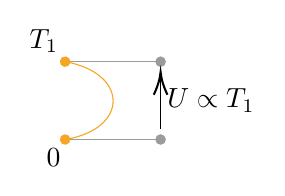
\begin{tikzpicture}[x=0.75pt,y=0.75pt,yscale=-1,xscale=1]
%uncomment if require: \path (0,110); %set diagram left start at 0, and has height of 110

%Straight Lines [id:da7792536568228223] 
\draw [color={rgb, 255:red, 155; green, 155; blue, 155 }  ,draw opacity=1 ]   (56.5,30) -- (102.5,30) ;
\draw [shift={(102.5,30)}, rotate = 0] [color={rgb, 255:red, 155; green, 155; blue, 155 }  ,draw opacity=1 ][fill={rgb, 255:red, 155; green, 155; blue, 155 }  ,fill opacity=1 ][line width=0.75]      (0, 0) circle [x radius= 2.01, y radius= 2.01]   ;
%Straight Lines [id:da7167294427341737] 
\draw [color={rgb, 255:red, 155; green, 155; blue, 155 }  ,draw opacity=1 ]   (56.5,67.5) -- (102.5,67.5) ;
\draw [shift={(102.5,67.5)}, rotate = 0] [color={rgb, 255:red, 155; green, 155; blue, 155 }  ,draw opacity=1 ][fill={rgb, 255:red, 155; green, 155; blue, 155 }  ,fill opacity=1 ][line width=0.75]      (0, 0) circle [x radius= 2.01, y radius= 2.01]   ;
%Straight Lines [id:da9591304964904978] 
\draw    (102.5,62.5) -- (102.5,37) ;
\draw [shift={(102.5,35)}, rotate = 450] [color={rgb, 255:red, 0; green, 0; blue, 0 }  ][line width=0.75]    (10.93,-3.29) .. controls (6.95,-1.4) and (3.31,-0.3) .. (0,0) .. controls (3.31,0.3) and (6.95,1.4) .. (10.93,3.29)   ;
%Curve Lines [id:da009398754899943462] 
\draw [color={rgb, 255:red, 245; green, 166; blue, 35 }  ,draw opacity=1 ]   (56.5,30) .. controls (87.33,35.5) and (87.33,62.5) .. (56.5,67.5) ;
\draw [shift={(56.5,67.5)}, rotate = 170.79] [color={rgb, 255:red, 245; green, 166; blue, 35 }  ,draw opacity=1 ][fill={rgb, 255:red, 245; green, 166; blue, 35 }  ,fill opacity=1 ][line width=0.75]      (0, 0) circle [x radius= 2.01, y radius= 2.01]   ;
\draw [shift={(56.5,30)}, rotate = 10.11] [color={rgb, 255:red, 245; green, 166; blue, 35 }  ,draw opacity=1 ][fill={rgb, 255:red, 245; green, 166; blue, 35 }  ,fill opacity=1 ][line width=0.75]      (0, 0) circle [x radius= 2.01, y radius= 2.01]   ;
% Text Node
\draw (54.5,27) node [anchor=south east] [inner sep=0.75pt]   [align=left] {$T_{1}$};
% Text Node
\draw (55.5,70.5) node [anchor=north east] [inner sep=0.75pt]   [align=left] {\SI{0}{\celsius}};
% Text Node
\draw (104.5,48.75) node [anchor=west] [inner sep=0.75pt]   [align=left] {$U \propto T_{1}$};
\end{tikzpicture}
\end{figure}
On peut déterminer $U$ à partir d'une température lorsqu'on connait précisément la mesure de $U$ à la valeur $T_2 = \SI{0}{\celsius}$. 
\end{exemple}

\subsubsection{Effet pyroélectrique}

Certains cristaux sont dits \emph{pyroélectriques} (le sulfate de triglycine par exemple) et présentent donc la propriété de présenter une polarisation électrique spontanée dépendant de la température du cristal. Ils comportent à leur surface des charges électriques $Q$ sur leurs surfaces et $-Q$ sur les surfaces opposées, proportionnelles à cette polarisation.



\begin{exemple}{Application de l'effet pyroélectrique}{}
~\\
\begin{figure}[H]

%lien d'édition des figures Tikz sur le site mathcha.io (rajouter le lien d'une modification effectuée sur la figure tikz avec le nom du modificateur car il n'y a qu'un lien par compte)

%lien mathcha Nom Prénom : https://www.mathcha.io/editor/5QmlWTYniVvh1nmzz0UV5K06oSl7KVnLfejoDdo


\tikzset{every picture/.style={line width=0.75pt}} %set default line width to 0.75pt        

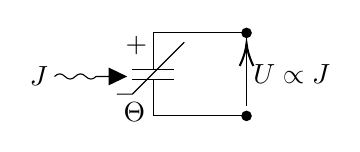
\begin{tikzpicture}[x=0.75pt,y=0.75pt,yscale=-1,xscale=1]
%uncomment if require: \path (0,110); %set diagram left start at 0, and has height of 110

%Straight Lines [id:da049441563073406525] 
\draw [color={rgb, 255:red, 0; green, 0; blue, 0 }  ,draw opacity=1 ]   (155,25) -- (200,25) ;
\draw [shift={(200,25)}, rotate = 0] [color={rgb, 255:red, 0; green, 0; blue, 0 }  ,draw opacity=1 ][fill={rgb, 255:red, 0; green, 0; blue, 0 }  ,fill opacity=1 ][line width=0.75]      (0, 0) circle [x radius= 2.01, y radius= 2.01]   ;
%Straight Lines [id:da0020140812998559188] 
\draw    (200,60) -- (200,32) ;
\draw [shift={(200,30)}, rotate = 450] [color={rgb, 255:red, 0; green, 0; blue, 0 }  ][line width=0.75]    (10.93,-3.29) .. controls (6.95,-1.4) and (3.31,-0.3) .. (0,0) .. controls (3.31,0.3) and (6.95,1.4) .. (10.93,3.29)   ;
%Straight Lines [id:da062183017724524614] 
\draw [color={rgb, 255:red, 0; green, 0; blue, 0 }  ,draw opacity=1 ]   (155,65) -- (200,65) ;
\draw [shift={(200,65)}, rotate = 0] [color={rgb, 255:red, 0; green, 0; blue, 0 }  ,draw opacity=1 ][fill={rgb, 255:red, 0; green, 0; blue, 0 }  ,fill opacity=1 ][line width=0.75]      (0, 0) circle [x radius= 2.01, y radius= 2.01]   ;
%Straight Lines [id:da18942991931898767] 
\draw    (145,42.5) -- (165,42.5) ;
%Straight Lines [id:da8438852563189819] 
\draw    (145,47.5) -- (165,47.5) ;
%Straight Lines [id:da5465187689829237] 
\draw    (155,25) -- (155,42.5) ;
%Straight Lines [id:da09145933722112254] 
\draw    (155,47.5) -- (155,65) ;

%Straight Lines [id:da8267186633709475] 
\draw    (137.5,54.5) -- (145,54.5) -- (170,29.5) ;
%Straight Lines [id:da7682659205660979] 
\draw    (107.5,46) .. controls (109.17,44.33) and (110.83,44.33) .. (112.5,46) .. controls (114.17,47.67) and (115.83,47.67) .. (117.5,46) .. controls (119.17,44.33) and (120.83,44.33) .. (122.5,46) .. controls (124.17,47.67) and (125.83,47.67) .. (127.5,46) -- (131.5,46) -- (139.5,46) ;
\draw [shift={(142.5,46)}, rotate = 180] [fill={rgb, 255:red, 0; green, 0; blue, 0 }  ][line width=0.08]  [draw opacity=0] (8.93,-4.29) -- (0,0) -- (8.93,4.29) -- cycle    ;

% Text Node
\draw (202,45) node [anchor=west] [inner sep=0.75pt]   [align=left] {$U \propto J$};
% Text Node
\draw (139.5,57.5) node [anchor=north west][inner sep=0.75pt]   [align=left] {$\Theta$};
% Text Node
\draw (140.5,25.5) node [anchor=north west][inner sep=0.75pt]   [align=left] {+};
% Text Node
\draw (105.5,46) node [anchor=east] [inner sep=0.75pt]   [align=left] {$J$};


\end{tikzpicture}

\end{figure}
On peut déterminer $U$ à partir d'un flux lumineux $J$ absorbé par un cristal pyroélectrique. Cela va élever sa température, ce qui entraîne une modification de sa polarisation qui est mesurable par la variation de tension $U$ aux bornes d'un condensateur associé.
\end{exemple}




\subsubsection{Effet piézoélectrique}

L'application d'une force ou d'une contrainte mécanique à certains matériaux dits piézoélectriques (le quartz par exemple) va entrainer une déformation provoquant l'apparition de charges électriques $Q$ sur leurs surfaces et $-Q$ sur leurs surfaces opposées.

\begin{exemple}{Application de l'effet piézoélectrique}{}
~\\
\begin{figure}[H]
\tikzset{every picture/.style={line width=0.75pt}} %set default line width to 0.75pt        

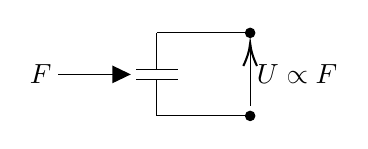
\begin{tikzpicture}[x=0.75pt,y=0.75pt,yscale=-1,xscale=1]
%uncomment if require: \path (0,110); %set diagram left start at 0, and has height of 110

%Straight Lines [id:da24742415739185752] 
\draw    (145,42.5) -- (165,42.5) ;
%Straight Lines [id:da5009949462555662] 
\draw    (145,47.5) -- (165,47.5) ;
%Straight Lines [id:da5246100942031141] 
\draw    (155,25) -- (155,42.5) ;
%Straight Lines [id:da18474784146966294] 
\draw    (155,47.5) -- (155,65) ;

%Straight Lines [id:da7890806725616728] 
\draw    (107.5,45) -- (139.5,45) ;
\draw [shift={(142.5,45)}, rotate = 180] [fill={rgb, 255:red, 0; green, 0; blue, 0 }  ][line width=0.08]  [draw opacity=0] (8.93,-4.29) -- (0,0) -- (8.93,4.29) -- cycle    ;
%Straight Lines [id:da3886370986269607] 
\draw [color={rgb, 255:red, 0; green, 0; blue, 0 }  ,draw opacity=1 ]   (155,25) -- (200,25) ;
\draw [shift={(200,25)}, rotate = 0] [color={rgb, 255:red, 0; green, 0; blue, 0 }  ,draw opacity=1 ][fill={rgb, 255:red, 0; green, 0; blue, 0 }  ,fill opacity=1 ][line width=0.75]      (0, 0) circle [x radius= 2.01, y radius= 2.01]   ;
%Straight Lines [id:da2942019649328115] 
\draw    (200,60) -- (200,32) ;
\draw [shift={(200,30)}, rotate = 450] [color={rgb, 255:red, 0; green, 0; blue, 0 }  ][line width=0.75]    (10.93,-3.29) .. controls (6.95,-1.4) and (3.31,-0.3) .. (0,0) .. controls (3.31,0.3) and (6.95,1.4) .. (10.93,3.29)   ;
%Straight Lines [id:da6965286794865602] 
\draw [color={rgb, 255:red, 0; green, 0; blue, 0 }  ,draw opacity=1 ]   (155,65) -- (200,65) ;
\draw [shift={(200,65)}, rotate = 0] [color={rgb, 255:red, 0; green, 0; blue, 0 }  ,draw opacity=1 ][fill={rgb, 255:red, 0; green, 0; blue, 0 }  ,fill opacity=1 ][line width=0.75]      (0, 0) circle [x radius= 2.01, y radius= 2.01]   ;
% Text Node
\draw (105.5,45) node [anchor=east] [inner sep=0.75pt]   [align=left] {$F$};
% Text Node
\draw (202,45) node [anchor=west] [inner sep=0.75pt]   [align=left] {$ U \propto F$};


\end{tikzpicture}
\end{figure}
On peut déterminer $U$ à partir d'une force $F$ (ou toutes grandeurs physiques dérivées) subie par l'élément piézoélectrique. Cela va provoquer une déformation de l'élément, ce qui entraine une modification de sa polarisation qui est mesurable par la variation de tension $U$ aux bornes d'un condensateur associé.
\end{exemple}


\subsubsection{Effet d'induction électromagnétique}

Lorsqu'un conducteur se déplace dans un \emph{champ magnétique} fixe $\overrightarrow{B}$, une \emph{tension} $U$ proportionnelle au \emph{flux d'induction magnétique} $\Phi$ par unité de temps $T$, et donc proportionnelle à sa vitesse de déplacement dans le champ d'induction magnétique $\overrightarrow{B}$.\\
Aussi, lorsqu'un circuit fermé est soumis à un flux d'induction magnétique $\Phi$ variable de par de son déplacement ou de celui de la source de l'induction (aimant par exemple), la tension $U$ dont il est le siège est égale au contraire de vitesse de variation du flux d'induction magnétique $\Phi$.



\begin{exemple}{Application de l'effet d'induction électromagnétique}{}
~\\
\begin{figure}[H]
\tikzset{every picture/.style={line width=0.75pt}} %set default line width to 0.75pt        

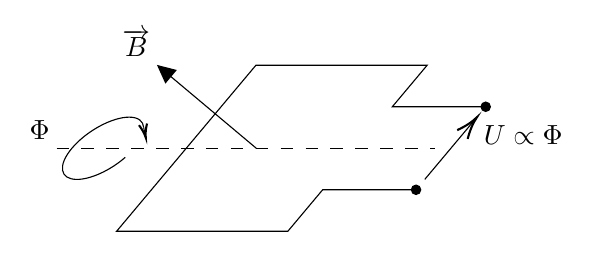
\begin{tikzpicture}[x=0.75pt,y=0.75pt,yscale=-1,xscale=1]
%uncomment if require: \path (0,156); %set diagram left start at 0, and has height of 156

%Straight Lines [id:da4159496238679624] 
\draw [color={rgb, 255:red, 0; green, 0; blue, 0 }  ,draw opacity=1 ]   (301.22,100) -- (256.22,100) -- (239.44,120) -- (156.94,120) -- (224.06,40) -- (306.56,40) -- (289.78,60) -- (334.78,60) ;
\draw [shift={(334.78,60)}, rotate = 0] [color={rgb, 255:red, 0; green, 0; blue, 0 }  ,draw opacity=1 ][fill={rgb, 255:red, 0; green, 0; blue, 0 }  ,fill opacity=1 ][line width=0.75]      (0, 0) circle [x radius= 2.01, y radius= 2.01]   ;
\draw [shift={(301.22,100)}, rotate = 180] [color={rgb, 255:red, 0; green, 0; blue, 0 }  ,draw opacity=1 ][fill={rgb, 255:red, 0; green, 0; blue, 0 }  ,fill opacity=1 ][line width=0.75]      (0, 0) circle [x radius= 2.01, y radius= 2.01]   ;
%Straight Lines [id:da9991618529346602] 
\draw    (305.41,95) -- (329.3,66.53) ;
\draw [shift={(330.59,65)}, rotate = 490] [color={rgb, 255:red, 0; green, 0; blue, 0 }  ][line width=0.75]    (10.93,-3.29) .. controls (6.95,-1.4) and (3.31,-0.3) .. (0,0) .. controls (3.31,0.3) and (6.95,1.4) .. (10.93,3.29)   ;
%Straight Lines [id:da8667170878421484] 
\draw  [dash pattern={on 4.5pt off 4.5pt}]  (128,80) -- (310.5,80) ;
%Shape: Arc [id:dp010359945518530145] 
\draw  [draw opacity=0] (161.1,84.37) .. controls (154.07,90.52) and (144.59,95) .. (137.83,95) .. controls (129.54,95) and (128.46,88.28) .. (135.41,80) .. controls (142.36,71.72) and (154.72,65) .. (163,65) .. controls (167.43,65) and (169.8,66.92) .. (169.98,69.97) -- (150.41,80) -- cycle ; \draw   (161.1,84.37) .. controls (154.07,90.52) and (144.59,95) .. (137.83,95) .. controls (129.54,95) and (128.46,88.28) .. (135.41,80) .. controls (142.36,71.72) and (154.72,65) .. (163,65) .. controls (167.43,65) and (169.8,66.92) .. (169.98,69.97) ;
%Straight Lines [id:da7991976387859124] 
\draw    (169.98,69.97) -- (170.6,72.94) ;
\draw [shift={(171.01,74.9)}, rotate = 258.2] [color={rgb, 255:red, 0; green, 0; blue, 0 }  ][line width=0.75]    (6.56,-1.97) .. controls (4.17,-0.84) and (1.99,-0.18) .. (0,0) .. controls (1.99,0.18) and (4.17,0.84) .. (6.56,1.97)   ;
%Straight Lines [id:da26501348792947876] 
\draw    (178.67,41.75) -- (224.25,80) ;
\draw [shift={(176.37,39.83)}, rotate = 40] [fill={rgb, 255:red, 0; green, 0; blue, 0 }  ][line width=0.08]  [draw opacity=0] (8.93,-4.29) -- (0,0) -- (8.93,4.29) -- cycle    ;

% Text Node
\draw (332.59,68) node [anchor=north west][inner sep=0.75pt]   [align=left] {$U \propto \Phi$};
% Text Node
\draw (174.37,36.83) node [anchor=south east] [inner sep=0.75pt]   [align=left] {$\overrightarrow{B}$};
% Text Node
\draw (126,77) node [anchor=south east] [inner sep=0.75pt]   [align=left] {$\Phi$};
\end{tikzpicture}
\end{figure}
La mesure de tension $U$ aux bornes du conducteur permet de déduire la vitesse de déplacement qui l'a induite.
\end{exemple}


\subsubsection{Effets photoélectriques}

Il existe plusieurs effets photoélectriques se distinguant par leurs manifestations mais ils ont tous comme point commun l'excitation de charges électriques dans la matière sous l'influence d'un rayonnement lumineux, dont la longueur d'onde est inférieure à une valeur seuil qui caractérise le matériau.

\begin{exemple}{Application de l'effet photoélectrique}{}
~\\
\begin{figure}[H]
\tikzset{every picture/.style={line width=0.75pt}} %set default line width to 0.75pt        

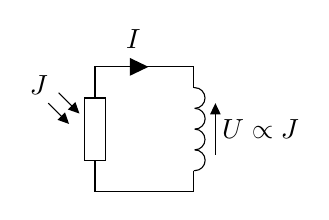
\begin{tikzpicture}[x=0.75pt,y=0.75pt,yscale=-1,xscale=1]
%uncomment if require: \path (0,153); %set diagram left start at 0, and has height of 153

%Straight Lines [id:da9553343306925111] 
\draw    (208,110.5) -- (208,115.5) ;
%Shape: Rectangle [id:dp7449879288789707] 
\draw   (213,80.5) -- (213,110.5) -- (203,110.5) -- (203,80.5) -- cycle ;
%Straight Lines [id:da5836322025533076] 
\draw    (208,75.5) -- (208,80.5) ;

%Straight Lines [id:da18940769793110568] 
\draw    (198.38,85.88) -- (190.5,78) ;
\draw [shift={(200.5,88)}, rotate = 225] [fill={rgb, 255:red, 0; green, 0; blue, 0 }  ][line width=0.08]  [draw opacity=0] (5.36,-2.57) -- (0,0) -- (5.36,2.57) -- cycle    ;
%Straight Lines [id:da5703289799533408] 
\draw    (193.38,90.88) -- (185.5,83) ;
\draw [shift={(195.5,93)}, rotate = 225] [fill={rgb, 255:red, 0; green, 0; blue, 0 }  ][line width=0.08]  [draw opacity=0] (5.36,-2.57) -- (0,0) -- (5.36,2.57) -- cycle    ;


%Straight Lines [id:da18160568852549952] 
\draw [color={rgb, 255:red, 0; green, 0; blue, 0 }  ,draw opacity=1 ]   (208,75.5) -- (208,65.5) -- (255.5,65.5) -- (255.5,75.5) ;
%Shape: Boxed Line [id:dp8550958962997346] 
\draw [color={rgb, 255:red, 0; green, 0; blue, 0 }  ,draw opacity=1 ]   (255.5,115.5) -- (255.5,125.5) -- (208,125.5) -- (208,115.5) ;
%Shape: Arc [id:dp9236278998461147] 
\draw  [draw opacity=0] (255.71,75.51) .. controls (255.81,75.5) and (255.9,75.5) .. (256,75.5) .. controls (258.76,75.5) and (261,77.74) .. (261,80.5) .. controls (261,83.25) and (258.78,85.48) .. (256.04,85.5) -- (256,80.5) -- cycle ; \draw   (255.71,75.51) .. controls (255.81,75.5) and (255.9,75.5) .. (256,75.5) .. controls (258.76,75.5) and (261,77.74) .. (261,80.5) .. controls (261,83.25) and (258.78,85.48) .. (256.04,85.5) ;
%Shape: Arc [id:dp01043642876607509] 
\draw  [draw opacity=0] (256.04,85.5) .. controls (256.05,85.5) and (256.05,85.5) .. (256.06,85.5) .. controls (258.82,85.5) and (261.06,87.74) .. (261.06,90.5) .. controls (261.06,93.25) and (258.84,95.48) .. (256.1,95.5) -- (256.06,90.5) -- cycle ; \draw   (256.04,85.5) .. controls (256.05,85.5) and (256.05,85.5) .. (256.06,85.5) .. controls (258.82,85.5) and (261.06,87.74) .. (261.06,90.5) .. controls (261.06,93.25) and (258.84,95.48) .. (256.1,95.5) ;
%Shape: Arc [id:dp6271751911575147] 
\draw  [draw opacity=0] (255.98,95.5) .. controls (255.99,95.5) and (255.99,95.5) .. (256,95.5) .. controls (258.76,95.5) and (261,97.74) .. (261,100.5) .. controls (261,103.25) and (258.78,105.48) .. (256.04,105.5) -- (256,100.5) -- cycle ; \draw   (255.98,95.5) .. controls (255.99,95.5) and (255.99,95.5) .. (256,95.5) .. controls (258.76,95.5) and (261,97.74) .. (261,100.5) .. controls (261,103.25) and (258.78,105.48) .. (256.04,105.5) ;
%Shape: Arc [id:dp7604597461390405] 
\draw  [draw opacity=0] (256.04,105.5) .. controls (256.05,105.5) and (256.05,105.5) .. (256.06,105.5) .. controls (258.82,105.5) and (261.06,107.74) .. (261.06,110.5) .. controls (261.06,113.26) and (258.82,115.5) .. (256.06,115.5) .. controls (255.9,115.5) and (255.74,115.49) .. (255.59,115.48) -- (256.06,110.5) -- cycle ; \draw   (256.04,105.5) .. controls (256.05,105.5) and (256.05,105.5) .. (256.06,105.5) .. controls (258.82,105.5) and (261.06,107.74) .. (261.06,110.5) .. controls (261.06,113.26) and (258.82,115.5) .. (256.06,115.5) .. controls (255.9,115.5) and (255.74,115.49) .. (255.59,115.48) ;

%Straight Lines [id:da7979642956460348] 
\draw    (266,86) -- (266,108) ;
\draw [shift={(266,83)}, rotate = 90] [fill={rgb, 255:red, 0; green, 0; blue, 0 }  ][line width=0.08]  [draw opacity=0] (5.36,-2.57) -- (0,0) -- (5.36,2.57) -- cycle    ;
%Straight Lines [id:da6970578975487184] 
\draw    (232.75,65.5) -- (255.5,65.5) ;
\draw [shift={(233.75,65.5)}, rotate = 180] [fill={rgb, 255:red, 0; green, 0; blue, 0 }  ][line width=0.08]  [draw opacity=0] (8.93,-4.29) -- (0,0) -- (8.93,4.29) -- cycle    ;

% Text Node
\draw (186.5,80) node [anchor=south east] [inner sep=0.75pt]   [align=left] {$J$};
% Text Node
\draw (268,95.5) node [anchor=west] [inner sep=0.75pt]   [align=left] {$U \propto J$};
% Text Node
\draw (226.5,58) node [anchor=south] [inner sep=0.75pt]   [align=left] {$I$};


\end{tikzpicture}
\end{figure}
Les effets photoélectriques permettent d'obtenir une tension $U$ ou un courant $I$ en fonction du rayonnement lumineux $J$ du matériau. D'une part, ils constituent la base des méthodes de mesure des grandeurs photométriques, d'autre part, ils permettent la traduction en signal électriques des informations véhiculées par un rayonnement lumineux.
\end{exemple}



\subsubsection{Effets photoémissif}

Les électrons libérés sont émis hors d'une zone éclairée et, lors de l'application d'un champ électrique, forment un courant électrique.

\subsubsection{Effets photovoltaïque}

Des électrons et des trous pouvant recevoir des électrons sont libérés au voisinage de la jonction Positive Négative (PN) d'un semi-conducteur éclairée. Leur déplacement dans le champ électrique de la jonction PN module la tension aux bornes de cette jonction.

\subsubsection{Effet photoélectromagnétique}

L'application d'un champ magnétique perpendiculaire à un rayonnement lumineux va provoquer dans le matériaux éclairé l'apparition d'une tension électrique dans la direction \emph{normale} au champ magnétique et au rayonnement.

\subsubsection{Effet Hall}

Un matériau, de préférence semi-conducteur et sous forme de plaquette, fait apparaitre une tension $v_{H}$ lorsqu'il est parcouru par un courant $I$ et soumis à un champ magnétique $\overrightarrow{B}$ d'un angle $\theta$ avec le courant $I$.

\begin{formule}{Effet Hall}{effet_hall}
\begin{align*}
v_H &= K_H \times I \times B \times \sin\theta
\end{align*}

\begin{textvariables}
\K_H							& coefficient	& 				& 		/											& 	Facteur dépendant du matériau et de la dimension de la plaquette \\
I									& intensité		& 	ampère			& 		\ampere					& Source de courant fournissant l'énergie liée au signal de sortie  \\
\overrightarrow{B}									& champ magnétique		& Tesla		& \tesla						& Champ magnétique soumis au matériau \\
\sin\theta					& angle							& radian		& \radian				& Angle formé par l'intensité $I$ et le champ magnétique $\overrightarrow{B}$ \\
\end{textvariables}
\end{formule}


\begin{exemple}{Application de l'effet Hall}{}
~\\
\begin{figure}[H]

\tikzset{every picture/.style={line width=0.75pt}} %set default line width to 0.75pt        

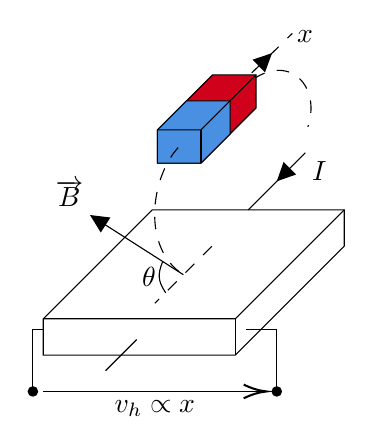
\begin{tikzpicture}[x=0.75pt,y=0.75pt,yscale=-1,xscale=1]
%uncomment if require: \path (0,255); %set diagram left start at 0, and has height of 255

%Curve Lines [id:da026480600050421743] 
\draw  [dash pattern={on 4.5pt off 4.5pt}]  (390,37.5) .. controls (411.6,12.4) and (432.3,30.3) .. (425,52.5) ;
%Shape: Cube [id:dp07360762187167524] 
\draw  [fill={rgb, 255:red, 208; green, 2; blue, 27 }  ,fill opacity=1 ] (352.5,54.06) -- (379.06,27.5) -- (400,27.5) -- (400,43.44) -- (373.44,70) -- (352.5,70) -- cycle ; \draw   (400,27.5) -- (373.44,54.06) -- (352.5,54.06) ; \draw   (373.44,54.06) -- (373.44,70) ;
%Shape: Cube [id:dp18529556990685714] 
\draw  [fill={rgb, 255:red, 74; green, 144; blue, 226 }  ,fill opacity=1 ] (352.5,54) -- (366.5,40) -- (387.5,40) -- (387.5,56) -- (373.5,70) -- (352.5,70) -- cycle ; \draw   (387.5,40) -- (373.5,54) -- (352.5,54) ; \draw   (373.5,54) -- (373.5,70) ;

%Shape: Cube [id:dp5559755925236529] 
\draw   (297.5,145) -- (350,92.5) -- (442.5,92.5) -- (442.5,110) -- (390,162.5) -- (297.5,162.5) -- cycle ; \draw   (442.5,92.5) -- (390,145) -- (297.5,145) ; \draw   (390,145) -- (390,162.5) ;
%Straight Lines [id:da7084755043157218] 
\draw    (327.5,170) -- (342.5,155) ;
%Straight Lines [id:da9878757017878151] 
\draw    (396.25,92.5) -- (423.75,65) ;
\draw [shift={(410,78.75)}, rotate = 315] [fill={rgb, 255:red, 0; green, 0; blue, 0 }  ][line width=0.08]  [draw opacity=0] (8.93,-4.29) -- (0,0) -- (8.93,4.29) -- cycle    ;
%Straight Lines [id:da6115380075011939] 
\draw    (297.5,145) -- (390,145) ;
%Straight Lines [id:da8865101665838837] 
\draw  [dash pattern={on 4.5pt off 4.5pt}]  (378.75,110) -- (351.25,137.5) ;
%Straight Lines [id:da4151864093884584] 
\draw    (322.53,96.62) -- (365,123.75) ;
\draw [shift={(320,95)}, rotate = 32.57] [fill={rgb, 255:red, 0; green, 0; blue, 0 }  ][line width=0.08]  [draw opacity=0] (8.93,-4.29) -- (0,0) -- (8.93,4.29) -- cycle    ;
%Straight Lines [id:da13161923838594092] 
\draw  [dash pattern={on 4.5pt off 4.5pt}]  (397.97,26.5) -- (417.5,7.5) ;
\draw [shift={(407.73,17)}, rotate = 495.79] [fill={rgb, 255:red, 0; green, 0; blue, 0 }  ][line width=0.08]  [draw opacity=0] (8.93,-4.29) -- (0,0) -- (8.93,4.29) -- cycle    ;
%Curve Lines [id:da8220459438720412] 
\draw  [dash pattern={on 4.5pt off 4.5pt}]  (362.5,62.5) .. controls (349.4,76.7) and (344.6,110.7) .. (365,123.75) ;
%Curve Lines [id:da48302895341966623] 
\draw    (355,117.5) .. controls (352.6,123.5) and (352.6,126.7) .. (356.5,132.5) ;
%Straight Lines [id:da0016723825185572805] 
\draw    (410,180) -- (410,150) -- (395,150) ;
\draw [shift={(410,180)}, rotate = 270] [color={rgb, 255:red, 0; green, 0; blue, 0 }  ][fill={rgb, 255:red, 0; green, 0; blue, 0 }  ][line width=0.75]      (0, 0) circle [x radius= 2.01, y radius= 2.01]   ;
%Straight Lines [id:da6665646722680143] 
\draw    (292.5,180) -- (292.5,150) -- (297.5,150) ;
\draw [shift={(292.5,180)}, rotate = 270] [color={rgb, 255:red, 0; green, 0; blue, 0 }  ][fill={rgb, 255:red, 0; green, 0; blue, 0 }  ][line width=0.75]      (0, 0) circle [x radius= 2.01, y radius= 2.01]   ;
%Straight Lines [id:da45157029340764043] 
\draw    (297.5,180) -- (403,180) ;
\draw [shift={(405,180)}, rotate = 180] [color={rgb, 255:red, 0; green, 0; blue, 0 }  ][line width=0.75]    (10.93,-3.29) .. controls (6.95,-1.4) and (3.31,-0.3) .. (0,0) .. controls (3.31,0.3) and (6.95,1.4) .. (10.93,3.29)   ;

% Text Node
\draw (425.75,68) node [anchor=north west][inner sep=0.75pt]   [align=left] {$I$};
% Text Node
\draw (318,92) node [anchor=south east] [inner sep=0.75pt]   [align=left] {$\overrightarrow{B}$};
% Text Node
\draw (353,125) node [anchor=east] [inner sep=0.75pt]   [align=left] {$\theta$};
% Text Node
\draw (418.5,5) node [anchor=north west][inner sep=0.75pt]   [align=left] {$x$};
% Text Node
\draw (351.25,183) node [anchor=north] [inner sep=0.75pt]   [align=left] {$v_{h} \propto x$};

\end{tikzpicture}
\end{figure}
Pour connaître la position de l'objet, on lui accouple un aimant qui va lui déterminer les valeurs de $\overrightarrow{B}$ et $\theta$ au niveau de la plaquette. La tension $v_{h}$ aux bornes de la plaquette est donc fonction de cet aimant et permet une conversion électrique d'une position $x$.
\end{exemple}



Il convient de classer les capteurs basés sur l'effet Hall parmi les capteurs actifs puisque l'information sortie est liée à une tension $v_H$, quand bien même il ne s'agit pas de \emph{convertisseurs d'énergie} car c'est une source de courant $I$  et non le mesurande qui va délivrer l'énergie liée au signal de sortie.

\subsection{Capteurs passifs}

Les capteurs passifs sont donc des \emph{récepteurs} qui vont voir leurs grandeurs physiques être modulées par le mesurande sans pour autant convertir une énergie. On distingue dans les récepteurs plusieurs grandeurs physiques liées à :
\begin{itemize}
\item leur géométrie et leurs dimensions\,;
\item leurs propriétés électriques :
\begin{itemize}
\item résistivité $\rho$\,;
\item perméabilité magnétique $\mu$\,;
\item constante diélectrique $\varepsilon$.
\end{itemize}
\end{itemize}

Un mesurande module donc sur la variation du signal de sortie électrique du capteur passif :
\begin{itemize}
\item soit par les caractéristiques géométriques ou des dimensions\,;
\item soit par les propriétés électriques des matériaux\,;
\item soit plus rarement par les deux à la fois.
\end{itemize}

\subsubsection{Paramètres géométrique et dimensionnel du capteur passif}

Pour que les paramètres géométriques ou dimensionnels du capteur passif puissent varier, il faut que le capteur comporte des éléments mobiles ou déformables.\\

\paragraph{Position}

Le principe d'une majorité de capteurs de déplacement et de position se base sur un élément mobile du capteur qui présente des positions spécifiques pour des valeurs de sorties précises. La mesure de cette valeur de sortie permet de connaître la position de l'élément mobile (potentiomètre, condensateur à armature mobile, inductance à noyau mobile\ldots).

\paragraph{Déformation}

La déformation est la résultante de forces -- ou de grandeurs dérivées --  qui est appliquée directement ou indirectement sur un capteur (armature d'un condensateur soumis à une pression différentielle, jauge d'extensométrie liée de manière rigide à une structure contrainte\ldots).\\
Cela entraine une modification du signal du sortie $s$, qui sera corrélée à la valeur de la force appliquée sur le capteur.

\paragraph{Propriétés électriques des matériaux}

Les propriétés électriques des matériaux varient selon leur nature et sont également sensibles à diverses grandeurs physiques (température, pression, humidité, éclairement\ldots).\\
Dans le cas ou seule l'une de ces grandeurs est susceptible de modifier les propriétés électriques d'un matériau mais que les autres n'influencent pas ces mêmes propriétés, il s'établit alors une corrélation entre ces cette grandeur physique et le signal de sortie $s$.

\begin{table}[H]
\caption{Capteurs passifs principaux selon les effets physiques}

\begin{tabularx}{\linewidth}{XX>{\compress}X}
\toprule
\thead{Mesurande}						&	\thead{Caractéristique électrique sensible}					&	\thead{Matériau utilisé} \\
\midrule
Température									& Résistivité						& 
\begin{tabitemize}
\item métaux (platine, cuivre, nickel)\,;
\item semi-conducteurs.
\end{tabitemize}
 \\
 Très basse température				& Constante diélectrique				& Verre \\
\addlinespace
Flux de rayonnement optique			& Résistivité									& Semi-conducteurs \\
\addlinespace
Déformation									& 	Résistivité		 											& \begin{tabitemize}
\item alliages de nickel\,;
\item silicium dopé.
\end{tabitemize}
 \\
													& 	Perméabilité magnétique						& 	Alliages ferromagnétiques		 \\
\addlinespace
Position (aimant)											& 	Résistivité		& 	Matériaux magnéto-résistant (bismuth, antimoniure d'indium)		 \\
\addlinespace
Humidité									&  Résistivité													& 	Chlorure de lithium		 \\
									&  Constante diélectrique								& 	Alumine, polymères		 \\
\addlinespace
Niveau							& 	Constante diélectrique								& Liquides isolants \\
\bottomrule
\end{tabularx}
\end{table}

Dans le tableau ci-dessus, on remarque l'importe de la propriété de la \emph{résistivité} $\rhoup$.\\
Le signal de sortie $s$ des \emph{capteurs passifs} n'est mesurable qu'en intégrant le capteur dans un circuit électrique alimenté, désigné comme étant son \emph{conditionneur}. Ils en existe plusieurs sortes dont les principaux sont les suivants :
\begin{description}
\item [montage potentiométrique :] association \emph{en série} d'un capteur et d'une impédance pouvant être ou non du même type\,;
\item [pont d'impédances :] équilibre électrique du pont permettant la détermination de l'impédance de sortie du capteur ou déséquilibre du pont permettant la mesure de la variation de cette impédance\,;
\item [circuit oscillant :] circuit contenant l'impédance du capteur et faisant partie d'un circuit oscillateur dont il détermine la fréquence\,;
\item [amplificateur opérationnel :] circuit dont l'impédance du capteur constitue l'un des éléments déterminant le gain de l'amplificateur.
\end{description}

Choisir un \emph{conditionneur} est une étape primordiale dans la réalisation de mesures. L'association d'un capteur et de son conditionneur -- dont sa constitution -- déterminera le signal électrique et en découleront un bon nombre de performances de mesures :
\begin{itemize}
\item sensibilité\,;
\item linéarité\,;
\item insensibilité à certaines grandeurs d'influences.
\end{itemize}

\section{Corps d'épreuves et capteurs composites}

Pour certaines raisons (coût, facilité d'exploitation\ldots), on peut utiliser des capteur sensible à l'un des effets du \emph{mesurande} plutôt qu'au mesurande lui-même.

\begin{definition}{Corps d'épreuve}{}
Dispositif de mesure qui, une fois soumis à un mesurande désigné \emph{mesurande primaire} dont il faut connaitre la grandeur, assure la traduction en une autre grandeur physique non-électrique désignée \emph{mesurande secondaire}.
\end{definition}
\begin{definition}{Capteur composite}{}
Ensemble formé par le corps d'épreuve et un capteur passif ou actif nécessaire à la traduction du mesurande secondaire donnée par le corps d'épreuve.
\end{definition}

%--------------------------------------
%CANEVAS
%--------------------------------------

%utiliser les environnement \begin{comment} \end{comment} pour mettre en commentaire le préambule une fois la programmation appelée dans le document maître (!ne pas oublier de mettre en commentaire \end{document}!)

\begin{comment}

\documentclass[a4paper, 11pt, twoside, fleqn]{memoir}

\usepackage{AOCDTF}

\marqueurchapitre
\decoupagechapitre{1} %juste pour éviter les erreurs lors de la compilation des sous-programmations (passera en commentaire)

%lien d'édition des figures Tikz sur le site mathcha.io (rajouter le lien d'une modification effectuée sur la figure tikz avec le nom du modificateur car il n'y a qu'un lien par compte) 

%lien mathcha Nom Prénom : https://www.mathcha.io/editor/88XmJTWQUxztLv21v6S12z22Lf78mx9yIOvQ9M5

%--------------------------------------
%corps du document
%--------------------------------------

\begin{document} %corps du document
	\openleft %début de chapitre à gauche

\end{comment}

\begin{figure}[h]
\caption{Structure d'un corps d'épreuve}

\tikzset{every picture/.style={line width=0.75pt}} %set default line width to 0.75pt        

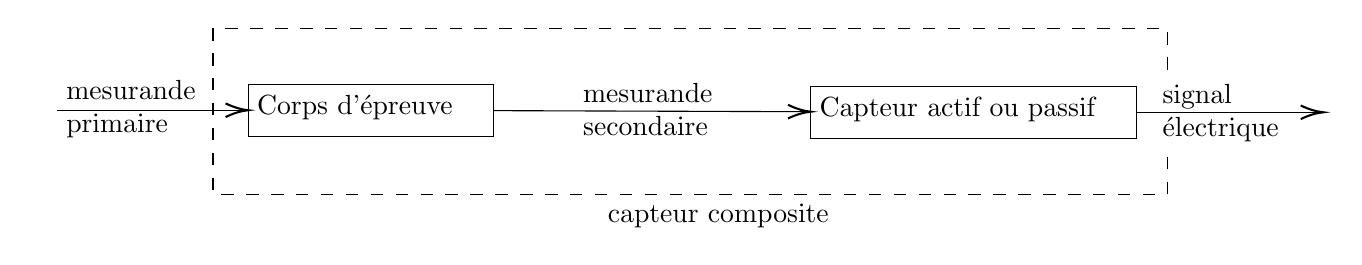
\begin{tikzpicture}[x=0.75pt,y=0.75pt,yscale=-1,xscale=1]
%uncomment if require: \path (0,300); %set diagram left start at 0, and has height of 300

%Straight Lines [id:da6331649314862131] 
\draw  [dash pattern={on 4.5pt off 4.5pt}]  (550,120) -- (550,100) -- (90,100) -- (90,180) -- (550,180) -- (550,160) ;

% Text Node
\draw    (107,127) -- (225,127) -- (225,152) -- (107,152) -- cycle  ;
\draw (110,131) node [anchor=north west][inner sep=0.75pt]   [align=left] {Corps d'épreuve};
% Text Node
\draw    (378,128) -- (535,128) -- (535,153) -- (378,153) -- cycle  ;
\draw (381,132) node [anchor=north west][inner sep=0.75pt]   [align=left] {Capteur actif ou passif};
% Text Node
\draw (1,131) node [anchor=north west][inner sep=0.75pt]   [align=left] {};
% Text Node
\draw (50.5,139) node   [align=left] {mesurande\\primaire};
% Text Node
\draw (299.5,139) node   [align=left] {mesurande\\secondaire};
% Text Node
\draw (628,132) node [anchor=north west][inner sep=0.75pt]   [align=left] {};
% Text Node
\draw (575.5,141) node   [align=left] {signal\\électrique};
% Text Node
\draw (333.5,190.5) node   [align=left] {capteur composite};
% Connection
\draw    (225,139.7) -- (376,140.22) ;
\draw [shift={(378,140.23)}, rotate = 180.2] [color={rgb, 255:red, 0; green, 0; blue, 0 }  ][line width=0.75]    (10.93,-3.29) .. controls (6.95,-1.4) and (3.31,-0.3) .. (0,0) .. controls (3.31,0.3) and (6.95,1.4) .. (10.93,3.29)   ;
% Connection
\draw    (15,139.5) -- (105,139.5) ;
\draw [shift={(107,139.5)}, rotate = 180] [color={rgb, 255:red, 0; green, 0; blue, 0 }  ][line width=0.75]    (10.93,-3.29) .. controls (6.95,-1.4) and (3.31,-0.3) .. (0,0) .. controls (3.31,0.3) and (6.95,1.4) .. (10.93,3.29)   ;
% Connection
\draw    (535,140.5) -- (623,140.5) ;
\draw [shift={(625,140.5)}, rotate = 180] [color={rgb, 255:red, 0; green, 0; blue, 0 }  ][line width=0.75]    (10.93,-3.29) .. controls (6.95,-1.4) and (3.31,-0.3) .. (0,0) .. controls (3.31,0.3) and (6.95,1.4) .. (10.93,3.29)   ;

\end{tikzpicture}
\end{figure}

%\end{document}



\begin{exemple}{Application d'un capteur composite}{}
Une force de traction $F$ est appliquée sur un objet d'une section $S$ et d'une longueur $L$, qui va subir un allongement de sa longueur $\frac{\Delta L}{L}$, entrainant de ce fait une variation de la résistance d'une jauge \Circled{1} d'un facteur $K$ placée sur l'objet $\frac{\Delta R}{R}$.
\begin{formule*}{Module de Young}{}
\begin{align*}
		E 	&= \frac{\varepsilon}{\sigma}
\end{align*}
\begin{textvariables}
E 					& Pression		&	Pascal			& \pascal 				& Module de Young (de traction) d'un matérieau \emph{élastique} et \emph{isotope} \\ 
\varepsilon	& Mètre			& 	Mètre			& \meter				& Allongement relatif (déformation) $\frac{\Delta L}{L}$ \\
 \sigma			& Pression		&	Pascal			& \pascal				& contrainte sur le matériau \\
\end{textvariables}
\end{formule*}

\begin{center}
%https://www.mathcha.io/editor/Gq5WKTE5SOVh1Y2BNvf3MWGXJHB9DB8dFlvmpqK
% Pattern Info
 
\tikzset{
pattern size/.store in=\mcSize, 
pattern size = 5pt,
pattern thickness/.store in=\mcThickness, 
pattern thickness = 0.3pt,
pattern radius/.store in=\mcRadius, 
pattern radius = 1pt}
\makeatletter
\pgfutil@ifundefined{pgf@pattern@name@_23ewa924x}{
\pgfdeclarepatternformonly[\mcThickness,\mcSize]{_23ewa924x}
{\pgfqpoint{0pt}{0pt}}
{\pgfpoint{\mcSize+\mcThickness}{\mcSize+\mcThickness}}
{\pgfpoint{\mcSize}{\mcSize}}
{
\pgfsetcolor{\tikz@pattern@color}
\pgfsetlinewidth{\mcThickness}
\pgfpathmoveto{\pgfqpoint{0pt}{0pt}}
\pgfpathlineto{\pgfpoint{\mcSize+\mcThickness}{\mcSize+\mcThickness}}
\pgfusepath{stroke}
}}
\makeatother
\tikzset{every picture/.style={line width=0.5pt}} %set default line width to 0.75pt        

\begin{tikzpicture}[x=0.75pt,y=0.75pt,yscale=-0.6,xscale=0.6]
%uncomment if require: \path (0,300); %set diagram left start at 0, and has height of 300

%Shape: Can [id:dp12472449649523132] 
\draw   (134.92,100) -- (345.08,100) .. controls (350.56,100) and (355,113.43) .. (355,130) .. controls (355,146.57) and (350.56,160) .. (345.08,160) -- (134.92,160) .. controls (129.44,160) and (125,146.57) .. (125,130) .. controls (125,113.43) and (129.44,100) .. (134.92,100) .. controls (140.39,100) and (144.83,113.43) .. (144.83,130) .. controls (144.83,146.57) and (140.39,160) .. (134.92,160) ;
%Straight Lines [id:da5161240947796851] 
\draw    (135,130) -- (98,130) ;
\draw [shift={(95,130)}, rotate = 360] [fill={rgb, 255:red, 0; green, 0; blue, 0 }  ][line width=0.08]  [draw opacity=0] (8.93,-4.29) -- (0,0) -- (8.93,4.29) -- cycle    ;
%Straight Lines [id:da28806277731694174] 
\draw    (382,130) -- (355,130) ;
\draw [shift={(385,130)}, rotate = 180] [fill={rgb, 255:red, 0; green, 0; blue, 0 }  ][line width=0.08]  [draw opacity=0] (8.93,-4.29) -- (0,0) -- (8.93,4.29) -- cycle    ;
%Straight Lines [id:da3487762389054402] 
\draw  [dash pattern={on 4.5pt off 4.5pt}]  (134.92,165) -- (135,185) ;
%Straight Lines [id:da07803041607897865] 
\draw  [dash pattern={on 4.5pt off 4.5pt}]  (344.92,165) -- (345,185) ;
%Straight Lines [id:da4638976844778334] 
\draw    (137,185) -- (343,185) ;
\draw [shift={(345,185)}, rotate = 180] [color={rgb, 255:red, 0; green, 0; blue, 0 }  ][line width=0.75]    (10.93,-3.29) .. controls (6.95,-1.4) and (3.31,-0.3) .. (0,0) .. controls (3.31,0.3) and (6.95,1.4) .. (10.93,3.29)   ;
\draw [shift={(135,185)}, rotate = 0] [color={rgb, 255:red, 0; green, 0; blue, 0 }  ][line width=0.75]    (10.93,-3.29) .. controls (6.95,-1.4) and (3.31,-0.3) .. (0,0) .. controls (3.31,0.3) and (6.95,1.4) .. (10.93,3.29)   ;
%Shape: Ellipse [id:dp48131477454456484] 
\draw  [pattern=_23ewa924x,pattern size=6pt,pattern thickness=0.75pt,pattern radius=0pt, pattern color={rgb, 255:red, 0; green, 0; blue, 0}] (125,130) .. controls (125,113.43) and (129.44,100) .. (134.92,100) .. controls (140.39,100) and (144.83,113.43) .. (144.83,130) .. controls (144.83,146.57) and (140.39,160) .. (134.92,160) .. controls (129.44,160) and (125,146.57) .. (125,130) -- cycle ;
%Shape: Rectangle [id:dp9836272663606409] 
\draw  [fill={rgb, 255:red, 0; green, 0; blue, 0 }  ,fill opacity=1 ] (240,152.5) -- (270,152.5) -- (270,160) -- (240,160) -- cycle ;

% Text Node
\draw (93,130) node [anchor=east] [inner sep=0.75pt]   [align=left] {$F$};
% Text Node
\draw (387,130) node [anchor=west] [inner sep=0.75pt]   [align=left] {$F$};
% Text Node
\draw (240,188) node [anchor=north] [inner sep=0.75pt]   [align=left] {$L$};
% Text Node
\draw (91,65) node [anchor=north west][inner sep=0.75pt]   [align=left] {$S$};
% Text Node
\draw (134.92,130) node   [align=left] {};
% Text Node
\draw (272,149.5) node [anchor=south west] [inner sep=0.75pt]   [align=left] {\Circled{1}};
% Connection
\draw    (105,86.39) -- (125.29,115.96) ;
\draw [shift={(126.42,117.61)}, rotate = 235.55] [color={rgb, 255:red, 0; green, 0; blue, 0 }  ][line width=0.75]    (10.93,-3.29) .. controls (6.95,-1.4) and (3.31,-0.3) .. (0,0) .. controls (3.31,0.3) and (6.95,1.4) .. (10.93,3.29)   ;

\end{tikzpicture}
\end{center}


Dans l'exemple la relation entre le mesurande primaire, la traction $F$ et le mesurande secondaire, la déformation $\frac{\Delta L}{L}$, est :
\begin{align*}
\frac{\Delta L}{L} &= \frac{1}{E} \times \frac{F}{S} 
\end{align*}
D'autre part, la relation entre la grandeur de sortie, la variation de la résistance de la jauge $\frac{\Delta R}{R}$ et le mesurande secondaire, la déformation $\frac{\Delta L}{L}$ est :
\begin{align*}
\frac{\Delta R}{R} &= K \times \frac{\Delta L}{L}
\end{align*}
La relation de la variation de la résistance de la jauge $R$ et la traction :
\begin{align*}
\frac{\Delta R}{R} &= \frac{K}{E} \times \frac{F}{S} 
\end{align*}
\end{exemple}

Les corps d'épreuves sont très utilisés pour mesurer des grandeurs physiques en mécanique.\\
La relation entre le mesurande primaire et le mesurande secondaire est très souvent linéaire, en particulier dans le cas de déformations et déplacement résultants de contraintes mécaniques, dans les conditions limites de l'élasticité du corps d'épreuve. Les performances de l'association corps d'épreuve -- capteur doivent être déterminées par un étalonnage tenant compte des éventuelles conséquences de leur liaison par rapport à leurs caractéristiques individuelles.\\
Si de l'électronique est intégrée au capteur, il s'agira d'un \emph{capteur intégré}.

\section{Grandeurs d'influence}

Un capteur se situe dans un environnement qui le soumet à un mesurande mais également à d'autres grandeurs physiques susceptibles de biaiser la valeur de la grandeur de sortie, sans distinction d'origine du biais.

\begin{definition}{Grandeur d'influence}{}
Grandeur physique \og parasite \fg{} à laquelle la réponse d'un capteur peut être sensible.
\end{definition}

On distingue par exemple :
\begin{itemize}
\item température pouvant faire varier la réponse d'un capteur optique\,;
\item champ magnétique pouvant faire varier la réponse d'un capteur thermométrique.
\end{itemize}

Les principales grandeurs d'influences sont :
\begin{description}
\item [température :] modification des caractéristiques électriques, mécaniques et dimensionnelles des composants du capteur\,;
\item [pression, accélération, vibration :] perturbations pouvant créer des déformations et des contraintes dans certains composants du capteur, altérant ainsi sa réponse\,;
\item [humidité :] dégradation de l'isolation (capteur/environnement et composant du capteur) et perturbation de certaines propriétés électriques (constante diélectrique, résistivité\ldots)\,;
\item [champs magnétiques variables et statiques :] apparition potentielle de tension induite pouvant se superposer au signal utile en régime statique et modification des propriété électrique en régime variable\,;
\item [tension d'alimentation (amplitude et fréquence) :] grandeur de sortie du capteur dépendante de ces grandeurs de par le principe même du capteur.
\end{description}

Si l'on se réfère à la relation mesurande -- grandeur de sortie (\superref{form:grandeur_sortie}) et qu'on comptabilise l'influence de $g_1$, $g_2$\ldots, cela donne :
\begin{formule}{Grandeurs d'influence}{grandeurs_influences}
\begin{align*}
   		s &= F(m, g_1, g_2\ldots) \\
\end{align*}

\begin{textvariables}
s						& grandeur électrique	& 			& 		/					& 	Grandeur (réponse) de sortie de nature électrique (charge, tension, courant ou impédance) fonction du mesurande \\
m						& grandeur physique		& 			& 		/					& Grandeur physique d'entrée d'excitation autre qu'électrique  \\
g_1					& grandeur physique		& 			& 		/					& Grandeur physique d'influence 1  \\
g_2					& grandeur physique		& 			& 		/					& Grandeur physique d'influence 2  \\
\end{textvariables}
\end{formule}

Pour déduire la valeur de $s$ en fonction de $m$ seul, il convient de :
\begin{itemize}
\item soit de réduire l'importance des grandeurs d'influence au niveau du capteur en le protégeant par un isolement adéquat (supports antivibratoires, blindages magnétiques\ldots)\,;
\item soit de stabiliser ces grandeurs d'influences à des seuils précisément déterminés et d'étalonner le capteur dans ces conditions de fonctionnement (enceinte climatique, sources d'alimentation régulées\ldots)\,;
\item soit d'utiliser un montage pouvant compenser l'influence des perturbations. 
\end{itemize}

\section{Chaine de mesure}

\begin{definition}{Chaine de mesure}{}
Ensemble des dispositifs, y compris le capteur, dont le but est de délivrer la détermination précise de la valeur d'un mesurande dans les meilleures conditions.  
\end{definition}

En entrée de chaine, le capteur est soumis à l'action du mesurande $m$ et injectera son signal de sortie $s$ dans la chaine. En fin de chaine, le signal de sortie $s$ est converti pour rendre la lecture de la valeur du mesurande $m$ possible.
C'est l'étalonnage de la chaine de mesure dans son ensemble qui déterminera au mieux la valeur de sortie $s$ par rapport au mesurande $m$ correspondant. \\
La chaine de mesure comprend le capteur (avec son conditionneur s'il est passif) associé à un appareil de lecture dans sa forme la plus simple (thermocouple et voltmètre par exemple).\\
Toutefois, les exigences requises par les conditions d'exploitation et la recherche de performance amènent à l'introduction de nouveaux blocs fonctionnels dans la chaine de mesure. Ceux-ci servent à optimiser l'acquisition et le traitement du signal de sortie $s$, en voici les principaux :
\begin{itemize}
\item circuit de linéarisation du signal pour obtenir des données proportionnelles à celles du mesurande $m$\,;
\item amplificateur d'instrumentation ou d'isolement pour la réduction des tensions parasites de mode commun ;
\item multiplexeur, amplificateur d'instrumentation programmable, échantillonneur bloqueur, convertisseur analogique - numérique pour le traitement de l'information par calculateur (\superref{fig:exemple_chaine_mesure})\,;
\item convertisseur tension -- courant ou tension -- fréquence pour la transmission du signal à distance par câble\,;
\item modulateur de fréquence dans cas de télémesure par voie hertzienne.
\end{itemize}

\begin{figure}{\label{fig:exemple_chaine_mesure}}
\caption{Exemple d'une chaine de mesure}


\tikzset{every picture/.style={line width=0.5pt}} %set default line width to 0.75pt        

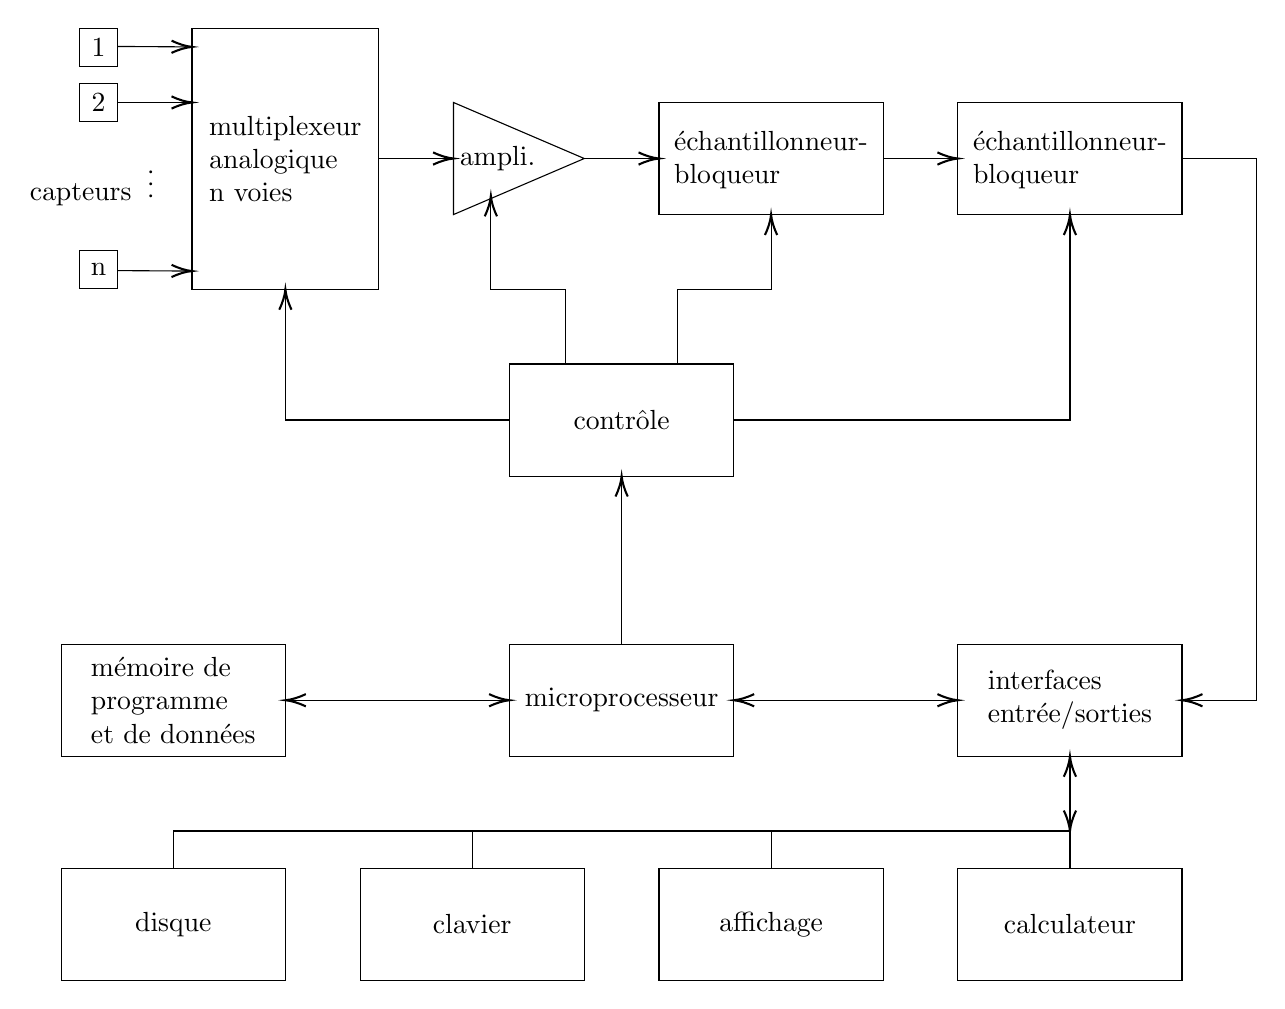
\begin{tikzpicture}[x=0.75pt,y=0.75pt,yscale=-0.9,xscale=0.9]
%uncomment if require: \path (0,542); %set diagram left start at 0, and has height of 542
%https://www.mathcha.io/editor/pJNZQf6yI3nHLEkz1QhWjMp2OT0JYgzyieBJNqK
%Flowchart: Process [id:dp6855416710808666] 
\draw   (110,10.25) -- (210,10.25) -- (210,150) -- (110,150) -- cycle ;
%Shape: Rectangle [id:dp004997227486996603] 
\draw   (50,10.25) -- (70,10.25) -- (70,30.75) -- (50,30.75) -- cycle ;
%Straight Lines [id:da4579113752456023] 
\draw    (70,20) -- (108,20.24) ;
\draw [shift={(110,20.25)}, rotate = 180.36] [color={rgb, 255:red, 0; green, 0; blue, 0 }  ][line width=0.75]    (10.93,-3.29) .. controls (6.95,-1.4) and (3.31,-0.3) .. (0,0) .. controls (3.31,0.3) and (6.95,1.4) .. (10.93,3.29)   ;
%Shape: Rectangle [id:dp6869458093862723] 
\draw   (50,39.75) -- (70,39.75) -- (70,60.25) -- (50,60.25) -- cycle ;
%Straight Lines [id:da4681455266308918] 
\draw    (70,50) -- (108,50) ;
\draw [shift={(110,50)}, rotate = 180] [color={rgb, 255:red, 0; green, 0; blue, 0 }  ][line width=0.75]    (10.93,-3.29) .. controls (6.95,-1.4) and (3.31,-0.3) .. (0,0) .. controls (3.31,0.3) and (6.95,1.4) .. (10.93,3.29)   ;
%Shape: Rectangle [id:dp45817791667488295] 
\draw   (50,129.25) -- (70,129.25) -- (70,149.75) -- (50,149.75) -- cycle ;
%Straight Lines [id:da30660098736037056] 
\draw    (70,140) -- (108,140.24) ;
\draw [shift={(110,140.25)}, rotate = 180.36] [color={rgb, 255:red, 0; green, 0; blue, 0 }  ][line width=0.75]    (10.93,-3.29) .. controls (6.95,-1.4) and (3.31,-0.3) .. (0,0) .. controls (3.31,0.3) and (6.95,1.4) .. (10.93,3.29)   ;
%Straight Lines [id:da6303825397789191] 
\draw    (210,80) -- (248,80) ;
\draw [shift={(250,80)}, rotate = 180] [color={rgb, 255:red, 0; green, 0; blue, 0 }  ][line width=0.75]    (10.93,-3.29) .. controls (6.95,-1.4) and (3.31,-0.3) .. (0,0) .. controls (3.31,0.3) and (6.95,1.4) .. (10.93,3.29)   ;
%Shape: Triangle [id:dp9560439033900896] 
\draw   (320,80) -- (250,110) -- (250,50) -- cycle ;
%Straight Lines [id:da5716448343517799] 
\draw    (320,80) -- (358,80) ;
\draw [shift={(360,80)}, rotate = 180] [color={rgb, 255:red, 0; green, 0; blue, 0 }  ][line width=0.75]    (10.93,-3.29) .. controls (6.95,-1.4) and (3.31,-0.3) .. (0,0) .. controls (3.31,0.3) and (6.95,1.4) .. (10.93,3.29)   ;
%Shape: Rectangle [id:dp5119568810350463] 
\draw   (360,50) -- (480,50) -- (480,110) -- (360,110) -- cycle ;
%Straight Lines [id:da4265953190983147] 
\draw    (480,80) -- (518,80) ;
\draw [shift={(520,80)}, rotate = 180] [color={rgb, 255:red, 0; green, 0; blue, 0 }  ][line width=0.75]    (10.93,-3.29) .. controls (6.95,-1.4) and (3.31,-0.3) .. (0,0) .. controls (3.31,0.3) and (6.95,1.4) .. (10.93,3.29)   ;
%Shape: Rectangle [id:dp7789656892769006] 
\draw   (520,50) -- (640,50) -- (640,110) -- (520,110) -- cycle ;
%Straight Lines [id:da93551183686321] 
\draw    (640,80) -- (680,80) -- (680,370) -- (642,370) ;
\draw [shift={(640,370)}, rotate = 360] [color={rgb, 255:red, 0; green, 0; blue, 0 }  ][line width=0.75]    (10.93,-3.29) .. controls (6.95,-1.4) and (3.31,-0.3) .. (0,0) .. controls (3.31,0.3) and (6.95,1.4) .. (10.93,3.29)   ;
%Shape: Rectangle [id:dp10942318417173202] 
\draw   (280,190) -- (400,190) -- (400,250) -- (280,250) -- cycle ;
%Straight Lines [id:da03354626475894362] 
\draw    (370,190) -- (370,150) -- (420,150) -- (420,112) ;
\draw [shift={(420,110)}, rotate = 450] [color={rgb, 255:red, 0; green, 0; blue, 0 }  ][line width=0.75]    (10.93,-3.29) .. controls (6.95,-1.4) and (3.31,-0.3) .. (0,0) .. controls (3.31,0.3) and (6.95,1.4) .. (10.93,3.29)   ;
%Straight Lines [id:da07083363231785789] 
\draw    (310,190) -- (310,150) -- (270,150) -- (270,102) ;
\draw [shift={(270,100)}, rotate = 450] [color={rgb, 255:red, 0; green, 0; blue, 0 }  ][line width=0.75]    (10.93,-3.29) .. controls (6.95,-1.4) and (3.31,-0.3) .. (0,0) .. controls (3.31,0.3) and (6.95,1.4) .. (10.93,3.29)   ;
%Straight Lines [id:da5566786216518755] 
\draw    (280,220) -- (160,220) -- (160,152) ;
\draw [shift={(160,150)}, rotate = 450] [color={rgb, 255:red, 0; green, 0; blue, 0 }  ][line width=0.75]    (10.93,-3.29) .. controls (6.95,-1.4) and (3.31,-0.3) .. (0,0) .. controls (3.31,0.3) and (6.95,1.4) .. (10.93,3.29)   ;
%Straight Lines [id:da44175483474459487] 
\draw    (400,220) -- (580,220) -- (580,112) ;
\draw [shift={(580,110)}, rotate = 450] [color={rgb, 255:red, 0; green, 0; blue, 0 }  ][line width=0.75]    (10.93,-3.29) .. controls (6.95,-1.4) and (3.31,-0.3) .. (0,0) .. controls (3.31,0.3) and (6.95,1.4) .. (10.93,3.29)   ;
%Straight Lines [id:da4950309462602226] 
\draw    (340,340) -- (340,252) ;
\draw [shift={(340,250)}, rotate = 450] [color={rgb, 255:red, 0; green, 0; blue, 0 }  ][line width=0.75]    (10.93,-3.29) .. controls (6.95,-1.4) and (3.31,-0.3) .. (0,0) .. controls (3.31,0.3) and (6.95,1.4) .. (10.93,3.29)   ;
%Shape: Rectangle [id:dp31894280515360696] 
\draw   (280,340) -- (400,340) -- (400,400) -- (280,400) -- cycle ;
%Shape: Rectangle [id:dp29748923859302145] 
\draw   (520,340) -- (640,340) -- (640,400) -- (520,400) -- cycle ;
%Straight Lines [id:da9319365647593406] 
\draw    (402,370) -- (518,370) ;
\draw [shift={(520,370)}, rotate = 180] [color={rgb, 255:red, 0; green, 0; blue, 0 }  ][line width=0.75]    (10.93,-3.29) .. controls (6.95,-1.4) and (3.31,-0.3) .. (0,0) .. controls (3.31,0.3) and (6.95,1.4) .. (10.93,3.29)   ;
\draw [shift={(400,370)}, rotate = 0] [color={rgb, 255:red, 0; green, 0; blue, 0 }  ][line width=0.75]    (10.93,-3.29) .. controls (6.95,-1.4) and (3.31,-0.3) .. (0,0) .. controls (3.31,0.3) and (6.95,1.4) .. (10.93,3.29)   ;
%Straight Lines [id:da5106166933182902] 
\draw    (162,370) -- (278,370) ;
\draw [shift={(280,370)}, rotate = 180] [color={rgb, 255:red, 0; green, 0; blue, 0 }  ][line width=0.75]    (10.93,-3.29) .. controls (6.95,-1.4) and (3.31,-0.3) .. (0,0) .. controls (3.31,0.3) and (6.95,1.4) .. (10.93,3.29)   ;
\draw [shift={(160,370)}, rotate = 0] [color={rgb, 255:red, 0; green, 0; blue, 0 }  ][line width=0.75]    (10.93,-3.29) .. controls (6.95,-1.4) and (3.31,-0.3) .. (0,0) .. controls (3.31,0.3) and (6.95,1.4) .. (10.93,3.29)   ;
%Shape: Rectangle [id:dp07598328049389613] 
\draw   (40,340) -- (160,340) -- (160,400) -- (40,400) -- cycle ;
%Straight Lines [id:da9982290158431298] 
\draw    (580,460) -- (580,440) -- (100,440) -- (100,460) ;
%Straight Lines [id:da9767066283683422] 
\draw    (260,440) -- (260,460) ;
%Straight Lines [id:da3569597647706805] 
\draw    (420,440) -- (420,460) ;
%Straight Lines [id:da26983482807496484] 
\draw    (580,402) -- (580,438) ;
\draw [shift={(580,440)}, rotate = 270] [color={rgb, 255:red, 0; green, 0; blue, 0 }  ][line width=0.75]    (10.93,-3.29) .. controls (6.95,-1.4) and (3.31,-0.3) .. (0,0) .. controls (3.31,0.3) and (6.95,1.4) .. (10.93,3.29)   ;
\draw [shift={(580,400)}, rotate = 90] [color={rgb, 255:red, 0; green, 0; blue, 0 }  ][line width=0.75]    (10.93,-3.29) .. controls (6.95,-1.4) and (3.31,-0.3) .. (0,0) .. controls (3.31,0.3) and (6.95,1.4) .. (10.93,3.29)   ;
%Shape: Rectangle [id:dp6771105282283583] 
\draw   (40,460) -- (160,460) -- (160,520) -- (40,520) -- cycle ;
%Shape: Rectangle [id:dp09474282891509045] 
\draw   (200,460) -- (320,460) -- (320,520) -- (200,520) -- cycle ;
%Shape: Rectangle [id:dp08838687884544572] 
\draw   (360,460) -- (480,460) -- (480,520) -- (360,520) -- cycle ;
%Shape: Rectangle [id:dp49628749586658394] 
\draw   (520,460) -- (640,460) -- (640,520) -- (520,520) -- cycle ;

% Text Node
\draw (160,80.13) node   [align=left] {multiplexeur\\analogique\\n voies};
% Text Node
\draw (60,20.5) node   [align=left] {1};
% Text Node
\draw (60,50) node   [align=left] {2};
% Text Node
\draw (60,139.5) node   [align=left] {n};
% Text Node
\draw (88,95) node  [rotate=-90] [align=left] {\ldots};
% Text Node
\draw (79,99.5) node [anchor=east] [inner sep=0.75pt]   [align=left] {capteurs};
% Text Node
\draw (252,72) node [anchor=north west][inner sep=0.75pt]   [align=left] {ampli.};
% Text Node
\draw (420,81) node   [align=left] {échantillonneur-\\bloqueur};
% Text Node
\draw (580,81) node   [align=left] {échantillonneur-\\bloqueur};
% Text Node
\draw (340,220) node   [align=left] {contrôle};
% Text Node
\draw (340,370) node   [align=left] {microprocesseur};
% Text Node
\draw (580,370) node   [align=left] {interfaces\\entrée/sorties};
% Text Node
\draw (100,370) node   [align=left] {mémoire de \\programme \\et de données};
% Text Node
\draw (100,490) node   [align=left] {disque};
% Text Node
\draw (260,490) node   [align=left] {clavier};
% Text Node
\draw (420,490) node   [align=left] {affichage};
% Text Node
\draw (580,490) node   [align=left] {calculateur};


\end{tikzpicture}
\end{figure}

Le calculateur associée à la chaine de mesure des fonctions importantes dans la chaine de mesure, elles sont regroupées dans deux catégories :
\begin{itemize}
\item gestion de l'acquisition\,;
\item traitement du signal requis par la précision et la nature de l'information cherchée.
\end{itemize}

Il gère la chaine d'acquisition en délivrant des séquences de signaux de commande. Ceux-ci vont activer de façon ordonnée les dispositifs prévus pour obtenir la valeur du mesurande $m$ :
\begin{enumerate}
\item sélection d'une voie d'entrée par envoie d'adresse au multiplexeur\,;
\item fixation du gain de l'amplificateur programmable\,;
\item échantillonnage puis blocage du signal\,;
\item déclenchement de la conversion analogique-numérique\,;
\item lecture de la donnée numérique à la réception du signal de fin de conversion délivré par le convertisseur analogique-numérique.
\end{enumerate}

En aval de la chaine d'acquisition, le calculateur gère également les périphériques d'entrée-sortie :
\begin{itemize}
\item clavier permettant l'introduction, pour prise en compte par la chaine, d'ordres et de modifications de paramètres de mesure\,;
\item mémoire de masse pour l'archivage des mesures\,;
\item affichage du résultat de la mesure en cours.
\end{itemize}

Les calculateurs permettent aussi d'effectuer des opérations mathématiques sur le signal capté et numérisé :
\begin{itemize}
\item correction du signal reçu\,;
	\begin{itemize}
	\item correction des dérives de zéro et de sensibilité causées par les grandeurs d'influences (en particulier les températures)\,;
	\item correction de la \emph{non-linéarité} des capteurs afin d'obtenir une donnée de sortie proportionnelle au mesurande\,;
	\end{itemize}
\item analyse du signal corrigé.
\end{itemize}



%\end{document}


	%--------------------------------------
%ELECTROTECHNIQUE - SCHEMA DE LIAISON A LA TERRE
%--------------------------------------

%utiliser les environnement \begin{comment} \end{comment} pour mettre en commentaire le préambule une fois la programmation appelée dans le document maître (!ne pas oublier de mettre en commentaire \end{document}!)

\begin{comment}

\documentclass[a4paper, 11pt, twoside, fleqn]{memoir}

\usepackage{AOCDTF}

\marqueurchapitre
\decoupagechapitre{1} %juste pour éviter les erreurs lors de la compilation des sous-programmations (passera en commentaire)

%--------------------------------------
%corps du document
%--------------------------------------

\begin{document} %corps du document
	\openleft %début de chapitre à gauche

\end{comment}

\chapter{Schéma Terre-Terre}
\ChapFrame

\section{Caractéristiques générales}

\begin{definition}[Schéma TT]
Schéma de liaison à la terre dans lequel :
\begin{description}
\item[Neutre :] relié à la terre\,;
\item[Masses :] reliées à la terre.
\end{description}
\end{definition}

Dans le SLT TT, le point neutre du transformateur HT/BT (point commun) est relié à la terre via la \emph{prise de terre du neutre} \Circled{1}. Cette liaison présente une certaine résistance, la \emph{résistance de la prise de terre du neutre} $R_B$ \Circled{2}. Sa mise en \oe{}uvre est à charge du fournisseur d'électricité et sa résistance globale doit être inférieure ou égale à \SI{15}{\ohm} \supercite{NF:C13-100-2015}.\\
Les masses sont quant à elles reliées à la terre via la \emph{prise de terre de l'installation électrique} \Circled{3}, qui présente aussi une certaine résistance, la \emph{résistance de la prise de terre de l'installation électrique} $R_A$ \Circled{4}. Sa mise en \oe{}uvre est à charge du propriétaire de l'installation (voir \superref{subsec:prise_terre_installation_electrique}).\\ 

Ce SLT présente les caractéristiques principales suivantes :
\begin{itemize}
\item entrainement d'une coupure de l'installation en défaut suite à une seule coupure\,;
\item simplicité à l'étude et à l'installation\,;
\item usage dans les installations alimentées directement par le réseau de distribution publique d'électricité\,;
\item protection assurée par des DDR permettant, en plus de la protection des personnes contre les contacts indirects, la prévention des risques d'incendie (lorsque leur sensibilité $I_{\Delta n}\leq\SI{300}{\milli\ampere}$).
\item permanence de surveillance en exploitation non nécessaire seulement un contrôle périodique des DDR via leur bouton test (\superref{subsubsec:principe_fonctionnement_ddr})\,;
\item possibilité de sélectivité de protection des circuits (\superref{subsubsec:selectivite_coordination_ddr})\,;
\item prise en compte d'appareils spécifiques pouvant provoquer des courants de défauts $I_d$ par le choix de DDR adaptés.
\end{itemize}

\section{Schémas de principe}

\begin{figure}[h]
\caption{Installation Terre-Terre}
\begin{subfigure}[t]{0.49\linewidth}
%--------------------------------------
%ELECTROTECHNIQUE - SCHEMA DE LIAISON A LA TERRE
%--------------------------------------

%utiliser les environnement \begin{comment} \end{comment} pour mettre en commentaire le préambule une fois la programmation appelée dans le document maître (!ne pas oublier de mettre en commentaire \end{document}!)

\begin{comment}

\documentclass[a4paper, 11pt, twoside, fleqn]{memoir}

\usepackage{AOCDTF}

\marqueurchapitre 

%lien d'édition des figures Tikz sur le site mathcha.io (rajouter le lien d'une modification effectuée sur la figure tikz avec le nom du modificateur car il n'y a qu'un lien par compte)

%lien mathcha Bruno Douchy : https://www.mathcha.io/editor/NXxYZiYwiOph2ogqzlc1q32LohL4j2ZYCPD09q3

%--------------------------------------
%corps du document
%--------------------------------------

\begin{document} %corps du document
	\openleft %début de chapitre à gauche

\end{comment}







% Pattern Info
 
\tikzset{
pattern size/.store in=\mcSize, 
pattern size = 5pt,
pattern thickness/.store in=\mcThickness, 
pattern thickness = 0.3pt,
pattern radius/.store in=\mcRadius, 
pattern radius = 1pt}
\makeatletter
\pgfutil@ifundefined{pgf@pattern@name@_04psvkee9}{
\pgfdeclarepatternformonly[\mcThickness,\mcSize]{_04psvkee9}
{\pgfqpoint{0pt}{0pt}}
{\pgfpoint{\mcSize+\mcThickness}{\mcSize+\mcThickness}}
{\pgfpoint{\mcSize}{\mcSize}}
{
\pgfsetcolor{\tikz@pattern@color}
\pgfsetlinewidth{\mcThickness}
\pgfpathmoveto{\pgfqpoint{0pt}{0pt}}
\pgfpathlineto{\pgfpoint{\mcSize+\mcThickness}{\mcSize+\mcThickness}}
\pgfusepath{stroke}
}}
\makeatother
\tikzset{every picture/.style={line width=0.5pt}} %set default line width to 0.75pt        

\begin{tikzpicture}[x=0.75pt,y=0.75pt,yscale=-0.6,xscale=0.6]
%uncomment if require: \path (0,293); %set diagram left start at 0, and has height of 293

%Shape: Rectangle [id:dp5682666133773667] 
\draw  [dash pattern={on 2.25pt off 2.25pt on 1pt off 2.25pt}] (242.5,115) -- (302.5,115) -- (302.5,145) -- (242.5,145) -- cycle ;
%Shape: Rectangle [id:dp32383377796412494] 
\draw  [dash pattern={on 2.25pt off 2.25pt on 1pt off 2.25pt}] (327.5,115) -- (387.5,115) -- (387.5,145) -- (327.5,145) -- cycle ;
%Shape: Rectangle [id:dp16529713870785345] 
\draw  [dash pattern={on 2.25pt off 2.25pt on 1pt off 2.25pt}] (412.5,115) -- (472.5,115) -- (472.5,145) -- (412.5,145) -- cycle ;
%Straight Lines [id:da25883267096548723] 
\draw [color={rgb, 255:red, 248; green, 231; blue, 28 }  ,draw opacity=1 ]   (95.5,35) -- (87.5,75) -- (87.5,182.5) ;
%Straight Lines [id:da02696774055479434] 
\draw [color={rgb, 255:red, 126; green, 211; blue, 33 }  ,draw opacity=1 ] [dash pattern={on 2.25pt off 2.25pt}]  (95.5,35) -- (87.5,75) -- (87.5,130) -- (87.5,182.5) ;
%Straight Lines [id:da80734948765028] 
\draw [color={rgb, 255:red, 74; green, 144; blue, 226 }  ,draw opacity=1 ]   (212.5,75) -- (460,75) ;
%Straight Lines [id:da004228771989997049] 
\draw [color={rgb, 255:red, 248; green, 231; blue, 28 }  ,draw opacity=1 ]   (87.5,222.5) -- (87.5,252.5) ;
%Straight Lines [id:da8023798896079356] 
\draw [color={rgb, 255:red, 248; green, 231; blue, 28 }  ,draw opacity=1 ]   (240,135) -- (225,135) -- (225,182.5) ;
%Straight Lines [id:da31232005420788] 
\draw    (212.5,35) -- (462.5,35) ;
%Straight Lines [id:da6513446287400879] 
\draw [color={rgb, 255:red, 139; green, 87; blue, 42 }  ,draw opacity=1 ]   (212.5,15) -- (462.5,15) ;
%Straight Lines [id:da8455047093895026] 
\draw [color={rgb, 255:red, 155; green, 155; blue, 155 }  ,draw opacity=1 ]   (212.5,55) -- (462.5,55) ;
%Straight Lines [id:da6574942203012859] 
\draw [color={rgb, 255:red, 74; green, 144; blue, 226 }  ,draw opacity=1 ]   (87.5,75) -- (162.5,75) ;
%Shape: Circle [id:dp2226513819215783] 
\draw  [fill={rgb, 255:red, 0; green, 0; blue, 0 }  ,fill opacity=1 ] (85,75) .. controls (85,73.62) and (86.12,72.5) .. (87.5,72.5) .. controls (88.88,72.5) and (90,73.62) .. (90,75) .. controls (90,76.38) and (88.88,77.5) .. (87.5,77.5) .. controls (86.12,77.5) and (85,76.38) .. (85,75) -- cycle ;
%Shape: Path Data [id:dp5935605530508665] 
\draw   (112.5,55) .. controls (112.5,56.38) and (111.38,57.5) .. (110,57.5) .. controls (109.29,57.5) and (108.65,57.2) .. (108.19,56.72) .. controls (102.81,61.85) and (95.52,65) .. (87.5,65) .. controls (70.93,65) and (57.5,51.57) .. (57.5,35) .. controls (57.5,18.43) and (70.93,5) .. (87.5,5) .. controls (95.52,5) and (102.81,8.15) .. (108.19,13.28) .. controls (108.65,12.8) and (109.29,12.5) .. (110,12.5) .. controls (111.38,12.5) and (112.5,13.62) .. (112.5,15) .. controls (112.5,15.82) and (112.11,16.54) .. (111.5,17) .. controls (114.8,21.39) and (116.92,26.71) .. (117.4,32.5) .. controls (117.43,32.5) and (117.47,32.5) .. (117.5,32.5) .. controls (118.88,32.5) and (120,33.62) .. (120,35) .. controls (120,36.38) and (118.88,37.5) .. (117.5,37.5) .. controls (117.47,37.5) and (117.43,37.5) .. (117.4,37.5) .. controls (116.92,43.29) and (114.8,48.61) .. (111.5,53) .. controls (112.11,53.46) and (112.5,54.18) .. (112.5,55) -- cycle ;
%Shape: Circle [id:dp9798308943037374] 
\draw   (17.5,35) .. controls (17.5,18.43) and (30.93,5) .. (47.5,5) .. controls (64.07,5) and (77.5,18.43) .. (77.5,35) .. controls (77.5,51.57) and (64.07,65) .. (47.5,65) .. controls (30.93,65) and (17.5,51.57) .. (17.5,35) -- cycle ;
%Shape: Triangle [id:dp5764497115868658] 
\draw   (40,25) -- (30,42.5) -- (50,42.5) -- cycle ;
%Shape: Star [id:dp8120117335009681] 
\draw   (106.75,35) -- (95.5,35) -- (89.88,44.81) -- (95.5,35) -- (89.88,25.19) -- (95.5,35) -- cycle ;
%Shape: Circle [id:dp5243658657822493] 
\draw   (107.5,15) .. controls (107.5,13.62) and (108.62,12.5) .. (110,12.5) .. controls (111.38,12.5) and (112.5,13.62) .. (112.5,15) .. controls (112.5,16.38) and (111.38,17.5) .. (110,17.5) .. controls (108.62,17.5) and (107.5,16.38) .. (107.5,15) -- cycle ;
%Shape: Circle [id:dp5498355617975096] 
\draw   (114.9,35) .. controls (114.9,33.62) and (116.02,32.5) .. (117.4,32.5) .. controls (118.78,32.5) and (119.9,33.62) .. (119.9,35) .. controls (119.9,36.38) and (118.78,37.5) .. (117.4,37.5) .. controls (116.02,37.5) and (114.9,36.38) .. (114.9,35) -- cycle ;
%Shape: Circle [id:dp45596527651840557] 
\draw   (107.5,55) .. controls (107.5,53.62) and (108.62,52.5) .. (110,52.5) .. controls (111.38,52.5) and (112.5,53.62) .. (112.5,55) .. controls (112.5,56.38) and (111.38,57.5) .. (110,57.5) .. controls (108.62,57.5) and (107.5,56.38) .. (107.5,55) -- cycle ;

%Straight Lines [id:da3125135145620087] 
\draw [color={rgb, 255:red, 74; green, 144; blue, 226 }  ,draw opacity=1 ]   (292.5,127.5) -- (292.5,77.5) ;
%Straight Lines [id:da21974433788696268] 
\draw [color={rgb, 255:red, 139; green, 87; blue, 42 }  ,draw opacity=1 ]   (252.5,130) -- (252.5,17.5) ;
%Straight Lines [id:da2641189769878557] 
\draw [color={rgb, 255:red, 74; green, 144; blue, 226 }  ,draw opacity=1 ]   (292.5,130.5) -- (292.5,117.5) ;
%Straight Lines [id:da3784421074756622] 
\draw    (45,232.5) -- (460,232.5) ;
%Shape: Rectangle [id:dp3931206209086823] 
\draw  [draw opacity=0][pattern=_04psvkee9,pattern size=6pt,pattern thickness=0.75pt,pattern radius=0pt, pattern color={rgb, 255:red, 0; green, 0; blue, 0}][line width=0.75]  (45,232.5) -- (460,232.5) -- (460,247.5) -- (45,247.5) -- cycle ;
%Straight Lines [id:da09075146316989513] 
\draw [color={rgb, 255:red, 126; green, 211; blue, 33 }  ,draw opacity=1 ] [dash pattern={on 2.25pt off 2.25pt}]  (240,135) -- (225,135) -- (225,182.5) ;
%Straight Lines [id:da12740897566477993] 
\draw [color={rgb, 255:red, 248; green, 231; blue, 28 }  ,draw opacity=1 ]   (225,222.5) -- (225,247.5) ;
%Straight Lines [id:da8793776219686377] 
\draw    (225,247.5) -- (225,262.5) ;
%Straight Lines [id:da6308951933981838] 
\draw    (215,262.5) -- (235,262.5) ;
%Straight Lines [id:da858762657146812] 
\draw    (217.5,267.5) -- (232.5,267.5) ;
%Straight Lines [id:da181979402279277] 
\draw    (220,272.5) -- (230,272.5) ;

%Straight Lines [id:da4986356487354773] 
\draw [color={rgb, 255:red, 126; green, 211; blue, 33 }  ,draw opacity=1 ] [dash pattern={on 2.25pt off 2.25pt}]  (225,222.5) -- (225,247.5) ;
%Straight Lines [id:da6793427381988939] 
\draw    (287.5,130) -- (292.5,130) ;
%Shape: Rectangle [id:dp761154624257314] 
\draw   (257.5,125) -- (287.5,125) -- (287.5,135) -- (257.5,135) -- cycle ;
%Straight Lines [id:da13279876059341522] 
\draw    (252.5,130) -- (257.5,130) ;

%Straight Lines [id:da18888688407013432] 
\draw    (225,217.5) -- (225,222.5) ;
%Shape: Rectangle [id:dp21719552640576667] 
\draw   (230,187.5) -- (230,217.5) -- (220,217.5) -- (220,187.5) -- cycle ;
%Straight Lines [id:da6212811003760158] 
\draw    (225,182.5) -- (225,187.5) ;

%Straight Lines [id:da16944353557480252] 
\draw [color={rgb, 255:red, 248; green, 231; blue, 28 }  ,draw opacity=1 ]   (325,135) -- (310,135) -- (310,155) -- (227.5,155.25) ;
%Straight Lines [id:da8306980458132558] 
\draw [color={rgb, 255:red, 74; green, 144; blue, 226 }  ,draw opacity=1 ]   (377.5,127.5) -- (377.5,77.5) ;
%Straight Lines [id:da3197984799192536] 
\draw [color={rgb, 255:red, 139; green, 87; blue, 42 }  ,draw opacity=1 ]   (337.5,127.5) -- (337.5,17.5) ;
%Straight Lines [id:da2129355092263585] 
\draw [color={rgb, 255:red, 139; green, 87; blue, 42 }  ,draw opacity=1 ]   (337.5,130) -- (337.5,117.5) ;
%Straight Lines [id:da5177040473827437] 
\draw [color={rgb, 255:red, 74; green, 144; blue, 226 }  ,draw opacity=1 ]   (377.5,130.5) -- (377.5,117.5) ;
%Straight Lines [id:da7711353530494354] 
\draw [color={rgb, 255:red, 126; green, 211; blue, 33 }  ,draw opacity=1 ] [dash pattern={on 2.25pt off 2.25pt}]  (325,135) -- (310,135) -- (310,155) -- (227.5,155.25) ;
%Straight Lines [id:da7033608043243165] 
\draw    (372.5,130) -- (377.5,130) ;
%Shape: Rectangle [id:dp4066961982487137] 
\draw   (342.5,125) -- (372.5,125) -- (372.5,135) -- (342.5,135) -- cycle ;
%Straight Lines [id:da9684634864445018] 
\draw    (337.5,130) -- (342.5,130) ;

%Straight Lines [id:da5416123186741061] 
\draw [color={rgb, 255:red, 248; green, 231; blue, 28 }  ,draw opacity=1 ]   (410,135) -- (395,135) -- (395,170) -- (225,170) ;
%Straight Lines [id:da9932068149507324] 
\draw [color={rgb, 255:red, 74; green, 144; blue, 226 }  ,draw opacity=1 ]   (462.5,127.5) -- (462.5,77.5) ;
%Straight Lines [id:da023330366059234442] 
\draw [color={rgb, 255:red, 139; green, 87; blue, 42 }  ,draw opacity=1 ]   (422.5,127.5) -- (422.5,17.5) ;
%Straight Lines [id:da7078047328808684] 
\draw [color={rgb, 255:red, 139; green, 87; blue, 42 }  ,draw opacity=1 ]   (422.5,130) -- (422.5,117.5) ;
%Straight Lines [id:da724301124137924] 
\draw [color={rgb, 255:red, 74; green, 144; blue, 226 }  ,draw opacity=1 ]   (462.5,130.5) -- (462.5,117.5) ;
%Straight Lines [id:da4623093821740686] 
\draw [color={rgb, 255:red, 126; green, 211; blue, 33 }  ,draw opacity=1 ] [dash pattern={on 2.25pt off 2.25pt}]  (410,135) -- (395,135) -- (395,170) -- (225,170) ;
%Straight Lines [id:da6318866740220949] 
\draw    (457.5,130) -- (462.5,130) ;
%Shape: Rectangle [id:dp8983442799253385] 
\draw   (427.5,125) -- (457.5,125) -- (457.5,135) -- (427.5,135) -- cycle ;
%Straight Lines [id:da8731453341691492] 
\draw    (422.5,130) -- (427.5,130) ;

%Shape: Circle [id:dp2874907143230092] 
\draw  [fill={rgb, 255:red, 0; green, 0; blue, 0 }  ,fill opacity=1 ] (375,75) .. controls (375,73.62) and (376.12,72.5) .. (377.5,72.5) .. controls (378.88,72.5) and (380,73.62) .. (380,75) .. controls (380,76.38) and (378.88,77.5) .. (377.5,77.5) .. controls (376.12,77.5) and (375,76.38) .. (375,75) -- cycle ;
%Shape: Circle [id:dp4786486070737942] 
\draw  [fill={rgb, 255:red, 0; green, 0; blue, 0 }  ,fill opacity=1 ] (460,75) .. controls (460,73.62) and (461.12,72.5) .. (462.5,72.5) .. controls (463.88,72.5) and (465,73.62) .. (465,75) .. controls (465,76.38) and (463.88,77.5) .. (462.5,77.5) .. controls (461.12,77.5) and (460,76.38) .. (460,75) -- cycle ;
%Shape: Circle [id:dp09552771634281954] 
\draw  [fill={rgb, 255:red, 0; green, 0; blue, 0 }  ,fill opacity=1 ] (335,15) .. controls (335,13.62) and (336.12,12.5) .. (337.5,12.5) .. controls (338.88,12.5) and (340,13.62) .. (340,15) .. controls (340,16.38) and (338.88,17.5) .. (337.5,17.5) .. controls (336.12,17.5) and (335,16.38) .. (335,15) -- cycle ;
%Shape: Circle [id:dp9468868066877425] 
\draw  [fill={rgb, 255:red, 0; green, 0; blue, 0 }  ,fill opacity=1 ] (420,15) .. controls (420,13.62) and (421.12,12.5) .. (422.5,12.5) .. controls (423.88,12.5) and (425,13.62) .. (425,15) .. controls (425,16.38) and (423.88,17.5) .. (422.5,17.5) .. controls (421.12,17.5) and (420,16.38) .. (420,15) -- cycle ;
%Shape: Circle [id:dp8031518229455832] 
\draw  [fill={rgb, 255:red, 0; green, 0; blue, 0 }  ,fill opacity=1 ] (222.5,170) .. controls (222.5,168.62) and (223.62,167.5) .. (225,167.5) .. controls (226.38,167.5) and (227.5,168.62) .. (227.5,170) .. controls (227.5,171.38) and (226.38,172.5) .. (225,172.5) .. controls (223.62,172.5) and (222.5,171.38) .. (222.5,170) -- cycle ;
%Shape: Circle [id:dp12831081640148845] 
\draw  [fill={rgb, 255:red, 0; green, 0; blue, 0 }  ,fill opacity=1 ] (290,75) .. controls (290,73.62) and (291.12,72.5) .. (292.5,72.5) .. controls (293.88,72.5) and (295,73.62) .. (295,75) .. controls (295,76.38) and (293.88,77.5) .. (292.5,77.5) .. controls (291.12,77.5) and (290,76.38) .. (290,75) -- cycle ;
%Shape: Circle [id:dp4747652428731599] 
\draw  [fill={rgb, 255:red, 0; green, 0; blue, 0 }  ,fill opacity=1 ] (250,15) .. controls (250,13.62) and (251.12,12.5) .. (252.5,12.5) .. controls (253.88,12.5) and (255,13.62) .. (255,15) .. controls (255,16.38) and (253.88,17.5) .. (252.5,17.5) .. controls (251.12,17.5) and (250,16.38) .. (250,15) -- cycle ;
%Shape: Circle [id:dp17618540641290714] 
\draw  [fill={rgb, 255:red, 0; green, 0; blue, 0 }  ,fill opacity=1 ] (222.5,155.25) .. controls (222.5,153.87) and (223.62,152.75) .. (225,152.75) .. controls (226.38,152.75) and (227.5,153.87) .. (227.5,155.25) .. controls (227.5,156.63) and (226.38,157.75) .. (225,157.75) .. controls (223.62,157.75) and (222.5,156.63) .. (222.5,155.25) -- cycle ;
%Shape: Circle [id:dp6118807302081172] 
\draw  [fill={rgb, 255:red, 255; green, 255; blue, 255 }  ,fill opacity=1 ] (240,135) .. controls (240,133.62) and (241.12,132.5) .. (242.5,132.5) .. controls (243.88,132.5) and (245,133.62) .. (245,135) .. controls (245,136.38) and (243.88,137.5) .. (242.5,137.5) .. controls (241.12,137.5) and (240,136.38) .. (240,135) -- cycle ;
%Shape: Circle [id:dp8201781923073769] 
\draw  [fill={rgb, 255:red, 255; green, 255; blue, 255 }  ,fill opacity=1 ] (250,130) .. controls (250,128.62) and (251.12,127.5) .. (252.5,127.5) .. controls (253.88,127.5) and (255,128.62) .. (255,130) .. controls (255,131.38) and (253.88,132.5) .. (252.5,132.5) .. controls (251.12,132.5) and (250,131.38) .. (250,130) -- cycle ;
%Shape: Circle [id:dp4287818286052085] 
\draw  [fill={rgb, 255:red, 255; green, 255; blue, 255 }  ,fill opacity=1 ] (290,130) .. controls (290,128.62) and (291.12,127.5) .. (292.5,127.5) .. controls (293.88,127.5) and (295,128.62) .. (295,130) .. controls (295,131.38) and (293.88,132.5) .. (292.5,132.5) .. controls (291.12,132.5) and (290,131.38) .. (290,130) -- cycle ;
%Shape: Circle [id:dp22642842975559696] 
\draw  [fill={rgb, 255:red, 255; green, 255; blue, 255 }  ,fill opacity=1 ] (325,135) .. controls (325,133.62) and (326.12,132.5) .. (327.5,132.5) .. controls (328.88,132.5) and (330,133.62) .. (330,135) .. controls (330,136.38) and (328.88,137.5) .. (327.5,137.5) .. controls (326.12,137.5) and (325,136.38) .. (325,135) -- cycle ;
%Shape: Circle [id:dp2511435925601726] 
\draw  [fill={rgb, 255:red, 255; green, 255; blue, 255 }  ,fill opacity=1 ] (335,130) .. controls (335,128.62) and (336.12,127.5) .. (337.5,127.5) .. controls (338.88,127.5) and (340,128.62) .. (340,130) .. controls (340,131.38) and (338.88,132.5) .. (337.5,132.5) .. controls (336.12,132.5) and (335,131.38) .. (335,130) -- cycle ;
%Shape: Circle [id:dp8537659771567633] 
\draw  [fill={rgb, 255:red, 255; green, 255; blue, 255 }  ,fill opacity=1 ] (375,130) .. controls (375,128.62) and (376.12,127.5) .. (377.5,127.5) .. controls (378.88,127.5) and (380,128.62) .. (380,130) .. controls (380,131.38) and (378.88,132.5) .. (377.5,132.5) .. controls (376.12,132.5) and (375,131.38) .. (375,130) -- cycle ;
%Shape: Circle [id:dp7108533568591793] 
\draw  [fill={rgb, 255:red, 255; green, 255; blue, 255 }  ,fill opacity=1 ] (410,135) .. controls (410,133.62) and (411.12,132.5) .. (412.5,132.5) .. controls (413.88,132.5) and (415,133.62) .. (415,135) .. controls (415,136.38) and (413.88,137.5) .. (412.5,137.5) .. controls (411.12,137.5) and (410,136.38) .. (410,135) -- cycle ;
%Shape: Circle [id:dp7807656659307548] 
\draw  [fill={rgb, 255:red, 255; green, 255; blue, 255 }  ,fill opacity=1 ] (420,130) .. controls (420,128.62) and (421.12,127.5) .. (422.5,127.5) .. controls (423.88,127.5) and (425,128.62) .. (425,130) .. controls (425,131.38) and (423.88,132.5) .. (422.5,132.5) .. controls (421.12,132.5) and (420,131.38) .. (420,130) -- cycle ;
%Shape: Circle [id:dp047277071011925687] 
\draw  [fill={rgb, 255:red, 255; green, 255; blue, 255 }  ,fill opacity=1 ] (460,130) .. controls (460,128.62) and (461.12,127.5) .. (462.5,127.5) .. controls (463.88,127.5) and (465,128.62) .. (465,130) .. controls (465,131.38) and (463.88,132.5) .. (462.5,132.5) .. controls (461.12,132.5) and (460,131.38) .. (460,130) -- cycle ;
%Straight Lines [id:da9839718907515904] 
\draw    (170,87.5) -- (192.5,75) -- (212.5,75) ;
%Shape: Circle [id:dp7684756542902327] 
\draw   (172.5,73) .. controls (171.4,73) and (170.5,73.9) .. (170.5,75) .. controls (170.5,76.1) and (171.4,77) .. (172.5,77) .. controls (173.6,77) and (174.5,76.1) .. (174.5,75) .. controls (174.5,73.9) and (173.6,73) .. (172.5,73) -- cycle ;
%Straight Lines [id:da6291945935079197] 
\draw    (170.5,75) -- (162.5,75) ;
%Rounded Rect [id:dp8962538925708443] 
\draw   (202.5,80) .. controls (201.12,80) and (200,78.88) .. (200,77.5) -- (200,12.5) .. controls (200,11.12) and (201.12,10) .. (202.5,10) -- (202.5,10) .. controls (203.88,10) and (205,11.12) .. (205,12.5) -- (205,77.5) .. controls (205,78.88) and (203.88,80) .. (202.5,80) -- cycle ;
%Straight Lines [id:da8998184538928884] 
\draw  [dash pattern={on 2.25pt off 2.25pt}]  (182.25,20.25) -- (182.5,85) -- (202.5,85) -- (202.5,80) ;
%Straight Lines [id:da9216978875781372] 
\draw    (170,67.5) -- (192.5,55) -- (212.5,55) ;
%Shape: Circle [id:dp7312070579582893] 
\draw   (172.5,53) .. controls (171.4,53) and (170.5,53.9) .. (170.5,55) .. controls (170.5,56.1) and (171.4,57) .. (172.5,57) .. controls (173.6,57) and (174.5,56.1) .. (174.5,55) .. controls (174.5,53.9) and (173.6,53) .. (172.5,53) -- cycle ;
%Straight Lines [id:da6058252362496683] 
\draw    (170.5,55) -- (162.5,55) ;
%Straight Lines [id:da7185616013884408] 
\draw    (170,47.5) -- (192.5,35) -- (212.5,35) ;
%Shape: Circle [id:dp7212423795898404] 
\draw   (172.5,33) .. controls (171.4,33) and (170.5,33.9) .. (170.5,35) .. controls (170.5,36.1) and (171.4,37) .. (172.5,37) .. controls (173.6,37) and (174.5,36.1) .. (174.5,35) .. controls (174.5,33.9) and (173.6,33) .. (172.5,33) -- cycle ;
%Straight Lines [id:da4153073014108539] 
\draw    (170.5,35) -- (162.5,35) ;
%Straight Lines [id:da09341299800715908] 
\draw    (170,27.5) -- (192.5,15) -- (212.5,15) ;
%Shape: Circle [id:dp05698783312682676] 
\draw   (172.5,13) .. controls (171.4,13) and (170.5,13.9) .. (170.5,15) .. controls (170.5,16.1) and (171.4,17) .. (172.5,17) .. controls (173.6,17) and (174.5,16.1) .. (174.5,15) .. controls (174.5,13.9) and (173.6,13) .. (172.5,13) -- cycle ;
%Straight Lines [id:da071527168383271] 
\draw    (170.5,15) -- (162.5,15) ;

%Straight Lines [id:da9278031736908603] 
\draw [color={rgb, 255:red, 139; green, 87; blue, 42 }  ,draw opacity=1 ]   (112.5,15) -- (162.5,15) ;
%Straight Lines [id:da8819939315013323] 
\draw [color={rgb, 255:red, 155; green, 155; blue, 155 }  ,draw opacity=1 ]   (112.5,55) -- (162.5,55) ;
%Straight Lines [id:da033362854185100876] 
\draw    (120,35) -- (162.5,35) ;
%Straight Lines [id:da11993621980114666] 
\draw    (87.5,217.5) -- (87.5,222.5) ;
%Shape: Rectangle [id:dp9514849338217106] 
\draw   (92.5,187.5) -- (92.5,217.5) -- (82.5,217.5) -- (82.5,187.5) -- cycle ;
%Straight Lines [id:da6700716558836456] 
\draw    (87.5,182.5) -- (87.5,187.5) ;

%Straight Lines [id:da7283588052348098] 
\draw [color={rgb, 255:red, 248; green, 231; blue, 28 }  ,draw opacity=1 ]   (87.5,222.5) -- (87.5,252.5) ;
%Straight Lines [id:da49077760534188997] 
\draw    (87.5,252.5) -- (87.5,267.5) ;
%Straight Lines [id:da766543912070218] 
\draw    (77.5,267.5) -- (97.5,267.5) ;
%Straight Lines [id:da18115614529294877] 
\draw    (80,272.5) -- (95,272.5) ;
%Straight Lines [id:da5181913937199873] 
\draw    (82.5,277.5) -- (92.5,277.5) ;

%Straight Lines [id:da7232122840834917] 
\draw [color={rgb, 255:red, 126; green, 211; blue, 33 }  ,draw opacity=1 ] [dash pattern={on 2.25pt off 2.25pt}]  (87.5,222.5) -- (87.5,252.5) ;
% Text Node
\draw (94.5,190.5) node [anchor=north west][inner sep=0.75pt]   [font=\footnotesize]  [align=left] {$R_B$};
% Text Node
\draw (232,190.5) node [anchor=north west][inner sep=0.75pt]  [font=\footnotesize]   [align=left] {$R_A$};
% Text Node
\draw (58,127) node [anchor=north west][inner sep=0.75pt]   [align=left] {\Circled{2}};
% Text Node
\draw (133,188) node [anchor=north west][inner sep=0.75pt]   [align=left] {\Circled{1}};
% Text Node
\draw (278,190) node [anchor=north west][inner sep=0.75pt]   [align=left] {\Circled{3}};
% Text Node
\draw (174,103) node [anchor=north west][inner sep=0.75pt]   [align=left] {\Circled{4}};
% Text Node
\draw (292,93) node [anchor=north west][inner sep=0.75pt]   [font=\footnotesize]  [align=left] {1};
% Text Node
\draw (377,93) node [anchor=north west][inner sep=0.75pt]   [font=\footnotesize]  [align=left] {2};
% Text Node
\draw (462,93) node [anchor=north west][inner sep=0.75pt] [font=\footnotesize]    [align=left] {3};
% Text Node
\draw (464,7) node [anchor=north west][inner sep=0.75pt]   [font=\footnotesize]  [align=left] {L1};
% Text Node
\draw (464,27) node [anchor=north west][inner sep=0.75pt]   [font=\footnotesize]  [align=left] {L2};
% Text Node
\draw (465,47) node [anchor=north west][inner sep=0.75pt]   [font=\footnotesize]  [align=left] {L3};
% Text Node
\draw (466.5,67) node [anchor=north west][inner sep=0.75pt]   [font=\footnotesize]  [align=left] {N};

\end{tikzpicture}


%\end{document}


\begin{comment}

\begin{circuitikz}[circuit ee IEC relay]
%\DrawGrid{(-1,-5)}{(9,3)} %grille d'aide pour le placement des objets

%sol

\fill [gray!50] (-1,-3.5) -- (5.5,-3.5) -- (5.5,-3.7) -- (-1,-3.7) -- cycle;
\draw [thick] (-1,-3.5) -- (5.5,-3.5);

%alimentation

\node (T1) [oosourcetransshape,prim=delta,sec=wye] at (0,0) {};
\node (D1) [make contact=point left, circuit breaker={point left}, tiny circuit symbols] at (1,0.45) {};
\node (D2) [make contact=point left, circuit breaker={point left}, tiny circuit symbols] at (1,0.15) {};
\node (D3) [make contact=point left, circuit breaker={point left}, tiny circuit symbols] at (1,-0.15) {};
\node (D4) [make contact=point left, circuit breaker={point left}, tiny circuit symbols] at (1,-0.45) {};

\draw [rounded corners=0.2cm] (1.4, 0.6) rectangle (1.8,-0.6);
\draw [dashed, rounded corners, thin]  (D1) to (1,-0.8) to (1.6,-0.8) to (1.6,-0.6);

\draw [brown] (-1,0.3) to (-0.5,0.3) to node {} (T1.prim1);
\draw [black] (-1,0) to (-0.5,0) to node {} (T1.prim2);
\draw [gray] (-1,-0.3) to (-0.5,-0.3) to node {} (T1.prim3);

\draw [brown] (5.5,0.45) to (D1) to (0.5,0.45) to (T1.sec1);
\draw [black] (5.5,0.15) to (D2) to (0.5,0.15) to (T1.sec2);
\draw [gray] (5.5,-0.15) to (D3) to (0.5,-0.15) to (T1.sec3);
\draw [blue] (5.5,-0.45) to (D4) to (0.5,-0.45) to (T1.sec4);

%neutre/terre

\node (RN) [resistor, label=$R_B$, rotate=90, tiny circuit symbols] at (0,-2.7) {};
\node (G1) [tlground] at (0,-3.9) {};
\draw [green!] (G1) to node {} (RN) ; 
\draw [green!] (RN) to (0,-0.5) to node {} (T1.sec4) ; 
\draw [dashed, yellow!] (G1) to node {} (RN) ;
\draw [dashed, yellow!] (RN) to (0,-0.5) to node {} (T1.sec4) ;

\node (G1) [tlground] at (0,-3.9) {};
\node (T1) [oosourcetransshape, prim=delta,sec=wye] at (0,0) {};

\node (RT) [resistor, label=$R_A$, rotate=90, tiny circuit symbols] at (2.5,-2.7) {};
\node (G2) [tlground] at (2.5,-3.9) {};
\draw [green!] (RT) to (G2); 
\draw [dashed, yellow!] (RT) to (G2);
\node (G2) [tlground] at (2.5,-3.9) {};

%appareil 1

\node (C1) [circ, scale=0.5] at (2.5,-1.8) {};
\node (C2) [circ, scale=0.5] at (2.4,0.45) {};
\node (C3) [circ, scale=0.5] at (2,-0.45) {};
\node (L) [bulb, info=1, rotate=270] at (2.4,-1.5) {};

\draw [green!] (C1) to node {} (RT); 
\draw [dashed, yellow!] (C1) to node {} (RT); 

\draw (2.1,-1.2) rectangle (2.7,-1.8);
\draw [brown] (C2) to node {} (L);
\draw [blue] (C3) to (2,-2) to (2.4,-2) to node {} (L);

%appareil 2

\node (C5) [circ, scale=0.5] at (3.7,-1.8) {};
\node (C6) [circ, scale=0.5] at (3.6,0.45) {};
\node (C7) [circ, scale=0.5] at (3.2,-0.45) {};
\node (C8) [circ, scale=0.5] at (2.5,-2.1) {};
\node (L) [bulb, info=2, rotate=270] at (3.6,-1.5) {};

\draw [green!] (C8) -| (C5); 
\draw [dashed, yellow!] (C8) -| (C5); 

\draw (3.3,-1.2) rectangle (3.9,-1.8);
\draw [brown] (C6) to node {} (L);
\draw [blue] (C7) to (3.2,-2) to (3.6,-2) to node {} (L);

%appareil 3

\node (C9) [circ, scale=0.5] at (4.9,-1.8) {};
\node (C10) [circ, scale=0.5] at (4.8,0.45) {};
\node (C11) [circ, scale=0.5] at (4.4,-0.45) {};
\node (C12) [circ, scale=0.5] at (2.5,-2.2) {};
\node (L) [bulb, info=3, rotate=270] at (4.8,-1.5) {};

\draw [green!] (C12) -| (C9); 
\draw [dashed, yellow!] (C12) -| (C9); 

\draw (4.5,-1.2) rectangle (5.1,-1.8);
\draw [brown] (C10) to node {} (L);
\draw [blue] (C11) to (4.4,-2) to (4.8,-2) to node {} (L);
%chemin courant

\callout{1,-2}{\cstep\label{pas:1}}{0.2,-3.8};
\callout{-0.5,-1}{\cstep\label{pas:2}}{-0.1,-2.4};
\callout{1.5,-3}{\cstep\label{pas:3}}{2.2,-3.8};
\callout{4,-2.6}{\cstep\label{pas:4}}{2.6,-2.6};
\startcstep %remet les compteurs des légendes en pastille à zéro
\end{circuitikz}

\end{comment}
\subcaption{sans défaut d'isolement}
\end{subfigure}
\begin{subfigure}[t]{0.49\linewidth}
%--------------------------------------
%ELECTROTECHNIQUE - SCHEMA DE LIAISON A LA TERRE
%--------------------------------------

%utiliser les environnement \begin{comment} \end{comment} pour mettre en commentaire le préambule une fois la programmation appelée dans le document maître (!ne pas oublier de mettre en commentaire \end{document}!)

\begin{comment}

\documentclass[a4paper, 11pt, twoside, fleqn]{memoir}

\usepackage{AOCDTF}

\marqueurchapitre

%lien d'édition des figures Tikz sur le site mathcha.io (rajouter le lien d'une modification effectuée sur la figure tikz avec le nom du modificateur car il n'y a qu'un lien par compte)

%lien mathcha Bruno Douchy : https://www.mathcha.io/editor/eKlmwIEXSj3Czgp1ZlU5eo1ZqI4VwNeYHpB7zQK

%--------------------------------------
%corps du document
%--------------------------------------

\begin{document} %corps du document
	\openleft %début de chapitre à gauche

\end{comment}



% Pattern Info
 
\tikzset{
pattern size/.store in=\mcSize, 
pattern size = 5pt,
pattern thickness/.store in=\mcThickness, 
pattern thickness = 0.3pt,
pattern radius/.store in=\mcRadius, 
pattern radius = 1pt}
\makeatletter
\pgfutil@ifundefined{pgf@pattern@name@_cuy0d7oml}{
\pgfdeclarepatternformonly[\mcThickness,\mcSize]{_cuy0d7oml}
{\pgfqpoint{0pt}{0pt}}
{\pgfpoint{\mcSize+\mcThickness}{\mcSize+\mcThickness}}
{\pgfpoint{\mcSize}{\mcSize}}
{
\pgfsetcolor{\tikz@pattern@color}
\pgfsetlinewidth{\mcThickness}
\pgfpathmoveto{\pgfqpoint{0pt}{0pt}}
\pgfpathlineto{\pgfpoint{\mcSize+\mcThickness}{\mcSize+\mcThickness}}
\pgfusepath{stroke}
}}
\makeatother
\tikzset{every picture/.style={line width=0.5pt}} %set default line width to 0.75pt        

\begin{tikzpicture}[x=0.75pt,y=0.75pt,yscale=-0.6,xscale=0.6]
%uncomment if require: \path (0,293); %set diagram left start at 0, and has height of 293

%Shape: Rectangle [id:dp7721912972979099] 
\draw  [dash pattern={on 2.25pt off 2.25pt on 1pt off 2.25pt}] (242.5,115) -- (302.5,115) -- (302.5,145) -- (242.5,145) -- cycle ;
%Shape: Rectangle [id:dp0573995662487482] 
\draw  [dash pattern={on 2.25pt off 2.25pt on 1pt off 2.25pt}] (327.5,115) -- (387.5,115) -- (387.5,145) -- (327.5,145) -- cycle ;
%Shape: Rectangle [id:dp4688841448778266] 
\draw  [dash pattern={on 2.25pt off 2.25pt on 1pt off 2.25pt}] (412.5,115) -- (472.5,115) -- (472.5,145) -- (412.5,145) -- cycle ;
%Straight Lines [id:da6329210676668946] 
\draw [color={rgb, 255:red, 248; green, 231; blue, 28 }  ,draw opacity=1 ]   (87.5,222.5) -- (87.5,252.5) ;
%Straight Lines [id:da0731217300744833] 
\draw [color={rgb, 255:red, 248; green, 231; blue, 28 }  ,draw opacity=1 ]   (240,135) -- (225,135) -- (225,182.5) ;
%Straight Lines [id:da20436909232284672] 
\draw    (120,35) -- (162.5,35) ;
%Straight Lines [id:da6628360702968055] 
\draw [color={rgb, 255:red, 139; green, 87; blue, 42 }  ,draw opacity=1 ]   (112.5,15) -- (162.5,15) ;
%Straight Lines [id:da6730215661783633] 
\draw [color={rgb, 255:red, 155; green, 155; blue, 155 }  ,draw opacity=1 ]   (112.5,55) -- (162.5,55) ;
%Straight Lines [id:da21679134998500837] 
\draw [color={rgb, 255:red, 74; green, 144; blue, 226 }  ,draw opacity=1 ]   (87.5,75) -- (162.5,75) ;
%Straight Lines [id:da972362966086349] 
\draw [color={rgb, 255:red, 248; green, 231; blue, 28 }  ,draw opacity=1 ]   (95.5,35) -- (87.5,75) -- (87.5,182.5) ;
%Straight Lines [id:da7325700572517352] 
\draw [color={rgb, 255:red, 126; green, 211; blue, 33 }  ,draw opacity=1 ] [dash pattern={on 2.25pt off 2.25pt}]  (95.5,35) -- (87.5,75) -- (87.5,182.5) ;
%Shape: Circle [id:dp0497230525738539] 
\draw  [fill={rgb, 255:red, 0; green, 0; blue, 0 }  ,fill opacity=1 ] (85,75) .. controls (85,73.62) and (86.12,72.5) .. (87.5,72.5) .. controls (88.88,72.5) and (90,73.62) .. (90,75) .. controls (90,76.38) and (88.88,77.5) .. (87.5,77.5) .. controls (86.12,77.5) and (85,76.38) .. (85,75) -- cycle ;
%Straight Lines [id:da24030659502468465] 
\draw    (202.5,35) -- (460,35) ;
%Straight Lines [id:da17893731437856264] 
\draw [color={rgb, 255:red, 139; green, 87; blue, 42 }  ,draw opacity=1 ]   (202.5,15) -- (460,15) ;
%Straight Lines [id:da7326617199950461] 
\draw [color={rgb, 255:red, 155; green, 155; blue, 155 }  ,draw opacity=1 ]   (202.5,55) -- (460,55) ;
%Straight Lines [id:da6422834100389347] 
\draw [color={rgb, 255:red, 74; green, 144; blue, 226 }  ,draw opacity=1 ]   (202.5,75) -- (462.5,75) ;
%Shape: Path Data [id:dp34255928615646025] 
\draw   (112.5,55) .. controls (112.5,56.38) and (111.38,57.5) .. (110,57.5) .. controls (109.29,57.5) and (108.65,57.2) .. (108.19,56.72) .. controls (102.81,61.85) and (95.52,65) .. (87.5,65) .. controls (70.93,65) and (57.5,51.57) .. (57.5,35) .. controls (57.5,18.43) and (70.93,5) .. (87.5,5) .. controls (95.52,5) and (102.81,8.15) .. (108.19,13.28) .. controls (108.65,12.8) and (109.29,12.5) .. (110,12.5) .. controls (111.38,12.5) and (112.5,13.62) .. (112.5,15) .. controls (112.5,15.82) and (112.11,16.54) .. (111.5,17) .. controls (114.8,21.39) and (116.92,26.71) .. (117.4,32.5) .. controls (117.43,32.5) and (117.47,32.5) .. (117.5,32.5) .. controls (118.88,32.5) and (120,33.62) .. (120,35) .. controls (120,36.38) and (118.88,37.5) .. (117.5,37.5) .. controls (117.47,37.5) and (117.43,37.5) .. (117.4,37.5) .. controls (116.92,43.29) and (114.8,48.61) .. (111.5,53) .. controls (112.11,53.46) and (112.5,54.18) .. (112.5,55) -- cycle ;
%Shape: Circle [id:dp028864487962136365] 
\draw   (17.5,35) .. controls (17.5,18.43) and (30.93,5) .. (47.5,5) .. controls (64.07,5) and (77.5,18.43) .. (77.5,35) .. controls (77.5,51.57) and (64.07,65) .. (47.5,65) .. controls (30.93,65) and (17.5,51.57) .. (17.5,35) -- cycle ;
%Shape: Triangle [id:dp48665526213410604] 
\draw   (40,25) -- (30,42.5) -- (50,42.5) -- cycle ;
%Shape: Star [id:dp3984898622249935] 
\draw   (106.75,35) -- (95.5,35) -- (89.88,44.81) -- (95.5,35) -- (89.88,25.19) -- (95.5,35) -- cycle ;
%Shape: Circle [id:dp18887861066852274] 
\draw   (107.5,15) .. controls (107.5,13.62) and (108.62,12.5) .. (110,12.5) .. controls (111.38,12.5) and (112.5,13.62) .. (112.5,15) .. controls (112.5,16.38) and (111.38,17.5) .. (110,17.5) .. controls (108.62,17.5) and (107.5,16.38) .. (107.5,15) -- cycle ;
%Shape: Circle [id:dp5495459619566693] 
\draw   (114.9,35) .. controls (114.9,33.62) and (116.02,32.5) .. (117.4,32.5) .. controls (118.78,32.5) and (119.9,33.62) .. (119.9,35) .. controls (119.9,36.38) and (118.78,37.5) .. (117.4,37.5) .. controls (116.02,37.5) and (114.9,36.38) .. (114.9,35) -- cycle ;
%Shape: Circle [id:dp7341713415218949] 
\draw   (107.5,55) .. controls (107.5,53.62) and (108.62,52.5) .. (110,52.5) .. controls (111.38,52.5) and (112.5,53.62) .. (112.5,55) .. controls (112.5,56.38) and (111.38,57.5) .. (110,57.5) .. controls (108.62,57.5) and (107.5,56.38) .. (107.5,55) -- cycle ;

%Straight Lines [id:da3995338827620828] 
\draw [color={rgb, 255:red, 74; green, 144; blue, 226 }  ,draw opacity=1 ]   (292.5,127.5) -- (292.5,77.5) ;
%Straight Lines [id:da11010006494259639] 
\draw [color={rgb, 255:red, 139; green, 87; blue, 42 }  ,draw opacity=1 ]   (252.5,127.5) -- (252.5,17.5) ;
%Straight Lines [id:da8401356256684356] 
\draw [color={rgb, 255:red, 139; green, 87; blue, 42 }  ,draw opacity=1 ]   (252.5,130) -- (252.5,117.5) ;
%Straight Lines [id:da5678843021306501] 
\draw [color={rgb, 255:red, 74; green, 144; blue, 226 }  ,draw opacity=1 ]   (292.5,130.5) -- (292.5,117.5) ;
%Straight Lines [id:da7747032857959617] 
\draw    (45,230) -- (460,230) ;
%Shape: Rectangle [id:dp6036556809723994] 
\draw  [draw opacity=0][pattern=_cuy0d7oml,pattern size=6pt,pattern thickness=0.75pt,pattern radius=0pt, pattern color={rgb, 255:red, 0; green, 0; blue, 0}][line width=0.75]  (45,230) -- (460,230) -- (460,245) -- (45,245) -- cycle ;
%Straight Lines [id:da8962711374370711] 
\draw [color={rgb, 255:red, 126; green, 211; blue, 33 }  ,draw opacity=1 ] [dash pattern={on 2.25pt off 2.25pt}]  (240,135) -- (225,135) -- (225,182.5) ;
%Straight Lines [id:da9054180111460266] 
\draw    (87.5,252.5) -- (87.5,267.5) ;
%Straight Lines [id:da9375498024378792] 
\draw    (77.5,267.5) -- (97.5,267.5) ;
%Straight Lines [id:da6825496272804993] 
\draw    (80,272.5) -- (95,272.5) ;
%Straight Lines [id:da9028290441872109] 
\draw    (82.5,277.5) -- (92.5,277.5) ;

%Straight Lines [id:da838749004387143] 
\draw [color={rgb, 255:red, 126; green, 211; blue, 33 }  ,draw opacity=1 ] [dash pattern={on 2.25pt off 2.25pt}]  (87.5,222.5) -- (87.5,252.5) ;
%Straight Lines [id:da6732857797704417] 
\draw [color={rgb, 255:red, 248; green, 231; blue, 28 }  ,draw opacity=1 ]   (225,222.5) -- (225,252.5) ;
%Straight Lines [id:da04423537743139716] 
\draw    (225,252.5) -- (225,267.5) ;
%Straight Lines [id:da19138853362068498] 
\draw    (215,267.5) -- (235,267.5) ;
%Straight Lines [id:da9292325270181725] 
\draw    (217.5,272.5) -- (232.5,272.5) ;
%Straight Lines [id:da6824238772465032] 
\draw    (220,277.5) -- (230,277.5) ;

%Straight Lines [id:da5881618514978333] 
\draw [color={rgb, 255:red, 126; green, 211; blue, 33 }  ,draw opacity=1 ] [dash pattern={on 2.25pt off 2.25pt}]  (225,222.5) -- (225,252.5) ;
%Straight Lines [id:da4372917094795513] 
\draw    (287.5,130) -- (292.5,130) ;
%Shape: Rectangle [id:dp6549318296691656] 
\draw   (257.5,125) -- (287.5,125) -- (287.5,135) -- (257.5,135) -- cycle ;
%Straight Lines [id:da44309459356857717] 
\draw    (252.5,130) -- (257.5,130) ;

%Straight Lines [id:da06222974092566569] 
\draw    (87.5,217.5) -- (87.5,222.5) ;
%Shape: Rectangle [id:dp9937883234958191] 
\draw   (92.5,187.5) -- (92.5,217.5) -- (82.5,217.5) -- (82.5,187.5) -- cycle ;
%Straight Lines [id:da025869666691459292] 
\draw    (87.5,182.5) -- (87.5,187.5) ;

%Straight Lines [id:da4798539028950788] 
\draw    (225,217.5) -- (225,222.5) ;
%Shape: Rectangle [id:dp2723576597961067] 
\draw   (230,187.5) -- (230,217.5) -- (220,217.5) -- (220,187.5) -- cycle ;
%Straight Lines [id:da5655528977502864] 
\draw    (225,182.5) -- (225,187.5) ;

%Straight Lines [id:da940864516854409] 
\draw [color={rgb, 255:red, 248; green, 231; blue, 28 }  ,draw opacity=1 ]   (325,135) -- (310,135) -- (310,155) -- (227.5,155.25) ;
%Straight Lines [id:da8122415118743977] 
\draw [color={rgb, 255:red, 74; green, 144; blue, 226 }  ,draw opacity=1 ]   (377.5,127.5) -- (377.5,77.5) ;
%Straight Lines [id:da6473794199105589] 
\draw [color={rgb, 255:red, 139; green, 87; blue, 42 }  ,draw opacity=1 ]   (337.5,112.5) -- (337.5,17.5) ;
%Straight Lines [id:da6567132968862988] 
\draw [color={rgb, 255:red, 139; green, 87; blue, 42 }  ,draw opacity=1 ]   (337.5,130) -- (337.5,117.5) ;
%Straight Lines [id:da8155227791109615] 
\draw [color={rgb, 255:red, 74; green, 144; blue, 226 }  ,draw opacity=1 ]   (377.5,130.5) -- (377.5,117.5) ;
%Straight Lines [id:da6972674997945025] 
\draw [color={rgb, 255:red, 126; green, 211; blue, 33 }  ,draw opacity=1 ] [dash pattern={on 2.25pt off 2.25pt}]  (325,135) -- (310,135) -- (310,155) -- (227.5,155.25) ;
%Straight Lines [id:da5069619176082795] 
\draw    (372.5,130) -- (377.5,130) ;
%Shape: Rectangle [id:dp1559843402584261] 
\draw   (342.5,125) -- (372.5,125) -- (372.5,135) -- (342.5,135) -- cycle ;
%Straight Lines [id:da9123610170199719] 
\draw    (337.5,130) -- (342.5,130) ;

%Straight Lines [id:da2598762311191992] 
\draw [color={rgb, 255:red, 248; green, 231; blue, 28 }  ,draw opacity=1 ]   (410,135) -- (395,135) -- (395,170) -- (225,170) ;
%Straight Lines [id:da4040784933658479] 
\draw [color={rgb, 255:red, 74; green, 144; blue, 226 }  ,draw opacity=1 ]   (462.5,117.5) -- (462.5,77.5) ;
%Straight Lines [id:da5604329205598866] 
\draw [color={rgb, 255:red, 139; green, 87; blue, 42 }  ,draw opacity=1 ]   (422.5,117.5) -- (422.5,17.5) ;
%Straight Lines [id:da9471353425142487] 
\draw [color={rgb, 255:red, 139; green, 87; blue, 42 }  ,draw opacity=1 ]   (422.5,130) -- (422.5,117.5) ;
%Straight Lines [id:da15807281012737096] 
\draw [color={rgb, 255:red, 74; green, 144; blue, 226 }  ,draw opacity=1 ]   (462.5,130.5) -- (462.5,117.5) ;
%Straight Lines [id:da2829658429752038] 
\draw [color={rgb, 255:red, 126; green, 211; blue, 33 }  ,draw opacity=1 ] [dash pattern={on 2.25pt off 2.25pt}]  (412.5,135) -- (395,135) -- (395,170) -- (227.5,170) ;
%Straight Lines [id:da5256750975408043] 
\draw    (457.5,130) -- (462.5,130) ;
%Shape: Rectangle [id:dp3420064291792977] 
\draw   (427.5,125) -- (457.5,125) -- (457.5,135) -- (427.5,135) -- cycle ;
%Straight Lines [id:da703886926271932] 
\draw    (422.5,130) -- (427.5,130) ;

%Shape: Circle [id:dp9542404500183199] 
\draw  [fill={rgb, 255:red, 0; green, 0; blue, 0 }  ,fill opacity=1 ] (375,75) .. controls (375,73.62) and (376.12,72.5) .. (377.5,72.5) .. controls (378.88,72.5) and (380,73.62) .. (380,75) .. controls (380,76.38) and (378.88,77.5) .. (377.5,77.5) .. controls (376.12,77.5) and (375,76.38) .. (375,75) -- cycle ;
%Shape: Circle [id:dp19958214405780028] 
\draw  [fill={rgb, 255:red, 0; green, 0; blue, 0 }  ,fill opacity=1 ] (460,75) .. controls (460,73.62) and (461.12,72.5) .. (462.5,72.5) .. controls (463.88,72.5) and (465,73.62) .. (465,75) .. controls (465,76.38) and (463.88,77.5) .. (462.5,77.5) .. controls (461.12,77.5) and (460,76.38) .. (460,75) -- cycle ;
%Shape: Circle [id:dp6770022928832852] 
\draw  [fill={rgb, 255:red, 0; green, 0; blue, 0 }  ,fill opacity=1 ] (335,15) .. controls (335,13.62) and (336.12,12.5) .. (337.5,12.5) .. controls (338.88,12.5) and (340,13.62) .. (340,15) .. controls (340,16.38) and (338.88,17.5) .. (337.5,17.5) .. controls (336.12,17.5) and (335,16.38) .. (335,15) -- cycle ;
%Shape: Circle [id:dp09638860315940234] 
\draw  [fill={rgb, 255:red, 0; green, 0; blue, 0 }  ,fill opacity=1 ] (420,15) .. controls (420,13.62) and (421.12,12.5) .. (422.5,12.5) .. controls (423.88,12.5) and (425,13.62) .. (425,15) .. controls (425,16.38) and (423.88,17.5) .. (422.5,17.5) .. controls (421.12,17.5) and (420,16.38) .. (420,15) -- cycle ;
%Shape: Circle [id:dp7650652986077244] 
\draw  [fill={rgb, 255:red, 0; green, 0; blue, 0 }  ,fill opacity=1 ] (222.5,170) .. controls (222.5,168.62) and (223.62,167.5) .. (225,167.5) .. controls (226.38,167.5) and (227.5,168.62) .. (227.5,170) .. controls (227.5,171.38) and (226.38,172.5) .. (225,172.5) .. controls (223.62,172.5) and (222.5,171.38) .. (222.5,170) -- cycle ;
%Shape: Circle [id:dp28148087795993504] 
\draw  [fill={rgb, 255:red, 0; green, 0; blue, 0 }  ,fill opacity=1 ] (290,75) .. controls (290,73.62) and (291.12,72.5) .. (292.5,72.5) .. controls (293.88,72.5) and (295,73.62) .. (295,75) .. controls (295,76.38) and (293.88,77.5) .. (292.5,77.5) .. controls (291.12,77.5) and (290,76.38) .. (290,75) -- cycle ;
%Shape: Circle [id:dp42655059796691996] 
\draw  [fill={rgb, 255:red, 0; green, 0; blue, 0 }  ,fill opacity=1 ] (250,15) .. controls (250,13.62) and (251.12,12.5) .. (252.5,12.5) .. controls (253.88,12.5) and (255,13.62) .. (255,15) .. controls (255,16.38) and (253.88,17.5) .. (252.5,17.5) .. controls (251.12,17.5) and (250,16.38) .. (250,15) -- cycle ;
%Shape: Circle [id:dp13138044107648572] 
\draw  [fill={rgb, 255:red, 0; green, 0; blue, 0 }  ,fill opacity=1 ] (222.5,155.25) .. controls (222.5,153.87) and (223.62,152.75) .. (225,152.75) .. controls (226.38,152.75) and (227.5,153.87) .. (227.5,155.25) .. controls (227.5,156.63) and (226.38,157.75) .. (225,157.75) .. controls (223.62,157.75) and (222.5,156.63) .. (222.5,155.25) -- cycle ;
%Shape: Circle [id:dp21465585762797446] 
\draw  [fill={rgb, 255:red, 255; green, 255; blue, 255 }  ,fill opacity=1 ] (240,135) .. controls (240,133.62) and (241.12,132.5) .. (242.5,132.5) .. controls (243.88,132.5) and (245,133.62) .. (245,135) .. controls (245,136.38) and (243.88,137.5) .. (242.5,137.5) .. controls (241.12,137.5) and (240,136.38) .. (240,135) -- cycle ;
%Shape: Circle [id:dp45186106918120084] 
\draw  [fill={rgb, 255:red, 255; green, 255; blue, 255 }  ,fill opacity=1 ] (250,130) .. controls (250,128.62) and (251.12,127.5) .. (252.5,127.5) .. controls (253.88,127.5) and (255,128.62) .. (255,130) .. controls (255,131.38) and (253.88,132.5) .. (252.5,132.5) .. controls (251.12,132.5) and (250,131.38) .. (250,130) -- cycle ;
%Shape: Circle [id:dp29108030649379046] 
\draw  [fill={rgb, 255:red, 255; green, 255; blue, 255 }  ,fill opacity=1 ] (290,130) .. controls (290,128.62) and (291.12,127.5) .. (292.5,127.5) .. controls (293.88,127.5) and (295,128.62) .. (295,130) .. controls (295,131.38) and (293.88,132.5) .. (292.5,132.5) .. controls (291.12,132.5) and (290,131.38) .. (290,130) -- cycle ;
%Shape: Circle [id:dp6026453317917776] 
\draw  [fill={rgb, 255:red, 255; green, 255; blue, 255 }  ,fill opacity=1 ] (325,135) .. controls (325,133.62) and (326.12,132.5) .. (327.5,132.5) .. controls (328.88,132.5) and (330,133.62) .. (330,135) .. controls (330,136.38) and (328.88,137.5) .. (327.5,137.5) .. controls (326.12,137.5) and (325,136.38) .. (325,135) -- cycle ;
%Shape: Circle [id:dp020656985210774192] 
\draw  [fill={rgb, 255:red, 255; green, 255; blue, 255 }  ,fill opacity=1 ] (335,130) .. controls (335,128.62) and (336.12,127.5) .. (337.5,127.5) .. controls (338.88,127.5) and (340,128.62) .. (340,130) .. controls (340,131.38) and (338.88,132.5) .. (337.5,132.5) .. controls (336.12,132.5) and (335,131.38) .. (335,130) -- cycle ;
%Shape: Circle [id:dp7131932598349259] 
\draw  [fill={rgb, 255:red, 255; green, 255; blue, 255 }  ,fill opacity=1 ] (375,130) .. controls (375,128.62) and (376.12,127.5) .. (377.5,127.5) .. controls (378.88,127.5) and (380,128.62) .. (380,130) .. controls (380,131.38) and (378.88,132.5) .. (377.5,132.5) .. controls (376.12,132.5) and (375,131.38) .. (375,130) -- cycle ;
%Shape: Circle [id:dp44253012521697066] 
\draw  [fill={rgb, 255:red, 255; green, 255; blue, 255 }  ,fill opacity=1 ] (410,135) .. controls (410,133.62) and (411.12,132.5) .. (412.5,132.5) .. controls (413.88,132.5) and (415,133.62) .. (415,135) .. controls (415,136.38) and (413.88,137.5) .. (412.5,137.5) .. controls (411.12,137.5) and (410,136.38) .. (410,135) -- cycle ;
%Shape: Circle [id:dp12443083514690734] 
\draw  [fill={rgb, 255:red, 255; green, 255; blue, 255 }  ,fill opacity=1 ] (420,130) .. controls (420,128.62) and (421.12,127.5) .. (422.5,127.5) .. controls (423.88,127.5) and (425,128.62) .. (425,130) .. controls (425,131.38) and (423.88,132.5) .. (422.5,132.5) .. controls (421.12,132.5) and (420,131.38) .. (420,130) -- cycle ;
%Shape: Circle [id:dp9342019765730247] 
\draw  [fill={rgb, 255:red, 255; green, 255; blue, 255 }  ,fill opacity=1 ] (460,130) .. controls (460,128.62) and (461.12,127.5) .. (462.5,127.5) .. controls (463.88,127.5) and (465,128.62) .. (465,130) .. controls (465,131.38) and (463.88,132.5) .. (462.5,132.5) .. controls (461.12,132.5) and (460,131.38) .. (460,130) -- cycle ;
%Shape: Circle [id:dp8648310039230769] 
\draw   (167.5,73) .. controls (166.4,73) and (165.5,73.9) .. (165.5,75) .. controls (165.5,76.1) and (166.4,77) .. (167.5,77) .. controls (168.6,77) and (169.5,76.1) .. (169.5,75) .. controls (169.5,73.9) and (168.6,73) .. (167.5,73) -- cycle ;
%Straight Lines [id:da8286139438979105] 
\draw    (165.5,75) -- (157.5,75) ;
%Rounded Rect [id:dp31195117311441156] 
\draw   (197.5,80) .. controls (196.12,80) and (195,78.88) .. (195,77.5) -- (195,12.5) .. controls (195,11.12) and (196.12,10) .. (197.5,10) -- (197.5,10) .. controls (198.88,10) and (200,11.12) .. (200,12.5) -- (200,77.5) .. controls (200,78.88) and (198.88,80) .. (197.5,80) -- cycle ;
%Straight Lines [id:da050758205632872144] 
\draw  [dash pattern={on 2.25pt off 2.25pt}]  (177.5,16) -- (177.5,85) -- (197.5,85) -- (197.5,80) ;
%Shape: Circle [id:dp7815975717177991] 
\draw   (167.5,53) .. controls (166.4,53) and (165.5,53.9) .. (165.5,55) .. controls (165.5,56.1) and (166.4,57) .. (167.5,57) .. controls (168.6,57) and (169.5,56.1) .. (169.5,55) .. controls (169.5,53.9) and (168.6,53) .. (167.5,53) -- cycle ;
%Straight Lines [id:da667749810558095] 
\draw    (165.5,55) -- (157.5,55) ;
%Shape: Circle [id:dp8779346222636278] 
\draw   (167.5,33) .. controls (166.4,33) and (165.5,33.9) .. (165.5,35) .. controls (165.5,36.1) and (166.4,37) .. (167.5,37) .. controls (168.6,37) and (169.5,36.1) .. (169.5,35) .. controls (169.5,33.9) and (168.6,33) .. (167.5,33) -- cycle ;
%Straight Lines [id:da9872295553817138] 
\draw    (165.5,35) -- (157.5,35) ;
%Shape: Circle [id:dp39004686937212096] 
\draw   (167.5,13) .. controls (166.4,13) and (165.5,13.9) .. (165.5,15) .. controls (165.5,16.1) and (166.4,17) .. (167.5,17) .. controls (168.6,17) and (169.5,16.1) .. (169.5,15) .. controls (169.5,13.9) and (168.6,13) .. (167.5,13) -- cycle ;
%Straight Lines [id:da1321399526132605] 
\draw    (165.5,15) -- (157.5,15) ;
%Straight Lines [id:da5304760586437193] 
\draw    (165.5,57) -- (190,55) -- (205,55) ;
%Straight Lines [id:da8374931660954943] 
\draw    (165.5,37) -- (192.5,35) -- (205,35) ;
%Straight Lines [id:da024345412013615952] 
\draw    (165.5,17) -- (189.5,15) -- (205,15) ;
%Straight Lines [id:da5143263463454062] 
\draw    (165.5,77) -- (190,75) -- (205,75) ;

%Shape: Boxed Line [id:dp6214472023320063] 
\draw    (274.27,88.83) -- (258.39,101.97) -- (270.89,101.86) -- (257.31,113.09) ;
\draw [shift={(255,115)}, rotate = 320.40999999999997] [fill={rgb, 255:red, 0; green, 0; blue, 0 }  ][line width=0.08]  [draw opacity=0] (5.36,-2.57) -- (0,0) -- (5.36,2.57) -- cycle    ;
%Straight Lines [id:da943624376903835] 
\draw [color={rgb, 255:red, 208; green, 2; blue, 27 }  ,draw opacity=1 ] [dash pattern={on 0.75pt off 0.75pt}]  (110,15) .. controls (111.67,13.33) and (113.33,13.33) .. (115,15) .. controls (116.67,16.67) and (118.33,16.67) .. (120,15) .. controls (121.67,13.33) and (123.33,13.33) .. (125,15) .. controls (126.67,16.67) and (128.33,16.67) .. (130,15) .. controls (131.67,13.33) and (133.33,13.33) .. (135,15) .. controls (136.67,16.67) and (138.33,16.67) .. (140,15) .. controls (141.67,13.33) and (143.33,13.33) .. (145,15) .. controls (146.67,16.67) and (148.33,16.67) .. (150,15) .. controls (151.67,13.33) and (153.33,13.33) .. (155,15) .. controls (156.67,16.67) and (158.33,16.67) .. (160,15) .. controls (161.67,13.33) and (163.33,13.33) .. (165,15) .. controls (166.67,16.67) and (168.33,16.67) .. (170,15) .. controls (171.67,13.33) and (173.33,13.33) .. (175,15) .. controls (176.67,16.67) and (178.33,16.67) .. (180,15) .. controls (181.67,13.33) and (183.33,13.33) .. (185,15) .. controls (186.67,16.67) and (188.33,16.67) .. (190,15) .. controls (191.67,13.33) and (193.33,13.33) .. (195,15) .. controls (196.67,16.67) and (198.33,16.67) .. (200,15) .. controls (201.67,13.33) and (203.33,13.33) .. (205,15) .. controls (206.67,16.67) and (208.33,16.67) .. (210,15) .. controls (211.67,13.33) and (213.33,13.33) .. (215,15) .. controls (216.67,16.67) and (218.33,16.67) .. (220,15) .. controls (221.67,13.33) and (223.33,13.33) .. (225,15) .. controls (226.67,16.67) and (228.33,16.67) .. (230,15) .. controls (231.67,13.33) and (233.33,13.33) .. (235,15) .. controls (236.67,16.67) and (238.33,16.67) .. (240,15) .. controls (241.67,13.33) and (243.33,13.33) .. (245,15) .. controls (246.67,16.67) and (248.33,16.67) .. (250,15) -- (252.5,15) -- (252.5,15) .. controls (254.17,16.67) and (254.17,18.33) .. (252.5,20) .. controls (250.83,21.67) and (250.83,23.33) .. (252.5,25) .. controls (254.17,26.67) and (254.17,28.33) .. (252.5,30) .. controls (250.83,31.67) and (250.83,33.33) .. (252.5,35) .. controls (254.17,36.67) and (254.17,38.33) .. (252.5,40) .. controls (250.83,41.67) and (250.83,43.33) .. (252.5,45) .. controls (254.17,46.67) and (254.17,48.33) .. (252.5,50) .. controls (250.83,51.67) and (250.83,53.33) .. (252.5,55) .. controls (254.17,56.67) and (254.17,58.33) .. (252.5,60) .. controls (250.83,61.67) and (250.83,63.33) .. (252.5,65) .. controls (254.17,66.67) and (254.17,68.33) .. (252.5,70) .. controls (250.83,71.67) and (250.83,73.33) .. (252.5,75) .. controls (254.17,76.67) and (254.17,78.33) .. (252.5,80) .. controls (250.83,81.67) and (250.83,83.33) .. (252.5,85) .. controls (254.17,86.67) and (254.17,88.33) .. (252.5,90) .. controls (250.83,91.67) and (250.83,93.33) .. (252.5,95) .. controls (254.17,96.67) and (254.17,98.33) .. (252.5,100) .. controls (250.83,101.67) and (250.83,103.33) .. (252.5,105) .. controls (254.17,106.67) and (254.17,108.33) .. (252.5,110) .. controls (250.83,111.67) and (250.83,113.33) .. (252.5,115) -- (252.5,115) .. controls (250.83,116.67) and (249.17,116.67) .. (247.5,115) .. controls (245.83,113.33) and (244.17,113.33) .. (242.5,115) -- (242.5,115) .. controls (244.17,116.67) and (244.17,118.33) .. (242.5,120) .. controls (240.83,121.67) and (240.83,123.33) .. (242.5,125) .. controls (244.17,126.67) and (244.17,128.33) .. (242.5,130) .. controls (240.83,131.67) and (240.83,133.33) .. (242.5,135) -- (242.5,135) .. controls (240.83,136.67) and (239.17,136.67) .. (237.5,135) .. controls (235.83,133.33) and (234.17,133.33) .. (232.5,135) .. controls (230.83,136.67) and (229.17,136.67) .. (227.5,135) -- (225,135) -- (225,135) .. controls (226.67,136.67) and (226.67,138.33) .. (225,140) .. controls (223.33,141.67) and (223.33,143.33) .. (225,145) .. controls (226.67,146.67) and (226.67,148.33) .. (225,150) .. controls (223.33,151.67) and (223.33,153.33) .. (225,155) .. controls (226.67,156.67) and (226.67,158.33) .. (225,160) .. controls (223.33,161.67) and (223.33,163.33) .. (225,165) .. controls (226.67,166.67) and (226.67,168.33) .. (225,170) .. controls (223.33,171.67) and (223.33,173.33) .. (225,175) .. controls (226.67,176.67) and (226.67,178.33) .. (225,180) .. controls (223.33,181.67) and (223.33,183.33) .. (225,185) .. controls (226.67,186.67) and (226.67,188.33) .. (225,190) .. controls (223.33,191.67) and (223.33,193.33) .. (225,195) .. controls (226.67,196.67) and (226.67,198.33) .. (225,200) .. controls (223.33,201.67) and (223.33,203.33) .. (225,205) .. controls (226.67,206.67) and (226.67,208.33) .. (225,210) .. controls (223.33,211.67) and (223.33,213.33) .. (225,215) .. controls (226.67,216.67) and (226.67,218.33) .. (225,220) .. controls (223.33,221.67) and (223.33,223.33) .. (225,225) .. controls (226.67,226.67) and (226.67,228.33) .. (225,230) .. controls (223.33,231.67) and (223.33,233.33) .. (225,235) .. controls (226.67,236.67) and (226.67,238.33) .. (225,240) .. controls (223.33,241.67) and (223.33,243.33) .. (225,245) .. controls (226.67,246.67) and (226.67,248.33) .. (225,250) .. controls (223.33,251.67) and (223.33,253.33) .. (225,255) .. controls (226.67,256.67) and (226.67,258.33) .. (225,260) .. controls (223.33,261.67) and (223.33,263.33) .. (225,265) .. controls (226.67,266.67) and (226.67,268.33) .. (225,270) .. controls (223.33,271.67) and (223.33,273.33) .. (225,275) .. controls (226.67,276.67) and (226.67,278.33) .. (225,280) -- (225,280) .. controls (223.33,281.67) and (221.67,281.67) .. (220,280) .. controls (218.33,278.33) and (216.67,278.33) .. (215,280) .. controls (213.33,281.67) and (211.67,281.67) .. (210,280) .. controls (208.33,278.33) and (206.67,278.33) .. (205,280) .. controls (203.33,281.67) and (201.67,281.67) .. (200,280) .. controls (198.33,278.33) and (196.67,278.33) .. (195,280) .. controls (193.33,281.67) and (191.67,281.67) .. (190,280) .. controls (188.33,278.33) and (186.67,278.33) .. (185,280) .. controls (183.33,281.67) and (181.67,281.67) .. (180,280) .. controls (178.33,278.33) and (176.67,278.33) .. (175,280) .. controls (173.33,281.67) and (171.67,281.67) .. (170,280) .. controls (168.33,278.33) and (166.67,278.33) .. (165,280) .. controls (163.33,281.67) and (161.67,281.67) .. (160,280) .. controls (158.33,278.33) and (156.67,278.33) .. (155,280) .. controls (153.33,281.67) and (151.67,281.67) .. (150,280) .. controls (148.33,278.33) and (146.67,278.33) .. (145,280) .. controls (143.33,281.67) and (141.67,281.67) .. (140,280) .. controls (138.33,278.33) and (136.67,278.33) .. (135,280) .. controls (133.33,281.67) and (131.67,281.67) .. (130,280) .. controls (128.33,278.33) and (126.67,278.33) .. (125,280) .. controls (123.33,281.67) and (121.67,281.67) .. (120,280) .. controls (118.33,278.33) and (116.67,278.33) .. (115,280) .. controls (113.33,281.67) and (111.67,281.67) .. (110,280) .. controls (108.33,278.33) and (106.67,278.33) .. (105,280) .. controls (103.33,281.67) and (101.67,281.67) .. (100,280) .. controls (98.33,278.33) and (96.67,278.33) .. (95,280) .. controls (93.33,281.67) and (91.67,281.67) .. (90,280) -- (87.5,280) -- (87.5,280) .. controls (85.83,278.33) and (85.83,276.67) .. (87.5,275) .. controls (89.17,273.33) and (89.17,271.67) .. (87.5,270) .. controls (85.83,268.33) and (85.83,266.67) .. (87.5,265) .. controls (89.17,263.33) and (89.17,261.67) .. (87.5,260) .. controls (85.83,258.33) and (85.83,256.67) .. (87.5,255) .. controls (89.17,253.33) and (89.17,251.67) .. (87.5,250) .. controls (85.83,248.33) and (85.83,246.67) .. (87.5,245) .. controls (89.17,243.33) and (89.17,241.67) .. (87.5,240) .. controls (85.83,238.33) and (85.83,236.67) .. (87.5,235) .. controls (89.17,233.33) and (89.17,231.67) .. (87.5,230) .. controls (85.83,228.33) and (85.83,226.67) .. (87.5,225) .. controls (89.17,223.33) and (89.17,221.67) .. (87.5,220) .. controls (85.83,218.33) and (85.83,216.67) .. (87.5,215) .. controls (89.17,213.33) and (89.17,211.67) .. (87.5,210) .. controls (85.83,208.33) and (85.83,206.67) .. (87.5,205) .. controls (89.17,203.33) and (89.17,201.67) .. (87.5,200) .. controls (85.83,198.33) and (85.83,196.67) .. (87.5,195) .. controls (89.17,193.33) and (89.17,191.67) .. (87.5,190) .. controls (85.83,188.33) and (85.83,186.67) .. (87.5,185) .. controls (89.17,183.33) and (89.17,181.67) .. (87.5,180) .. controls (85.83,178.33) and (85.83,176.67) .. (87.5,175) .. controls (89.17,173.33) and (89.17,171.67) .. (87.5,170) .. controls (85.83,168.33) and (85.83,166.67) .. (87.5,165) .. controls (89.17,163.33) and (89.17,161.67) .. (87.5,160) .. controls (85.83,158.33) and (85.83,156.67) .. (87.5,155) .. controls (89.17,153.33) and (89.17,151.67) .. (87.5,150) .. controls (85.83,148.33) and (85.83,146.67) .. (87.5,145) .. controls (89.17,143.33) and (89.17,141.67) .. (87.5,140) .. controls (85.83,138.33) and (85.83,136.67) .. (87.5,135) .. controls (89.17,133.33) and (89.17,131.67) .. (87.5,130) .. controls (85.83,128.33) and (85.83,126.67) .. (87.5,125) .. controls (89.17,123.33) and (89.17,121.67) .. (87.5,120) .. controls (85.83,118.33) and (85.83,116.67) .. (87.5,115) .. controls (89.17,113.33) and (89.17,111.67) .. (87.5,110) .. controls (85.83,108.33) and (85.83,106.67) .. (87.5,105) .. controls (89.17,103.33) and (89.17,101.67) .. (87.5,100) .. controls (85.83,98.33) and (85.83,96.67) .. (87.5,95) .. controls (89.17,93.33) and (89.17,91.67) .. (87.5,90) .. controls (85.83,88.33) and (85.83,86.67) .. (87.5,85) .. controls (89.17,83.33) and (89.17,81.67) .. (87.5,80) .. controls (85.83,78.33) and (85.83,76.67) .. (87.5,75) -- (87.5,75) .. controls (86.19,73.04) and (86.52,71.41) .. (88.48,70.1) .. controls (90.44,68.79) and (90.77,67.15) .. (89.46,65.19) .. controls (88.15,63.23) and (88.48,61.6) .. (90.44,60.29) .. controls (92.4,58.98) and (92.73,57.35) .. (91.42,55.39) .. controls (90.11,53.43) and (90.44,51.8) .. (92.4,50.49) .. controls (94.36,49.18) and (94.69,47.54) .. (93.38,45.58) .. controls (92.07,43.62) and (92.4,41.99) .. (94.36,40.68) .. controls (96.32,39.37) and (96.65,37.74) .. (95.34,35.78) -- (95.5,35) -- (95.5,35) ;

% Text Node
\draw (94.5,190.5) node [anchor=north west][inner sep=0.75pt]  [font=\footnotesize]   [align=left] {$R_B$};
% Text Node
\draw (232,190.5) node [anchor=north west][inner sep=0.75pt]   [font=\footnotesize]  [align=left] {$R_A$};
% Text Node
\draw (292,93) node [anchor=north west][inner sep=0.75pt]   [font=\footnotesize]  [align=left] {1};
% Text Node
\draw (377,93) node [anchor=north west][inner sep=0.75pt]  [font=\footnotesize]   [align=left] {2};
% Text Node
\draw (462,93) node [anchor=north west][inner sep=0.75pt]   [font=\footnotesize]  [align=left] {3};
% Text Node
\draw (464,7) node [anchor=north west][inner sep=0.75pt]  [font=\footnotesize]   [align=left] {L1};
% Text Node
\draw (464,27) node [anchor=north west][inner sep=0.75pt]  [font=\footnotesize]   [align=left] {L2};
% Text Node
\draw (465,47) node [anchor=north west][inner sep=0.75pt]   [font=\footnotesize]  [align=left] {L3};
% Text Node
\draw (466.5,67) node [anchor=north west][inner sep=0.75pt]   [font=\footnotesize]  [align=left] {N};

\end{tikzpicture}

%\end{document}

\begin{comment}
\begin{circuitikz}[circuit ee IEC relay]
%\DrawGrid{(-1,-5)}{(9,3)} %grille d'aide pour le placement des objets

%sol

\fill [gray!50] (-1,-3.5) -- (5.5,-3.5) -- (5.5,-3.7) -- (-1,-3.7) -- cycle;
\draw [thick] (-1,-3.5) -- (5.5,-3.5);

%alimentation

\node (T1) [oosourcetransshape,prim=delta,sec=wye] at (0,0) {};
\node (D1) [make contact=point left, circuit breaker={point left}, activated, tiny circuit symbols] at (1,0.45) {};
\node (D2) [make contact=point left, circuit breaker={point left}, activated, tiny circuit symbols] at (1,0.15) {};
\node (D3) [make contact=point left, circuit breaker={point left}, activated, tiny circuit symbols] at (1,-0.15) {};
\node (D4) [make contact=point left, circuit breaker={point left}, activated, tiny circuit symbols] at (1,-0.45) {};

\draw [rounded corners=0.2cm] (1.4, 0.6) rectangle (1.8,-0.6);
\draw [dashed, rounded corners, ultra thin]  (1, 0.45) to (1,-0.8) to (1.6,-0.8) to (1.6,-0.6);

\draw [brown, ultra thin] (-1,0.3) to (-0.5,0.3) to node {} (T1.prim1);
\draw [black, ultra thin] (-1,0) to (-0.5,0) to node {} (T1.prim2);
\draw [gray, ultra thin] (-1,-0.3) to (-0.5,-0.3) to node {} (T1.prim3);

\draw [brown, ultra thin] (5.5,0.45) to (D1) to (0.5,0.45) to node {} (T1.sec1);
\draw [black, ultra thin] (5.5,0.15) to (D2) to (0.5,0.15) to node {} (T1.sec2);
\draw [gray, ultra thin] (5.5,-0.15) to (D3) to (0.5,-0.15) to node {} (T1.sec3);
\draw [blue, ultra thin] (5.5,-0.45) to (D4) to (0.5,-0.45) to node {} (T1.sec4);

%neutre/terre

\node (RN) [resistor, label=$R_B$, rotate=90, tiny circuit symbols] at (0,-2.7) {};
\node (G1) [tlground] at (0,-3.9) {};
\draw [green!, thick] (G1) to node {} (RN) ; 
\draw [green!, thick] (RN) to (0,-0.5) to node {} (T1.sec4) ; 
\draw [dashed, yellow!, thick] (G1) to node {} (RN) ;
\draw [dashed, yellow!, thick] (RN) to (0,-0.5) to node {} (T1.sec4) ;

\node (G1) [tlground] at (0,-3.9) {};
\node (T1) [oosourcetransshape, prim=delta,sec=wye] at (0,0) {};

\node (RT) [resistor, label=$R_A$, rotate=90, tiny circuit symbols] at (2.5,-2.7) {};
\node (G2) [tlground] at (2.5,-3.9) {};
\draw [green!, thick] (RT) to (G2); 
\draw [dashed, yellow!, thick] (RT) to (G2);
\node (G2) [tlground] at (2.5,-3.9) {};

%appareil 1

\node (C1) [circ, scale=0.5] at (2.5,-1.8) {};
\node (C2) [circ, scale=0.5] at (2.4,0.45) {};
\node (C3) [circ, scale=0.5] at (2,-0.45) {};
\node (L) [bulb, info=1, rotate=270] at (2.4,-1.5) {};

\draw [green!, thick] (C1) to node {} (RT); 
\draw [dashed, yellow!, thick] (C1) to node {} (RT); 

\draw [thick] (2.1,-1.2) rectangle (2.7,-1.8);
\draw [brown, thick] (T1.sec1) to (0.5,0.45) to (D1) to (C2) to node {} (L);
\draw [blue, ultra thin] (C3) to (2,-2) to (2.4,-2) to node {} (L);

%appareil 2

\node (C5) [circ, scale=0.5] at (3.7,-1.8) {};
\node (C6) [circ, scale=0.5] at (3.6,0.45) {};
\node (C7) [circ, scale=0.5] at (3.2,-0.45) {};
\node (C8) [circ, scale=0.5] at (2.5,-2.1) {};
\node (L) [bulb, info=2, rotate=270] at (3.6,-1.5) {};

\draw [green!, ultra thin] (C8) -| (C5); 
\draw [dashed, yellow!, ultra thin] (C8) -| (C5); 

\draw (3.3,-1.2) rectangle (3.9,-1.8);
\draw [brown, ultra thin] (C6) to node {} (L);
\draw [blue, ultra thin] (C7) to (3.2,-2) to (3.6,-2) to node {} (L);

%appareil 3

\node (C9) [circ, scale=0.5] at (4.9,-1.8) {};
\node (C10) [circ, scale=0.5] at (4.8,0.45) {};
\node (C11) [circ, scale=0.5] at (4.4,-0.45) {};
\node (C12) [circ, scale=0.5] at (2.5,-2.2) {};
\node (L) [bulb, info=3, rotate=270] at (4.8,-1.5) {};

\draw [green!, ultra thin] (C12) -| (C9); 
\draw [dashed, yellow!, ultra thin] (C12) -| (C9); 

\draw (4.5,-1.2) rectangle (5.1,-1.8);
\draw [brown, ultra thin] (C10) to node {} (L);
\draw [blue, ultra thin] (C11) to (4.4,-2) to (4.8,-2) to node {} (L);
%chemin courant

%\path [postaction={on each segment={mid arrow=red}}]  (3.8,-1.8) -- (RT) -- (G2) -- (3.8,-4.4) -- (1.9,-4.4) -- (0,-4.4) -- (G1) -- (RN) -- (0,-0.5) -- (T1.sec4); 

\fill [yellow!, decoration=lightning bolt, decorate] (2.4,-1.2) -- ++ (0.5,0.8); %éclairs
\path [postaction={on each segment={mid arrow=red}}] (2.4,-1.2) -- (2.7,-1.2) -- (2.7,-1.8) -- (C1) -- (RT) -- (G2) -- (2.5,-4.2) -- (1.666,-4.2) -- (0.88888,-4.2)  -- (0,-4.2) -- (G1) -- (RN) -- (0,-0.5) -- (T1.sec4); 
\end{circuitikz}
\end{comment}


\subcaption{avec défaut d'isolement}
\end{subfigure}
\end{figure}

En cas de défaut d'isolement sur les masses métalliques, le courant de défaut $I_d$ dispose d'un chemin, via la terre, pour revenir au poste de transformateur HT/BT. Cela forme la \emph{boucle de défaut}.\\
Dans les calculs, il faut tenir compte de la \emph{résistance de défaut} $R_d$ qui prend en compte la nature du défaut d'isolement (franc ou non-franc) et la résistance de la carcasse métallique.\\

%--------------------------------------
%ELECTROTECHNIQUE - SCHEMA DE LIAISON A LA TERRE
%--------------------------------------

%utiliser les environnement \begin{comment} \end{comment} pour mettre en commentaire le préambule une fois la programmation appelée dans le document maître (!ne pas oublier de mettre en commentaire \end{document}!)

\begin{comment}

\documentclass[a4paper, 11pt, twoside, fleqn]{memoir}

\usepackage{AOCDTF}

\marqueurchapitre

%lien de l'éditeur : https://www.mathcha.io/editor/W9VrNux1SnLu4o3Jm4hklNKwvuOwJ7XwCV6yqOW

%--------------------------------------
%corps du document
%--------------------------------------

\begin{document} %corps du document
	\openleft %début de chapitre à gauche

\end{comment}

\begin{figure}[H]
\caption{Boucle de défaut du courant $I_d$ sur L1}




\tikzset{every picture/.style={line width=0.75pt}} %set default line width to 0.75pt        

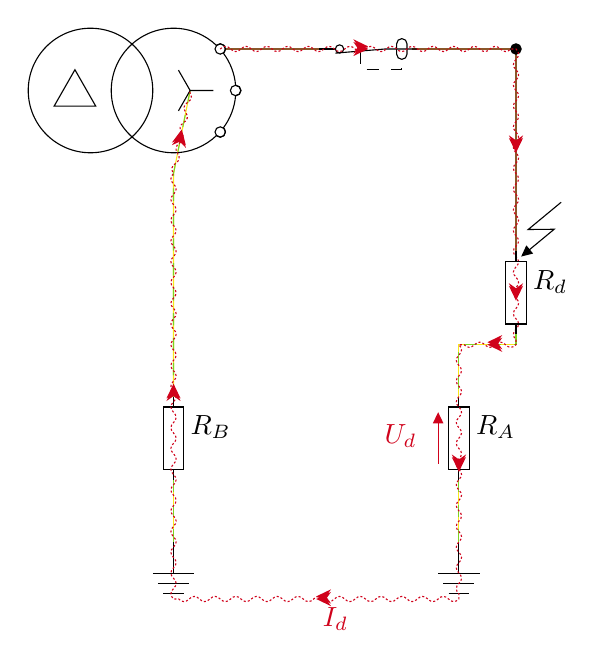
\begin{tikzpicture}[x=0.75pt,y=0.75pt,yscale=-1,xscale=1]
%uncomment if require: \path (0,353); %set diagram left start at 0, and has height of 353

%Straight Lines [id:da8450582290113836] 
\draw [color={rgb, 255:red, 248; green, 231; blue, 28 }  ,draw opacity=1 ]   (87.5,222.5) -- (87.5,252.5) ;
%Straight Lines [id:da035234150750507176] 
\draw [color={rgb, 255:red, 248; green, 231; blue, 28 }  ,draw opacity=1 ]   (252.5,152.5) -- (252.5,157.5) -- (225,157.5) -- (225,182.5) ;
%Straight Lines [id:da575921985906619] 
\draw [color={rgb, 255:red, 139; green, 87; blue, 42 }  ,draw opacity=1 ]   (112.5,15) -- (162.5,15) ;
%Straight Lines [id:da5726536295563455] 
\draw [color={rgb, 255:red, 248; green, 231; blue, 28 }  ,draw opacity=1 ]   (95.5,35) -- (87.5,75) -- (87.5,182.5) ;
%Straight Lines [id:da38476257001275427] 
\draw [color={rgb, 255:red, 126; green, 211; blue, 33 }  ,draw opacity=1 ] [dash pattern={on 4.5pt off 4.5pt}]  (95.5,35) -- (87.5,75) -- (87.5,182.5) ;
%Straight Lines [id:da9973940303994429] 
\draw [color={rgb, 255:red, 139; green, 87; blue, 42 }  ,draw opacity=1 ]   (202.5,15) -- (252.5,15) ;
%Shape: Path Data [id:dp9822778342813306] 
\draw   (112.5,55) .. controls (112.5,56.38) and (111.38,57.5) .. (110,57.5) .. controls (109.29,57.5) and (108.65,57.2) .. (108.19,56.72) .. controls (102.81,61.85) and (95.52,65) .. (87.5,65) .. controls (70.93,65) and (57.5,51.57) .. (57.5,35) .. controls (57.5,18.43) and (70.93,5) .. (87.5,5) .. controls (95.52,5) and (102.81,8.15) .. (108.19,13.28) .. controls (108.65,12.8) and (109.29,12.5) .. (110,12.5) .. controls (111.38,12.5) and (112.5,13.62) .. (112.5,15) .. controls (112.5,15.82) and (112.11,16.54) .. (111.5,17) .. controls (114.8,21.39) and (116.92,26.71) .. (117.4,32.5) .. controls (117.43,32.5) and (117.47,32.5) .. (117.5,32.5) .. controls (118.88,32.5) and (120,33.62) .. (120,35) .. controls (120,36.38) and (118.88,37.5) .. (117.5,37.5) .. controls (117.47,37.5) and (117.43,37.5) .. (117.4,37.5) .. controls (116.92,43.29) and (114.8,48.61) .. (111.5,53) .. controls (112.11,53.46) and (112.5,54.18) .. (112.5,55) -- cycle ;
%Shape: Circle [id:dp10169246549820965] 
\draw   (17.5,35) .. controls (17.5,18.43) and (30.93,5) .. (47.5,5) .. controls (64.07,5) and (77.5,18.43) .. (77.5,35) .. controls (77.5,51.57) and (64.07,65) .. (47.5,65) .. controls (30.93,65) and (17.5,51.57) .. (17.5,35) -- cycle ;
%Shape: Triangle [id:dp22185224755779764] 
\draw   (40,25) -- (30,42.5) -- (50,42.5) -- cycle ;
%Shape: Star [id:dp4535075510124722] 
\draw   (106.75,35) -- (95.5,35) -- (89.88,44.81) -- (95.5,35) -- (89.88,25.19) -- (95.5,35) -- cycle ;
%Shape: Circle [id:dp28187455970704567] 
\draw   (107.5,15) .. controls (107.5,13.62) and (108.62,12.5) .. (110,12.5) .. controls (111.38,12.5) and (112.5,13.62) .. (112.5,15) .. controls (112.5,16.38) and (111.38,17.5) .. (110,17.5) .. controls (108.62,17.5) and (107.5,16.38) .. (107.5,15) -- cycle ;
%Shape: Circle [id:dp9096244123377861] 
\draw   (114.9,35) .. controls (114.9,33.62) and (116.02,32.5) .. (117.4,32.5) .. controls (118.78,32.5) and (119.9,33.62) .. (119.9,35) .. controls (119.9,36.38) and (118.78,37.5) .. (117.4,37.5) .. controls (116.02,37.5) and (114.9,36.38) .. (114.9,35) -- cycle ;
%Shape: Circle [id:dp0660770114066822] 
\draw   (107.5,55) .. controls (107.5,53.62) and (108.62,52.5) .. (110,52.5) .. controls (111.38,52.5) and (112.5,53.62) .. (112.5,55) .. controls (112.5,56.38) and (111.38,57.5) .. (110,57.5) .. controls (108.62,57.5) and (107.5,56.38) .. (107.5,55) -- cycle ;

%Straight Lines [id:da12486709959480935] 
\draw [color={rgb, 255:red, 139; green, 87; blue, 42 }  ,draw opacity=1 ]   (252.5,112.5) -- (252.5,17.5) ;
%Straight Lines [id:da9194886303106931] 
\draw [color={rgb, 255:red, 126; green, 211; blue, 33 }  ,draw opacity=1 ] [dash pattern={on 4.5pt off 4.5pt}]  (252.5,152.5) -- (252.5,157.5) -- (225,157.5) -- (225,182.5) ;
%Straight Lines [id:da33889517147418446] 
\draw    (87.5,252.5) -- (87.5,267.5) ;
%Straight Lines [id:da7536356147270271] 
\draw    (77.5,267.5) -- (97.5,267.5) ;
%Straight Lines [id:da33790733335159795] 
\draw    (80,272.5) -- (95,272.5) ;
%Straight Lines [id:da8225336413065082] 
\draw    (82.5,277.5) -- (92.5,277.5) ;

%Straight Lines [id:da14728368722832463] 
\draw [color={rgb, 255:red, 126; green, 211; blue, 33 }  ,draw opacity=1 ] [dash pattern={on 4.5pt off 4.5pt}]  (87.5,222.5) -- (87.5,252.5) ;
%Straight Lines [id:da2713756434582886] 
\draw [color={rgb, 255:red, 248; green, 231; blue, 28 }  ,draw opacity=1 ]   (225,222.5) -- (225,252.5) ;
%Straight Lines [id:da07200185094723521] 
\draw    (225,252.5) -- (225,267.5) ;
%Straight Lines [id:da5503731135148442] 
\draw    (215,267.5) -- (235,267.5) ;
%Straight Lines [id:da9244125108161202] 
\draw    (217.5,272.5) -- (232.5,272.5) ;
%Straight Lines [id:da07512791048030887] 
\draw    (220,277.5) -- (230,277.5) ;

%Straight Lines [id:da5491926071123034] 
\draw [color={rgb, 255:red, 126; green, 211; blue, 33 }  ,draw opacity=1 ] [dash pattern={on 4.5pt off 4.5pt}]  (225,222.5) -- (225,252.5) ;
%Straight Lines [id:da7705666086878261] 
\draw    (87.5,217.5) -- (87.5,222.5) ;
%Shape: Rectangle [id:dp5724900932521552] 
\draw   (92.5,187.5) -- (92.5,217.5) -- (82.5,217.5) -- (82.5,187.5) -- cycle ;
%Straight Lines [id:da6857493814799358] 
\draw    (87.5,182.5) -- (87.5,187.5) ;

%Straight Lines [id:da7810225170823131] 
\draw    (225,217.5) -- (225,222.5) ;
%Shape: Rectangle [id:dp9839408028922504] 
\draw   (230,187.5) -- (230,217.5) -- (220,217.5) -- (220,187.5) -- cycle ;
%Straight Lines [id:da4367313473487816] 
\draw    (225,182.5) -- (225,187.5) ;

%Shape: Circle [id:dp6401617010113628] 
\draw  [fill={rgb, 255:red, 0; green, 0; blue, 0 }  ,fill opacity=1 ] (250,15) .. controls (250,13.62) and (251.12,12.5) .. (252.5,12.5) .. controls (253.88,12.5) and (255,13.62) .. (255,15) .. controls (255,16.38) and (253.88,17.5) .. (252.5,17.5) .. controls (251.12,17.5) and (250,16.38) .. (250,15) -- cycle ;
%Rounded Rect [id:dp9837999595449706] 
\draw   (197.5,20) .. controls (196.12,20) and (195,18.88) .. (195,17.5) -- (195,12.5) .. controls (195,11.12) and (196.12,10) .. (197.5,10) -- (197.5,10) .. controls (198.88,10) and (200,11.12) .. (200,12.5) -- (200,17.5) .. controls (200,18.88) and (198.88,20) .. (197.5,20) -- cycle ;
%Straight Lines [id:da04140906911364939] 
\draw  [dash pattern={on 4.5pt off 4.5pt}]  (177.5,16) -- (177.5,25) -- (197.5,25) -- (197.5,20) ;
%Shape: Circle [id:dp7012058816599942] 
\draw   (167.5,13) .. controls (166.4,13) and (165.5,13.9) .. (165.5,15) .. controls (165.5,16.1) and (166.4,17) .. (167.5,17) .. controls (168.6,17) and (169.5,16.1) .. (169.5,15) .. controls (169.5,13.9) and (168.6,13) .. (167.5,13) -- cycle ;
%Straight Lines [id:da23692932983683102] 
\draw    (165.5,15) -- (157.5,15) ;
%Straight Lines [id:da4567235518407359] 
\draw    (165.5,17) -- (189.5,15) -- (205,15) ;
%Shape: Boxed Line [id:dp44753967705251496] 
\draw    (274.27,88.83) -- (258.39,101.97) -- (270.89,101.86) -- (257.31,113.09) ;
\draw [shift={(255,115)}, rotate = 320.40999999999997] [fill={rgb, 255:red, 0; green, 0; blue, 0 }  ][line width=0.08]  [draw opacity=0] (5.36,-2.57) -- (0,0) -- (5.36,2.57) -- cycle    ;
\draw [color={rgb, 255:red, 208; green, 2; blue, 27 }  ,draw opacity=1 ] [dash pattern={on 0.75pt off 0.75pt}]  (110,15) .. controls (111.67,13.33) and (113.33,13.33) .. (115,15) .. controls (116.67,16.67) and (118.33,16.67) .. (120,15) .. controls (121.67,13.33) and (123.33,13.33) .. (125,15) .. controls (126.67,16.67) and (128.33,16.67) .. (130,15) .. controls (131.67,13.33) and (133.33,13.33) .. (135,15) .. controls (136.67,16.67) and (138.33,16.67) .. (140,15) .. controls (141.67,13.33) and (143.33,13.33) .. (145,15) .. controls (146.67,16.67) and (148.33,16.67) .. (150,15) .. controls (151.67,13.33) and (153.33,13.33) .. (155,15) .. controls (156.67,16.67) and (158.33,16.67) .. (160,15) .. controls (161.67,13.33) and (163.33,13.33) .. (165,15) .. controls (166.67,16.67) and (168.33,16.67) .. (170,15) .. controls (171.67,13.33) and (173.33,13.33) .. (175,15) .. controls (176.67,16.67) and (178.33,16.67) .. (180,15) .. controls (181.67,13.33) and (183.33,13.33) .. (185,15) .. controls (186.67,16.67) and (188.33,16.67) .. (190,15) .. controls (191.67,13.33) and (193.33,13.33) .. (195,15) .. controls (196.67,16.67) and (198.33,16.67) .. (200,15) .. controls (201.67,13.33) and (203.33,13.33) .. (205,15) .. controls (206.67,16.67) and (208.33,16.67) .. (210,15) .. controls (211.67,13.33) and (213.33,13.33) .. (215,15) .. controls (216.67,16.67) and (218.33,16.67) .. (220,15) .. controls (221.67,13.33) and (223.33,13.33) .. (225,15) .. controls (226.67,16.67) and (228.33,16.67) .. (230,15) .. controls (231.67,13.33) and (233.33,13.33) .. (235,15) .. controls (236.67,16.67) and (238.33,16.67) .. (240,15) .. controls (241.67,13.33) and (243.33,13.33) .. (245,15) .. controls (246.67,16.67) and (248.33,16.67) .. (250,15) -- (252.5,15) -- (252.5,15) .. controls (254.17,16.67) and (254.17,18.33) .. (252.5,20) .. controls (250.83,21.67) and (250.83,23.33) .. (252.5,25) .. controls (254.17,26.67) and (254.17,28.33) .. (252.5,30) .. controls (250.83,31.67) and (250.83,33.33) .. (252.5,35) .. controls (254.17,36.67) and (254.17,38.33) .. (252.5,40) .. controls (250.83,41.67) and (250.83,43.33) .. (252.5,45) .. controls (254.17,46.67) and (254.17,48.33) .. (252.5,50) .. controls (250.83,51.67) and (250.83,53.33) .. (252.5,55) .. controls (254.17,56.67) and (254.17,58.33) .. (252.5,60) .. controls (250.83,61.67) and (250.83,63.33) .. (252.5,65) .. controls (254.17,66.67) and (254.17,68.33) .. (252.5,70) .. controls (250.83,71.67) and (250.83,73.33) .. (252.5,75) .. controls (254.17,76.67) and (254.17,78.33) .. (252.5,80) .. controls (250.83,81.67) and (250.83,83.33) .. (252.5,85) .. controls (254.17,86.67) and (254.17,88.33) .. (252.5,90) .. controls (250.83,91.67) and (250.83,93.33) .. (252.5,95) .. controls (254.17,96.67) and (254.17,98.33) .. (252.5,100) .. controls (250.83,101.67) and (250.83,103.33) .. (252.5,105) .. controls (254.17,106.67) and (254.17,108.33) .. (252.5,110) .. controls (250.83,111.67) and (250.83,113.33) .. (252.5,115) -- (252.5,115) .. controls (254.17,116.67) and (254.17,118.33) .. (252.5,120) .. controls (250.83,121.67) and (250.83,123.33) .. (252.5,125) .. controls (254.17,126.67) and (254.17,128.33) .. (252.5,130) .. controls (250.83,131.67) and (250.83,133.33) .. (252.5,135) .. controls (254.17,136.67) and (254.17,138.33) .. (252.5,140) .. controls (250.83,141.67) and (250.83,143.33) .. (252.5,145) .. controls (254.17,146.67) and (254.17,148.33) .. (252.5,150) .. controls (250.83,151.67) and (250.83,153.33) .. (252.5,155) -- (252.5,157.5) -- (252.5,157.5) .. controls (250.83,159.17) and (249.17,159.17) .. (247.5,157.5) .. controls (245.83,155.83) and (244.17,155.83) .. (242.5,157.5) .. controls (240.83,159.17) and (239.17,159.17) .. (237.5,157.5) .. controls (235.83,155.83) and (234.17,155.83) .. (232.5,157.5) .. controls (230.83,159.17) and (229.17,159.17) .. (227.5,157.5) -- (225,157.5) -- (225,157.5) .. controls (226.67,159.17) and (226.67,160.83) .. (225,162.5) .. controls (223.33,164.17) and (223.33,165.83) .. (225,167.5) .. controls (226.67,169.17) and (226.67,170.83) .. (225,172.5) .. controls (223.33,174.17) and (223.33,175.83) .. (225,177.5) .. controls (226.67,179.17) and (226.67,180.83) .. (225,182.5) .. controls (223.33,184.17) and (223.33,185.83) .. (225,187.5) .. controls (226.67,189.17) and (226.67,190.83) .. (225,192.5) .. controls (223.33,194.17) and (223.33,195.83) .. (225,197.5) .. controls (226.67,199.17) and (226.67,200.83) .. (225,202.5) .. controls (223.33,204.17) and (223.33,205.83) .. (225,207.5) .. controls (226.67,209.17) and (226.67,210.83) .. (225,212.5) .. controls (223.33,214.17) and (223.33,215.83) .. (225,217.5) .. controls (226.67,219.17) and (226.67,220.83) .. (225,222.5) .. controls (223.33,224.17) and (223.33,225.83) .. (225,227.5) .. controls (226.67,229.17) and (226.67,230.83) .. (225,232.5) .. controls (223.33,234.17) and (223.33,235.83) .. (225,237.5) .. controls (226.67,239.17) and (226.67,240.83) .. (225,242.5) .. controls (223.33,244.17) and (223.33,245.83) .. (225,247.5) .. controls (226.67,249.17) and (226.67,250.83) .. (225,252.5) .. controls (223.33,254.17) and (223.33,255.83) .. (225,257.5) .. controls (226.67,259.17) and (226.67,260.83) .. (225,262.5) .. controls (223.33,264.17) and (223.33,265.83) .. (225,267.5) .. controls (226.67,269.17) and (226.67,270.83) .. (225,272.5) .. controls (223.33,274.17) and (223.33,275.83) .. (225,277.5) -- (225,280) -- (225,280) .. controls (223.33,281.67) and (221.67,281.67) .. (220,280) .. controls (218.33,278.33) and (216.67,278.33) .. (215,280) .. controls (213.33,281.67) and (211.67,281.67) .. (210,280) .. controls (208.33,278.33) and (206.67,278.33) .. (205,280) .. controls (203.33,281.67) and (201.67,281.67) .. (200,280) .. controls (198.33,278.33) and (196.67,278.33) .. (195,280) .. controls (193.33,281.67) and (191.67,281.67) .. (190,280) .. controls (188.33,278.33) and (186.67,278.33) .. (185,280) .. controls (183.33,281.67) and (181.67,281.67) .. (180,280) .. controls (178.33,278.33) and (176.67,278.33) .. (175,280) .. controls (173.33,281.67) and (171.67,281.67) .. (170,280) .. controls (168.33,278.33) and (166.67,278.33) .. (165,280) .. controls (163.33,281.67) and (161.67,281.67) .. (160,280) .. controls (158.33,278.33) and (156.67,278.33) .. (155,280) .. controls (153.33,281.67) and (151.67,281.67) .. (150,280) .. controls (148.33,278.33) and (146.67,278.33) .. (145,280) .. controls (143.33,281.67) and (141.67,281.67) .. (140,280) .. controls (138.33,278.33) and (136.67,278.33) .. (135,280) .. controls (133.33,281.67) and (131.67,281.67) .. (130,280) .. controls (128.33,278.33) and (126.67,278.33) .. (125,280) .. controls (123.33,281.67) and (121.67,281.67) .. (120,280) .. controls (118.33,278.33) and (116.67,278.33) .. (115,280) .. controls (113.33,281.67) and (111.67,281.67) .. (110,280) .. controls (108.33,278.33) and (106.67,278.33) .. (105,280) .. controls (103.33,281.67) and (101.67,281.67) .. (100,280) .. controls (98.33,278.33) and (96.67,278.33) .. (95,280) .. controls (93.33,281.67) and (91.67,281.67) .. (90,280) -- (87.5,280) -- (87.5,280) .. controls (85.83,278.33) and (85.83,276.67) .. (87.5,275) .. controls (89.17,273.33) and (89.17,271.67) .. (87.5,270) .. controls (85.83,268.33) and (85.83,266.67) .. (87.5,265) .. controls (89.17,263.33) and (89.17,261.67) .. (87.5,260) .. controls (85.83,258.33) and (85.83,256.67) .. (87.5,255) .. controls (89.17,253.33) and (89.17,251.67) .. (87.5,250) .. controls (85.83,248.33) and (85.83,246.67) .. (87.5,245) .. controls (89.17,243.33) and (89.17,241.67) .. (87.5,240) .. controls (85.83,238.33) and (85.83,236.67) .. (87.5,235) .. controls (89.17,233.33) and (89.17,231.67) .. (87.5,230) .. controls (85.83,228.33) and (85.83,226.67) .. (87.5,225) .. controls (89.17,223.33) and (89.17,221.67) .. (87.5,220) .. controls (85.83,218.33) and (85.83,216.67) .. (87.5,215) .. controls (89.17,213.33) and (89.17,211.67) .. (87.5,210) .. controls (85.83,208.33) and (85.83,206.67) .. (87.5,205) .. controls (89.17,203.33) and (89.17,201.67) .. (87.5,200) .. controls (85.83,198.33) and (85.83,196.67) .. (87.5,195) .. controls (89.17,193.33) and (89.17,191.67) .. (87.5,190) .. controls (85.83,188.33) and (85.83,186.67) .. (87.5,185) .. controls (89.17,183.33) and (89.17,181.67) .. (87.5,180) .. controls (85.83,178.33) and (85.83,176.67) .. (87.5,175) .. controls (89.17,173.33) and (89.17,171.67) .. (87.5,170) .. controls (85.83,168.33) and (85.83,166.67) .. (87.5,165) .. controls (89.17,163.33) and (89.17,161.67) .. (87.5,160) .. controls (85.83,158.33) and (85.83,156.67) .. (87.5,155) .. controls (89.17,153.33) and (89.17,151.67) .. (87.5,150) .. controls (85.83,148.33) and (85.83,146.67) .. (87.5,145) .. controls (89.17,143.33) and (89.17,141.67) .. (87.5,140) .. controls (85.83,138.33) and (85.83,136.67) .. (87.5,135) .. controls (89.17,133.33) and (89.17,131.67) .. (87.5,130) .. controls (85.83,128.33) and (85.83,126.67) .. (87.5,125) .. controls (89.17,123.33) and (89.17,121.67) .. (87.5,120) .. controls (85.83,118.33) and (85.83,116.67) .. (87.5,115) .. controls (89.17,113.33) and (89.17,111.67) .. (87.5,110) .. controls (85.83,108.33) and (85.83,106.67) .. (87.5,105) .. controls (89.17,103.33) and (89.17,101.67) .. (87.5,100) .. controls (85.83,98.33) and (85.83,96.67) .. (87.5,95) .. controls (89.17,93.33) and (89.17,91.67) .. (87.5,90) .. controls (85.83,88.33) and (85.83,86.67) .. (87.5,85) .. controls (89.17,83.33) and (89.17,81.67) .. (87.5,80) .. controls (85.83,78.33) and (85.83,76.67) .. (87.5,75) -- (87.5,75) .. controls (86.19,73.04) and (86.52,71.41) .. (88.48,70.1) .. controls (90.44,68.79) and (90.77,67.15) .. (89.46,65.19) .. controls (88.15,63.23) and (88.48,61.6) .. (90.44,60.29) .. controls (92.4,58.98) and (92.73,57.35) .. (91.42,55.39) .. controls (90.11,53.43) and (90.44,51.8) .. (92.4,50.49) .. controls (94.36,49.18) and (94.69,47.54) .. (93.38,45.58) .. controls (92.07,43.62) and (92.4,41.99) .. (94.36,40.68) .. controls (96.32,39.37) and (96.65,37.74) .. (95.34,35.78) -- (95.5,35) -- (95.5,35) ;
\draw [shift={(181.25,15)}, rotate = 180] [fill={rgb, 255:red, 208; green, 2; blue, 27 }  ,fill opacity=1 ][line width=0.08]  [draw opacity=0] (7.14,-3.43) -- (0,0) -- (7.14,3.43) -- (4.74,0) -- cycle    ;
\draw [shift={(252.5,65)}, rotate = 270] [fill={rgb, 255:red, 208; green, 2; blue, 27 }  ,fill opacity=1 ][line width=0.08]  [draw opacity=0] (7.14,-3.43) -- (0,0) -- (7.14,3.43) -- (4.74,0) -- cycle    ;
\draw [shift={(252.5,136.25)}, rotate = 270] [fill={rgb, 255:red, 208; green, 2; blue, 27 }  ,fill opacity=1 ][line width=0.08]  [draw opacity=0] (7.14,-3.43) -- (0,0) -- (7.14,3.43) -- (4.74,0) -- cycle    ;
\draw [shift={(238.75,157.5)}, rotate = 360] [fill={rgb, 255:red, 208; green, 2; blue, 27 }  ,fill opacity=1 ][line width=0.08]  [draw opacity=0] (7.14,-3.43) -- (0,0) -- (7.14,3.43) -- (4.74,0) -- cycle    ;
\draw [shift={(225,218.75)}, rotate = 270] [fill={rgb, 255:red, 208; green, 2; blue, 27 }  ,fill opacity=1 ][line width=0.08]  [draw opacity=0] (7.14,-3.43) -- (0,0) -- (7.14,3.43) -- (4.74,0) -- cycle    ;
\draw [shift={(156.25,280)}, rotate = 360] [fill={rgb, 255:red, 208; green, 2; blue, 27 }  ,fill opacity=1 ][line width=0.08]  [draw opacity=0] (7.14,-3.43) -- (0,0) -- (7.14,3.43) -- (4.74,0) -- cycle    ;
\draw [shift={(87.5,177.5)}, rotate = 450] [fill={rgb, 255:red, 208; green, 2; blue, 27 }  ,fill opacity=1 ][line width=0.08]  [draw opacity=0] (7.14,-3.43) -- (0,0) -- (7.14,3.43) -- (4.74,0) -- cycle    ;
\draw [shift={(91.5,55)}, rotate = 461.31] [fill={rgb, 255:red, 208; green, 2; blue, 27 }  ,fill opacity=1 ][line width=0.08]  [draw opacity=0] (7.14,-3.43) -- (0,0) -- (7.14,3.43) -- (4.74,0) -- cycle    ;
\draw [shift={(181.25,13.75)}, rotate = 180] [fill={rgb, 255:red, 208; green, 2; blue, 27 }  ,fill opacity=1 ][line width=0.08]  [draw opacity=0] (7.14,-3.43) -- (0,0) -- (7.14,3.43) -- (4.74,0) -- cycle    ;
\draw [shift={(252.5,63.75)}, rotate = 270] [fill={rgb, 255:red, 208; green, 2; blue, 27 }  ,fill opacity=1 ][line width=0.08]  [draw opacity=0] (7.14,-3.43) -- (0,0) -- (7.14,3.43) -- (4.74,0) -- cycle    ;
\draw [shift={(252.5,135)}, rotate = 270] [fill={rgb, 255:red, 208; green, 2; blue, 27 }  ,fill opacity=1 ][line width=0.08]  [draw opacity=0] (7.14,-3.43) -- (0,0) -- (7.14,3.43) -- (4.74,0) -- cycle    ;
\draw [shift={(238.75,156.25)}, rotate = 360] [fill={rgb, 255:red, 208; green, 2; blue, 27 }  ,fill opacity=1 ][line width=0.08]  [draw opacity=0] (7.14,-3.43) -- (0,0) -- (7.14,3.43) -- (4.74,0) -- cycle    ;
\draw [shift={(225,217.5)}, rotate = 270] [fill={rgb, 255:red, 208; green, 2; blue, 27 }  ,fill opacity=1 ][line width=0.08]  [draw opacity=0] (7.14,-3.43) -- (0,0) -- (7.14,3.43) -- (4.74,0) -- cycle    ;
\draw [shift={(156.25,278.75)}, rotate = 360] [fill={rgb, 255:red, 208; green, 2; blue, 27 }  ,fill opacity=1 ][line width=0.08]  [draw opacity=0] (7.14,-3.43) -- (0,0) -- (7.14,3.43) -- (4.74,0) -- cycle    ;
\draw [shift={(87.5,176.25)}, rotate = 450] [fill={rgb, 255:red, 208; green, 2; blue, 27 }  ,fill opacity=1 ][line width=0.08]  [draw opacity=0] (7.14,-3.43) -- (0,0) -- (7.14,3.43) -- (4.74,0) -- cycle    ;
\draw [shift={(91.5,53.75)}, rotate = 461.31] [fill={rgb, 255:red, 208; green, 2; blue, 27 }  ,fill opacity=1 ][line width=0.08]  [draw opacity=0] (7.14,-3.43) -- (0,0) -- (7.14,3.43) -- (4.74,0) -- cycle    ;
%Straight Lines [id:da9207949526828273] 
\draw    (252.5,147.5) -- (252.5,152.5) ;
%Shape: Rectangle [id:dp36210266951689685] 
\draw   (257.5,117.5) -- (257.5,147.5) -- (247.5,147.5) -- (247.5,117.5) -- cycle ;
%Straight Lines [id:da2843419817195654] 
\draw    (252.5,112.5) -- (252.5,117.5) ;

%Straight Lines [id:da667113945803525] 
\draw [color={rgb, 255:red, 208; green, 2; blue, 27 }  ,draw opacity=1 ]   (215,193) -- (215,215) ;
\draw [shift={(215,190)}, rotate = 90] [fill={rgb, 255:red, 208; green, 2; blue, 27 }  ,fill opacity=1 ][line width=0.08]  [draw opacity=0] (5.36,-2.57) -- (0,0) -- (5.36,2.57) -- cycle    ;

% Text Node
\draw (94.5,190.5) node [anchor=north west][inner sep=0.75pt]   [align=left] {$R_B$};
% Text Node
\draw (232,190.5) node [anchor=north west][inner sep=0.75pt]   [align=left] {$R_A$};
% Text Node
\draw (188,194.5) node [anchor=north west][inner sep=0.75pt]  [color={rgb, 255:red, 208; green, 2; blue, 27 }  ,opacity=1 ] [align=left] {$U_d$};
% Text Node
\draw (259.5,120.5) node [anchor=north west][inner sep=0.75pt]   [align=left] {$R_d$};
% Text Node
\draw (158.25,283) node [anchor=north west][inner sep=0.75pt] [color={rgb, 255:red, 208; green, 2; blue, 27 }]  [align=left] {$I_d$};


\end{tikzpicture}

\end{figure}

%\end{document}


\begin{comment}
\begin{circuitikz}[circuit ee IEC relay]
%\DrawGrid{(-1,-5)}{(9,3)} %grille d'aide pour le placement des objets

%alimentation

\node (D1) [make contact=point left, circuit breaker={point left}, tiny circuit symbols, activated] at (1,0.45) {};
\node (T1) [oosourcetransshape, prim=delta,sec=wye] at (0,0) {};


%neutre/terre

\node (RN) [R, label=$R_B$, rotate=90, tiny circuit symbols] at (0,-2.7) {};
\node (G1) [tlground] at (0,-3.9) {};
\draw [green!, thick] (G1) to node {} (RN) ; 
\draw [green!, thick] (RN) to (0,-0.5) to node {} (T1.sec4) ; 
\draw [dashed, yellow!, thick] (G1) to node {} (RN) ;
\draw [dashed, yellow!, thick] (RN) to (0,-0.5) to node {} (T1.sec4) ;

\node (RT) [resistor, rotate=90, tiny circuit symbols, label=$R_A$] at (2.5,-2.7) {};
\draw[-triangle 45, red] (2.8,-2) -- (2.8,-1) node[right,midway] {$U_d$};
\node (G2) [tlground] at (2.5,-3.9) {};
\draw [green!, thick] (RT) to (G2); 
\draw [dashed, yellow!, thick] (RT) to (G2);
\node (G2) [tlground] at (2.5,-3.9) {};
\draw [green!, thick] (G1) to (0,-4.2) to (2.5,-4.2) to (G2);
\draw [dashed, yellow!, thick] (G1) -- (0,-4.2) -- (2.5,-4.2) node [midway,below] {\color{black}$I_d$} -- (G2);
\node (G1) [tlground] at (0,-3.9) {};
\node (G2) [tlground] at (2.5,-3.9) {};

%appareil 1

\node (C2) [circ, scale=0.5] at (2.5,0.45) {};
\node (RD) [resistor, label=$R_d$, rotate=90, tiny circuit symbols] at (2.5,-1.5) {};

\draw [green!, thick] (RD) to (RT); 
\draw [dashed, yellow!, thick] (RD) to (RT); 

\draw [brown, thick] (T1.sec1) to (0.5,0.45) to (D1) to (C2) to (RD);
\node (T1) [oosourcetransshape, prim=delta,sec=wye] at (0,0) {};

%chemin courant

\fill [yellow!, decoration=lightning bolt, decorate] (2.5,-1.2) -- ++ (0.5,0.8); %éclairs
\path [postaction={on each segment={mid arrow=red}}]  (T1.sec1) -- (0.5,0.45) -- (D1) -- (C2) -- (RD) -- (RT) -- (G2) -- (2.5,-4.2) -- (1.666,-4.2) -- (0.88888,-4.2)  -- (0,-4.2) -- (G1) -- (RN) -- (0,-0.5) -- (T1.sec4); 

\callout{1,-0.5}{\cstep\label{pas:1}}{2.4,-1.2};


\end{circuitikz}
\end{comment}


L'intensité de courant $I_d$ vaut alors :
\begin{formule}[Courant de défaut $I_d$ en schéma TT]
\begin{align*}
		I_d &= \frac{U_{0}}{R_{B}+R_{A}+R_{d}}
\end{align*}
\end{formule}

\begin{textvariables}
U_{0}						& tension nominale simple						& volt			& \volt					& 	Différence de potentiel entre les masses métalliques et la terre 	\\
R_{B}						& résistance						& ohm			& \ohm					& 	Résistance de la prise de terre du neutre 	\\
R_{A}						& résistance						& ohm			& \ohm					& 	Résistance de la prise de terre de l'installation électrique 	\\
R_{d}						& résistance						& ohm			& \ohm					& 	Résistance de défaut 	d'isolement \\
\end{textvariables}

Le courant de défaut $I_d$ fera alors apparaître une \emph{tension de défaut} $U_d$ entre la masse métallique et la terre. Pour satisfaire aux normes de sécurité de la NF C15-100, il est imposé que la tension de défaut $U_d$ ne dépasse pas la tension de sécurité du local $U_L$ (voir \superref{subsec:prise_terre_installation_electrique}) :

\begin{formule}[Tension de défaut $U_d$ en schéma TT]
\begin{align*}
		U_d &= R_{A} \times I_{d} \\
			   &< U_L
\end{align*}
\end{formule}

\begin{textvariables}
R_{A}						& résistance						& ohm			& \ohm					& 	Résistance de la prise de terre de l'installation électrique 	\\
I_{d}							& intensité							& ampère		& \ampere				& 	Courant de défaut d'isolement \\
U_{L}						& tension							& volt			& \volt					& 	Tension de sécurité du local avec :
\begin{description}[nosep, leftmargin=*]
\item[Local sec :] $U_{L}=\SI{50}{\volt}$
\item[Local humide :] $U_{L}=\SI{25}{\volt}$
\end{description} \\
\end{textvariables}

Il est donc nécessaire de limiter $U_d$ à la valeur suivante (voir \superref{form:resistance_prise_terre}) :

\begin{formule}[Calibre du DDR $I_{\Delta n}$]
\begin{align*}
		I_{\Delta n} &< \frac{U_{L}}{R_{A}}
\end{align*}
\end{formule}

\begin{textvariables}
U_{L}						& tension							& volt			& \volt					& 	Tension de sécurité du local avec :
\begin{description}[nosep, leftmargin=*]
\item[Local sec :] $U_{L}=\SI{50}{\volt}$
\item[Local humide :] $U_{L}=\SI{25}{\volt}$
\end{description} \\
R_{A}						& résistance						& ohm			& \ohm					& 	Résistance de la prise de terre de l'installation électrique 	\\
\end{textvariables}

\begin{exemple}[Calcul du calibre du DDR $I_{\Delta n}$]
Si on considère que le transformateur est un transformateur $\SI{20}{\kilo\volt}/\SI{400}{\volt}$, que $R_A=\SI{20}{\ohm}$, que $R_B=\SI{10}{\ohm}$ et que $R_d$ est négligée, on peut déduire que le courant de défaut $I_d$ vaut :
\begin{align*}
		I_d 	&= \frac{U_{0}}{R_{B}+R_{A}} \\
				&=\frac{400}{20+10} \\
				&= \SI{13,33}{\ampere} \\
\end{align*}
Si une personne touche une masse des récepteurs en défaut, elle sera soumise à une tension de défaut $U_d$ :
\begin{align*}
		U_d 	&= R_{A} \times I_{d} \\
				&=20 \times 13,33 \\
				&= \SI{266,6}{\volt}
\end{align*}
La tension de défaut $U_d$ est dangereuse quelle que soit la tension limite choisie :
\begin{itemize}
\item coupure la plus rapide possible\,;
\item protection des personnes.
\end{itemize}
~\\
\begin{minipage}[t]{0.5\linewidth}
Dans le cas d'un local sec :
\begin{align*}
	I_{\Delta n} 	&< \frac{U_{L}}{R_{A}} \\
						&< \frac{50}{20} \\
						&< \SI{2,5}{\ampere}
\end{align*}
\end{minipage}
\hfill
\begin{minipage}[t]{0.5\linewidth}
Dans le cas d'un local humide :
\begin{align*}
	I_{\Delta n} 	&< \frac{U_{L}}{R_{A}} \\
						&< \frac{25}{20} \\
						&< \SI{1,25}{\ampere}
\end{align*}
\end{minipage}
~\\
D'après le tableau situé en \superref{tab:temps_coupure_DDR}, le DDR doit présenter un temps de coupure de moins de \SI{70}{\milli\second} avec une tension de défaut $U_d$ de \SI{266,6}{\volt} :

\begin{table}[h]
\begin{tabularx}{\linewidth}{X cccccccc}
\toprule
Tension nominale		& \multicolumn{2}{c}{$\SI{50}{\volt}<U_0\leq\SI{120}{\volt}$} 	& \multicolumn{2}{c}{$\SI{120}{\volt}<U_0\leq\SI{230}{\volt}$} & \multicolumn{2}{c}{$\SI{230}{\volt}<U_0\leq\SI{400}{\volt}$}		& \multicolumn{2}{c}{$U_0>\SI{400}{\volt}$}\\
\midrule
Type de courant		& alternatif	& continu	& alternatif	& continu	& alternatif	& continu	& alternatif	& continu \\
\addlinespace
Schéma TN/IT	& \SI{0,8}{\second}	&	\SI{5}{\second}	&	\SI{0,4}{\second}	&	\SI{5}{\second}	&	\SI{0,2}{\second}	&	\SI{0,4}{\second}	&	\SI{0,1}{\second}	&	\SI{0,1}{\second} \\	
\addlinespace
Schéma TT	& \SI{0,3}{\second}	&	\SI{5}{\second}	&	\SI{0,2}{\second}	&	\SI{0,4}{\second}	&	\cellcolor{green}\SI{0,07}{\second}	&	\SI{0,2}{\second}	&	\SI{0,04}{\second}	&	\SI{0,1}{\second} \\	
\bottomrule
\end{tabularx}
\end{table}
\end{exemple}

%\end{document}

	%--------------------------------------
%ELECTROTECHNIQUE - SCHEMA DE LIAISON A LA TERRE
%--------------------------------------

%utiliser les environnement \begin{comment} \end{comment} pour mettre en commentaire le préambule une fois la programmation appelée dans le document maître (!ne pas oublier de mettre en commentaire \end{document}!)

\begin{comment}

\documentclass[a4paper, 11pt, twoside, fleqn]{memoir}

\usepackage{AOCDTF}

\marqueurchapitre
\decoupagechapitre{1} %juste pour éviter les erreurs lors de la compilation des sous-programmations (passera en commentaire)

%--------------------------------------
%corps du document
%--------------------------------------

\begin{document} %corps du document
	\openleft %début de chapitre à gauche

\end{comment}

\chapter{Schéma Terre-Neutre\label{chap:schema_tn}}
\ChapFrame

\section{Caractéristiques générales}

\begin{definition}[Schéma TN]
Schéma de liaison à la terre dans lequel :
\begin{description}
\item[Neutre :] relié à la terre\,;
\item[Masses :] reliées au neutre du transformateur HT/BT.
\end{description}
\end{definition}

Dans le SLT TN, le point neutre du transformateur HT/BT (point commun) est relié à la terre via la \emph{prise de terre du neutre}. Cette liaison présente une certaine résistance, la \emph{résistance de la prise de terre du neutre} $R_B$. Sa mise en \oe{}uvre est à charge du fournisseur d'électricité et sa résistance globale doit être inférieure ou égale à \SI{15}{\ohm} \supercite{NF:C13-100-2015}.\\

Les masses sont quant à elles reliées au point neutre du transformateur HT/BT (point commun), cela peut être réalisé via trois déclinaisons du SLT TN :

%--------------------------------------
%ELECTROTECHNIQUE - SCHEMA DE LIAISON A LA TERRE
%--------------------------------------

%utiliser les environnement \begin{comment} \end{comment} pour mettre en commentaire le préambule une fois la programmation appelée dans le document maître (!ne pas oublier de mettre en commentaire \end{document}!)

%\begin{comment}

\documentclass[a4paper, 11pt, twoside, fleqn]{memoir}

\usepackage{AOCDTF}

\marqueurchapitre

%lien d'édition des figures Tikz sur le site mathcha.io (rajouter le lien d'une modification effectuée sur la figure tikz avec le nom du modificateur car il n'y a qu'un lien par compte)

%lien mathcha Nom Prénom : 

%--------------------------------------
%corps du document
%--------------------------------------

\begin{document} %corps du document
	\openleft %début de chapitre à gauche

%\end{comment}

\begin{landscape}

\begin{xltabular}{\textwidth}{c X X X c}
\caption{Déclinaisons du SLT TN}\\
\toprule
\thead{Nom}		& \thead{Caractéristiques}		& \thead{Avantages}		& \thead{Inconvénients} & \thead{Schéma sain} \\
\midrule
\endfirsthead %en-tête de la première page du tableau  
\multicolumn{5}{l}{\small\textit{Page précédente}} \\
\midrule %filet de milieu de tableau
\thead{Nom}		& \thead{Caractéristique}		& \thead{Schémas} 	& \thead{Inconvénients} 	& \thead{Schéma sain} \\
\midrule
\endhead
\midrule %filet de milieu de tableau
\multicolumn{5}{r}{\small\textit{Page suivante}} \\
\endfoot %pied de page de toutes les pages du tableau
\bottomrule
\endlastfoot %pied de page de la dernièredu tableau
Confondus (TN-C)		
& 
\begin{tabitemize}
\item Conducteurs neutre et PE confondus\,;
\item PE et neutre vert/jaune nommé conducteur Protection \'Equipotentielle Neutre (PEN)\,;
\item Connexion à la \emph{prise de terre du neutre} du poste HT/BT.
\end{tabitemize}
&
\begin{tabitemize}
\item économie d'un câble.
\end{tabitemize}
&		
\begin{tabitemize}
\item utilisation de canalisations fixes et rigides\,;
\item interdiction de pose :
	\begin{tabitemize}
	\item locaux à risques d'incendies\,;
	\item alimentation d'équipements de traitement de l'information (présence de courant harmonique dans le neutre).
	\end{tabitemize}
\end{tabitemize}	
& 
\adjustbox{valign=t}{\includepdf{fig_schema_tn-c_sain.pdf}}
\\

\end{xltabular}

\end{landscape}

\end{document}



Ce SLT présente les caractéristiques principales suivantes :
\begin{itemize}
\item utilisation uniquement dans les installations électriques alimentées par un transformateur HT/BT (ou MT/BT ou BT/BT)\,;
\item requiert l'installation de prises de terre uniformément réparties dans l'installation\,;
\item requiert la vérification des déclenchements sur le premier défaut d'isolement, obtenue lors de l'étude par des calculs de dimensionnement et, lors de la mise en service par des mesures de test\,; 
\item ne requiert pas de DDR dans l'absolu\,;
\item requiert un installateur qualifié pour toute installation, modification ou encore extension\,;
\item pouvant endommager de manière plus significative les bobinages et appareillages lors d'un défaut d'isolement, par rapport au SLT TT\,;
\item danger plus élevé dans les locaux à risque d'incendie du fait de courants de défaut plus importants.
\end{itemize}

\section{Schémas de principe}

\begin{figure}[H]
\caption{Installation Terre-Neutre Confondus}
\begin{subfigure}[t]{0.49\linewidth}
%--------------------------------------
%ELECTROTECHNIQUE - SCHEMA DE LIAISON A LA TERRE
%--------------------------------------

%utiliser les environnement \begin{comment} \end{comment} pour mettre en commentaire le préambule une fois la programmation appelée dans le document maître (!ne pas oublier de mettre en commentaire \end{document}!)

%\begin{comment}

\documentclass{standalone}

\usepackage{physics}
\usepackage{amsmath}
\usepackage{tikz}
\usepackage{mathdots}
\usepackage{yhmath}
\usepackage{cancel}
\usepackage{color}
\usepackage{siunitx}
\usepackage{array}
\usepackage{multirow}
\usepackage{amssymb}
\usepackage{gensymb}
\usepackage{tabularx}
\usepackage{booktabs}
\usetikzlibrary{fadings}
\usetikzlibrary{patterns}
\usetikzlibrary{shadows.blur}
\usetikzlibrary{shapes}

%lien d'édition des figures Tikz sur le site mathcha.io (rajouter le lien d'une modification effectuée sur la figure tikz avec le nom du modificateur car il n'y a qu'un lien par compte)

%lien mathcha Bruno Douchy : https://www.mathcha.io/editor/BkoJxFBDtnquyDl58vhj68k04ikMPoQOHQ2gjOW

%--------------------------------------
%corps du document
%--------------------------------------

\begin{document} %corps du document

%\end{comment}

% Pattern Info
 
\tikzset{
pattern size/.store in=\mcSize, 
pattern size = 5pt,
pattern thickness/.store in=\mcThickness, 
pattern thickness = 0.3pt,
pattern radius/.store in=\mcRadius, 
pattern radius = 1pt}
\makeatletter
\pgfutil@ifundefined{pgf@pattern@name@_bmmmws9wn}{
\pgfdeclarepatternformonly[\mcThickness,\mcSize]{_bmmmws9wn}
{\pgfqpoint{0pt}{0pt}}
{\pgfpoint{\mcSize+\mcThickness}{\mcSize+\mcThickness}}
{\pgfpoint{\mcSize}{\mcSize}}
{
\pgfsetcolor{\tikz@pattern@color}
\pgfsetlinewidth{\mcThickness}
\pgfpathmoveto{\pgfqpoint{0pt}{0pt}}
\pgfpathlineto{\pgfpoint{\mcSize+\mcThickness}{\mcSize+\mcThickness}}
\pgfusepath{stroke}
}}
\makeatother
\tikzset{every picture/.style={line width=0.5pt}} %set default line width to 0.75pt        

\begin{tikzpicture}[x=0.75pt,y=0.75pt,yscale=-0.5,xscale=0.5]
%uncomment if require: \path (0,293); %set diagram left start at 0, and has height of 293

%Straight Lines [id:da008483698413953467] 
\draw [color={rgb, 255:red, 248; green, 231; blue, 28 }  ,draw opacity=1 ]   (90,75) -- (460,75) ;
%Straight Lines [id:da06944587101382871] 
\draw [color={rgb, 255:red, 126; green, 211; blue, 33 }  ,draw opacity=1 ] [dash pattern={on 2.25pt off 2.25pt}]  (90,75) -- (460,75) ;
%Straight Lines [id:da7402424217268804] 
\draw [color={rgb, 255:red, 248; green, 231; blue, 28 }  ,draw opacity=1 ]   (87.5,222.5) -- (87.5,252.5) ;
%Straight Lines [id:da5918343393245601] 
\draw [color={rgb, 255:red, 248; green, 231; blue, 28 }  ,draw opacity=1 ]   (240,135) -- (225,135) -- (225,75) ;
%Straight Lines [id:da8855218059773354] 
\draw    (120,35) -- (162.5,35) ;
%Straight Lines [id:da4387311249705095] 
\draw [color={rgb, 255:red, 139; green, 87; blue, 42 }  ,draw opacity=1 ]   (112.5,15) -- (162.5,15) ;
%Straight Lines [id:da636953775291555] 
\draw [color={rgb, 255:red, 155; green, 155; blue, 155 }  ,draw opacity=1 ]   (112.5,55) -- (162.5,55) ;
%Straight Lines [id:da6725148311968068] 
\draw [color={rgb, 255:red, 248; green, 231; blue, 28 }  ,draw opacity=1 ]   (95.5,35) -- (87.5,75) -- (87.5,182.5) ;
%Straight Lines [id:da09238729671521517] 
\draw [color={rgb, 255:red, 126; green, 211; blue, 33 }  ,draw opacity=1 ] [dash pattern={on 2.25pt off 2.25pt}]  (95.5,35) -- (87.5,75) -- (87.5,182.5) ;
%Straight Lines [id:da8100957998136087] 
\draw    (202.5,35) -- (460,35) ;
%Straight Lines [id:da16093045358944136] 
\draw [color={rgb, 255:red, 139; green, 87; blue, 42 }  ,draw opacity=1 ]   (202.5,15) -- (460,15) ;
%Straight Lines [id:da20849694685551212] 
\draw [color={rgb, 255:red, 155; green, 155; blue, 155 }  ,draw opacity=1 ]   (202.5,55) -- (460,55) ;
%Shape: Path Data [id:dp6834291829337227] 
\draw   (112.5,55) .. controls (112.5,56.38) and (111.38,57.5) .. (110,57.5) .. controls (109.29,57.5) and (108.65,57.2) .. (108.19,56.72) .. controls (102.81,61.85) and (95.52,65) .. (87.5,65) .. controls (70.93,65) and (57.5,51.57) .. (57.5,35) .. controls (57.5,18.43) and (70.93,5) .. (87.5,5) .. controls (95.52,5) and (102.81,8.15) .. (108.19,13.28) .. controls (108.65,12.8) and (109.29,12.5) .. (110,12.5) .. controls (111.38,12.5) and (112.5,13.62) .. (112.5,15) .. controls (112.5,15.82) and (112.11,16.54) .. (111.5,17) .. controls (114.8,21.39) and (116.92,26.71) .. (117.4,32.5) .. controls (117.43,32.5) and (117.47,32.5) .. (117.5,32.5) .. controls (118.88,32.5) and (120,33.62) .. (120,35) .. controls (120,36.38) and (118.88,37.5) .. (117.5,37.5) .. controls (117.47,37.5) and (117.43,37.5) .. (117.4,37.5) .. controls (116.92,43.29) and (114.8,48.61) .. (111.5,53) .. controls (112.11,53.46) and (112.5,54.18) .. (112.5,55) -- cycle ;
%Shape: Circle [id:dp25520013984238377] 
\draw   (17.5,35) .. controls (17.5,18.43) and (30.93,5) .. (47.5,5) .. controls (64.07,5) and (77.5,18.43) .. (77.5,35) .. controls (77.5,51.57) and (64.07,65) .. (47.5,65) .. controls (30.93,65) and (17.5,51.57) .. (17.5,35) -- cycle ;
%Shape: Triangle [id:dp16879536749213853] 
\draw   (40,25) -- (30,42.5) -- (50,42.5) -- cycle ;
%Shape: Star [id:dp24745133775448547] 
\draw   (106.75,35) -- (95.5,35) -- (89.88,44.81) -- (95.5,35) -- (89.88,25.19) -- (95.5,35) -- cycle ;
%Shape: Circle [id:dp9864849188587985] 
\draw   (107.5,15) .. controls (107.5,13.62) and (108.62,12.5) .. (110,12.5) .. controls (111.38,12.5) and (112.5,13.62) .. (112.5,15) .. controls (112.5,16.38) and (111.38,17.5) .. (110,17.5) .. controls (108.62,17.5) and (107.5,16.38) .. (107.5,15) -- cycle ;
%Shape: Circle [id:dp03445318892672977] 
\draw   (114.9,35) .. controls (114.9,33.62) and (116.02,32.5) .. (117.4,32.5) .. controls (118.78,32.5) and (119.9,33.62) .. (119.9,35) .. controls (119.9,36.38) and (118.78,37.5) .. (117.4,37.5) .. controls (116.02,37.5) and (114.9,36.38) .. (114.9,35) -- cycle ;
%Shape: Circle [id:dp21435391141876436] 
\draw   (107.5,55) .. controls (107.5,53.62) and (108.62,52.5) .. (110,52.5) .. controls (111.38,52.5) and (112.5,53.62) .. (112.5,55) .. controls (112.5,56.38) and (111.38,57.5) .. (110,57.5) .. controls (108.62,57.5) and (107.5,56.38) .. (107.5,55) -- cycle ;

%Straight Lines [id:da9414980338893979] 
\draw [color={rgb, 255:red, 74; green, 144; blue, 226 }  ,draw opacity=1 ]   (292.5,112.5) -- (292.5,77.5) ;
%Straight Lines [id:da27751530095615806] 
\draw [color={rgb, 255:red, 139; green, 87; blue, 42 }  ,draw opacity=1 ]   (252.5,112.5) -- (252.5,17.5) ;
%Straight Lines [id:da8401783030061442] 
\draw [color={rgb, 255:red, 139; green, 87; blue, 42 }  ,draw opacity=1 ]   (252.5,130) -- (252.5,117.5) ;
%Straight Lines [id:da6144198142388259] 
\draw [color={rgb, 255:red, 74; green, 144; blue, 226 }  ,draw opacity=1 ]   (292.5,130.5) -- (292.5,117.5) ;
%Straight Lines [id:da08447178364240893] 
\draw    (45,232.5) -- (460,232.5) ;
%Shape: Rectangle [id:dp6917865548447948] 
\draw  [draw opacity=0][pattern=_bmmmws9wn,pattern size=6pt,pattern thickness=0.75pt,pattern radius=0pt, pattern color={rgb, 255:red, 0; green, 0; blue, 0}][line width=0.75]  (45,232.5) -- (460,232.5) -- (460,247.5) -- (45,247.5) -- cycle ;
%Straight Lines [id:da5758120659627904] 
\draw [color={rgb, 255:red, 126; green, 211; blue, 33 }  ,draw opacity=1 ] [dash pattern={on 2.25pt off 2.25pt}]  (240,135) -- (225,135) -- (225,75) ;
%Straight Lines [id:da3042650335499705] 
\draw    (87.5,252.5) -- (87.5,267.5) ;
%Straight Lines [id:da5819552828178339] 
\draw    (77.5,267.5) -- (97.5,267.5) ;
%Straight Lines [id:da5191842943668726] 
\draw    (80,272.5) -- (95,272.5) ;
%Straight Lines [id:da20267125061533042] 
\draw    (82.5,277.5) -- (92.5,277.5) ;

%Straight Lines [id:da1731291153518706] 
\draw [color={rgb, 255:red, 126; green, 211; blue, 33 }  ,draw opacity=1 ] [dash pattern={on 2.25pt off 2.25pt}]  (87.5,222.5) -- (87.5,252.5) ;
%Straight Lines [id:da447845422109466] 
\draw    (287.5,130) -- (292.5,130) ;
%Shape: Rectangle [id:dp520581263360185] 
\draw   (257.5,125) -- (287.5,125) -- (287.5,135) -- (257.5,135) -- cycle ;
%Straight Lines [id:da5356387601329091] 
\draw    (252.5,130) -- (257.5,130) ;

%Straight Lines [id:da07643260567103483] 
\draw    (87.5,217.5) -- (87.5,222.5) ;
%Shape: Rectangle [id:dp008342316051101917] 
\draw   (92.5,187.5) -- (92.5,217.5) -- (82.5,217.5) -- (82.5,187.5) -- cycle ;
%Straight Lines [id:da09697746232408333] 
\draw    (87.5,182.5) -- (87.5,187.5) ;

%Straight Lines [id:da1742958722449034] 
\draw [color={rgb, 255:red, 248; green, 231; blue, 28 }  ,draw opacity=1 ]   (325,135) -- (310,135) -- (310,75) ;
%Straight Lines [id:da016656189472749827] 
\draw [color={rgb, 255:red, 74; green, 144; blue, 226 }  ,draw opacity=1 ]   (377.5,112.5) -- (377.5,77.5) ;
%Straight Lines [id:da09528364052879534] 
\draw [color={rgb, 255:red, 139; green, 87; blue, 42 }  ,draw opacity=1 ]   (337.5,112.5) -- (337.5,17.5) ;
%Straight Lines [id:da31579551999326805] 
\draw [color={rgb, 255:red, 139; green, 87; blue, 42 }  ,draw opacity=1 ]   (337.5,130) -- (337.5,117.5) ;
%Straight Lines [id:da8299851447706146] 
\draw [color={rgb, 255:red, 74; green, 144; blue, 226 }  ,draw opacity=1 ]   (377.5,130.5) -- (377.5,117.5) ;
%Straight Lines [id:da33732409899195637] 
\draw [color={rgb, 255:red, 126; green, 211; blue, 33 }  ,draw opacity=1 ] [dash pattern={on 2.25pt off 2.25pt}]  (325,135) -- (310,135) -- (310,75) ;
%Straight Lines [id:da44333407130344615] 
\draw    (372.5,130) -- (377.5,130) ;
%Shape: Rectangle [id:dp8912988160440456] 
\draw   (342.5,125) -- (372.5,125) -- (372.5,135) -- (342.5,135) -- cycle ;
%Straight Lines [id:da6881533641386929] 
\draw    (337.5,130) -- (342.5,130) ;

%Straight Lines [id:da9265870438738062] 
\draw [color={rgb, 255:red, 248; green, 231; blue, 28 }  ,draw opacity=1 ]   (410,135) -- (395,135) -- (395,75) ;
%Straight Lines [id:da29888425275861696] 
\draw [color={rgb, 255:red, 74; green, 144; blue, 226 }  ,draw opacity=1 ]   (462.5,112.5) -- (462.5,77.5) ;
%Straight Lines [id:da19160803833752127] 
\draw [color={rgb, 255:red, 139; green, 87; blue, 42 }  ,draw opacity=1 ]   (422.5,112.5) -- (422.5,17.5) ;
%Straight Lines [id:da2386502061815522] 
\draw [color={rgb, 255:red, 139; green, 87; blue, 42 }  ,draw opacity=1 ]   (422.5,130) -- (422.5,117.5) ;
%Straight Lines [id:da8099974104215516] 
\draw [color={rgb, 255:red, 74; green, 144; blue, 226 }  ,draw opacity=1 ]   (462.5,130.5) -- (462.5,117.5) ;
%Straight Lines [id:da5974904676194153] 
\draw [color={rgb, 255:red, 126; green, 211; blue, 33 }  ,draw opacity=1 ] [dash pattern={on 2.25pt off 2.25pt}]  (410,135) -- (395,135) -- (395,75) ;
%Straight Lines [id:da24571432228663814] 
\draw    (457.5,130) -- (462.5,130) ;
%Shape: Rectangle [id:dp7341042129075479] 
\draw   (427.5,125) -- (457.5,125) -- (457.5,135) -- (427.5,135) -- cycle ;
%Straight Lines [id:da8263877672394346] 
\draw    (422.5,130) -- (427.5,130) ;

%Shape: Circle [id:dp7480136730647264] 
\draw  [fill={rgb, 255:red, 0; green, 0; blue, 0 }  ,fill opacity=1 ] (375,75) .. controls (375,73.62) and (376.12,72.5) .. (377.5,72.5) .. controls (378.88,72.5) and (380,73.62) .. (380,75) .. controls (380,76.38) and (378.88,77.5) .. (377.5,77.5) .. controls (376.12,77.5) and (375,76.38) .. (375,75) -- cycle ;
%Shape: Circle [id:dp20106995777905023] 
\draw  [fill={rgb, 255:red, 0; green, 0; blue, 0 }  ,fill opacity=1 ] (460,75) .. controls (460,73.62) and (461.12,72.5) .. (462.5,72.5) .. controls (463.88,72.5) and (465,73.62) .. (465,75) .. controls (465,76.38) and (463.88,77.5) .. (462.5,77.5) .. controls (461.12,77.5) and (460,76.38) .. (460,75) -- cycle ;
%Shape: Circle [id:dp30375287231255577] 
\draw  [fill={rgb, 255:red, 0; green, 0; blue, 0 }  ,fill opacity=1 ] (335,15) .. controls (335,13.62) and (336.12,12.5) .. (337.5,12.5) .. controls (338.88,12.5) and (340,13.62) .. (340,15) .. controls (340,16.38) and (338.88,17.5) .. (337.5,17.5) .. controls (336.12,17.5) and (335,16.38) .. (335,15) -- cycle ;
%Shape: Circle [id:dp1979307718008253] 
\draw  [fill={rgb, 255:red, 0; green, 0; blue, 0 }  ,fill opacity=1 ] (420,15) .. controls (420,13.62) and (421.12,12.5) .. (422.5,12.5) .. controls (423.88,12.5) and (425,13.62) .. (425,15) .. controls (425,16.38) and (423.88,17.5) .. (422.5,17.5) .. controls (421.12,17.5) and (420,16.38) .. (420,15) -- cycle ;
%Shape: Circle [id:dp08277262683691078] 
\draw  [fill={rgb, 255:red, 0; green, 0; blue, 0 }  ,fill opacity=1 ] (290,75) .. controls (290,73.62) and (291.12,72.5) .. (292.5,72.5) .. controls (293.88,72.5) and (295,73.62) .. (295,75) .. controls (295,76.38) and (293.88,77.5) .. (292.5,77.5) .. controls (291.12,77.5) and (290,76.38) .. (290,75) -- cycle ;
%Shape: Circle [id:dp2507630610609335] 
\draw  [fill={rgb, 255:red, 0; green, 0; blue, 0 }  ,fill opacity=1 ] (250,15) .. controls (250,13.62) and (251.12,12.5) .. (252.5,12.5) .. controls (253.88,12.5) and (255,13.62) .. (255,15) .. controls (255,16.38) and (253.88,17.5) .. (252.5,17.5) .. controls (251.12,17.5) and (250,16.38) .. (250,15) -- cycle ;
%Straight Lines [id:da6877054516361302] 
%\draw    (70,152.5) -- (81.83,185.62) ;
%\draw [shift={(82.5,187.5)}, rotate = 250.35] [color={rgb, 255:red, 0; green, 0; blue, 0 }  ][line width=0.75]    (10.93,-3.29) .. controls (6.95,-1.4) and (3.31,-0.3) .. (0,0) .. controls (3.31,0.3) and (6.95,1.4) .. (10.93,3.29)   ;
%Straight Lines [id:da6269819660832152] 
%\draw    (142.5,212.5) -- (96.38,261.05) ;
%\draw [shift={(95,262.5)}, rotate = 313.53] [color={rgb, 255:red, 0; green, 0; blue, 0 }  ][line width=0.75]    (10.93,-3.29) .. controls (6.95,-1.4) and (3.31,-0.3) .. (0,0) .. controls (3.31,0.3) and (6.95,1.4) .. (10.93,3.29)   ;
%Shape: Rectangle [id:dp19008190111612866] 
\draw  [dash pattern={on 2.25pt off 2.25pt on 1pt off 2.25pt}] (242.5,115) -- (302.5,115) -- (302.5,145) -- (242.5,145) -- cycle ;
%Shape: Circle [id:dp22840916642995968] 
\draw  [fill={rgb, 255:red, 255; green, 255; blue, 255 }  ,fill opacity=1 ] (240,135) .. controls (240,133.62) and (241.12,132.5) .. (242.5,132.5) .. controls (243.88,132.5) and (245,133.62) .. (245,135) .. controls (245,136.38) and (243.88,137.5) .. (242.5,137.5) .. controls (241.12,137.5) and (240,136.38) .. (240,135) -- cycle ;
%Shape: Circle [id:dp8394579201908906] 
\draw  [fill={rgb, 255:red, 255; green, 255; blue, 255 }  ,fill opacity=1 ] (250,115) .. controls (250,113.62) and (251.12,112.5) .. (252.5,112.5) .. controls (253.88,112.5) and (255,113.62) .. (255,115) .. controls (255,116.38) and (253.88,117.5) .. (252.5,117.5) .. controls (251.12,117.5) and (250,116.38) .. (250,115) -- cycle ;
%Shape: Circle [id:dp59120282818972] 
\draw  [fill={rgb, 255:red, 255; green, 255; blue, 255 }  ,fill opacity=1 ] (290,115) .. controls (290,113.62) and (291.12,112.5) .. (292.5,112.5) .. controls (293.88,112.5) and (295,113.62) .. (295,115) .. controls (295,116.38) and (293.88,117.5) .. (292.5,117.5) .. controls (291.12,117.5) and (290,116.38) .. (290,115) -- cycle ;
%Shape: Rectangle [id:dp6441734419109765] 
\draw  [dash pattern={on 2.25pt off 2.25pt on 1pt off 2.25pt}] (327.5,115) -- (387.5,115) -- (387.5,145) -- (327.5,145) -- cycle ;
%Shape: Circle [id:dp31127955764480597] 
\draw  [fill={rgb, 255:red, 255; green, 255; blue, 255 }  ,fill opacity=1 ] (325,135) .. controls (325,133.62) and (326.12,132.5) .. (327.5,132.5) .. controls (328.88,132.5) and (330,133.62) .. (330,135) .. controls (330,136.38) and (328.88,137.5) .. (327.5,137.5) .. controls (326.12,137.5) and (325,136.38) .. (325,135) -- cycle ;
%Shape: Circle [id:dp19213098942989493] 
\draw  [fill={rgb, 255:red, 255; green, 255; blue, 255 }  ,fill opacity=1 ] (335,115) .. controls (335,113.62) and (336.12,112.5) .. (337.5,112.5) .. controls (338.88,112.5) and (340,113.62) .. (340,115) .. controls (340,116.38) and (338.88,117.5) .. (337.5,117.5) .. controls (336.12,117.5) and (335,116.38) .. (335,115) -- cycle ;
%Shape: Circle [id:dp6404787749234091] 
\draw  [fill={rgb, 255:red, 255; green, 255; blue, 255 }  ,fill opacity=1 ] (375,115) .. controls (375,113.62) and (376.12,112.5) .. (377.5,112.5) .. controls (378.88,112.5) and (380,113.62) .. (380,115) .. controls (380,116.38) and (378.88,117.5) .. (377.5,117.5) .. controls (376.12,117.5) and (375,116.38) .. (375,115) -- cycle ;
%Shape: Rectangle [id:dp557242515638855] 
\draw  [dash pattern={on 2.25pt off 2.25pt on 1pt off 2.25pt}] (412.5,115) -- (472.5,115) -- (472.5,145) -- (412.5,145) -- cycle ;
%Shape: Circle [id:dp29406753228301175] 
\draw  [fill={rgb, 255:red, 255; green, 255; blue, 255 }  ,fill opacity=1 ] (410,135) .. controls (410,133.62) and (411.12,132.5) .. (412.5,132.5) .. controls (413.88,132.5) and (415,133.62) .. (415,135) .. controls (415,136.38) and (413.88,137.5) .. (412.5,137.5) .. controls (411.12,137.5) and (410,136.38) .. (410,135) -- cycle ;
%Shape: Circle [id:dp7457639592130139] 
\draw  [fill={rgb, 255:red, 255; green, 255; blue, 255 }  ,fill opacity=1 ] (420,115) .. controls (420,113.62) and (421.12,112.5) .. (422.5,112.5) .. controls (423.88,112.5) and (425,113.62) .. (425,115) .. controls (425,116.38) and (423.88,117.5) .. (422.5,117.5) .. controls (421.12,117.5) and (420,116.38) .. (420,115) -- cycle ;
%Shape: Circle [id:dp7096093119796795] 
\draw  [fill={rgb, 255:red, 255; green, 255; blue, 255 }  ,fill opacity=1 ] (460,115) .. controls (460,113.62) and (461.12,112.5) .. (462.5,112.5) .. controls (463.88,112.5) and (465,113.62) .. (465,115) .. controls (465,116.38) and (463.88,117.5) .. (462.5,117.5) .. controls (461.12,117.5) and (460,116.38) .. (460,115) -- cycle ;
%Shape: Circle [id:dp7560227930994274] 
\draw  [fill={rgb, 255:red, 0; green, 0; blue, 0 }  ,fill opacity=1 ] (222.5,75) .. controls (222.5,73.62) and (223.62,72.5) .. (225,72.5) .. controls (226.38,72.5) and (227.5,73.62) .. (227.5,75) .. controls (227.5,76.38) and (226.38,77.5) .. (225,77.5) .. controls (223.62,77.5) and (222.5,76.38) .. (222.5,75) -- cycle ;
%Shape: Circle [id:dp5992483948938637] 
\draw  [fill={rgb, 255:red, 0; green, 0; blue, 0 }  ,fill opacity=1 ] (307.5,75) .. controls (307.5,73.62) and (308.62,72.5) .. (310,72.5) .. controls (311.38,72.5) and (312.5,73.62) .. (312.5,75) .. controls (312.5,76.38) and (311.38,77.5) .. (310,77.5) .. controls (308.62,77.5) and (307.5,76.38) .. (307.5,75) -- cycle ;
%Shape: Circle [id:dp69556176770618] 
\draw  [fill={rgb, 255:red, 0; green, 0; blue, 0 }  ,fill opacity=1 ] (392.5,75) .. controls (392.5,73.62) and (393.62,72.5) .. (395,72.5) .. controls (396.38,72.5) and (397.5,73.62) .. (397.5,75) .. controls (397.5,76.38) and (396.38,77.5) .. (395,77.5) .. controls (393.62,77.5) and (392.5,76.38) .. (392.5,75) -- cycle ;
%Shape: Circle [id:dp8403502042750037] 
\draw  [fill={rgb, 255:red, 0; green, 0; blue, 0 }  ,fill opacity=1 ] (85,75) .. controls (85,73.62) and (86.12,72.5) .. (87.5,72.5) .. controls (88.88,72.5) and (90,73.62) .. (90,75) .. controls (90,76.38) and (88.88,77.5) .. (87.5,77.5) .. controls (86.12,77.5) and (85,76.38) .. (85,75) -- cycle ;
%Straight Lines [id:da7681307281422329] 
\draw    (170,67.5) -- (192.5,55) -- (202.5,55) ;
%Straight Lines [id:da13712476034717958] 
\draw    (170,47.5) -- (192.5,35) -- (202.5,35) ;
%Straight Lines [id:da830167108509327] 
\draw  [dash pattern={on 2.25pt off 2.25pt}]  (181.25,61.25) -- (181.25,21.25) ;
%Straight Lines [id:da5425144082331462] 
\draw    (170,27.5) -- (192.5,15) -- (202.5,15) ;
%Straight Lines [id:da14338828534258663] 
\draw    (172.5,55) -- (162.5,55) ;
\draw [shift={(172.5,55)}, rotate = 225] [color={rgb, 255:red, 0; green, 0; blue, 0 }  ][line width=0.75]    (-3.35,0) -- (3.35,0)(0,3.35) -- (0,-3.35)   ;
%Straight Lines [id:da018968623053294387] 
\draw    (172.5,35) -- (162.5,35) ;
\draw [shift={(172.5,35)}, rotate = 225] [color={rgb, 255:red, 0; green, 0; blue, 0 }  ][line width=0.75]    (-3.35,0) -- (3.35,0)(0,3.35) -- (0,-3.35)   ;
%Straight Lines [id:da7549515123527469] 
\draw    (172.5,15) -- (162.5,15) ;
\draw [shift={(172.5,15)}, rotate = 225] [color={rgb, 255:red, 0; green, 0; blue, 0 }  ][line width=0.75]    (-3.35,0) -- (3.35,0)(0,3.35) -- (0,-3.35)   ;

% Text Node
%\draw (94.5,190.5) node [anchor=north west][inner sep=0.75pt]   [align=left] {$R_b$};
% Text Node
%\draw (55,124) node [anchor=north west][inner sep=0.75pt]   [align=left] {\Circled{2}};
% Text Node
%\draw (130,186) node [anchor=north west][inner sep=0.75pt]   [align=left] {\Circled{1}};
% Text Node
%\draw (294.5,93) node [anchor=north west][inner sep=0.75pt]   [align=left] {1};
% Text Node
%\draw (379.5,93) node [anchor=north west][inner sep=0.75pt]   [align=left] {2};
% Text Node
%\draw (464.5,93) node [anchor=north west][inner sep=0.75pt]   [align=left] {3};


\end{tikzpicture}

\end{document}
\subcaption{sans défaut d'isolement}
\end{subfigure}
\begin{subfigure}[t]{0.49\linewidth}
%--------------------------------------
%ELECTROTECHNIQUE - SCHEMA DE LIAISON A LA TERRE
%--------------------------------------

%utiliser les environnement \begin{comment} \end{comment} pour mettre en commentaire le préambule une fois la programmation appelée dans le document maître (!ne pas oublier de mettre en commentaire \end{document}!)

\begin{comment}

\documentclass[a4paper, 11pt, twoside, fleqn]{memoir}

\usepackage{AOCDTF}

\marqueurchapitre

%lien d'édition des figures Tikz sur le site mathcha.io (rajouter le lien d'une modification effectuée sur la figure tikz avec le nom du modificateur car il n'y a qu'un lien par compte)

%lien mathcha Bruno Douchy : https://www.mathcha.io/editor/lOZOZtPztP7tJld2nWSOen4oyF3ZLzN2Sj62Pv

%--------------------------------------
%corps du document
%--------------------------------------

\begin{document} %corps du document
	\openleft %début de chapitre à gauche

\end{comment}



% Pattern Info
 
\tikzset{
pattern size/.store in=\mcSize, 
pattern size = 5pt,
pattern thickness/.store in=\mcThickness, 
pattern thickness = 0.3pt,
pattern radius/.store in=\mcRadius, 
pattern radius = 1pt}
\makeatletter
\pgfutil@ifundefined{pgf@pattern@name@_mntx1d0th}{
\pgfdeclarepatternformonly[\mcThickness,\mcSize]{_mntx1d0th}
{\pgfqpoint{0pt}{0pt}}
{\pgfpoint{\mcSize+\mcThickness}{\mcSize+\mcThickness}}
{\pgfpoint{\mcSize}{\mcSize}}
{
\pgfsetcolor{\tikz@pattern@color}
\pgfsetlinewidth{\mcThickness}
\pgfpathmoveto{\pgfqpoint{0pt}{0pt}}
\pgfpathlineto{\pgfpoint{\mcSize+\mcThickness}{\mcSize+\mcThickness}}
\pgfusepath{stroke}
}}
\makeatother
\tikzset{every picture/.style={line width=0.5pt}} %set default line width to 0.75pt        

\begin{tikzpicture}[x=0.75pt,y=0.75pt,yscale=-0.6,xscale=0.6]
%uncomment if require: \path (0,235); %set diagram left start at 0, and has height of 235

%Straight Lines [id:da8171558078184873] 
\draw [color={rgb, 255:red, 248; green, 231; blue, 28 }  ,draw opacity=1 ]   (90,75) -- (460,75) ;
%Straight Lines [id:da16438907305411632] 
\draw [color={rgb, 255:red, 126; green, 211; blue, 33 }  ,draw opacity=1 ] [dash pattern={on 2.25pt off 2.25pt}]  (90,75) -- (460,75) ;
%Straight Lines [id:da3591349784222725] 
\draw [color={rgb, 255:red, 248; green, 231; blue, 28 }  ,draw opacity=1 ]   (87.5,162.5) -- (87.5,192.5) ;
%Straight Lines [id:da008765067779469726] 
\draw [color={rgb, 255:red, 248; green, 231; blue, 28 }  ,draw opacity=1 ]   (240,135) -- (225,135) -- (225,75) ;
%Straight Lines [id:da9996152121194258] 
\draw    (120,35) -- (162.5,35) ;
%Straight Lines [id:da5023751395172481] 
\draw [color={rgb, 255:red, 139; green, 87; blue, 42 }  ,draw opacity=1 ]   (112.5,15) -- (162.5,15) ;
%Straight Lines [id:da6629450629275421] 
\draw [color={rgb, 255:red, 155; green, 155; blue, 155 }  ,draw opacity=1 ]   (112.5,55) -- (162.5,55) ;
%Straight Lines [id:da7406348808045065] 
\draw [color={rgb, 255:red, 248; green, 231; blue, 28 }  ,draw opacity=1 ]   (95.5,35) -- (87.5,75) -- (87.5,122.5) ;
%Straight Lines [id:da8967520631020585] 
\draw [color={rgb, 255:red, 126; green, 211; blue, 33 }  ,draw opacity=1 ] [dash pattern={on 2.25pt off 2.25pt}]  (95.5,35) -- (87.5,75) -- (87.5,122.5) ;
%Shape: Circle [id:dp0027818785253741485] 
\draw  [fill={rgb, 255:red, 0; green, 0; blue, 0 }  ,fill opacity=1 ] (85,75) .. controls (85,73.62) and (86.12,72.5) .. (87.5,72.5) .. controls (88.88,72.5) and (90,73.62) .. (90,75) .. controls (90,76.38) and (88.88,77.5) .. (87.5,77.5) .. controls (86.12,77.5) and (85,76.38) .. (85,75) -- cycle ;
%Straight Lines [id:da5752741404016657] 
\draw    (202.5,35) -- (460,35) ;
%Straight Lines [id:da4814004273751151] 
\draw [color={rgb, 255:red, 139; green, 87; blue, 42 }  ,draw opacity=1 ]   (202.5,15) -- (460,15) ;
%Straight Lines [id:da3315148063986225] 
\draw [color={rgb, 255:red, 155; green, 155; blue, 155 }  ,draw opacity=1 ]   (202.5,55) -- (460,55) ;
%Shape: Path Data [id:dp897526939895229] 
\draw   (112.5,55) .. controls (112.5,56.38) and (111.38,57.5) .. (110,57.5) .. controls (109.29,57.5) and (108.65,57.2) .. (108.19,56.72) .. controls (102.81,61.85) and (95.52,65) .. (87.5,65) .. controls (70.93,65) and (57.5,51.57) .. (57.5,35) .. controls (57.5,18.43) and (70.93,5) .. (87.5,5) .. controls (95.52,5) and (102.81,8.15) .. (108.19,13.28) .. controls (108.65,12.8) and (109.29,12.5) .. (110,12.5) .. controls (111.38,12.5) and (112.5,13.62) .. (112.5,15) .. controls (112.5,15.82) and (112.11,16.54) .. (111.5,17) .. controls (114.8,21.39) and (116.92,26.71) .. (117.4,32.5) .. controls (117.43,32.5) and (117.47,32.5) .. (117.5,32.5) .. controls (118.88,32.5) and (120,33.62) .. (120,35) .. controls (120,36.38) and (118.88,37.5) .. (117.5,37.5) .. controls (117.47,37.5) and (117.43,37.5) .. (117.4,37.5) .. controls (116.92,43.29) and (114.8,48.61) .. (111.5,53) .. controls (112.11,53.46) and (112.5,54.18) .. (112.5,55) -- cycle ;
%Shape: Circle [id:dp4775748559447114] 
\draw   (17.5,35) .. controls (17.5,18.43) and (30.93,5) .. (47.5,5) .. controls (64.07,5) and (77.5,18.43) .. (77.5,35) .. controls (77.5,51.57) and (64.07,65) .. (47.5,65) .. controls (30.93,65) and (17.5,51.57) .. (17.5,35) -- cycle ;
%Shape: Triangle [id:dp2038337174354391] 
\draw   (40,25) -- (30,42.5) -- (50,42.5) -- cycle ;
%Shape: Star [id:dp8001348775779505] 
\draw   (106.75,35) -- (95.5,35) -- (89.88,44.81) -- (95.5,35) -- (89.88,25.19) -- (95.5,35) -- cycle ;
%Shape: Circle [id:dp6579346258034324] 
\draw   (107.5,15) .. controls (107.5,13.62) and (108.62,12.5) .. (110,12.5) .. controls (111.38,12.5) and (112.5,13.62) .. (112.5,15) .. controls (112.5,16.38) and (111.38,17.5) .. (110,17.5) .. controls (108.62,17.5) and (107.5,16.38) .. (107.5,15) -- cycle ;
%Shape: Circle [id:dp8801072903263871] 
\draw   (114.9,35) .. controls (114.9,33.62) and (116.02,32.5) .. (117.4,32.5) .. controls (118.78,32.5) and (119.9,33.62) .. (119.9,35) .. controls (119.9,36.38) and (118.78,37.5) .. (117.4,37.5) .. controls (116.02,37.5) and (114.9,36.38) .. (114.9,35) -- cycle ;
%Shape: Circle [id:dp14922972530582124] 
\draw   (107.5,55) .. controls (107.5,53.62) and (108.62,52.5) .. (110,52.5) .. controls (111.38,52.5) and (112.5,53.62) .. (112.5,55) .. controls (112.5,56.38) and (111.38,57.5) .. (110,57.5) .. controls (108.62,57.5) and (107.5,56.38) .. (107.5,55) -- cycle ;

%Straight Lines [id:da20500240913471945] 
\draw [color={rgb, 255:red, 74; green, 144; blue, 226 }  ,draw opacity=1 ]   (292.5,112.5) -- (292.5,77.5) ;
%Straight Lines [id:da6309627145662347] 
\draw [color={rgb, 255:red, 139; green, 87; blue, 42 }  ,draw opacity=1 ]   (252.5,112.5) -- (252.5,17.5) ;
%Straight Lines [id:da3008435573206578] 
\draw [color={rgb, 255:red, 139; green, 87; blue, 42 }  ,draw opacity=1 ]   (252.5,130) -- (252.5,117.5) ;
%Straight Lines [id:da7919462422511667] 
\draw [color={rgb, 255:red, 74; green, 144; blue, 226 }  ,draw opacity=1 ]   (292.5,130.5) -- (292.5,117.5) ;
%Straight Lines [id:da07513748885898741] 
\draw    (45,170) -- (460,170) ;
%Shape: Rectangle [id:dp742088017567381] 
\draw  [draw opacity=0][pattern=_mntx1d0th,pattern size=6pt,pattern thickness=0.75pt,pattern radius=0pt, pattern color={rgb, 255:red, 0; green, 0; blue, 0}][line width=0.75]  (45,170) -- (460,170) -- (460,185) -- (45,185) -- cycle ;
%Straight Lines [id:da6254430679392561] 
\draw [color={rgb, 255:red, 126; green, 211; blue, 33 }  ,draw opacity=1 ] [dash pattern={on 2.25pt off 2.25pt}]  (240,135) -- (225,135) -- (225,75) ;
%Straight Lines [id:da6710590112346708] 
\draw    (87.5,192.5) -- (87.5,207.5) ;
%Straight Lines [id:da059383127594300866] 
\draw    (77.5,207.5) -- (97.5,207.5) ;
%Straight Lines [id:da5625728317663862] 
\draw    (80,212.5) -- (95,212.5) ;
%Straight Lines [id:da7240449748436714] 
\draw    (82.5,217.5) -- (92.5,217.5) ;

%Straight Lines [id:da247576449650577] 
\draw [color={rgb, 255:red, 126; green, 211; blue, 33 }  ,draw opacity=1 ] [dash pattern={on 2.25pt off 2.25pt}]  (87.5,162.5) -- (87.5,192.5) ;
%Straight Lines [id:da4314547900468141] 
\draw    (287.5,130) -- (292.5,130) ;
%Shape: Rectangle [id:dp693815005111987] 
\draw   (257.5,125) -- (287.5,125) -- (287.5,135) -- (257.5,135) -- cycle ;
%Straight Lines [id:da32763264490499355] 
\draw    (252.5,130) -- (257.5,130) ;

%Straight Lines [id:da15771842366117905] 
\draw    (87.5,157.5) -- (87.5,162.5) ;
%Shape: Rectangle [id:dp781974077045083] 
\draw   (92.5,127.5) -- (92.5,157.5) -- (82.5,157.5) -- (82.5,127.5) -- cycle ;
%Straight Lines [id:da2228121355456678] 
\draw    (87.5,122.5) -- (87.5,127.5) ;

%Straight Lines [id:da44489674368646215] 
\draw [color={rgb, 255:red, 248; green, 231; blue, 28 }  ,draw opacity=1 ]   (325,135) -- (310,135) -- (310,75) ;
%Straight Lines [id:da38264899651135764] 
\draw [color={rgb, 255:red, 74; green, 144; blue, 226 }  ,draw opacity=1 ]   (377.5,112.5) -- (377.5,77.5) ;
%Straight Lines [id:da5618192128083233] 
\draw [color={rgb, 255:red, 139; green, 87; blue, 42 }  ,draw opacity=1 ]   (337.5,112.5) -- (337.5,17.5) ;
%Straight Lines [id:da8381795635329556] 
\draw [color={rgb, 255:red, 139; green, 87; blue, 42 }  ,draw opacity=1 ]   (337.5,130) -- (337.5,117.5) ;
%Straight Lines [id:da1699886501918394] 
\draw [color={rgb, 255:red, 74; green, 144; blue, 226 }  ,draw opacity=1 ]   (377.5,130.5) -- (377.5,117.5) ;
%Straight Lines [id:da40404309478931644] 
\draw [color={rgb, 255:red, 126; green, 211; blue, 33 }  ,draw opacity=1 ] [dash pattern={on 2.25pt off 2.25pt}]  (325,135) -- (310,135) -- (310,75) ;
%Straight Lines [id:da17382635237392474] 
\draw    (372.5,130) -- (377.5,130) ;
%Shape: Rectangle [id:dp5713440724970389] 
\draw   (342.5,125) -- (372.5,125) -- (372.5,135) -- (342.5,135) -- cycle ;
%Straight Lines [id:da6072565548409633] 
\draw    (337.5,130) -- (342.5,130) ;

%Straight Lines [id:da46432540653799903] 
\draw [color={rgb, 255:red, 248; green, 231; blue, 28 }  ,draw opacity=1 ]   (410,135) -- (395,135) -- (395,75) ;
%Straight Lines [id:da555116694872677] 
\draw [color={rgb, 255:red, 74; green, 144; blue, 226 }  ,draw opacity=1 ]   (462.5,112.5) -- (462.5,77.5) ;
%Straight Lines [id:da6107719824468321] 
\draw [color={rgb, 255:red, 139; green, 87; blue, 42 }  ,draw opacity=1 ]   (422.5,112.5) -- (422.5,17.5) ;
%Straight Lines [id:da038679886271356434] 
\draw [color={rgb, 255:red, 139; green, 87; blue, 42 }  ,draw opacity=1 ]   (422.5,130) -- (422.5,117.5) ;
%Straight Lines [id:da7095727908104696] 
\draw [color={rgb, 255:red, 74; green, 144; blue, 226 }  ,draw opacity=1 ]   (462.5,130.5) -- (462.5,117.5) ;
%Straight Lines [id:da14055998525174573] 
\draw [color={rgb, 255:red, 126; green, 211; blue, 33 }  ,draw opacity=1 ] [dash pattern={on 2.25pt off 2.25pt}]  (412.5,135) -- (395,135) -- (395,75) ;
%Straight Lines [id:da9541765570709573] 
\draw    (457.5,130) -- (462.5,130) ;
%Shape: Rectangle [id:dp8186345814093839] 
\draw   (427.5,125) -- (457.5,125) -- (457.5,135) -- (427.5,135) -- cycle ;
%Straight Lines [id:da3329865721534958] 
\draw    (422.5,130) -- (427.5,130) ;

%Shape: Circle [id:dp4220828139965942] 
\draw  [fill={rgb, 255:red, 0; green, 0; blue, 0 }  ,fill opacity=1 ] (375,75) .. controls (375,73.62) and (376.12,72.5) .. (377.5,72.5) .. controls (378.88,72.5) and (380,73.62) .. (380,75) .. controls (380,76.38) and (378.88,77.5) .. (377.5,77.5) .. controls (376.12,77.5) and (375,76.38) .. (375,75) -- cycle ;
%Shape: Circle [id:dp27245203714964084] 
\draw  [fill={rgb, 255:red, 0; green, 0; blue, 0 }  ,fill opacity=1 ] (460,75) .. controls (460,73.62) and (461.12,72.5) .. (462.5,72.5) .. controls (463.88,72.5) and (465,73.62) .. (465,75) .. controls (465,76.38) and (463.88,77.5) .. (462.5,77.5) .. controls (461.12,77.5) and (460,76.38) .. (460,75) -- cycle ;
%Shape: Circle [id:dp9823963022345154] 
\draw  [fill={rgb, 255:red, 0; green, 0; blue, 0 }  ,fill opacity=1 ] (335,15) .. controls (335,13.62) and (336.12,12.5) .. (337.5,12.5) .. controls (338.88,12.5) and (340,13.62) .. (340,15) .. controls (340,16.38) and (338.88,17.5) .. (337.5,17.5) .. controls (336.12,17.5) and (335,16.38) .. (335,15) -- cycle ;
%Shape: Circle [id:dp6504746988474035] 
\draw  [fill={rgb, 255:red, 0; green, 0; blue, 0 }  ,fill opacity=1 ] (420,15) .. controls (420,13.62) and (421.12,12.5) .. (422.5,12.5) .. controls (423.88,12.5) and (425,13.62) .. (425,15) .. controls (425,16.38) and (423.88,17.5) .. (422.5,17.5) .. controls (421.12,17.5) and (420,16.38) .. (420,15) -- cycle ;
%Shape: Circle [id:dp853016740701949] 
\draw  [fill={rgb, 255:red, 0; green, 0; blue, 0 }  ,fill opacity=1 ] (290,75) .. controls (290,73.62) and (291.12,72.5) .. (292.5,72.5) .. controls (293.88,72.5) and (295,73.62) .. (295,75) .. controls (295,76.38) and (293.88,77.5) .. (292.5,77.5) .. controls (291.12,77.5) and (290,76.38) .. (290,75) -- cycle ;
%Shape: Circle [id:dp6925006431966902] 
\draw  [fill={rgb, 255:red, 0; green, 0; blue, 0 }  ,fill opacity=1 ] (250,15) .. controls (250,13.62) and (251.12,12.5) .. (252.5,12.5) .. controls (253.88,12.5) and (255,13.62) .. (255,15) .. controls (255,16.38) and (253.88,17.5) .. (252.5,17.5) .. controls (251.12,17.5) and (250,16.38) .. (250,15) -- cycle ;
%Shape: Rectangle [id:dp8918892221314038] 
\draw  [dash pattern={on 2.25pt off 2.25pt on 1pt off 2.25pt}] (242.5,115) -- (302.5,115) -- (302.5,145) -- (242.5,145) -- cycle ;
%Shape: Circle [id:dp7896916811705718] 
\draw  [fill={rgb, 255:red, 255; green, 255; blue, 255 }  ,fill opacity=1 ] (240,135) .. controls (240,133.62) and (241.12,132.5) .. (242.5,132.5) .. controls (243.88,132.5) and (245,133.62) .. (245,135) .. controls (245,136.38) and (243.88,137.5) .. (242.5,137.5) .. controls (241.12,137.5) and (240,136.38) .. (240,135) -- cycle ;
%Shape: Circle [id:dp43512583817576833] 
\draw  [fill={rgb, 255:red, 255; green, 255; blue, 255 }  ,fill opacity=1 ] (250,115) .. controls (250,113.62) and (251.12,112.5) .. (252.5,112.5) .. controls (253.88,112.5) and (255,113.62) .. (255,115) .. controls (255,116.38) and (253.88,117.5) .. (252.5,117.5) .. controls (251.12,117.5) and (250,116.38) .. (250,115) -- cycle ;
%Shape: Circle [id:dp5651828724211149] 
\draw  [fill={rgb, 255:red, 255; green, 255; blue, 255 }  ,fill opacity=1 ] (290,115) .. controls (290,113.62) and (291.12,112.5) .. (292.5,112.5) .. controls (293.88,112.5) and (295,113.62) .. (295,115) .. controls (295,116.38) and (293.88,117.5) .. (292.5,117.5) .. controls (291.12,117.5) and (290,116.38) .. (290,115) -- cycle ;
%Shape: Rectangle [id:dp15724818528279294] 
\draw  [dash pattern={on 2.25pt off 2.25pt on 1pt off 2.25pt}] (327.5,115) -- (387.5,115) -- (387.5,145) -- (327.5,145) -- cycle ;
%Shape: Circle [id:dp8875155556074055] 
\draw  [fill={rgb, 255:red, 255; green, 255; blue, 255 }  ,fill opacity=1 ] (325,135) .. controls (325,133.62) and (326.12,132.5) .. (327.5,132.5) .. controls (328.88,132.5) and (330,133.62) .. (330,135) .. controls (330,136.38) and (328.88,137.5) .. (327.5,137.5) .. controls (326.12,137.5) and (325,136.38) .. (325,135) -- cycle ;
%Shape: Circle [id:dp6258067054564275] 
\draw  [fill={rgb, 255:red, 255; green, 255; blue, 255 }  ,fill opacity=1 ] (335,115) .. controls (335,113.62) and (336.12,112.5) .. (337.5,112.5) .. controls (338.88,112.5) and (340,113.62) .. (340,115) .. controls (340,116.38) and (338.88,117.5) .. (337.5,117.5) .. controls (336.12,117.5) and (335,116.38) .. (335,115) -- cycle ;
%Shape: Circle [id:dp6445808082543435] 
\draw  [fill={rgb, 255:red, 255; green, 255; blue, 255 }  ,fill opacity=1 ] (375,115) .. controls (375,113.62) and (376.12,112.5) .. (377.5,112.5) .. controls (378.88,112.5) and (380,113.62) .. (380,115) .. controls (380,116.38) and (378.88,117.5) .. (377.5,117.5) .. controls (376.12,117.5) and (375,116.38) .. (375,115) -- cycle ;
%Shape: Rectangle [id:dp4457632538903006] 
\draw  [dash pattern={on 2.25pt off 2.25pt on 1pt off 2.25pt}] (412.5,115) -- (472.5,115) -- (472.5,145) -- (412.5,145) -- cycle ;
%Shape: Circle [id:dp0239014397171311] 
\draw  [fill={rgb, 255:red, 255; green, 255; blue, 255 }  ,fill opacity=1 ] (410,135) .. controls (410,133.62) and (411.12,132.5) .. (412.5,132.5) .. controls (413.88,132.5) and (415,133.62) .. (415,135) .. controls (415,136.38) and (413.88,137.5) .. (412.5,137.5) .. controls (411.12,137.5) and (410,136.38) .. (410,135) -- cycle ;
%Shape: Circle [id:dp8840214415867118] 
\draw  [fill={rgb, 255:red, 255; green, 255; blue, 255 }  ,fill opacity=1 ] (420,115) .. controls (420,113.62) and (421.12,112.5) .. (422.5,112.5) .. controls (423.88,112.5) and (425,113.62) .. (425,115) .. controls (425,116.38) and (423.88,117.5) .. (422.5,117.5) .. controls (421.12,117.5) and (420,116.38) .. (420,115) -- cycle ;
%Shape: Circle [id:dp6588211140174554] 
\draw  [fill={rgb, 255:red, 255; green, 255; blue, 255 }  ,fill opacity=1 ] (460,115) .. controls (460,113.62) and (461.12,112.5) .. (462.5,112.5) .. controls (463.88,112.5) and (465,113.62) .. (465,115) .. controls (465,116.38) and (463.88,117.5) .. (462.5,117.5) .. controls (461.12,117.5) and (460,116.38) .. (460,115) -- cycle ;
%Shape: Boxed Line [id:dp5097340580389993] 
\draw    (274.27,88.83) -- (258.39,101.97) -- (270.89,101.86) -- (257.31,113.09) ;
\draw [shift={(255,115)}, rotate = 320.40999999999997] [fill={rgb, 255:red, 0; green, 0; blue, 0 }  ][line width=0.08]  [draw opacity=0] (5.36,-2.57) -- (0,0) -- (5.36,2.57) -- cycle    ;
%Shape: Circle [id:dp050991579611760596] 
\draw  [fill={rgb, 255:red, 0; green, 0; blue, 0 }  ,fill opacity=1 ] (307.5,75) .. controls (307.5,73.62) and (308.62,72.5) .. (310,72.5) .. controls (311.38,72.5) and (312.5,73.62) .. (312.5,75) .. controls (312.5,76.38) and (311.38,77.5) .. (310,77.5) .. controls (308.62,77.5) and (307.5,76.38) .. (307.5,75) -- cycle ;
%Shape: Circle [id:dp6739752990977529] 
\draw  [fill={rgb, 255:red, 0; green, 0; blue, 0 }  ,fill opacity=1 ] (392.5,75) .. controls (392.5,73.62) and (393.62,72.5) .. (395,72.5) .. controls (396.38,72.5) and (397.5,73.62) .. (397.5,75) .. controls (397.5,76.38) and (396.38,77.5) .. (395,77.5) .. controls (393.62,77.5) and (392.5,76.38) .. (392.5,75) -- cycle ;
%Shape: Circle [id:dp8032954955293198] 
\draw  [fill={rgb, 255:red, 0; green, 0; blue, 0 }  ,fill opacity=1 ] (222.5,75) .. controls (222.5,73.62) and (223.62,72.5) .. (225,72.5) .. controls (226.38,72.5) and (227.5,73.62) .. (227.5,75) .. controls (227.5,76.38) and (226.38,77.5) .. (225,77.5) .. controls (223.62,77.5) and (222.5,76.38) .. (222.5,75) -- cycle ;
%Straight Lines [id:da7042567897719704] 
\draw [color={rgb, 255:red, 208; green, 2; blue, 27 }  ,draw opacity=1 ] [dash pattern={on 0.75pt off 0.75pt}]  (110,15) .. controls (111.67,13.33) and (113.33,13.33) .. (115,15) .. controls (116.67,16.67) and (118.33,16.67) .. (120,15) .. controls (121.67,13.33) and (123.33,13.33) .. (125,15) .. controls (126.67,16.67) and (128.33,16.67) .. (130,15) .. controls (131.67,13.33) and (133.33,13.33) .. (135,15) .. controls (136.67,16.67) and (138.33,16.67) .. (140,15) .. controls (141.67,13.33) and (143.33,13.33) .. (145,15) .. controls (146.67,16.67) and (148.33,16.67) .. (150,15) .. controls (151.67,13.33) and (153.33,13.33) .. (155,15) .. controls (156.67,16.67) and (158.33,16.67) .. (160,15) .. controls (161.67,13.33) and (163.33,13.33) .. (165,15) .. controls (166.67,16.67) and (168.33,16.67) .. (170,15) .. controls (171.67,13.33) and (173.33,13.33) .. (175,15) .. controls (176.67,16.67) and (178.33,16.67) .. (180,15) .. controls (181.67,13.33) and (183.33,13.33) .. (185,15) .. controls (186.67,16.67) and (188.33,16.67) .. (190,15) .. controls (191.67,13.33) and (193.33,13.33) .. (195,15) .. controls (196.67,16.67) and (198.33,16.67) .. (200,15) .. controls (201.67,13.33) and (203.33,13.33) .. (205,15) .. controls (206.67,16.67) and (208.33,16.67) .. (210,15) .. controls (211.67,13.33) and (213.33,13.33) .. (215,15) .. controls (216.67,16.67) and (218.33,16.67) .. (220,15) .. controls (221.67,13.33) and (223.33,13.33) .. (225,15) .. controls (226.67,16.67) and (228.33,16.67) .. (230,15) .. controls (231.67,13.33) and (233.33,13.33) .. (235,15) .. controls (236.67,16.67) and (238.33,16.67) .. (240,15) .. controls (241.67,13.33) and (243.33,13.33) .. (245,15) .. controls (246.67,16.67) and (248.33,16.67) .. (250,15) -- (252.5,15) -- (252.5,15) .. controls (254.17,16.67) and (254.17,18.33) .. (252.5,20) .. controls (250.83,21.67) and (250.83,23.33) .. (252.5,25) .. controls (254.17,26.67) and (254.17,28.33) .. (252.5,30) .. controls (250.83,31.67) and (250.83,33.33) .. (252.5,35) .. controls (254.17,36.67) and (254.17,38.33) .. (252.5,40) .. controls (250.83,41.67) and (250.83,43.33) .. (252.5,45) .. controls (254.17,46.67) and (254.17,48.33) .. (252.5,50) .. controls (250.83,51.67) and (250.83,53.33) .. (252.5,55) .. controls (254.17,56.67) and (254.17,58.33) .. (252.5,60) .. controls (250.83,61.67) and (250.83,63.33) .. (252.5,65) .. controls (254.17,66.67) and (254.17,68.33) .. (252.5,70) .. controls (250.83,71.67) and (250.83,73.33) .. (252.5,75) .. controls (254.17,76.67) and (254.17,78.33) .. (252.5,80) .. controls (250.83,81.67) and (250.83,83.33) .. (252.5,85) .. controls (254.17,86.67) and (254.17,88.33) .. (252.5,90) .. controls (250.83,91.67) and (250.83,93.33) .. (252.5,95) .. controls (254.17,96.67) and (254.17,98.33) .. (252.5,100) .. controls (250.83,101.67) and (250.83,103.33) .. (252.5,105) .. controls (254.17,106.67) and (254.17,108.33) .. (252.5,110) -- (252.5,115) -- (252.5,115) .. controls (250.83,116.67) and (249.17,116.67) .. (247.5,115) .. controls (245.83,113.33) and (244.17,113.33) .. (242.5,115) -- (242.5,115) .. controls (244.17,116.67) and (244.17,118.33) .. (242.5,120) .. controls (240.83,121.67) and (240.83,123.33) .. (242.5,125) .. controls (244.17,126.67) and (244.17,128.33) .. (242.5,130) .. controls (240.83,131.67) and (240.83,133.33) .. (242.5,135) -- (242.5,135) -- (242.5,135) .. controls (240.83,136.67) and (239.17,136.67) .. (237.5,135) .. controls (235.83,133.33) and (234.17,133.33) .. (232.5,135) .. controls (230.83,136.67) and (229.17,136.67) .. (227.5,135) -- (225,135) -- (225,135) .. controls (223.33,133.33) and (223.33,131.67) .. (225,130) .. controls (226.67,128.33) and (226.67,126.67) .. (225,125) .. controls (223.33,123.33) and (223.33,121.67) .. (225,120) .. controls (226.67,118.33) and (226.67,116.67) .. (225,115) .. controls (223.33,113.33) and (223.33,111.67) .. (225,110) .. controls (226.67,108.33) and (226.67,106.67) .. (225,105) .. controls (223.33,103.33) and (223.33,101.67) .. (225,100) .. controls (226.67,98.33) and (226.67,96.67) .. (225,95) .. controls (223.33,93.33) and (223.33,91.67) .. (225,90) .. controls (226.67,88.33) and (226.67,86.67) .. (225,85) .. controls (223.33,83.33) and (223.33,81.67) .. (225,80) .. controls (226.67,78.33) and (226.67,76.67) .. (225,75) -- (225,75) -- (225,75) .. controls (223.33,76.67) and (221.67,76.67) .. (220,75) .. controls (218.33,73.33) and (216.67,73.33) .. (215,75) .. controls (213.33,76.67) and (211.67,76.67) .. (210,75) .. controls (208.33,73.33) and (206.67,73.33) .. (205,75) .. controls (203.33,76.67) and (201.67,76.67) .. (200,75) .. controls (198.33,73.33) and (196.67,73.33) .. (195,75) .. controls (193.33,76.67) and (191.67,76.67) .. (190,75) .. controls (188.33,73.33) and (186.67,73.33) .. (185,75) .. controls (183.33,76.67) and (181.67,76.67) .. (180,75) .. controls (178.33,73.33) and (176.67,73.33) .. (175,75) .. controls (173.33,76.67) and (171.67,76.67) .. (170,75) .. controls (168.33,73.33) and (166.67,73.33) .. (165,75) .. controls (163.33,76.67) and (161.67,76.67) .. (160,75) .. controls (158.33,73.33) and (156.67,73.33) .. (155,75) .. controls (153.33,76.67) and (151.67,76.67) .. (150,75) .. controls (148.33,73.33) and (146.67,73.33) .. (145,75) .. controls (143.33,76.67) and (141.67,76.67) .. (140,75) .. controls (138.33,73.33) and (136.67,73.33) .. (135,75) .. controls (133.33,76.67) and (131.67,76.67) .. (130,75) .. controls (128.33,73.33) and (126.67,73.33) .. (125,75) .. controls (123.33,76.67) and (121.67,76.67) .. (120,75) .. controls (118.33,73.33) and (116.67,73.33) .. (115,75) .. controls (113.33,76.67) and (111.67,76.67) .. (110,75) .. controls (108.33,73.33) and (106.67,73.33) .. (105,75) .. controls (103.33,76.67) and (101.67,76.67) .. (100,75) .. controls (98.33,73.33) and (96.67,73.33) .. (95,75) .. controls (93.33,76.67) and (91.67,76.67) .. (90,75) -- (87.5,75) -- (87.5,75) .. controls (86.19,73.04) and (86.52,71.41) .. (88.48,70.1) .. controls (90.44,68.79) and (90.77,67.15) .. (89.46,65.19) .. controls (88.15,63.23) and (88.48,61.6) .. (90.44,60.29) .. controls (92.4,58.98) and (92.73,57.35) .. (91.42,55.39) .. controls (90.11,53.43) and (90.44,51.8) .. (92.4,50.49) .. controls (94.36,49.18) and (94.69,47.54) .. (93.38,45.58) .. controls (92.07,43.62) and (92.4,41.99) .. (94.36,40.68) .. controls (96.32,39.37) and (96.65,37.74) .. (95.34,35.78) -- (95.5,35) -- (95.5,35) ;
%Straight Lines [id:da5923845750545604] 
\draw    (170.5,57) -- (192.5,55) -- (202.5,55) ;
%Straight Lines [id:da8618478445136096] 
\draw    (172.5,55) -- (162.5,55) ;
\draw [shift={(172.5,55)}, rotate = 225] [color={rgb, 255:red, 0; green, 0; blue, 0 }  ][line width=0.75]    (-3.35,0) -- (3.35,0)(0,3.35) -- (0,-3.35)   ;
%Straight Lines [id:da2518275015169922] 
\draw    (170.5,37) -- (192.5,35) -- (202.5,35) ;
%Straight Lines [id:da917073492863887] 
\draw  [dash pattern={on 2.25pt off 2.25pt}]  (181.5,56) -- (181.5,16) ;
%Straight Lines [id:da09388453096129323] 
\draw    (170.5,17) -- (192.5,15) -- (202.5,15) ;
%Straight Lines [id:da1547603434551973] 
\draw    (172.5,35) -- (162.5,35) ;
\draw [shift={(172.5,35)}, rotate = 225] [color={rgb, 255:red, 0; green, 0; blue, 0 }  ][line width=0.75]    (-3.35,0) -- (3.35,0)(0,3.35) -- (0,-3.35)   ;
%Straight Lines [id:da5852892895213968] 
\draw    (172.5,15) -- (162.5,15) ;
\draw [shift={(172.5,15)}, rotate = 225] [color={rgb, 255:red, 0; green, 0; blue, 0 }  ][line width=0.75]    (-3.35,0) -- (3.35,0)(0,3.35) -- (0,-3.35)   ;


% Text Node
\draw (94.5,130.5) node [anchor=north west][inner sep=0.75pt]  [font=\footnotesize]   [align=left] {$R_B$};
% Text Node
\draw (294.5,93) node [anchor=north west][inner sep=0.75pt]   [font=\footnotesize]  [align=left] {1};
% Text Node
\draw (379.5,93) node [anchor=north west][inner sep=0.75pt]  [font=\footnotesize]   [align=left] {2};
% Text Node
\draw (464.5,93) node [anchor=north west][inner sep=0.75pt]  [font=\footnotesize]    [align=left] {3};
% Text Node
\draw (461,7) node [anchor=north west][inner sep=0.75pt]  [font=\footnotesize] [align=left] {L1};
% Text Node
\draw (461,27) node [anchor=north west][inner sep=0.75pt]   [font=\footnotesize][align=left] {L2};
% Text Node
\draw (462,47) node [anchor=north west][inner sep=0.75pt] [font=\footnotesize]  [align=left] {L3};
% Text Node
\draw (466,67) node [anchor=north west][inner sep=0.75pt]  [font=\footnotesize] [align=left] {PEN};


\end{tikzpicture}




%\end{document}


\subcaption{avec défaut d'isolement}
\end{subfigure}
\end{figure}

\begin{figure}[H]
\caption{Installation Terre-Neutre Séparés}
\begin{subfigure}[t]{0.49\linewidth}
%--------------------------------------
%ELECTROTECHNIQUE - SCHEMA DE LIAISON A LA TERRE
%--------------------------------------

%utiliser les environnement \begin{comment} \end{comment} pour mettre en commentaire le préambule une fois la programmation appelée dans le document maître (!ne pas oublier de mettre en commentaire \end{document}!)

\begin{comment}

\documentclass[a4paper, 11pt, twoside, fleqn]{memoir}

\usepackage{AOCDTF}

\marqueurchapitre

%lien d'édition des figures Tikz sur le site mathcha.io (rajouter le lien d'une modification effectuée sur la figure tikz avec le nom du modificateur car il n'y a qu'un lien par compte)

%lien mathcha Nom Prénom : https://www.mathcha.io/editor/20QG4f3mi5DtKyoE1BcmG9pkMSpVqpLZSeE6E42

%--------------------------------------
%corps du document
%--------------------------------------

\begin{document} %corps du document
	\openleft %début de chapitre à gauche

\end{comment}







% Pattern Info
 
\tikzset{
pattern size/.store in=\mcSize, 
pattern size = 5pt,
pattern thickness/.store in=\mcThickness, 
pattern thickness = 0.3pt,
pattern radius/.store in=\mcRadius, 
pattern radius = 1pt}
\makeatletter
\pgfutil@ifundefined{pgf@pattern@name@_c3iumkpbv}{
\pgfdeclarepatternformonly[\mcThickness,\mcSize]{_c3iumkpbv}
{\pgfqpoint{0pt}{0pt}}
{\pgfpoint{\mcSize+\mcThickness}{\mcSize+\mcThickness}}
{\pgfpoint{\mcSize}{\mcSize}}
{
\pgfsetcolor{\tikz@pattern@color}
\pgfsetlinewidth{\mcThickness}
\pgfpathmoveto{\pgfqpoint{0pt}{0pt}}
\pgfpathlineto{\pgfpoint{\mcSize+\mcThickness}{\mcSize+\mcThickness}}
\pgfusepath{stroke}
}}
\makeatother
\tikzset{every picture/.style={line width=0.5pt}} %set default line width to 0.75pt        

\begin{tikzpicture}[x=0.75pt,y=0.75pt,yscale=-0.6,xscale=0.6]
%uncomment if require: \path (0,251); %set diagram left start at 0, and has height of 251

%Shape: Rectangle [id:dp32000192535938976] 
\draw  [dash pattern={on 2.25pt off 2.25pt on 1pt off 2.25pt}] (242.5,115) -- (302.5,115) -- (302.5,145) -- (242.5,145) -- cycle ;
%Shape: Rectangle [id:dp8062768654198036] 
\draw  [dash pattern={on 2.25pt off 2.25pt on 1pt off 2.25pt}] (327.5,115) -- (387.5,115) -- (387.5,145) -- (327.5,145) -- cycle ;
%Shape: Rectangle [id:dp7275277736170597] 
\draw  [dash pattern={on 2.25pt off 2.25pt on 1pt off 2.25pt}] (412.5,115) -- (472.5,115) -- (472.5,145) -- (412.5,145) -- cycle ;
%Straight Lines [id:da03295702107991905] 
\draw [color={rgb, 255:red, 248; green, 231; blue, 28 }  ,draw opacity=1 ]   (87.5,75) -- (107.5,95) -- (455,95) ;
%Straight Lines [id:da3015693410387901] 
\draw [color={rgb, 255:red, 126; green, 211; blue, 33 }  ,draw opacity=1 ] [dash pattern={on 2.25pt off 2.25pt}]  (87.5,75) -- (107.5,95) -- (455,95) ;
%Straight Lines [id:da03682531801407429] 
\draw [color={rgb, 255:red, 74; green, 144; blue, 226 }  ,draw opacity=1 ]   (90,75) -- (460,75) ;
%Straight Lines [id:da7216288527421573] 
\draw [color={rgb, 255:red, 248; green, 231; blue, 28 }  ,draw opacity=1 ]   (87.5,162.5) -- (87.5,192.5) ;
%Straight Lines [id:da73726735179217] 
\draw [color={rgb, 255:red, 248; green, 231; blue, 28 }  ,draw opacity=1 ]   (240,135) -- (225,135) -- (225,95) ;
%Straight Lines [id:da5056831080977505] 
\draw    (120,35) -- (162.5,35) ;
%Straight Lines [id:da988179530021805] 
\draw [color={rgb, 255:red, 139; green, 87; blue, 42 }  ,draw opacity=1 ]   (112.5,15) -- (162.5,15) ;
%Straight Lines [id:da09782690899410429] 
\draw [color={rgb, 255:red, 155; green, 155; blue, 155 }  ,draw opacity=1 ]   (112.5,55) -- (162.5,55) ;
%Straight Lines [id:da4173207809754088] 
\draw [color={rgb, 255:red, 248; green, 231; blue, 28 }  ,draw opacity=1 ]   (95.5,35) -- (87.5,75) -- (87.5,122.5) ;
%Straight Lines [id:da15737595395292425] 
\draw [color={rgb, 255:red, 126; green, 211; blue, 33 }  ,draw opacity=1 ] [dash pattern={on 2.25pt off 2.25pt}]  (95.5,35) -- (87.5,75) -- (87.5,122.5) ;
%Straight Lines [id:da04209327579554811] 
\draw    (202.5,35) -- (460,35) ;
%Straight Lines [id:da6993093741743123] 
\draw [color={rgb, 255:red, 139; green, 87; blue, 42 }  ,draw opacity=1 ]   (202.5,15) -- (460,15) ;
%Straight Lines [id:da8761669161401194] 
\draw [color={rgb, 255:red, 155; green, 155; blue, 155 }  ,draw opacity=1 ]   (202.5,55) -- (460,55) ;
%Shape: Path Data [id:dp504824770298264] 
\draw   (112.5,55) .. controls (112.5,56.38) and (111.38,57.5) .. (110,57.5) .. controls (109.29,57.5) and (108.65,57.2) .. (108.19,56.72) .. controls (102.81,61.85) and (95.52,65) .. (87.5,65) .. controls (70.93,65) and (57.5,51.57) .. (57.5,35) .. controls (57.5,18.43) and (70.93,5) .. (87.5,5) .. controls (95.52,5) and (102.81,8.15) .. (108.19,13.28) .. controls (108.65,12.8) and (109.29,12.5) .. (110,12.5) .. controls (111.38,12.5) and (112.5,13.62) .. (112.5,15) .. controls (112.5,15.82) and (112.11,16.54) .. (111.5,17) .. controls (114.8,21.39) and (116.92,26.71) .. (117.4,32.5) .. controls (117.43,32.5) and (117.47,32.5) .. (117.5,32.5) .. controls (118.88,32.5) and (120,33.62) .. (120,35) .. controls (120,36.38) and (118.88,37.5) .. (117.5,37.5) .. controls (117.47,37.5) and (117.43,37.5) .. (117.4,37.5) .. controls (116.92,43.29) and (114.8,48.61) .. (111.5,53) .. controls (112.11,53.46) and (112.5,54.18) .. (112.5,55) -- cycle ;
%Shape: Circle [id:dp2790344916207873] 
\draw   (17.5,35) .. controls (17.5,18.43) and (30.93,5) .. (47.5,5) .. controls (64.07,5) and (77.5,18.43) .. (77.5,35) .. controls (77.5,51.57) and (64.07,65) .. (47.5,65) .. controls (30.93,65) and (17.5,51.57) .. (17.5,35) -- cycle ;
%Shape: Triangle [id:dp16763910895759704] 
\draw   (40,25) -- (30,42.5) -- (50,42.5) -- cycle ;
%Shape: Star [id:dp7273366668792016] 
\draw   (106.75,35) -- (95.5,35) -- (89.88,44.81) -- (95.5,35) -- (89.88,25.19) -- (95.5,35) -- cycle ;
%Shape: Circle [id:dp3030996758911705] 
\draw   (107.5,15) .. controls (107.5,13.62) and (108.62,12.5) .. (110,12.5) .. controls (111.38,12.5) and (112.5,13.62) .. (112.5,15) .. controls (112.5,16.38) and (111.38,17.5) .. (110,17.5) .. controls (108.62,17.5) and (107.5,16.38) .. (107.5,15) -- cycle ;
%Shape: Circle [id:dp26117976307878554] 
\draw   (114.9,35) .. controls (114.9,33.62) and (116.02,32.5) .. (117.4,32.5) .. controls (118.78,32.5) and (119.9,33.62) .. (119.9,35) .. controls (119.9,36.38) and (118.78,37.5) .. (117.4,37.5) .. controls (116.02,37.5) and (114.9,36.38) .. (114.9,35) -- cycle ;
%Shape: Circle [id:dp6605044984974033] 
\draw   (107.5,55) .. controls (107.5,53.62) and (108.62,52.5) .. (110,52.5) .. controls (111.38,52.5) and (112.5,53.62) .. (112.5,55) .. controls (112.5,56.38) and (111.38,57.5) .. (110,57.5) .. controls (108.62,57.5) and (107.5,56.38) .. (107.5,55) -- cycle ;

%Straight Lines [id:da4355104248463445] 
\draw [color={rgb, 255:red, 74; green, 144; blue, 226 }  ,draw opacity=1 ]   (292.5,117.5) -- (292.5,77.5) ;
%Straight Lines [id:da45744214076504885] 
\draw [color={rgb, 255:red, 139; green, 87; blue, 42 }  ,draw opacity=1 ]   (252.5,117.5) -- (252.5,17.5) ;
%Straight Lines [id:da6106795031483757] 
\draw [color={rgb, 255:red, 139; green, 87; blue, 42 }  ,draw opacity=1 ]   (252.5,130) -- (252.5,117.5) ;
%Straight Lines [id:da8542534131325621] 
\draw [color={rgb, 255:red, 74; green, 144; blue, 226 }  ,draw opacity=1 ]   (292.5,130.5) -- (292.5,117.5) ;
%Straight Lines [id:da5734880424698828] 
\draw    (45,172.5) -- (460,172.5) ;
%Shape: Rectangle [id:dp5560577101196381] 
\draw  [draw opacity=0][pattern=_c3iumkpbv,pattern size=6pt,pattern thickness=0.75pt,pattern radius=0pt, pattern color={rgb, 255:red, 0; green, 0; blue, 0}][line width=0.75]  (45,172.5) -- (460,172.5) -- (460,187.5) -- (45,187.5) -- cycle ;
%Straight Lines [id:da21704563164821655] 
\draw [color={rgb, 255:red, 126; green, 211; blue, 33 }  ,draw opacity=1 ] [dash pattern={on 2.25pt off 2.25pt}]  (240,135) -- (225,135) -- (225,95) ;
%Straight Lines [id:da1351647495875734] 
\draw    (87.5,192.5) -- (87.5,207.5) ;
%Straight Lines [id:da548226080759585] 
\draw    (77.5,207.5) -- (97.5,207.5) ;
%Straight Lines [id:da5899246168828614] 
\draw    (80,212.5) -- (95,212.5) ;
%Straight Lines [id:da16127149648196137] 
\draw    (82.5,217.5) -- (92.5,217.5) ;

%Straight Lines [id:da24323906249321126] 
\draw [color={rgb, 255:red, 126; green, 211; blue, 33 }  ,draw opacity=1 ] [dash pattern={on 2.25pt off 2.25pt}]  (87.5,162.5) -- (87.5,192.5) ;
%Straight Lines [id:da8815049304720912] 
\draw    (287.5,130) -- (292.5,130) ;
%Shape: Rectangle [id:dp2607839357875694] 
\draw   (257.5,125) -- (287.5,125) -- (287.5,135) -- (257.5,135) -- cycle ;
%Straight Lines [id:da4926621405789625] 
\draw    (252.5,130) -- (257.5,130) ;

%Straight Lines [id:da6840471960733956] 
\draw    (87.5,157.5) -- (87.5,162.5) ;
%Shape: Rectangle [id:dp7363460737791722] 
\draw   (92.5,127.5) -- (92.5,157.5) -- (82.5,157.5) -- (82.5,127.5) -- cycle ;
%Straight Lines [id:da10202884737241102] 
\draw    (87.5,122.5) -- (87.5,127.5) ;

%Straight Lines [id:da6792718016502324] 
\draw [color={rgb, 255:red, 248; green, 231; blue, 28 }  ,draw opacity=1 ]   (325,135) -- (310,135) -- (310,95) ;
%Straight Lines [id:da32775375780075566] 
\draw [color={rgb, 255:red, 74; green, 144; blue, 226 }  ,draw opacity=1 ]   (377.5,117.5) -- (377.5,77.5) ;
%Straight Lines [id:da5430671782400945] 
\draw [color={rgb, 255:red, 139; green, 87; blue, 42 }  ,draw opacity=1 ]   (337.5,117.5) -- (337.5,17.5) ;
%Straight Lines [id:da48092302610059967] 
\draw [color={rgb, 255:red, 139; green, 87; blue, 42 }  ,draw opacity=1 ]   (337.5,130) -- (337.5,117.5) ;
%Straight Lines [id:da577893901352177] 
\draw [color={rgb, 255:red, 74; green, 144; blue, 226 }  ,draw opacity=1 ]   (377.5,130.5) -- (377.5,117.5) ;
%Straight Lines [id:da09469439835776605] 
\draw [color={rgb, 255:red, 126; green, 211; blue, 33 }  ,draw opacity=1 ] [dash pattern={on 2.25pt off 2.25pt}]  (325,135) -- (310,135) -- (310,95) ;
%Straight Lines [id:da9755877191578479] 
\draw    (372.5,130) -- (377.5,130) ;
%Shape: Rectangle [id:dp8300041673308872] 
\draw   (342.5,125) -- (372.5,125) -- (372.5,135) -- (342.5,135) -- cycle ;
%Straight Lines [id:da7747184336825288] 
\draw    (337.5,130) -- (342.5,130) ;

%Straight Lines [id:da8636420259109446] 
\draw [color={rgb, 255:red, 248; green, 231; blue, 28 }  ,draw opacity=1 ]   (410,135) -- (395,135) -- (395,95) ;
%Straight Lines [id:da3341396259048798] 
\draw [color={rgb, 255:red, 74; green, 144; blue, 226 }  ,draw opacity=1 ]   (462.5,117.5) -- (462.5,77.5) ;
%Straight Lines [id:da87793229649886] 
\draw [color={rgb, 255:red, 139; green, 87; blue, 42 }  ,draw opacity=1 ]   (422.5,117.5) -- (422.5,17.5) ;
%Straight Lines [id:da7080021008555716] 
\draw [color={rgb, 255:red, 139; green, 87; blue, 42 }  ,draw opacity=1 ]   (422.5,130) -- (422.5,117.5) ;
%Straight Lines [id:da6277870196611355] 
\draw [color={rgb, 255:red, 74; green, 144; blue, 226 }  ,draw opacity=1 ]   (462.5,130.5) -- (462.5,117.5) ;
%Straight Lines [id:da9273416866686558] 
\draw [color={rgb, 255:red, 126; green, 211; blue, 33 }  ,draw opacity=1 ] [dash pattern={on 2.25pt off 2.25pt}]  (410,135) -- (395,135) -- (395,95) ;
%Straight Lines [id:da18320412193823998] 
\draw    (457.5,130) -- (462.5,130) ;
%Shape: Rectangle [id:dp5766366183055773] 
\draw   (427.5,125) -- (457.5,125) -- (457.5,135) -- (427.5,135) -- cycle ;
%Straight Lines [id:da9609812793563385] 
\draw    (422.5,130) -- (427.5,130) ;

%Shape: Circle [id:dp440410507373762] 
\draw  [fill={rgb, 255:red, 0; green, 0; blue, 0 }  ,fill opacity=1 ] (375,75) .. controls (375,73.62) and (376.12,72.5) .. (377.5,72.5) .. controls (378.88,72.5) and (380,73.62) .. (380,75) .. controls (380,76.38) and (378.88,77.5) .. (377.5,77.5) .. controls (376.12,77.5) and (375,76.38) .. (375,75) -- cycle ;
%Shape: Circle [id:dp9775714843949339] 
\draw  [fill={rgb, 255:red, 0; green, 0; blue, 0 }  ,fill opacity=1 ] (460,75) .. controls (460,73.62) and (461.12,72.5) .. (462.5,72.5) .. controls (463.88,72.5) and (465,73.62) .. (465,75) .. controls (465,76.38) and (463.88,77.5) .. (462.5,77.5) .. controls (461.12,77.5) and (460,76.38) .. (460,75) -- cycle ;
%Shape: Circle [id:dp9281698039780004] 
\draw  [fill={rgb, 255:red, 0; green, 0; blue, 0 }  ,fill opacity=1 ] (335,15) .. controls (335,13.62) and (336.12,12.5) .. (337.5,12.5) .. controls (338.88,12.5) and (340,13.62) .. (340,15) .. controls (340,16.38) and (338.88,17.5) .. (337.5,17.5) .. controls (336.12,17.5) and (335,16.38) .. (335,15) -- cycle ;
%Shape: Circle [id:dp03418398272096557] 
\draw  [fill={rgb, 255:red, 0; green, 0; blue, 0 }  ,fill opacity=1 ] (420,15) .. controls (420,13.62) and (421.12,12.5) .. (422.5,12.5) .. controls (423.88,12.5) and (425,13.62) .. (425,15) .. controls (425,16.38) and (423.88,17.5) .. (422.5,17.5) .. controls (421.12,17.5) and (420,16.38) .. (420,15) -- cycle ;
%Shape: Circle [id:dp8900358395274465] 
\draw  [fill={rgb, 255:red, 0; green, 0; blue, 0 }  ,fill opacity=1 ] (290,75) .. controls (290,73.62) and (291.12,72.5) .. (292.5,72.5) .. controls (293.88,72.5) and (295,73.62) .. (295,75) .. controls (295,76.38) and (293.88,77.5) .. (292.5,77.5) .. controls (291.12,77.5) and (290,76.38) .. (290,75) -- cycle ;
%Shape: Circle [id:dp11078314491827423] 
\draw  [fill={rgb, 255:red, 0; green, 0; blue, 0 }  ,fill opacity=1 ] (250,15) .. controls (250,13.62) and (251.12,12.5) .. (252.5,12.5) .. controls (253.88,12.5) and (255,13.62) .. (255,15) .. controls (255,16.38) and (253.88,17.5) .. (252.5,17.5) .. controls (251.12,17.5) and (250,16.38) .. (250,15) -- cycle ;
%Shape: Circle [id:dp2632813387865802] 
\draw  [fill={rgb, 255:red, 255; green, 255; blue, 255 }  ,fill opacity=1 ] (240,135) .. controls (240,133.62) and (241.12,132.5) .. (242.5,132.5) .. controls (243.88,132.5) and (245,133.62) .. (245,135) .. controls (245,136.38) and (243.88,137.5) .. (242.5,137.5) .. controls (241.12,137.5) and (240,136.38) .. (240,135) -- cycle ;
%Shape: Circle [id:dp6629056315089156] 
\draw  [fill={rgb, 255:red, 255; green, 255; blue, 255 }  ,fill opacity=1 ] (250,130) .. controls (250,128.62) and (251.12,127.5) .. (252.5,127.5) .. controls (253.88,127.5) and (255,128.62) .. (255,130) .. controls (255,131.38) and (253.88,132.5) .. (252.5,132.5) .. controls (251.12,132.5) and (250,131.38) .. (250,130) -- cycle ;
%Shape: Circle [id:dp9550301067821355] 
\draw  [fill={rgb, 255:red, 255; green, 255; blue, 255 }  ,fill opacity=1 ] (290,130) .. controls (290,128.62) and (291.12,127.5) .. (292.5,127.5) .. controls (293.88,127.5) and (295,128.62) .. (295,130) .. controls (295,131.38) and (293.88,132.5) .. (292.5,132.5) .. controls (291.12,132.5) and (290,131.38) .. (290,130) -- cycle ;
%Shape: Circle [id:dp04235067693964556] 
\draw  [fill={rgb, 255:red, 255; green, 255; blue, 255 }  ,fill opacity=1 ] (325,135) .. controls (325,133.62) and (326.12,132.5) .. (327.5,132.5) .. controls (328.88,132.5) and (330,133.62) .. (330,135) .. controls (330,136.38) and (328.88,137.5) .. (327.5,137.5) .. controls (326.12,137.5) and (325,136.38) .. (325,135) -- cycle ;
%Shape: Circle [id:dp5589303943290842] 
\draw  [fill={rgb, 255:red, 255; green, 255; blue, 255 }  ,fill opacity=1 ] (335,130) .. controls (335,128.62) and (336.12,127.5) .. (337.5,127.5) .. controls (338.88,127.5) and (340,128.62) .. (340,130) .. controls (340,131.38) and (338.88,132.5) .. (337.5,132.5) .. controls (336.12,132.5) and (335,131.38) .. (335,130) -- cycle ;
%Shape: Circle [id:dp2751908334501101] 
\draw  [fill={rgb, 255:red, 255; green, 255; blue, 255 }  ,fill opacity=1 ] (375,130) .. controls (375,128.62) and (376.12,127.5) .. (377.5,127.5) .. controls (378.88,127.5) and (380,128.62) .. (380,130) .. controls (380,131.38) and (378.88,132.5) .. (377.5,132.5) .. controls (376.12,132.5) and (375,131.38) .. (375,130) -- cycle ;
%Shape: Circle [id:dp6816752003232109] 
\draw  [fill={rgb, 255:red, 255; green, 255; blue, 255 }  ,fill opacity=1 ] (410,135) .. controls (410,133.62) and (411.12,132.5) .. (412.5,132.5) .. controls (413.88,132.5) and (415,133.62) .. (415,135) .. controls (415,136.38) and (413.88,137.5) .. (412.5,137.5) .. controls (411.12,137.5) and (410,136.38) .. (410,135) -- cycle ;
%Shape: Circle [id:dp8679125746695433] 
\draw  [fill={rgb, 255:red, 255; green, 255; blue, 255 }  ,fill opacity=1 ] (420,130) .. controls (420,128.62) and (421.12,127.5) .. (422.5,127.5) .. controls (423.88,127.5) and (425,128.62) .. (425,130) .. controls (425,131.38) and (423.88,132.5) .. (422.5,132.5) .. controls (421.12,132.5) and (420,131.38) .. (420,130) -- cycle ;
%Shape: Circle [id:dp45002873620242223] 
\draw  [fill={rgb, 255:red, 255; green, 255; blue, 255 }  ,fill opacity=1 ] (460,130) .. controls (460,128.62) and (461.12,127.5) .. (462.5,127.5) .. controls (463.88,127.5) and (465,128.62) .. (465,130) .. controls (465,131.38) and (463.88,132.5) .. (462.5,132.5) .. controls (461.12,132.5) and (460,131.38) .. (460,130) -- cycle ;
%Shape: Circle [id:dp5502613706866293] 
\draw  [fill={rgb, 255:red, 0; green, 0; blue, 0 }  ,fill opacity=1 ] (85,75) .. controls (85,73.62) and (86.12,72.5) .. (87.5,72.5) .. controls (88.88,72.5) and (90,73.62) .. (90,75) .. controls (90,76.38) and (88.88,77.5) .. (87.5,77.5) .. controls (86.12,77.5) and (85,76.38) .. (85,75) -- cycle ;
%Shape: Circle [id:dp906250064744851] 
\draw  [fill={rgb, 255:red, 0; green, 0; blue, 0 }  ,fill opacity=1 ] (222.5,95) .. controls (222.5,93.62) and (223.62,92.5) .. (225,92.5) .. controls (226.38,92.5) and (227.5,93.62) .. (227.5,95) .. controls (227.5,96.38) and (226.38,97.5) .. (225,97.5) .. controls (223.62,97.5) and (222.5,96.38) .. (222.5,95) -- cycle ;
%Shape: Circle [id:dp41676513141669635] 
\draw  [fill={rgb, 255:red, 0; green, 0; blue, 0 }  ,fill opacity=1 ] (307.5,95) .. controls (307.5,93.62) and (308.62,92.5) .. (310,92.5) .. controls (311.38,92.5) and (312.5,93.62) .. (312.5,95) .. controls (312.5,96.38) and (311.38,97.5) .. (310,97.5) .. controls (308.62,97.5) and (307.5,96.38) .. (307.5,95) -- cycle ;
%Straight Lines [id:da4521192565800125] 
\draw    (170,67.5) -- (192.5,55) -- (202.5,55) ;
%Straight Lines [id:da20957148157210015] 
\draw    (170,47.5) -- (192.5,35) -- (202.5,35) ;
%Straight Lines [id:da493958516717411] 
\draw  [dash pattern={on 2.25pt off 2.25pt}]  (181.25,61.25) -- (181.25,21.25) ;
%Straight Lines [id:da27293567130635754] 
\draw    (170,27.5) -- (192.5,15) -- (202.5,15) ;
%Straight Lines [id:da6114833800457804] 
\draw    (172.5,55) -- (162.5,55) ;
\draw [shift={(172.5,55)}, rotate = 225] [color={rgb, 255:red, 0; green, 0; blue, 0 }  ][line width=0.75]    (-3.35,0) -- (3.35,0)(0,3.35) -- (0,-3.35)   ;
%Straight Lines [id:da4975531919397299] 
\draw    (172.5,35) -- (162.5,35) ;
\draw [shift={(172.5,35)}, rotate = 225] [color={rgb, 255:red, 0; green, 0; blue, 0 }  ][line width=0.75]    (-3.35,0) -- (3.35,0)(0,3.35) -- (0,-3.35)   ;
%Straight Lines [id:da5263369549246943] 
\draw    (172.5,15) -- (162.5,15) ;
\draw [shift={(172.5,15)}, rotate = 225] [color={rgb, 255:red, 0; green, 0; blue, 0 }  ][line width=0.75]    (-3.35,0) -- (3.35,0)(0,3.35) -- (0,-3.35)   ;


% Text Node
\draw (94.5,130.5) node [anchor=north west][inner sep=0.75pt]   [align=left] {$R_B$};
% Text Node
\draw (294.5,95) node [anchor=north west][inner sep=0.75pt]   [align=left] {1};
% Text Node
\draw (379.5,95) node [anchor=north west][inner sep=0.75pt]   [align=left] {2};
% Text Node
\draw (474.5,118) node [anchor=north west][inner sep=0.75pt]   [align=left] {3};
% Text Node
\draw (462.5,7) node [anchor=north west][inner sep=0.75pt]  [font=\footnotesize] [align=left] {L1};
% Text Node
\draw (462.5,27) node [anchor=north west][inner sep=0.75pt]  [font=\footnotesize] [align=left] {L2};
% Text Node
\draw (463.5,47) node [anchor=north west][inner sep=0.75pt]  [font=\footnotesize] [align=left] {L3};
% Text Node
\draw (465,67) node [anchor=north west][inner sep=0.75pt]  [font=\footnotesize] [align=left] {N};
% Text Node
\draw (466,87) node [anchor=north west][inner sep=0.75pt]  [font=\footnotesize] [align=left] {PE};

\end{tikzpicture}



%\end{document}


\subcaption{sans défaut d'isolement}
\end{subfigure}
\begin{subfigure}[t]{0.49\linewidth}
%--------------------------------------
%ELECTROTECHNIQUE - SCHEMA DE LIAISON A LA TERRE
%--------------------------------------

%utiliser les environnement \begin{comment} \end{comment} pour mettre en commentaire le préambule une fois la programmation appelée dans le document maître (!ne pas oublier de mettre en commentaire \end{document}!)

\begin{comment}

\documentclass[a4paper, 11pt, twoside, fleqn]{memoir}

\usepackage{AOCDTF}

\marqueurchapitre

%lien d'édition des figures Tikz sur le site mathcha.io (rajouter le lien d'une modification effectuée sur la figure tikz avec le nom du modificateur car il n'y a qu'un lien par compte)

%lien mathcha Nom Prénom : https://www.mathcha.io/editor/BkoyKHBDtnqu5Er8JPCmDDX2qIVV06ZpF21nZ22

%--------------------------------------
%corps du document
%--------------------------------------

\begin{document} %corps du document
	\openleft %début de chapitre à gauche

\end{comment}



% Pattern Info
 
\tikzset{
pattern size/.store in=\mcSize, 
pattern size = 5pt,
pattern thickness/.store in=\mcThickness, 
pattern thickness = 0.3pt,
pattern radius/.store in=\mcRadius, 
pattern radius = 1pt}
\makeatletter
\pgfutil@ifundefined{pgf@pattern@name@_andnjqq3s}{
\pgfdeclarepatternformonly[\mcThickness,\mcSize]{_andnjqq3s}
{\pgfqpoint{0pt}{0pt}}
{\pgfpoint{\mcSize+\mcThickness}{\mcSize+\mcThickness}}
{\pgfpoint{\mcSize}{\mcSize}}
{
\pgfsetcolor{\tikz@pattern@color}
\pgfsetlinewidth{\mcThickness}
\pgfpathmoveto{\pgfqpoint{0pt}{0pt}}
\pgfpathlineto{\pgfpoint{\mcSize+\mcThickness}{\mcSize+\mcThickness}}
\pgfusepath{stroke}
}}
\makeatother
\tikzset{every picture/.style={line width=0.5pt}} %set default line width to 0.75pt        

\begin{tikzpicture}[x=0.75pt,y=0.75pt,yscale=-0.6,xscale=0.6]
%uncomment if require: \path (0,251); %set diagram left start at 0, and has height of 251

%Shape: Rectangle [id:dp09529538217423439] 
\draw  [dash pattern={on 2.25pt off 2.25pt on 1pt off 2.25pt}] (242.5,115) -- (302.5,115) -- (302.5,145) -- (242.5,145) -- cycle ;
%Shape: Rectangle [id:dp9438881936775126] 
\draw  [dash pattern={on 2.25pt off 2.25pt on 1pt off 2.25pt}] (327.5,115) -- (387.5,115) -- (387.5,145) -- (327.5,145) -- cycle ;
%Shape: Rectangle [id:dp7853166094364914] 
\draw  [dash pattern={on 2.25pt off 2.25pt on 1pt off 2.25pt}] (412.5,115) -- (472.5,115) -- (472.5,145) -- (412.5,145) -- cycle ;
%Straight Lines [id:da7190083503142605] 
\draw [color={rgb, 255:red, 248; green, 231; blue, 28 }  ,draw opacity=1 ]   (87.5,75) -- (107.5,95) -- (455,95) ;
%Straight Lines [id:da2591894259227977] 
\draw [color={rgb, 255:red, 126; green, 211; blue, 33 }  ,draw opacity=1 ] [dash pattern={on 2.25pt off 2.25pt}]  (87.5,75) -- (107.5,95) -- (455,95) ;
%Straight Lines [id:da7060921322299037] 
\draw [color={rgb, 255:red, 74; green, 144; blue, 226 }  ,draw opacity=1 ]   (90,75) -- (460,75) ;
%Straight Lines [id:da9369790597646819] 
\draw [color={rgb, 255:red, 248; green, 231; blue, 28 }  ,draw opacity=1 ]   (87.5,162.5) -- (87.5,192.5) ;
%Straight Lines [id:da9234303759076851] 
\draw [color={rgb, 255:red, 248; green, 231; blue, 28 }  ,draw opacity=1 ]   (240,135) -- (225,135) -- (225,95) ;
%Straight Lines [id:da9372233264836889] 
\draw    (120,35) -- (162.5,35) ;
%Straight Lines [id:da44860797299247257] 
\draw [color={rgb, 255:red, 139; green, 87; blue, 42 }  ,draw opacity=1 ]   (112.5,15) -- (162.5,15) ;
%Straight Lines [id:da31420743977227206] 
\draw [color={rgb, 255:red, 155; green, 155; blue, 155 }  ,draw opacity=1 ]   (112.5,55) -- (162.5,55) ;
%Straight Lines [id:da4273145534041506] 
\draw [color={rgb, 255:red, 248; green, 231; blue, 28 }  ,draw opacity=1 ]   (95.5,35) -- (87.5,75) -- (87.5,122.5) ;
%Straight Lines [id:da6482646683694973] 
\draw [color={rgb, 255:red, 126; green, 211; blue, 33 }  ,draw opacity=1 ] [dash pattern={on 2.25pt off 2.25pt}]  (95.5,35) -- (87.5,75) -- (87.5,122.5) ;
%Straight Lines [id:da6269808543653345] 
\draw    (202.5,35) -- (460,35) ;
%Straight Lines [id:da29666383127605045] 
\draw [color={rgb, 255:red, 139; green, 87; blue, 42 }  ,draw opacity=1 ]   (202.5,15) -- (460,15) ;
%Straight Lines [id:da025866364760858684] 
\draw [color={rgb, 255:red, 155; green, 155; blue, 155 }  ,draw opacity=1 ]   (202.5,55) -- (460,55) ;
%Shape: Path Data [id:dp5602409079622399] 
\draw   (112.5,55) .. controls (112.5,56.38) and (111.38,57.5) .. (110,57.5) .. controls (109.29,57.5) and (108.65,57.2) .. (108.19,56.72) .. controls (102.81,61.85) and (95.52,65) .. (87.5,65) .. controls (70.93,65) and (57.5,51.57) .. (57.5,35) .. controls (57.5,18.43) and (70.93,5) .. (87.5,5) .. controls (95.52,5) and (102.81,8.15) .. (108.19,13.28) .. controls (108.65,12.8) and (109.29,12.5) .. (110,12.5) .. controls (111.38,12.5) and (112.5,13.62) .. (112.5,15) .. controls (112.5,15.82) and (112.11,16.54) .. (111.5,17) .. controls (114.8,21.39) and (116.92,26.71) .. (117.4,32.5) .. controls (117.43,32.5) and (117.47,32.5) .. (117.5,32.5) .. controls (118.88,32.5) and (120,33.62) .. (120,35) .. controls (120,36.38) and (118.88,37.5) .. (117.5,37.5) .. controls (117.47,37.5) and (117.43,37.5) .. (117.4,37.5) .. controls (116.92,43.29) and (114.8,48.61) .. (111.5,53) .. controls (112.11,53.46) and (112.5,54.18) .. (112.5,55) -- cycle ;
%Shape: Circle [id:dp7580302656194887] 
\draw   (17.5,35) .. controls (17.5,18.43) and (30.93,5) .. (47.5,5) .. controls (64.07,5) and (77.5,18.43) .. (77.5,35) .. controls (77.5,51.57) and (64.07,65) .. (47.5,65) .. controls (30.93,65) and (17.5,51.57) .. (17.5,35) -- cycle ;
%Shape: Triangle [id:dp5845614919672923] 
\draw   (40,25) -- (30,42.5) -- (50,42.5) -- cycle ;
%Shape: Star [id:dp6614440548819438] 
\draw   (106.75,35) -- (95.5,35) -- (89.88,44.81) -- (95.5,35) -- (89.88,25.19) -- (95.5,35) -- cycle ;
%Shape: Circle [id:dp3189004810595645] 
\draw   (107.5,15) .. controls (107.5,13.62) and (108.62,12.5) .. (110,12.5) .. controls (111.38,12.5) and (112.5,13.62) .. (112.5,15) .. controls (112.5,16.38) and (111.38,17.5) .. (110,17.5) .. controls (108.62,17.5) and (107.5,16.38) .. (107.5,15) -- cycle ;
%Shape: Circle [id:dp644493103113048] 
\draw   (114.9,35) .. controls (114.9,33.62) and (116.02,32.5) .. (117.4,32.5) .. controls (118.78,32.5) and (119.9,33.62) .. (119.9,35) .. controls (119.9,36.38) and (118.78,37.5) .. (117.4,37.5) .. controls (116.02,37.5) and (114.9,36.38) .. (114.9,35) -- cycle ;
%Shape: Circle [id:dp27946150278863924] 
\draw   (107.5,55) .. controls (107.5,53.62) and (108.62,52.5) .. (110,52.5) .. controls (111.38,52.5) and (112.5,53.62) .. (112.5,55) .. controls (112.5,56.38) and (111.38,57.5) .. (110,57.5) .. controls (108.62,57.5) and (107.5,56.38) .. (107.5,55) -- cycle ;

%Straight Lines [id:da6391701013602936] 
\draw [color={rgb, 255:red, 74; green, 144; blue, 226 }  ,draw opacity=1 ]   (292.5,117.5) -- (292.5,77.5) ;
%Straight Lines [id:da36462682123956813] 
\draw [color={rgb, 255:red, 139; green, 87; blue, 42 }  ,draw opacity=1 ]   (252.5,117.5) -- (252.5,17.5) ;
%Straight Lines [id:da912516776188447] 
\draw [color={rgb, 255:red, 139; green, 87; blue, 42 }  ,draw opacity=1 ]   (252.5,130) -- (252.5,117.5) ;
%Straight Lines [id:da2666045898164241] 
\draw [color={rgb, 255:red, 74; green, 144; blue, 226 }  ,draw opacity=1 ]   (292.5,130.5) -- (292.5,117.5) ;
%Straight Lines [id:da8323622224796543] 
\draw    (45,172.5) -- (460,172.5) ;
%Shape: Rectangle [id:dp9687296067438883] 
\draw  [draw opacity=0][pattern=_andnjqq3s,pattern size=6pt,pattern thickness=0.75pt,pattern radius=0pt, pattern color={rgb, 255:red, 0; green, 0; blue, 0}][line width=0.75]  (45,172.5) -- (460,172.5) -- (460,187.5) -- (45,187.5) -- cycle ;
%Straight Lines [id:da5349549571917626] 
\draw [color={rgb, 255:red, 126; green, 211; blue, 33 }  ,draw opacity=1 ] [dash pattern={on 2.25pt off 2.25pt}]  (240,135) -- (225,135) -- (225,95) ;
%Straight Lines [id:da5321887576069356] 
\draw    (87.5,192.5) -- (87.5,207.5) ;
%Straight Lines [id:da5935167589525234] 
\draw    (77.5,207.5) -- (97.5,207.5) ;
%Straight Lines [id:da38906037510162295] 
\draw    (80,212.5) -- (95,212.5) ;
%Straight Lines [id:da1164678890597648] 
\draw    (82.5,217.5) -- (92.5,217.5) ;

%Straight Lines [id:da31575210772593665] 
\draw [color={rgb, 255:red, 126; green, 211; blue, 33 }  ,draw opacity=1 ] [dash pattern={on 2.25pt off 2.25pt}]  (87.5,162.5) -- (87.5,192.5) ;
%Straight Lines [id:da5696009738240899] 
\draw    (287.5,130) -- (292.5,130) ;
%Shape: Rectangle [id:dp5352676526121646] 
\draw   (257.5,125) -- (287.5,125) -- (287.5,135) -- (257.5,135) -- cycle ;
%Straight Lines [id:da46558513565216986] 
\draw    (252.5,130) -- (257.5,130) ;

%Straight Lines [id:da9402059120675611] 
\draw    (87.5,157.5) -- (87.5,162.5) ;
%Shape: Rectangle [id:dp6729375910403138] 
\draw   (92.5,127.5) -- (92.5,157.5) -- (82.5,157.5) -- (82.5,127.5) -- cycle ;
%Straight Lines [id:da5272535023586703] 
\draw    (87.5,122.5) -- (87.5,127.5) ;

%Straight Lines [id:da44937341078489623] 
\draw [color={rgb, 255:red, 248; green, 231; blue, 28 }  ,draw opacity=1 ]   (325,135) -- (310,135) -- (310,95) ;
%Straight Lines [id:da17611874177239917] 
\draw [color={rgb, 255:red, 74; green, 144; blue, 226 }  ,draw opacity=1 ]   (377.5,117.5) -- (377.5,77.5) ;
%Straight Lines [id:da043409648916492016] 
\draw [color={rgb, 255:red, 139; green, 87; blue, 42 }  ,draw opacity=1 ]   (337.5,117.5) -- (337.5,17.5) ;
%Straight Lines [id:da03306728428224637] 
\draw [color={rgb, 255:red, 139; green, 87; blue, 42 }  ,draw opacity=1 ]   (337.5,130) -- (337.5,117.5) ;
%Straight Lines [id:da6910962901593902] 
\draw [color={rgb, 255:red, 74; green, 144; blue, 226 }  ,draw opacity=1 ]   (377.5,130.5) -- (377.5,117.5) ;
%Straight Lines [id:da1761837454549514] 
\draw [color={rgb, 255:red, 126; green, 211; blue, 33 }  ,draw opacity=1 ] [dash pattern={on 2.25pt off 2.25pt}]  (325,135) -- (310,135) -- (310,95) ;
%Straight Lines [id:da5695414821735675] 
\draw    (372.5,130) -- (377.5,130) ;
%Shape: Rectangle [id:dp5545037237334642] 
\draw   (342.5,125) -- (372.5,125) -- (372.5,135) -- (342.5,135) -- cycle ;
%Straight Lines [id:da8369349095645358] 
\draw    (337.5,130) -- (342.5,130) ;

%Straight Lines [id:da6536168545474134] 
\draw [color={rgb, 255:red, 248; green, 231; blue, 28 }  ,draw opacity=1 ]   (410,135) -- (395,135) -- (395,95) ;
%Straight Lines [id:da5332285149195614] 
\draw [color={rgb, 255:red, 74; green, 144; blue, 226 }  ,draw opacity=1 ]   (462.5,117.5) -- (462.5,77.5) ;
%Straight Lines [id:da4186772996482878] 
\draw [color={rgb, 255:red, 139; green, 87; blue, 42 }  ,draw opacity=1 ]   (422.5,117.5) -- (422.5,17.5) ;
%Straight Lines [id:da0013524775717832505] 
\draw [color={rgb, 255:red, 139; green, 87; blue, 42 }  ,draw opacity=1 ]   (422.5,130) -- (422.5,117.5) ;
%Straight Lines [id:da6873132372000367] 
\draw [color={rgb, 255:red, 74; green, 144; blue, 226 }  ,draw opacity=1 ]   (462.5,130.5) -- (462.5,117.5) ;
%Straight Lines [id:da40144618662615594] 
\draw [color={rgb, 255:red, 126; green, 211; blue, 33 }  ,draw opacity=1 ] [dash pattern={on 2.25pt off 2.25pt}]  (410,135) -- (395,135) -- (395,95) ;
%Straight Lines [id:da9466659943844438] 
\draw    (457.5,130) -- (462.5,130) ;
%Shape: Rectangle [id:dp7051879594841111] 
\draw   (427.5,125) -- (457.5,125) -- (457.5,135) -- (427.5,135) -- cycle ;
%Straight Lines [id:da8186763523895293] 
\draw    (422.5,130) -- (427.5,130) ;

%Shape: Circle [id:dp504190781253304] 
\draw  [fill={rgb, 255:red, 0; green, 0; blue, 0 }  ,fill opacity=1 ] (375,75) .. controls (375,73.62) and (376.12,72.5) .. (377.5,72.5) .. controls (378.88,72.5) and (380,73.62) .. (380,75) .. controls (380,76.38) and (378.88,77.5) .. (377.5,77.5) .. controls (376.12,77.5) and (375,76.38) .. (375,75) -- cycle ;
%Shape: Circle [id:dp8501479878087904] 
\draw  [fill={rgb, 255:red, 0; green, 0; blue, 0 }  ,fill opacity=1 ] (460,75) .. controls (460,73.62) and (461.12,72.5) .. (462.5,72.5) .. controls (463.88,72.5) and (465,73.62) .. (465,75) .. controls (465,76.38) and (463.88,77.5) .. (462.5,77.5) .. controls (461.12,77.5) and (460,76.38) .. (460,75) -- cycle ;
%Shape: Circle [id:dp36687751908776556] 
\draw  [fill={rgb, 255:red, 0; green, 0; blue, 0 }  ,fill opacity=1 ] (335,15) .. controls (335,13.62) and (336.12,12.5) .. (337.5,12.5) .. controls (338.88,12.5) and (340,13.62) .. (340,15) .. controls (340,16.38) and (338.88,17.5) .. (337.5,17.5) .. controls (336.12,17.5) and (335,16.38) .. (335,15) -- cycle ;
%Shape: Circle [id:dp834033013582482] 
\draw  [fill={rgb, 255:red, 0; green, 0; blue, 0 }  ,fill opacity=1 ] (420,15) .. controls (420,13.62) and (421.12,12.5) .. (422.5,12.5) .. controls (423.88,12.5) and (425,13.62) .. (425,15) .. controls (425,16.38) and (423.88,17.5) .. (422.5,17.5) .. controls (421.12,17.5) and (420,16.38) .. (420,15) -- cycle ;
%Shape: Circle [id:dp6918014516540308] 
\draw  [fill={rgb, 255:red, 0; green, 0; blue, 0 }  ,fill opacity=1 ] (290,75) .. controls (290,73.62) and (291.12,72.5) .. (292.5,72.5) .. controls (293.88,72.5) and (295,73.62) .. (295,75) .. controls (295,76.38) and (293.88,77.5) .. (292.5,77.5) .. controls (291.12,77.5) and (290,76.38) .. (290,75) -- cycle ;
%Shape: Circle [id:dp602781519687863] 
\draw  [fill={rgb, 255:red, 0; green, 0; blue, 0 }  ,fill opacity=1 ] (250,15) .. controls (250,13.62) and (251.12,12.5) .. (252.5,12.5) .. controls (253.88,12.5) and (255,13.62) .. (255,15) .. controls (255,16.38) and (253.88,17.5) .. (252.5,17.5) .. controls (251.12,17.5) and (250,16.38) .. (250,15) -- cycle ;
%Shape: Circle [id:dp6495132692195494] 
\draw  [fill={rgb, 255:red, 255; green, 255; blue, 255 }  ,fill opacity=1 ] (240,135) .. controls (240,133.62) and (241.12,132.5) .. (242.5,132.5) .. controls (243.88,132.5) and (245,133.62) .. (245,135) .. controls (245,136.38) and (243.88,137.5) .. (242.5,137.5) .. controls (241.12,137.5) and (240,136.38) .. (240,135) -- cycle ;
%Shape: Circle [id:dp452157234404685] 
\draw  [fill={rgb, 255:red, 255; green, 255; blue, 255 }  ,fill opacity=1 ] (250,130) .. controls (250,128.62) and (251.12,127.5) .. (252.5,127.5) .. controls (253.88,127.5) and (255,128.62) .. (255,130) .. controls (255,131.38) and (253.88,132.5) .. (252.5,132.5) .. controls (251.12,132.5) and (250,131.38) .. (250,130) -- cycle ;
%Shape: Circle [id:dp4391664119104096] 
\draw  [fill={rgb, 255:red, 255; green, 255; blue, 255 }  ,fill opacity=1 ] (290,130) .. controls (290,128.62) and (291.12,127.5) .. (292.5,127.5) .. controls (293.88,127.5) and (295,128.62) .. (295,130) .. controls (295,131.38) and (293.88,132.5) .. (292.5,132.5) .. controls (291.12,132.5) and (290,131.38) .. (290,130) -- cycle ;
%Shape: Circle [id:dp38573316581197015] 
\draw  [fill={rgb, 255:red, 255; green, 255; blue, 255 }  ,fill opacity=1 ] (325,135) .. controls (325,133.62) and (326.12,132.5) .. (327.5,132.5) .. controls (328.88,132.5) and (330,133.62) .. (330,135) .. controls (330,136.38) and (328.88,137.5) .. (327.5,137.5) .. controls (326.12,137.5) and (325,136.38) .. (325,135) -- cycle ;
%Shape: Circle [id:dp49641794727930355] 
\draw  [fill={rgb, 255:red, 255; green, 255; blue, 255 }  ,fill opacity=1 ] (335,130) .. controls (335,128.62) and (336.12,127.5) .. (337.5,127.5) .. controls (338.88,127.5) and (340,128.62) .. (340,130) .. controls (340,131.38) and (338.88,132.5) .. (337.5,132.5) .. controls (336.12,132.5) and (335,131.38) .. (335,130) -- cycle ;
%Shape: Circle [id:dp3294687359077343] 
\draw  [fill={rgb, 255:red, 255; green, 255; blue, 255 }  ,fill opacity=1 ] (375,130) .. controls (375,128.62) and (376.12,127.5) .. (377.5,127.5) .. controls (378.88,127.5) and (380,128.62) .. (380,130) .. controls (380,131.38) and (378.88,132.5) .. (377.5,132.5) .. controls (376.12,132.5) and (375,131.38) .. (375,130) -- cycle ;
%Shape: Circle [id:dp010798118357650766] 
\draw  [fill={rgb, 255:red, 255; green, 255; blue, 255 }  ,fill opacity=1 ] (410,135) .. controls (410,133.62) and (411.12,132.5) .. (412.5,132.5) .. controls (413.88,132.5) and (415,133.62) .. (415,135) .. controls (415,136.38) and (413.88,137.5) .. (412.5,137.5) .. controls (411.12,137.5) and (410,136.38) .. (410,135) -- cycle ;
%Shape: Circle [id:dp5959185019547811] 
\draw  [fill={rgb, 255:red, 255; green, 255; blue, 255 }  ,fill opacity=1 ] (420,130) .. controls (420,128.62) and (421.12,127.5) .. (422.5,127.5) .. controls (423.88,127.5) and (425,128.62) .. (425,130) .. controls (425,131.38) and (423.88,132.5) .. (422.5,132.5) .. controls (421.12,132.5) and (420,131.38) .. (420,130) -- cycle ;
%Shape: Circle [id:dp2682910088514584] 
\draw  [fill={rgb, 255:red, 255; green, 255; blue, 255 }  ,fill opacity=1 ] (460,130) .. controls (460,128.62) and (461.12,127.5) .. (462.5,127.5) .. controls (463.88,127.5) and (465,128.62) .. (465,130) .. controls (465,131.38) and (463.88,132.5) .. (462.5,132.5) .. controls (461.12,132.5) and (460,131.38) .. (460,130) -- cycle ;
%Shape: Circle [id:dp8321239420262019] 
\draw  [fill={rgb, 255:red, 0; green, 0; blue, 0 }  ,fill opacity=1 ] (85,75) .. controls (85,73.62) and (86.12,72.5) .. (87.5,72.5) .. controls (88.88,72.5) and (90,73.62) .. (90,75) .. controls (90,76.38) and (88.88,77.5) .. (87.5,77.5) .. controls (86.12,77.5) and (85,76.38) .. (85,75) -- cycle ;
%Shape: Circle [id:dp4514496560228628] 
\draw  [fill={rgb, 255:red, 0; green, 0; blue, 0 }  ,fill opacity=1 ] (222.5,95) .. controls (222.5,93.62) and (223.62,92.5) .. (225,92.5) .. controls (226.38,92.5) and (227.5,93.62) .. (227.5,95) .. controls (227.5,96.38) and (226.38,97.5) .. (225,97.5) .. controls (223.62,97.5) and (222.5,96.38) .. (222.5,95) -- cycle ;
%Shape: Circle [id:dp16908014775427815] 
\draw  [fill={rgb, 255:red, 0; green, 0; blue, 0 }  ,fill opacity=1 ] (307.5,95) .. controls (307.5,93.62) and (308.62,92.5) .. (310,92.5) .. controls (311.38,92.5) and (312.5,93.62) .. (312.5,95) .. controls (312.5,96.38) and (311.38,97.5) .. (310,97.5) .. controls (308.62,97.5) and (307.5,96.38) .. (307.5,95) -- cycle ;
%Straight Lines [id:da12482624955883448] 
\draw    (170.5,57) -- (192.5,55) -- (202.5,55) ;
%Straight Lines [id:da4115514211615766] 
\draw    (172.5,55) -- (162.5,55) ;
\draw [shift={(172.5,55)}, rotate = 225] [color={rgb, 255:red, 0; green, 0; blue, 0 }  ][line width=0.75]    (-3.35,0) -- (3.35,0)(0,3.35) -- (0,-3.35)   ;
%Straight Lines [id:da7320645819680398] 
\draw    (170.5,37) -- (192.5,35) -- (202.5,35) ;
%Straight Lines [id:da7586046878764736] 
\draw  [dash pattern={on 2.25pt off 2.25pt}]  (181.5,56) -- (181.5,16) ;
%Straight Lines [id:da3405110661081949] 
\draw    (170.5,17) -- (192.5,15) -- (202.5,15) ;
%Straight Lines [id:da7993280283709485] 
\draw    (172.5,35) -- (162.5,35) ;
\draw [shift={(172.5,35)}, rotate = 225] [color={rgb, 255:red, 0; green, 0; blue, 0 }  ][line width=0.75]    (-3.35,0) -- (3.35,0)(0,3.35) -- (0,-3.35)   ;
%Straight Lines [id:da5613474036164718] 
\draw    (172.5,15) -- (162.5,15) ;
\draw [shift={(172.5,15)}, rotate = 225] [color={rgb, 255:red, 0; green, 0; blue, 0 }  ][line width=0.75]    (-3.35,0) -- (3.35,0)(0,3.35) -- (0,-3.35)   ;

%Straight Lines [id:da38267120437981417] 
\draw [color={rgb, 255:red, 208; green, 2; blue, 27 }  ,draw opacity=1 ] [dash pattern={on 0.75pt off 0.75pt}]  (110,15) .. controls (111.67,13.33) and (113.33,13.33) .. (115,15) .. controls (116.67,16.67) and (118.33,16.67) .. (120,15) .. controls (121.67,13.33) and (123.33,13.33) .. (125,15) .. controls (126.67,16.67) and (128.33,16.67) .. (130,15) .. controls (131.67,13.33) and (133.33,13.33) .. (135,15) .. controls (136.67,16.67) and (138.33,16.67) .. (140,15) .. controls (141.67,13.33) and (143.33,13.33) .. (145,15) .. controls (146.67,16.67) and (148.33,16.67) .. (150,15) .. controls (151.67,13.33) and (153.33,13.33) .. (155,15) .. controls (156.67,16.67) and (158.33,16.67) .. (160,15) .. controls (161.67,13.33) and (163.33,13.33) .. (165,15) .. controls (166.67,16.67) and (168.33,16.67) .. (170,15) .. controls (171.67,13.33) and (173.33,13.33) .. (175,15) .. controls (176.67,16.67) and (178.33,16.67) .. (180,15) .. controls (181.67,13.33) and (183.33,13.33) .. (185,15) .. controls (186.67,16.67) and (188.33,16.67) .. (190,15) .. controls (191.67,13.33) and (193.33,13.33) .. (195,15) .. controls (196.67,16.67) and (198.33,16.67) .. (200,15) .. controls (201.67,13.33) and (203.33,13.33) .. (205,15) .. controls (206.67,16.67) and (208.33,16.67) .. (210,15) .. controls (211.67,13.33) and (213.33,13.33) .. (215,15) .. controls (216.67,16.67) and (218.33,16.67) .. (220,15) .. controls (221.67,13.33) and (223.33,13.33) .. (225,15) .. controls (226.67,16.67) and (228.33,16.67) .. (230,15) .. controls (231.67,13.33) and (233.33,13.33) .. (235,15) .. controls (236.67,16.67) and (238.33,16.67) .. (240,15) .. controls (241.67,13.33) and (243.33,13.33) .. (245,15) .. controls (246.67,16.67) and (248.33,16.67) .. (250,15) -- (252.5,15) -- (252.5,15) .. controls (254.17,16.67) and (254.17,18.33) .. (252.5,20) .. controls (250.83,21.67) and (250.83,23.33) .. (252.5,25) .. controls (254.17,26.67) and (254.17,28.33) .. (252.5,30) .. controls (250.83,31.67) and (250.83,33.33) .. (252.5,35) .. controls (254.17,36.67) and (254.17,38.33) .. (252.5,40) .. controls (250.83,41.67) and (250.83,43.33) .. (252.5,45) .. controls (254.17,46.67) and (254.17,48.33) .. (252.5,50) .. controls (250.83,51.67) and (250.83,53.33) .. (252.5,55) .. controls (254.17,56.67) and (254.17,58.33) .. (252.5,60) .. controls (250.83,61.67) and (250.83,63.33) .. (252.5,65) .. controls (254.17,66.67) and (254.17,68.33) .. (252.5,70) .. controls (250.83,71.67) and (250.83,73.33) .. (252.5,75) .. controls (254.17,76.67) and (254.17,78.33) .. (252.5,80) .. controls (250.83,81.67) and (250.83,83.33) .. (252.5,85) .. controls (254.17,86.67) and (254.17,88.33) .. (252.5,90) .. controls (250.83,91.67) and (250.83,93.33) .. (252.5,95) .. controls (254.17,96.67) and (254.17,98.33) .. (252.5,100) .. controls (250.83,101.67) and (250.83,103.33) .. (252.5,105) .. controls (254.17,106.67) and (254.17,108.33) .. (252.5,110) .. controls (250.83,111.67) and (250.83,113.33) .. (252.5,115) -- (252.5,115) .. controls (250.83,116.67) and (249.17,116.67) .. (247.5,115) .. controls (245.83,113.33) and (244.17,113.33) .. (242.5,115) -- (242.5,115) .. controls (244.17,116.67) and (244.17,118.33) .. (242.5,120) .. controls (240.83,121.67) and (240.83,123.33) .. (242.5,125) .. controls (244.17,126.67) and (244.17,128.33) .. (242.5,130) .. controls (240.83,131.67) and (240.83,133.33) .. (242.5,135) -- (242.5,135) .. controls (240.83,136.67) and (239.17,136.67) .. (237.5,135) .. controls (235.83,133.33) and (234.17,133.33) .. (232.5,135) .. controls (230.83,136.67) and (229.17,136.67) .. (227.5,135) -- (225,135) -- (225,135) .. controls (223.33,133.33) and (223.33,131.67) .. (225,130) .. controls (226.67,128.33) and (226.67,126.67) .. (225,125) .. controls (223.33,123.33) and (223.33,121.67) .. (225,120) .. controls (226.67,118.33) and (226.67,116.67) .. (225,115) .. controls (223.33,113.33) and (223.33,111.67) .. (225,110) .. controls (226.67,108.33) and (226.67,106.67) .. (225,105) .. controls (223.33,103.33) and (223.33,101.67) .. (225,100) .. controls (226.67,98.33) and (226.67,96.67) .. (225,95) -- (225,95) .. controls (223.32,96.65) and (221.65,96.64) .. (220,94.96) .. controls (218.35,93.28) and (216.68,93.27) .. (215,94.92) .. controls (213.32,96.57) and (211.65,96.55) .. (210,94.87) .. controls (208.35,93.19) and (206.68,93.18) .. (205,94.83) .. controls (203.32,96.48) and (201.65,96.47) .. (200,94.79) .. controls (198.35,93.11) and (196.68,93.1) .. (195,94.75) .. controls (193.32,96.4) and (191.65,96.38) .. (190,94.7) .. controls (188.35,93.02) and (186.68,93.01) .. (185,94.66) .. controls (183.32,96.31) and (181.65,96.3) .. (180,94.62) .. controls (178.35,92.94) and (176.68,92.93) .. (175,94.58) .. controls (173.32,96.23) and (171.65,96.21) .. (170,94.53) .. controls (168.35,92.85) and (166.68,92.84) .. (165,94.49) .. controls (163.32,96.14) and (161.65,96.13) .. (160,94.45) .. controls (158.35,92.77) and (156.68,92.76) .. (155,94.41) .. controls (153.32,96.06) and (151.65,96.04) .. (150,94.36) .. controls (148.35,92.68) and (146.68,92.67) .. (145,94.32) .. controls (143.32,95.97) and (141.65,95.96) .. (140,94.28) .. controls (138.35,92.6) and (136.68,92.59) .. (135,94.24) .. controls (133.32,95.89) and (131.65,95.87) .. (130,94.19) .. controls (128.35,92.51) and (126.68,92.5) .. (125,94.15) .. controls (123.32,95.8) and (121.65,95.79) .. (120,94.11) .. controls (118.35,92.43) and (116.68,92.42) .. (115,94.07) .. controls (113.32,95.72) and (111.65,95.7) .. (110,94.02) -- (107.25,94) -- (107.25,94) .. controls (104.9,94.04) and (103.7,92.88) .. (103.65,90.53) .. controls (103.6,88.18) and (102.39,87.02) .. (100.04,87.07) .. controls (97.69,87.11) and (96.49,85.95) .. (96.44,83.6) .. controls (96.39,81.25) and (95.19,80.09) .. (92.84,80.13) .. controls (90.49,80.18) and (89.28,79.02) .. (89.23,76.67) -- (87.5,75) -- (87.5,75) .. controls (86.19,73.04) and (86.52,71.41) .. (88.48,70.1) .. controls (90.44,68.79) and (90.77,67.15) .. (89.46,65.19) .. controls (88.15,63.23) and (88.48,61.6) .. (90.44,60.29) .. controls (92.4,58.98) and (92.73,57.35) .. (91.42,55.39) .. controls (90.11,53.43) and (90.44,51.8) .. (92.4,50.49) .. controls (94.36,49.18) and (94.69,47.54) .. (93.38,45.58) .. controls (92.07,43.62) and (92.4,41.99) .. (94.36,40.68) .. controls (96.32,39.37) and (96.65,37.74) .. (95.34,35.78) -- (95.5,35) -- (95.5,35) ;
%Shape: Boxed Line [id:dp5645056687112215] 
\draw    (274.27,88.83) -- (258.39,101.97) -- (270.89,101.86) -- (257.31,113.09) ;
\draw [shift={(255,115)}, rotate = 320.40999999999997] [fill={rgb, 255:red, 0; green, 0; blue, 0 }  ][line width=0.08]  [draw opacity=0] (5.36,-2.57) -- (0,0) -- (5.36,2.57) -- cycle    ;

% Text Node
\draw (94.5,130.5) node [anchor=north west][inner sep=0.75pt]   [align=left] {$R_B$};
% Text Node
\draw (294.5,95) node [anchor=north west][inner sep=0.75pt]   [align=left] {1};
% Text Node
\draw (379.5,95) node [anchor=north west][inner sep=0.75pt]   [align=left] {2};
% Text Node
\draw (474.5,118) node [anchor=north west][inner sep=0.75pt]   [align=left] {3};
% Text Node
\draw (462.5,7) node [anchor=north west][inner sep=0.75pt]  [font=\footnotesize] [align=left] {L1};
% Text Node
\draw (462.5,27) node [anchor=north west][inner sep=0.75pt]  [font=\footnotesize] [align=left] {L2};
% Text Node
\draw (463.5,47) node [anchor=north west][inner sep=0.75pt]  [font=\footnotesize] [align=left] {L3};
% Text Node
\draw (465,67) node [anchor=north west][inner sep=0.75pt]  [font=\footnotesize] [align=left] {N};
% Text Node
\draw (466,87) node [anchor=north west][inner sep=0.75pt]  [font=\footnotesize] [align=left] {PE};


\end{tikzpicture}


%\end{document}


\subcaption{avec défaut d'isolement}
\end{subfigure}
\end{figure}

\begin{figure}[H]
\caption{Installation Terre-Neutre Confondus-Séparés}
\begin{subfigure}[t]{0.49\linewidth}
%--------------------------------------
%ELECTROTECHNIQUE - SCHEMA DE LIAISON A LA TERRE
%--------------------------------------

%utiliser les environnement \begin{comment} \end{comment} pour mettre en commentaire le préambule une fois la programmation appelée dans le document maître (!ne pas oublier de mettre en commentaire \end{document}!)

\begin{comment}

\documentclass[a4paper, 11pt, twoside, fleqn]{memoir}

\usepackage{AOCDTF}

\marqueurchapitre

%lien d'édition des figures Tikz sur le site mathcha.io (rajouter le lien d'une modification effectuée sur la figure tikz avec le nom du modificateur car il n'y a qu'un lien par compte)

%lien mathcha Nom Prénom : https://www.mathcha.io/editor/PkQjdCWPU5OtPd9ZQxipjJ55jFO8dzkBsx2zKzd

%--------------------------------------
%corps du document
%--------------------------------------

\begin{document} %corps du document
	\openleft %début de chapitre à gauche

\end{comment}









% Pattern Info
 
\tikzset{
pattern size/.store in=\mcSize, 
pattern size = 5pt,
pattern thickness/.store in=\mcThickness, 
pattern thickness = 0.3pt,
pattern radius/.store in=\mcRadius, 
pattern radius = 1pt}
\makeatletter
\pgfutil@ifundefined{pgf@pattern@name@_w8h2ezc7w}{
\pgfdeclarepatternformonly[\mcThickness,\mcSize]{_w8h2ezc7w}
{\pgfqpoint{0pt}{0pt}}
{\pgfpoint{\mcSize+\mcThickness}{\mcSize+\mcThickness}}
{\pgfpoint{\mcSize}{\mcSize}}
{
\pgfsetcolor{\tikz@pattern@color}
\pgfsetlinewidth{\mcThickness}
\pgfpathmoveto{\pgfqpoint{0pt}{0pt}}
\pgfpathlineto{\pgfpoint{\mcSize+\mcThickness}{\mcSize+\mcThickness}}
\pgfusepath{stroke}
}}
\makeatother
\tikzset{every picture/.style={line width=0.5pt}} %set default line width to 0.75pt        

\begin{tikzpicture}[x=0.75pt,y=0.75pt,yscale=-0.6,xscale=0.6]
%uncomment if require: \path (0,251); %set diagram left start at 0, and has height of 251

%Straight Lines [id:da8132439606422707] 
\draw [color={rgb, 255:red, 248; green, 231; blue, 28 }  ,draw opacity=1 ]   (87.5,75) -- (210,75) -- (210,95) -- (455,95) ;
%Straight Lines [id:da16420314538824643] 
\draw [color={rgb, 255:red, 126; green, 211; blue, 33 }  ,draw opacity=1 ] [dash pattern={on 2.25pt off 2.25pt}]  (87.5,75) -- (210,75) -- (210,95) -- (455,95) ;
%Straight Lines [id:da26392610751898393] 
\draw [color={rgb, 255:red, 74; green, 144; blue, 226 }  ,draw opacity=1 ]   (210,75) -- (460,75) ;
%Straight Lines [id:da6647314702276427] 
\draw [color={rgb, 255:red, 248; green, 231; blue, 28 }  ,draw opacity=1 ]   (87.5,162.5) -- (87.5,192.5) ;
%Straight Lines [id:da5052939983947397] 
\draw [color={rgb, 255:red, 248; green, 231; blue, 28 }  ,draw opacity=1 ]   (240,135) -- (225,135) -- (225,95) ;
%Straight Lines [id:da764627749303045] 
\draw    (120,35) -- (162.5,35) ;
%Straight Lines [id:da6104442592704555] 
\draw [color={rgb, 255:red, 139; green, 87; blue, 42 }  ,draw opacity=1 ]   (112.5,15) -- (162.5,15) ;
%Straight Lines [id:da7679177086939085] 
\draw [color={rgb, 255:red, 155; green, 155; blue, 155 }  ,draw opacity=1 ]   (112.5,55) -- (162.5,55) ;
%Straight Lines [id:da5241228460204386] 
\draw [color={rgb, 255:red, 248; green, 231; blue, 28 }  ,draw opacity=1 ]   (95.5,35) -- (87.5,75) -- (87.5,122.5) ;
%Straight Lines [id:da14367458658525212] 
\draw [color={rgb, 255:red, 126; green, 211; blue, 33 }  ,draw opacity=1 ] [dash pattern={on 2.25pt off 2.25pt}]  (95.5,35) -- (87.5,75) -- (87.5,122.5) ;
%Straight Lines [id:da836987589798119] 
\draw    (202.5,35) -- (460,35) ;
%Straight Lines [id:da4749107404337145] 
\draw [color={rgb, 255:red, 139; green, 87; blue, 42 }  ,draw opacity=1 ]   (202.5,15) -- (460,15) ;
%Straight Lines [id:da4271639401160163] 
\draw [color={rgb, 255:red, 155; green, 155; blue, 155 }  ,draw opacity=1 ]   (202.5,55) -- (460,55) ;
%Shape: Path Data [id:dp5621503542016579] 
\draw   (112.5,55) .. controls (112.5,56.38) and (111.38,57.5) .. (110,57.5) .. controls (109.29,57.5) and (108.65,57.2) .. (108.19,56.72) .. controls (102.81,61.85) and (95.52,65) .. (87.5,65) .. controls (70.93,65) and (57.5,51.57) .. (57.5,35) .. controls (57.5,18.43) and (70.93,5) .. (87.5,5) .. controls (95.52,5) and (102.81,8.15) .. (108.19,13.28) .. controls (108.65,12.8) and (109.29,12.5) .. (110,12.5) .. controls (111.38,12.5) and (112.5,13.62) .. (112.5,15) .. controls (112.5,15.82) and (112.11,16.54) .. (111.5,17) .. controls (114.8,21.39) and (116.92,26.71) .. (117.4,32.5) .. controls (117.43,32.5) and (117.47,32.5) .. (117.5,32.5) .. controls (118.88,32.5) and (120,33.62) .. (120,35) .. controls (120,36.38) and (118.88,37.5) .. (117.5,37.5) .. controls (117.47,37.5) and (117.43,37.5) .. (117.4,37.5) .. controls (116.92,43.29) and (114.8,48.61) .. (111.5,53) .. controls (112.11,53.46) and (112.5,54.18) .. (112.5,55) -- cycle ;
%Shape: Circle [id:dp4595192430822629] 
\draw   (17.5,35) .. controls (17.5,18.43) and (30.93,5) .. (47.5,5) .. controls (64.07,5) and (77.5,18.43) .. (77.5,35) .. controls (77.5,51.57) and (64.07,65) .. (47.5,65) .. controls (30.93,65) and (17.5,51.57) .. (17.5,35) -- cycle ;
%Shape: Triangle [id:dp9535068969524968] 
\draw   (40,25) -- (30,42.5) -- (50,42.5) -- cycle ;
%Shape: Star [id:dp6087514947782408] 
\draw   (106.75,35) -- (95.5,35) -- (89.88,44.81) -- (95.5,35) -- (89.88,25.19) -- (95.5,35) -- cycle ;
%Shape: Circle [id:dp9925504871861652] 
\draw   (107.5,15) .. controls (107.5,13.62) and (108.62,12.5) .. (110,12.5) .. controls (111.38,12.5) and (112.5,13.62) .. (112.5,15) .. controls (112.5,16.38) and (111.38,17.5) .. (110,17.5) .. controls (108.62,17.5) and (107.5,16.38) .. (107.5,15) -- cycle ;
%Shape: Circle [id:dp06953677381292034] 
\draw   (114.9,35) .. controls (114.9,33.62) and (116.02,32.5) .. (117.4,32.5) .. controls (118.78,32.5) and (119.9,33.62) .. (119.9,35) .. controls (119.9,36.38) and (118.78,37.5) .. (117.4,37.5) .. controls (116.02,37.5) and (114.9,36.38) .. (114.9,35) -- cycle ;
%Shape: Circle [id:dp1584321729334317] 
\draw   (107.5,55) .. controls (107.5,53.62) and (108.62,52.5) .. (110,52.5) .. controls (111.38,52.5) and (112.5,53.62) .. (112.5,55) .. controls (112.5,56.38) and (111.38,57.5) .. (110,57.5) .. controls (108.62,57.5) and (107.5,56.38) .. (107.5,55) -- cycle ;

%Straight Lines [id:da8866892239159332] 
\draw [color={rgb, 255:red, 74; green, 144; blue, 226 }  ,draw opacity=1 ]   (292.5,112.5) -- (292.5,77.5) ;
%Straight Lines [id:da4688159819617067] 
\draw [color={rgb, 255:red, 139; green, 87; blue, 42 }  ,draw opacity=1 ]   (252.5,112.5) -- (252.5,17.5) ;
%Straight Lines [id:da4839490833263502] 
\draw [color={rgb, 255:red, 139; green, 87; blue, 42 }  ,draw opacity=1 ]   (252.5,130) -- (252.5,117.5) ;
%Straight Lines [id:da511251819798034] 
\draw [color={rgb, 255:red, 74; green, 144; blue, 226 }  ,draw opacity=1 ]   (292.5,130.5) -- (292.5,117.5) ;
%Straight Lines [id:da8080353007710414] 
\draw    (45,172.5) -- (460,172.5) ;
%Shape: Rectangle [id:dp18652149144773333] 
\draw  [draw opacity=0][pattern=_w8h2ezc7w,pattern size=6pt,pattern thickness=0.75pt,pattern radius=0pt, pattern color={rgb, 255:red, 0; green, 0; blue, 0}][line width=0.75]  (45,172.5) -- (460,172.5) -- (460,187.5) -- (45,187.5) -- cycle ;
%Straight Lines [id:da4619888600748071] 
\draw [color={rgb, 255:red, 126; green, 211; blue, 33 }  ,draw opacity=1 ] [dash pattern={on 2.25pt off 2.25pt}]  (240,135) -- (225,135) -- (225,95) ;
%Straight Lines [id:da8517712305920081] 
\draw    (87.5,192.5) -- (87.5,207.5) ;
%Straight Lines [id:da1619968884959312] 
\draw    (77.5,207.5) -- (97.5,207.5) ;
%Straight Lines [id:da82523178164421] 
\draw    (80,212.5) -- (95,212.5) ;
%Straight Lines [id:da752125184822944] 
\draw    (82.5,217.5) -- (92.5,217.5) ;

%Straight Lines [id:da010828983563441641] 
\draw [color={rgb, 255:red, 126; green, 211; blue, 33 }  ,draw opacity=1 ] [dash pattern={on 2.25pt off 2.25pt}]  (87.5,162.5) -- (87.5,192.5) ;
%Straight Lines [id:da835221830222026] 
\draw    (287.5,130) -- (292.5,130) ;
%Shape: Rectangle [id:dp2810684255075744] 
\draw   (257.5,125) -- (287.5,125) -- (287.5,135) -- (257.5,135) -- cycle ;
%Straight Lines [id:da6785567673133414] 
\draw    (252.5,130) -- (257.5,130) ;

%Straight Lines [id:da6144757975566693] 
\draw    (87.5,157.5) -- (87.5,162.5) ;
%Shape: Rectangle [id:dp8283804573882588] 
\draw   (92.5,127.5) -- (92.5,157.5) -- (82.5,157.5) -- (82.5,127.5) -- cycle ;
%Straight Lines [id:da6177251053499841] 
\draw    (87.5,122.5) -- (87.5,127.5) ;

%Straight Lines [id:da30995309303475826] 
\draw [color={rgb, 255:red, 248; green, 231; blue, 28 }  ,draw opacity=1 ]   (325,135) -- (310,135) -- (310,95) ;
%Straight Lines [id:da42659081600280035] 
\draw [color={rgb, 255:red, 74; green, 144; blue, 226 }  ,draw opacity=1 ]   (377.5,112.5) -- (377.5,77.5) ;
%Straight Lines [id:da12031849768371072] 
\draw [color={rgb, 255:red, 139; green, 87; blue, 42 }  ,draw opacity=1 ]   (337.5,112.5) -- (337.5,17.5) ;
%Straight Lines [id:da3943024212039] 
\draw [color={rgb, 255:red, 139; green, 87; blue, 42 }  ,draw opacity=1 ]   (337.5,130) -- (337.5,117.5) ;
%Straight Lines [id:da9545738279446745] 
\draw [color={rgb, 255:red, 74; green, 144; blue, 226 }  ,draw opacity=1 ]   (377.5,130.5) -- (377.5,117.5) ;
%Straight Lines [id:da20298419854631167] 
\draw [color={rgb, 255:red, 126; green, 211; blue, 33 }  ,draw opacity=1 ] [dash pattern={on 2.25pt off 2.25pt}]  (325,135) -- (310,135) -- (310,95) ;
%Straight Lines [id:da10017745198546946] 
\draw    (372.5,130) -- (377.5,130) ;
%Shape: Rectangle [id:dp08294873076121856] 
\draw   (342.5,125) -- (372.5,125) -- (372.5,135) -- (342.5,135) -- cycle ;
%Straight Lines [id:da9125735870555168] 
\draw    (337.5,130) -- (342.5,130) ;

%Straight Lines [id:da15852822289818225] 
\draw [color={rgb, 255:red, 248; green, 231; blue, 28 }  ,draw opacity=1 ]   (410,135) -- (395,135) -- (395,95) ;
%Straight Lines [id:da107494207285448] 
\draw [color={rgb, 255:red, 74; green, 144; blue, 226 }  ,draw opacity=1 ]   (462.5,112.5) -- (462.5,77.5) ;
%Straight Lines [id:da5787335540260263] 
\draw [color={rgb, 255:red, 139; green, 87; blue, 42 }  ,draw opacity=1 ]   (422.5,112.5) -- (422.5,17.5) ;
%Straight Lines [id:da4885884222550366] 
\draw [color={rgb, 255:red, 139; green, 87; blue, 42 }  ,draw opacity=1 ]   (422.5,130) -- (422.5,117.5) ;
%Straight Lines [id:da9500508145457501] 
\draw [color={rgb, 255:red, 74; green, 144; blue, 226 }  ,draw opacity=1 ]   (462.5,130.5) -- (462.5,117.5) ;
%Straight Lines [id:da4200646892123332] 
\draw [color={rgb, 255:red, 126; green, 211; blue, 33 }  ,draw opacity=1 ] [dash pattern={on 2.25pt off 2.25pt}]  (410,135) -- (395,135) -- (395,95) ;
%Straight Lines [id:da280039871884769] 
\draw    (457.5,130) -- (462.5,130) ;
%Shape: Rectangle [id:dp8163357027998105] 
\draw   (427.5,125) -- (457.5,125) -- (457.5,135) -- (427.5,135) -- cycle ;
%Straight Lines [id:da035212280215644376] 
\draw    (422.5,130) -- (427.5,130) ;

%Shape: Circle [id:dp3818143122227592] 
\draw  [fill={rgb, 255:red, 0; green, 0; blue, 0 }  ,fill opacity=1 ] (375,75) .. controls (375,73.62) and (376.12,72.5) .. (377.5,72.5) .. controls (378.88,72.5) and (380,73.62) .. (380,75) .. controls (380,76.38) and (378.88,77.5) .. (377.5,77.5) .. controls (376.12,77.5) and (375,76.38) .. (375,75) -- cycle ;
%Shape: Circle [id:dp7718146456221684] 
\draw  [fill={rgb, 255:red, 0; green, 0; blue, 0 }  ,fill opacity=1 ] (460,75) .. controls (460,73.62) and (461.12,72.5) .. (462.5,72.5) .. controls (463.88,72.5) and (465,73.62) .. (465,75) .. controls (465,76.38) and (463.88,77.5) .. (462.5,77.5) .. controls (461.12,77.5) and (460,76.38) .. (460,75) -- cycle ;
%Shape: Circle [id:dp7338259800289969] 
\draw  [fill={rgb, 255:red, 0; green, 0; blue, 0 }  ,fill opacity=1 ] (335,15) .. controls (335,13.62) and (336.12,12.5) .. (337.5,12.5) .. controls (338.88,12.5) and (340,13.62) .. (340,15) .. controls (340,16.38) and (338.88,17.5) .. (337.5,17.5) .. controls (336.12,17.5) and (335,16.38) .. (335,15) -- cycle ;
%Shape: Circle [id:dp6145423158217159] 
\draw  [fill={rgb, 255:red, 0; green, 0; blue, 0 }  ,fill opacity=1 ] (420,15) .. controls (420,13.62) and (421.12,12.5) .. (422.5,12.5) .. controls (423.88,12.5) and (425,13.62) .. (425,15) .. controls (425,16.38) and (423.88,17.5) .. (422.5,17.5) .. controls (421.12,17.5) and (420,16.38) .. (420,15) -- cycle ;
%Shape: Circle [id:dp36747822646904327] 
\draw  [fill={rgb, 255:red, 0; green, 0; blue, 0 }  ,fill opacity=1 ] (290,75) .. controls (290,73.62) and (291.12,72.5) .. (292.5,72.5) .. controls (293.88,72.5) and (295,73.62) .. (295,75) .. controls (295,76.38) and (293.88,77.5) .. (292.5,77.5) .. controls (291.12,77.5) and (290,76.38) .. (290,75) -- cycle ;
%Shape: Circle [id:dp49264747161105993] 
\draw  [fill={rgb, 255:red, 0; green, 0; blue, 0 }  ,fill opacity=1 ] (250,15) .. controls (250,13.62) and (251.12,12.5) .. (252.5,12.5) .. controls (253.88,12.5) and (255,13.62) .. (255,15) .. controls (255,16.38) and (253.88,17.5) .. (252.5,17.5) .. controls (251.12,17.5) and (250,16.38) .. (250,15) -- cycle ;
%Shape: Rectangle [id:dp06717077199665011] 
\draw  [dash pattern={on 2.25pt off 2.25pt on 1pt off 2.25pt}] (242.5,115) -- (302.5,115) -- (302.5,145) -- (242.5,145) -- cycle ;
%Shape: Circle [id:dp09488607318084397] 
\draw  [fill={rgb, 255:red, 255; green, 255; blue, 255 }  ,fill opacity=1 ] (240,135) .. controls (240,133.62) and (241.12,132.5) .. (242.5,132.5) .. controls (243.88,132.5) and (245,133.62) .. (245,135) .. controls (245,136.38) and (243.88,137.5) .. (242.5,137.5) .. controls (241.12,137.5) and (240,136.38) .. (240,135) -- cycle ;
%Shape: Circle [id:dp20511985543225386] 
\draw  [fill={rgb, 255:red, 255; green, 255; blue, 255 }  ,fill opacity=1 ] (250,115) .. controls (250,113.62) and (251.12,112.5) .. (252.5,112.5) .. controls (253.88,112.5) and (255,113.62) .. (255,115) .. controls (255,116.38) and (253.88,117.5) .. (252.5,117.5) .. controls (251.12,117.5) and (250,116.38) .. (250,115) -- cycle ;
%Shape: Circle [id:dp7681937149466832] 
\draw  [fill={rgb, 255:red, 255; green, 255; blue, 255 }  ,fill opacity=1 ] (290,115) .. controls (290,113.62) and (291.12,112.5) .. (292.5,112.5) .. controls (293.88,112.5) and (295,113.62) .. (295,115) .. controls (295,116.38) and (293.88,117.5) .. (292.5,117.5) .. controls (291.12,117.5) and (290,116.38) .. (290,115) -- cycle ;
%Shape: Rectangle [id:dp6216146425904376] 
\draw  [dash pattern={on 2.25pt off 2.25pt on 1pt off 2.25pt}] (327.5,115) -- (387.5,115) -- (387.5,145) -- (327.5,145) -- cycle ;
%Shape: Circle [id:dp05477830631738956] 
\draw  [fill={rgb, 255:red, 255; green, 255; blue, 255 }  ,fill opacity=1 ] (325,135) .. controls (325,133.62) and (326.12,132.5) .. (327.5,132.5) .. controls (328.88,132.5) and (330,133.62) .. (330,135) .. controls (330,136.38) and (328.88,137.5) .. (327.5,137.5) .. controls (326.12,137.5) and (325,136.38) .. (325,135) -- cycle ;
%Shape: Circle [id:dp5631743078040661] 
\draw  [fill={rgb, 255:red, 255; green, 255; blue, 255 }  ,fill opacity=1 ] (335,115) .. controls (335,113.62) and (336.12,112.5) .. (337.5,112.5) .. controls (338.88,112.5) and (340,113.62) .. (340,115) .. controls (340,116.38) and (338.88,117.5) .. (337.5,117.5) .. controls (336.12,117.5) and (335,116.38) .. (335,115) -- cycle ;
%Shape: Circle [id:dp7728419134601032] 
\draw  [fill={rgb, 255:red, 255; green, 255; blue, 255 }  ,fill opacity=1 ] (375,115) .. controls (375,113.62) and (376.12,112.5) .. (377.5,112.5) .. controls (378.88,112.5) and (380,113.62) .. (380,115) .. controls (380,116.38) and (378.88,117.5) .. (377.5,117.5) .. controls (376.12,117.5) and (375,116.38) .. (375,115) -- cycle ;
%Shape: Rectangle [id:dp1436338918032085] 
\draw  [dash pattern={on 2.25pt off 2.25pt on 1pt off 2.25pt}] (412.5,115) -- (472.5,115) -- (472.5,145) -- (412.5,145) -- cycle ;
%Shape: Circle [id:dp19657091663835513] 
\draw  [fill={rgb, 255:red, 255; green, 255; blue, 255 }  ,fill opacity=1 ] (410,135) .. controls (410,133.62) and (411.12,132.5) .. (412.5,132.5) .. controls (413.88,132.5) and (415,133.62) .. (415,135) .. controls (415,136.38) and (413.88,137.5) .. (412.5,137.5) .. controls (411.12,137.5) and (410,136.38) .. (410,135) -- cycle ;
%Shape: Circle [id:dp2546762438288741] 
\draw  [fill={rgb, 255:red, 255; green, 255; blue, 255 }  ,fill opacity=1 ] (420,115) .. controls (420,113.62) and (421.12,112.5) .. (422.5,112.5) .. controls (423.88,112.5) and (425,113.62) .. (425,115) .. controls (425,116.38) and (423.88,117.5) .. (422.5,117.5) .. controls (421.12,117.5) and (420,116.38) .. (420,115) -- cycle ;
%Shape: Circle [id:dp8441603376607432] 
\draw  [fill={rgb, 255:red, 255; green, 255; blue, 255 }  ,fill opacity=1 ] (460,115) .. controls (460,113.62) and (461.12,112.5) .. (462.5,112.5) .. controls (463.88,112.5) and (465,113.62) .. (465,115) .. controls (465,116.38) and (463.88,117.5) .. (462.5,117.5) .. controls (461.12,117.5) and (460,116.38) .. (460,115) -- cycle ;
%Shape: Circle [id:dp1319163851398487] 
\draw  [fill={rgb, 255:red, 0; green, 0; blue, 0 }  ,fill opacity=1 ] (207.5,75) .. controls (207.5,73.62) and (208.62,72.5) .. (210,72.5) .. controls (211.38,72.5) and (212.5,73.62) .. (212.5,75) .. controls (212.5,76.38) and (211.38,77.5) .. (210,77.5) .. controls (208.62,77.5) and (207.5,76.38) .. (207.5,75) -- cycle ;
%Shape: Circle [id:dp3852217859941097] 
\draw  [fill={rgb, 255:red, 0; green, 0; blue, 0 }  ,fill opacity=1 ] (222.5,95) .. controls (222.5,93.62) and (223.62,92.5) .. (225,92.5) .. controls (226.38,92.5) and (227.5,93.62) .. (227.5,95) .. controls (227.5,96.38) and (226.38,97.5) .. (225,97.5) .. controls (223.62,97.5) and (222.5,96.38) .. (222.5,95) -- cycle ;
%Shape: Circle [id:dp1534901605780793] 
\draw  [fill={rgb, 255:red, 0; green, 0; blue, 0 }  ,fill opacity=1 ] (307.5,95) .. controls (307.5,93.62) and (308.62,92.5) .. (310,92.5) .. controls (311.38,92.5) and (312.5,93.62) .. (312.5,95) .. controls (312.5,96.38) and (311.38,97.5) .. (310,97.5) .. controls (308.62,97.5) and (307.5,96.38) .. (307.5,95) -- cycle ;
%Straight Lines [id:da06078922784684071] 
\draw    (170,67.5) -- (192.5,55) -- (202.5,55) ;
%Straight Lines [id:da19334140583859094] 
\draw    (170,47.5) -- (192.5,35) -- (202.5,35) ;
%Straight Lines [id:da10837185354303636] 
\draw  [dash pattern={on 2.25pt off 2.25pt}]  (181.25,61.25) -- (181.25,21.25) ;
%Straight Lines [id:da8288122710368093] 
\draw    (170,27.5) -- (192.5,15) -- (202.5,15) ;
%Straight Lines [id:da9582910978151163] 
\draw    (172.5,55) -- (162.5,55) ;
\draw [shift={(172.5,55)}, rotate = 225] [color={rgb, 255:red, 0; green, 0; blue, 0 }  ][line width=0.75]    (-3.35,0) -- (3.35,0)(0,3.35) -- (0,-3.35)   ;
%Straight Lines [id:da8599364539726696] 
\draw    (172.5,35) -- (162.5,35) ;
\draw [shift={(172.5,35)}, rotate = 225] [color={rgb, 255:red, 0; green, 0; blue, 0 }  ][line width=0.75]    (-3.35,0) -- (3.35,0)(0,3.35) -- (0,-3.35)   ;
%Straight Lines [id:da022114259223133148] 
\draw    (172.5,15) -- (162.5,15) ;
\draw [shift={(172.5,15)}, rotate = 225] [color={rgb, 255:red, 0; green, 0; blue, 0 }  ][line width=0.75]    (-3.35,0) -- (3.35,0)(0,3.35) -- (0,-3.35)   ;

%Shape: Circle [id:dp9694397732309143] 
\draw  [fill={rgb, 255:red, 0; green, 0; blue, 0 }  ,fill opacity=1 ] (85,75) .. controls (85,73.62) and (86.12,72.5) .. (87.5,72.5) .. controls (88.88,72.5) and (90,73.62) .. (90,75) .. controls (90,76.38) and (88.88,77.5) .. (87.5,77.5) .. controls (86.12,77.5) and (85,76.38) .. (85,75) -- cycle ;
%Shape: Circle [id:dp7704734115112163] 
\draw  [fill={rgb, 255:red, 0; green, 0; blue, 0 }  ,fill opacity=1 ] (392.5,95) .. controls (392.5,93.62) and (393.62,92.5) .. (395,92.5) .. controls (396.38,92.5) and (397.5,93.62) .. (397.5,95) .. controls (397.5,96.38) and (396.38,97.5) .. (395,97.5) .. controls (393.62,97.5) and (392.5,96.38) .. (392.5,95) -- cycle ;

% Text Node
\draw (94.5,130.5) node [anchor=north west][inner sep=0.75pt]   [align=left] {$R_B$};
% Text Node
\draw (294.5,95) node [anchor=north west][inner sep=0.75pt]   [align=left] {1};
% Text Node
\draw (379.5,95) node [anchor=north west][inner sep=0.75pt]   [align=left] {2};
% Text Node
\draw (474.5,118) node [anchor=north west][inner sep=0.75pt]   [align=left] {3};
% Text Node
\draw (462.5,7) node [anchor=north west][inner sep=0.75pt]  [font=\footnotesize] [align=left] {L1};
% Text Node
\draw (462.5,27) node [anchor=north west][inner sep=0.75pt]  [font=\footnotesize] [align=left] {L2};
% Text Node
\draw (463.5,47) node [anchor=north west][inner sep=0.75pt]  [font=\footnotesize] [align=left] {L3};
% Text Node
\draw (465,67) node [anchor=north west][inner sep=0.75pt]  [font=\footnotesize] [align=left] {N};
% Text Node
\draw (466,87) node [anchor=north west][inner sep=0.75pt]  [font=\footnotesize] [align=left] {PE};
% Text Node
\draw (160,78.5) node [anchor=north west][inner sep=0.75pt]  [font=\footnotesize] [align=left] {PEN};


\end{tikzpicture}



%\end{document}


\subcaption{sans défaut d'isolement}
\end{subfigure}
\begin{subfigure}[t]{0.49\linewidth}
%--------------------------------------
%ELECTROTECHNIQUE - SCHEMA DE LIAISON A LA TERRE
%--------------------------------------

%utiliser les environnement \begin{comment} \end{comment} pour mettre en commentaire le préambule une fois la programmation appelée dans le document maître (!ne pas oublier de mettre en commentaire \end{document}!)

\begin{comment}

\documentclass[a4paper, 11pt, twoside, fleqn]{memoir}

\usepackage{AOCDTF}

\marqueurchapitre

%lien d'édition des figures Tikz sur le site mathcha.io (rajouter le lien d'une modification effectuée sur la figure tikz avec le nom du modificateur car il n'y a qu'un lien par compte)

%lien mathcha Nom Prénom : https://www.mathcha.io/editor/r4xz2fyjSEpUx3rZwWse6Y06VU7vqrwPf82d15l

%--------------------------------------
%corps du document
%--------------------------------------

\begin{document} %corps du document
	\openleft %début de chapitre à gauche

\end{comment}

% Pattern Info
 
\tikzset{
pattern size/.store in=\mcSize, 
pattern size = 5pt,
pattern thickness/.store in=\mcThickness, 
pattern thickness = 0.3pt,
pattern radius/.store in=\mcRadius, 
pattern radius = 1pt}
\makeatletter
\pgfutil@ifundefined{pgf@pattern@name@_8wrfsx5c1}{
\pgfdeclarepatternformonly[\mcThickness,\mcSize]{_8wrfsx5c1}
{\pgfqpoint{0pt}{0pt}}
{\pgfpoint{\mcSize+\mcThickness}{\mcSize+\mcThickness}}
{\pgfpoint{\mcSize}{\mcSize}}
{
\pgfsetcolor{\tikz@pattern@color}
\pgfsetlinewidth{\mcThickness}
\pgfpathmoveto{\pgfqpoint{0pt}{0pt}}
\pgfpathlineto{\pgfpoint{\mcSize+\mcThickness}{\mcSize+\mcThickness}}
\pgfusepath{stroke}
}}
\makeatother
\tikzset{every picture/.style={line width=0.5pt}} %set default line width to 0.75pt        

\begin{tikzpicture}[x=0.75pt,y=0.75pt,yscale=-0.6,xscale=0.6]
%uncomment if require: \path (0,251); %set diagram left start at 0, and has height of 251

%Shape: Rectangle [id:dp05652890578666758] 
\draw  [dash pattern={on 2.25pt off 2.25pt on 1pt off 2.25pt}] (242.5,115) -- (302.5,115) -- (302.5,145) -- (242.5,145) -- cycle ;
%Shape: Rectangle [id:dp4230941606852978] 
\draw  [dash pattern={on 2.25pt off 2.25pt on 1pt off 2.25pt}] (327.5,115) -- (387.5,115) -- (387.5,145) -- (327.5,145) -- cycle ;
%Shape: Rectangle [id:dp3890344478034863] 
\draw  [dash pattern={on 2.25pt off 2.25pt on 1pt off 2.25pt}] (412.5,115) -- (472.5,115) -- (472.5,145) -- (412.5,145) -- cycle ;
%Straight Lines [id:da2548221658692682] 
\draw [color={rgb, 255:red, 248; green, 231; blue, 28 }  ,draw opacity=1 ]   (87.5,75) -- (210,75) -- (210,95) -- (455,95) ;
%Straight Lines [id:da9834187398413373] 
\draw [color={rgb, 255:red, 126; green, 211; blue, 33 }  ,draw opacity=1 ] [dash pattern={on 2.25pt off 2.25pt}]  (87.5,75) -- (210,75) -- (210,95) -- (394.33,95) -- (455,95) ;
%Straight Lines [id:da9696653745977728] 
\draw [color={rgb, 255:red, 74; green, 144; blue, 226 }  ,draw opacity=1 ]   (210,75) -- (460,75) ;
%Straight Lines [id:da20144953073826666] 
\draw [color={rgb, 255:red, 248; green, 231; blue, 28 }  ,draw opacity=1 ]   (87.5,162.5) -- (87.5,192.5) ;
%Straight Lines [id:da9488129652403178] 
\draw [color={rgb, 255:red, 248; green, 231; blue, 28 }  ,draw opacity=1 ]   (240,135) -- (225,135) -- (225,95) ;
%Straight Lines [id:da507760128918093] 
\draw    (120,35) -- (162.5,35) ;
%Straight Lines [id:da5931125025182358] 
\draw [color={rgb, 255:red, 139; green, 87; blue, 42 }  ,draw opacity=1 ]   (112.5,15) -- (162.5,15) ;
%Straight Lines [id:da5803731147933422] 
\draw [color={rgb, 255:red, 155; green, 155; blue, 155 }  ,draw opacity=1 ]   (112.5,55) -- (162.5,55) ;
%Straight Lines [id:da8521940441808048] 
\draw [color={rgb, 255:red, 248; green, 231; blue, 28 }  ,draw opacity=1 ]   (95.5,35) -- (87.5,75) -- (87.5,122.5) ;
%Straight Lines [id:da8857045054287628] 
\draw [color={rgb, 255:red, 126; green, 211; blue, 33 }  ,draw opacity=1 ] [dash pattern={on 2.25pt off 2.25pt}]  (95.5,35) -- (87.5,75) -- (87.5,122.5) ;
%Straight Lines [id:da8153535795457256] 
\draw    (202.5,35) -- (460,35) ;
%Straight Lines [id:da9868248625490799] 
\draw [color={rgb, 255:red, 139; green, 87; blue, 42 }  ,draw opacity=1 ]   (202.5,15) -- (460,15) ;
%Straight Lines [id:da7876120939699343] 
\draw [color={rgb, 255:red, 155; green, 155; blue, 155 }  ,draw opacity=1 ]   (202.5,55) -- (460,55) ;
%Shape: Path Data [id:dp282623907182353] 
\draw   (112.5,55) .. controls (112.5,56.38) and (111.38,57.5) .. (110,57.5) .. controls (109.29,57.5) and (108.65,57.2) .. (108.19,56.72) .. controls (102.81,61.85) and (95.52,65) .. (87.5,65) .. controls (70.93,65) and (57.5,51.57) .. (57.5,35) .. controls (57.5,18.43) and (70.93,5) .. (87.5,5) .. controls (95.52,5) and (102.81,8.15) .. (108.19,13.28) .. controls (108.65,12.8) and (109.29,12.5) .. (110,12.5) .. controls (111.38,12.5) and (112.5,13.62) .. (112.5,15) .. controls (112.5,15.82) and (112.11,16.54) .. (111.5,17) .. controls (114.8,21.39) and (116.92,26.71) .. (117.4,32.5) .. controls (117.43,32.5) and (117.47,32.5) .. (117.5,32.5) .. controls (118.88,32.5) and (120,33.62) .. (120,35) .. controls (120,36.38) and (118.88,37.5) .. (117.5,37.5) .. controls (117.47,37.5) and (117.43,37.5) .. (117.4,37.5) .. controls (116.92,43.29) and (114.8,48.61) .. (111.5,53) .. controls (112.11,53.46) and (112.5,54.18) .. (112.5,55) -- cycle ;
%Shape: Circle [id:dp24378210328411398] 
\draw   (17.5,35) .. controls (17.5,18.43) and (30.93,5) .. (47.5,5) .. controls (64.07,5) and (77.5,18.43) .. (77.5,35) .. controls (77.5,51.57) and (64.07,65) .. (47.5,65) .. controls (30.93,65) and (17.5,51.57) .. (17.5,35) -- cycle ;
%Shape: Triangle [id:dp2853868374952503] 
\draw   (40,25) -- (30,42.5) -- (50,42.5) -- cycle ;
%Shape: Star [id:dp5389483889842044] 
\draw   (106.75,35) -- (95.5,35) -- (89.88,44.81) -- (95.5,35) -- (89.88,25.19) -- (95.5,35) -- cycle ;
%Shape: Circle [id:dp40803794583493347] 
\draw   (107.5,15) .. controls (107.5,13.62) and (108.62,12.5) .. (110,12.5) .. controls (111.38,12.5) and (112.5,13.62) .. (112.5,15) .. controls (112.5,16.38) and (111.38,17.5) .. (110,17.5) .. controls (108.62,17.5) and (107.5,16.38) .. (107.5,15) -- cycle ;
%Shape: Circle [id:dp19592156228029622] 
\draw   (114.9,35) .. controls (114.9,33.62) and (116.02,32.5) .. (117.4,32.5) .. controls (118.78,32.5) and (119.9,33.62) .. (119.9,35) .. controls (119.9,36.38) and (118.78,37.5) .. (117.4,37.5) .. controls (116.02,37.5) and (114.9,36.38) .. (114.9,35) -- cycle ;
%Shape: Circle [id:dp5325128646029551] 
\draw   (107.5,55) .. controls (107.5,53.62) and (108.62,52.5) .. (110,52.5) .. controls (111.38,52.5) and (112.5,53.62) .. (112.5,55) .. controls (112.5,56.38) and (111.38,57.5) .. (110,57.5) .. controls (108.62,57.5) and (107.5,56.38) .. (107.5,55) -- cycle ;

%Straight Lines [id:da14785036626900794] 
\draw [color={rgb, 255:red, 74; green, 144; blue, 226 }  ,draw opacity=1 ]   (292.5,117.5) -- (292.5,77.5) ;
%Straight Lines [id:da4212241352321584] 
\draw [color={rgb, 255:red, 139; green, 87; blue, 42 }  ,draw opacity=1 ]   (252.5,117.5) -- (252.5,17.5) ;
%Straight Lines [id:da12743143240528698] 
\draw [color={rgb, 255:red, 139; green, 87; blue, 42 }  ,draw opacity=1 ]   (252.5,130) -- (252.5,117.5) ;
%Straight Lines [id:da6018496618450067] 
\draw [color={rgb, 255:red, 74; green, 144; blue, 226 }  ,draw opacity=1 ]   (292.5,130.5) -- (292.5,117.5) ;
%Straight Lines [id:da43521765826327474] 
\draw    (45,172.5) -- (460,172.5) ;
%Shape: Rectangle [id:dp3044878832401028] 
\draw  [draw opacity=0][pattern=_8wrfsx5c1,pattern size=6pt,pattern thickness=0.75pt,pattern radius=0pt, pattern color={rgb, 255:red, 0; green, 0; blue, 0}][line width=0.75]  (45,172.5) -- (460,172.5) -- (460,187.5) -- (45,187.5) -- cycle ;
%Straight Lines [id:da5712293881154868] 
\draw [color={rgb, 255:red, 126; green, 211; blue, 33 }  ,draw opacity=1 ] [dash pattern={on 2.25pt off 2.25pt}]  (240,135) -- (225,135) -- (225,95) ;
%Straight Lines [id:da0333525342807558] 
\draw    (87.5,192.5) -- (87.5,207.5) ;
%Straight Lines [id:da14649492152821308] 
\draw    (77.5,207.5) -- (97.5,207.5) ;
%Straight Lines [id:da4612903324867381] 
\draw    (80,212.5) -- (95,212.5) ;
%Straight Lines [id:da08329886493112115] 
\draw    (82.5,217.5) -- (92.5,217.5) ;

%Straight Lines [id:da20272524175590878] 
\draw [color={rgb, 255:red, 126; green, 211; blue, 33 }  ,draw opacity=1 ] [dash pattern={on 2.25pt off 2.25pt}]  (87.5,162.5) -- (87.5,192.5) ;
%Straight Lines [id:da9710222533473836] 
\draw    (287.5,130) -- (292.5,130) ;
%Shape: Rectangle [id:dp7859002013223766] 
\draw   (257.5,125) -- (287.5,125) -- (287.5,135) -- (257.5,135) -- cycle ;
%Straight Lines [id:da30964426050753213] 
\draw    (252.5,130) -- (257.5,130) ;

%Straight Lines [id:da4355501787503876] 
\draw    (87.5,157.5) -- (87.5,162.5) ;
%Shape: Rectangle [id:dp40600726539502785] 
\draw   (92.5,127.5) -- (92.5,157.5) -- (82.5,157.5) -- (82.5,127.5) -- cycle ;
%Straight Lines [id:da02179482473319727] 
\draw    (87.5,122.5) -- (87.5,127.5) ;

%Straight Lines [id:da3895218822046561] 
\draw [color={rgb, 255:red, 248; green, 231; blue, 28 }  ,draw opacity=1 ]   (325,135) -- (310,135) -- (310,95) ;
%Straight Lines [id:da6267462598785206] 
\draw [color={rgb, 255:red, 74; green, 144; blue, 226 }  ,draw opacity=1 ]   (377.5,117.5) -- (377.5,77.5) ;
%Straight Lines [id:da10434692834514292] 
\draw [color={rgb, 255:red, 139; green, 87; blue, 42 }  ,draw opacity=1 ]   (337.5,117.5) -- (337.5,17.5) ;
%Straight Lines [id:da1357177049558972] 
\draw [color={rgb, 255:red, 139; green, 87; blue, 42 }  ,draw opacity=1 ]   (337.5,130) -- (337.5,117.5) ;
%Straight Lines [id:da5163778020651585] 
\draw [color={rgb, 255:red, 74; green, 144; blue, 226 }  ,draw opacity=1 ]   (377.5,130.5) -- (377.5,117.5) ;
%Straight Lines [id:da6483531908864598] 
\draw [color={rgb, 255:red, 126; green, 211; blue, 33 }  ,draw opacity=1 ] [dash pattern={on 2.25pt off 2.25pt}]  (325,135) -- (310,135) -- (310,95) ;
%Straight Lines [id:da6443468560749518] 
\draw    (372.5,130) -- (377.5,130) ;
%Shape: Rectangle [id:dp6221808289614029] 
\draw   (342.5,125) -- (372.5,125) -- (372.5,135) -- (342.5,135) -- cycle ;
%Straight Lines [id:da7817987383045318] 
\draw    (337.5,130) -- (342.5,130) ;

%Straight Lines [id:da5205810376048071] 
\draw [color={rgb, 255:red, 248; green, 231; blue, 28 }  ,draw opacity=1 ]   (410,135) -- (395,135) -- (395,95) ;
%Straight Lines [id:da5574110047209245] 
\draw [color={rgb, 255:red, 74; green, 144; blue, 226 }  ,draw opacity=1 ]   (462.5,117.5) -- (462.5,77.5) ;
%Straight Lines [id:da7989140995362922] 
\draw [color={rgb, 255:red, 139; green, 87; blue, 42 }  ,draw opacity=1 ]   (422.5,117.5) -- (422.5,17.5) ;
%Straight Lines [id:da631980114376379] 
\draw [color={rgb, 255:red, 139; green, 87; blue, 42 }  ,draw opacity=1 ]   (422.5,130) -- (422.5,117.5) ;
%Straight Lines [id:da8831735250991017] 
\draw [color={rgb, 255:red, 74; green, 144; blue, 226 }  ,draw opacity=1 ]   (462.5,130.5) -- (462.5,117.5) ;
%Straight Lines [id:da5668069389812324] 
\draw [color={rgb, 255:red, 126; green, 211; blue, 33 }  ,draw opacity=1 ] [dash pattern={on 2.25pt off 2.25pt}]  (410,135) -- (395,135) -- (395,95) ;
%Straight Lines [id:da13274290769438768] 
\draw    (457.5,130) -- (462.5,130) ;
%Shape: Rectangle [id:dp30923275276171114] 
\draw   (427.5,125) -- (457.5,125) -- (457.5,135) -- (427.5,135) -- cycle ;
%Straight Lines [id:da33622968375921325] 
\draw    (422.5,130) -- (427.5,130) ;

%Shape: Circle [id:dp2455808024552627] 
\draw  [fill={rgb, 255:red, 0; green, 0; blue, 0 }  ,fill opacity=1 ] (375,75) .. controls (375,73.62) and (376.12,72.5) .. (377.5,72.5) .. controls (378.88,72.5) and (380,73.62) .. (380,75) .. controls (380,76.38) and (378.88,77.5) .. (377.5,77.5) .. controls (376.12,77.5) and (375,76.38) .. (375,75) -- cycle ;
%Shape: Circle [id:dp2180597176564829] 
\draw  [fill={rgb, 255:red, 0; green, 0; blue, 0 }  ,fill opacity=1 ] (460,75) .. controls (460,73.62) and (461.12,72.5) .. (462.5,72.5) .. controls (463.88,72.5) and (465,73.62) .. (465,75) .. controls (465,76.38) and (463.88,77.5) .. (462.5,77.5) .. controls (461.12,77.5) and (460,76.38) .. (460,75) -- cycle ;
%Shape: Circle [id:dp221783003748117] 
\draw  [fill={rgb, 255:red, 0; green, 0; blue, 0 }  ,fill opacity=1 ] (335,15) .. controls (335,13.62) and (336.12,12.5) .. (337.5,12.5) .. controls (338.88,12.5) and (340,13.62) .. (340,15) .. controls (340,16.38) and (338.88,17.5) .. (337.5,17.5) .. controls (336.12,17.5) and (335,16.38) .. (335,15) -- cycle ;
%Shape: Circle [id:dp5170605578863843] 
\draw  [fill={rgb, 255:red, 0; green, 0; blue, 0 }  ,fill opacity=1 ] (420,15) .. controls (420,13.62) and (421.12,12.5) .. (422.5,12.5) .. controls (423.88,12.5) and (425,13.62) .. (425,15) .. controls (425,16.38) and (423.88,17.5) .. (422.5,17.5) .. controls (421.12,17.5) and (420,16.38) .. (420,15) -- cycle ;
%Shape: Circle [id:dp5916083061674902] 
\draw  [fill={rgb, 255:red, 0; green, 0; blue, 0 }  ,fill opacity=1 ] (290,75) .. controls (290,73.62) and (291.12,72.5) .. (292.5,72.5) .. controls (293.88,72.5) and (295,73.62) .. (295,75) .. controls (295,76.38) and (293.88,77.5) .. (292.5,77.5) .. controls (291.12,77.5) and (290,76.38) .. (290,75) -- cycle ;
%Shape: Circle [id:dp4470276476108146] 
\draw  [fill={rgb, 255:red, 0; green, 0; blue, 0 }  ,fill opacity=1 ] (250,15) .. controls (250,13.62) and (251.12,12.5) .. (252.5,12.5) .. controls (253.88,12.5) and (255,13.62) .. (255,15) .. controls (255,16.38) and (253.88,17.5) .. (252.5,17.5) .. controls (251.12,17.5) and (250,16.38) .. (250,15) -- cycle ;
%Shape: Circle [id:dp16748431096015692] 
\draw  [fill={rgb, 255:red, 255; green, 255; blue, 255 }  ,fill opacity=1 ] (240,135) .. controls (240,133.62) and (241.12,132.5) .. (242.5,132.5) .. controls (243.88,132.5) and (245,133.62) .. (245,135) .. controls (245,136.38) and (243.88,137.5) .. (242.5,137.5) .. controls (241.12,137.5) and (240,136.38) .. (240,135) -- cycle ;
%Shape: Circle [id:dp9258264243809056] 
\draw  [fill={rgb, 255:red, 255; green, 255; blue, 255 }  ,fill opacity=1 ] (250,130) .. controls (250,128.62) and (251.12,127.5) .. (252.5,127.5) .. controls (253.88,127.5) and (255,128.62) .. (255,130) .. controls (255,131.38) and (253.88,132.5) .. (252.5,132.5) .. controls (251.12,132.5) and (250,131.38) .. (250,130) -- cycle ;
%Shape: Circle [id:dp4847413320116605] 
\draw  [fill={rgb, 255:red, 255; green, 255; blue, 255 }  ,fill opacity=1 ] (290,130) .. controls (290,128.62) and (291.12,127.5) .. (292.5,127.5) .. controls (293.88,127.5) and (295,128.62) .. (295,130) .. controls (295,131.38) and (293.88,132.5) .. (292.5,132.5) .. controls (291.12,132.5) and (290,131.38) .. (290,130) -- cycle ;
%Shape: Circle [id:dp8853420929076689] 
\draw  [fill={rgb, 255:red, 255; green, 255; blue, 255 }  ,fill opacity=1 ] (325,135) .. controls (325,133.62) and (326.12,132.5) .. (327.5,132.5) .. controls (328.88,132.5) and (330,133.62) .. (330,135) .. controls (330,136.38) and (328.88,137.5) .. (327.5,137.5) .. controls (326.12,137.5) and (325,136.38) .. (325,135) -- cycle ;
%Shape: Circle [id:dp3613104106745756] 
\draw  [fill={rgb, 255:red, 255; green, 255; blue, 255 }  ,fill opacity=1 ] (335,130) .. controls (335,128.62) and (336.12,127.5) .. (337.5,127.5) .. controls (338.88,127.5) and (340,128.62) .. (340,130) .. controls (340,131.38) and (338.88,132.5) .. (337.5,132.5) .. controls (336.12,132.5) and (335,131.38) .. (335,130) -- cycle ;
%Shape: Circle [id:dp7072044898886702] 
\draw  [fill={rgb, 255:red, 255; green, 255; blue, 255 }  ,fill opacity=1 ] (375,130) .. controls (375,128.62) and (376.12,127.5) .. (377.5,127.5) .. controls (378.88,127.5) and (380,128.62) .. (380,130) .. controls (380,131.38) and (378.88,132.5) .. (377.5,132.5) .. controls (376.12,132.5) and (375,131.38) .. (375,130) -- cycle ;
%Shape: Circle [id:dp4375335987724599] 
\draw  [fill={rgb, 255:red, 255; green, 255; blue, 255 }  ,fill opacity=1 ] (410,135) .. controls (410,133.62) and (411.12,132.5) .. (412.5,132.5) .. controls (413.88,132.5) and (415,133.62) .. (415,135) .. controls (415,136.38) and (413.88,137.5) .. (412.5,137.5) .. controls (411.12,137.5) and (410,136.38) .. (410,135) -- cycle ;
%Shape: Circle [id:dp5612386856560027] 
\draw  [fill={rgb, 255:red, 255; green, 255; blue, 255 }  ,fill opacity=1 ] (420,130) .. controls (420,128.62) and (421.12,127.5) .. (422.5,127.5) .. controls (423.88,127.5) and (425,128.62) .. (425,130) .. controls (425,131.38) and (423.88,132.5) .. (422.5,132.5) .. controls (421.12,132.5) and (420,131.38) .. (420,130) -- cycle ;
%Shape: Circle [id:dp16431508586367105] 
\draw  [fill={rgb, 255:red, 255; green, 255; blue, 255 }  ,fill opacity=1 ] (460,130) .. controls (460,128.62) and (461.12,127.5) .. (462.5,127.5) .. controls (463.88,127.5) and (465,128.62) .. (465,130) .. controls (465,131.38) and (463.88,132.5) .. (462.5,132.5) .. controls (461.12,132.5) and (460,131.38) .. (460,130) -- cycle ;
%Shape: Circle [id:dp7143387548481203] 
\draw  [fill={rgb, 255:red, 0; green, 0; blue, 0 }  ,fill opacity=1 ] (207.5,75) .. controls (207.5,73.62) and (208.62,72.5) .. (210,72.5) .. controls (211.38,72.5) and (212.5,73.62) .. (212.5,75) .. controls (212.5,76.38) and (211.38,77.5) .. (210,77.5) .. controls (208.62,77.5) and (207.5,76.38) .. (207.5,75) -- cycle ;
%Shape: Circle [id:dp58534623574517] 
\draw  [fill={rgb, 255:red, 0; green, 0; blue, 0 }  ,fill opacity=1 ] (222.5,95) .. controls (222.5,93.62) and (223.62,92.5) .. (225,92.5) .. controls (226.38,92.5) and (227.5,93.62) .. (227.5,95) .. controls (227.5,96.38) and (226.38,97.5) .. (225,97.5) .. controls (223.62,97.5) and (222.5,96.38) .. (222.5,95) -- cycle ;
%Shape: Circle [id:dp8756315392228293] 
\draw  [fill={rgb, 255:red, 0; green, 0; blue, 0 }  ,fill opacity=1 ] (307.5,95) .. controls (307.5,93.62) and (308.62,92.5) .. (310,92.5) .. controls (311.38,92.5) and (312.5,93.62) .. (312.5,95) .. controls (312.5,96.38) and (311.38,97.5) .. (310,97.5) .. controls (308.62,97.5) and (307.5,96.38) .. (307.5,95) -- cycle ;
%Shape: Circle [id:dp8260563355209828] 
\draw  [fill={rgb, 255:red, 0; green, 0; blue, 0 }  ,fill opacity=1 ] (85,75) .. controls (85,73.62) and (86.12,72.5) .. (87.5,72.5) .. controls (88.88,72.5) and (90,73.62) .. (90,75) .. controls (90,76.38) and (88.88,77.5) .. (87.5,77.5) .. controls (86.12,77.5) and (85,76.38) .. (85,75) -- cycle ;
%Straight Lines [id:da8174070973281181] 
\draw    (170.5,57) -- (192.5,55) -- (202.5,55) ;
%Straight Lines [id:da18652341783057702] 
\draw    (172.5,55) -- (162.5,55) ;
\draw [shift={(172.5,55)}, rotate = 225] [color={rgb, 255:red, 0; green, 0; blue, 0 }  ][line width=0.75]    (-3.35,0) -- (3.35,0)(0,3.35) -- (0,-3.35)   ;
%Straight Lines [id:da28186723987881335] 
\draw    (170.5,37) -- (192.5,35) -- (202.5,35) ;
%Straight Lines [id:da13966346926032902] 
\draw  [dash pattern={on 2.25pt off 2.25pt}]  (181.5,56) -- (181.5,16) ;
%Straight Lines [id:da64381681123724] 
\draw    (170.5,17) -- (192.5,15) -- (202.5,15) ;
%Straight Lines [id:da039848603162018215] 
\draw    (172.5,35) -- (162.5,35) ;
\draw [shift={(172.5,35)}, rotate = 225] [color={rgb, 255:red, 0; green, 0; blue, 0 }  ][line width=0.75]    (-3.35,0) -- (3.35,0)(0,3.35) -- (0,-3.35)   ;
%Straight Lines [id:da2104831163826577] 
\draw    (172.5,15) -- (162.5,15) ;
\draw [shift={(172.5,15)}, rotate = 225] [color={rgb, 255:red, 0; green, 0; blue, 0 }  ][line width=0.75]    (-3.35,0) -- (3.35,0)(0,3.35) -- (0,-3.35)   ;

%Straight Lines [id:da7620601236384471] 
\draw [color={rgb, 255:red, 208; green, 2; blue, 27 }  ,draw opacity=1 ] [dash pattern={on 0.75pt off 0.75pt}]  (110,15) .. controls (111.67,13.33) and (113.33,13.33) .. (115,15) .. controls (116.67,16.67) and (118.33,16.67) .. (120,15) .. controls (121.67,13.33) and (123.33,13.33) .. (125,15) .. controls (126.67,16.67) and (128.33,16.67) .. (130,15) .. controls (131.67,13.33) and (133.33,13.33) .. (135,15) .. controls (136.67,16.67) and (138.33,16.67) .. (140,15) .. controls (141.67,13.33) and (143.33,13.33) .. (145,15) .. controls (146.67,16.67) and (148.33,16.67) .. (150,15) .. controls (151.67,13.33) and (153.33,13.33) .. (155,15) .. controls (156.67,16.67) and (158.33,16.67) .. (160,15) .. controls (161.67,13.33) and (163.33,13.33) .. (165,15) .. controls (166.67,16.67) and (168.33,16.67) .. (170,15) .. controls (171.67,13.33) and (173.33,13.33) .. (175,15) .. controls (176.67,16.67) and (178.33,16.67) .. (180,15) .. controls (181.67,13.33) and (183.33,13.33) .. (185,15) .. controls (186.67,16.67) and (188.33,16.67) .. (190,15) .. controls (191.67,13.33) and (193.33,13.33) .. (195,15) .. controls (196.67,16.67) and (198.33,16.67) .. (200,15) .. controls (201.67,13.33) and (203.33,13.33) .. (205,15) .. controls (206.67,16.67) and (208.33,16.67) .. (210,15) .. controls (211.67,13.33) and (213.33,13.33) .. (215,15) .. controls (216.67,16.67) and (218.33,16.67) .. (220,15) .. controls (221.67,13.33) and (223.33,13.33) .. (225,15) .. controls (226.67,16.67) and (228.33,16.67) .. (230,15) .. controls (231.67,13.33) and (233.33,13.33) .. (235,15) .. controls (236.67,16.67) and (238.33,16.67) .. (240,15) .. controls (241.67,13.33) and (243.33,13.33) .. (245,15) .. controls (246.67,16.67) and (248.33,16.67) .. (250,15) -- (252.5,15) -- (252.5,15) .. controls (254.17,16.67) and (254.17,18.33) .. (252.5,20) .. controls (250.83,21.67) and (250.83,23.33) .. (252.5,25) .. controls (254.17,26.67) and (254.17,28.33) .. (252.5,30) .. controls (250.83,31.67) and (250.83,33.33) .. (252.5,35) .. controls (254.17,36.67) and (254.17,38.33) .. (252.5,40) .. controls (250.83,41.67) and (250.83,43.33) .. (252.5,45) .. controls (254.17,46.67) and (254.17,48.33) .. (252.5,50) .. controls (250.83,51.67) and (250.83,53.33) .. (252.5,55) .. controls (254.17,56.67) and (254.17,58.33) .. (252.5,60) .. controls (250.83,61.67) and (250.83,63.33) .. (252.5,65) .. controls (254.17,66.67) and (254.17,68.33) .. (252.5,70) .. controls (250.83,71.67) and (250.83,73.33) .. (252.5,75) .. controls (254.17,76.67) and (254.17,78.33) .. (252.5,80) .. controls (250.83,81.67) and (250.83,83.33) .. (252.5,85) .. controls (254.17,86.67) and (254.17,88.33) .. (252.5,90) .. controls (250.83,91.67) and (250.83,93.33) .. (252.5,95) .. controls (254.17,96.67) and (254.17,98.33) .. (252.5,100) .. controls (250.83,101.67) and (250.83,103.33) .. (252.5,105) .. controls (254.17,106.67) and (254.17,108.33) .. (252.5,110) .. controls (250.83,111.67) and (250.83,113.33) .. (252.5,115) -- (252.5,115) .. controls (250.83,116.67) and (249.17,116.67) .. (247.5,115) .. controls (245.83,113.33) and (244.17,113.33) .. (242.5,115) -- (242.5,115) .. controls (244.17,116.67) and (244.17,118.33) .. (242.5,120) .. controls (240.83,121.67) and (240.83,123.33) .. (242.5,125) .. controls (244.17,126.67) and (244.17,128.33) .. (242.5,130) .. controls (240.83,131.67) and (240.83,133.33) .. (242.5,135) -- (242.5,135) .. controls (240.83,136.67) and (239.17,136.67) .. (237.5,135) .. controls (235.83,133.33) and (234.17,133.33) .. (232.5,135) .. controls (230.83,136.67) and (229.17,136.67) .. (227.5,135) -- (225,135) -- (225,135) .. controls (223.33,133.33) and (223.33,131.67) .. (225,130) .. controls (226.67,128.33) and (226.67,126.67) .. (225,125) .. controls (223.33,123.33) and (223.33,121.67) .. (225,120) .. controls (226.67,118.33) and (226.67,116.67) .. (225,115) .. controls (223.33,113.33) and (223.33,111.67) .. (225,110) .. controls (226.67,108.33) and (226.67,106.67) .. (225,105) .. controls (223.33,103.33) and (223.33,101.67) .. (225,100) .. controls (226.67,98.33) and (226.67,96.67) .. (225,95) -- (225,95) .. controls (223.33,96.67) and (221.67,96.67) .. (220,95) .. controls (218.33,93.33) and (216.67,93.33) .. (215,95) .. controls (213.33,96.67) and (211.67,96.67) .. (210,95) -- (210,95) -- (210,95) .. controls (208.33,93.33) and (208.33,91.67) .. (210,90) .. controls (211.67,88.33) and (211.67,86.67) .. (210,85) .. controls (208.33,83.33) and (208.33,81.67) .. (210,80) .. controls (211.67,78.33) and (211.67,76.67) .. (210,75) -- (210,75) .. controls (208.33,76.67) and (206.67,76.67) .. (205,75) .. controls (203.33,73.33) and (201.67,73.33) .. (200,75) .. controls (198.33,76.67) and (196.67,76.67) .. (195,75) .. controls (193.33,73.33) and (191.67,73.33) .. (190,75) .. controls (188.33,76.67) and (186.67,76.67) .. (185,75) .. controls (183.33,73.33) and (181.67,73.33) .. (180,75) .. controls (178.33,76.67) and (176.67,76.67) .. (175,75) .. controls (173.33,73.33) and (171.67,73.33) .. (170,75) .. controls (168.33,76.67) and (166.67,76.67) .. (165,75) .. controls (163.33,73.33) and (161.67,73.33) .. (160,75) .. controls (158.33,76.67) and (156.67,76.67) .. (155,75) .. controls (153.33,73.33) and (151.67,73.33) .. (150,75) .. controls (148.33,76.67) and (146.67,76.67) .. (145,75) .. controls (143.33,73.33) and (141.67,73.33) .. (140,75) .. controls (138.33,76.67) and (136.67,76.67) .. (135,75) .. controls (133.33,73.33) and (131.67,73.33) .. (130,75) .. controls (128.33,76.67) and (126.67,76.67) .. (125,75) .. controls (123.33,73.33) and (121.67,73.33) .. (120,75) .. controls (118.33,76.67) and (116.67,76.67) .. (115,75) .. controls (113.33,73.33) and (111.67,73.33) .. (110,75) .. controls (108.33,76.67) and (106.67,76.67) .. (105,75) .. controls (103.33,73.33) and (101.67,73.33) .. (100,75) .. controls (98.33,76.67) and (96.67,76.67) .. (95,75) .. controls (93.33,73.33) and (91.67,73.33) .. (90,75) -- (87.5,75) -- (87.5,75) .. controls (86.19,73.04) and (86.52,71.41) .. (88.48,70.1) .. controls (90.44,68.79) and (90.77,67.15) .. (89.46,65.19) .. controls (88.15,63.23) and (88.48,61.6) .. (90.44,60.29) .. controls (92.4,58.98) and (92.73,57.35) .. (91.42,55.39) .. controls (90.11,53.43) and (90.44,51.8) .. (92.4,50.49) .. controls (94.36,49.18) and (94.69,47.54) .. (93.38,45.58) .. controls (92.07,43.62) and (92.4,41.99) .. (94.36,40.68) .. controls (96.32,39.37) and (96.65,37.74) .. (95.34,35.78) -- (95.5,35) -- (95.5,35) ;
%Shape: Boxed Line [id:dp1723543416526364] 
\draw    (274.27,88.83) -- (258.39,101.97) -- (270.89,101.86) -- (257.31,113.09) ;
\draw [shift={(255,115)}, rotate = 320.40999999999997] [fill={rgb, 255:red, 0; green, 0; blue, 0 }  ][line width=0.08]  [draw opacity=0] (5.36,-2.57) -- (0,0) -- (5.36,2.57) -- cycle    ;
%Shape: Circle [id:dp7704734115112163] 
\draw  [fill={rgb, 255:red, 0; green, 0; blue, 0 }  ,fill opacity=1 ] (392.5,95) .. controls (392.5,93.62) and (393.62,92.5) .. (395,92.5) .. controls (396.38,92.5) and (397.5,93.62) .. (397.5,95) .. controls (397.5,96.38) and (396.38,97.5) .. (395,97.5) .. controls (393.62,97.5) and (392.5,96.38) .. (392.5,95) -- cycle ;


% Text Node
\draw (94.5,130.5) node [anchor=north west][inner sep=0.75pt]   [align=left] {$R_B$};
% Text Node
\draw (294.5,95) node [anchor=north west][inner sep=0.75pt]   [align=left] {1};
% Text Node
\draw (379.5,95) node [anchor=north west][inner sep=0.75pt]   [align=left] {2};
% Text Node
\draw (474.5,118) node [anchor=north west][inner sep=0.75pt]   [align=left] {3};
% Text Node
\draw (462.5,7) node [anchor=north west][inner sep=0.75pt]  [font=\footnotesize] [align=left] {L1};
% Text Node
\draw (462.5,27) node [anchor=north west][inner sep=0.75pt]  [font=\footnotesize] [align=left] {L2};
% Text Node
\draw (463.5,47) node [anchor=north west][inner sep=0.75pt]  [font=\footnotesize] [align=left] {L3};
% Text Node
\draw (465,67) node [anchor=north west][inner sep=0.75pt]  [font=\footnotesize] [align=left] {N};
% Text Node
\draw (466,87) node [anchor=north west][inner sep=0.75pt]  [font=\footnotesize] [align=left] {PE};
% Text Node
\draw (160,78.5) node [anchor=north west][inner sep=0.75pt]  [font=\footnotesize] [align=left] {PEN};

\end{tikzpicture}


%\end{document}


\subcaption{avec défaut d'isolement}
\end{subfigure}
\end{figure}

En cas de défaut d'isolement sur les masses métalliques, le courant de défaut $I_d$ dispose maintenant d'un chemin, via le conducteur PEN, pour revenir au poste de transformateur HT/BT. Cela forme la \emph{boucle de défaut} qui s'apparente à un court-circuit.\\

%--------------------------------------
%ELECTROTECHNIQUE - SCHEMA DE LIAISON A LA TERRE
%--------------------------------------

%utiliser les environnement \begin{comment} \end{comment} pour mettre en commentaire le préambule une fois la programmation appelée dans le document maître (!ne pas oublier de mettre en commentaire \end{document}!)

\begin{comment}

\documentclass[a4paper, 11pt, twoside, fleqn]{memoir}

\usepackage{AOCDTF}

\marqueurchapitre
\decoupagechapitre{1} %juste pour éviter les erreurs lors de la compilation des sous-programmations (passera en commentaire)

%lien de l'éditeur : https://www.mathcha.io/editor/1l8zXhV1HvqhK5rxB1Tm71NwrCP9yd7yHp7MQ6o

%--------------------------------------
%corps du document
%--------------------------------------

\begin{document} %corps du document
	\openleft %début de chapitre à gauche

\end{comment}

\begin{figure}[h]
\caption{Boucle de défaut du courant $I_d$ sur L1}
\tikzset{every picture/.style={line width=0.75pt}} %set default line width to 0.75pt        

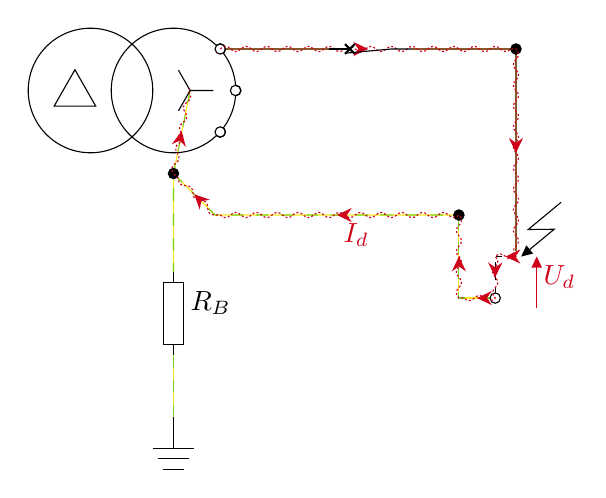
\begin{tikzpicture}[x=0.75pt,y=0.75pt,yscale=-1,xscale=1]
%uncomment if require: \path (0,251); %set diagram left start at 0, and has height of 251

%Straight Lines [id:da9415376086031365] 
\draw [color={rgb, 255:red, 0; green, 0; blue, 0 }  ,draw opacity=1 ] [dash pattern={on 2.25pt off 2.25pt}]  (242.5,132.5) -- (242.5,115) -- (252.5,115) ;
%Straight Lines [id:da5104591094158853] 
\draw [color={rgb, 255:red, 248; green, 231; blue, 28 }  ,draw opacity=1 ]   (87.5,75) -- (107.5,95) -- (225,95) ;
%Straight Lines [id:da1966201814177917] 
\draw [color={rgb, 255:red, 126; green, 211; blue, 33 }  ,draw opacity=1 ] [dash pattern={on 4.5pt off 4.5pt}]  (87.5,75) -- (107.5,95) -- (225,95) ;
%Straight Lines [id:da3955266461919331] 
\draw [color={rgb, 255:red, 248; green, 231; blue, 28 }  ,draw opacity=1 ]   (87.5,162.5) -- (87.5,192.5) ;
%Straight Lines [id:da18836033833143995] 
\draw [color={rgb, 255:red, 248; green, 231; blue, 28 }  ,draw opacity=1 ]   (240,135) -- (225,135) -- (225,95) ;
%Straight Lines [id:da17249205616306007] 
\draw [color={rgb, 255:red, 139; green, 87; blue, 42 }  ,draw opacity=1 ]   (112.5,15) -- (162.5,15) ;
%Straight Lines [id:da11309897556582038] 
\draw [color={rgb, 255:red, 248; green, 231; blue, 28 }  ,draw opacity=1 ]   (95.5,35) -- (87.5,75) -- (87.5,122.5) ;
%Straight Lines [id:da4238452834369957] 
\draw [color={rgb, 255:red, 126; green, 211; blue, 33 }  ,draw opacity=1 ] [dash pattern={on 4.5pt off 4.5pt}]  (95.5,35) -- (87.5,75) -- (87.5,122.5) ;
%Straight Lines [id:da07337279365918903] 
\draw [color={rgb, 255:red, 139; green, 87; blue, 42 }  ,draw opacity=1 ]   (202.5,15) -- (252.5,15) ;
%Shape: Path Data [id:dp3633653751506416] 
\draw   (112.5,55) .. controls (112.5,56.38) and (111.38,57.5) .. (110,57.5) .. controls (109.29,57.5) and (108.65,57.2) .. (108.19,56.72) .. controls (102.81,61.85) and (95.52,65) .. (87.5,65) .. controls (70.93,65) and (57.5,51.57) .. (57.5,35) .. controls (57.5,18.43) and (70.93,5) .. (87.5,5) .. controls (95.52,5) and (102.81,8.15) .. (108.19,13.28) .. controls (108.65,12.8) and (109.29,12.5) .. (110,12.5) .. controls (111.38,12.5) and (112.5,13.62) .. (112.5,15) .. controls (112.5,15.82) and (112.11,16.54) .. (111.5,17) .. controls (114.8,21.39) and (116.92,26.71) .. (117.4,32.5) .. controls (117.43,32.5) and (117.47,32.5) .. (117.5,32.5) .. controls (118.88,32.5) and (120,33.62) .. (120,35) .. controls (120,36.38) and (118.88,37.5) .. (117.5,37.5) .. controls (117.47,37.5) and (117.43,37.5) .. (117.4,37.5) .. controls (116.92,43.29) and (114.8,48.61) .. (111.5,53) .. controls (112.11,53.46) and (112.5,54.18) .. (112.5,55) -- cycle ;
%Shape: Circle [id:dp8103241388904666] 
\draw   (17.5,35) .. controls (17.5,18.43) and (30.93,5) .. (47.5,5) .. controls (64.07,5) and (77.5,18.43) .. (77.5,35) .. controls (77.5,51.57) and (64.07,65) .. (47.5,65) .. controls (30.93,65) and (17.5,51.57) .. (17.5,35) -- cycle ;
%Shape: Triangle [id:dp1236855376591316] 
\draw   (40,25) -- (30,42.5) -- (50,42.5) -- cycle ;
%Shape: Star [id:dp7604780706337534] 
\draw   (106.75,35) -- (95.5,35) -- (89.88,44.81) -- (95.5,35) -- (89.88,25.19) -- (95.5,35) -- cycle ;
%Shape: Circle [id:dp9987526738268633] 
\draw   (107.5,15) .. controls (107.5,13.62) and (108.62,12.5) .. (110,12.5) .. controls (111.38,12.5) and (112.5,13.62) .. (112.5,15) .. controls (112.5,16.38) and (111.38,17.5) .. (110,17.5) .. controls (108.62,17.5) and (107.5,16.38) .. (107.5,15) -- cycle ;
%Shape: Circle [id:dp06603296247595714] 
\draw   (114.9,35) .. controls (114.9,33.62) and (116.02,32.5) .. (117.4,32.5) .. controls (118.78,32.5) and (119.9,33.62) .. (119.9,35) .. controls (119.9,36.38) and (118.78,37.5) .. (117.4,37.5) .. controls (116.02,37.5) and (114.9,36.38) .. (114.9,35) -- cycle ;
%Shape: Circle [id:dp9864995024391362] 
\draw   (107.5,55) .. controls (107.5,53.62) and (108.62,52.5) .. (110,52.5) .. controls (111.38,52.5) and (112.5,53.62) .. (112.5,55) .. controls (112.5,56.38) and (111.38,57.5) .. (110,57.5) .. controls (108.62,57.5) and (107.5,56.38) .. (107.5,55) -- cycle ;

%Straight Lines [id:da23296631733343887] 
\draw [color={rgb, 255:red, 139; green, 87; blue, 42 }  ,draw opacity=1 ]   (252.5,112.5) -- (252.5,17.5) ;
%Straight Lines [id:da04537703273022686] 
\draw [color={rgb, 255:red, 126; green, 211; blue, 33 }  ,draw opacity=1 ] [dash pattern={on 4.5pt off 4.5pt}]  (240,135) -- (225,135) -- (225,95) ;
%Straight Lines [id:da014129266039552002] 
\draw    (87.5,192.5) -- (87.5,207.5) ;
%Straight Lines [id:da0064749529617041945] 
\draw    (77.5,207.5) -- (97.5,207.5) ;
%Straight Lines [id:da15495544426671526] 
\draw    (80,212.5) -- (95,212.5) ;
%Straight Lines [id:da9920646299152576] 
\draw    (82.5,217.5) -- (92.5,217.5) ;

%Straight Lines [id:da3741789060346865] 
\draw [color={rgb, 255:red, 126; green, 211; blue, 33 }  ,draw opacity=1 ] [dash pattern={on 4.5pt off 4.5pt}]  (87.5,162.5) -- (87.5,192.5) ;
%Straight Lines [id:da7734223518041439] 
\draw    (87.5,157.5) -- (87.5,162.5) ;
%Shape: Rectangle [id:dp997793865821069] 
\draw   (92.5,127.5) -- (92.5,157.5) -- (82.5,157.5) -- (82.5,127.5) -- cycle ;
%Straight Lines [id:da3149495431277475] 
\draw    (87.5,122.5) -- (87.5,127.5) ;

%Shape: Circle [id:dp16804091145958433] 
\draw  [fill={rgb, 255:red, 0; green, 0; blue, 0 }  ,fill opacity=1 ] (250,15) .. controls (250,13.62) and (251.12,12.5) .. (252.5,12.5) .. controls (253.88,12.5) and (255,13.62) .. (255,15) .. controls (255,16.38) and (253.88,17.5) .. (252.5,17.5) .. controls (251.12,17.5) and (250,16.38) .. (250,15) -- cycle ;
%Shape: Circle [id:dp448433802683451] 
\draw  [fill={rgb, 255:red, 255; green, 255; blue, 255 }  ,fill opacity=1 ] (240,135) .. controls (240,133.62) and (241.12,132.5) .. (242.5,132.5) .. controls (243.88,132.5) and (245,133.62) .. (245,135) .. controls (245,136.38) and (243.88,137.5) .. (242.5,137.5) .. controls (241.12,137.5) and (240,136.38) .. (240,135) -- cycle ;
%Shape: Circle [id:dp727181862391113] 
\draw  [fill={rgb, 255:red, 0; green, 0; blue, 0 }  ,fill opacity=1 ] (85,75) .. controls (85,73.62) and (86.12,72.5) .. (87.5,72.5) .. controls (88.88,72.5) and (90,73.62) .. (90,75) .. controls (90,76.38) and (88.88,77.5) .. (87.5,77.5) .. controls (86.12,77.5) and (85,76.38) .. (85,75) -- cycle ;
%Shape: Circle [id:dp14350658403367889] 
\draw  [fill={rgb, 255:red, 0; green, 0; blue, 0 }  ,fill opacity=1 ] (222.5,95) .. controls (222.5,93.62) and (223.62,92.5) .. (225,92.5) .. controls (226.38,92.5) and (227.5,93.62) .. (227.5,95) .. controls (227.5,96.38) and (226.38,97.5) .. (225,97.5) .. controls (223.62,97.5) and (222.5,96.38) .. (222.5,95) -- cycle ;
%Straight Lines [id:da09996473378362858] 
\draw [color={rgb, 255:red, 208; green, 2; blue, 27 }  ,draw opacity=1 ] [dash pattern={on 0.75pt off 0.75pt}]  (110,15) .. controls (111.67,13.33) and (113.33,13.33) .. (115,15) .. controls (116.67,16.67) and (118.33,16.67) .. (120,15) .. controls (121.67,13.33) and (123.33,13.33) .. (125,15) .. controls (126.67,16.67) and (128.33,16.67) .. (130,15) .. controls (131.67,13.33) and (133.33,13.33) .. (135,15) .. controls (136.67,16.67) and (138.33,16.67) .. (140,15) .. controls (141.67,13.33) and (143.33,13.33) .. (145,15) .. controls (146.67,16.67) and (148.33,16.67) .. (150,15) .. controls (151.67,13.33) and (153.33,13.33) .. (155,15) .. controls (156.67,16.67) and (158.33,16.67) .. (160,15) .. controls (161.67,13.33) and (163.33,13.33) .. (165,15) .. controls (166.67,16.67) and (168.33,16.67) .. (170,15) .. controls (171.67,13.33) and (173.33,13.33) .. (175,15) .. controls (176.67,16.67) and (178.33,16.67) .. (180,15) .. controls (181.67,13.33) and (183.33,13.33) .. (185,15) .. controls (186.67,16.67) and (188.33,16.67) .. (190,15) .. controls (191.67,13.33) and (193.33,13.33) .. (195,15) .. controls (196.67,16.67) and (198.33,16.67) .. (200,15) .. controls (201.67,13.33) and (203.33,13.33) .. (205,15) .. controls (206.67,16.67) and (208.33,16.67) .. (210,15) .. controls (211.67,13.33) and (213.33,13.33) .. (215,15) .. controls (216.67,16.67) and (218.33,16.67) .. (220,15) .. controls (221.67,13.33) and (223.33,13.33) .. (225,15) .. controls (226.67,16.67) and (228.33,16.67) .. (230,15) .. controls (231.67,13.33) and (233.33,13.33) .. (235,15) .. controls (236.67,16.67) and (238.33,16.67) .. (240,15) .. controls (241.67,13.33) and (243.33,13.33) .. (245,15) .. controls (246.67,16.67) and (248.33,16.67) .. (250,15) -- (252.5,15) -- (252.5,15) .. controls (254.17,16.67) and (254.17,18.33) .. (252.5,20) .. controls (250.83,21.67) and (250.83,23.33) .. (252.5,25) .. controls (254.17,26.67) and (254.17,28.33) .. (252.5,30) .. controls (250.83,31.67) and (250.83,33.33) .. (252.5,35) .. controls (254.17,36.67) and (254.17,38.33) .. (252.5,40) .. controls (250.83,41.67) and (250.83,43.33) .. (252.5,45) .. controls (254.17,46.67) and (254.17,48.33) .. (252.5,50) .. controls (250.83,51.67) and (250.83,53.33) .. (252.5,55) .. controls (254.17,56.67) and (254.17,58.33) .. (252.5,60) .. controls (250.83,61.67) and (250.83,63.33) .. (252.5,65) .. controls (254.17,66.67) and (254.17,68.33) .. (252.5,70) .. controls (250.83,71.67) and (250.83,73.33) .. (252.5,75) .. controls (254.17,76.67) and (254.17,78.33) .. (252.5,80) .. controls (250.83,81.67) and (250.83,83.33) .. (252.5,85) .. controls (254.17,86.67) and (254.17,88.33) .. (252.5,90) .. controls (250.83,91.67) and (250.83,93.33) .. (252.5,95) .. controls (254.17,96.67) and (254.17,98.33) .. (252.5,100) .. controls (250.83,101.67) and (250.83,103.33) .. (252.5,105) .. controls (254.17,106.67) and (254.17,108.33) .. (252.5,110) .. controls (250.83,111.67) and (250.83,113.33) .. (252.5,115) -- (252.5,115) .. controls (250.83,116.67) and (249.17,116.67) .. (247.5,115) .. controls (245.83,113.33) and (244.17,113.33) .. (242.5,115) -- (242.5,115) .. controls (244.17,116.67) and (244.17,118.33) .. (242.5,120) .. controls (240.83,121.67) and (240.83,123.33) .. (242.5,125) .. controls (244.17,126.67) and (244.17,128.33) .. (242.5,130) .. controls (240.83,131.67) and (240.83,133.33) .. (242.5,135) -- (242.5,135) -- (242.5,135) .. controls (240.83,136.67) and (239.17,136.67) .. (237.5,135) .. controls (235.83,133.33) and (234.17,133.33) .. (232.5,135) .. controls (230.83,136.67) and (229.17,136.67) .. (227.5,135) -- (225,135) -- (225,135) .. controls (223.33,133.33) and (223.33,131.67) .. (225,130) .. controls (226.67,128.33) and (226.67,126.67) .. (225,125) .. controls (223.33,123.33) and (223.33,121.67) .. (225,120) .. controls (226.67,118.33) and (226.67,116.67) .. (225,115) .. controls (223.33,113.33) and (223.33,111.67) .. (225,110) .. controls (226.67,108.33) and (226.67,106.67) .. (225,105) .. controls (223.33,103.33) and (223.33,101.67) .. (225,100) .. controls (226.67,98.33) and (226.67,96.67) .. (225,95) -- (225,95) -- (225,95) .. controls (223.33,96.67) and (221.67,96.67) .. (220,95) .. controls (218.33,93.33) and (216.67,93.33) .. (215,95) .. controls (213.33,96.67) and (211.67,96.67) .. (210,95) .. controls (208.33,93.33) and (206.67,93.33) .. (205,95) .. controls (203.33,96.67) and (201.67,96.67) .. (200,95) .. controls (198.33,93.33) and (196.67,93.33) .. (195,95) .. controls (193.33,96.67) and (191.67,96.67) .. (190,95) .. controls (188.33,93.33) and (186.67,93.33) .. (185,95) .. controls (183.33,96.67) and (181.67,96.67) .. (180,95) .. controls (178.33,93.33) and (176.67,93.33) .. (175,95) .. controls (173.33,96.67) and (171.67,96.67) .. (170,95) .. controls (168.33,93.33) and (166.67,93.33) .. (165,95) .. controls (163.33,96.67) and (161.67,96.67) .. (160,95) .. controls (158.33,93.33) and (156.67,93.33) .. (155,95) .. controls (153.33,96.67) and (151.67,96.67) .. (150,95) .. controls (148.33,93.33) and (146.67,93.33) .. (145,95) .. controls (143.33,96.67) and (141.67,96.67) .. (140,95) .. controls (138.33,93.33) and (136.67,93.33) .. (135,95) .. controls (133.33,96.67) and (131.67,96.67) .. (130,95) .. controls (128.33,93.33) and (126.67,93.33) .. (125,95) .. controls (123.33,96.67) and (121.67,96.67) .. (120,95) .. controls (118.33,93.33) and (116.67,93.33) .. (115,95) .. controls (113.33,96.67) and (111.67,96.67) .. (110,95) -- (107.5,95) -- (107.5,95) .. controls (105.14,95) and (103.96,93.82) .. (103.96,91.46) .. controls (103.96,89.11) and (102.78,87.93) .. (100.43,87.93) .. controls (98.07,87.93) and (96.89,86.75) .. (96.89,84.39) .. controls (96.89,82.04) and (95.71,80.86) .. (93.36,80.86) .. controls (91,80.86) and (89.82,79.68) .. (89.82,77.32) -- (87.5,75) -- (87.5,75) .. controls (86.17,73.05) and (86.48,71.42) .. (88.43,70.09) .. controls (90.38,68.76) and (90.69,67.12) .. (89.36,65.17) .. controls (88.03,63.22) and (88.34,61.59) .. (90.29,60.26) .. controls (92.24,58.93) and (92.54,57.3) .. (91.21,55.35) .. controls (89.88,53.4) and (90.19,51.77) .. (92.14,50.44) .. controls (94.09,49.11) and (94.4,47.47) .. (93.07,45.52) .. controls (91.74,43.57) and (92.05,41.94) .. (94,40.61) .. controls (95.95,39.28) and (96.26,37.65) .. (94.93,35.7) -- (95.25,34) -- (95.25,34) ;
\draw [shift={(181.25,15)}, rotate = 180] [fill={rgb, 255:red, 208; green, 2; blue, 27 }  ,fill opacity=1 ][line width=0.08]  [draw opacity=0] (7.14,-3.43) -- (0,0) -- (7.14,3.43) -- (4.74,0) -- cycle    ;
\draw [shift={(252.5,65)}, rotate = 270] [fill={rgb, 255:red, 208; green, 2; blue, 27 }  ,fill opacity=1 ][line width=0.08]  [draw opacity=0] (7.14,-3.43) -- (0,0) -- (7.14,3.43) -- (4.74,0) -- cycle    ;
\draw [shift={(247.5,115)}, rotate = 360] [fill={rgb, 255:red, 208; green, 2; blue, 27 }  ,fill opacity=1 ][line width=0.08]  [draw opacity=0] (7.14,-3.43) -- (0,0) -- (7.14,3.43) -- (4.74,0) -- cycle    ;
\draw [shift={(242.5,125)}, rotate = 270] [fill={rgb, 255:red, 208; green, 2; blue, 27 }  ,fill opacity=1 ][line width=0.08]  [draw opacity=0] (7.14,-3.43) -- (0,0) -- (7.14,3.43) -- (4.74,0) -- cycle    ;
\draw [shift={(233.75,135)}, rotate = 360] [fill={rgb, 255:red, 208; green, 2; blue, 27 }  ,fill opacity=1 ][line width=0.08]  [draw opacity=0] (7.14,-3.43) -- (0,0) -- (7.14,3.43) -- (4.74,0) -- cycle    ;
\draw [shift={(225,115)}, rotate = 450] [fill={rgb, 255:red, 208; green, 2; blue, 27 }  ,fill opacity=1 ][line width=0.08]  [draw opacity=0] (7.14,-3.43) -- (0,0) -- (7.14,3.43) -- (4.74,0) -- cycle    ;
\draw [shift={(166.25,95)}, rotate = 360] [fill={rgb, 255:red, 208; green, 2; blue, 27 }  ,fill opacity=1 ][line width=0.08]  [draw opacity=0] (7.14,-3.43) -- (0,0) -- (7.14,3.43) -- (4.74,0) -- cycle    ;
\draw [shift={(97.5,85)}, rotate = 405] [fill={rgb, 255:red, 208; green, 2; blue, 27 }  ,fill opacity=1 ][line width=0.08]  [draw opacity=0] (7.14,-3.43) -- (0,0) -- (7.14,3.43) -- (4.74,0) -- cycle    ;
\draw [shift={(91.38,54.5)}, rotate = 460.7] [fill={rgb, 255:red, 208; green, 2; blue, 27 }  ,fill opacity=1 ][line width=0.08]  [draw opacity=0] (7.14,-3.43) -- (0,0) -- (7.14,3.43) -- (4.74,0) -- cycle    ;
%Shape: Boxed Line [id:dp3673372749832414] 
\draw    (274.27,88.83) -- (258.39,101.97) -- (270.89,101.86) -- (257.31,113.09) ;
\draw [shift={(255,115)}, rotate = 320.40999999999997] [fill={rgb, 255:red, 0; green, 0; blue, 0 }  ][line width=0.08]  [draw opacity=0] (5.36,-2.57) -- (0,0) -- (5.36,2.57) -- cycle    ;
%Straight Lines [id:da5575509867036751] 
\draw    (170.5,17) -- (192.5,15) -- (202.5,15) ;
%Straight Lines [id:da508912305096757] 
\draw    (172.5,15) -- (162.5,15) ;
\draw [shift={(172.5,15)}, rotate = 225] [color={rgb, 255:red, 0; green, 0; blue, 0 }  ][line width=0.75]    (-3.35,0) -- (3.35,0)(0,3.35) -- (0,-3.35)   ;

%Straight Lines [id:da16958097231268054] 
\draw [color={rgb, 255:red, 208; green, 2; blue, 27 }  ,draw opacity=1 ]   (262.5,118) -- (262.5,140) ;
\draw [shift={(262.5,115)}, rotate = 90] [fill={rgb, 255:red, 208; green, 2; blue, 27 }  ,fill opacity=1 ][line width=0.08]  [draw opacity=0] (5.36,-2.57) -- (0,0) -- (5.36,2.57) -- cycle    ;


% Text Node
\draw (94.5,130.5) node [anchor=north west][inner sep=0.75pt]   [align=left] {$R_B$};
% Text Node
\draw (168.25,98) node [anchor=north west][inner sep=0.75pt]  [color={rgb, 255:red, 208; green, 2; blue, 27 }  ,opacity=1 ] [align=left] {$I_d$};
% Text Node
\draw (264.5,118) node [anchor=north west][inner sep=0.75pt]  [color={rgb, 255:red, 208; green, 2; blue, 27 }  ,opacity=1 ] [align=left] {$U_d$};


\end{tikzpicture}

\end{figure}

%\end{document}



Pour calculer le courant de défaut $I_d$, il existe trois méthode, mais ne sera détaillé dans ce chapitre que la première (plus de précisions sur les deux autres méthode \superref{ann:schema_tn}) :
\begin{itemize}
\item Méthode conventionnelle\,;
\item Méthode des impédances\,;
\item Méthode de composition.
\end{itemize}

\section{Méthode de dimensionnement conventionnelle des protections et des sections de conducteurs\label{sec:schema_tn_methode_conventionnelle}}

Contrairement au SLT TT, il ne faut pas tenir compte de la \emph{résistance de défaut} $R_d$ qui prend en compte la nature du défaut d'isolement (franc ou non-franc) et la résistance de la carcasse métallique car il s'agit d'un court-circuit et elle sera donc très faible.\\
$I_d$ s'apparente donc à un courant de court-circuit et son calcul est basé sur l'hypothèse que la tension de défaut reste supérieur à 80\% ou plus de la tension nominale simple. Cette valeur est issue d'une estimation de la chute de tension due à l'ensemble des impédances en amont de la protection du circuit en défaut. Elle est utilisée, avec l'impédance de la boucle de circuit, pour calculer ce courant de court-circuit.\\ 

Ce facteur est calculé par l'estimation de la chute de tension due à l'ensemble des impédances en amont de cette origine. Dans une majorité des types de pose, les réactances inductive interne et entres les conducteurs sont négligées, ce qui revient à ne considérer que les résistances des conducteurs dans les calculs d'intensité de court-circuit. Cette approximation est considérée comme valable pour les sections de câble jusqu'à \SI{120}{\square\milli\meter}. Au-dessus de cette section, la résistance $R$ des conducteurs est augmentée selon le tableau ci-dessous :

\begin{table}[H]
\caption{Section des conducteurs (schéma TN / méthode conventionnelle)}
\begin{tabular}{O k@{${\enspace{}}+{\enspace{}}$}i}
\toprule
\multicolumn{2}{c}{\thead{Section des conducteurs}} & \multicolumn{2}{c}{\thead{Ajustement de la résistance en \si{\ohm}}} \\
\midrule
S & \SI{150}{\square\milli\meter} & R & 15\% \\
S & \SI{185}{\square\milli\meter} & R & 20\% \\
S & \SI{240}{\square\milli\meter} & R & 25\% \\
\bottomrule
\end{tabular}
\end{table}

\begin{formule}[Courant de défaut $I_d$ en schéma TN selon la méthode conventionnelle\label{form:courant_defaut_tn_conventionnel}]
\begin{align*}
		I_d &= \frac{0,8 \times U_{0}}{R_{PE}+R_{ph}} \\
		I_d &= \frac{0,8 \times U_{0}}{Z_{c}}
\end{align*}
\end{formule}

\begin{textvariables}
U_{0}						& tension							& volt			& \volt					& 	Tension nominale simple \\
0,8							& facteur							& 					& 	/						& 	facteur d'approximation de la tension de défaut $U_d$ \\
R_{PE}						& résistance						& ohm			& \ohm					& 	Résistance du conducteur de phase traversé par un courant de défaut $I_d$	\\
R_{ph}						& résistance						& ohm			& \ohm					& 	Résistance du conducteur PE traversé par un courant de défaut $I_d$ \\
Z_{c}						& impédance						& ohm			& \ohm					& Impédance de boucle du circuit en défaut (selon la méthode conventionnelle)\\
\end{textvariables}

Le courant de défaut $I_d$ fera alors apparaître une \emph{tension de défaut} $U_d$ entre la masse métallique et la terre :

\begin{formule}[Tension de défaut $U_d$ en schéma TN selon la méthode conventionnelle] 
\begin{align*}
		U_d &= R_{PE} \times I_{d}
\end{align*}
\end{formule}

\begin{textvariables}
R_{PE}						& résistance						& ohm			& \ohm					& 	Résistance du conducteur PE traversé par un courant de défaut $I_d$	\\
I_{d}							& intensité							& ampère		& \ampere				& 	Courant de défaut d'isolement \\
\end{textvariables}

La tension de défaut $U_d$ dans le cas d'un défaut d'isolement en régime TN est \emph{élevée} et donc \emph{dangereuse} si elle est supportée trop longtemps. La norme NF C15-100 a défini des temps de coupure maximum à respecter :

\input{tab_schema_tn_temps_coupure}

\begin{formule}[Seuil de réglage du disjoncteur $I_m$ en schéma TN]
\begin{align*}
		I_{m} &> I_{d}
\end{align*}
\end{formule}

\begin{textvariables}
I_{m}						& intensité							& ampère			& \ampere					& 	Intensité de seuil de déclenchement de la protection magnétique du disjoncteur \\
\end{textvariables}

On peut calculer la longueur maximale d'un circuit d'une installation en schéma TN par la formule suivante 

\begin{formule}[Longueur maximale d'un circuit $L_{max}$\label{form:schema_tn_longueur_max_circuit}]
\begin{align*}
		L_{max} &= \frac{0,8 \times U_{0} \times S_{ph}}{\rho \times (1+m) \times I_m}\\
		m &= \frac{S_{ph}}{S_{PE}}
\end{align*}
\end{formule}
\begin{textvariables}
I_{m}						& intensité							& ampère			& \ampere							& 	Intensité de seuil de déclenchement de la protection magnétique du disjoncteur \\
U_{0}						& tension							& volt				& \volt								& 	Tension nominale simple \\
S_{ph}						& section							& millimètre\up{2}		& \si{\square\milli\meter}	& 	Section du conducteur de phase traversé par un courant de défaut $I_d$ \\
S_{PE}						& section							& millimètre\up{2}		& \si{\square\milli\meter}	& 	Section du conducteur PE traversé par un courant de défaut $I_d$ \\
\rho							& résistivité						& 		& \si{\ohm\square\milli\meter\per\meter}	& 	Résistivité du conducteur (selon la température et le matériau choisi) :
\begin{tabdescription}
\item[aluminium :] \SI{37.6 \times 10^{-3}}{\ohm\square\milli\meter\per\meter}
\item[cuivre :] \SI{22.5 \times 10^{-3}}{\ohm\square\milli\meter\per\meter}
\end{tabdescription}\\
m								& facteur		& 			& /										& Facteur de correction à appliquer aux valeurs données dans les abaques de détermination des longueurs selon la section et l'intensité de déclenchement (\superref{subsubsec:facteur_correction_m}) 	 \\
\end{textvariables}

Pour vérifier rapidement un dimensionnement, les constructeurs de protections ont établis des abaques permettant de déterminer rapidement les longueurs maximale des conducteurs selon l'intensité, la section des conducteurs ou en encore les réglages du seuil de courant de déclenchement du disjoncteur ou encore le type de disjoncteurs. Ces abaques sont issus des norme IEC 60947-2\supercite{IEC:60947-2-2016} et IEC 60898\supercite{IEC:60898-2015}, qui concernent respectivement les disjoncteurs industriels et domestiques. Ils sont détaillés dans l'annexe \superref{ann:schema_tn}.

\begin{exemple}[Calcul du courant de défaut $I_d$ en schéma TN]
Si on considère que les conducteurs sont en cuivre, que $U_{0}=\SI{230}{\volt}$, que $L_{ph}=\SI{50}{\meter}$ et est équivalent à $L_{PE}$, que $S_{ph}=\SI{35}{\square\milli\meter}$ et est équivalent à  $S_{PE}$, on peut déduire que le courant de défaut $I_d$ vaut :
\begin{align*}
		Z_{c}	&= 2 \times \rho \times \frac{L}{S}  								& 			I_d		&= \frac{U_0 \times 0,8}{Z_c} \\
					&= 2 \times 22.5 \times 10^{-3} \times \frac{50}{35} 	&						&= \frac{230 \times 0,8}{64,3 \times 10^{-3}} \\
					&= \SI{64,3}{\milli\ohm}						 						& 						&= \SI{2816}{\ampere}
\end{align*}
\end{exemple}

\begin{exemple}[Calcul de la longueur maximale des conducteurs $L_{max}$ en schéma TN]
Si on considère que les conducteurs sont en cuivre, que $U_{0}=\SI{230}{\volt}$, que $L{ph}=\SI{50}{\meter}$ et est équivalent à $L{PE}$, que $S_{ph}=\SI{35}{\square\milli\meter}$ et est équivalent à  $S_{PE}$, on peut déduire que le courant de défaut $I_d$ vaut :
\begin{align*}
		Z_{c}	&= 2 \times \rho \times \frac{L}{S}  								& 			I_d		&= \frac{U_0 \times 0,8}{Z_c} \\
					&= 2 \times 22.5 \times 10^{-3} \times \frac{50}{35} 			&				&= \frac{230 \times 0,8}{64,3e \times 10^{-3}} \\
					&= \SI{64,3}{\milli\ohm}						 						& 						&= \SI{2816}{\ampere}
\end{align*}

Il convient de croiser cette valeur de $I_d$ avec les valeurs du seuil de déclenchement du disjoncteur Instantané et Court-retard et leurs temps de coupures respectifs (voir \superref{tab:schema_tn_temps_coupure}) pour valider le dimensionnement et le choix de la protection.

\end{exemple}

\section{Protection avec des DDR en schéma TN}

La protection des circuits à l'aide de DDR en schéma TN est formellement interdite en schéma TN-C car le conducteur PE ne peut pas être sectionné. En schéma TN-C-S, son utilisation implique forcément que les conducteurs PE et N soient séparés en amont du DDR.\\

Les DDR en schéma TN-S sont requis lorsque :
\begin{itemize}
\item l'impédance de la boucle de défaut $Z_c$ n'est pas précisément calculable\,;
\item le courant de défaut est trop faible pour que la protection détecte le défaut comme s'apparentant à un court-circuit dans le temps de déconnexion requis.
\end{itemize}

Un DDR se déclenchant avec un courant de déclenchement de l'ordre que quelques ampères maximum, il convient bien à un circuit terminal d'une installation BT conséquente en schéma TN.





%\end{document}

	%--------------------------------------
%ELECTROTECHNIQUE - SCHEMA DE LIAISON A LA TERRE
%--------------------------------------

%utiliser les environnement \begin{comment} \end{comment} pour mettre en commentaire le préambule une fois la programmation appelée dans le document maître (!ne pas oublier de mettre en commentaire \end{document}!)

\begin{comment}

\documentclass[a4paper, 11pt, twoside, fleqn]{memoir}

\usepackage{AOCDTF}

\marqueurchapitre
\decoupagechapitre{1} %juste pour éviter les erreurs lors de la compilation des sous-programmations (passera en commentaire)

%--------------------------------------
%corps du document
%--------------------------------------

\begin{document} %corps du document
	\openleft %début de chapitre à gauche

\end{comment}

\chapter{Schéma Impédant-Terre\label{chap:schema_it}}
\ChapFrame

\section{Caractéristiques générales}

\begin{definition}[Schéma IT]
Schéma de liaison à la terre dans lequel le prise de terre du neutre du transformateur et la prise de terre des masses métalliques sont raccordées à la terre selon quatre variantes différentes :
\begin{figure}[H]
\begin{tabularx}{\linewidth}{XXXX}
\toprule
\multicolumn{2}{c}{\thead{Neutre transformateur HT/BT}} & \multicolumn{2}{c}{\thead{Masses conductrices}} \\
\cmidrule(lr){1-2} 	\cmidrule(lr){3-4}
\thead{Isolé ($Z_{res}$)}	& \thead{Impédant ($Z_{N}$)}	& \thead{Interconnectées}	& \thead{Individuelles} \\
\midrule
Neutre du transformateur pas raccordé du tout. Terme \og isolé \fg{} à nuancer car l'installation électrique en aval du transformateur HT/BT ne sera jamais complètement isolée par rapport à la terre. Il subsistera toujours un courant de défaut $I_d$ plus ou moins minime due à une impédance de fuite $Z_{res}$ présente dans tous les réseaux électriques (voir \superref{sec:isolation_installation_schema_it}).
& 
Neutre du transformateur raccordé à la prise de terre par une \emph{impédance de limitation} dont la valeur dépend de la fréquence de la tension :
\begin{compactitemize}
\item$F=\SI{50}{\hertz}$ : \SI{1500}{\ohm}\,;
\item$F=\SI{2,5}{\hertz}$ : \SI{2,5}{\ohm}.
\end{compactitemize}
Cette impédance fixe donc une différence de potentiel définie entre le neutre et la terre, elle est installée lorsque le réseau électrique est court et que l'impédance de fuite $Z_{res}$ est élevée.
&
Masses \emph{interconnectées} au moyen d'un conducteur PE et raccordées à la terre au niveau du transformateur HT/BT. Raccordement similaire au schéma TN, à la différence que le neutre du transformateur n'est pas raccordé au conducteur PE et à la terre.
&
Masses mise à la terre \emph{individuellement} ou par groupe à des prises de terre propres. Type de raccordement similaire au schéma TT avec installation de DDR en tête de chaque circuit.
\end{tabularx}
\end{figure}
\end{definition}

Il s'agit d'un SLT un peu plus atypique ayant pour but d'assurer une \emph{continuité de service} à l'installation électrique malgré un \emph{premier défaut d'isolement} tout en assurant la protection des personnes contre les contacts indirects. Selon les quatre variantes de raccordement, le premier défaut entrainera un fonctionnement identique des protections mais à l'apparition d'un deuxième défaut entrainera un fonctionnement des protection différent.\\

Dans la pratique, le schéma IT présente les caractéristiques suivantes :
\begin{itemize}
\item continuité de service assurée après un premier défaut d'isolement\,;
\item contrôle permanent de l'isolement de l'installation par rapport à la terre avec signalisation de toute dépassement du seuil d'isolement défini à l'aide d'un Contrôleur Permanent d'Isolement (CPI)\,;
\item protection du neutre assurée\,;
\item raccordement possible d'un limiteur de tension (éclateur) entre la terre et le point neutre du transformateur HT/BT\,;
\item présence continue d'une équipe pour assurer rapidement la recherche du premier défaut d'isolement aussitôt signalé, facilitée avec du matériel de localisation automatique\,;
\item coupure automatique de l'installation dès l'apparition d'un second défaut d'isolement sur un conducteur actif différent de celui ou le premier défaut d'isolement est apparu.
\end{itemize}

Le courant de défaut du premier défaut d'isolement va dépendre de l'impédance de limitation du neutre et de l'état d'isolement de l'installation électrique. Pour toutefois protéger les personnes, il doit être suffisamment bas pour satisfaire la règle $I_{d} \times R_{A} \pm \SI{50}{\volt}$, de sorte à ce que la tension de défaut $U_d$ ne présente aucun danger.

\section{Isolation de l'installation électrique en schéma IT\label{sec:isolation_installation_schema_it}}

Dans le cas d'un schéma IT ou le neutre est isolé, l'isolement de l'installation de l'installation électrique n'est pas infini par rapport à la terre car les isolants ne présentent jamais une résistance infinie. Une résistance de fuite du de l'installation électrique apparaitra toujours et dépendra de plusieurs facteurs :
\begin{itemize}
\item nature des isolants (PVC, air\ldots)\,;
\item âge de l'installation
\item degré d'humidité\,;
\item longueur de l'installation.
\end{itemize}
Pour une installation neuve, on considère que la résistance de fuite est estimée à \SI{3,3}{\mega\ohm} pour \SI{1}{\kilo\meter} de réseau électrique.
\begin{formule}[Résistance de fuite du réseaux $R_{res}$ d'une installation neuve]
\begin{align*}
	R_{res} &= \frac{3,3}{n}
\end{align*} 
\end{formule}
\begin{textvariables}
R_{res}						& résistance					& méga-ohm			& \mega\ohm							& 	Résistance de fuite du réseaux électrique \\
n								& 									& 							& /										& 	Nombre de \si{\kilo\meter} de réseaux électrique \\
\end{textvariables}

%--------------------------------------
%ELECTROTECHNIQUE - SCHEMA DE LIAISON A LA TERRE
%--------------------------------------

%utiliser les environnement \begin{comment} \end{comment} pour mettre en commentaire le préambule une fois la programmation appelée dans le document maître (!ne pas oublier de mettre en commentaire \end{document}!)

\begin{comment}

\documentclass[a4paper, 11pt, twoside, fleqn]{memoir}

\usepackage{AOCDTF}

\marqueurchapitre
\decoupagechapitre{1} %juste pour éviter les erreurs lors de la compilation des sous-programmations (passera en commentaire)

%lien d'édition des figures Tikz sur le site mathcha.io (rajouter le lien d'une modification effectuée sur la figure tikz avec le nom du modificateur car il n'y a qu'un lien par compte)

%lien mathcha Bruno Douchy : https://www.mathcha.io/editor/Kxxn3cWBUm3T7ynYmWi4KY0P9H9d6v9qFLQyMEE

%--------------------------------------
%corps du document
%--------------------------------------

\begin{document} %corps du document
	\openleft %début de chapitre à gauche

\end{comment}


% Pattern Info
\begin{figure}[H]
\caption{Résistance de fuite $R_{res}$ d'un réseau électrique de plusieurs \si{\kilo\meter}}

% Pattern Info
 
\tikzset{
pattern size/.store in=\mcSize, 
pattern size = 5pt,
pattern thickness/.store in=\mcThickness, 
pattern thickness = 0.3pt,
pattern radius/.store in=\mcRadius, 
pattern radius = 1pt}
\makeatletter
\pgfutil@ifundefined{pgf@pattern@name@_sgw0g8yxt}{
\pgfdeclarepatternformonly[\mcThickness,\mcSize]{_sgw0g8yxt}
{\pgfqpoint{0pt}{0pt}}
{\pgfpoint{\mcSize+\mcThickness}{\mcSize+\mcThickness}}
{\pgfpoint{\mcSize}{\mcSize}}
{
\pgfsetcolor{\tikz@pattern@color}
\pgfsetlinewidth{\mcThickness}
\pgfpathmoveto{\pgfqpoint{0pt}{0pt}}
\pgfpathlineto{\pgfpoint{\mcSize+\mcThickness}{\mcSize+\mcThickness}}
\pgfusepath{stroke}
}}
\makeatother
\tikzset{every picture/.style={line width=0.75pt}} %set default line width to 0.75pt        

\begin{tikzpicture}[x=0.75pt,y=0.75pt,yscale=-1,xscale=1]
%uncomment if require: \path (0,327); %set diagram left start at 0, and has height of 327

%Straight Lines [id:da08009100326878149] 
\draw    (105,35) -- (210,35) ;
%Shape: Circle [id:dp3640107906362746] 
\draw   (2.5,35) .. controls (2.5,18.43) and (15.93,5) .. (32.5,5) .. controls (49.07,5) and (62.5,18.43) .. (62.5,35) .. controls (62.5,51.57) and (49.07,65) .. (32.5,65) .. controls (15.93,65) and (2.5,51.57) .. (2.5,35) -- cycle ;
%Straight Lines [id:da571377768464931] 
\draw    (30,232.5) -- (545,232.5) ;
%Straight Lines [id:da08045007432417306] 
\draw    (210,247.5) -- (210,262.5) ;
%Straight Lines [id:da4313577623259258] 
\draw    (200,262.5) -- (220,262.5) ;
%Straight Lines [id:da5912684771420953] 
\draw    (202.5,267.5) -- (217.5,267.5) ;
%Straight Lines [id:da13165123057200734] 
\draw    (205,272.5) -- (215,272.5) ;

%Straight Lines [id:da320941654963934] 
\draw    (210,217.5) -- (210,222.5) ;
%Shape: Rectangle [id:dp24059175551770873] 
\draw   (215,187.5) -- (215,217.5) -- (205,217.5) -- (205,187.5) -- cycle ;
%Straight Lines [id:da9352215304977288] 
\draw    (210,182.5) -- (210,187.5) ;

%Shape: Circle [id:dp5173960999636192] 
\draw   (45,35) .. controls (45,18.43) and (58.43,5) .. (75,5) .. controls (91.57,5) and (105,18.43) .. (105,35) .. controls (105,51.57) and (91.57,65) .. (75,65) .. controls (58.43,65) and (45,51.57) .. (45,35) -- cycle ;
%Straight Lines [id:da826385807465586] 
\draw    (140,45) -- (150,25) ;
\draw [shift={(150,25)}, rotate = 296.57] [color={rgb, 255:red, 0; green, 0; blue, 0 }  ][fill={rgb, 255:red, 0; green, 0; blue, 0 }  ][line width=0.75]      (0, 0) circle [x radius= 2.01, y radius= 2.01]   ;
%Straight Lines [id:da9637899679537502] 
\draw    (120,45) -- (130,25) ;
%Straight Lines [id:da6640472127950414] 
\draw    (115,45) -- (125,25) ;
%Straight Lines [id:da46557993038086076] 
\draw    (110,45) -- (120,25) ;

%Straight Lines [id:da33735776097392156] 
\draw    (210,222.5) -- (210,247.5) ;
%Straight Lines [id:da5122217943063542] 
\draw    (210,35) -- (210,182.5) ;
%Shape: Circle [id:dp05291492243843332] 
\draw  [fill={rgb, 255:red, 0; green, 0; blue, 0 }  ,fill opacity=1 ] (207.5,35) .. controls (207.5,33.62) and (208.62,32.5) .. (210,32.5) .. controls (211.38,32.5) and (212.5,33.62) .. (212.5,35) .. controls (212.5,36.38) and (211.38,37.5) .. (210,37.5) .. controls (208.62,37.5) and (207.5,36.38) .. (207.5,35) -- cycle ;
%Straight Lines [id:da6377337353392218] 
\draw    (212.5,35) -- (317.5,35) ;
%Straight Lines [id:da25115314727149973] 
\draw    (317.5,247.5) -- (317.5,262.5) ;
%Straight Lines [id:da901440360563758] 
\draw    (307.5,262.5) -- (327.5,262.5) ;
%Straight Lines [id:da7842646096579663] 
\draw    (310,267.5) -- (325,267.5) ;
%Straight Lines [id:da18808830899848483] 
\draw    (312.5,272.5) -- (322.5,272.5) ;

%Straight Lines [id:da49919296084643217] 
\draw    (317.5,217.5) -- (317.5,222.5) ;
%Shape: Rectangle [id:dp5156050966431545] 
\draw   (322.5,187.5) -- (322.5,217.5) -- (312.5,217.5) -- (312.5,187.5) -- cycle ;
%Straight Lines [id:da9531373030412352] 
\draw    (317.5,182.5) -- (317.5,187.5) ;

%Straight Lines [id:da8099985845539385] 
\draw    (247.5,45) -- (257.5,25) ;
\draw [shift={(257.5,25)}, rotate = 296.57] [color={rgb, 255:red, 0; green, 0; blue, 0 }  ][fill={rgb, 255:red, 0; green, 0; blue, 0 }  ][line width=0.75]      (0, 0) circle [x radius= 2.01, y radius= 2.01]   ;
%Straight Lines [id:da8087453766565224] 
\draw    (227.5,45) -- (237.5,25) ;
%Straight Lines [id:da3541011282357912] 
\draw    (222.5,45) -- (232.5,25) ;
%Straight Lines [id:da4838872480993197] 
\draw    (217.5,45) -- (227.5,25) ;

%Straight Lines [id:da6527379034333531] 
\draw    (317.5,222.5) -- (317.5,247.5) ;
%Straight Lines [id:da5530613085402983] 
\draw    (317.5,35) -- (317.5,182.5) ;
%Shape: Circle [id:dp25176527117973546] 
\draw  [fill={rgb, 255:red, 0; green, 0; blue, 0 }  ,fill opacity=1 ] (315,35) .. controls (315,33.62) and (316.12,32.5) .. (317.5,32.5) .. controls (318.88,32.5) and (320,33.62) .. (320,35) .. controls (320,36.38) and (318.88,37.5) .. (317.5,37.5) .. controls (316.12,37.5) and (315,36.38) .. (315,35) -- cycle ;
%Straight Lines [id:da18023630680839797] 
\draw    (320,35) -- (425,35) ;
%Straight Lines [id:da6476101136895756] 
\draw    (425,247.5) -- (425,262.5) ;
%Straight Lines [id:da4732182664219796] 
\draw    (415,262.5) -- (435,262.5) ;
%Straight Lines [id:da9789341071401707] 
\draw    (417.5,267.5) -- (432.5,267.5) ;
%Straight Lines [id:da9061441462289892] 
\draw    (420,272.5) -- (430,272.5) ;

%Straight Lines [id:da5168046359577328] 
\draw    (425,217.5) -- (425,222.5) ;
%Shape: Rectangle [id:dp6616267367458876] 
\draw   (430,187.5) -- (430,217.5) -- (420,217.5) -- (420,187.5) -- cycle ;
%Straight Lines [id:da5013364563135433] 
\draw    (425,182.5) -- (425,187.5) ;

%Straight Lines [id:da8467083023662558] 
\draw    (355,45) -- (365,25) ;
\draw [shift={(365,25)}, rotate = 296.57] [color={rgb, 255:red, 0; green, 0; blue, 0 }  ][fill={rgb, 255:red, 0; green, 0; blue, 0 }  ][line width=0.75]      (0, 0) circle [x radius= 2.01, y radius= 2.01]   ;
%Straight Lines [id:da8678289301466517] 
\draw    (335,45) -- (345,25) ;
%Straight Lines [id:da902125655347565] 
\draw    (330,45) -- (340,25) ;
%Straight Lines [id:da33092289865462876] 
\draw    (325,45) -- (335,25) ;

%Straight Lines [id:da6870106618089796] 
\draw    (425,222.5) -- (425,247.5) ;
%Straight Lines [id:da01716755816154636] 
\draw    (425,35) -- (425,182.5) ;
%Shape: Circle [id:dp22065699926749582] 
\draw  [fill={rgb, 255:red, 0; green, 0; blue, 0 }  ,fill opacity=1 ] (422.5,35) .. controls (422.5,33.62) and (423.62,32.5) .. (425,32.5) .. controls (426.38,32.5) and (427.5,33.62) .. (427.5,35) .. controls (427.5,36.38) and (426.38,37.5) .. (425,37.5) .. controls (423.62,37.5) and (422.5,36.38) .. (422.5,35) -- cycle ;
%Straight Lines [id:da8428146399476175] 
\draw    (427.5,35) -- (532.5,35) ;
%Straight Lines [id:da6165941111135154] 
\draw    (532.5,247.5) -- (532.5,262.5) ;
%Straight Lines [id:da22141601388795418] 
\draw    (522.5,262.5) -- (542.5,262.5) ;
%Straight Lines [id:da8768087653277724] 
\draw    (525,267.5) -- (540,267.5) ;
%Straight Lines [id:da8238869233080838] 
\draw    (527.5,272.5) -- (537.5,272.5) ;

%Straight Lines [id:da4119258117043978] 
\draw    (532.5,217.5) -- (532.5,222.5) ;
%Shape: Rectangle [id:dp20576670411827713] 
\draw   (537.5,187.5) -- (537.5,217.5) -- (527.5,217.5) -- (527.5,187.5) -- cycle ;
%Straight Lines [id:da2173028442784587] 
\draw    (532.5,182.5) -- (532.5,187.5) ;

%Straight Lines [id:da9355672330564798] 
\draw    (462.5,45) -- (472.5,25) ;
\draw [shift={(472.5,25)}, rotate = 296.57] [color={rgb, 255:red, 0; green, 0; blue, 0 }  ][fill={rgb, 255:red, 0; green, 0; blue, 0 }  ][line width=0.75]      (0, 0) circle [x radius= 2.01, y radius= 2.01]   ;
%Straight Lines [id:da16076902370326562] 
\draw    (442.5,45) -- (452.5,25) ;
%Straight Lines [id:da9307381027117236] 
\draw    (437.5,45) -- (447.5,25) ;
%Straight Lines [id:da4509037983599339] 
\draw    (432.5,45) -- (442.5,25) ;

%Straight Lines [id:da3857851833734479] 
\draw    (532.5,222.5) -- (532.5,247.5) ;
%Straight Lines [id:da6375117758137738] 
\draw    (532.5,35) -- (532.5,182.5) ;
%Shape: Circle [id:dp4200718497991244] 
\draw  [fill={rgb, 255:red, 0; green, 0; blue, 0 }  ,fill opacity=1 ] (530,35) .. controls (530,33.62) and (531.12,32.5) .. (532.5,32.5) .. controls (533.88,32.5) and (535,33.62) .. (535,35) .. controls (535,36.38) and (533.88,37.5) .. (532.5,37.5) .. controls (531.12,37.5) and (530,36.38) .. (530,35) -- cycle ;
%Straight Lines [id:da7951184635426344] 
\draw    (107,70) -- (208,70) ;
\draw [shift={(210,70)}, rotate = 180] [color={rgb, 255:red, 0; green, 0; blue, 0 }  ][line width=0.75]    (10.93,-3.29) .. controls (6.95,-1.4) and (3.31,-0.3) .. (0,0) .. controls (3.31,0.3) and (6.95,1.4) .. (10.93,3.29)   ;
\draw [shift={(105,70)}, rotate = 0] [color={rgb, 255:red, 0; green, 0; blue, 0 }  ][line width=0.75]    (10.93,-3.29) .. controls (6.95,-1.4) and (3.31,-0.3) .. (0,0) .. controls (3.31,0.3) and (6.95,1.4) .. (10.93,3.29)   ;
%Straight Lines [id:da8649629320055597] 
\draw  [dash pattern={on 4.5pt off 4.5pt}]  (105,70) -- (105,35) ;
%Straight Lines [id:da8409577043639814] 
\draw    (212,70) -- (315.5,70) ;
\draw [shift={(317.5,70)}, rotate = 180] [color={rgb, 255:red, 0; green, 0; blue, 0 }  ][line width=0.75]    (10.93,-3.29) .. controls (6.95,-1.4) and (3.31,-0.3) .. (0,0) .. controls (3.31,0.3) and (6.95,1.4) .. (10.93,3.29)   ;
\draw [shift={(210,70)}, rotate = 0] [color={rgb, 255:red, 0; green, 0; blue, 0 }  ][line width=0.75]    (10.93,-3.29) .. controls (6.95,-1.4) and (3.31,-0.3) .. (0,0) .. controls (3.31,0.3) and (6.95,1.4) .. (10.93,3.29)   ;
%Straight Lines [id:da9560686473702245] 
\draw    (319.5,70) -- (423,70) ;
\draw [shift={(425,70)}, rotate = 180] [color={rgb, 255:red, 0; green, 0; blue, 0 }  ][line width=0.75]    (10.93,-3.29) .. controls (6.95,-1.4) and (3.31,-0.3) .. (0,0) .. controls (3.31,0.3) and (6.95,1.4) .. (10.93,3.29)   ;
\draw [shift={(317.5,70)}, rotate = 0] [color={rgb, 255:red, 0; green, 0; blue, 0 }  ][line width=0.75]    (10.93,-3.29) .. controls (6.95,-1.4) and (3.31,-0.3) .. (0,0) .. controls (3.31,0.3) and (6.95,1.4) .. (10.93,3.29)   ;
%Straight Lines [id:da009892362184173997] 
\draw    (427,70) -- (530.5,70) ;
\draw [shift={(532.5,70)}, rotate = 180] [color={rgb, 255:red, 0; green, 0; blue, 0 }  ][line width=0.75]    (10.93,-3.29) .. controls (6.95,-1.4) and (3.31,-0.3) .. (0,0) .. controls (3.31,0.3) and (6.95,1.4) .. (10.93,3.29)   ;
\draw [shift={(425,70)}, rotate = 0] [color={rgb, 255:red, 0; green, 0; blue, 0 }  ][line width=0.75]    (10.93,-3.29) .. controls (6.95,-1.4) and (3.31,-0.3) .. (0,0) .. controls (3.31,0.3) and (6.95,1.4) .. (10.93,3.29)   ;
%Shape: Rectangle [id:dp8060214055879823] 
\draw  [draw opacity=0][pattern=_sgw0g8yxt,pattern size=6pt,pattern thickness=0.75pt,pattern radius=0pt, pattern color={rgb, 255:red, 0; green, 0; blue, 0}][line width=0.75]  (30,232.5) -- (545,232.5) -- (545,247.5) -- (30,247.5) -- cycle ;

% Text Node
\draw (155,191) node [anchor=north west][inner sep=0.75pt]   [align=left] {\SI{3,3}{\mega\ohm}};
% Text Node
\draw (262.5,191) node [anchor=north west][inner sep=0.75pt]   [align=left] {\SI{3,3}{\mega\ohm}};
% Text Node
\draw (371,191) node [anchor=north west][inner sep=0.75pt]   [align=left] {\SI{3,3}{\mega\ohm}};
% Text Node
\draw (477.5,191) node [anchor=north west][inner sep=0.75pt]   [align=left] {\SI{3,3}{\mega\ohm}};
% Text Node
\draw (141,52) node [anchor=north west][inner sep=0.75pt]   [align=left] {1km};
% Text Node
\draw (246,52) node [anchor=north west][inner sep=0.75pt]   [align=left] {1km};
% Text Node
\draw (353.5,52) node [anchor=north west][inner sep=0.75pt]   [align=left] {1km};
% Text Node
\draw (461,52) node [anchor=north west][inner sep=0.75pt]   [align=left] {1km};



\end{tikzpicture}



\end{figure}


%\end{document}


Un réseau électrique présente également une capacité de fuite de par sa constitution (conducteur sous tension + isolant + terre). Celle-ci est estimée à \SI{0,9}{\micro\farad} pour \SI{1}{\kilo\meter} de réseau électrique.

%--------------------------------------
%ELECTROTECHNIQUE - SCHEMA DE LIAISON A LA TERRE
%--------------------------------------

%utiliser les environnement \begin{comment} \end{comment} pour mettre en commentaire le préambule une fois la programmation appelée dans le document maître (!ne pas oublier de mettre en commentaire \end{document}!)

\begin{comment}

\documentclass[a4paper, 11pt, twoside, fleqn]{memoir}

\usepackage{AOCDTF}

\marqueurchapitre
\decoupagechapitre{1} %juste pour éviter les erreurs lors de la compilation des sous-programmations (passera en commentaire)

%lien d'édition des figures Tikz sur le site mathcha.io (rajouter le lien d'une modification effectuée sur la figure tikz avec le nom du modificateur car il n'y a qu'un lien par compte)

%lien mathcha Bruno Douchy : https://www.mathcha.io/editor/Kxxn3cWBUm3T7ynYmWi4KY0P9H9d6v9qFLQyMEE

%--------------------------------------
%corps du document
%--------------------------------------

\begin{document} %corps du document
	\openleft %début de chapitre à gauche

\end{comment}


\begin{figure}[H]
\caption{Capacité de fuite d'un réseau électrique de plusieurs \si{\kilo\meter}}





% Pattern Info
 
\tikzset{
pattern size/.store in=\mcSize, 
pattern size = 5pt,
pattern thickness/.store in=\mcThickness, 
pattern thickness = 0.3pt,
pattern radius/.store in=\mcRadius, 
pattern radius = 1pt}
\makeatletter
\pgfutil@ifundefined{pgf@pattern@name@_4aa6cgb2p}{
\pgfdeclarepatternformonly[\mcThickness,\mcSize]{_4aa6cgb2p}
{\pgfqpoint{0pt}{0pt}}
{\pgfpoint{\mcSize+\mcThickness}{\mcSize+\mcThickness}}
{\pgfpoint{\mcSize}{\mcSize}}
{
\pgfsetcolor{\tikz@pattern@color}
\pgfsetlinewidth{\mcThickness}
\pgfpathmoveto{\pgfqpoint{0pt}{0pt}}
\pgfpathlineto{\pgfpoint{\mcSize+\mcThickness}{\mcSize+\mcThickness}}
\pgfusepath{stroke}
}}
\makeatother
\tikzset{every picture/.style={line width=0.75pt}} %set default line width to 0.75pt        

\begin{tikzpicture}[x=0.75pt,y=0.75pt,yscale=-1,xscale=1]
%uncomment if require: \path (0,327); %set diagram left start at 0, and has height of 327

%Shape: Circle [id:dp3156082553196742] 
\draw   (2.5,35) .. controls (2.5,18.43) and (15.93,5) .. (32.5,5) .. controls (49.07,5) and (62.5,18.43) .. (62.5,35) .. controls (62.5,51.57) and (49.07,65) .. (32.5,65) .. controls (15.93,65) and (2.5,51.57) .. (2.5,35) -- cycle ;
%Straight Lines [id:da2978453875727042] 
\draw    (30,232.5) -- (545,232.5) ;
%Straight Lines [id:da5594579517006211] 
\draw    (107.5,217.5) -- (107.5,222.5) ;
%Shape: Rectangle [id:dp4497463722799835] 
\draw   (112.5,187.5) -- (112.5,217.5) -- (102.5,217.5) -- (102.5,187.5) -- cycle ;
%Straight Lines [id:da28146528386373426] 
\draw    (107.5,182.5) -- (107.5,187.5) ;

%Shape: Circle [id:dp3959900311735146] 
\draw   (45,35) .. controls (45,18.43) and (58.43,5) .. (75,5) .. controls (91.57,5) and (105,18.43) .. (105,35) .. controls (105,51.57) and (91.57,65) .. (75,65) .. controls (58.43,65) and (45,51.57) .. (45,35) -- cycle ;
%Straight Lines [id:da5858497170176017] 
\draw    (107.5,222.5) -- (107.5,247.5) ;
%Straight Lines [id:da4359131688015693] 
\draw    (107.5,35) -- (107.5,182.5) ;
%Shape: Circle [id:dp21959209459666662] 
\draw  [fill={rgb, 255:red, 0; green, 0; blue, 0 }  ,fill opacity=1 ] (105,35) .. controls (105,33.62) and (106.12,32.5) .. (107.5,32.5) .. controls (108.88,32.5) and (110,33.62) .. (110,35) .. controls (110,36.38) and (108.88,37.5) .. (107.5,37.5) .. controls (106.12,37.5) and (105,36.38) .. (105,35) -- cycle ;
%Straight Lines [id:da870601191409359] 
\draw    (107.5,247.5) -- (107.5,262.5) ;
%Straight Lines [id:da9637063102331614] 
\draw    (97.5,262.5) -- (117.5,262.5) ;
%Straight Lines [id:da18036415307261588] 
\draw    (100,267.5) -- (115,267.5) ;
%Straight Lines [id:da6851616785549992] 
\draw    (102.5,272.5) -- (112.5,272.5) ;

%Straight Lines [id:da40497358666920447] 
\draw    (200,200) -- (220,200) ;
%Straight Lines [id:da4859142499957466] 
\draw    (200,205) -- (220,205) ;
%Straight Lines [id:da9189892038440912] 
\draw    (210,182.5) -- (210,200) ;
%Straight Lines [id:da5262354621392892] 
\draw    (210,205) -- (210,222.5) ;

%Straight Lines [id:da5408063907719803] 
\draw    (105,35) -- (210,35) ;
%Straight Lines [id:da08398915946317043] 
\draw    (140,45) -- (150,25) ;
\draw [shift={(150,25)}, rotate = 296.57] [color={rgb, 255:red, 0; green, 0; blue, 0 }  ][fill={rgb, 255:red, 0; green, 0; blue, 0 }  ][line width=0.75]      (0, 0) circle [x radius= 2.01, y radius= 2.01]   ;
%Straight Lines [id:da289354823957507] 
\draw    (120,45) -- (130,25) ;
%Straight Lines [id:da22324735815220476] 
\draw    (115,45) -- (125,25) ;
%Straight Lines [id:da9122869648658237] 
\draw    (110,45) -- (120,25) ;

%Straight Lines [id:da13727753190050507] 
\draw    (210,35) -- (210,182.5) ;
%Shape: Circle [id:dp16579694567388414] 
\draw  [fill={rgb, 255:red, 0; green, 0; blue, 0 }  ,fill opacity=1 ] (207.5,35) .. controls (207.5,33.62) and (208.62,32.5) .. (210,32.5) .. controls (211.38,32.5) and (212.5,33.62) .. (212.5,35) .. controls (212.5,36.38) and (211.38,37.5) .. (210,37.5) .. controls (208.62,37.5) and (207.5,36.38) .. (207.5,35) -- cycle ;
%Straight Lines [id:da5540055075702591] 
\draw    (212.5,35) -- (276.5,35) -- (317.5,35) ;
%Straight Lines [id:da6723026139418021] 
\draw    (247.5,45) -- (257.5,25) ;
\draw [shift={(257.5,25)}, rotate = 296.57] [color={rgb, 255:red, 0; green, 0; blue, 0 }  ][fill={rgb, 255:red, 0; green, 0; blue, 0 }  ][line width=0.75]      (0, 0) circle [x radius= 2.01, y radius= 2.01]   ;
%Straight Lines [id:da6969454538282791] 
\draw    (227.5,45) -- (237.5,25) ;
%Straight Lines [id:da3608276051630286] 
\draw    (222.5,45) -- (232.5,25) ;
%Straight Lines [id:da8681915205158589] 
\draw    (217.5,45) -- (227.5,25) ;

%Straight Lines [id:da027476906041492777] 
\draw    (317.5,35) -- (317.5,182.5) ;
%Shape: Circle [id:dp4920206414546523] 
\draw  [fill={rgb, 255:red, 0; green, 0; blue, 0 }  ,fill opacity=1 ] (315,35) .. controls (315,33.62) and (316.12,32.5) .. (317.5,32.5) .. controls (318.88,32.5) and (320,33.62) .. (320,35) .. controls (320,36.38) and (318.88,37.5) .. (317.5,37.5) .. controls (316.12,37.5) and (315,36.38) .. (315,35) -- cycle ;
%Straight Lines [id:da3210207103005144] 
\draw    (320,35) -- (425,35) ;
%Straight Lines [id:da2516427173203354] 
\draw    (355,45) -- (365,25) ;
\draw [shift={(365,25)}, rotate = 296.57] [color={rgb, 255:red, 0; green, 0; blue, 0 }  ][fill={rgb, 255:red, 0; green, 0; blue, 0 }  ][line width=0.75]      (0, 0) circle [x radius= 2.01, y radius= 2.01]   ;
%Straight Lines [id:da42395814802359466] 
\draw    (335,45) -- (345,25) ;
%Straight Lines [id:da4475776821920303] 
\draw    (330,45) -- (340,25) ;
%Straight Lines [id:da3880233774571561] 
\draw    (325,45) -- (335,25) ;

%Straight Lines [id:da20209127100879187] 
\draw    (425,35) -- (425,182.5) ;
%Shape: Circle [id:dp9600408487527519] 
\draw  [fill={rgb, 255:red, 0; green, 0; blue, 0 }  ,fill opacity=1 ] (422.5,35) .. controls (422.5,33.62) and (423.62,32.5) .. (425,32.5) .. controls (426.38,32.5) and (427.5,33.62) .. (427.5,35) .. controls (427.5,36.38) and (426.38,37.5) .. (425,37.5) .. controls (423.62,37.5) and (422.5,36.38) .. (422.5,35) -- cycle ;
%Straight Lines [id:da2128912652489141] 
\draw    (427.5,35) -- (532.5,35) ;
%Straight Lines [id:da04743535081736594] 
\draw    (462.5,45) -- (472.5,25) ;
\draw [shift={(472.5,25)}, rotate = 296.57] [color={rgb, 255:red, 0; green, 0; blue, 0 }  ][fill={rgb, 255:red, 0; green, 0; blue, 0 }  ][line width=0.75]      (0, 0) circle [x radius= 2.01, y radius= 2.01]   ;
%Straight Lines [id:da5836853815784234] 
\draw    (442.5,45) -- (452.5,25) ;
%Straight Lines [id:da7237761059828238] 
\draw    (437.5,45) -- (447.5,25) ;
%Straight Lines [id:da9466131344064356] 
\draw    (432.5,45) -- (442.5,25) ;

%Straight Lines [id:da1219928209305906] 
\draw    (532.5,35) -- (532.5,182.5) ;
%Shape: Circle [id:dp8092038430296792] 
\draw  [fill={rgb, 255:red, 0; green, 0; blue, 0 }  ,fill opacity=1 ] (530,35) .. controls (530,33.62) and (531.12,32.5) .. (532.5,32.5) .. controls (533.88,32.5) and (535,33.62) .. (535,35) .. controls (535,36.38) and (533.88,37.5) .. (532.5,37.5) .. controls (531.12,37.5) and (530,36.38) .. (530,35) -- cycle ;
%Straight Lines [id:da6200679987955897] 
\draw    (210,222.5) -- (210,247.5) ;
%Straight Lines [id:da1840058642862682] 
\draw    (210,247.5) -- (210,262.5) ;
%Straight Lines [id:da011349038098189435] 
\draw    (200,262.5) -- (220,262.5) ;
%Straight Lines [id:da32864606667411866] 
\draw    (202.5,267.5) -- (217.5,267.5) ;
%Straight Lines [id:da15510198882622006] 
\draw    (205,272.5) -- (215,272.5) ;

%Straight Lines [id:da6029527913223321] 
\draw    (307.5,200) -- (327.5,200) ;
%Straight Lines [id:da44712503595544595] 
\draw    (307.5,205) -- (327.5,205) ;
%Straight Lines [id:da36795066352052264] 
\draw    (317.5,182.5) -- (317.5,200) ;
%Straight Lines [id:da5144715225827429] 
\draw    (317.5,205) -- (317.5,222.5) ;

%Straight Lines [id:da8703346203158678] 
\draw    (317.5,222.5) -- (317.5,247.5) ;
%Straight Lines [id:da9007586243542168] 
\draw    (317.5,247.5) -- (317.5,262.5) ;
%Straight Lines [id:da48656833955614553] 
\draw    (307.5,262.5) -- (327.5,262.5) ;
%Straight Lines [id:da5768659086077473] 
\draw    (310,267.5) -- (325,267.5) ;
%Straight Lines [id:da48048880074864164] 
\draw    (312.5,272.5) -- (322.5,272.5) ;

%Straight Lines [id:da9283831041041442] 
\draw    (415,200) -- (435,200) ;
%Straight Lines [id:da1972900670637049] 
\draw    (415,205) -- (435,205) ;
%Straight Lines [id:da20438819929076724] 
\draw    (425,182.5) -- (425,200) ;
%Straight Lines [id:da19064386905695585] 
\draw    (425,205) -- (425,222.5) ;

%Straight Lines [id:da6203923640645085] 
\draw    (425,222.5) -- (425,247.5) ;
%Straight Lines [id:da6677781023642791] 
\draw    (425,247.5) -- (425,262.5) ;
%Straight Lines [id:da2292981647679977] 
\draw    (415,262.5) -- (435,262.5) ;
%Straight Lines [id:da2776634727748648] 
\draw    (417.5,267.5) -- (432.5,267.5) ;
%Straight Lines [id:da018731805653087408] 
\draw    (420,272.5) -- (430,272.5) ;

%Straight Lines [id:da16606252753054696] 
\draw    (522.5,200) -- (542.5,200) ;
%Straight Lines [id:da5753643693508333] 
\draw    (522.5,205) -- (542.5,205) ;
%Straight Lines [id:da9591811732515921] 
\draw    (532.5,182.5) -- (532.5,200) ;
%Straight Lines [id:da2601600727575404] 
\draw    (532.5,205) -- (532.5,222.5) ;

%Straight Lines [id:da6436549522608284] 
\draw    (532.5,222.5) -- (532.5,247.5) ;
%Straight Lines [id:da8147640493101532] 
\draw    (532.5,247.5) -- (532.5,262.5) ;
%Straight Lines [id:da1488819068480035] 
\draw    (522.5,262.5) -- (542.5,262.5) ;
%Straight Lines [id:da38504727052164545] 
\draw    (525,267.5) -- (540,267.5) ;
%Straight Lines [id:da2794950232696004] 
\draw    (527.5,272.5) -- (537.5,272.5) ;

%Straight Lines [id:da941000555656774] 
\draw    (107,70) -- (208,70) ;
\draw [shift={(210,70)}, rotate = 180] [color={rgb, 255:red, 0; green, 0; blue, 0 }  ][line width=0.75]    (10.93,-3.29) .. controls (6.95,-1.4) and (3.31,-0.3) .. (0,0) .. controls (3.31,0.3) and (6.95,1.4) .. (10.93,3.29)   ;
\draw [shift={(105,70)}, rotate = 0] [color={rgb, 255:red, 0; green, 0; blue, 0 }  ][line width=0.75]    (10.93,-3.29) .. controls (6.95,-1.4) and (3.31,-0.3) .. (0,0) .. controls (3.31,0.3) and (6.95,1.4) .. (10.93,3.29)   ;
%Straight Lines [id:da5798288032128143] 
\draw    (212,70) -- (315.5,70) ;
\draw [shift={(317.5,70)}, rotate = 180] [color={rgb, 255:red, 0; green, 0; blue, 0 }  ][line width=0.75]    (10.93,-3.29) .. controls (6.95,-1.4) and (3.31,-0.3) .. (0,0) .. controls (3.31,0.3) and (6.95,1.4) .. (10.93,3.29)   ;
\draw [shift={(210,70)}, rotate = 0] [color={rgb, 255:red, 0; green, 0; blue, 0 }  ][line width=0.75]    (10.93,-3.29) .. controls (6.95,-1.4) and (3.31,-0.3) .. (0,0) .. controls (3.31,0.3) and (6.95,1.4) .. (10.93,3.29)   ;
%Straight Lines [id:da16845497859294567] 
\draw    (319.5,70) -- (423,70) ;
\draw [shift={(425,70)}, rotate = 180] [color={rgb, 255:red, 0; green, 0; blue, 0 }  ][line width=0.75]    (10.93,-3.29) .. controls (6.95,-1.4) and (3.31,-0.3) .. (0,0) .. controls (3.31,0.3) and (6.95,1.4) .. (10.93,3.29)   ;
\draw [shift={(317.5,70)}, rotate = 0] [color={rgb, 255:red, 0; green, 0; blue, 0 }  ][line width=0.75]    (10.93,-3.29) .. controls (6.95,-1.4) and (3.31,-0.3) .. (0,0) .. controls (3.31,0.3) and (6.95,1.4) .. (10.93,3.29)   ;
%Straight Lines [id:da5938371926250158] 
\draw    (427,70) -- (530.5,70) ;
\draw [shift={(532.5,70)}, rotate = 180] [color={rgb, 255:red, 0; green, 0; blue, 0 }  ][line width=0.75]    (10.93,-3.29) .. controls (6.95,-1.4) and (3.31,-0.3) .. (0,0) .. controls (3.31,0.3) and (6.95,1.4) .. (10.93,3.29)   ;
\draw [shift={(425,70)}, rotate = 0] [color={rgb, 255:red, 0; green, 0; blue, 0 }  ][line width=0.75]    (10.93,-3.29) .. controls (6.95,-1.4) and (3.31,-0.3) .. (0,0) .. controls (3.31,0.3) and (6.95,1.4) .. (10.93,3.29)   ;
%Shape: Rectangle [id:dp6282723436365667] 
\draw  [draw opacity=0][pattern=_4aa6cgb2p,pattern size=6pt,pattern thickness=0.75pt,pattern radius=0pt, pattern color={rgb, 255:red, 0; green, 0; blue, 0}][line width=0.75]  (30,232.5) -- (545,232.5) -- (545,247.5) -- (30,247.5) -- cycle ;
%Straight Lines [id:da6355273190471288] 
\draw  [dash pattern={on 4.5pt off 4.5pt}]  (105,70) -- (105,35) ;


% Text Node
\draw (114.5,190.5) node [anchor=north west][inner sep=0.75pt]   [align=left] {$R_{res}$};
% Text Node
\draw (143.5,52) node [anchor=north west][inner sep=0.75pt]   [align=left] {1km};
% Text Node
\draw (248.5,52) node [anchor=north west][inner sep=0.75pt]   [align=left] {1km};
% Text Node
\draw (356,52) node [anchor=north west][inner sep=0.75pt]   [align=left] {1km};
% Text Node
\draw (463.5,52) node [anchor=north west][inner sep=0.75pt]   [align=left] {1km};
% Text Node
\draw (155,191) node [anchor=north west][inner sep=0.75pt]   [align=left] {\SI{0,9}{\micro\farad}};
% Text Node
\draw (262.5,193.5) node [anchor=north west][inner sep=0.75pt]   [align=left] {\SI{0,9}{\micro\farad}};
% Text Node
\draw (371,193.5) node [anchor=north west][inner sep=0.75pt]   [align=left] {\SI{0,9}{\micro\farad}};
% Text Node
\draw (477,193.5) node [anchor=north west][inner sep=0.75pt]   [align=left] {\SI{0,9}{\micro\farad}};


\end{tikzpicture}


\end{figure}


%\end{document}


Une capacité de \SI{0,9}{\micro\farad} par \si{\kilo\meter} de réseau électrique équivaut, à une fréquence de \SI{50}{\hertz}, à une réactance de fuite $X_{res}$ de \SI{3500}{\kilo\ohm} par \si{\kilo\meter} de réseau électrique neuf.

\begin{formule}[Réactance de fuite du réseaux $X_{res}$ d'une installation neuve]
\begin{align*}
	X_{res} &= \frac{3,5}{n}
\end{align*} 
\end{formule}
\begin{textvariables}
X_{res}						& résistance					& kilo-ohm			& \kilo\ohm								& 	Réactance de fuite du réseaux électrique \\
n								& 									& 							& /										& 	Nombre de \si{\kilo\meter} de réseaux électrique \\
\end{textvariables}

%--------------------------------------
%ELECTROTECHNIQUE - SCHEMA DE LIAISON A LA TERRE
%--------------------------------------

%utiliser les environnement \begin{comment} \end{comment} pour mettre en commentaire le préambule une fois la programmation appelée dans le document maître (!ne pas oublier de mettre en commentaire \end{document}!)

\begin{comment}

\documentclass[a4paper, 11pt, twoside, fleqn]{memoir}

\usepackage{AOCDTF}

\marqueurchapitre
\decoupagechapitre{1} %juste pour éviter les erreurs lors de la compilation des sous-programmations (passera en commentaire)

%lien d'édition des figures Tikz sur le site mathcha.io (rajouter le lien d'une modification effectuée sur la figure tikz avec le nom du modificateur car il n'y a qu'un lien par compte)

%lien mathcha Bruno Douchy : https://www.mathcha.io/editor/Kxxn3cWBUm3T7ynYmWi4KY0P9H9d6v9qFLQyMEE

%--------------------------------------
%corps du document
%--------------------------------------

\begin{document} %corps du document
	\openleft %début de chapitre à gauche

\end{comment}


% Pattern Info
\begin{figure}[H]
\caption{Réactance de fuite $X_{res}$ d'un réseau électrique de plusieurs \si{\kilo\meter}}





% Pattern Info
 
\tikzset{
pattern size/.store in=\mcSize, 
pattern size = 5pt,
pattern thickness/.store in=\mcThickness, 
pattern thickness = 0.3pt,
pattern radius/.store in=\mcRadius, 
pattern radius = 1pt}
\makeatletter
\pgfutil@ifundefined{pgf@pattern@name@_lr0ojab7u}{
\pgfdeclarepatternformonly[\mcThickness,\mcSize]{_lr0ojab7u}
{\pgfqpoint{0pt}{0pt}}
{\pgfpoint{\mcSize+\mcThickness}{\mcSize+\mcThickness}}
{\pgfpoint{\mcSize}{\mcSize}}
{
\pgfsetcolor{\tikz@pattern@color}
\pgfsetlinewidth{\mcThickness}
\pgfpathmoveto{\pgfqpoint{0pt}{0pt}}
\pgfpathlineto{\pgfpoint{\mcSize+\mcThickness}{\mcSize+\mcThickness}}
\pgfusepath{stroke}
}}
\makeatother
\tikzset{every picture/.style={line width=0.75pt}} %set default line width to 0.75pt        

\begin{tikzpicture}[x=0.75pt,y=0.75pt,yscale=-1,xscale=1]
%uncomment if require: \path (0,327); %set diagram left start at 0, and has height of 327

%Straight Lines [id:da986190061051607] 
\draw    (105,35) -- (210,35) ;
%Shape: Circle [id:dp9163531802203366] 
\draw   (2.5,35) .. controls (2.5,18.43) and (15.93,5) .. (32.5,5) .. controls (49.07,5) and (62.5,18.43) .. (62.5,35) .. controls (62.5,51.57) and (49.07,65) .. (32.5,65) .. controls (15.93,65) and (2.5,51.57) .. (2.5,35) -- cycle ;
%Straight Lines [id:da011613076896837216] 
\draw    (30,232.5) -- (545,232.5) ;
%Shape: Rectangle [id:dp23343043913477135] 
\draw  [draw opacity=0][pattern=_lr0ojab7u,pattern size=6pt,pattern thickness=0.75pt,pattern radius=0pt, pattern color={rgb, 255:red, 0; green, 0; blue, 0}][line width=0.75]  (30,232.5) -- (545,232.5) -- (545,247.5) -- (30,247.5) -- cycle ;
%Straight Lines [id:da36592705159451244] 
\draw    (210,247.5) -- (210,262.5) ;
%Straight Lines [id:da6422230515923055] 
\draw    (200,262.5) -- (220,262.5) ;
%Straight Lines [id:da7578642497880362] 
\draw    (202.5,267.5) -- (217.5,267.5) ;
%Straight Lines [id:da6873862203396117] 
\draw    (205,272.5) -- (215,272.5) ;

%Straight Lines [id:da5578757286653777] 
\draw    (210,217.5) -- (210,222.5) ;
%Shape: Rectangle [id:dp7538856406085725] 
\draw   (215,187.5) -- (215,217.5) -- (205,217.5) -- (205,187.5) -- cycle ;
%Straight Lines [id:da8168007190646236] 
\draw    (210,182.5) -- (210,187.5) ;

%Shape: Circle [id:dp12590847303458375] 
\draw   (45,35) .. controls (45,18.43) and (58.43,5) .. (75,5) .. controls (91.57,5) and (105,18.43) .. (105,35) .. controls (105,51.57) and (91.57,65) .. (75,65) .. controls (58.43,65) and (45,51.57) .. (45,35) -- cycle ;
%Straight Lines [id:da4816478359009707] 
\draw    (140,45) -- (150,25) ;
\draw [shift={(150,25)}, rotate = 296.57] [color={rgb, 255:red, 0; green, 0; blue, 0 }  ][fill={rgb, 255:red, 0; green, 0; blue, 0 }  ][line width=0.75]      (0, 0) circle [x radius= 2.01, y radius= 2.01]   ;
%Straight Lines [id:da6803042711455709] 
\draw    (120,45) -- (130,25) ;
%Straight Lines [id:da8059361817682087] 
\draw    (115,45) -- (125,25) ;
%Straight Lines [id:da8503116903887281] 
\draw    (110,45) -- (120,25) ;

%Straight Lines [id:da4274854362394861] 
\draw    (210,222.5) -- (210,247.5) ;
%Straight Lines [id:da46123297181471123] 
\draw    (210,35) -- (210,182.5) ;
%Shape: Circle [id:dp992174305580932] 
\draw  [fill={rgb, 255:red, 0; green, 0; blue, 0 }  ,fill opacity=1 ] (207.5,35) .. controls (207.5,33.62) and (208.62,32.5) .. (210,32.5) .. controls (211.38,32.5) and (212.5,33.62) .. (212.5,35) .. controls (212.5,36.38) and (211.38,37.5) .. (210,37.5) .. controls (208.62,37.5) and (207.5,36.38) .. (207.5,35) -- cycle ;
%Straight Lines [id:da584737914593799] 
\draw    (212.5,35) -- (317.5,35) ;
%Straight Lines [id:da7688425462693561] 
\draw    (317.5,247.5) -- (317.5,262.5) ;
%Straight Lines [id:da31918157148634496] 
\draw    (307.5,262.5) -- (327.5,262.5) ;
%Straight Lines [id:da30875228904841323] 
\draw    (310,267.5) -- (325,267.5) ;
%Straight Lines [id:da3357661879781887] 
\draw    (312.5,272.5) -- (322.5,272.5) ;

%Straight Lines [id:da7744266046886463] 
\draw    (317.5,217.5) -- (317.5,222.5) ;
%Shape: Rectangle [id:dp8402187262718337] 
\draw   (322.5,187.5) -- (322.5,217.5) -- (312.5,217.5) -- (312.5,187.5) -- cycle ;
%Straight Lines [id:da6315466217232626] 
\draw    (317.5,182.5) -- (317.5,187.5) ;

%Straight Lines [id:da33875378169542014] 
\draw    (247.5,45) -- (257.5,25) ;
\draw [shift={(257.5,25)}, rotate = 296.57] [color={rgb, 255:red, 0; green, 0; blue, 0 }  ][fill={rgb, 255:red, 0; green, 0; blue, 0 }  ][line width=0.75]      (0, 0) circle [x radius= 2.01, y radius= 2.01]   ;
%Straight Lines [id:da9388942958807072] 
\draw    (227.5,45) -- (237.5,25) ;
%Straight Lines [id:da9113906949634977] 
\draw    (222.5,45) -- (232.5,25) ;
%Straight Lines [id:da8628333702396501] 
\draw    (217.5,45) -- (227.5,25) ;

%Straight Lines [id:da1412892310703966] 
\draw    (317.5,222.5) -- (317.5,247.5) ;
%Straight Lines [id:da6948691207319574] 
\draw    (317.5,35) -- (317.5,182.5) ;
%Shape: Circle [id:dp9624902655780744] 
\draw  [fill={rgb, 255:red, 0; green, 0; blue, 0 }  ,fill opacity=1 ] (315,35) .. controls (315,33.62) and (316.12,32.5) .. (317.5,32.5) .. controls (318.88,32.5) and (320,33.62) .. (320,35) .. controls (320,36.38) and (318.88,37.5) .. (317.5,37.5) .. controls (316.12,37.5) and (315,36.38) .. (315,35) -- cycle ;
%Straight Lines [id:da06087099807848506] 
\draw    (320,35) -- (425,35) ;
%Straight Lines [id:da30621501711928867] 
\draw    (425,247.5) -- (425,262.5) ;
%Straight Lines [id:da3865562178754922] 
\draw    (415,262.5) -- (435,262.5) ;
%Straight Lines [id:da44006245071231087] 
\draw    (417.5,267.5) -- (432.5,267.5) ;
%Straight Lines [id:da3438593075789783] 
\draw    (420,272.5) -- (430,272.5) ;

%Straight Lines [id:da9868662397409044] 
\draw    (425,217.5) -- (425,222.5) ;
%Shape: Rectangle [id:dp9109208635410395] 
\draw   (430,187.5) -- (430,217.5) -- (420,217.5) -- (420,187.5) -- cycle ;
%Straight Lines [id:da9564321623728801] 
\draw    (425,182.5) -- (425,187.5) ;

%Straight Lines [id:da500301184861107] 
\draw    (355,45) -- (365,25) ;
\draw [shift={(365,25)}, rotate = 296.57] [color={rgb, 255:red, 0; green, 0; blue, 0 }  ][fill={rgb, 255:red, 0; green, 0; blue, 0 }  ][line width=0.75]      (0, 0) circle [x radius= 2.01, y radius= 2.01]   ;
%Straight Lines [id:da70925632704671] 
\draw    (335,45) -- (345,25) ;
%Straight Lines [id:da10313321739945658] 
\draw    (330,45) -- (340,25) ;
%Straight Lines [id:da7172450039296967] 
\draw    (325,45) -- (335,25) ;

%Straight Lines [id:da9855710713213734] 
\draw    (425,222.5) -- (425,247.5) ;
%Straight Lines [id:da8643836377793915] 
\draw    (425,35) -- (425,182.5) ;
%Shape: Circle [id:dp30536109673725575] 
\draw  [fill={rgb, 255:red, 0; green, 0; blue, 0 }  ,fill opacity=1 ] (422.5,35) .. controls (422.5,33.62) and (423.62,32.5) .. (425,32.5) .. controls (426.38,32.5) and (427.5,33.62) .. (427.5,35) .. controls (427.5,36.38) and (426.38,37.5) .. (425,37.5) .. controls (423.62,37.5) and (422.5,36.38) .. (422.5,35) -- cycle ;
%Straight Lines [id:da9424089390060828] 
\draw    (427.5,35) -- (532.5,35) ;
%Straight Lines [id:da7322039496777532] 
\draw    (532.5,247.5) -- (532.5,262.5) ;
%Straight Lines [id:da45848094897347047] 
\draw    (522.5,262.5) -- (542.5,262.5) ;
%Straight Lines [id:da6362740634138424] 
\draw    (525,267.5) -- (540,267.5) ;
%Straight Lines [id:da8318696541649346] 
\draw    (527.5,272.5) -- (537.5,272.5) ;

%Straight Lines [id:da35638021258806696] 
\draw    (532.5,217.5) -- (532.5,222.5) ;
%Shape: Rectangle [id:dp28738736923418406] 
\draw   (537.5,187.5) -- (537.5,217.5) -- (527.5,217.5) -- (527.5,187.5) -- cycle ;
%Straight Lines [id:da4969204401018441] 
\draw    (532.5,182.5) -- (532.5,187.5) ;

%Straight Lines [id:da5342345409409724] 
\draw    (462.5,45) -- (472.5,25) ;
\draw [shift={(472.5,25)}, rotate = 296.57] [color={rgb, 255:red, 0; green, 0; blue, 0 }  ][fill={rgb, 255:red, 0; green, 0; blue, 0 }  ][line width=0.75]      (0, 0) circle [x radius= 2.01, y radius= 2.01]   ;
%Straight Lines [id:da9431216551542351] 
\draw    (442.5,45) -- (452.5,25) ;
%Straight Lines [id:da6800094250669648] 
\draw    (437.5,45) -- (447.5,25) ;
%Straight Lines [id:da29065236588705545] 
\draw    (432.5,45) -- (442.5,25) ;

%Straight Lines [id:da10806072986665316] 
\draw    (532.5,222.5) -- (532.5,247.5) ;
%Straight Lines [id:da03987631021685545] 
\draw    (532.5,35) -- (532.5,182.5) ;
%Shape: Circle [id:dp8192748213348339] 
\draw  [fill={rgb, 255:red, 0; green, 0; blue, 0 }  ,fill opacity=1 ] (530,35) .. controls (530,33.62) and (531.12,32.5) .. (532.5,32.5) .. controls (533.88,32.5) and (535,33.62) .. (535,35) .. controls (535,36.38) and (533.88,37.5) .. (532.5,37.5) .. controls (531.12,37.5) and (530,36.38) .. (530,35) -- cycle ;
%Straight Lines [id:da9775675289160755] 
\draw    (107,70) -- (208,70) ;
\draw [shift={(210,70)}, rotate = 180] [color={rgb, 255:red, 0; green, 0; blue, 0 }  ][line width=0.75]    (10.93,-3.29) .. controls (6.95,-1.4) and (3.31,-0.3) .. (0,0) .. controls (3.31,0.3) and (6.95,1.4) .. (10.93,3.29)   ;
\draw [shift={(105,70)}, rotate = 0] [color={rgb, 255:red, 0; green, 0; blue, 0 }  ][line width=0.75]    (10.93,-3.29) .. controls (6.95,-1.4) and (3.31,-0.3) .. (0,0) .. controls (3.31,0.3) and (6.95,1.4) .. (10.93,3.29)   ;
%Straight Lines [id:da7981817457597973] 
\draw    (212,70) -- (315.5,70) ;
\draw [shift={(317.5,70)}, rotate = 180] [color={rgb, 255:red, 0; green, 0; blue, 0 }  ][line width=0.75]    (10.93,-3.29) .. controls (6.95,-1.4) and (3.31,-0.3) .. (0,0) .. controls (3.31,0.3) and (6.95,1.4) .. (10.93,3.29)   ;
\draw [shift={(210,70)}, rotate = 0] [color={rgb, 255:red, 0; green, 0; blue, 0 }  ][line width=0.75]    (10.93,-3.29) .. controls (6.95,-1.4) and (3.31,-0.3) .. (0,0) .. controls (3.31,0.3) and (6.95,1.4) .. (10.93,3.29)   ;
%Straight Lines [id:da7954434883068178] 
\draw    (319.5,70) -- (423,70) ;
\draw [shift={(425,70)}, rotate = 180] [color={rgb, 255:red, 0; green, 0; blue, 0 }  ][line width=0.75]    (10.93,-3.29) .. controls (6.95,-1.4) and (3.31,-0.3) .. (0,0) .. controls (3.31,0.3) and (6.95,1.4) .. (10.93,3.29)   ;
\draw [shift={(317.5,70)}, rotate = 0] [color={rgb, 255:red, 0; green, 0; blue, 0 }  ][line width=0.75]    (10.93,-3.29) .. controls (6.95,-1.4) and (3.31,-0.3) .. (0,0) .. controls (3.31,0.3) and (6.95,1.4) .. (10.93,3.29)   ;
%Straight Lines [id:da33684812707802003] 
\draw    (427,70) -- (530.5,70) ;
\draw [shift={(532.5,70)}, rotate = 180] [color={rgb, 255:red, 0; green, 0; blue, 0 }  ][line width=0.75]    (10.93,-3.29) .. controls (6.95,-1.4) and (3.31,-0.3) .. (0,0) .. controls (3.31,0.3) and (6.95,1.4) .. (10.93,3.29)   ;
\draw [shift={(425,70)}, rotate = 0] [color={rgb, 255:red, 0; green, 0; blue, 0 }  ][line width=0.75]    (10.93,-3.29) .. controls (6.95,-1.4) and (3.31,-0.3) .. (0,0) .. controls (3.31,0.3) and (6.95,1.4) .. (10.93,3.29)   ;
%Straight Lines [id:da5940359524799602] 
\draw    (107.5,217.5) -- (107.5,222.5) ;
%Shape: Rectangle [id:dp3665796251123883] 
\draw   (112.5,187.5) -- (112.5,217.5) -- (102.5,217.5) -- (102.5,187.5) -- cycle ;
%Straight Lines [id:da030785770615790464] 
\draw    (107.5,182.5) -- (107.5,187.5) ;

%Straight Lines [id:da38504015817985426] 
\draw    (107.5,222.5) -- (107.5,247.5) ;
%Straight Lines [id:da015976770795018136] 
\draw    (107.5,35) -- (107.5,182.5) ;
%Straight Lines [id:da9678017309194876] 
\draw    (107.5,247.5) -- (107.5,262.5) ;
%Straight Lines [id:da9904565436563971] 
\draw    (97.5,262.5) -- (117.5,262.5) ;
%Straight Lines [id:da2658825884729197] 
\draw    (100,267.5) -- (115,267.5) ;
%Straight Lines [id:da1299236720551875] 
\draw    (102.5,272.5) -- (112.5,272.5) ;

%Shape: Circle [id:dp6420672997320572] 
\draw  [fill={rgb, 255:red, 0; green, 0; blue, 0 }  ,fill opacity=1 ] (105,35) .. controls (105,33.62) and (106.12,32.5) .. (107.5,32.5) .. controls (108.88,32.5) and (110,33.62) .. (110,35) .. controls (110,36.38) and (108.88,37.5) .. (107.5,37.5) .. controls (106.12,37.5) and (105,36.38) .. (105,35) -- cycle ;
%Straight Lines [id:da37906335310316364] 
\draw  [dash pattern={on 4.5pt off 4.5pt}]  (105,70) -- (105,35) ;

% Text Node
\draw (114.5,190.5) node [anchor=north west][inner sep=0.75pt]   [align=left] {$R_{res}$};
% Text Node
\draw (155,191) node [anchor=north west][inner sep=0.75pt]   [align=left] {\SI{3,5}{\kilo\ohm}};
% Text Node
\draw (262.5,191) node [anchor=north west][inner sep=0.75pt]   [align=left] {\SI{3,5}{\kilo\ohm}};
% Text Node
\draw (371,191) node [anchor=north west][inner sep=0.75pt]   [align=left] {\SI{3,5}{\kilo\ohm}};
% Text Node
\draw (477.5,191) node [anchor=north west][inner sep=0.75pt]   [align=left] {\SI{3,5}{\kilo\ohm}};
% Text Node
\draw (141,52) node [anchor=north west][inner sep=0.75pt]   [align=left] {1km};
% Text Node
\draw (246,52) node [anchor=north west][inner sep=0.75pt]   [align=left] {1km};
% Text Node
\draw (353.5,52) node [anchor=north west][inner sep=0.75pt]   [align=left] {1km};
% Text Node
\draw (461,52) node [anchor=north west][inner sep=0.75pt]   [align=left] {1km};


\end{tikzpicture}


\end{figure}


%\end{document}


La valeur de la réactance de fuite $X_{res}$ et bien plus faible que celle de la résistance de fuite $Z_{res}$ de l'installation. C'est donc la réactance qui va être le facteur limitant dans le calcul de l'impédance de réseau $Z_{res}$.

\begin{figure}[H]
\caption{Impédance de fuite $Z_{res}$ d'un réseau électrique de plusieurs \si{\kilo\meter}}
\begin{subfigure}[t]{0.49\linewidth}
%--------------------------------------
%ELECTROTECHNIQUE - SCHEMA DE LIAISON A LA TERRE
%--------------------------------------

%utiliser les environnement \begin{comment} \end{comment} pour mettre en commentaire le préambule une fois la programmation appelée dans le document maître (!ne pas oublier de mettre en commentaire \end{document}!)

\begin{comment}

\documentclass[a4paper, 11pt, twoside, fleqn]{memoir}

\usepackage{AOCDTF}

\marqueurchapitre
\decoupagechapitre{1} %juste pour éviter les erreurs lors de la compilation des sous-programmations (passera en commentaire)

%lien d'édition des figures Tikz sur le site mathcha.io (rajouter le lien d'une modification effectuée sur la figure tikz avec le nom du modificateur car il n'y a qu'un lien par compte)

%lien mathcha Bruno Douchy : https://www.mathcha.io/editor/Kxxn3cWBUm3T7ynYmWi4KY0P9H9d6v9qFLQyMEE

%--------------------------------------
%corps du document
%--------------------------------------

\begin{document} %corps du document
	\openleft %début de chapitre à gauche

\end{comment}
% Pattern Info
 
\tikzset{
pattern size/.store in=\mcSize, 
pattern size = 5pt,
pattern thickness/.store in=\mcThickness, 
pattern thickness = 0.3pt,
pattern radius/.store in=\mcRadius, 
pattern radius = 1pt}
\makeatletter
\pgfutil@ifundefined{pgf@pattern@name@_cdr2kccro}{
\pgfdeclarepatternformonly[\mcThickness,\mcSize]{_cdr2kccro}
{\pgfqpoint{0pt}{0pt}}
{\pgfpoint{\mcSize+\mcThickness}{\mcSize+\mcThickness}}
{\pgfpoint{\mcSize}{\mcSize}}
{
\pgfsetcolor{\tikz@pattern@color}
\pgfsetlinewidth{\mcThickness}
\pgfpathmoveto{\pgfqpoint{0pt}{0pt}}
\pgfpathlineto{\pgfpoint{\mcSize+\mcThickness}{\mcSize+\mcThickness}}
\pgfusepath{stroke}
}}
\makeatother
\tikzset{every picture/.style={line width=0.75pt}} %set default line width to 0.75pt        

\begin{tikzpicture}[x=0.75pt,y=0.75pt,yscale=-1,xscale=1]
%uncomment if require: \path (0,253); %set diagram left start at 0, and has height of 253

%Shape: Circle [id:dp4631301178614825] 
\draw   (2.5,35) .. controls (2.5,18.43) and (15.93,5) .. (32.5,5) .. controls (49.07,5) and (62.5,18.43) .. (62.5,35) .. controls (62.5,51.57) and (49.07,65) .. (32.5,65) .. controls (15.93,65) and (2.5,51.57) .. (2.5,35) -- cycle ;
%Straight Lines [id:da4030629307919008] 
\draw    (30,192.5) -- (220,192.5) ;
%Shape: Rectangle [id:dp013146133953266248] 
\draw  [draw opacity=0][pattern=_cdr2kccro,pattern size=6pt,pattern thickness=0.75pt,pattern radius=0pt, pattern color={rgb, 255:red, 0; green, 0; blue, 0}][line width=0.75]  (30,192.5) -- (220,192.5) -- (220,207.5) -- (30,207.5) -- cycle ;
%Straight Lines [id:da510786338344652] 
\draw    (210,127.5) -- (210,132.5) ;
%Shape: Rectangle [id:dp13923371806815632] 
\draw   (215,97.5) -- (215,127.5) -- (205,127.5) -- (205,97.5) -- cycle ;
%Straight Lines [id:da24086929717129035] 
\draw    (210,92.5) -- (210,97.5) ;

%Shape: Circle [id:dp9493131313256871] 
\draw   (45,35) .. controls (45,18.43) and (58.43,5) .. (75,5) .. controls (91.57,5) and (105,18.43) .. (105,35) .. controls (105,51.57) and (91.57,65) .. (75,65) .. controls (58.43,65) and (45,51.57) .. (45,35) -- cycle ;
%Straight Lines [id:da35903132790879544] 
\draw    (140,45) -- (150,25) ;
\draw [shift={(150,25)}, rotate = 296.57] [color={rgb, 255:red, 0; green, 0; blue, 0 }  ][fill={rgb, 255:red, 0; green, 0; blue, 0 }  ][line width=0.75]      (0, 0) circle [x radius= 2.01, y radius= 2.01]   ;
%Straight Lines [id:da40244210042132145] 
\draw    (120,45) -- (130,25) ;
%Straight Lines [id:da7243647823514209] 
\draw    (115,45) -- (125,25) ;
%Straight Lines [id:da8656189444179911] 
\draw    (110,45) -- (120,25) ;

%Straight Lines [id:da39294940588920735] 
\draw    (210,132.5) -- (210,150) -- (107.5,150) ;
%Straight Lines [id:da7420964500970311] 
\draw    (210,35) -- (210,92.5) ;
%Shape: Circle [id:dp37821179986279263] 
\draw  [fill={rgb, 255:red, 0; green, 0; blue, 0 }  ,fill opacity=1 ] (207.5,35) .. controls (207.5,33.62) and (208.62,32.5) .. (210,32.5) .. controls (211.38,32.5) and (212.5,33.62) .. (212.5,35) .. controls (212.5,36.38) and (211.38,37.5) .. (210,37.5) .. controls (208.62,37.5) and (207.5,36.38) .. (207.5,35) -- cycle ;
%Straight Lines [id:da8248774692538422] 
\draw    (107.5,127.5) -- (107.5,132.5) ;
%Shape: Rectangle [id:dp7203141961486239] 
\draw   (112.5,97.5) -- (112.5,127.5) -- (102.5,127.5) -- (102.5,97.5) -- cycle ;
%Straight Lines [id:da15615019490463689] 
\draw    (107.5,92.5) -- (107.5,97.5) ;

%Straight Lines [id:da00885420635340306] 
\draw    (107.5,132.5) -- (107.5,207.5) ;
%Straight Lines [id:da08610395309839525] 
\draw    (107.5,35) -- (107.5,92.5) ;
%Straight Lines [id:da6154326463938341] 
\draw    (107.5,207.5) -- (107.5,222.5) ;
%Straight Lines [id:da7287082276806942] 
\draw    (97.5,222.5) -- (117.5,222.5) ;
%Straight Lines [id:da39978743290273266] 
\draw    (100,227.5) -- (115,227.5) ;
%Straight Lines [id:da08773099517227267] 
\draw    (102.5,232.5) -- (112.5,232.5) ;

%Shape: Circle [id:dp6207449573929726] 
\draw  [fill={rgb, 255:red, 0; green, 0; blue, 0 }  ,fill opacity=1 ] (105,35) .. controls (105,33.62) and (106.12,32.5) .. (107.5,32.5) .. controls (108.88,32.5) and (110,33.62) .. (110,35) .. controls (110,36.38) and (108.88,37.5) .. (107.5,37.5) .. controls (106.12,37.5) and (105,36.38) .. (105,35) -- cycle ;
%Straight Lines [id:da869498931989022] 
\draw    (105,35) -- (210,35) ;
%Shape: Circle [id:dp7333081836204424] 
\draw  [fill={rgb, 255:red, 0; green, 0; blue, 0 }  ,fill opacity=1 ] (105,150) .. controls (105,148.62) and (106.12,147.5) .. (107.5,147.5) .. controls (108.88,147.5) and (110,148.62) .. (110,150) .. controls (110,151.38) and (108.88,152.5) .. (107.5,152.5) .. controls (106.12,152.5) and (105,151.38) .. (105,150) -- cycle ;
%Straight Lines [id:da9512754067057897] 
\draw  [dash pattern={on 4.5pt off 4.5pt}]  (212.5,35) -- (255,35) ;

% Text Node
\draw (114.5,100.5) node [anchor=north west][inner sep=0.75pt]   [align=left] {$R_{res}$};
% Text Node
\draw (217,100.5) node [anchor=north west][inner sep=0.75pt]   [align=left] {$X_{res}$};


\end{tikzpicture}

%\end{document}

\subcaption{Impédance de fuite équivalente}
\end{subfigure}
\begin{subfigure}[t]{0.49\linewidth}
%--------------------------------------
%ELECTROTECHNIQUE - SCHEMA DE LIAISON A LA TERRE
%--------------------------------------

%utiliser les environnement \begin{comment} \end{comment} pour mettre en commentaire le préambule une fois la programmation appelée dans le document maître (!ne pas oublier de mettre en commentaire \end{document}!)

\begin{comment}

\documentclass[a4paper, 11pt, twoside, fleqn]{memoir}

\usepackage{AOCDTF}

\marqueurchapitre
\decoupagechapitre{1} %juste pour éviter les erreurs lors de la compilation des sous-programmations (passera en commentaire)

%lien d'édition des figures Tikz sur le site mathcha.io (rajouter le lien d'une modification effectuée sur la figure tikz avec le nom du modificateur car il n'y a qu'un lien par compte)

%lien mathcha Bruno Douchy : https://www.mathcha.io/editor/Kxxn3cWBUm3T7ynYmWi4KY0P9H9d6v9qFLQyMEE

%--------------------------------------
%corps du document
%--------------------------------------

\begin{document} %corps du document
	\openleft %début de chapitre à gauche

\end{comment}


% Pattern Info
 
\tikzset{
pattern size/.store in=\mcSize, 
pattern size = 5pt,
pattern thickness/.store in=\mcThickness, 
pattern thickness = 0.3pt,
pattern radius/.store in=\mcRadius, 
pattern radius = 1pt}
\makeatletter
\pgfutil@ifundefined{pgf@pattern@name@_mapwe9h2a}{
\pgfdeclarepatternformonly[\mcThickness,\mcSize]{_mapwe9h2a}
{\pgfqpoint{0pt}{0pt}}
{\pgfpoint{\mcSize+\mcThickness}{\mcSize+\mcThickness}}
{\pgfpoint{\mcSize}{\mcSize}}
{
\pgfsetcolor{\tikz@pattern@color}
\pgfsetlinewidth{\mcThickness}
\pgfpathmoveto{\pgfqpoint{0pt}{0pt}}
\pgfpathlineto{\pgfpoint{\mcSize+\mcThickness}{\mcSize+\mcThickness}}
\pgfusepath{stroke}
}}
\makeatother
\tikzset{every picture/.style={line width=0.75pt}} %set default line width to 0.75pt        

\begin{tikzpicture}[x=0.75pt,y=0.75pt,yscale=-1,xscale=1]
%uncomment if require: \path (0,255); %set diagram left start at 0, and has height of 255

%Shape: Circle [id:dp5798472281121134] 
\draw   (6,35) .. controls (6,18.43) and (19.43,5) .. (36,5) .. controls (52.57,5) and (66,18.43) .. (66,35) .. controls (66,51.57) and (52.57,65) .. (36,65) .. controls (19.43,65) and (6,51.57) .. (6,35) -- cycle ;
%Straight Lines [id:da3615148482630621] 
\draw    (33.5,192.5) -- (223.5,192.5) ;
%Shape: Rectangle [id:dp3610308425690396] 
\draw  [draw opacity=0][pattern=_mapwe9h2a,pattern size=6pt,pattern thickness=0.75pt,pattern radius=0pt, pattern color={rgb, 255:red, 0; green, 0; blue, 0}][line width=0.75]  (33.5,192.5) -- (223.5,192.5) -- (223.5,207.5) -- (33.5,207.5) -- cycle ;
%Shape: Circle [id:dp29492494106175504] 
\draw   (48.5,35) .. controls (48.5,18.43) and (61.93,5) .. (78.5,5) .. controls (95.07,5) and (108.5,18.43) .. (108.5,35) .. controls (108.5,51.57) and (95.07,65) .. (78.5,65) .. controls (61.93,65) and (48.5,51.57) .. (48.5,35) -- cycle ;
%Straight Lines [id:da5864869759773715] 
\draw    (143.5,45) -- (153.5,25) ;
\draw [shift={(153.5,25)}, rotate = 296.57] [color={rgb, 255:red, 0; green, 0; blue, 0 }  ][fill={rgb, 255:red, 0; green, 0; blue, 0 }  ][line width=0.75]      (0, 0) circle [x radius= 2.01, y radius= 2.01]   ;
%Straight Lines [id:da590516619145185] 
\draw    (123.5,45) -- (133.5,25) ;
%Straight Lines [id:da6583043188110688] 
\draw    (118.5,45) -- (128.5,25) ;
%Straight Lines [id:da30825691931695154] 
\draw    (113.5,45) -- (123.5,25) ;

%Straight Lines [id:da1737554447276327] 
\draw    (111,127.5) -- (111,132.5) ;
%Shape: Rectangle [id:dp748463406215852] 
\draw   (116,97.5) -- (116,127.5) -- (106,127.5) -- (106,97.5) -- cycle ;
%Straight Lines [id:da8876597368461879] 
\draw    (111,92.5) -- (111,97.5) ;

%Straight Lines [id:da503925874694277] 
\draw    (111,132.5) -- (111,207.5) ;
%Straight Lines [id:da6747215753993356] 
\draw    (111,35) -- (111,92.5) ;
%Straight Lines [id:da8063011305299009] 
\draw    (111,207.5) -- (111,222.5) ;
%Straight Lines [id:da6592255893720647] 
\draw    (101,222.5) -- (121,222.5) ;
%Straight Lines [id:da7136111013794798] 
\draw    (103.5,227.5) -- (118.5,227.5) ;
%Straight Lines [id:da3480313518683734] 
\draw    (106,232.5) -- (116,232.5) ;

%Shape: Circle [id:dp2159345798203055] 
\draw  [fill={rgb, 255:red, 0; green, 0; blue, 0 }  ,fill opacity=1 ] (108.5,35) .. controls (108.5,33.62) and (109.62,32.5) .. (111,32.5) .. controls (112.38,32.5) and (113.5,33.62) .. (113.5,35) .. controls (113.5,36.38) and (112.38,37.5) .. (111,37.5) .. controls (109.62,37.5) and (108.5,36.38) .. (108.5,35) -- cycle ;
%Straight Lines [id:da29125439892383587] 
\draw    (108.5,35) -- (213.5,35) ;
%Straight Lines [id:da8502339793911636] 
\draw  [dash pattern={on 4.5pt off 4.5pt}]  (213.5,35) -- (256,35) ;

% Text Node
\draw (118,100.5) node [anchor=north west][inner sep=0.75pt]   [align=left] {$Z_{res}$};


\end{tikzpicture}


%\end{document}

\subcaption{Impédance de fuite $Z_{res}$}
\end{subfigure}
\end{figure}

L'impédance de réseau $Z_{res}$ (appelée aussi impédance capactivite $Z_C$) dépend donc de la longueur du réseau électrique et va en s'abaissant au fur et à mesure que celle-ci augmente.

\begin{table}[h]
\caption{Valeur de l'impédance de réseau $Z_{res}$ en fonction de la longueur du réseau électrique}
\begin{tabular}{l c c c c c c}
\toprule
{\small \textbf{Longueur $L$ (\si{\kilo\meter})}} & 1 & 2 & 3 & 4 & 5 & 6 \\
\midrule
{\small \textbf{Impédance $Z_{res}$  (\si{\ohm})}} & 3538 & 1770 & 1180 & 884 & 707 & 590 \\
\bottomrule
\end{tabular}
\end{table}

\section{Schémas de principe}

\subsection{Neutre isolé et masses mises à la terre individuellement}

Le neutre du transformateur HT/BT est isolé de la prise de terre, mais protégé par un limiteur de surtension \Circled{1} contre les surtensions à fréquence industrielle, et les masses conductrices sont reliées à la terre par des prises de terre propres à chaque masse. Il subsiste néanmoins une impédance de fuite $Z_{res}$ présente dans toutes les installations électriques (voir \superref{sec:isolation_installation_schema_it}).  \\
\begin{figure}[H]
\caption{Installation Isolé-Individuelle}
\begin{subfigure}[t]{0.49\linewidth}
%--------------------------------------
%ELECTROTECHNIQUE - SCHEMA DE LIAISON A LA TERRE
%--------------------------------------

%utiliser les environnement \begin{comment} \end{comment} pour mettre en commentaire le préambule une fois la programmation appelée dans le document maître (!ne pas oublier de mettre en commentaire \end{document}!)

\begin{comment}

\documentclass[a4paper, 11pt, twoside, fleqn]{memoir}

\usepackage{AOCDTF}

\marqueurchapitre
\decoupagechapitre{1} %juste pour éviter les erreurs lors de la compilation des sous-programmations (passera en commentaire)

%lien d'édition des figures Tikz sur le site mathcha.io (rajouter le lien d'une modification effectuée sur la figure tikz avec le nom du modificateur car il n'y a qu'un lien par compte)

%lien mathcha Bruno Douchy : https://www.mathcha.io/editor/NXXM3IYwiOphgYY5LKSVg8MmZUL4lDW7U82QN4X

%--------------------------------------
%corps du document
%--------------------------------------

\begin{document} %corps du document
	\openleft %début de chapitre à gauche

\end{comment}

% Pattern Info
 
\tikzset{
pattern size/.store in=\mcSize, 
pattern size = 5pt,
pattern thickness/.store in=\mcThickness, 
pattern thickness = 0.3pt,
pattern radius/.store in=\mcRadius, 
pattern radius = 1pt}
\makeatletter
\pgfutil@ifundefined{pgf@pattern@name@_a5y0550st}{
\pgfdeclarepatternformonly[\mcThickness,\mcSize]{_a5y0550st}
{\pgfqpoint{0pt}{0pt}}
{\pgfpoint{\mcSize+\mcThickness}{\mcSize+\mcThickness}}
{\pgfpoint{\mcSize}{\mcSize}}
{
\pgfsetcolor{\tikz@pattern@color}
\pgfsetlinewidth{\mcThickness}
\pgfpathmoveto{\pgfqpoint{0pt}{0pt}}
\pgfpathlineto{\pgfpoint{\mcSize+\mcThickness}{\mcSize+\mcThickness}}
\pgfusepath{stroke}
}}
\makeatother
\tikzset{every picture/.style={line width=0.5pt}} %set default line width to 0.75pt        

\begin{tikzpicture}[x=0.75pt,y=0.75pt,yscale=-0.6,xscale=0.6]
%uncomment if require: \path (0,293); %set diagram left start at 0, and has height of 293

%Shape: Rectangle [id:dp9253078980374572] 
\draw  [dash pattern={on 2.25pt off 2.25pt on 1pt off 2.25pt}] (242.5,115) -- (302.5,115) -- (302.5,145) -- (242.5,145) -- cycle ;
%Shape: Rectangle [id:dp580787076257193] 
\draw  [dash pattern={on 2.25pt off 2.25pt on 1pt off 2.25pt}] (327.5,115) -- (387.5,115) -- (387.5,145) -- (327.5,145) -- cycle ;
%Shape: Rectangle [id:dp1986309377892812] 
\draw  [dash pattern={on 2.25pt off 2.25pt on 1pt off 2.25pt}] (412.5,115) -- (472.5,115) -- (472.5,145) -- (412.5,145) -- cycle ;
%Straight Lines [id:da5589221798113111] 
\draw [color={rgb, 255:red, 74; green, 144; blue, 226 }  ,draw opacity=1 ]   (200,74.5) -- (459.34,75.16) ;
%Straight Lines [id:da0037358975110223236] 
\draw [color={rgb, 255:red, 74; green, 144; blue, 226 }  ,draw opacity=1 ]   (87.5,75) -- (160,75) ;
%Straight Lines [id:da9377991189837251] 
\draw [color={rgb, 255:red, 248; green, 231; blue, 28 }  ,draw opacity=1 ]   (87.5,75) -- (27.5,75) -- (27.5,182.5) ;
%Straight Lines [id:da9034378012067971] 
\draw [color={rgb, 255:red, 248; green, 231; blue, 28 }  ,draw opacity=1 ]   (95.5,35) -- (87.5,75) -- (87.5,107.5) ;
%Straight Lines [id:da6517711681566489] 
\draw [color={rgb, 255:red, 126; green, 211; blue, 33 }  ,draw opacity=1 ] [dash pattern={on 2.25pt off 2.25pt}]  (95.5,35) -- (87.5,75) -- (87.5,107.5) ;
%Straight Lines [id:da11382716633869672] 
\draw [color={rgb, 255:red, 248; green, 231; blue, 28 }  ,draw opacity=1 ]   (240,135) -- (225,135) -- (225,182.5) ;
%Straight Lines [id:da8547578474790537] 
\draw    (200,35) -- (462.5,35) ;
%Straight Lines [id:da21427643379576644] 
\draw [color={rgb, 255:red, 139; green, 87; blue, 42 }  ,draw opacity=1 ]   (200,15) -- (462.5,15) ;
%Straight Lines [id:da24099469339779145] 
\draw [color={rgb, 255:red, 155; green, 155; blue, 155 }  ,draw opacity=1 ]   (200,55) -- (462.5,55) ;
%Shape: Path Data [id:dp7991201955875923] 
\draw   (112.5,55) .. controls (112.5,56.38) and (111.38,57.5) .. (110,57.5) .. controls (109.29,57.5) and (108.65,57.2) .. (108.19,56.72) .. controls (102.81,61.85) and (95.52,65) .. (87.5,65) .. controls (70.93,65) and (57.5,51.57) .. (57.5,35) .. controls (57.5,18.43) and (70.93,5) .. (87.5,5) .. controls (95.52,5) and (102.81,8.15) .. (108.19,13.28) .. controls (108.65,12.8) and (109.29,12.5) .. (110,12.5) .. controls (111.38,12.5) and (112.5,13.62) .. (112.5,15) .. controls (112.5,15.82) and (112.11,16.54) .. (111.5,17) .. controls (114.8,21.39) and (116.92,26.71) .. (117.4,32.5) .. controls (117.43,32.5) and (117.47,32.5) .. (117.5,32.5) .. controls (118.88,32.5) and (120,33.62) .. (120,35) .. controls (120,36.38) and (118.88,37.5) .. (117.5,37.5) .. controls (117.47,37.5) and (117.43,37.5) .. (117.4,37.5) .. controls (116.92,43.29) and (114.8,48.61) .. (111.5,53) .. controls (112.11,53.46) and (112.5,54.18) .. (112.5,55) -- cycle ;
%Shape: Circle [id:dp6254533276598108] 
\draw   (17.5,35) .. controls (17.5,18.43) and (30.93,5) .. (47.5,5) .. controls (64.07,5) and (77.5,18.43) .. (77.5,35) .. controls (77.5,51.57) and (64.07,65) .. (47.5,65) .. controls (30.93,65) and (17.5,51.57) .. (17.5,35) -- cycle ;
%Shape: Triangle [id:dp6407975020158605] 
\draw   (40,25) -- (30,42.5) -- (50,42.5) -- cycle ;
%Shape: Star [id:dp8096434002205588] 
\draw   (106.75,35) -- (95.5,35) -- (89.88,44.81) -- (95.5,35) -- (89.88,25.19) -- (95.5,35) -- cycle ;
%Shape: Circle [id:dp24410952984436785] 
\draw   (107.5,15) .. controls (107.5,13.62) and (108.62,12.5) .. (110,12.5) .. controls (111.38,12.5) and (112.5,13.62) .. (112.5,15) .. controls (112.5,16.38) and (111.38,17.5) .. (110,17.5) .. controls (108.62,17.5) and (107.5,16.38) .. (107.5,15) -- cycle ;
%Shape: Circle [id:dp6388821889107298] 
\draw   (114.9,35) .. controls (114.9,33.62) and (116.02,32.5) .. (117.4,32.5) .. controls (118.78,32.5) and (119.9,33.62) .. (119.9,35) .. controls (119.9,36.38) and (118.78,37.5) .. (117.4,37.5) .. controls (116.02,37.5) and (114.9,36.38) .. (114.9,35) -- cycle ;
%Shape: Circle [id:dp5512135773030401] 
\draw   (107.5,55) .. controls (107.5,53.62) and (108.62,52.5) .. (110,52.5) .. controls (111.38,52.5) and (112.5,53.62) .. (112.5,55) .. controls (112.5,56.38) and (111.38,57.5) .. (110,57.5) .. controls (108.62,57.5) and (107.5,56.38) .. (107.5,55) -- cycle ;

%Straight Lines [id:da15520812764669345] 
\draw [color={rgb, 255:red, 74; green, 144; blue, 226 }  ,draw opacity=1 ]   (292.5,127.5) -- (292.5,77.5) ;
%Straight Lines [id:da23030908333520084] 
\draw [color={rgb, 255:red, 139; green, 87; blue, 42 }  ,draw opacity=1 ]   (252.5,127.5) -- (252.5,17.5) ;
%Straight Lines [id:da7453169099552549] 
\draw [color={rgb, 255:red, 139; green, 87; blue, 42 }  ,draw opacity=1 ]   (252.5,130) -- (252.5,117.5) ;
%Straight Lines [id:da6271348917387448] 
\draw [color={rgb, 255:red, 74; green, 144; blue, 226 }  ,draw opacity=1 ]   (292.5,130.5) -- (292.5,117.5) ;
%Straight Lines [id:da18039883890802522] 
\draw    (17.5,232.5) -- (460,232.5) ;
%Shape: Rectangle [id:dp25903096824885186] 
\draw  [draw opacity=0][pattern=_a5y0550st,pattern size=6pt,pattern thickness=0.75pt,pattern radius=0pt, pattern color={rgb, 255:red, 0; green, 0; blue, 0}][line width=0.75]  (17.5,232.5) -- (460,232.5) -- (460,247.5) -- (17.5,247.5) -- cycle ;
%Straight Lines [id:da9686110329562209] 
\draw [color={rgb, 255:red, 126; green, 211; blue, 33 }  ,draw opacity=1 ] [dash pattern={on 2.25pt off 2.25pt}]  (240,135) -- (225,135) -- (225,182.5) ;
%Straight Lines [id:da5935399363799589] 
\draw [color={rgb, 255:red, 248; green, 231; blue, 28 }  ,draw opacity=1 ]   (225,222.5) -- (225,247.5) ;
%Straight Lines [id:da13539563223243645] 
\draw    (225,247.5) -- (225,262.5) ;
%Straight Lines [id:da6521312757428901] 
\draw    (215,262.5) -- (235,262.5) ;
%Straight Lines [id:da13448367074271617] 
\draw    (217.5,267.5) -- (232.5,267.5) ;
%Straight Lines [id:da61729485752636] 
\draw    (220,272.5) -- (230,272.5) ;

%Straight Lines [id:da5308665845630414] 
\draw [color={rgb, 255:red, 126; green, 211; blue, 33 }  ,draw opacity=1 ] [dash pattern={on 2.25pt off 2.25pt}]  (225,222.5) -- (225,247.5) ;
%Straight Lines [id:da9109170605847468] 
\draw    (287.5,130) -- (292.5,130) ;
%Shape: Rectangle [id:dp11742436602338302] 
\draw   (257.5,125) -- (287.5,125) -- (287.5,135) -- (257.5,135) -- cycle ;
%Straight Lines [id:da711618175051853] 
\draw    (252.5,130) -- (257.5,130) ;

%Straight Lines [id:da16606323277010893] 
\draw    (225,217.5) -- (225,222.5) ;
%Shape: Rectangle [id:dp5350256847532399] 
\draw   (230,187.5) -- (230,217.5) -- (220,217.5) -- (220,187.5) -- cycle ;
%Straight Lines [id:da8663315024196186] 
\draw    (225,182.5) -- (225,187.5) ;

%Straight Lines [id:da5747534950786334] 
\draw [color={rgb, 255:red, 74; green, 144; blue, 226 }  ,draw opacity=1 ]   (377.5,127.5) -- (377.5,77.5) ;
%Straight Lines [id:da0802087776342073] 
\draw [color={rgb, 255:red, 0; green, 0; blue, 0 }  ,draw opacity=1 ]   (337.5,127.5) -- (337.5,35) ;
%Straight Lines [id:da6994577601181402] 
\draw [color={rgb, 255:red, 74; green, 144; blue, 226 }  ,draw opacity=1 ]   (377.5,130.5) -- (377.5,117.5) ;
%Straight Lines [id:da9032121134679343] 
\draw    (372.5,130) -- (377.5,130) ;
%Shape: Rectangle [id:dp9410752158765346] 
\draw   (342.5,125) -- (372.5,125) -- (372.5,135) -- (342.5,135) -- cycle ;
%Straight Lines [id:da39701890428412234] 
\draw    (337.5,130) -- (342.5,130) ;

%Straight Lines [id:da619188776663179] 
\draw [color={rgb, 255:red, 74; green, 144; blue, 226 }  ,draw opacity=1 ]   (462.5,112.5) -- (462.5,77.5) ;
%Straight Lines [id:da17472492910489967] 
\draw [color={rgb, 255:red, 155; green, 155; blue, 155 }  ,draw opacity=1 ]   (422.5,130) -- (422.5,55) ;
%Straight Lines [id:da00994531948922217] 
\draw [color={rgb, 255:red, 74; green, 144; blue, 226 }  ,draw opacity=1 ]   (462.5,130.5) -- (462.5,117.5) ;
%Straight Lines [id:da6685101395295973] 
\draw    (457.5,130) -- (462.5,130) ;
%Shape: Rectangle [id:dp720955866400283] 
\draw   (427.5,125) -- (457.5,125) -- (457.5,135) -- (427.5,135) -- cycle ;
%Straight Lines [id:da4314756452978534] 
\draw    (422.5,130) -- (427.5,130) ;

%Shape: Circle [id:dp68680179555413] 
\draw  [fill={rgb, 255:red, 0; green, 0; blue, 0 }  ,fill opacity=1 ] (460,75) .. controls (460,73.62) and (461.12,72.5) .. (462.5,72.5) .. controls (463.88,72.5) and (465,73.62) .. (465,75) .. controls (465,76.38) and (463.88,77.5) .. (462.5,77.5) .. controls (461.12,77.5) and (460,76.38) .. (460,75) -- cycle ;
%Shape: Circle [id:dp9471434444894469] 
\draw  [fill={rgb, 255:red, 0; green, 0; blue, 0 }  ,fill opacity=1 ] (335,35) .. controls (335,33.62) and (336.12,32.5) .. (337.5,32.5) .. controls (338.88,32.5) and (340,33.62) .. (340,35) .. controls (340,36.38) and (338.88,37.5) .. (337.5,37.5) .. controls (336.12,37.5) and (335,36.38) .. (335,35) -- cycle ;
%Shape: Circle [id:dp8178921759323734] 
\draw  [fill={rgb, 255:red, 0; green, 0; blue, 0 }  ,fill opacity=1 ] (420,55) .. controls (420,53.62) and (421.12,52.5) .. (422.5,52.5) .. controls (423.88,52.5) and (425,53.62) .. (425,55) .. controls (425,56.38) and (423.88,57.5) .. (422.5,57.5) .. controls (421.12,57.5) and (420,56.38) .. (420,55) -- cycle ;
%Shape: Circle [id:dp08707051898449003] 
\draw  [fill={rgb, 255:red, 0; green, 0; blue, 0 }  ,fill opacity=1 ] (250,15) .. controls (250,13.62) and (251.12,12.5) .. (252.5,12.5) .. controls (253.88,12.5) and (255,13.62) .. (255,15) .. controls (255,16.38) and (253.88,17.5) .. (252.5,17.5) .. controls (251.12,17.5) and (250,16.38) .. (250,15) -- cycle ;
%Shape: Circle [id:dp3920121587307053] 
\draw  [fill={rgb, 255:red, 255; green, 255; blue, 255 }  ,fill opacity=1 ] (240,135) .. controls (240,133.62) and (241.12,132.5) .. (242.5,132.5) .. controls (243.88,132.5) and (245,133.62) .. (245,135) .. controls (245,136.38) and (243.88,137.5) .. (242.5,137.5) .. controls (241.12,137.5) and (240,136.38) .. (240,135) -- cycle ;
%Shape: Circle [id:dp006230187964849199] 
\draw  [fill={rgb, 255:red, 255; green, 255; blue, 255 }  ,fill opacity=1 ] (250,130) .. controls (250,128.62) and (251.12,127.5) .. (252.5,127.5) .. controls (253.88,127.5) and (255,128.62) .. (255,130) .. controls (255,131.38) and (253.88,132.5) .. (252.5,132.5) .. controls (251.12,132.5) and (250,131.38) .. (250,130) -- cycle ;
%Shape: Circle [id:dp9942121732636942] 
\draw  [fill={rgb, 255:red, 255; green, 255; blue, 255 }  ,fill opacity=1 ] (290,130) .. controls (290,128.62) and (291.12,127.5) .. (292.5,127.5) .. controls (293.88,127.5) and (295,128.62) .. (295,130) .. controls (295,131.38) and (293.88,132.5) .. (292.5,132.5) .. controls (291.12,132.5) and (290,131.38) .. (290,130) -- cycle ;
%Shape: Circle [id:dp7967133337001951] 
\draw  [fill={rgb, 255:red, 255; green, 255; blue, 255 }  ,fill opacity=1 ] (335,130) .. controls (335,128.62) and (336.12,127.5) .. (337.5,127.5) .. controls (338.88,127.5) and (340,128.62) .. (340,130) .. controls (340,131.38) and (338.88,132.5) .. (337.5,132.5) .. controls (336.12,132.5) and (335,131.38) .. (335,130) -- cycle ;
%Shape: Circle [id:dp04585692485590309] 
\draw  [fill={rgb, 255:red, 255; green, 255; blue, 255 }  ,fill opacity=1 ] (375,130) .. controls (375,128.62) and (376.12,127.5) .. (377.5,127.5) .. controls (378.88,127.5) and (380,128.62) .. (380,130) .. controls (380,131.38) and (378.88,132.5) .. (377.5,132.5) .. controls (376.12,132.5) and (375,131.38) .. (375,130) -- cycle ;
%Shape: Circle [id:dp5707801924983802] 
\draw  [fill={rgb, 255:red, 255; green, 255; blue, 255 }  ,fill opacity=1 ] (420,130) .. controls (420,128.62) and (421.12,127.5) .. (422.5,127.5) .. controls (423.88,127.5) and (425,128.62) .. (425,130) .. controls (425,131.38) and (423.88,132.5) .. (422.5,132.5) .. controls (421.12,132.5) and (420,131.38) .. (420,130) -- cycle ;
%Shape: Circle [id:dp23968530926547993] 
\draw  [fill={rgb, 255:red, 255; green, 255; blue, 255 }  ,fill opacity=1 ] (460,130) .. controls (460,128.62) and (461.12,127.5) .. (462.5,127.5) .. controls (463.88,127.5) and (465,128.62) .. (465,130) .. controls (465,131.38) and (463.88,132.5) .. (462.5,132.5) .. controls (461.12,132.5) and (460,131.38) .. (460,130) -- cycle ;
%Straight Lines [id:da34304608070171927] 
\draw [color={rgb, 255:red, 139; green, 87; blue, 42 }  ,draw opacity=1 ]   (112.5,15) -- (162.5,15) ;
%Straight Lines [id:da3151762496781989] 
\draw [color={rgb, 255:red, 155; green, 155; blue, 155 }  ,draw opacity=1 ]   (112.5,55) -- (162.5,55) ;
%Straight Lines [id:da4800199767834057] 
\draw    (120,35) -- (162.5,35) ;
%Straight Lines [id:da5873610887994326] 
\draw    (87.5,217.5) -- (87.5,222.5) ;
%Shape: Rectangle [id:dp706089368919404] 
\draw   (92.5,187.5) -- (92.5,217.5) -- (82.5,217.5) -- (82.5,187.5) -- cycle ;
%Straight Lines [id:da9983694235252789] 
\draw    (87.5,182.5) -- (87.5,187.5) ;

%Straight Lines [id:da666802032758506] 
\draw [color={rgb, 255:red, 248; green, 231; blue, 28 }  ,draw opacity=1 ]   (87.5,222.5) -- (87.5,247.5) ;
%Straight Lines [id:da9044804569560478] 
\draw    (87.5,247.5) -- (87.5,262.5) ;
%Straight Lines [id:da8187559041911613] 
\draw    (77.5,262.5) -- (97.5,262.5) ;
%Straight Lines [id:da6500173354461591] 
\draw    (80,267.5) -- (95,267.5) ;
%Straight Lines [id:da008398700145843097] 
\draw    (82.5,272.5) -- (92.5,272.5) ;

%Straight Lines [id:da7196813450499995] 
\draw [color={rgb, 255:red, 126; green, 211; blue, 33 }  ,draw opacity=1 ] [dash pattern={on 2.25pt off 2.25pt}]  (87.5,222.5) -- (87.5,247.5) ;
%Straight Lines [id:da8211943005465453] 
\draw [color={rgb, 255:red, 248; green, 231; blue, 28 }  ,draw opacity=1 ]   (325,135) -- (310,135) -- (310,182.5) ;
%Straight Lines [id:da2841038652567124] 
\draw [color={rgb, 255:red, 126; green, 211; blue, 33 }  ,draw opacity=1 ] [dash pattern={on 2.25pt off 2.25pt}]  (325,135) -- (310,135) -- (310,182.5) ;
%Straight Lines [id:da8006721807053557] 
\draw    (310,217.5) -- (310,222.5) ;
%Shape: Rectangle [id:dp5246760387105581] 
\draw   (315,187.5) -- (315,217.5) -- (305,217.5) -- (305,187.5) -- cycle ;
%Straight Lines [id:da77413847806854] 
\draw    (310,182.5) -- (310,187.5) ;

%Shape: Circle [id:dp30614997382172904] 
\draw  [fill={rgb, 255:red, 255; green, 255; blue, 255 }  ,fill opacity=1 ] (325,135) .. controls (325,133.62) and (326.12,132.5) .. (327.5,132.5) .. controls (328.88,132.5) and (330,133.62) .. (330,135) .. controls (330,136.38) and (328.88,137.5) .. (327.5,137.5) .. controls (326.12,137.5) and (325,136.38) .. (325,135) -- cycle ;
%Straight Lines [id:da986365899485825] 
\draw [color={rgb, 255:red, 248; green, 231; blue, 28 }  ,draw opacity=1 ]   (410,135) -- (395,135) -- (395,182.5) ;
%Straight Lines [id:da9632179926290051] 
\draw [color={rgb, 255:red, 126; green, 211; blue, 33 }  ,draw opacity=1 ] [dash pattern={on 2.25pt off 2.25pt}]  (410,135) -- (395,135) -- (395,182.5) ;
%Straight Lines [id:da39307919028528426] 
\draw    (395,217.5) -- (395,222.5) ;
%Shape: Rectangle [id:dp48737183282653185] 
\draw   (400,187.5) -- (400,217.5) -- (390,217.5) -- (390,187.5) -- cycle ;
%Straight Lines [id:da21999093001267545] 
\draw    (395,182.5) -- (395,187.5) ;

%Straight Lines [id:da7801552019146752] 
\draw [color={rgb, 255:red, 248; green, 231; blue, 28 }  ,draw opacity=1 ]   (310,222.5) -- (310,247.5) ;
%Straight Lines [id:da5412146851540832] 
\draw    (310,247.5) -- (310,262.5) ;
%Straight Lines [id:da019127300562599148] 
\draw    (300,262.5) -- (320,262.5) ;
%Straight Lines [id:da2622641205535262] 
\draw    (302.5,267.5) -- (317.5,267.5) ;
%Straight Lines [id:da6723500779278447] 
\draw    (305,272.5) -- (315,272.5) ;

%Straight Lines [id:da5051510621770016] 
\draw [color={rgb, 255:red, 126; green, 211; blue, 33 }  ,draw opacity=1 ] [dash pattern={on 2.25pt off 2.25pt}]  (310,222.5) -- (310,247.5) ;
%Straight Lines [id:da38971630634238685] 
\draw [color={rgb, 255:red, 248; green, 231; blue, 28 }  ,draw opacity=1 ]   (395,222.5) -- (395,247.5) ;
%Straight Lines [id:da3471104778317077] 
\draw    (395,247.5) -- (395,262.5) ;
%Straight Lines [id:da13694460382379647] 
\draw    (385,262.5) -- (405,262.5) ;
%Straight Lines [id:da9889680246540398] 
\draw    (387.5,267.5) -- (402.5,267.5) ;
%Straight Lines [id:da8457647166097574] 
\draw    (390,272.5) -- (400,272.5) ;

%Straight Lines [id:da36919658068369465] 
\draw [color={rgb, 255:red, 126; green, 211; blue, 33 }  ,draw opacity=1 ] [dash pattern={on 2.25pt off 2.25pt}]  (395,222.5) -- (395,247.5) ;
%Shape: Circle [id:dp6658274883512603] 
\draw  [fill={rgb, 255:red, 255; green, 255; blue, 255 }  ,fill opacity=1 ] (410,135) .. controls (410,133.62) and (411.12,132.5) .. (412.5,132.5) .. controls (413.88,132.5) and (415,133.62) .. (415,135) .. controls (415,136.38) and (413.88,137.5) .. (412.5,137.5) .. controls (411.12,137.5) and (410,136.38) .. (410,135) -- cycle ;
%Straight Lines [id:da16234946569387276] 
\draw [color={rgb, 255:red, 126; green, 211; blue, 33 }  ,draw opacity=1 ] [dash pattern={on 2.25pt off 2.25pt}]  (87.5,75) -- (27.5,75) -- (27.5,182.5) ;
%Straight Lines [id:da6479056995482471] 
\draw    (27.5,217.5) -- (27.5,222.5) ;
%Shape: Rectangle [id:dp5669477910179608] 
\draw   (32.5,187.5) -- (32.5,217.5) -- (22.5,217.5) -- (22.5,187.5) -- cycle ;
%Straight Lines [id:da167520445142317] 
\draw    (27.5,182.5) -- (27.5,187.5) ;

%Straight Lines [id:da44273004991687437] 
\draw [color={rgb, 255:red, 248; green, 231; blue, 28 }  ,draw opacity=1 ]   (27.5,222.5) -- (27.5,247.5) ;
%Straight Lines [id:da7931026649917488] 
\draw [color={rgb, 255:red, 126; green, 211; blue, 33 }  ,draw opacity=1 ] [dash pattern={on 2.25pt off 2.25pt}]  (27.5,222.5) -- (27.5,247.5) ;
%Straight Lines [id:da9315626566253048] 
\draw    (27.5,247.5) -- (27.5,262.5) ;
%Straight Lines [id:da7090079853624393] 
\draw    (17.5,262.5) -- (37.5,262.5) ;
%Straight Lines [id:da07120225525073764] 
\draw    (20,267.5) -- (35,267.5) ;
%Straight Lines [id:da02759037239951212] 
\draw    (22.5,272.5) -- (32.5,272.5) ;

%Straight Lines [id:da7731136598842132] 
\draw    (87.5,107.5) -- (87.5,132) ;
\draw [shift={(87.5,135)}, rotate = 270] [fill={rgb, 255:red, 0; green, 0; blue, 0 }  ][line width=0.08]  [draw opacity=0] (5.36,-2.57) -- (0,0) -- (5.36,2.57) -- cycle    ;
%Straight Lines [id:da6084151087991646] 
\draw    (87.5,167.5) -- (87.5,143) ;
\draw [shift={(87.5,140)}, rotate = 450] [fill={rgb, 255:red, 0; green, 0; blue, 0 }  ][line width=0.08]  [draw opacity=0] (5.36,-2.57) -- (0,0) -- (5.36,2.57) -- cycle    ;

%Straight Lines [id:da9866119282423379] 
\draw [color={rgb, 255:red, 248; green, 231; blue, 28 }  ,draw opacity=1 ]   (87.5,167.5) -- (87.5,182.5) ;
%Straight Lines [id:da4925155312365248] 
\draw [color={rgb, 255:red, 126; green, 211; blue, 33 }  ,draw opacity=1 ] [dash pattern={on 2.25pt off 2.25pt}]  (87.5,167.5) -- (87.5,182.5) ;
%Shape: Circle [id:dp49382473409630956] 
\draw  [fill={rgb, 255:red, 0; green, 0; blue, 0 }  ,fill opacity=1 ] (85,75) .. controls (85,73.62) and (86.12,72.5) .. (87.5,72.5) .. controls (88.88,72.5) and (90,73.62) .. (90,75) .. controls (90,76.38) and (88.88,77.5) .. (87.5,77.5) .. controls (86.12,77.5) and (85,76.38) .. (85,75) -- cycle ;
%Straight Lines [id:da22829514501424342] 
\draw    (167.5,87) -- (190,74.5) -- (200,74.5) ;
%Straight Lines [id:da32856226168319225] 
\draw    (167.5,67.5) -- (190,55) -- (200,55) ;
%Straight Lines [id:da11567911963473065] 
\draw  [dash pattern={on 2.25pt off 2.25pt}]  (178.75,80.75) -- (178.75,20.75) ;
%Straight Lines [id:da5797244766656747] 
\draw    (167.5,47.5) -- (190,35) -- (200,35) ;
%Straight Lines [id:da21051631110852664] 
\draw    (167.5,27.5) -- (190,15) -- (200,15) ;
%Straight Lines [id:da2671036533325024] 
\draw    (170,75) -- (160,75) ;
\draw [shift={(170,75)}, rotate = 225] [color={rgb, 255:red, 0; green, 0; blue, 0 }  ][line width=0.75]    (-3.35,0) -- (3.35,0)(0,3.35) -- (0,-3.35)   ;
%Straight Lines [id:da1701895152679096] 
\draw    (170,55) -- (160,55) ;
\draw [shift={(170,55)}, rotate = 225] [color={rgb, 255:red, 0; green, 0; blue, 0 }  ][line width=0.75]    (-3.35,0) -- (3.35,0)(0,3.35) -- (0,-3.35)   ;
%Straight Lines [id:da8658534796906118] 
\draw    (170,35) -- (160,35) ;
\draw [shift={(170,35)}, rotate = 225] [color={rgb, 255:red, 0; green, 0; blue, 0 }  ][line width=0.75]    (-3.35,0) -- (3.35,0)(0,3.35) -- (0,-3.35)   ;
%Straight Lines [id:da8231025170654399] 
\draw    (170,15) -- (160,15) ;
\draw [shift={(170,15)}, rotate = 225] [color={rgb, 255:red, 0; green, 0; blue, 0 }  ][line width=0.75]    (-3.35,0) -- (3.35,0)(0,3.35) -- (0,-3.35)   ;

%Shape: Circle [id:dp19444699003492827] 
\draw  [fill={rgb, 255:red, 0; green, 0; blue, 0 }  ,fill opacity=1 ] (375,75) .. controls (375,73.62) and (376.12,72.5) .. (377.5,72.5) .. controls (378.88,72.5) and (380,73.62) .. (380,75) .. controls (380,76.38) and (378.88,77.5) .. (377.5,77.5) .. controls (376.12,77.5) and (375,76.38) .. (375,75) -- cycle ;
%Shape: Circle [id:dp9542721677379152] 
\draw  [fill={rgb, 255:red, 0; green, 0; blue, 0 }  ,fill opacity=1 ] (290,75) .. controls (290,73.62) and (291.12,72.5) .. (292.5,72.5) .. controls (293.88,72.5) and (295,73.62) .. (295,75) .. controls (295,76.38) and (293.88,77.5) .. (292.5,77.5) .. controls (291.12,77.5) and (290,76.38) .. (290,75) -- cycle ;


% Text Node
\draw (293.5,94.5) node [anchor=north west][inner sep=0.75pt]   [align=left] {1};
% Text Node
\draw (378.5,94.5) node [anchor=north west][inner sep=0.75pt]   [align=left] {2};
% Text Node
\draw (463.5,94.5) node [anchor=north west][inner sep=0.75pt]   [align=left] {3};
% Text Node
\draw (464,7) node [anchor=north west][inner sep=0.75pt]   [align=left] {L1};
% Text Node
\draw (464,27) node [anchor=north west][inner sep=0.75pt]   [align=left] {L2};
% Text Node
\draw (465,47) node [anchor=north west][inner sep=0.75pt]   [align=left] {L3};
% Text Node
\draw (466.5,67) node [anchor=north west][inner sep=0.75pt]   [align=left] {N};
% Text Node
\draw (94.5,190.5) node [anchor=north west][inner sep=0.75pt]   [align=left] {$R_B$};
% Text Node
\draw (232,190.5) node [anchor=north west][inner sep=0.75pt]   [align=left] {$R_{A1}$};
% Text Node
\draw (317,190.5) node [anchor=north west][inner sep=0.75pt]   [align=left] {$R_{A2}$};
% Text Node
\draw (402,190.5) node [anchor=north west][inner sep=0.75pt]   [align=left] {$R_{A3}$};
% Text Node
\draw (34.5,190.5) node [anchor=north west][inner sep=0.75pt]   [align=left] {$Z_{res}$};
% Text Node
\draw (89.5,124.25) node [anchor=north west][inner sep=0.75pt]   [align=left] {\Circled{1}};


\end{tikzpicture}

%\end{document}

\subcaption{Sans défaut d'isolement}
\end{subfigure}
\begin{subfigure}[t]{0.49\linewidth}
%--------------------------------------
%ELECTROTECHNIQUE - SCHEMA DE LIAISON A LA TERRE
%--------------------------------------

%utiliser les environnement \begin{comment} \end{comment} pour mettre en commentaire le préambule une fois la programmation appelée dans le document maître (!ne pas oublier de mettre en commentaire \end{document}!)

\begin{comment}

\documentclass[a4paper, 11pt, twoside, fleqn]{memoir}

\usepackage{AOCDTF}

\marqueurchapitre
\decoupagechapitre{1} %juste pour éviter les erreurs lors de la compilation des sous-programmations (passera en commentaire)

%lien d'édition des figures Tikz sur le site mathcha.io (rajouter le lien d'une modification effectuée sur la figure tikz avec le nom du modificateur car il n'y a qu'un lien par compte)

%lien mathcha Bruno Douchy : https://www.mathcha.io/editor/DXXG1FgjiNJCe0yo2ZTqzEeM8hlg57ygtvk5Mpy

%--------------------------------------
%corps du document
%--------------------------------------

\begin{document} %corps du document
	\openleft %début de chapitre à gauche

\end{comment}


% Pattern Info
 
\tikzset{
pattern size/.store in=\mcSize, 
pattern size = 5pt,
pattern thickness/.store in=\mcThickness, 
pattern thickness = 0.3pt,
pattern radius/.store in=\mcRadius, 
pattern radius = 1pt}
\makeatletter
\pgfutil@ifundefined{pgf@pattern@name@_ynwbix4sg}{
\pgfdeclarepatternformonly[\mcThickness,\mcSize]{_ynwbix4sg}
{\pgfqpoint{0pt}{0pt}}
{\pgfpoint{\mcSize+\mcThickness}{\mcSize+\mcThickness}}
{\pgfpoint{\mcSize}{\mcSize}}
{
\pgfsetcolor{\tikz@pattern@color}
\pgfsetlinewidth{\mcThickness}
\pgfpathmoveto{\pgfqpoint{0pt}{0pt}}
\pgfpathlineto{\pgfpoint{\mcSize+\mcThickness}{\mcSize+\mcThickness}}
\pgfusepath{stroke}
}}
\makeatother
\tikzset{every picture/.style={line width=0.5pt}} %set default line width to 0.75pt        

\begin{tikzpicture}[x=0.75pt,y=0.75pt,yscale=-0.6,xscale=0.6]
%uncomment if require: \path (0,293); %set diagram left start at 0, and has height of 293

%Shape: Rectangle [id:dp7263765394963575] 
\draw  [dash pattern={on 2.25pt off 2.25pt on 1pt off 2.25pt}] (242.5,115) -- (302.5,115) -- (302.5,145) -- (242.5,145) -- cycle ;
%Shape: Rectangle [id:dp35881098160444513] 
\draw  [dash pattern={on 2.25pt off 2.25pt on 1pt off 2.25pt}] (327.5,115) -- (387.5,115) -- (387.5,145) -- (327.5,145) -- cycle ;
%Shape: Rectangle [id:dp6695507085328443] 
\draw  [dash pattern={on 2.25pt off 2.25pt on 1pt off 2.25pt}] (412.5,115) -- (472.5,115) -- (472.5,145) -- (412.5,145) -- cycle ;
%Straight Lines [id:da8040415491242667] 
\draw [color={rgb, 255:red, 74; green, 144; blue, 226 }  ,draw opacity=1 ]   (90,75) -- (162.5,75) ;
%Straight Lines [id:da39577632473002744] 
\draw [color={rgb, 255:red, 74; green, 144; blue, 226 }  ,draw opacity=1 ]   (202.5,75.5) -- (460,75) ;
%Straight Lines [id:da25678520536510285] 
\draw [color={rgb, 255:red, 248; green, 231; blue, 28 }  ,draw opacity=1 ]   (87.5,75) -- (27.5,75) -- (27.5,182.5) ;
%Straight Lines [id:da5402140347093166] 
\draw [color={rgb, 255:red, 248; green, 231; blue, 28 }  ,draw opacity=1 ]   (95.5,35) -- (87.5,75) -- (87.5,107.5) ;
%Straight Lines [id:da6572902402425455] 
\draw [color={rgb, 255:red, 126; green, 211; blue, 33 }  ,draw opacity=1 ] [dash pattern={on 2.25pt off 2.25pt}]  (95.5,35) -- (87.5,75) -- (87.5,107.5) ;
%Straight Lines [id:da06818694087843613] 
\draw [color={rgb, 255:red, 248; green, 231; blue, 28 }  ,draw opacity=1 ]   (240,135) -- (225,135) -- (225,182.5) ;
%Straight Lines [id:da43234765426393074] 
\draw    (202.5,35) -- (462.5,35) ;
%Straight Lines [id:da8191173199817187] 
\draw [color={rgb, 255:red, 139; green, 87; blue, 42 }  ,draw opacity=1 ]   (202.5,15) -- (462.5,15) ;
%Straight Lines [id:da3978846646736923] 
\draw [color={rgb, 255:red, 155; green, 155; blue, 155 }  ,draw opacity=1 ]   (202.5,55) -- (462.5,55) ;
%Shape: Path Data [id:dp12879159047606914] 
\draw   (112.5,55) .. controls (112.5,56.38) and (111.38,57.5) .. (110,57.5) .. controls (109.29,57.5) and (108.65,57.2) .. (108.19,56.72) .. controls (102.81,61.85) and (95.52,65) .. (87.5,65) .. controls (70.93,65) and (57.5,51.57) .. (57.5,35) .. controls (57.5,18.43) and (70.93,5) .. (87.5,5) .. controls (95.52,5) and (102.81,8.15) .. (108.19,13.28) .. controls (108.65,12.8) and (109.29,12.5) .. (110,12.5) .. controls (111.38,12.5) and (112.5,13.62) .. (112.5,15) .. controls (112.5,15.82) and (112.11,16.54) .. (111.5,17) .. controls (114.8,21.39) and (116.92,26.71) .. (117.4,32.5) .. controls (117.43,32.5) and (117.47,32.5) .. (117.5,32.5) .. controls (118.88,32.5) and (120,33.62) .. (120,35) .. controls (120,36.38) and (118.88,37.5) .. (117.5,37.5) .. controls (117.47,37.5) and (117.43,37.5) .. (117.4,37.5) .. controls (116.92,43.29) and (114.8,48.61) .. (111.5,53) .. controls (112.11,53.46) and (112.5,54.18) .. (112.5,55) -- cycle ;
%Shape: Circle [id:dp3480809900403856] 
\draw   (17.5,35) .. controls (17.5,18.43) and (30.93,5) .. (47.5,5) .. controls (64.07,5) and (77.5,18.43) .. (77.5,35) .. controls (77.5,51.57) and (64.07,65) .. (47.5,65) .. controls (30.93,65) and (17.5,51.57) .. (17.5,35) -- cycle ;
%Shape: Triangle [id:dp8604762228071411] 
\draw   (40,25) -- (30,42.5) -- (50,42.5) -- cycle ;
%Shape: Star [id:dp8212895262481444] 
\draw   (106.75,35) -- (95.5,35) -- (89.88,44.81) -- (95.5,35) -- (89.88,25.19) -- (95.5,35) -- cycle ;
%Shape: Circle [id:dp6479761831984828] 
\draw   (107.5,15) .. controls (107.5,13.62) and (108.62,12.5) .. (110,12.5) .. controls (111.38,12.5) and (112.5,13.62) .. (112.5,15) .. controls (112.5,16.38) and (111.38,17.5) .. (110,17.5) .. controls (108.62,17.5) and (107.5,16.38) .. (107.5,15) -- cycle ;
%Shape: Circle [id:dp9340435311488099] 
\draw   (114.9,35) .. controls (114.9,33.62) and (116.02,32.5) .. (117.4,32.5) .. controls (118.78,32.5) and (119.9,33.62) .. (119.9,35) .. controls (119.9,36.38) and (118.78,37.5) .. (117.4,37.5) .. controls (116.02,37.5) and (114.9,36.38) .. (114.9,35) -- cycle ;
%Shape: Circle [id:dp10166063766932587] 
\draw   (107.5,55) .. controls (107.5,53.62) and (108.62,52.5) .. (110,52.5) .. controls (111.38,52.5) and (112.5,53.62) .. (112.5,55) .. controls (112.5,56.38) and (111.38,57.5) .. (110,57.5) .. controls (108.62,57.5) and (107.5,56.38) .. (107.5,55) -- cycle ;

%Straight Lines [id:da06376724385214627] 
\draw [color={rgb, 255:red, 74; green, 144; blue, 226 }  ,draw opacity=1 ]   (292.5,127.5) -- (292.5,77.5) ;
%Straight Lines [id:da722018804938358] 
\draw [color={rgb, 255:red, 139; green, 87; blue, 42 }  ,draw opacity=1 ]   (252.5,127.5) -- (252.5,17.5) ;
%Straight Lines [id:da04125979948539271] 
\draw [color={rgb, 255:red, 139; green, 87; blue, 42 }  ,draw opacity=1 ]   (252.5,130) -- (252.5,117.5) ;
%Straight Lines [id:da12167383062526271] 
\draw [color={rgb, 255:red, 74; green, 144; blue, 226 }  ,draw opacity=1 ]   (292.5,130.5) -- (292.5,117.5) ;
%Straight Lines [id:da4439455248375477] 
\draw    (17.5,232.5) -- (460,232.5) ;
%Shape: Rectangle [id:dp26004049605098345] 
\draw  [draw opacity=0][pattern=_ynwbix4sg,pattern size=6pt,pattern thickness=0.75pt,pattern radius=0pt, pattern color={rgb, 255:red, 0; green, 0; blue, 0}][line width=0.75]  (17.5,232.5) -- (460,232.5) -- (460,247.5) -- (17.5,247.5) -- cycle ;
%Straight Lines [id:da8060373055516235] 
\draw [color={rgb, 255:red, 126; green, 211; blue, 33 }  ,draw opacity=1 ] [dash pattern={on 2.25pt off 2.25pt}]  (240,135) -- (225,135) -- (225,182.5) ;
%Straight Lines [id:da4749821159228028] 
\draw [color={rgb, 255:red, 248; green, 231; blue, 28 }  ,draw opacity=1 ]   (225,222.5) -- (225,247.5) ;
%Straight Lines [id:da062203575977509695] 
\draw    (225,247.5) -- (225,262.5) ;
%Straight Lines [id:da6853805401356492] 
\draw    (215,262.5) -- (235,262.5) ;
%Straight Lines [id:da9659418909077957] 
\draw    (217.5,267.5) -- (232.5,267.5) ;
%Straight Lines [id:da3426588435166359] 
\draw    (220,272.5) -- (230,272.5) ;

%Straight Lines [id:da5066053579270585] 
\draw [color={rgb, 255:red, 126; green, 211; blue, 33 }  ,draw opacity=1 ] [dash pattern={on 2.25pt off 2.25pt}]  (225,222.5) -- (225,247.5) ;
%Straight Lines [id:da8048473053801423] 
\draw    (287.5,130) -- (292.5,130) ;
%Shape: Rectangle [id:dp6961402768131659] 
\draw   (257.5,125) -- (287.5,125) -- (287.5,135) -- (257.5,135) -- cycle ;
%Straight Lines [id:da31174793777370724] 
\draw    (252.5,130) -- (257.5,130) ;

%Straight Lines [id:da16092896219567276] 
\draw    (225,217.5) -- (225,222.5) ;
%Shape: Rectangle [id:dp6821599487691122] 
\draw   (230,187.5) -- (230,217.5) -- (220,217.5) -- (220,187.5) -- cycle ;
%Straight Lines [id:da5392367850767137] 
\draw    (225,182.5) -- (225,187.5) ;

%Straight Lines [id:da6284193535082088] 
\draw [color={rgb, 255:red, 74; green, 144; blue, 226 }  ,draw opacity=1 ]   (377.5,127.5) -- (377.5,77.5) ;
%Straight Lines [id:da8589416903630054] 
\draw [color={rgb, 255:red, 0; green, 0; blue, 0 }  ,draw opacity=1 ]   (337.5,127.5) -- (337.5,37.5) ;
%Straight Lines [id:da44587915586028104] 
\draw [color={rgb, 255:red, 74; green, 144; blue, 226 }  ,draw opacity=1 ]   (377.5,130.5) -- (377.5,117.5) ;
%Straight Lines [id:da3274388544893425] 
\draw    (372.5,130) -- (377.5,130) ;
%Shape: Rectangle [id:dp9931264333767675] 
\draw   (342.5,125) -- (372.5,125) -- (372.5,135) -- (342.5,135) -- cycle ;
%Straight Lines [id:da8755914870239264] 
\draw    (337.5,130) -- (342.5,130) ;

%Straight Lines [id:da8894812319992117] 
\draw [color={rgb, 255:red, 74; green, 144; blue, 226 }  ,draw opacity=1 ]   (462.5,127.5) -- (462.5,77.5) ;
%Straight Lines [id:da5005850248955692] 
\draw [color={rgb, 255:red, 155; green, 155; blue, 155 }  ,draw opacity=1 ]   (422.5,127.5) -- (422.5,57.5) ;
%Straight Lines [id:da038928722701050855] 
\draw    (457.5,130) -- (462.5,130) ;
%Shape: Rectangle [id:dp5585432093179454] 
\draw   (427.5,125) -- (457.5,125) -- (457.5,135) -- (427.5,135) -- cycle ;
%Straight Lines [id:da8424365637612955] 
\draw    (422.5,130) -- (427.5,130) ;

%Shape: Circle [id:dp14823533970252467] 
\draw  [fill={rgb, 255:red, 0; green, 0; blue, 0 }  ,fill opacity=1 ] (375,75) .. controls (375,73.62) and (376.12,72.5) .. (377.5,72.5) .. controls (378.88,72.5) and (380,73.62) .. (380,75) .. controls (380,76.38) and (378.88,77.5) .. (377.5,77.5) .. controls (376.12,77.5) and (375,76.38) .. (375,75) -- cycle ;
%Shape: Circle [id:dp6322328925993169] 
\draw  [fill={rgb, 255:red, 0; green, 0; blue, 0 }  ,fill opacity=1 ] (460,75) .. controls (460,73.62) and (461.12,72.5) .. (462.5,72.5) .. controls (463.88,72.5) and (465,73.62) .. (465,75) .. controls (465,76.38) and (463.88,77.5) .. (462.5,77.5) .. controls (461.12,77.5) and (460,76.38) .. (460,75) -- cycle ;
%Shape: Circle [id:dp32239076860248317] 
\draw  [fill={rgb, 255:red, 0; green, 0; blue, 0 }  ,fill opacity=1 ] (335,35) .. controls (335,33.62) and (336.12,32.5) .. (337.5,32.5) .. controls (338.88,32.5) and (340,33.62) .. (340,35) .. controls (340,36.38) and (338.88,37.5) .. (337.5,37.5) .. controls (336.12,37.5) and (335,36.38) .. (335,35) -- cycle ;
%Shape: Circle [id:dp6708414620268955] 
\draw  [fill={rgb, 255:red, 0; green, 0; blue, 0 }  ,fill opacity=1 ] (420,55) .. controls (420,53.62) and (421.12,52.5) .. (422.5,52.5) .. controls (423.88,52.5) and (425,53.62) .. (425,55) .. controls (425,56.38) and (423.88,57.5) .. (422.5,57.5) .. controls (421.12,57.5) and (420,56.38) .. (420,55) -- cycle ;
%Shape: Circle [id:dp8643034628255263] 
\draw  [fill={rgb, 255:red, 0; green, 0; blue, 0 }  ,fill opacity=1 ] (290,75) .. controls (290,73.62) and (291.12,72.5) .. (292.5,72.5) .. controls (293.88,72.5) and (295,73.62) .. (295,75) .. controls (295,76.38) and (293.88,77.5) .. (292.5,77.5) .. controls (291.12,77.5) and (290,76.38) .. (290,75) -- cycle ;
%Shape: Circle [id:dp7955527433360213] 
\draw  [fill={rgb, 255:red, 0; green, 0; blue, 0 }  ,fill opacity=1 ] (250,15) .. controls (250,13.62) and (251.12,12.5) .. (252.5,12.5) .. controls (253.88,12.5) and (255,13.62) .. (255,15) .. controls (255,16.38) and (253.88,17.5) .. (252.5,17.5) .. controls (251.12,17.5) and (250,16.38) .. (250,15) -- cycle ;
%Shape: Circle [id:dp6449711443981407] 
\draw  [fill={rgb, 255:red, 255; green, 255; blue, 255 }  ,fill opacity=1 ] (240,135) .. controls (240,133.62) and (241.12,132.5) .. (242.5,132.5) .. controls (243.88,132.5) and (245,133.62) .. (245,135) .. controls (245,136.38) and (243.88,137.5) .. (242.5,137.5) .. controls (241.12,137.5) and (240,136.38) .. (240,135) -- cycle ;
%Shape: Circle [id:dp32730684513313224] 
\draw  [fill={rgb, 255:red, 255; green, 255; blue, 255 }  ,fill opacity=1 ] (250,130) .. controls (250,128.62) and (251.12,127.5) .. (252.5,127.5) .. controls (253.88,127.5) and (255,128.62) .. (255,130) .. controls (255,131.38) and (253.88,132.5) .. (252.5,132.5) .. controls (251.12,132.5) and (250,131.38) .. (250,130) -- cycle ;
%Shape: Circle [id:dp8025835944793215] 
\draw  [fill={rgb, 255:red, 255; green, 255; blue, 255 }  ,fill opacity=1 ] (290,130) .. controls (290,128.62) and (291.12,127.5) .. (292.5,127.5) .. controls (293.88,127.5) and (295,128.62) .. (295,130) .. controls (295,131.38) and (293.88,132.5) .. (292.5,132.5) .. controls (291.12,132.5) and (290,131.38) .. (290,130) -- cycle ;
%Shape: Circle [id:dp7967341570408816] 
\draw  [fill={rgb, 255:red, 255; green, 255; blue, 255 }  ,fill opacity=1 ] (335,130) .. controls (335,128.62) and (336.12,127.5) .. (337.5,127.5) .. controls (338.88,127.5) and (340,128.62) .. (340,130) .. controls (340,131.38) and (338.88,132.5) .. (337.5,132.5) .. controls (336.12,132.5) and (335,131.38) .. (335,130) -- cycle ;
%Shape: Circle [id:dp6994394361391816] 
\draw  [fill={rgb, 255:red, 255; green, 255; blue, 255 }  ,fill opacity=1 ] (375,130) .. controls (375,128.62) and (376.12,127.5) .. (377.5,127.5) .. controls (378.88,127.5) and (380,128.62) .. (380,130) .. controls (380,131.38) and (378.88,132.5) .. (377.5,132.5) .. controls (376.12,132.5) and (375,131.38) .. (375,130) -- cycle ;
%Shape: Circle [id:dp9313233529006438] 
\draw  [fill={rgb, 255:red, 255; green, 255; blue, 255 }  ,fill opacity=1 ] (420,130) .. controls (420,128.62) and (421.12,127.5) .. (422.5,127.5) .. controls (423.88,127.5) and (425,128.62) .. (425,130) .. controls (425,131.38) and (423.88,132.5) .. (422.5,132.5) .. controls (421.12,132.5) and (420,131.38) .. (420,130) -- cycle ;
%Shape: Circle [id:dp1941533236842522] 
\draw  [fill={rgb, 255:red, 255; green, 255; blue, 255 }  ,fill opacity=1 ] (460,130) .. controls (460,128.62) and (461.12,127.5) .. (462.5,127.5) .. controls (463.88,127.5) and (465,128.62) .. (465,130) .. controls (465,131.38) and (463.88,132.5) .. (462.5,132.5) .. controls (461.12,132.5) and (460,131.38) .. (460,130) -- cycle ;
%Straight Lines [id:da02448450169237293] 
\draw [color={rgb, 255:red, 139; green, 87; blue, 42 }  ,draw opacity=1 ]   (112.5,15) -- (162.5,15) ;
%Straight Lines [id:da7983364018155046] 
\draw [color={rgb, 255:red, 155; green, 155; blue, 155 }  ,draw opacity=1 ]   (112.5,55) -- (162.5,55) ;
%Straight Lines [id:da9127424856316808] 
\draw    (120,35) -- (162.5,35) ;
%Straight Lines [id:da8430578242765207] 
\draw    (87.5,217.5) -- (87.5,222.5) ;
%Shape: Rectangle [id:dp08913573235524452] 
\draw   (92.5,187.5) -- (92.5,217.5) -- (82.5,217.5) -- (82.5,187.5) -- cycle ;
%Straight Lines [id:da78281553615018] 
\draw    (87.5,182.5) -- (87.5,187.5) ;

%Straight Lines [id:da26138925949293823] 
\draw [color={rgb, 255:red, 248; green, 231; blue, 28 }  ,draw opacity=1 ]   (87.5,222.5) -- (87.5,247.5) ;
%Straight Lines [id:da8837609044006866] 
\draw    (87.5,247.5) -- (87.5,262.5) ;
%Straight Lines [id:da29329352028446576] 
\draw    (77.5,262.5) -- (97.5,262.5) ;
%Straight Lines [id:da9972614490686534] 
\draw    (80,267.5) -- (95,267.5) ;
%Straight Lines [id:da08211065871062606] 
\draw    (82.5,272.5) -- (92.5,272.5) ;

%Straight Lines [id:da16985377470499796] 
\draw [color={rgb, 255:red, 126; green, 211; blue, 33 }  ,draw opacity=1 ] [dash pattern={on 2.25pt off 2.25pt}]  (87.5,222.5) -- (87.5,247.5) ;
%Straight Lines [id:da8156059752586569] 
\draw [color={rgb, 255:red, 248; green, 231; blue, 28 }  ,draw opacity=1 ]   (325,135) -- (310,135) -- (310,182.5) ;
%Straight Lines [id:da7470189372755982] 
\draw [color={rgb, 255:red, 126; green, 211; blue, 33 }  ,draw opacity=1 ] [dash pattern={on 2.25pt off 2.25pt}]  (325,135) -- (310,135) -- (310,182.5) ;
%Straight Lines [id:da6436187408406852] 
\draw    (310,217.5) -- (310,222.5) ;
%Shape: Rectangle [id:dp11374717572467397] 
\draw   (315,187.5) -- (315,217.5) -- (305,217.5) -- (305,187.5) -- cycle ;
%Straight Lines [id:da021765581120948396] 
\draw    (310,182.5) -- (310,187.5) ;

%Shape: Circle [id:dp6056581093620603] 
\draw  [fill={rgb, 255:red, 255; green, 255; blue, 255 }  ,fill opacity=1 ] (325,135) .. controls (325,133.62) and (326.12,132.5) .. (327.5,132.5) .. controls (328.88,132.5) and (330,133.62) .. (330,135) .. controls (330,136.38) and (328.88,137.5) .. (327.5,137.5) .. controls (326.12,137.5) and (325,136.38) .. (325,135) -- cycle ;
%Straight Lines [id:da1545594315393315] 
\draw [color={rgb, 255:red, 248; green, 231; blue, 28 }  ,draw opacity=1 ]   (410,135) -- (395,135) -- (395,182.5) ;
%Straight Lines [id:da3277894153506322] 
\draw [color={rgb, 255:red, 126; green, 211; blue, 33 }  ,draw opacity=1 ] [dash pattern={on 2.25pt off 2.25pt}]  (410,135) -- (395,135) -- (395,182.5) ;
%Straight Lines [id:da20182217599164787] 
\draw    (395,217.5) -- (395,222.5) ;
%Shape: Rectangle [id:dp25239707649523146] 
\draw   (400,187.5) -- (400,217.5) -- (390,217.5) -- (390,187.5) -- cycle ;
%Straight Lines [id:da17633288053399365] 
\draw    (395,182.5) -- (395,187.5) ;

%Straight Lines [id:da7934202134476488] 
\draw [color={rgb, 255:red, 248; green, 231; blue, 28 }  ,draw opacity=1 ]   (310,222.5) -- (310,247.5) ;
%Straight Lines [id:da34690546585883764] 
\draw    (310,247.5) -- (310,262.5) ;
%Straight Lines [id:da659543431064007] 
\draw    (300,262.5) -- (320,262.5) ;
%Straight Lines [id:da6826978413674224] 
\draw    (302.5,267.5) -- (317.5,267.5) ;
%Straight Lines [id:da5999461370212519] 
\draw    (305,272.5) -- (315,272.5) ;

%Straight Lines [id:da015592396607316927] 
\draw [color={rgb, 255:red, 126; green, 211; blue, 33 }  ,draw opacity=1 ] [dash pattern={on 2.25pt off 2.25pt}]  (310,222.5) -- (310,247.5) ;
%Straight Lines [id:da7021085750736374] 
\draw [color={rgb, 255:red, 248; green, 231; blue, 28 }  ,draw opacity=1 ]   (395,222.5) -- (395,247.5) ;
%Straight Lines [id:da4533219447447313] 
\draw    (395,247.5) -- (395,262.5) ;
%Straight Lines [id:da463580607766234] 
\draw    (385,262.5) -- (405,262.5) ;
%Straight Lines [id:da16529678177456542] 
\draw    (387.5,267.5) -- (402.5,267.5) ;
%Straight Lines [id:da6945628767908754] 
\draw    (390,272.5) -- (400,272.5) ;

%Straight Lines [id:da5693716237698533] 
\draw [color={rgb, 255:red, 126; green, 211; blue, 33 }  ,draw opacity=1 ] [dash pattern={on 2.25pt off 2.25pt}]  (395,222.5) -- (395,247.5) ;
%Shape: Circle [id:dp5477631020899999] 
\draw  [fill={rgb, 255:red, 255; green, 255; blue, 255 }  ,fill opacity=1 ] (410,135) .. controls (410,133.62) and (411.12,132.5) .. (412.5,132.5) .. controls (413.88,132.5) and (415,133.62) .. (415,135) .. controls (415,136.38) and (413.88,137.5) .. (412.5,137.5) .. controls (411.12,137.5) and (410,136.38) .. (410,135) -- cycle ;
%Straight Lines [id:da34774989287350444] 
\draw [color={rgb, 255:red, 126; green, 211; blue, 33 }  ,draw opacity=1 ] [dash pattern={on 2.25pt off 2.25pt}]  (87.5,75) -- (27.5,75) -- (27.5,182.5) ;
%Straight Lines [id:da45289589037030364] 
\draw    (27.5,217.5) -- (27.5,222.5) ;
%Shape: Rectangle [id:dp8552212789316834] 
\draw   (32.5,187.5) -- (32.5,217.5) -- (22.5,217.5) -- (22.5,187.5) -- cycle ;
%Straight Lines [id:da483364836309499] 
\draw    (27.5,182.5) -- (27.5,187.5) ;

%Straight Lines [id:da41420619579366846] 
\draw [color={rgb, 255:red, 248; green, 231; blue, 28 }  ,draw opacity=1 ]   (27.5,222.5) -- (27.5,247.5) ;
%Straight Lines [id:da3844524558356436] 
\draw [color={rgb, 255:red, 126; green, 211; blue, 33 }  ,draw opacity=1 ] [dash pattern={on 2.25pt off 2.25pt}]  (27.5,222.5) -- (27.5,247.5) ;
%Straight Lines [id:da37595074263402395] 
\draw    (27.5,247.5) -- (27.5,262.5) ;
%Straight Lines [id:da03832973167378062] 
\draw    (17.5,262.5) -- (37.5,262.5) ;
%Straight Lines [id:da14044745642913725] 
\draw    (20,267.5) -- (35,267.5) ;
%Straight Lines [id:da9415177178802908] 
\draw    (22.5,272.5) -- (32.5,272.5) ;

%Straight Lines [id:da15657527379880054] 
\draw    (87.5,107.5) -- (87.5,132) ;
\draw [shift={(87.5,135)}, rotate = 270] [fill={rgb, 255:red, 0; green, 0; blue, 0 }  ][line width=0.08]  [draw opacity=0] (5.36,-2.57) -- (0,0) -- (5.36,2.57) -- cycle    ;
%Straight Lines [id:da6308314638383888] 
\draw    (87.5,167.5) -- (87.5,143) ;
\draw [shift={(87.5,140)}, rotate = 450] [fill={rgb, 255:red, 0; green, 0; blue, 0 }  ][line width=0.08]  [draw opacity=0] (5.36,-2.57) -- (0,0) -- (5.36,2.57) -- cycle    ;

%Straight Lines [id:da17185228206419523] 
\draw [color={rgb, 255:red, 248; green, 231; blue, 28 }  ,draw opacity=1 ]   (87.5,167.5) -- (87.5,182.5) ;
%Straight Lines [id:da7595915210249679] 
\draw [color={rgb, 255:red, 126; green, 211; blue, 33 }  ,draw opacity=1 ] [dash pattern={on 2.25pt off 2.25pt}]  (87.5,167.5) -- (87.5,182.5) ;
%Shape: Circle [id:dp17476588373669] 
\draw  [fill={rgb, 255:red, 0; green, 0; blue, 0 }  ,fill opacity=1 ] (85,75) .. controls (85,73.62) and (86.12,72.5) .. (87.5,72.5) .. controls (88.88,72.5) and (90,73.62) .. (90,75) .. controls (90,76.38) and (88.88,77.5) .. (87.5,77.5) .. controls (86.12,77.5) and (85,76.38) .. (85,75) -- cycle ;
%Straight Lines [id:da05208918056860501] 
\draw [color={rgb, 255:red, 208; green, 2; blue, 27 }  ,draw opacity=1 ] [dash pattern={on 0.75pt off 0.75pt}]  (110,15) .. controls (111.67,13.33) and (113.33,13.33) .. (115,15) .. controls (116.67,16.67) and (118.33,16.67) .. (120,15) .. controls (121.67,13.33) and (123.33,13.33) .. (125,15) .. controls (126.67,16.67) and (128.33,16.67) .. (130,15) .. controls (131.67,13.33) and (133.33,13.33) .. (135,15) .. controls (136.67,16.67) and (138.33,16.67) .. (140,15) .. controls (141.67,13.33) and (143.33,13.33) .. (145,15) .. controls (146.67,16.67) and (148.33,16.67) .. (150,15) .. controls (151.67,13.33) and (153.33,13.33) .. (155,15) .. controls (156.67,16.67) and (158.33,16.67) .. (160,15) .. controls (161.67,13.33) and (163.33,13.33) .. (165,15) .. controls (166.67,16.67) and (168.33,16.67) .. (170,15) .. controls (171.67,13.33) and (173.33,13.33) .. (175,15) .. controls (176.67,16.67) and (178.33,16.67) .. (180,15) .. controls (181.67,13.33) and (183.33,13.33) .. (185,15) .. controls (186.67,16.67) and (188.33,16.67) .. (190,15) .. controls (191.67,13.33) and (193.33,13.33) .. (195,15) .. controls (196.67,16.67) and (198.33,16.67) .. (200,15) .. controls (201.67,13.33) and (203.33,13.33) .. (205,15) .. controls (206.67,16.67) and (208.33,16.67) .. (210,15) .. controls (211.67,13.33) and (213.33,13.33) .. (215,15) .. controls (216.67,16.67) and (218.33,16.67) .. (220,15) .. controls (221.67,13.33) and (223.33,13.33) .. (225,15) .. controls (226.67,16.67) and (228.33,16.67) .. (230,15) .. controls (231.67,13.33) and (233.33,13.33) .. (235,15) .. controls (236.67,16.67) and (238.33,16.67) .. (240,15) .. controls (241.67,13.33) and (243.33,13.33) .. (245,15) .. controls (246.67,16.67) and (248.33,16.67) .. (250,15) -- (252.5,15) -- (252.5,15) .. controls (254.17,16.67) and (254.17,18.33) .. (252.5,20) .. controls (250.83,21.67) and (250.83,23.33) .. (252.5,25) .. controls (254.17,26.67) and (254.17,28.33) .. (252.5,30) .. controls (250.83,31.67) and (250.83,33.33) .. (252.5,35) .. controls (254.17,36.67) and (254.17,38.33) .. (252.5,40) .. controls (250.83,41.67) and (250.83,43.33) .. (252.5,45) .. controls (254.17,46.67) and (254.17,48.33) .. (252.5,50) .. controls (250.83,51.67) and (250.83,53.33) .. (252.5,55) .. controls (254.17,56.67) and (254.17,58.33) .. (252.5,60) .. controls (250.83,61.67) and (250.83,63.33) .. (252.5,65) .. controls (254.17,66.67) and (254.17,68.33) .. (252.5,70) .. controls (250.83,71.67) and (250.83,73.33) .. (252.5,75) .. controls (254.17,76.67) and (254.17,78.33) .. (252.5,80) .. controls (250.83,81.67) and (250.83,83.33) .. (252.5,85) .. controls (254.17,86.67) and (254.17,88.33) .. (252.5,90) .. controls (250.83,91.67) and (250.83,93.33) .. (252.5,95) .. controls (254.17,96.67) and (254.17,98.33) .. (252.5,100) .. controls (250.83,101.67) and (250.83,103.33) .. (252.5,105) .. controls (254.17,106.67) and (254.17,108.33) .. (252.5,110) .. controls (250.83,111.67) and (250.83,113.33) .. (252.5,115) -- (252.5,115) .. controls (250.83,116.67) and (249.17,116.67) .. (247.5,115) .. controls (245.83,113.33) and (244.17,113.33) .. (242.5,115) -- (242.5,115) .. controls (244.17,116.67) and (244.17,118.33) .. (242.5,120) .. controls (240.83,121.67) and (240.83,123.33) .. (242.5,125) .. controls (244.17,126.67) and (244.17,128.33) .. (242.5,130) .. controls (240.83,131.67) and (240.83,133.33) .. (242.5,135) -- (242.5,135) .. controls (240.83,136.67) and (239.17,136.67) .. (237.5,135) .. controls (235.83,133.33) and (234.17,133.33) .. (232.5,135) .. controls (230.83,136.67) and (229.17,136.67) .. (227.5,135) -- (225,135) -- (225,135) .. controls (226.67,136.67) and (226.67,138.33) .. (225,140) .. controls (223.33,141.67) and (223.33,143.33) .. (225,145) .. controls (226.67,146.67) and (226.67,148.33) .. (225,150) .. controls (223.33,151.67) and (223.33,153.33) .. (225,155) .. controls (226.67,156.67) and (226.67,158.33) .. (225,160) .. controls (223.33,161.67) and (223.33,163.33) .. (225,165) .. controls (226.67,166.67) and (226.67,168.33) .. (225,170) .. controls (223.33,171.67) and (223.33,173.33) .. (225,175) .. controls (226.67,176.67) and (226.67,178.33) .. (225,180) .. controls (223.33,181.67) and (223.33,183.33) .. (225,185) .. controls (226.67,186.67) and (226.67,188.33) .. (225,190) .. controls (223.33,191.67) and (223.33,193.33) .. (225,195) .. controls (226.67,196.67) and (226.67,198.33) .. (225,200) .. controls (223.33,201.67) and (223.33,203.33) .. (225,205) .. controls (226.67,206.67) and (226.67,208.33) .. (225,210) .. controls (223.33,211.67) and (223.33,213.33) .. (225,215) .. controls (226.67,216.67) and (226.67,218.33) .. (225,220) .. controls (223.33,221.67) and (223.33,223.33) .. (225,225) .. controls (226.67,226.67) and (226.67,228.33) .. (225,230) .. controls (223.33,231.67) and (223.33,233.33) .. (225,235) .. controls (226.67,236.67) and (226.67,238.33) .. (225,240) .. controls (223.33,241.67) and (223.33,243.33) .. (225,245) .. controls (226.67,246.67) and (226.67,248.33) .. (225,250) .. controls (223.33,251.67) and (223.33,253.33) .. (225,255) .. controls (226.67,256.67) and (226.67,258.33) .. (225,260) .. controls (223.33,261.67) and (223.33,263.33) .. (225,265) .. controls (226.67,266.67) and (226.67,268.33) .. (225,270) .. controls (223.33,271.67) and (223.33,273.33) .. (225,275) -- (225,275) .. controls (223.35,276.69) and (221.69,276.71) .. (220,275.06) .. controls (218.31,273.42) and (216.65,273.44) .. (215,275.13) .. controls (213.35,276.82) and (211.69,276.84) .. (210,275.19) .. controls (208.31,273.54) and (206.65,273.56) .. (205,275.25) .. controls (203.35,276.94) and (201.69,276.96) .. (200,275.32) .. controls (198.31,273.67) and (196.65,273.69) .. (195,275.38) .. controls (193.35,277.07) and (191.69,277.09) .. (190,275.44) .. controls (188.31,273.8) and (186.65,273.82) .. (185,275.51) .. controls (183.35,277.2) and (181.69,277.22) .. (180,275.57) .. controls (178.31,273.92) and (176.65,273.94) .. (175,275.63) .. controls (173.35,277.32) and (171.69,277.34) .. (170,275.7) .. controls (168.31,274.05) and (166.65,274.07) .. (165,275.76) .. controls (163.36,277.45) and (161.7,277.47) .. (160.01,275.82) .. controls (158.32,274.18) and (156.66,274.2) .. (155.01,275.89) .. controls (153.36,277.58) and (151.7,277.6) .. (150.01,275.95) .. controls (148.32,274.3) and (146.66,274.32) .. (145.01,276.01) .. controls (143.36,277.7) and (141.7,277.72) .. (140.01,276.08) .. controls (138.32,274.43) and (136.66,274.45) .. (135.01,276.14) .. controls (133.36,277.83) and (131.7,277.85) .. (130.01,276.2) .. controls (128.32,274.56) and (126.66,274.58) .. (125.01,276.27) .. controls (123.36,277.96) and (121.7,277.98) .. (120.01,276.33) .. controls (118.32,274.68) and (116.66,274.7) .. (115.01,276.39) .. controls (113.36,278.08) and (111.7,278.1) .. (110.01,276.46) .. controls (108.32,274.81) and (106.66,274.83) .. (105.01,276.52) .. controls (103.36,278.21) and (101.7,278.23) .. (100.01,276.58) .. controls (98.32,274.94) and (96.66,274.96) .. (95.01,276.65) .. controls (93.36,278.34) and (91.7,278.36) .. (90.01,276.71) .. controls (88.32,275.06) and (86.66,275.08) .. (85.01,276.77) .. controls (83.36,278.46) and (81.7,278.48) .. (80.01,276.84) .. controls (78.32,275.19) and (76.66,275.21) .. (75.01,276.9) .. controls (73.36,278.59) and (71.7,278.61) .. (70.01,276.96) .. controls (68.32,275.32) and (66.66,275.34) .. (65.01,277.03) .. controls (63.36,278.72) and (61.7,278.74) .. (60.01,277.09) .. controls (58.32,275.44) and (56.66,275.46) .. (55.01,277.15) .. controls (53.36,278.84) and (51.7,278.86) .. (50.01,277.22) .. controls (48.32,275.57) and (46.66,275.59) .. (45.01,277.28) .. controls (43.36,278.97) and (41.7,278.99) .. (40.01,277.34) .. controls (38.32,275.69) and (36.66,275.71) .. (35.02,277.4) .. controls (33.37,279.09) and (31.71,279.11) .. (30.02,277.47) -- (27.5,277.5) -- (27.5,277.5) .. controls (25.83,275.83) and (25.83,274.17) .. (27.5,272.5) .. controls (29.17,270.83) and (29.17,269.17) .. (27.5,267.5) .. controls (25.83,265.83) and (25.83,264.17) .. (27.5,262.5) .. controls (29.17,260.83) and (29.17,259.17) .. (27.5,257.5) .. controls (25.83,255.83) and (25.83,254.17) .. (27.5,252.5) .. controls (29.17,250.83) and (29.17,249.17) .. (27.5,247.5) .. controls (25.83,245.83) and (25.83,244.17) .. (27.5,242.5) .. controls (29.17,240.83) and (29.17,239.17) .. (27.5,237.5) .. controls (25.83,235.83) and (25.83,234.17) .. (27.5,232.5) .. controls (29.17,230.83) and (29.17,229.17) .. (27.5,227.5) .. controls (25.83,225.83) and (25.83,224.17) .. (27.5,222.5) .. controls (29.17,220.83) and (29.17,219.17) .. (27.5,217.5) .. controls (25.83,215.83) and (25.83,214.17) .. (27.5,212.5) .. controls (29.17,210.83) and (29.17,209.17) .. (27.5,207.5) .. controls (25.83,205.83) and (25.83,204.17) .. (27.5,202.5) .. controls (29.17,200.83) and (29.17,199.17) .. (27.5,197.5) .. controls (25.83,195.83) and (25.83,194.17) .. (27.5,192.5) .. controls (29.17,190.83) and (29.17,189.17) .. (27.5,187.5) .. controls (25.83,185.83) and (25.83,184.17) .. (27.5,182.5) .. controls (29.17,180.83) and (29.17,179.17) .. (27.5,177.5) .. controls (25.83,175.83) and (25.83,174.17) .. (27.5,172.5) .. controls (29.17,170.83) and (29.17,169.17) .. (27.5,167.5) .. controls (25.83,165.83) and (25.83,164.17) .. (27.5,162.5) .. controls (29.17,160.83) and (29.17,159.17) .. (27.5,157.5) .. controls (25.83,155.83) and (25.83,154.17) .. (27.5,152.5) .. controls (29.17,150.83) and (29.17,149.17) .. (27.5,147.5) .. controls (25.83,145.83) and (25.83,144.17) .. (27.5,142.5) .. controls (29.17,140.83) and (29.17,139.17) .. (27.5,137.5) .. controls (25.83,135.83) and (25.83,134.17) .. (27.5,132.5) .. controls (29.17,130.83) and (29.17,129.17) .. (27.5,127.5) .. controls (25.83,125.83) and (25.83,124.17) .. (27.5,122.5) .. controls (29.17,120.83) and (29.17,119.17) .. (27.5,117.5) .. controls (25.83,115.83) and (25.83,114.17) .. (27.5,112.5) .. controls (29.17,110.83) and (29.17,109.17) .. (27.5,107.5) .. controls (25.83,105.83) and (25.83,104.17) .. (27.5,102.5) .. controls (29.17,100.83) and (29.17,99.17) .. (27.5,97.5) .. controls (25.83,95.83) and (25.83,94.17) .. (27.5,92.5) .. controls (29.17,90.83) and (29.17,89.17) .. (27.5,87.5) .. controls (25.83,85.83) and (25.83,84.17) .. (27.5,82.5) .. controls (29.17,80.83) and (29.17,79.17) .. (27.5,77.5) -- (27.5,75) -- (27.5,75) .. controls (29.17,73.33) and (30.83,73.33) .. (32.5,75) .. controls (34.17,76.67) and (35.83,76.67) .. (37.5,75) .. controls (39.17,73.33) and (40.83,73.33) .. (42.5,75) .. controls (44.17,76.67) and (45.83,76.67) .. (47.5,75) .. controls (49.17,73.33) and (50.83,73.33) .. (52.5,75) .. controls (54.17,76.67) and (55.83,76.67) .. (57.5,75) .. controls (59.17,73.33) and (60.83,73.33) .. (62.5,75) .. controls (64.17,76.67) and (65.83,76.67) .. (67.5,75) .. controls (69.17,73.33) and (70.83,73.33) .. (72.5,75) .. controls (74.17,76.67) and (75.83,76.67) .. (77.5,75) .. controls (79.17,73.33) and (80.83,73.33) .. (82.5,75) .. controls (84.17,76.67) and (85.83,76.67) .. (87.5,75) -- (87.5,75) .. controls (86.19,73.04) and (86.52,71.41) .. (88.48,70.1) .. controls (90.44,68.79) and (90.77,67.15) .. (89.46,65.19) .. controls (88.15,63.23) and (88.48,61.6) .. (90.44,60.29) .. controls (92.4,58.98) and (92.73,57.35) .. (91.42,55.39) .. controls (90.11,53.43) and (90.44,51.8) .. (92.4,50.49) .. controls (94.36,49.18) and (94.69,47.54) .. (93.38,45.58) .. controls (92.07,43.62) and (92.4,41.99) .. (94.36,40.68) .. controls (96.32,39.37) and (96.65,37.74) .. (95.34,35.78) -- (95.5,35) -- (95.5,35) ;
\draw [shift={(181.25,15)}, rotate = 180] [fill={rgb, 255:red, 208; green, 2; blue, 27 }  ,fill opacity=1 ][line width=0.08]  [draw opacity=0] (5.36,-2.57) -- (0,0) -- (5.36,2.57) -- cycle    ;
\draw [shift={(252.5,65)}, rotate = 270] [fill={rgb, 255:red, 208; green, 2; blue, 27 }  ,fill opacity=1 ][line width=0.08]  [draw opacity=0] (5.36,-2.57) -- (0,0) -- (5.36,2.57) -- cycle    ;
\draw [shift={(247.5,115)}, rotate = 360] [fill={rgb, 255:red, 208; green, 2; blue, 27 }  ,fill opacity=1 ][line width=0.08]  [draw opacity=0] (5.36,-2.57) -- (0,0) -- (5.36,2.57) -- cycle    ;
\draw [shift={(242.5,125)}, rotate = 270] [fill={rgb, 255:red, 208; green, 2; blue, 27 }  ,fill opacity=1 ][line width=0.08]  [draw opacity=0] (5.36,-2.57) -- (0,0) -- (5.36,2.57) -- cycle    ;
\draw [shift={(233.75,135)}, rotate = 360] [fill={rgb, 255:red, 208; green, 2; blue, 27 }  ,fill opacity=1 ][line width=0.08]  [draw opacity=0] (5.36,-2.57) -- (0,0) -- (5.36,2.57) -- cycle    ;
\draw [shift={(225,205)}, rotate = 270] [fill={rgb, 255:red, 208; green, 2; blue, 27 }  ,fill opacity=1 ][line width=0.08]  [draw opacity=0] (5.36,-2.57) -- (0,0) -- (5.36,2.57) -- cycle    ;
\draw [shift={(126.25,276.25)}, rotate = 359.27] [fill={rgb, 255:red, 208; green, 2; blue, 27 }  ,fill opacity=1 ][line width=0.08]  [draw opacity=0] (5.36,-2.57) -- (0,0) -- (5.36,2.57) -- cycle    ;
\draw [shift={(27.5,176.25)}, rotate = 450] [fill={rgb, 255:red, 208; green, 2; blue, 27 }  ,fill opacity=1 ][line width=0.08]  [draw opacity=0] (5.36,-2.57) -- (0,0) -- (5.36,2.57) -- cycle    ;
\draw [shift={(57.5,75)}, rotate = 180] [fill={rgb, 255:red, 208; green, 2; blue, 27 }  ,fill opacity=1 ][line width=0.08]  [draw opacity=0] (5.36,-2.57) -- (0,0) -- (5.36,2.57) -- cycle    ;
\draw [shift={(91.5,55)}, rotate = 461.31] [fill={rgb, 255:red, 208; green, 2; blue, 27 }  ,fill opacity=1 ][line width=0.08]  [draw opacity=0] (5.36,-2.57) -- (0,0) -- (5.36,2.57) -- cycle    ;
%Shape: Boxed Line [id:dp47365300090457163] 
\draw    (274.27,88.83) -- (258.39,101.97) -- (270.89,101.86) -- (257.31,113.09) ;
\draw [shift={(255,115)}, rotate = 320.40999999999997] [fill={rgb, 255:red, 0; green, 0; blue, 0 }  ][line width=0.08]  [draw opacity=0] (5.36,-2.57) -- (0,0) -- (5.36,2.57) -- cycle    ;
%Straight Lines [id:da27646401405732346] 
\draw    (170.5,77.5) -- (192.5,75.5) -- (202.5,75.5) ;
%Straight Lines [id:da22293072310822404] 
\draw    (172.5,75) -- (162.5,75) ;
\draw [shift={(172.5,75)}, rotate = 225] [color={rgb, 255:red, 0; green, 0; blue, 0 }  ][line width=0.75]    (-3.35,0) -- (3.35,0)(0,3.35) -- (0,-3.35)   ;
%Straight Lines [id:da7509648113266358] 
\draw    (170.5,57) -- (192.5,55) -- (202.5,55) ;
%Straight Lines [id:da5125409461361482] 
\draw  [dash pattern={on 2.25pt off 2.25pt}]  (181.5,76.5) -- (181.5,16) ;
%Straight Lines [id:da7212063369657509] 
\draw    (170.5,37) -- (192.5,35) -- (202.5,35) ;
%Straight Lines [id:da3730033406931824] 
\draw    (172.5,55) -- (162.5,55) ;
\draw [shift={(172.5,55)}, rotate = 225] [color={rgb, 255:red, 0; green, 0; blue, 0 }  ][line width=0.75]    (-3.35,0) -- (3.35,0)(0,3.35) -- (0,-3.35)   ;
%Straight Lines [id:da9361677055905583] 
\draw    (172.5,35) -- (162.5,35) ;
\draw [shift={(172.5,35)}, rotate = 225] [color={rgb, 255:red, 0; green, 0; blue, 0 }  ][line width=0.75]    (-3.35,0) -- (3.35,0)(0,3.35) -- (0,-3.35)   ;
%Straight Lines [id:da6557552660562851] 
\draw    (170.5,17) -- (192.5,15) -- (202.5,15) ;
%Straight Lines [id:da7085070876545125] 
\draw    (172.5,15) -- (162.5,15) ;
\draw [shift={(172.5,15)}, rotate = 225] [color={rgb, 255:red, 0; green, 0; blue, 0 }  ][line width=0.75]    (-3.35,0) -- (3.35,0)(0,3.35) -- (0,-3.35)   ;


% Text Node
\draw (293.5,94.5) node [anchor=north west][inner sep=0.75pt]   [align=left] {1};
% Text Node
\draw (378.5,94.5) node [anchor=north west][inner sep=0.75pt]   [align=left] {2};
% Text Node
\draw (463.5,94.5) node [anchor=north west][inner sep=0.75pt]   [align=left] {3};
% Text Node
\draw (464,7) node [anchor=north west][inner sep=0.75pt]   [align=left] {L1};
% Text Node
\draw (464,27) node [anchor=north west][inner sep=0.75pt]   [align=left] {L2};
% Text Node
\draw (465,47) node [anchor=north west][inner sep=0.75pt]   [align=left] {L3};
% Text Node
\draw (466.5,67) node [anchor=north west][inner sep=0.75pt]   [align=left] {N};
% Text Node
\draw (94.5,190.5) node [anchor=north west][inner sep=0.75pt]   [align=left] {$R_B$};
% Text Node
\draw (232,190.5) node [anchor=north west][inner sep=0.75pt]   [align=left] {$R_{A1}$};
% Text Node
\draw (317,190.5) node [anchor=north west][inner sep=0.75pt]   [align=left] {$R_{A2}$};
% Text Node
\draw (402,190.5) node [anchor=north west][inner sep=0.75pt]   [align=left] {$R_{A3}$};
% Text Node
\draw (34.5,190.5) node [anchor=north west][inner sep=0.75pt]   [align=left] {$Z_{res}$};
% Text Node
\draw (134,250) node [anchor=north west][inner sep=0.75pt]  [color={rgb, 255:red, 208; green, 2; blue, 27 }  ,opacity=1 ] [align=left] {$I_{d1}$};


\end{tikzpicture}

%\end{document}

\subcaption{avec un premier défaut d'isolement}
\end{subfigure}
\end{figure}
En cas de premier défaut d'isolement de la phase 1 sur les masses métalliques, un premier courant de défaut $I_{d1}$ dispose d'un chemin, via la terre, pour revenir au poste de transformateur HT/BT. Cela forme la \emph{boucle de défaut}.\\
Dans les calculs, il faut tenir compte de la \emph{résistance de défaut} $R_d$ qui prend en compte la nature du défaut d'isolement (franc ou non-franc) et la résistance de la carcasse métallique de l'appareil 1.\\

%--------------------------------------
%ELECTROTECHNIQUE - SCHEMA DE LIAISON A LA TERRE
%--------------------------------------

%utiliser les environnement \begin{comment} \end{comment} pour mettre en commentaire le préambule une fois la programmation appelée dans le document maître (!ne pas oublier de mettre en commentaire \end{document}!)


\documentclass[a4paper, 11pt, twoside, fleqn]{memoir}

\usepackage{AOCDTF}

\marqueurchapitre
\decoupagechapitre{1} %juste pour éviter les erreurs lors de la compilation des sous-programmations (passera en commentaire)

%lien d'édition des figures Tikz sur le site mathcha.io (rajouter le lien d'une modification effectuée sur la figure tikz avec le nom du modificateur car il n'y a qu'un lien par compte)

%lien mathcha Bruno Douchy : https://www.mathcha.io/editor/NXXM3IYwiOphgYY5LKSVg8MmZUL4lDW7U82QN4X

%--------------------------------------
%corps du document
%--------------------------------------

\begin{document} %corps du document
	\openleft %début de chapitre à gauche



\begin{figure}[H]
\caption{Boucle de courant de défaut $I_{d1}$ du premier défaut d'isolement sur L1}

\tikzset{every picture/.style={line width=0.75pt}} %set default line width to 0.75pt        

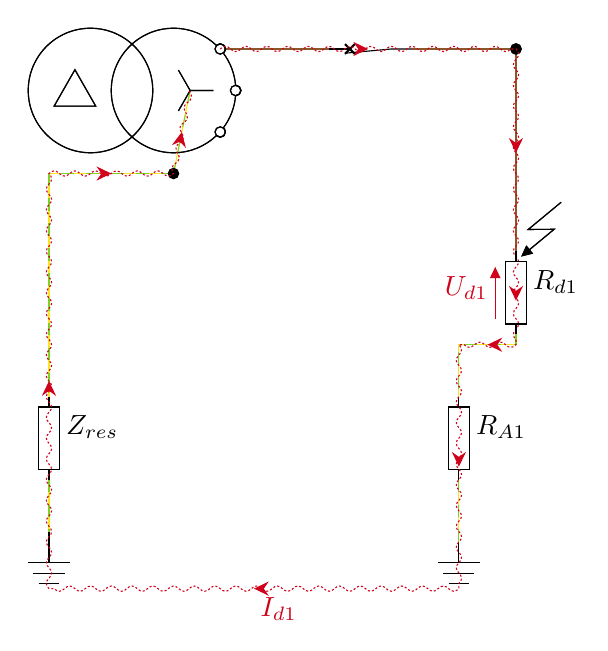
\begin{tikzpicture}[x=0.75pt,y=0.75pt,yscale=-1,xscale=1]
%uncomment if require: \path (0,313); %set diagram left start at 0, and has height of 313

%Straight Lines [id:da40140774002563195] 
\draw [color={rgb, 255:red, 248; green, 231; blue, 28 }  ,draw opacity=1 ]   (87.5,75) -- (27.5,75) -- (27.5,182.5) ;
%Straight Lines [id:da7768656062968136] 
\draw [color={rgb, 255:red, 248; green, 231; blue, 28 }  ,draw opacity=1 ]   (95.5,35) -- (87.5,75) ;
%Straight Lines [id:da0702550211386399] 
\draw [color={rgb, 255:red, 126; green, 211; blue, 33 }  ,draw opacity=1 ] [dash pattern={on 4.5pt off 4.5pt}]  (95.5,35) -- (87.5,75) ;
%Shape: Path Data [id:dp6564394705196642] 
\draw   (112.5,55) .. controls (112.5,56.38) and (111.38,57.5) .. (110,57.5) .. controls (109.29,57.5) and (108.65,57.2) .. (108.19,56.72) .. controls (102.81,61.85) and (95.52,65) .. (87.5,65) .. controls (70.93,65) and (57.5,51.57) .. (57.5,35) .. controls (57.5,18.43) and (70.93,5) .. (87.5,5) .. controls (95.52,5) and (102.81,8.15) .. (108.19,13.28) .. controls (108.65,12.8) and (109.29,12.5) .. (110,12.5) .. controls (111.38,12.5) and (112.5,13.62) .. (112.5,15) .. controls (112.5,15.82) and (112.11,16.54) .. (111.5,17) .. controls (114.8,21.39) and (116.92,26.71) .. (117.4,32.5) .. controls (117.43,32.5) and (117.47,32.5) .. (117.5,32.5) .. controls (118.88,32.5) and (120,33.62) .. (120,35) .. controls (120,36.38) and (118.88,37.5) .. (117.5,37.5) .. controls (117.47,37.5) and (117.43,37.5) .. (117.4,37.5) .. controls (116.92,43.29) and (114.8,48.61) .. (111.5,53) .. controls (112.11,53.46) and (112.5,54.18) .. (112.5,55) -- cycle ;
%Shape: Circle [id:dp6837865910950578] 
\draw   (17.5,35) .. controls (17.5,18.43) and (30.93,5) .. (47.5,5) .. controls (64.07,5) and (77.5,18.43) .. (77.5,35) .. controls (77.5,51.57) and (64.07,65) .. (47.5,65) .. controls (30.93,65) and (17.5,51.57) .. (17.5,35) -- cycle ;
%Shape: Triangle [id:dp4328019700995849] 
\draw   (40,25) -- (30,42.5) -- (50,42.5) -- cycle ;
%Shape: Star [id:dp9996543744584487] 
\draw   (106.75,35) -- (95.5,35) -- (89.88,44.81) -- (95.5,35) -- (89.88,25.19) -- (95.5,35) -- cycle ;
%Shape: Circle [id:dp4765432529475536] 
\draw   (107.5,15) .. controls (107.5,13.62) and (108.62,12.5) .. (110,12.5) .. controls (111.38,12.5) and (112.5,13.62) .. (112.5,15) .. controls (112.5,16.38) and (111.38,17.5) .. (110,17.5) .. controls (108.62,17.5) and (107.5,16.38) .. (107.5,15) -- cycle ;
%Shape: Circle [id:dp7950957606894842] 
\draw   (114.9,35) .. controls (114.9,33.62) and (116.02,32.5) .. (117.4,32.5) .. controls (118.78,32.5) and (119.9,33.62) .. (119.9,35) .. controls (119.9,36.38) and (118.78,37.5) .. (117.4,37.5) .. controls (116.02,37.5) and (114.9,36.38) .. (114.9,35) -- cycle ;
%Shape: Circle [id:dp47024921818209997] 
\draw   (107.5,55) .. controls (107.5,53.62) and (108.62,52.5) .. (110,52.5) .. controls (111.38,52.5) and (112.5,53.62) .. (112.5,55) .. controls (112.5,56.38) and (111.38,57.5) .. (110,57.5) .. controls (108.62,57.5) and (107.5,56.38) .. (107.5,55) -- cycle ;

%Straight Lines [id:da21818556641513764] 
\draw [color={rgb, 255:red, 139; green, 87; blue, 42 }  ,draw opacity=1 ]   (252.5,112.5) -- (252.5,17.5) ;
%Straight Lines [id:da8686907197740312] 
\draw [color={rgb, 255:red, 248; green, 231; blue, 28 }  ,draw opacity=1 ]   (225,222.5) -- (225,247.5) ;
%Straight Lines [id:da4369452606894554] 
\draw    (225,247.5) -- (225,262.5) ;
%Straight Lines [id:da41347797921121543] 
\draw    (215,262.5) -- (235,262.5) ;
%Straight Lines [id:da39005220989882616] 
\draw    (217.5,267.5) -- (232.5,267.5) ;
%Straight Lines [id:da04530437508662333] 
\draw    (220,272.5) -- (230,272.5) ;

%Straight Lines [id:da758878567860916] 
\draw [color={rgb, 255:red, 126; green, 211; blue, 33 }  ,draw opacity=1 ] [dash pattern={on 4.5pt off 4.5pt}]  (225,222.5) -- (225,247.5) ;
%Straight Lines [id:da7282446695874194] 
\draw    (225,217.5) -- (225,222.5) ;
%Shape: Rectangle [id:dp5377265306575283] 
\draw   (230,187.5) -- (230,217.5) -- (220,217.5) -- (220,187.5) -- cycle ;
%Straight Lines [id:da6172743564243196] 
\draw    (225,182.5) -- (225,187.5) ;

%Shape: Circle [id:dp9518184334454515] 
\draw  [fill={rgb, 255:red, 0; green, 0; blue, 0 }  ,fill opacity=1 ] (250,15) .. controls (250,13.62) and (251.12,12.5) .. (252.5,12.5) .. controls (253.88,12.5) and (255,13.62) .. (255,15) .. controls (255,16.38) and (253.88,17.5) .. (252.5,17.5) .. controls (251.12,17.5) and (250,16.38) .. (250,15) -- cycle ;
%Straight Lines [id:da698344453228456] 
\draw [color={rgb, 255:red, 139; green, 87; blue, 42 }  ,draw opacity=1 ]   (112.5,15) -- (162.5,15) ;
%Straight Lines [id:da3888199822065723] 
\draw [color={rgb, 255:red, 126; green, 211; blue, 33 }  ,draw opacity=1 ] [dash pattern={on 4.5pt off 4.5pt}]  (87.5,75) -- (27.5,75) -- (27.5,182.5) ;
%Straight Lines [id:da9929118367256647] 
\draw    (27.5,217.5) -- (27.5,222.5) ;
%Shape: Rectangle [id:dp5522927597315069] 
\draw   (32.5,187.5) -- (32.5,217.5) -- (22.5,217.5) -- (22.5,187.5) -- cycle ;
%Straight Lines [id:da51565112690186] 
\draw    (27.5,182.5) -- (27.5,187.5) ;

%Straight Lines [id:da20200008374801148] 
\draw [color={rgb, 255:red, 248; green, 231; blue, 28 }  ,draw opacity=1 ]   (27.5,222.5) -- (27.5,247.5) ;
%Straight Lines [id:da246860902568655] 
\draw [color={rgb, 255:red, 126; green, 211; blue, 33 }  ,draw opacity=1 ] [dash pattern={on 4.5pt off 4.5pt}]  (27.5,222.5) -- (27.5,247.5) ;
%Straight Lines [id:da8847595831515674] 
\draw    (27.5,247.5) -- (27.5,262.5) ;
%Straight Lines [id:da388525152974063] 
\draw    (17.5,262.5) -- (37.5,262.5) ;
%Straight Lines [id:da5307482611563814] 
\draw    (20,267.5) -- (35,267.5) ;
%Straight Lines [id:da879280977386573] 
\draw    (22.5,272.5) -- (32.5,272.5) ;

%Shape: Circle [id:dp23726887554171172] 
\draw  [fill={rgb, 255:red, 0; green, 0; blue, 0 }  ,fill opacity=1 ] (85,75) .. controls (85,73.62) and (86.12,72.5) .. (87.5,72.5) .. controls (88.88,72.5) and (90,73.62) .. (90,75) .. controls (90,76.38) and (88.88,77.5) .. (87.5,77.5) .. controls (86.12,77.5) and (85,76.38) .. (85,75) -- cycle ;
%Shape: Boxed Line [id:dp0646171917121674] 
\draw    (274.27,88.83) -- (258.39,101.97) -- (270.89,101.86) -- (257.31,113.09) ;
\draw [shift={(255,115)}, rotate = 320.40999999999997] [fill={rgb, 255:red, 0; green, 0; blue, 0 }  ][line width=0.08]  [draw opacity=0] (5.36,-2.57) -- (0,0) -- (5.36,2.57) -- cycle    ;
%Straight Lines [id:da0893199801246688] 
\draw    (170.5,17) -- (192.5,15) -- (202.5,15) ;
%Straight Lines [id:da4465712907894863] 
\draw    (172.5,15) -- (162.5,15) ;
\draw [shift={(172.5,15)}, rotate = 225] [color={rgb, 255:red, 0; green, 0; blue, 0 }  ][line width=0.75]    (-3.35,0) -- (3.35,0)(0,3.35) -- (0,-3.35)   ;

%Straight Lines [id:da6575503286927553] 
\draw [color={rgb, 255:red, 248; green, 231; blue, 28 }  ,draw opacity=1 ]   (252.5,152.5) -- (252.5,157.5) -- (225,157.5) -- (225,182.5) ;
%Straight Lines [id:da4804418012067295] 
\draw [color={rgb, 255:red, 139; green, 87; blue, 42 }  ,draw opacity=1 ]   (112.5,15) -- (162.5,15) ;
%Straight Lines [id:da7896587451085693] 
\draw [color={rgb, 255:red, 139; green, 87; blue, 42 }  ,draw opacity=1 ]   (202.5,15) -- (252.5,15) ;
%Shape: Path Data [id:dp195065302202169] 
\draw   (112.5,55) .. controls (112.5,56.38) and (111.38,57.5) .. (110,57.5) .. controls (109.29,57.5) and (108.65,57.2) .. (108.19,56.72) .. controls (102.81,61.85) and (95.52,65) .. (87.5,65) .. controls (70.93,65) and (57.5,51.57) .. (57.5,35) .. controls (57.5,18.43) and (70.93,5) .. (87.5,5) .. controls (95.52,5) and (102.81,8.15) .. (108.19,13.28) .. controls (108.65,12.8) and (109.29,12.5) .. (110,12.5) .. controls (111.38,12.5) and (112.5,13.62) .. (112.5,15) .. controls (112.5,15.82) and (112.11,16.54) .. (111.5,17) .. controls (114.8,21.39) and (116.92,26.71) .. (117.4,32.5) .. controls (117.43,32.5) and (117.47,32.5) .. (117.5,32.5) .. controls (118.88,32.5) and (120,33.62) .. (120,35) .. controls (120,36.38) and (118.88,37.5) .. (117.5,37.5) .. controls (117.47,37.5) and (117.43,37.5) .. (117.4,37.5) .. controls (116.92,43.29) and (114.8,48.61) .. (111.5,53) .. controls (112.11,53.46) and (112.5,54.18) .. (112.5,55) -- cycle ;
%Shape: Circle [id:dp10449815547230978] 
\draw   (17.5,35) .. controls (17.5,18.43) and (30.93,5) .. (47.5,5) .. controls (64.07,5) and (77.5,18.43) .. (77.5,35) .. controls (77.5,51.57) and (64.07,65) .. (47.5,65) .. controls (30.93,65) and (17.5,51.57) .. (17.5,35) -- cycle ;
%Shape: Triangle [id:dp13602835689186588] 
\draw   (40,25) -- (30,42.5) -- (50,42.5) -- cycle ;
%Shape: Star [id:dp5246434088790826] 
\draw   (106.75,35) -- (95.5,35) -- (89.88,44.81) -- (95.5,35) -- (89.88,25.19) -- (95.5,35) -- cycle ;
%Shape: Circle [id:dp3622486105745091] 
\draw   (107.5,15) .. controls (107.5,13.62) and (108.62,12.5) .. (110,12.5) .. controls (111.38,12.5) and (112.5,13.62) .. (112.5,15) .. controls (112.5,16.38) and (111.38,17.5) .. (110,17.5) .. controls (108.62,17.5) and (107.5,16.38) .. (107.5,15) -- cycle ;
%Shape: Circle [id:dp7116693252528491] 
\draw   (114.9,35) .. controls (114.9,33.62) and (116.02,32.5) .. (117.4,32.5) .. controls (118.78,32.5) and (119.9,33.62) .. (119.9,35) .. controls (119.9,36.38) and (118.78,37.5) .. (117.4,37.5) .. controls (116.02,37.5) and (114.9,36.38) .. (114.9,35) -- cycle ;
%Shape: Circle [id:dp18972999107641209] 
\draw   (107.5,55) .. controls (107.5,53.62) and (108.62,52.5) .. (110,52.5) .. controls (111.38,52.5) and (112.5,53.62) .. (112.5,55) .. controls (112.5,56.38) and (111.38,57.5) .. (110,57.5) .. controls (108.62,57.5) and (107.5,56.38) .. (107.5,55) -- cycle ;

%Straight Lines [id:da014549812099070136] 
\draw [color={rgb, 255:red, 139; green, 87; blue, 42 }  ,draw opacity=1 ]   (252.5,112.5) -- (252.5,17.5) ;
%Straight Lines [id:da26084750256284417] 
\draw [color={rgb, 255:red, 126; green, 211; blue, 33 }  ,draw opacity=1 ] [dash pattern={on 4.5pt off 4.5pt}]  (252.5,152.5) -- (252.5,157.5) -- (225,157.5) -- (225,182.5) ;
%Straight Lines [id:da3030992302203893] 
\draw [color={rgb, 255:red, 248; green, 231; blue, 28 }  ,draw opacity=1 ]   (225,222.5) -- (225,252.5) ;
%Straight Lines [id:da15920917753755837] 
\draw [color={rgb, 255:red, 126; green, 211; blue, 33 }  ,draw opacity=1 ] [dash pattern={on 4.5pt off 4.5pt}]  (225,222.5) -- (225,252.5) ;
%Shape: Circle [id:dp17133751283477605] 
\draw  [fill={rgb, 255:red, 0; green, 0; blue, 0 }  ,fill opacity=1 ] (250,15) .. controls (250,13.62) and (251.12,12.5) .. (252.5,12.5) .. controls (253.88,12.5) and (255,13.62) .. (255,15) .. controls (255,16.38) and (253.88,17.5) .. (252.5,17.5) .. controls (251.12,17.5) and (250,16.38) .. (250,15) -- cycle ;
%Shape: Boxed Line [id:dp8068084114642486] 
\draw    (274.27,88.83) -- (258.39,101.97) -- (270.89,101.86) -- (257.31,113.09) ;
\draw [shift={(255,115)}, rotate = 320.40999999999997] [fill={rgb, 255:red, 0; green, 0; blue, 0 }  ][line width=0.08]  [draw opacity=0] (5.36,-2.57) -- (0,0) -- (5.36,2.57) -- cycle    ;
%Straight Lines [id:da21551575051470273] 
\draw [color={rgb, 255:red, 208; green, 2; blue, 27 }  ,draw opacity=1 ] [dash pattern={on 0.75pt off 0.75pt}]  (110,15) .. controls (111.67,13.33) and (113.33,13.33) .. (115,15) .. controls (116.67,16.67) and (118.33,16.67) .. (120,15) .. controls (121.67,13.33) and (123.33,13.33) .. (125,15) .. controls (126.67,16.67) and (128.33,16.67) .. (130,15) .. controls (131.67,13.33) and (133.33,13.33) .. (135,15) .. controls (136.67,16.67) and (138.33,16.67) .. (140,15) .. controls (141.67,13.33) and (143.33,13.33) .. (145,15) .. controls (146.67,16.67) and (148.33,16.67) .. (150,15) .. controls (151.67,13.33) and (153.33,13.33) .. (155,15) .. controls (156.67,16.67) and (158.33,16.67) .. (160,15) .. controls (161.67,13.33) and (163.33,13.33) .. (165,15) .. controls (166.67,16.67) and (168.33,16.67) .. (170,15) .. controls (171.67,13.33) and (173.33,13.33) .. (175,15) .. controls (176.67,16.67) and (178.33,16.67) .. (180,15) .. controls (181.67,13.33) and (183.33,13.33) .. (185,15) .. controls (186.67,16.67) and (188.33,16.67) .. (190,15) .. controls (191.67,13.33) and (193.33,13.33) .. (195,15) .. controls (196.67,16.67) and (198.33,16.67) .. (200,15) .. controls (201.67,13.33) and (203.33,13.33) .. (205,15) .. controls (206.67,16.67) and (208.33,16.67) .. (210,15) .. controls (211.67,13.33) and (213.33,13.33) .. (215,15) .. controls (216.67,16.67) and (218.33,16.67) .. (220,15) .. controls (221.67,13.33) and (223.33,13.33) .. (225,15) .. controls (226.67,16.67) and (228.33,16.67) .. (230,15) .. controls (231.67,13.33) and (233.33,13.33) .. (235,15) .. controls (236.67,16.67) and (238.33,16.67) .. (240,15) .. controls (241.67,13.33) and (243.33,13.33) .. (245,15) .. controls (246.67,16.67) and (248.33,16.67) .. (250,15) -- (252.5,15) -- (252.5,15) .. controls (254.17,16.67) and (254.17,18.33) .. (252.5,20) .. controls (250.83,21.67) and (250.83,23.33) .. (252.5,25) .. controls (254.17,26.67) and (254.17,28.33) .. (252.5,30) .. controls (250.83,31.67) and (250.83,33.33) .. (252.5,35) .. controls (254.17,36.67) and (254.17,38.33) .. (252.5,40) .. controls (250.83,41.67) and (250.83,43.33) .. (252.5,45) .. controls (254.17,46.67) and (254.17,48.33) .. (252.5,50) .. controls (250.83,51.67) and (250.83,53.33) .. (252.5,55) .. controls (254.17,56.67) and (254.17,58.33) .. (252.5,60) .. controls (250.83,61.67) and (250.83,63.33) .. (252.5,65) .. controls (254.17,66.67) and (254.17,68.33) .. (252.5,70) .. controls (250.83,71.67) and (250.83,73.33) .. (252.5,75) .. controls (254.17,76.67) and (254.17,78.33) .. (252.5,80) .. controls (250.83,81.67) and (250.83,83.33) .. (252.5,85) .. controls (254.17,86.67) and (254.17,88.33) .. (252.5,90) .. controls (250.83,91.67) and (250.83,93.33) .. (252.5,95) .. controls (254.17,96.67) and (254.17,98.33) .. (252.5,100) .. controls (250.83,101.67) and (250.83,103.33) .. (252.5,105) .. controls (254.17,106.67) and (254.17,108.33) .. (252.5,110) .. controls (250.83,111.67) and (250.83,113.33) .. (252.5,115) -- (252.5,115) .. controls (254.17,116.67) and (254.17,118.33) .. (252.5,120) .. controls (250.83,121.67) and (250.83,123.33) .. (252.5,125) .. controls (254.17,126.67) and (254.17,128.33) .. (252.5,130) .. controls (250.83,131.67) and (250.83,133.33) .. (252.5,135) .. controls (254.17,136.67) and (254.17,138.33) .. (252.5,140) .. controls (250.83,141.67) and (250.83,143.33) .. (252.5,145) .. controls (254.17,146.67) and (254.17,148.33) .. (252.5,150) .. controls (250.83,151.67) and (250.83,153.33) .. (252.5,155) -- (252.5,157.5) -- (252.5,157.5) .. controls (250.83,159.17) and (249.17,159.17) .. (247.5,157.5) .. controls (245.83,155.83) and (244.17,155.83) .. (242.5,157.5) .. controls (240.83,159.17) and (239.17,159.17) .. (237.5,157.5) .. controls (235.83,155.83) and (234.17,155.83) .. (232.5,157.5) .. controls (230.83,159.17) and (229.17,159.17) .. (227.5,157.5) -- (225,157.5) -- (225,157.5) .. controls (226.67,159.17) and (226.67,160.83) .. (225,162.5) .. controls (223.33,164.17) and (223.33,165.83) .. (225,167.5) .. controls (226.67,169.17) and (226.67,170.83) .. (225,172.5) .. controls (223.33,174.17) and (223.33,175.83) .. (225,177.5) .. controls (226.67,179.17) and (226.67,180.83) .. (225,182.5) .. controls (223.33,184.17) and (223.33,185.83) .. (225,187.5) .. controls (226.67,189.17) and (226.67,190.83) .. (225,192.5) .. controls (223.33,194.17) and (223.33,195.83) .. (225,197.5) .. controls (226.67,199.17) and (226.67,200.83) .. (225,202.5) .. controls (223.33,204.17) and (223.33,205.83) .. (225,207.5) .. controls (226.67,209.17) and (226.67,210.83) .. (225,212.5) .. controls (223.33,214.17) and (223.33,215.83) .. (225,217.5) .. controls (226.67,219.17) and (226.67,220.83) .. (225,222.5) .. controls (223.33,224.17) and (223.33,225.83) .. (225,227.5) .. controls (226.67,229.17) and (226.67,230.83) .. (225,232.5) .. controls (223.33,234.17) and (223.33,235.83) .. (225,237.5) .. controls (226.67,239.17) and (226.67,240.83) .. (225,242.5) .. controls (223.33,244.17) and (223.33,245.83) .. (225,247.5) .. controls (226.67,249.17) and (226.67,250.83) .. (225,252.5) .. controls (223.33,254.17) and (223.33,255.83) .. (225,257.5) .. controls (226.67,259.17) and (226.67,260.83) .. (225,262.5) .. controls (223.33,264.17) and (223.33,265.83) .. (225,267.5) .. controls (226.67,269.17) and (226.67,270.83) .. (225,272.5) -- (225,275) -- (225,275) .. controls (223.33,276.67) and (221.67,276.67) .. (220,275) .. controls (218.33,273.33) and (216.67,273.33) .. (215,275) .. controls (213.33,276.67) and (211.67,276.67) .. (210,275) .. controls (208.33,273.33) and (206.67,273.33) .. (205,275) .. controls (203.33,276.67) and (201.67,276.67) .. (200,275) .. controls (198.33,273.33) and (196.67,273.33) .. (195,275) .. controls (193.33,276.67) and (191.67,276.67) .. (190,275) .. controls (188.33,273.33) and (186.67,273.33) .. (185,275) .. controls (183.33,276.67) and (181.67,276.67) .. (180,275) .. controls (178.33,273.33) and (176.67,273.33) .. (175,275) .. controls (173.33,276.67) and (171.67,276.67) .. (170,275) .. controls (168.33,273.33) and (166.67,273.33) .. (165,275) .. controls (163.33,276.67) and (161.67,276.67) .. (160,275) .. controls (158.33,273.33) and (156.67,273.33) .. (155,275) .. controls (153.33,276.67) and (151.67,276.67) .. (150,275) .. controls (148.33,273.33) and (146.67,273.33) .. (145,275) .. controls (143.33,276.67) and (141.67,276.67) .. (140,275) .. controls (138.33,273.33) and (136.67,273.33) .. (135,275) .. controls (133.33,276.67) and (131.67,276.67) .. (130,275) .. controls (128.33,273.33) and (126.67,273.33) .. (125,275) .. controls (123.33,276.67) and (121.67,276.67) .. (120,275) .. controls (118.33,273.33) and (116.67,273.33) .. (115,275) .. controls (113.33,276.67) and (111.67,276.67) .. (110,275) .. controls (108.33,273.33) and (106.67,273.33) .. (105,275) .. controls (103.33,276.67) and (101.67,276.67) .. (100,275) .. controls (98.33,273.33) and (96.67,273.33) .. (95,275) .. controls (93.33,276.67) and (91.67,276.67) .. (90,275) .. controls (88.33,273.33) and (86.67,273.33) .. (85,275) .. controls (83.33,276.67) and (81.67,276.67) .. (80,275) .. controls (78.33,273.33) and (76.67,273.33) .. (75,275) .. controls (73.33,276.67) and (71.67,276.67) .. (70,275) .. controls (68.33,273.33) and (66.67,273.33) .. (65,275) .. controls (63.33,276.67) and (61.67,276.67) .. (60,275) .. controls (58.33,273.33) and (56.67,273.33) .. (55,275) .. controls (53.33,276.67) and (51.67,276.67) .. (50,275) .. controls (48.33,273.33) and (46.67,273.33) .. (45,275) .. controls (43.33,276.67) and (41.67,276.67) .. (40,275) .. controls (38.33,273.33) and (36.67,273.33) .. (35,275) .. controls (33.33,276.67) and (31.67,276.67) .. (30,275) -- (27.5,275) -- (27.5,275) .. controls (25.83,273.33) and (25.83,271.67) .. (27.5,270) .. controls (29.17,268.33) and (29.17,266.67) .. (27.5,265) .. controls (25.83,263.33) and (25.83,261.67) .. (27.5,260) .. controls (29.17,258.33) and (29.17,256.67) .. (27.5,255) .. controls (25.83,253.33) and (25.83,251.67) .. (27.5,250) .. controls (29.17,248.33) and (29.17,246.67) .. (27.5,245) .. controls (25.83,243.33) and (25.83,241.67) .. (27.5,240) .. controls (29.17,238.33) and (29.17,236.67) .. (27.5,235) .. controls (25.83,233.33) and (25.83,231.67) .. (27.5,230) .. controls (29.17,228.33) and (29.17,226.67) .. (27.5,225) .. controls (25.83,223.33) and (25.83,221.67) .. (27.5,220) .. controls (29.17,218.33) and (29.17,216.67) .. (27.5,215) .. controls (25.83,213.33) and (25.83,211.67) .. (27.5,210) .. controls (29.17,208.33) and (29.17,206.67) .. (27.5,205) .. controls (25.83,203.33) and (25.83,201.67) .. (27.5,200) .. controls (29.17,198.33) and (29.17,196.67) .. (27.5,195) .. controls (25.83,193.33) and (25.83,191.67) .. (27.5,190) .. controls (29.17,188.33) and (29.17,186.67) .. (27.5,185) .. controls (25.83,183.33) and (25.83,181.67) .. (27.5,180) .. controls (29.17,178.33) and (29.17,176.67) .. (27.5,175) .. controls (25.83,173.33) and (25.83,171.67) .. (27.5,170) .. controls (29.17,168.33) and (29.17,166.67) .. (27.5,165) .. controls (25.83,163.33) and (25.83,161.67) .. (27.5,160) .. controls (29.17,158.33) and (29.17,156.67) .. (27.5,155) .. controls (25.83,153.33) and (25.83,151.67) .. (27.5,150) .. controls (29.17,148.33) and (29.17,146.67) .. (27.5,145) .. controls (25.83,143.33) and (25.83,141.67) .. (27.5,140) .. controls (29.17,138.33) and (29.17,136.67) .. (27.5,135) .. controls (25.83,133.33) and (25.83,131.67) .. (27.5,130) .. controls (29.17,128.33) and (29.17,126.67) .. (27.5,125) .. controls (25.83,123.33) and (25.83,121.67) .. (27.5,120) .. controls (29.17,118.33) and (29.17,116.67) .. (27.5,115) .. controls (25.83,113.33) and (25.83,111.67) .. (27.5,110) .. controls (29.17,108.33) and (29.17,106.67) .. (27.5,105) .. controls (25.83,103.33) and (25.83,101.67) .. (27.5,100) .. controls (29.17,98.33) and (29.17,96.67) .. (27.5,95) .. controls (25.83,93.33) and (25.83,91.67) .. (27.5,90) .. controls (29.17,88.33) and (29.17,86.67) .. (27.5,85) .. controls (25.83,83.33) and (25.83,81.67) .. (27.5,80) .. controls (29.17,78.33) and (29.17,76.67) .. (27.5,75) -- (27.5,75) .. controls (29.17,73.33) and (30.83,73.33) .. (32.5,75) .. controls (34.17,76.67) and (35.83,76.67) .. (37.5,75) .. controls (39.17,73.33) and (40.83,73.33) .. (42.5,75) .. controls (44.17,76.67) and (45.83,76.67) .. (47.5,75) .. controls (49.17,73.33) and (50.83,73.33) .. (52.5,75) .. controls (54.17,76.67) and (55.83,76.67) .. (57.5,75) .. controls (59.17,73.33) and (60.83,73.33) .. (62.5,75) .. controls (64.17,76.67) and (65.83,76.67) .. (67.5,75) .. controls (69.17,73.33) and (70.83,73.33) .. (72.5,75) .. controls (74.17,76.67) and (75.83,76.67) .. (77.5,75) .. controls (79.17,73.33) and (80.83,73.33) .. (82.5,75) .. controls (84.17,76.67) and (85.83,76.67) .. (87.5,75) -- (87.5,75) .. controls (86.19,73.04) and (86.52,71.41) .. (88.48,70.1) .. controls (90.44,68.79) and (90.77,67.15) .. (89.46,65.19) .. controls (88.15,63.23) and (88.48,61.6) .. (90.44,60.29) .. controls (92.4,58.98) and (92.73,57.35) .. (91.42,55.39) .. controls (90.11,53.43) and (90.44,51.8) .. (92.4,50.49) .. controls (94.36,49.18) and (94.69,47.54) .. (93.38,45.58) .. controls (92.07,43.62) and (92.4,41.99) .. (94.36,40.68) .. controls (96.32,39.37) and (96.65,37.74) .. (95.34,35.78) -- (95.5,35) -- (95.5,35) ;
\draw [shift={(181.25,15)}, rotate = 180] [fill={rgb, 255:red, 208; green, 2; blue, 27 }  ,fill opacity=1 ][line width=0.08]  [draw opacity=0] (7.14,-3.43) -- (0,0) -- (7.14,3.43) -- (4.74,0) -- cycle    ;
\draw [shift={(252.5,65)}, rotate = 270] [fill={rgb, 255:red, 208; green, 2; blue, 27 }  ,fill opacity=1 ][line width=0.08]  [draw opacity=0] (7.14,-3.43) -- (0,0) -- (7.14,3.43) -- (4.74,0) -- cycle    ;
\draw [shift={(252.5,136.25)}, rotate = 270] [fill={rgb, 255:red, 208; green, 2; blue, 27 }  ,fill opacity=1 ][line width=0.08]  [draw opacity=0] (7.14,-3.43) -- (0,0) -- (7.14,3.43) -- (4.74,0) -- cycle    ;
\draw [shift={(238.75,157.5)}, rotate = 360] [fill={rgb, 255:red, 208; green, 2; blue, 27 }  ,fill opacity=1 ][line width=0.08]  [draw opacity=0] (7.14,-3.43) -- (0,0) -- (7.14,3.43) -- (4.74,0) -- cycle    ;
\draw [shift={(225,216.25)}, rotate = 270] [fill={rgb, 255:red, 208; green, 2; blue, 27 }  ,fill opacity=1 ][line width=0.08]  [draw opacity=0] (7.14,-3.43) -- (0,0) -- (7.14,3.43) -- (4.74,0) -- cycle    ;
\draw [shift={(126.25,275)}, rotate = 360] [fill={rgb, 255:red, 208; green, 2; blue, 27 }  ,fill opacity=1 ][line width=0.08]  [draw opacity=0] (7.14,-3.43) -- (0,0) -- (7.14,3.43) -- (4.74,0) -- cycle    ;
\draw [shift={(27.5,175)}, rotate = 450] [fill={rgb, 255:red, 208; green, 2; blue, 27 }  ,fill opacity=1 ][line width=0.08]  [draw opacity=0] (7.14,-3.43) -- (0,0) -- (7.14,3.43) -- (4.74,0) -- cycle    ;
\draw [shift={(57.5,75)}, rotate = 180] [fill={rgb, 255:red, 208; green, 2; blue, 27 }  ,fill opacity=1 ][line width=0.08]  [draw opacity=0] (7.14,-3.43) -- (0,0) -- (7.14,3.43) -- (4.74,0) -- cycle    ;
\draw [shift={(91.5,55)}, rotate = 461.31] [fill={rgb, 255:red, 208; green, 2; blue, 27 }  ,fill opacity=1 ][line width=0.08]  [draw opacity=0] (7.14,-3.43) -- (0,0) -- (7.14,3.43) -- (4.74,0) -- cycle    ;
%Straight Lines [id:da5878987587379367] 
\draw    (252.5,147.5) -- (252.5,152.5) ;
%Shape: Rectangle [id:dp5233395725568003] 
\draw   (257.5,117.5) -- (257.5,147.5) -- (247.5,147.5) -- (247.5,117.5) -- cycle ;
%Straight Lines [id:da6884797067797518] 
\draw    (252.5,112.5) -- (252.5,117.5) ;

%Straight Lines [id:da07071854927031873] 
\draw [color={rgb, 255:red, 208; green, 2; blue, 27 }  ,draw opacity=1 ]   (242.5,123) -- (242.5,145) ;
\draw [shift={(242.5,120)}, rotate = 90] [fill={rgb, 255:red, 208; green, 2; blue, 27 }  ,fill opacity=1 ][line width=0.08]  [draw opacity=0] (5.36,-2.57) -- (0,0) -- (5.36,2.57) -- cycle    ;

% Text Node
\draw (232,190.5) node [anchor=north west][inner sep=0.75pt]   [align=left] {$R_{A1}$};
% Text Node
\draw (34.5,190.5) node [anchor=north west][inner sep=0.75pt]   [align=left] {$Z_{res}$};
% Text Node
\draw (128.25,278) node [anchor=north west][inner sep=0.75pt]  [color={rgb, 255:red, 208; green, 2; blue, 27 }  ,opacity=1 ] [align=left] {$I_{d1}$};
% Text Node
\draw (217,123.5) node [anchor=north west][inner sep=0.75pt]  [color={rgb, 255:red, 208; green, 2; blue, 27 }  ,opacity=1 ] [align=left] {$U_{d1}$};
% Text Node
\draw (259.5,120.5) node [anchor=north west][inner sep=0.75pt]   [align=left] {$R_{d1}$};


\end{tikzpicture}
\end{figure}

%\end{document}


L'intensité de courant $I_d1$ vaut alors :
\begin{formule}[Courant du premier défaut $I_d1$ en schéma Isolé-Individuel]
\begin{align*}
		I_d &= \frac{U_{0}}{Z_{res}+R_{A1}+R_{d1}}
\end{align*}
\end{formule}

\begin{textvariables}
U_{0}						& tension nominale simple						& volt			& \volt					& 	Différence de potentiel entre les masses métalliques et la terre 	\\
Z_{res}						& impédance											& ohm			& \ohm					& 	Impédance de fuite $Z_res$ du réseau électrique 	\\
R_{A1}						& résistance											& ohm			& \ohm					& 	Résistance de la prise de terre de l'appareil 1 	\\
R_{d1}						& résistance											& ohm			& \ohm					& 	Résistance de défaut 	d'isolement de l'appareil 1\\
\end{textvariables}

Le courant de défaut $I_{d1}$ fera alors apparaître une \emph{tension de défaut} $U_{d1}$ entre la masse métallique de l'appareil 1 et la terre. Cette tension, limitée par l'impédance de fuite, sera très largement inférieure à  $U_L$ et ne sera donc pas dangereuse. La situation sera similaire avec un schéma Impédant-Individuel $Z_N$, ou l'impédance de limitation limitera également le courant de défaut :

\begin{formule}[Tension de défaut $U_{d1}$ en schéma Isolé-Individuel]
\begin{align*}
		U_{d1} &= R_{A1} \times I_{d1} \\
			   &\ll	 U_L
\end{align*}
\end{formule}

\begin{textvariables}
R_{A1}						& résistance											& ohm			& \ohm					& 	Résistance de la prise de terre de l'appareil 1 	\\
I_{d1}							& intensité							& ampère		& \ampere				& 	Courant de défaut de l'appareil 1\\
U_{L}						& tension							& volt			& \volt					& 	Tension de sécurité du local avec :
\begin{description}[nosep, leftmargin=*]
\item[Local sec :] $U_{L}=\SI{50}{\volt}$
\item[Local humide :] $U_{L}=\SI{25}{\volt}$
\end{description} \\
\end{textvariables}

Le fonctionnement d'un schéma IT sera également identique au premier défaut, que les masses soient interconnectées ou individuellement raccordées à la terre.

\begin{exemple}[Tension de défaut $U_{d1}$ en schéma Isolé-Individuel au premier défaut]
Si on considère que le transformateur est un transformateur $\SI{20}{\kilo\volt}/\SI{400}{\volt}$, que $Z_{res}=\SI{3500}{\ohm}$, $R_{A1}=\SI{40}{\ohm}$ et que $R_d = \SI{2}{\ohm}$, on peut déduire que le courant de défaut $I_d$ vaut :
\begin{align*}
		I_{d1} &= \frac{U_{0}}{Z_{res}+R_{A1}+R_{d1}} \\
				&=\frac{400}{3500+40+2} \\
				&= \SI{64,9}{\milli\ampere} \\
\end{align*}
Si une personne touche à la masse du récepteur 1, elle sera soumise à une tension de défaut $U_{d1}$ :
\begin{align*}
		U_{d1} &= R_{A1} \times I_{d1} \\
				&=40 \times 0,0649 \\
				&= \SI{2,6}{\volt}
\end{align*}
\end{exemple}

Lors de l'apparition d'un deuxième défaut d'isolement sur un autre conducteur actif, un courant de défaut $I_{d2}$ va apparaitre. Celui-ci va s'apparenter à un court-circuit et de ce fait, $I_{d1}$ sera négligé. \\
Dans les calculs, il faut encore tenir compte de la \emph{résistance de défaut} $R_d$ qui prend en compte la nature du défaut d'isolement (franc ou non-franc) et les résistances des carcasses métalliques des appareils 1 et 2.\\

\begin{figure}[H]
\caption{Installation Isolé-Individuelle}
\begin{subfigure}[t]{0.49\linewidth}
%--------------------------------------
%ELECTROTECHNIQUE - SCHEMA DE LIAISON A LA TERRE
%--------------------------------------

%utiliser les environnement \begin{comment} \end{comment} pour mettre en commentaire le préambule une fois la programmation appelée dans le document maître (!ne pas oublier de mettre en commentaire \end{document}!)

\begin{comment}

\documentclass[a4paper, 11pt, twoside, fleqn]{memoir}

\usepackage{AOCDTF}

\marqueurchapitre
\decoupagechapitre{1} %juste pour éviter les erreurs lors de la compilation des sous-programmations (passera en commentaire)

%lien d'édition des figures Tikz sur le site mathcha.io (rajouter le lien d'une modification effectuée sur la figure tikz avec le nom du modificateur car il n'y a qu'un lien par compte)

%lien mathcha Bruno Douchy : https://www.mathcha.io/editor/DXXG1FgjiNJCe0yo2ZTqzEeM8hlg57ygtvk5Mpy

%--------------------------------------
%corps du document
%--------------------------------------

\begin{document} %corps du document
	\openleft %début de chapitre à gauche

\end{comment}


% Pattern Info
 
\tikzset{
pattern size/.store in=\mcSize, 
pattern size = 5pt,
pattern thickness/.store in=\mcThickness, 
pattern thickness = 0.3pt,
pattern radius/.store in=\mcRadius, 
pattern radius = 1pt}
\makeatletter
\pgfutil@ifundefined{pgf@pattern@name@_ynwbix4sg}{
\pgfdeclarepatternformonly[\mcThickness,\mcSize]{_ynwbix4sg}
{\pgfqpoint{0pt}{0pt}}
{\pgfpoint{\mcSize+\mcThickness}{\mcSize+\mcThickness}}
{\pgfpoint{\mcSize}{\mcSize}}
{
\pgfsetcolor{\tikz@pattern@color}
\pgfsetlinewidth{\mcThickness}
\pgfpathmoveto{\pgfqpoint{0pt}{0pt}}
\pgfpathlineto{\pgfpoint{\mcSize+\mcThickness}{\mcSize+\mcThickness}}
\pgfusepath{stroke}
}}
\makeatother
\tikzset{every picture/.style={line width=0.5pt}} %set default line width to 0.75pt        

\begin{tikzpicture}[x=0.75pt,y=0.75pt,yscale=-0.6,xscale=0.6]
%uncomment if require: \path (0,293); %set diagram left start at 0, and has height of 293

%Shape: Rectangle [id:dp7263765394963575] 
\draw  [dash pattern={on 2.25pt off 2.25pt on 1pt off 2.25pt}] (242.5,115) -- (302.5,115) -- (302.5,145) -- (242.5,145) -- cycle ;
%Shape: Rectangle [id:dp35881098160444513] 
\draw  [dash pattern={on 2.25pt off 2.25pt on 1pt off 2.25pt}] (327.5,115) -- (387.5,115) -- (387.5,145) -- (327.5,145) -- cycle ;
%Shape: Rectangle [id:dp6695507085328443] 
\draw  [dash pattern={on 2.25pt off 2.25pt on 1pt off 2.25pt}] (412.5,115) -- (472.5,115) -- (472.5,145) -- (412.5,145) -- cycle ;
%Straight Lines [id:da8040415491242667] 
\draw [color={rgb, 255:red, 74; green, 144; blue, 226 }  ,draw opacity=1 ]   (90,75) -- (162.5,75) ;
%Straight Lines [id:da39577632473002744] 
\draw [color={rgb, 255:red, 74; green, 144; blue, 226 }  ,draw opacity=1 ]   (202.5,75.5) -- (460,75) ;
%Straight Lines [id:da25678520536510285] 
\draw [color={rgb, 255:red, 248; green, 231; blue, 28 }  ,draw opacity=1 ]   (87.5,75) -- (27.5,75) -- (27.5,182.5) ;
%Straight Lines [id:da5402140347093166] 
\draw [color={rgb, 255:red, 248; green, 231; blue, 28 }  ,draw opacity=1 ]   (95.5,35) -- (87.5,75) -- (87.5,107.5) ;
%Straight Lines [id:da6572902402425455] 
\draw [color={rgb, 255:red, 126; green, 211; blue, 33 }  ,draw opacity=1 ] [dash pattern={on 2.25pt off 2.25pt}]  (95.5,35) -- (87.5,75) -- (87.5,107.5) ;
%Straight Lines [id:da06818694087843613] 
\draw [color={rgb, 255:red, 248; green, 231; blue, 28 }  ,draw opacity=1 ]   (240,135) -- (225,135) -- (225,182.5) ;
%Straight Lines [id:da43234765426393074] 
\draw    (202.5,35) -- (462.5,35) ;
%Straight Lines [id:da8191173199817187] 
\draw [color={rgb, 255:red, 139; green, 87; blue, 42 }  ,draw opacity=1 ]   (202.5,15) -- (462.5,15) ;
%Straight Lines [id:da3978846646736923] 
\draw [color={rgb, 255:red, 155; green, 155; blue, 155 }  ,draw opacity=1 ]   (202.5,55) -- (462.5,55) ;
%Shape: Path Data [id:dp12879159047606914] 
\draw   (112.5,55) .. controls (112.5,56.38) and (111.38,57.5) .. (110,57.5) .. controls (109.29,57.5) and (108.65,57.2) .. (108.19,56.72) .. controls (102.81,61.85) and (95.52,65) .. (87.5,65) .. controls (70.93,65) and (57.5,51.57) .. (57.5,35) .. controls (57.5,18.43) and (70.93,5) .. (87.5,5) .. controls (95.52,5) and (102.81,8.15) .. (108.19,13.28) .. controls (108.65,12.8) and (109.29,12.5) .. (110,12.5) .. controls (111.38,12.5) and (112.5,13.62) .. (112.5,15) .. controls (112.5,15.82) and (112.11,16.54) .. (111.5,17) .. controls (114.8,21.39) and (116.92,26.71) .. (117.4,32.5) .. controls (117.43,32.5) and (117.47,32.5) .. (117.5,32.5) .. controls (118.88,32.5) and (120,33.62) .. (120,35) .. controls (120,36.38) and (118.88,37.5) .. (117.5,37.5) .. controls (117.47,37.5) and (117.43,37.5) .. (117.4,37.5) .. controls (116.92,43.29) and (114.8,48.61) .. (111.5,53) .. controls (112.11,53.46) and (112.5,54.18) .. (112.5,55) -- cycle ;
%Shape: Circle [id:dp3480809900403856] 
\draw   (17.5,35) .. controls (17.5,18.43) and (30.93,5) .. (47.5,5) .. controls (64.07,5) and (77.5,18.43) .. (77.5,35) .. controls (77.5,51.57) and (64.07,65) .. (47.5,65) .. controls (30.93,65) and (17.5,51.57) .. (17.5,35) -- cycle ;
%Shape: Triangle [id:dp8604762228071411] 
\draw   (40,25) -- (30,42.5) -- (50,42.5) -- cycle ;
%Shape: Star [id:dp8212895262481444] 
\draw   (106.75,35) -- (95.5,35) -- (89.88,44.81) -- (95.5,35) -- (89.88,25.19) -- (95.5,35) -- cycle ;
%Shape: Circle [id:dp6479761831984828] 
\draw   (107.5,15) .. controls (107.5,13.62) and (108.62,12.5) .. (110,12.5) .. controls (111.38,12.5) and (112.5,13.62) .. (112.5,15) .. controls (112.5,16.38) and (111.38,17.5) .. (110,17.5) .. controls (108.62,17.5) and (107.5,16.38) .. (107.5,15) -- cycle ;
%Shape: Circle [id:dp9340435311488099] 
\draw   (114.9,35) .. controls (114.9,33.62) and (116.02,32.5) .. (117.4,32.5) .. controls (118.78,32.5) and (119.9,33.62) .. (119.9,35) .. controls (119.9,36.38) and (118.78,37.5) .. (117.4,37.5) .. controls (116.02,37.5) and (114.9,36.38) .. (114.9,35) -- cycle ;
%Shape: Circle [id:dp10166063766932587] 
\draw   (107.5,55) .. controls (107.5,53.62) and (108.62,52.5) .. (110,52.5) .. controls (111.38,52.5) and (112.5,53.62) .. (112.5,55) .. controls (112.5,56.38) and (111.38,57.5) .. (110,57.5) .. controls (108.62,57.5) and (107.5,56.38) .. (107.5,55) -- cycle ;

%Straight Lines [id:da06376724385214627] 
\draw [color={rgb, 255:red, 74; green, 144; blue, 226 }  ,draw opacity=1 ]   (292.5,127.5) -- (292.5,77.5) ;
%Straight Lines [id:da722018804938358] 
\draw [color={rgb, 255:red, 139; green, 87; blue, 42 }  ,draw opacity=1 ]   (252.5,127.5) -- (252.5,17.5) ;
%Straight Lines [id:da04125979948539271] 
\draw [color={rgb, 255:red, 139; green, 87; blue, 42 }  ,draw opacity=1 ]   (252.5,130) -- (252.5,117.5) ;
%Straight Lines [id:da12167383062526271] 
\draw [color={rgb, 255:red, 74; green, 144; blue, 226 }  ,draw opacity=1 ]   (292.5,130.5) -- (292.5,117.5) ;
%Straight Lines [id:da4439455248375477] 
\draw    (17.5,232.5) -- (460,232.5) ;
%Shape: Rectangle [id:dp26004049605098345] 
\draw  [draw opacity=0][pattern=_ynwbix4sg,pattern size=6pt,pattern thickness=0.75pt,pattern radius=0pt, pattern color={rgb, 255:red, 0; green, 0; blue, 0}][line width=0.75]  (17.5,232.5) -- (460,232.5) -- (460,247.5) -- (17.5,247.5) -- cycle ;
%Straight Lines [id:da8060373055516235] 
\draw [color={rgb, 255:red, 126; green, 211; blue, 33 }  ,draw opacity=1 ] [dash pattern={on 2.25pt off 2.25pt}]  (240,135) -- (225,135) -- (225,182.5) ;
%Straight Lines [id:da4749821159228028] 
\draw [color={rgb, 255:red, 248; green, 231; blue, 28 }  ,draw opacity=1 ]   (225,222.5) -- (225,247.5) ;
%Straight Lines [id:da062203575977509695] 
\draw    (225,247.5) -- (225,262.5) ;
%Straight Lines [id:da6853805401356492] 
\draw    (215,262.5) -- (235,262.5) ;
%Straight Lines [id:da9659418909077957] 
\draw    (217.5,267.5) -- (232.5,267.5) ;
%Straight Lines [id:da3426588435166359] 
\draw    (220,272.5) -- (230,272.5) ;

%Straight Lines [id:da5066053579270585] 
\draw [color={rgb, 255:red, 126; green, 211; blue, 33 }  ,draw opacity=1 ] [dash pattern={on 2.25pt off 2.25pt}]  (225,222.5) -- (225,247.5) ;
%Straight Lines [id:da8048473053801423] 
\draw    (287.5,130) -- (292.5,130) ;
%Shape: Rectangle [id:dp6961402768131659] 
\draw   (257.5,125) -- (287.5,125) -- (287.5,135) -- (257.5,135) -- cycle ;
%Straight Lines [id:da31174793777370724] 
\draw    (252.5,130) -- (257.5,130) ;

%Straight Lines [id:da16092896219567276] 
\draw    (225,217.5) -- (225,222.5) ;
%Shape: Rectangle [id:dp6821599487691122] 
\draw   (230,187.5) -- (230,217.5) -- (220,217.5) -- (220,187.5) -- cycle ;
%Straight Lines [id:da5392367850767137] 
\draw    (225,182.5) -- (225,187.5) ;

%Straight Lines [id:da6284193535082088] 
\draw [color={rgb, 255:red, 74; green, 144; blue, 226 }  ,draw opacity=1 ]   (377.5,127.5) -- (377.5,77.5) ;
%Straight Lines [id:da8589416903630054] 
\draw [color={rgb, 255:red, 0; green, 0; blue, 0 }  ,draw opacity=1 ]   (337.5,127.5) -- (337.5,37.5) ;
%Straight Lines [id:da44587915586028104] 
\draw [color={rgb, 255:red, 74; green, 144; blue, 226 }  ,draw opacity=1 ]   (377.5,130.5) -- (377.5,117.5) ;
%Straight Lines [id:da3274388544893425] 
\draw    (372.5,130) -- (377.5,130) ;
%Shape: Rectangle [id:dp9931264333767675] 
\draw   (342.5,125) -- (372.5,125) -- (372.5,135) -- (342.5,135) -- cycle ;
%Straight Lines [id:da8755914870239264] 
\draw    (337.5,130) -- (342.5,130) ;

%Straight Lines [id:da8894812319992117] 
\draw [color={rgb, 255:red, 74; green, 144; blue, 226 }  ,draw opacity=1 ]   (462.5,127.5) -- (462.5,77.5) ;
%Straight Lines [id:da5005850248955692] 
\draw [color={rgb, 255:red, 155; green, 155; blue, 155 }  ,draw opacity=1 ]   (422.5,127.5) -- (422.5,57.5) ;
%Straight Lines [id:da038928722701050855] 
\draw    (457.5,130) -- (462.5,130) ;
%Shape: Rectangle [id:dp5585432093179454] 
\draw   (427.5,125) -- (457.5,125) -- (457.5,135) -- (427.5,135) -- cycle ;
%Straight Lines [id:da8424365637612955] 
\draw    (422.5,130) -- (427.5,130) ;

%Shape: Circle [id:dp14823533970252467] 
\draw  [fill={rgb, 255:red, 0; green, 0; blue, 0 }  ,fill opacity=1 ] (375,75) .. controls (375,73.62) and (376.12,72.5) .. (377.5,72.5) .. controls (378.88,72.5) and (380,73.62) .. (380,75) .. controls (380,76.38) and (378.88,77.5) .. (377.5,77.5) .. controls (376.12,77.5) and (375,76.38) .. (375,75) -- cycle ;
%Shape: Circle [id:dp6322328925993169] 
\draw  [fill={rgb, 255:red, 0; green, 0; blue, 0 }  ,fill opacity=1 ] (460,75) .. controls (460,73.62) and (461.12,72.5) .. (462.5,72.5) .. controls (463.88,72.5) and (465,73.62) .. (465,75) .. controls (465,76.38) and (463.88,77.5) .. (462.5,77.5) .. controls (461.12,77.5) and (460,76.38) .. (460,75) -- cycle ;
%Shape: Circle [id:dp32239076860248317] 
\draw  [fill={rgb, 255:red, 0; green, 0; blue, 0 }  ,fill opacity=1 ] (335,35) .. controls (335,33.62) and (336.12,32.5) .. (337.5,32.5) .. controls (338.88,32.5) and (340,33.62) .. (340,35) .. controls (340,36.38) and (338.88,37.5) .. (337.5,37.5) .. controls (336.12,37.5) and (335,36.38) .. (335,35) -- cycle ;
%Shape: Circle [id:dp6708414620268955] 
\draw  [fill={rgb, 255:red, 0; green, 0; blue, 0 }  ,fill opacity=1 ] (420,55) .. controls (420,53.62) and (421.12,52.5) .. (422.5,52.5) .. controls (423.88,52.5) and (425,53.62) .. (425,55) .. controls (425,56.38) and (423.88,57.5) .. (422.5,57.5) .. controls (421.12,57.5) and (420,56.38) .. (420,55) -- cycle ;
%Shape: Circle [id:dp8643034628255263] 
\draw  [fill={rgb, 255:red, 0; green, 0; blue, 0 }  ,fill opacity=1 ] (290,75) .. controls (290,73.62) and (291.12,72.5) .. (292.5,72.5) .. controls (293.88,72.5) and (295,73.62) .. (295,75) .. controls (295,76.38) and (293.88,77.5) .. (292.5,77.5) .. controls (291.12,77.5) and (290,76.38) .. (290,75) -- cycle ;
%Shape: Circle [id:dp7955527433360213] 
\draw  [fill={rgb, 255:red, 0; green, 0; blue, 0 }  ,fill opacity=1 ] (250,15) .. controls (250,13.62) and (251.12,12.5) .. (252.5,12.5) .. controls (253.88,12.5) and (255,13.62) .. (255,15) .. controls (255,16.38) and (253.88,17.5) .. (252.5,17.5) .. controls (251.12,17.5) and (250,16.38) .. (250,15) -- cycle ;
%Shape: Circle [id:dp6449711443981407] 
\draw  [fill={rgb, 255:red, 255; green, 255; blue, 255 }  ,fill opacity=1 ] (240,135) .. controls (240,133.62) and (241.12,132.5) .. (242.5,132.5) .. controls (243.88,132.5) and (245,133.62) .. (245,135) .. controls (245,136.38) and (243.88,137.5) .. (242.5,137.5) .. controls (241.12,137.5) and (240,136.38) .. (240,135) -- cycle ;
%Shape: Circle [id:dp32730684513313224] 
\draw  [fill={rgb, 255:red, 255; green, 255; blue, 255 }  ,fill opacity=1 ] (250,130) .. controls (250,128.62) and (251.12,127.5) .. (252.5,127.5) .. controls (253.88,127.5) and (255,128.62) .. (255,130) .. controls (255,131.38) and (253.88,132.5) .. (252.5,132.5) .. controls (251.12,132.5) and (250,131.38) .. (250,130) -- cycle ;
%Shape: Circle [id:dp8025835944793215] 
\draw  [fill={rgb, 255:red, 255; green, 255; blue, 255 }  ,fill opacity=1 ] (290,130) .. controls (290,128.62) and (291.12,127.5) .. (292.5,127.5) .. controls (293.88,127.5) and (295,128.62) .. (295,130) .. controls (295,131.38) and (293.88,132.5) .. (292.5,132.5) .. controls (291.12,132.5) and (290,131.38) .. (290,130) -- cycle ;
%Shape: Circle [id:dp7967341570408816] 
\draw  [fill={rgb, 255:red, 255; green, 255; blue, 255 }  ,fill opacity=1 ] (335,130) .. controls (335,128.62) and (336.12,127.5) .. (337.5,127.5) .. controls (338.88,127.5) and (340,128.62) .. (340,130) .. controls (340,131.38) and (338.88,132.5) .. (337.5,132.5) .. controls (336.12,132.5) and (335,131.38) .. (335,130) -- cycle ;
%Shape: Circle [id:dp6994394361391816] 
\draw  [fill={rgb, 255:red, 255; green, 255; blue, 255 }  ,fill opacity=1 ] (375,130) .. controls (375,128.62) and (376.12,127.5) .. (377.5,127.5) .. controls (378.88,127.5) and (380,128.62) .. (380,130) .. controls (380,131.38) and (378.88,132.5) .. (377.5,132.5) .. controls (376.12,132.5) and (375,131.38) .. (375,130) -- cycle ;
%Shape: Circle [id:dp9313233529006438] 
\draw  [fill={rgb, 255:red, 255; green, 255; blue, 255 }  ,fill opacity=1 ] (420,130) .. controls (420,128.62) and (421.12,127.5) .. (422.5,127.5) .. controls (423.88,127.5) and (425,128.62) .. (425,130) .. controls (425,131.38) and (423.88,132.5) .. (422.5,132.5) .. controls (421.12,132.5) and (420,131.38) .. (420,130) -- cycle ;
%Shape: Circle [id:dp1941533236842522] 
\draw  [fill={rgb, 255:red, 255; green, 255; blue, 255 }  ,fill opacity=1 ] (460,130) .. controls (460,128.62) and (461.12,127.5) .. (462.5,127.5) .. controls (463.88,127.5) and (465,128.62) .. (465,130) .. controls (465,131.38) and (463.88,132.5) .. (462.5,132.5) .. controls (461.12,132.5) and (460,131.38) .. (460,130) -- cycle ;
%Straight Lines [id:da02448450169237293] 
\draw [color={rgb, 255:red, 139; green, 87; blue, 42 }  ,draw opacity=1 ]   (112.5,15) -- (162.5,15) ;
%Straight Lines [id:da7983364018155046] 
\draw [color={rgb, 255:red, 155; green, 155; blue, 155 }  ,draw opacity=1 ]   (112.5,55) -- (162.5,55) ;
%Straight Lines [id:da9127424856316808] 
\draw    (120,35) -- (162.5,35) ;
%Straight Lines [id:da8430578242765207] 
\draw    (87.5,217.5) -- (87.5,222.5) ;
%Shape: Rectangle [id:dp08913573235524452] 
\draw   (92.5,187.5) -- (92.5,217.5) -- (82.5,217.5) -- (82.5,187.5) -- cycle ;
%Straight Lines [id:da78281553615018] 
\draw    (87.5,182.5) -- (87.5,187.5) ;

%Straight Lines [id:da26138925949293823] 
\draw [color={rgb, 255:red, 248; green, 231; blue, 28 }  ,draw opacity=1 ]   (87.5,222.5) -- (87.5,247.5) ;
%Straight Lines [id:da8837609044006866] 
\draw    (87.5,247.5) -- (87.5,262.5) ;
%Straight Lines [id:da29329352028446576] 
\draw    (77.5,262.5) -- (97.5,262.5) ;
%Straight Lines [id:da9972614490686534] 
\draw    (80,267.5) -- (95,267.5) ;
%Straight Lines [id:da08211065871062606] 
\draw    (82.5,272.5) -- (92.5,272.5) ;

%Straight Lines [id:da16985377470499796] 
\draw [color={rgb, 255:red, 126; green, 211; blue, 33 }  ,draw opacity=1 ] [dash pattern={on 2.25pt off 2.25pt}]  (87.5,222.5) -- (87.5,247.5) ;
%Straight Lines [id:da8156059752586569] 
\draw [color={rgb, 255:red, 248; green, 231; blue, 28 }  ,draw opacity=1 ]   (325,135) -- (310,135) -- (310,182.5) ;
%Straight Lines [id:da7470189372755982] 
\draw [color={rgb, 255:red, 126; green, 211; blue, 33 }  ,draw opacity=1 ] [dash pattern={on 2.25pt off 2.25pt}]  (325,135) -- (310,135) -- (310,182.5) ;
%Straight Lines [id:da6436187408406852] 
\draw    (310,217.5) -- (310,222.5) ;
%Shape: Rectangle [id:dp11374717572467397] 
\draw   (315,187.5) -- (315,217.5) -- (305,217.5) -- (305,187.5) -- cycle ;
%Straight Lines [id:da021765581120948396] 
\draw    (310,182.5) -- (310,187.5) ;

%Shape: Circle [id:dp6056581093620603] 
\draw  [fill={rgb, 255:red, 255; green, 255; blue, 255 }  ,fill opacity=1 ] (325,135) .. controls (325,133.62) and (326.12,132.5) .. (327.5,132.5) .. controls (328.88,132.5) and (330,133.62) .. (330,135) .. controls (330,136.38) and (328.88,137.5) .. (327.5,137.5) .. controls (326.12,137.5) and (325,136.38) .. (325,135) -- cycle ;
%Straight Lines [id:da1545594315393315] 
\draw [color={rgb, 255:red, 248; green, 231; blue, 28 }  ,draw opacity=1 ]   (410,135) -- (395,135) -- (395,182.5) ;
%Straight Lines [id:da3277894153506322] 
\draw [color={rgb, 255:red, 126; green, 211; blue, 33 }  ,draw opacity=1 ] [dash pattern={on 2.25pt off 2.25pt}]  (410,135) -- (395,135) -- (395,182.5) ;
%Straight Lines [id:da20182217599164787] 
\draw    (395,217.5) -- (395,222.5) ;
%Shape: Rectangle [id:dp25239707649523146] 
\draw   (400,187.5) -- (400,217.5) -- (390,217.5) -- (390,187.5) -- cycle ;
%Straight Lines [id:da17633288053399365] 
\draw    (395,182.5) -- (395,187.5) ;

%Straight Lines [id:da7934202134476488] 
\draw [color={rgb, 255:red, 248; green, 231; blue, 28 }  ,draw opacity=1 ]   (310,222.5) -- (310,247.5) ;
%Straight Lines [id:da34690546585883764] 
\draw    (310,247.5) -- (310,262.5) ;
%Straight Lines [id:da659543431064007] 
\draw    (300,262.5) -- (320,262.5) ;
%Straight Lines [id:da6826978413674224] 
\draw    (302.5,267.5) -- (317.5,267.5) ;
%Straight Lines [id:da5999461370212519] 
\draw    (305,272.5) -- (315,272.5) ;

%Straight Lines [id:da015592396607316927] 
\draw [color={rgb, 255:red, 126; green, 211; blue, 33 }  ,draw opacity=1 ] [dash pattern={on 2.25pt off 2.25pt}]  (310,222.5) -- (310,247.5) ;
%Straight Lines [id:da7021085750736374] 
\draw [color={rgb, 255:red, 248; green, 231; blue, 28 }  ,draw opacity=1 ]   (395,222.5) -- (395,247.5) ;
%Straight Lines [id:da4533219447447313] 
\draw    (395,247.5) -- (395,262.5) ;
%Straight Lines [id:da463580607766234] 
\draw    (385,262.5) -- (405,262.5) ;
%Straight Lines [id:da16529678177456542] 
\draw    (387.5,267.5) -- (402.5,267.5) ;
%Straight Lines [id:da6945628767908754] 
\draw    (390,272.5) -- (400,272.5) ;

%Straight Lines [id:da5693716237698533] 
\draw [color={rgb, 255:red, 126; green, 211; blue, 33 }  ,draw opacity=1 ] [dash pattern={on 2.25pt off 2.25pt}]  (395,222.5) -- (395,247.5) ;
%Shape: Circle [id:dp5477631020899999] 
\draw  [fill={rgb, 255:red, 255; green, 255; blue, 255 }  ,fill opacity=1 ] (410,135) .. controls (410,133.62) and (411.12,132.5) .. (412.5,132.5) .. controls (413.88,132.5) and (415,133.62) .. (415,135) .. controls (415,136.38) and (413.88,137.5) .. (412.5,137.5) .. controls (411.12,137.5) and (410,136.38) .. (410,135) -- cycle ;
%Straight Lines [id:da34774989287350444] 
\draw [color={rgb, 255:red, 126; green, 211; blue, 33 }  ,draw opacity=1 ] [dash pattern={on 2.25pt off 2.25pt}]  (87.5,75) -- (27.5,75) -- (27.5,182.5) ;
%Straight Lines [id:da45289589037030364] 
\draw    (27.5,217.5) -- (27.5,222.5) ;
%Shape: Rectangle [id:dp8552212789316834] 
\draw   (32.5,187.5) -- (32.5,217.5) -- (22.5,217.5) -- (22.5,187.5) -- cycle ;
%Straight Lines [id:da483364836309499] 
\draw    (27.5,182.5) -- (27.5,187.5) ;

%Straight Lines [id:da41420619579366846] 
\draw [color={rgb, 255:red, 248; green, 231; blue, 28 }  ,draw opacity=1 ]   (27.5,222.5) -- (27.5,247.5) ;
%Straight Lines [id:da3844524558356436] 
\draw [color={rgb, 255:red, 126; green, 211; blue, 33 }  ,draw opacity=1 ] [dash pattern={on 2.25pt off 2.25pt}]  (27.5,222.5) -- (27.5,247.5) ;
%Straight Lines [id:da37595074263402395] 
\draw    (27.5,247.5) -- (27.5,262.5) ;
%Straight Lines [id:da03832973167378062] 
\draw    (17.5,262.5) -- (37.5,262.5) ;
%Straight Lines [id:da14044745642913725] 
\draw    (20,267.5) -- (35,267.5) ;
%Straight Lines [id:da9415177178802908] 
\draw    (22.5,272.5) -- (32.5,272.5) ;

%Straight Lines [id:da15657527379880054] 
\draw    (87.5,107.5) -- (87.5,132) ;
\draw [shift={(87.5,135)}, rotate = 270] [fill={rgb, 255:red, 0; green, 0; blue, 0 }  ][line width=0.08]  [draw opacity=0] (5.36,-2.57) -- (0,0) -- (5.36,2.57) -- cycle    ;
%Straight Lines [id:da6308314638383888] 
\draw    (87.5,167.5) -- (87.5,143) ;
\draw [shift={(87.5,140)}, rotate = 450] [fill={rgb, 255:red, 0; green, 0; blue, 0 }  ][line width=0.08]  [draw opacity=0] (5.36,-2.57) -- (0,0) -- (5.36,2.57) -- cycle    ;

%Straight Lines [id:da17185228206419523] 
\draw [color={rgb, 255:red, 248; green, 231; blue, 28 }  ,draw opacity=1 ]   (87.5,167.5) -- (87.5,182.5) ;
%Straight Lines [id:da7595915210249679] 
\draw [color={rgb, 255:red, 126; green, 211; blue, 33 }  ,draw opacity=1 ] [dash pattern={on 2.25pt off 2.25pt}]  (87.5,167.5) -- (87.5,182.5) ;
%Shape: Circle [id:dp17476588373669] 
\draw  [fill={rgb, 255:red, 0; green, 0; blue, 0 }  ,fill opacity=1 ] (85,75) .. controls (85,73.62) and (86.12,72.5) .. (87.5,72.5) .. controls (88.88,72.5) and (90,73.62) .. (90,75) .. controls (90,76.38) and (88.88,77.5) .. (87.5,77.5) .. controls (86.12,77.5) and (85,76.38) .. (85,75) -- cycle ;
%Straight Lines [id:da05208918056860501] 
\draw [color={rgb, 255:red, 208; green, 2; blue, 27 }  ,draw opacity=1 ] [dash pattern={on 0.75pt off 0.75pt}]  (110,15) .. controls (111.67,13.33) and (113.33,13.33) .. (115,15) .. controls (116.67,16.67) and (118.33,16.67) .. (120,15) .. controls (121.67,13.33) and (123.33,13.33) .. (125,15) .. controls (126.67,16.67) and (128.33,16.67) .. (130,15) .. controls (131.67,13.33) and (133.33,13.33) .. (135,15) .. controls (136.67,16.67) and (138.33,16.67) .. (140,15) .. controls (141.67,13.33) and (143.33,13.33) .. (145,15) .. controls (146.67,16.67) and (148.33,16.67) .. (150,15) .. controls (151.67,13.33) and (153.33,13.33) .. (155,15) .. controls (156.67,16.67) and (158.33,16.67) .. (160,15) .. controls (161.67,13.33) and (163.33,13.33) .. (165,15) .. controls (166.67,16.67) and (168.33,16.67) .. (170,15) .. controls (171.67,13.33) and (173.33,13.33) .. (175,15) .. controls (176.67,16.67) and (178.33,16.67) .. (180,15) .. controls (181.67,13.33) and (183.33,13.33) .. (185,15) .. controls (186.67,16.67) and (188.33,16.67) .. (190,15) .. controls (191.67,13.33) and (193.33,13.33) .. (195,15) .. controls (196.67,16.67) and (198.33,16.67) .. (200,15) .. controls (201.67,13.33) and (203.33,13.33) .. (205,15) .. controls (206.67,16.67) and (208.33,16.67) .. (210,15) .. controls (211.67,13.33) and (213.33,13.33) .. (215,15) .. controls (216.67,16.67) and (218.33,16.67) .. (220,15) .. controls (221.67,13.33) and (223.33,13.33) .. (225,15) .. controls (226.67,16.67) and (228.33,16.67) .. (230,15) .. controls (231.67,13.33) and (233.33,13.33) .. (235,15) .. controls (236.67,16.67) and (238.33,16.67) .. (240,15) .. controls (241.67,13.33) and (243.33,13.33) .. (245,15) .. controls (246.67,16.67) and (248.33,16.67) .. (250,15) -- (252.5,15) -- (252.5,15) .. controls (254.17,16.67) and (254.17,18.33) .. (252.5,20) .. controls (250.83,21.67) and (250.83,23.33) .. (252.5,25) .. controls (254.17,26.67) and (254.17,28.33) .. (252.5,30) .. controls (250.83,31.67) and (250.83,33.33) .. (252.5,35) .. controls (254.17,36.67) and (254.17,38.33) .. (252.5,40) .. controls (250.83,41.67) and (250.83,43.33) .. (252.5,45) .. controls (254.17,46.67) and (254.17,48.33) .. (252.5,50) .. controls (250.83,51.67) and (250.83,53.33) .. (252.5,55) .. controls (254.17,56.67) and (254.17,58.33) .. (252.5,60) .. controls (250.83,61.67) and (250.83,63.33) .. (252.5,65) .. controls (254.17,66.67) and (254.17,68.33) .. (252.5,70) .. controls (250.83,71.67) and (250.83,73.33) .. (252.5,75) .. controls (254.17,76.67) and (254.17,78.33) .. (252.5,80) .. controls (250.83,81.67) and (250.83,83.33) .. (252.5,85) .. controls (254.17,86.67) and (254.17,88.33) .. (252.5,90) .. controls (250.83,91.67) and (250.83,93.33) .. (252.5,95) .. controls (254.17,96.67) and (254.17,98.33) .. (252.5,100) .. controls (250.83,101.67) and (250.83,103.33) .. (252.5,105) .. controls (254.17,106.67) and (254.17,108.33) .. (252.5,110) .. controls (250.83,111.67) and (250.83,113.33) .. (252.5,115) -- (252.5,115) .. controls (250.83,116.67) and (249.17,116.67) .. (247.5,115) .. controls (245.83,113.33) and (244.17,113.33) .. (242.5,115) -- (242.5,115) .. controls (244.17,116.67) and (244.17,118.33) .. (242.5,120) .. controls (240.83,121.67) and (240.83,123.33) .. (242.5,125) .. controls (244.17,126.67) and (244.17,128.33) .. (242.5,130) .. controls (240.83,131.67) and (240.83,133.33) .. (242.5,135) -- (242.5,135) .. controls (240.83,136.67) and (239.17,136.67) .. (237.5,135) .. controls (235.83,133.33) and (234.17,133.33) .. (232.5,135) .. controls (230.83,136.67) and (229.17,136.67) .. (227.5,135) -- (225,135) -- (225,135) .. controls (226.67,136.67) and (226.67,138.33) .. (225,140) .. controls (223.33,141.67) and (223.33,143.33) .. (225,145) .. controls (226.67,146.67) and (226.67,148.33) .. (225,150) .. controls (223.33,151.67) and (223.33,153.33) .. (225,155) .. controls (226.67,156.67) and (226.67,158.33) .. (225,160) .. controls (223.33,161.67) and (223.33,163.33) .. (225,165) .. controls (226.67,166.67) and (226.67,168.33) .. (225,170) .. controls (223.33,171.67) and (223.33,173.33) .. (225,175) .. controls (226.67,176.67) and (226.67,178.33) .. (225,180) .. controls (223.33,181.67) and (223.33,183.33) .. (225,185) .. controls (226.67,186.67) and (226.67,188.33) .. (225,190) .. controls (223.33,191.67) and (223.33,193.33) .. (225,195) .. controls (226.67,196.67) and (226.67,198.33) .. (225,200) .. controls (223.33,201.67) and (223.33,203.33) .. (225,205) .. controls (226.67,206.67) and (226.67,208.33) .. (225,210) .. controls (223.33,211.67) and (223.33,213.33) .. (225,215) .. controls (226.67,216.67) and (226.67,218.33) .. (225,220) .. controls (223.33,221.67) and (223.33,223.33) .. (225,225) .. controls (226.67,226.67) and (226.67,228.33) .. (225,230) .. controls (223.33,231.67) and (223.33,233.33) .. (225,235) .. controls (226.67,236.67) and (226.67,238.33) .. (225,240) .. controls (223.33,241.67) and (223.33,243.33) .. (225,245) .. controls (226.67,246.67) and (226.67,248.33) .. (225,250) .. controls (223.33,251.67) and (223.33,253.33) .. (225,255) .. controls (226.67,256.67) and (226.67,258.33) .. (225,260) .. controls (223.33,261.67) and (223.33,263.33) .. (225,265) .. controls (226.67,266.67) and (226.67,268.33) .. (225,270) .. controls (223.33,271.67) and (223.33,273.33) .. (225,275) -- (225,275) .. controls (223.35,276.69) and (221.69,276.71) .. (220,275.06) .. controls (218.31,273.42) and (216.65,273.44) .. (215,275.13) .. controls (213.35,276.82) and (211.69,276.84) .. (210,275.19) .. controls (208.31,273.54) and (206.65,273.56) .. (205,275.25) .. controls (203.35,276.94) and (201.69,276.96) .. (200,275.32) .. controls (198.31,273.67) and (196.65,273.69) .. (195,275.38) .. controls (193.35,277.07) and (191.69,277.09) .. (190,275.44) .. controls (188.31,273.8) and (186.65,273.82) .. (185,275.51) .. controls (183.35,277.2) and (181.69,277.22) .. (180,275.57) .. controls (178.31,273.92) and (176.65,273.94) .. (175,275.63) .. controls (173.35,277.32) and (171.69,277.34) .. (170,275.7) .. controls (168.31,274.05) and (166.65,274.07) .. (165,275.76) .. controls (163.36,277.45) and (161.7,277.47) .. (160.01,275.82) .. controls (158.32,274.18) and (156.66,274.2) .. (155.01,275.89) .. controls (153.36,277.58) and (151.7,277.6) .. (150.01,275.95) .. controls (148.32,274.3) and (146.66,274.32) .. (145.01,276.01) .. controls (143.36,277.7) and (141.7,277.72) .. (140.01,276.08) .. controls (138.32,274.43) and (136.66,274.45) .. (135.01,276.14) .. controls (133.36,277.83) and (131.7,277.85) .. (130.01,276.2) .. controls (128.32,274.56) and (126.66,274.58) .. (125.01,276.27) .. controls (123.36,277.96) and (121.7,277.98) .. (120.01,276.33) .. controls (118.32,274.68) and (116.66,274.7) .. (115.01,276.39) .. controls (113.36,278.08) and (111.7,278.1) .. (110.01,276.46) .. controls (108.32,274.81) and (106.66,274.83) .. (105.01,276.52) .. controls (103.36,278.21) and (101.7,278.23) .. (100.01,276.58) .. controls (98.32,274.94) and (96.66,274.96) .. (95.01,276.65) .. controls (93.36,278.34) and (91.7,278.36) .. (90.01,276.71) .. controls (88.32,275.06) and (86.66,275.08) .. (85.01,276.77) .. controls (83.36,278.46) and (81.7,278.48) .. (80.01,276.84) .. controls (78.32,275.19) and (76.66,275.21) .. (75.01,276.9) .. controls (73.36,278.59) and (71.7,278.61) .. (70.01,276.96) .. controls (68.32,275.32) and (66.66,275.34) .. (65.01,277.03) .. controls (63.36,278.72) and (61.7,278.74) .. (60.01,277.09) .. controls (58.32,275.44) and (56.66,275.46) .. (55.01,277.15) .. controls (53.36,278.84) and (51.7,278.86) .. (50.01,277.22) .. controls (48.32,275.57) and (46.66,275.59) .. (45.01,277.28) .. controls (43.36,278.97) and (41.7,278.99) .. (40.01,277.34) .. controls (38.32,275.69) and (36.66,275.71) .. (35.02,277.4) .. controls (33.37,279.09) and (31.71,279.11) .. (30.02,277.47) -- (27.5,277.5) -- (27.5,277.5) .. controls (25.83,275.83) and (25.83,274.17) .. (27.5,272.5) .. controls (29.17,270.83) and (29.17,269.17) .. (27.5,267.5) .. controls (25.83,265.83) and (25.83,264.17) .. (27.5,262.5) .. controls (29.17,260.83) and (29.17,259.17) .. (27.5,257.5) .. controls (25.83,255.83) and (25.83,254.17) .. (27.5,252.5) .. controls (29.17,250.83) and (29.17,249.17) .. (27.5,247.5) .. controls (25.83,245.83) and (25.83,244.17) .. (27.5,242.5) .. controls (29.17,240.83) and (29.17,239.17) .. (27.5,237.5) .. controls (25.83,235.83) and (25.83,234.17) .. (27.5,232.5) .. controls (29.17,230.83) and (29.17,229.17) .. (27.5,227.5) .. controls (25.83,225.83) and (25.83,224.17) .. (27.5,222.5) .. controls (29.17,220.83) and (29.17,219.17) .. (27.5,217.5) .. controls (25.83,215.83) and (25.83,214.17) .. (27.5,212.5) .. controls (29.17,210.83) and (29.17,209.17) .. (27.5,207.5) .. controls (25.83,205.83) and (25.83,204.17) .. (27.5,202.5) .. controls (29.17,200.83) and (29.17,199.17) .. (27.5,197.5) .. controls (25.83,195.83) and (25.83,194.17) .. (27.5,192.5) .. controls (29.17,190.83) and (29.17,189.17) .. (27.5,187.5) .. controls (25.83,185.83) and (25.83,184.17) .. (27.5,182.5) .. controls (29.17,180.83) and (29.17,179.17) .. (27.5,177.5) .. controls (25.83,175.83) and (25.83,174.17) .. (27.5,172.5) .. controls (29.17,170.83) and (29.17,169.17) .. (27.5,167.5) .. controls (25.83,165.83) and (25.83,164.17) .. (27.5,162.5) .. controls (29.17,160.83) and (29.17,159.17) .. (27.5,157.5) .. controls (25.83,155.83) and (25.83,154.17) .. (27.5,152.5) .. controls (29.17,150.83) and (29.17,149.17) .. (27.5,147.5) .. controls (25.83,145.83) and (25.83,144.17) .. (27.5,142.5) .. controls (29.17,140.83) and (29.17,139.17) .. (27.5,137.5) .. controls (25.83,135.83) and (25.83,134.17) .. (27.5,132.5) .. controls (29.17,130.83) and (29.17,129.17) .. (27.5,127.5) .. controls (25.83,125.83) and (25.83,124.17) .. (27.5,122.5) .. controls (29.17,120.83) and (29.17,119.17) .. (27.5,117.5) .. controls (25.83,115.83) and (25.83,114.17) .. (27.5,112.5) .. controls (29.17,110.83) and (29.17,109.17) .. (27.5,107.5) .. controls (25.83,105.83) and (25.83,104.17) .. (27.5,102.5) .. controls (29.17,100.83) and (29.17,99.17) .. (27.5,97.5) .. controls (25.83,95.83) and (25.83,94.17) .. (27.5,92.5) .. controls (29.17,90.83) and (29.17,89.17) .. (27.5,87.5) .. controls (25.83,85.83) and (25.83,84.17) .. (27.5,82.5) .. controls (29.17,80.83) and (29.17,79.17) .. (27.5,77.5) -- (27.5,75) -- (27.5,75) .. controls (29.17,73.33) and (30.83,73.33) .. (32.5,75) .. controls (34.17,76.67) and (35.83,76.67) .. (37.5,75) .. controls (39.17,73.33) and (40.83,73.33) .. (42.5,75) .. controls (44.17,76.67) and (45.83,76.67) .. (47.5,75) .. controls (49.17,73.33) and (50.83,73.33) .. (52.5,75) .. controls (54.17,76.67) and (55.83,76.67) .. (57.5,75) .. controls (59.17,73.33) and (60.83,73.33) .. (62.5,75) .. controls (64.17,76.67) and (65.83,76.67) .. (67.5,75) .. controls (69.17,73.33) and (70.83,73.33) .. (72.5,75) .. controls (74.17,76.67) and (75.83,76.67) .. (77.5,75) .. controls (79.17,73.33) and (80.83,73.33) .. (82.5,75) .. controls (84.17,76.67) and (85.83,76.67) .. (87.5,75) -- (87.5,75) .. controls (86.19,73.04) and (86.52,71.41) .. (88.48,70.1) .. controls (90.44,68.79) and (90.77,67.15) .. (89.46,65.19) .. controls (88.15,63.23) and (88.48,61.6) .. (90.44,60.29) .. controls (92.4,58.98) and (92.73,57.35) .. (91.42,55.39) .. controls (90.11,53.43) and (90.44,51.8) .. (92.4,50.49) .. controls (94.36,49.18) and (94.69,47.54) .. (93.38,45.58) .. controls (92.07,43.62) and (92.4,41.99) .. (94.36,40.68) .. controls (96.32,39.37) and (96.65,37.74) .. (95.34,35.78) -- (95.5,35) -- (95.5,35) ;
\draw [shift={(181.25,15)}, rotate = 180] [fill={rgb, 255:red, 208; green, 2; blue, 27 }  ,fill opacity=1 ][line width=0.08]  [draw opacity=0] (5.36,-2.57) -- (0,0) -- (5.36,2.57) -- cycle    ;
\draw [shift={(252.5,65)}, rotate = 270] [fill={rgb, 255:red, 208; green, 2; blue, 27 }  ,fill opacity=1 ][line width=0.08]  [draw opacity=0] (5.36,-2.57) -- (0,0) -- (5.36,2.57) -- cycle    ;
\draw [shift={(247.5,115)}, rotate = 360] [fill={rgb, 255:red, 208; green, 2; blue, 27 }  ,fill opacity=1 ][line width=0.08]  [draw opacity=0] (5.36,-2.57) -- (0,0) -- (5.36,2.57) -- cycle    ;
\draw [shift={(242.5,125)}, rotate = 270] [fill={rgb, 255:red, 208; green, 2; blue, 27 }  ,fill opacity=1 ][line width=0.08]  [draw opacity=0] (5.36,-2.57) -- (0,0) -- (5.36,2.57) -- cycle    ;
\draw [shift={(233.75,135)}, rotate = 360] [fill={rgb, 255:red, 208; green, 2; blue, 27 }  ,fill opacity=1 ][line width=0.08]  [draw opacity=0] (5.36,-2.57) -- (0,0) -- (5.36,2.57) -- cycle    ;
\draw [shift={(225,205)}, rotate = 270] [fill={rgb, 255:red, 208; green, 2; blue, 27 }  ,fill opacity=1 ][line width=0.08]  [draw opacity=0] (5.36,-2.57) -- (0,0) -- (5.36,2.57) -- cycle    ;
\draw [shift={(126.25,276.25)}, rotate = 359.27] [fill={rgb, 255:red, 208; green, 2; blue, 27 }  ,fill opacity=1 ][line width=0.08]  [draw opacity=0] (5.36,-2.57) -- (0,0) -- (5.36,2.57) -- cycle    ;
\draw [shift={(27.5,176.25)}, rotate = 450] [fill={rgb, 255:red, 208; green, 2; blue, 27 }  ,fill opacity=1 ][line width=0.08]  [draw opacity=0] (5.36,-2.57) -- (0,0) -- (5.36,2.57) -- cycle    ;
\draw [shift={(57.5,75)}, rotate = 180] [fill={rgb, 255:red, 208; green, 2; blue, 27 }  ,fill opacity=1 ][line width=0.08]  [draw opacity=0] (5.36,-2.57) -- (0,0) -- (5.36,2.57) -- cycle    ;
\draw [shift={(91.5,55)}, rotate = 461.31] [fill={rgb, 255:red, 208; green, 2; blue, 27 }  ,fill opacity=1 ][line width=0.08]  [draw opacity=0] (5.36,-2.57) -- (0,0) -- (5.36,2.57) -- cycle    ;
%Shape: Boxed Line [id:dp47365300090457163] 
\draw    (274.27,88.83) -- (258.39,101.97) -- (270.89,101.86) -- (257.31,113.09) ;
\draw [shift={(255,115)}, rotate = 320.40999999999997] [fill={rgb, 255:red, 0; green, 0; blue, 0 }  ][line width=0.08]  [draw opacity=0] (5.36,-2.57) -- (0,0) -- (5.36,2.57) -- cycle    ;
%Straight Lines [id:da27646401405732346] 
\draw    (170.5,77.5) -- (192.5,75.5) -- (202.5,75.5) ;
%Straight Lines [id:da22293072310822404] 
\draw    (172.5,75) -- (162.5,75) ;
\draw [shift={(172.5,75)}, rotate = 225] [color={rgb, 255:red, 0; green, 0; blue, 0 }  ][line width=0.75]    (-3.35,0) -- (3.35,0)(0,3.35) -- (0,-3.35)   ;
%Straight Lines [id:da7509648113266358] 
\draw    (170.5,57) -- (192.5,55) -- (202.5,55) ;
%Straight Lines [id:da5125409461361482] 
\draw  [dash pattern={on 2.25pt off 2.25pt}]  (181.5,76.5) -- (181.5,16) ;
%Straight Lines [id:da7212063369657509] 
\draw    (170.5,37) -- (192.5,35) -- (202.5,35) ;
%Straight Lines [id:da3730033406931824] 
\draw    (172.5,55) -- (162.5,55) ;
\draw [shift={(172.5,55)}, rotate = 225] [color={rgb, 255:red, 0; green, 0; blue, 0 }  ][line width=0.75]    (-3.35,0) -- (3.35,0)(0,3.35) -- (0,-3.35)   ;
%Straight Lines [id:da9361677055905583] 
\draw    (172.5,35) -- (162.5,35) ;
\draw [shift={(172.5,35)}, rotate = 225] [color={rgb, 255:red, 0; green, 0; blue, 0 }  ][line width=0.75]    (-3.35,0) -- (3.35,0)(0,3.35) -- (0,-3.35)   ;
%Straight Lines [id:da6557552660562851] 
\draw    (170.5,17) -- (192.5,15) -- (202.5,15) ;
%Straight Lines [id:da7085070876545125] 
\draw    (172.5,15) -- (162.5,15) ;
\draw [shift={(172.5,15)}, rotate = 225] [color={rgb, 255:red, 0; green, 0; blue, 0 }  ][line width=0.75]    (-3.35,0) -- (3.35,0)(0,3.35) -- (0,-3.35)   ;


% Text Node
\draw (293.5,94.5) node [anchor=north west][inner sep=0.75pt]   [align=left] {1};
% Text Node
\draw (378.5,94.5) node [anchor=north west][inner sep=0.75pt]   [align=left] {2};
% Text Node
\draw (463.5,94.5) node [anchor=north west][inner sep=0.75pt]   [align=left] {3};
% Text Node
\draw (464,7) node [anchor=north west][inner sep=0.75pt]   [align=left] {L1};
% Text Node
\draw (464,27) node [anchor=north west][inner sep=0.75pt]   [align=left] {L2};
% Text Node
\draw (465,47) node [anchor=north west][inner sep=0.75pt]   [align=left] {L3};
% Text Node
\draw (466.5,67) node [anchor=north west][inner sep=0.75pt]   [align=left] {N};
% Text Node
\draw (94.5,190.5) node [anchor=north west][inner sep=0.75pt]   [align=left] {$R_B$};
% Text Node
\draw (232,190.5) node [anchor=north west][inner sep=0.75pt]   [align=left] {$R_{A1}$};
% Text Node
\draw (317,190.5) node [anchor=north west][inner sep=0.75pt]   [align=left] {$R_{A2}$};
% Text Node
\draw (402,190.5) node [anchor=north west][inner sep=0.75pt]   [align=left] {$R_{A3}$};
% Text Node
\draw (34.5,190.5) node [anchor=north west][inner sep=0.75pt]   [align=left] {$Z_{res}$};
% Text Node
\draw (134,250) node [anchor=north west][inner sep=0.75pt]  [color={rgb, 255:red, 208; green, 2; blue, 27 }  ,opacity=1 ] [align=left] {$I_{d1}$};


\end{tikzpicture}

%\end{document}

\subcaption{avec un premier défaut d'isolement}
\end{subfigure}
\begin{subfigure}[t]{0.49\linewidth}
%--------------------------------------
%ELECTROTECHNIQUE - SCHEMA DE LIAISON A LA TERRE
%--------------------------------------

%utiliser les environnement \begin{comment} \end{comment} pour mettre en commentaire le préambule une fois la programmation appelée dans le document maître (!ne pas oublier de mettre en commentaire \end{document}!)

\begin{comment}

\documentclass[a4paper, 11pt, twoside, fleqn]{memoir}

\usepackage{AOCDTF}

\marqueurchapitre
\decoupagechapitre{1} %juste pour éviter les erreurs lors de la compilation des sous-programmations (passera en commentaire)

%lien d'édition des figures Tikz sur le site mathcha.io (rajouter le lien d'une modification effectuée sur la figure tikz avec le nom du modificateur car il n'y a qu'un lien par compte)

%lien mathcha Bruno Douchy : https://www.mathcha.io/editor/NXXM3IYwiOphgYY5LKSVg8MmZUL4lDW7U82QN4X
%--------------------------------------
%corps du document
%--------------------------------------

\begin{document} %corps du document
	\openleft %début de chapitre à gauche

\end{comment}






% Pattern Info
 
\tikzset{
pattern size/.store in=\mcSize, 
pattern size = 5pt,
pattern thickness/.store in=\mcThickness, 
pattern thickness = 0.3pt,
pattern radius/.store in=\mcRadius, 
pattern radius = 1pt}
\makeatletter
\pgfutil@ifundefined{pgf@pattern@name@_7vwbkuc9k}{
\pgfdeclarepatternformonly[\mcThickness,\mcSize]{_7vwbkuc9k}
{\pgfqpoint{0pt}{0pt}}
{\pgfpoint{\mcSize+\mcThickness}{\mcSize+\mcThickness}}
{\pgfpoint{\mcSize}{\mcSize}}
{
\pgfsetcolor{\tikz@pattern@color}
\pgfsetlinewidth{\mcThickness}
\pgfpathmoveto{\pgfqpoint{0pt}{0pt}}
\pgfpathlineto{\pgfpoint{\mcSize+\mcThickness}{\mcSize+\mcThickness}}
\pgfusepath{stroke}
}}
\makeatother
\tikzset{every picture/.style={line width=0.5pt}} %set default line width to 0.75pt        

\begin{tikzpicture}[x=0.75pt,y=0.75pt,yscale=-0.6,xscale=0.6]
%uncomment if require: \path (0,307); %set diagram left start at 0, and has height of 307

%Straight Lines [id:da9907164471857192] 
\draw [color={rgb, 255:red, 74; green, 144; blue, 226 }  ,draw opacity=1 ]   (202.5,75.5) -- (460,75) ;
%Straight Lines [id:da40844004567261616] 
\draw [color={rgb, 255:red, 74; green, 144; blue, 226 }  ,draw opacity=1 ]   (90,75) -- (162.5,75) ;
%Straight Lines [id:da9715785705662535] 
\draw [color={rgb, 255:red, 0; green, 0; blue, 0 }  ,draw opacity=1 ]   (337.5,112.5) -- (337.5,35) ;
%Straight Lines [id:da903605680995588] 
\draw [color={rgb, 255:red, 248; green, 231; blue, 28 }  ,draw opacity=1 ]   (87.5,75) -- (27.5,75) -- (27.5,182.5) ;
%Straight Lines [id:da11049690321224381] 
\draw [color={rgb, 255:red, 248; green, 231; blue, 28 }  ,draw opacity=1 ]   (95.5,35) -- (87.5,75) -- (87.5,107.5) ;
%Straight Lines [id:da09069282708777138] 
\draw [color={rgb, 255:red, 126; green, 211; blue, 33 }  ,draw opacity=1 ] [dash pattern={on 2.25pt off 2.25pt}]  (95.5,35) -- (87.5,75) -- (87.5,107.5) ;
%Straight Lines [id:da4812171789648675] 
\draw [color={rgb, 255:red, 248; green, 231; blue, 28 }  ,draw opacity=1 ]   (240,135) -- (225,135) -- (225,182.5) ;
%Straight Lines [id:da27220559972880587] 
\draw    (202.5,35) -- (462.5,35) ;
%Straight Lines [id:da8886664427121329] 
\draw [color={rgb, 255:red, 139; green, 87; blue, 42 }  ,draw opacity=1 ]   (202.5,15) -- (462.5,15) ;
%Straight Lines [id:da27737594028696044] 
\draw [color={rgb, 255:red, 155; green, 155; blue, 155 }  ,draw opacity=1 ]   (202.5,55) -- (462.5,55) ;
%Shape: Path Data [id:dp24580395060945093] 
\draw   (112.5,55) .. controls (112.5,56.38) and (111.38,57.5) .. (110,57.5) .. controls (109.29,57.5) and (108.65,57.2) .. (108.19,56.72) .. controls (102.81,61.85) and (95.52,65) .. (87.5,65) .. controls (70.93,65) and (57.5,51.57) .. (57.5,35) .. controls (57.5,18.43) and (70.93,5) .. (87.5,5) .. controls (95.52,5) and (102.81,8.15) .. (108.19,13.28) .. controls (108.65,12.8) and (109.29,12.5) .. (110,12.5) .. controls (111.38,12.5) and (112.5,13.62) .. (112.5,15) .. controls (112.5,15.82) and (112.11,16.54) .. (111.5,17) .. controls (114.8,21.39) and (116.92,26.71) .. (117.4,32.5) .. controls (117.43,32.5) and (117.47,32.5) .. (117.5,32.5) .. controls (118.88,32.5) and (120,33.62) .. (120,35) .. controls (120,36.38) and (118.88,37.5) .. (117.5,37.5) .. controls (117.47,37.5) and (117.43,37.5) .. (117.4,37.5) .. controls (116.92,43.29) and (114.8,48.61) .. (111.5,53) .. controls (112.11,53.46) and (112.5,54.18) .. (112.5,55) -- cycle ;
%Shape: Circle [id:dp4722646651856428] 
\draw   (17.5,35) .. controls (17.5,18.43) and (30.93,5) .. (47.5,5) .. controls (64.07,5) and (77.5,18.43) .. (77.5,35) .. controls (77.5,51.57) and (64.07,65) .. (47.5,65) .. controls (30.93,65) and (17.5,51.57) .. (17.5,35) -- cycle ;
%Shape: Triangle [id:dp9515299903416653] 
\draw   (40,25) -- (30,42.5) -- (50,42.5) -- cycle ;
%Shape: Star [id:dp5831136446675644] 
\draw   (106.75,35) -- (95.5,35) -- (89.88,44.81) -- (95.5,35) -- (89.88,25.19) -- (95.5,35) -- cycle ;
%Shape: Circle [id:dp6639448467782403] 
\draw   (107.5,15) .. controls (107.5,13.62) and (108.62,12.5) .. (110,12.5) .. controls (111.38,12.5) and (112.5,13.62) .. (112.5,15) .. controls (112.5,16.38) and (111.38,17.5) .. (110,17.5) .. controls (108.62,17.5) and (107.5,16.38) .. (107.5,15) -- cycle ;
%Shape: Circle [id:dp37061706623584223] 
\draw   (114.9,35) .. controls (114.9,33.62) and (116.02,32.5) .. (117.4,32.5) .. controls (118.78,32.5) and (119.9,33.62) .. (119.9,35) .. controls (119.9,36.38) and (118.78,37.5) .. (117.4,37.5) .. controls (116.02,37.5) and (114.9,36.38) .. (114.9,35) -- cycle ;
%Shape: Circle [id:dp7008030049555284] 
\draw   (107.5,55) .. controls (107.5,53.62) and (108.62,52.5) .. (110,52.5) .. controls (111.38,52.5) and (112.5,53.62) .. (112.5,55) .. controls (112.5,56.38) and (111.38,57.5) .. (110,57.5) .. controls (108.62,57.5) and (107.5,56.38) .. (107.5,55) -- cycle ;

%Straight Lines [id:da004910158926702657] 
\draw [color={rgb, 255:red, 74; green, 144; blue, 226 }  ,draw opacity=1 ]   (292.5,112.5) -- (292.5,77.5) ;
%Straight Lines [id:da0021966233626342646] 
\draw [color={rgb, 255:red, 139; green, 87; blue, 42 }  ,draw opacity=1 ]   (252.5,112.5) -- (252.5,17.5) ;
%Straight Lines [id:da15585818510260052] 
\draw [color={rgb, 255:red, 139; green, 87; blue, 42 }  ,draw opacity=1 ]   (252.5,130) -- (252.5,117.5) ;
%Straight Lines [id:da030360778903399943] 
\draw [color={rgb, 255:red, 74; green, 144; blue, 226 }  ,draw opacity=1 ]   (292.5,130.5) -- (292.5,117.5) ;
%Straight Lines [id:da6550657167443291] 
\draw    (17.5,232.5) -- (460,232.5) ;
%Shape: Rectangle [id:dp16682658263581007] 
\draw  [draw opacity=0][pattern=_7vwbkuc9k,pattern size=6pt,pattern thickness=0.75pt,pattern radius=0pt, pattern color={rgb, 255:red, 0; green, 0; blue, 0}][line width=0.75]  (17.5,232.5) -- (460,232.5) -- (460,247.5) -- (17.5,247.5) -- cycle ;
%Straight Lines [id:da3972580279109911] 
\draw [color={rgb, 255:red, 126; green, 211; blue, 33 }  ,draw opacity=1 ] [dash pattern={on 2.25pt off 2.25pt}]  (240,135) -- (225,135) -- (225,182.5) ;
%Straight Lines [id:da5576815057647135] 
\draw [color={rgb, 255:red, 248; green, 231; blue, 28 }  ,draw opacity=1 ]   (225,222.5) -- (225,247.5) ;
%Straight Lines [id:da8408340993687696] 
\draw    (225,247.5) -- (225,262.5) ;
%Straight Lines [id:da08491706593814996] 
\draw    (215,262.5) -- (235,262.5) ;
%Straight Lines [id:da40853922407904675] 
\draw    (217.5,267.5) -- (232.5,267.5) ;
%Straight Lines [id:da4099259003713388] 
\draw    (220,272.5) -- (230,272.5) ;

%Straight Lines [id:da2873264325855449] 
\draw [color={rgb, 255:red, 126; green, 211; blue, 33 }  ,draw opacity=1 ] [dash pattern={on 2.25pt off 2.25pt}]  (225,222.5) -- (225,247.5) ;
%Straight Lines [id:da718369443464352] 
\draw    (287.5,130) -- (292.5,130) ;
%Shape: Rectangle [id:dp42665307050095225] 
\draw   (257.5,125) -- (287.5,125) -- (287.5,135) -- (257.5,135) -- cycle ;
%Straight Lines [id:da300882912040374] 
\draw    (252.5,130) -- (257.5,130) ;

%Straight Lines [id:da018013767461438013] 
\draw    (225,217.5) -- (225,222.5) ;
%Shape: Rectangle [id:dp5017588153798677] 
\draw   (230,187.5) -- (230,217.5) -- (220,217.5) -- (220,187.5) -- cycle ;
%Straight Lines [id:da018966660133280744] 
\draw    (225,182.5) -- (225,187.5) ;

%Straight Lines [id:da6302273795448172] 
\draw [color={rgb, 255:red, 74; green, 144; blue, 226 }  ,draw opacity=1 ]   (377.5,112.5) -- (377.5,77.5) ;
%Straight Lines [id:da5466831817526108] 
\draw [color={rgb, 255:red, 139; green, 87; blue, 42 }  ,draw opacity=1 ]   (337.5,130) -- (337.5,117.5) ;
%Straight Lines [id:da6743093091008994] 
\draw [color={rgb, 255:red, 74; green, 144; blue, 226 }  ,draw opacity=1 ]   (377.5,130.5) -- (377.5,117.5) ;
%Straight Lines [id:da20480942924469947] 
\draw    (372.5,130) -- (377.5,130) ;
%Shape: Rectangle [id:dp43662006999603187] 
\draw   (342.5,125) -- (372.5,125) -- (372.5,135) -- (342.5,135) -- cycle ;
%Straight Lines [id:da6644328429925641] 
\draw    (337.5,130) -- (342.5,130) ;

%Straight Lines [id:da8378080997106458] 
\draw [color={rgb, 255:red, 74; green, 144; blue, 226 }  ,draw opacity=1 ]   (462.5,112.5) -- (462.5,77.5) ;
%Straight Lines [id:da9901246303869479] 
\draw [color={rgb, 255:red, 155; green, 155; blue, 155 }  ,draw opacity=1 ]   (422.5,112.5) -- (422.5,57.5) ;
%Straight Lines [id:da41896935022728043] 
\draw [color={rgb, 255:red, 139; green, 87; blue, 42 }  ,draw opacity=1 ]   (422.5,130) -- (422.5,117.5) ;
%Straight Lines [id:da19100554787802348] 
\draw [color={rgb, 255:red, 74; green, 144; blue, 226 }  ,draw opacity=1 ]   (462.5,130.5) -- (462.5,117.5) ;
%Straight Lines [id:da5973352280516421] 
\draw    (457.5,130) -- (462.5,130) ;
%Shape: Rectangle [id:dp09331741033590135] 
\draw   (427.5,125) -- (457.5,125) -- (457.5,135) -- (427.5,135) -- cycle ;
%Straight Lines [id:da2871967306373775] 
\draw    (422.5,130) -- (427.5,130) ;

%Shape: Circle [id:dp33362722189788063] 
\draw  [fill={rgb, 255:red, 0; green, 0; blue, 0 }  ,fill opacity=1 ] (375,75) .. controls (375,73.62) and (376.12,72.5) .. (377.5,72.5) .. controls (378.88,72.5) and (380,73.62) .. (380,75) .. controls (380,76.38) and (378.88,77.5) .. (377.5,77.5) .. controls (376.12,77.5) and (375,76.38) .. (375,75) -- cycle ;
%Shape: Circle [id:dp5839796072640333] 
\draw  [fill={rgb, 255:red, 0; green, 0; blue, 0 }  ,fill opacity=1 ] (460,75) .. controls (460,73.62) and (461.12,72.5) .. (462.5,72.5) .. controls (463.88,72.5) and (465,73.62) .. (465,75) .. controls (465,76.38) and (463.88,77.5) .. (462.5,77.5) .. controls (461.12,77.5) and (460,76.38) .. (460,75) -- cycle ;
%Shape: Circle [id:dp2274245105876712] 
\draw  [fill={rgb, 255:red, 0; green, 0; blue, 0 }  ,fill opacity=1 ] (335,35) .. controls (335,33.62) and (336.12,32.5) .. (337.5,32.5) .. controls (338.88,32.5) and (340,33.62) .. (340,35) .. controls (340,36.38) and (338.88,37.5) .. (337.5,37.5) .. controls (336.12,37.5) and (335,36.38) .. (335,35) -- cycle ;
%Shape: Circle [id:dp5231221055030463] 
\draw  [fill={rgb, 255:red, 0; green, 0; blue, 0 }  ,fill opacity=1 ] (420,55) .. controls (420,53.62) and (421.12,52.5) .. (422.5,52.5) .. controls (423.88,52.5) and (425,53.62) .. (425,55) .. controls (425,56.38) and (423.88,57.5) .. (422.5,57.5) .. controls (421.12,57.5) and (420,56.38) .. (420,55) -- cycle ;
%Shape: Circle [id:dp4433256096136242] 
\draw  [fill={rgb, 255:red, 0; green, 0; blue, 0 }  ,fill opacity=1 ] (290,75) .. controls (290,73.62) and (291.12,72.5) .. (292.5,72.5) .. controls (293.88,72.5) and (295,73.62) .. (295,75) .. controls (295,76.38) and (293.88,77.5) .. (292.5,77.5) .. controls (291.12,77.5) and (290,76.38) .. (290,75) -- cycle ;
%Shape: Circle [id:dp3967824434038518] 
\draw  [fill={rgb, 255:red, 0; green, 0; blue, 0 }  ,fill opacity=1 ] (250,15) .. controls (250,13.62) and (251.12,12.5) .. (252.5,12.5) .. controls (253.88,12.5) and (255,13.62) .. (255,15) .. controls (255,16.38) and (253.88,17.5) .. (252.5,17.5) .. controls (251.12,17.5) and (250,16.38) .. (250,15) -- cycle ;
%Shape: Rectangle [id:dp1298168181340862] 
\draw  [dash pattern={on 2.25pt off 2.25pt on 1pt off 2.25pt}] (242.5,115) -- (302.5,115) -- (302.5,145) -- (242.5,145) -- cycle ;
%Shape: Circle [id:dp068690852468827] 
\draw  [fill={rgb, 255:red, 255; green, 255; blue, 255 }  ,fill opacity=1 ] (240,135) .. controls (240,133.62) and (241.12,132.5) .. (242.5,132.5) .. controls (243.88,132.5) and (245,133.62) .. (245,135) .. controls (245,136.38) and (243.88,137.5) .. (242.5,137.5) .. controls (241.12,137.5) and (240,136.38) .. (240,135) -- cycle ;
%Shape: Circle [id:dp4037726916208927] 
\draw  [fill={rgb, 255:red, 255; green, 255; blue, 255 }  ,fill opacity=1 ] (250,115) .. controls (250,113.62) and (251.12,112.5) .. (252.5,112.5) .. controls (253.88,112.5) and (255,113.62) .. (255,115) .. controls (255,116.38) and (253.88,117.5) .. (252.5,117.5) .. controls (251.12,117.5) and (250,116.38) .. (250,115) -- cycle ;
%Shape: Circle [id:dp6339534518880071] 
\draw  [fill={rgb, 255:red, 255; green, 255; blue, 255 }  ,fill opacity=1 ] (290,115) .. controls (290,113.62) and (291.12,112.5) .. (292.5,112.5) .. controls (293.88,112.5) and (295,113.62) .. (295,115) .. controls (295,116.38) and (293.88,117.5) .. (292.5,117.5) .. controls (291.12,117.5) and (290,116.38) .. (290,115) -- cycle ;
%Shape: Rectangle [id:dp04247364766634942] 
\draw  [dash pattern={on 2.25pt off 2.25pt on 1pt off 2.25pt}] (327.5,115) -- (387.5,115) -- (387.5,145) -- (327.5,145) -- cycle ;
%Shape: Circle [id:dp41066607297766966] 
\draw  [fill={rgb, 255:red, 255; green, 255; blue, 255 }  ,fill opacity=1 ] (335,115) .. controls (335,113.62) and (336.12,112.5) .. (337.5,112.5) .. controls (338.88,112.5) and (340,113.62) .. (340,115) .. controls (340,116.38) and (338.88,117.5) .. (337.5,117.5) .. controls (336.12,117.5) and (335,116.38) .. (335,115) -- cycle ;
%Shape: Circle [id:dp31435086575926596] 
\draw  [fill={rgb, 255:red, 255; green, 255; blue, 255 }  ,fill opacity=1 ] (375,115) .. controls (375,113.62) and (376.12,112.5) .. (377.5,112.5) .. controls (378.88,112.5) and (380,113.62) .. (380,115) .. controls (380,116.38) and (378.88,117.5) .. (377.5,117.5) .. controls (376.12,117.5) and (375,116.38) .. (375,115) -- cycle ;
%Shape: Rectangle [id:dp9010279669063036] 
\draw  [dash pattern={on 2.25pt off 2.25pt on 1pt off 2.25pt}] (412.5,115) -- (472.5,115) -- (472.5,145) -- (412.5,145) -- cycle ;
%Shape: Circle [id:dp029726752710129478] 
\draw  [fill={rgb, 255:red, 255; green, 255; blue, 255 }  ,fill opacity=1 ] (420,115) .. controls (420,113.62) and (421.12,112.5) .. (422.5,112.5) .. controls (423.88,112.5) and (425,113.62) .. (425,115) .. controls (425,116.38) and (423.88,117.5) .. (422.5,117.5) .. controls (421.12,117.5) and (420,116.38) .. (420,115) -- cycle ;
%Shape: Circle [id:dp39217467353138835] 
\draw  [fill={rgb, 255:red, 255; green, 255; blue, 255 }  ,fill opacity=1 ] (460,115) .. controls (460,113.62) and (461.12,112.5) .. (462.5,112.5) .. controls (463.88,112.5) and (465,113.62) .. (465,115) .. controls (465,116.38) and (463.88,117.5) .. (462.5,117.5) .. controls (461.12,117.5) and (460,116.38) .. (460,115) -- cycle ;
%Straight Lines [id:da2943648668486205] 
\draw [color={rgb, 255:red, 139; green, 87; blue, 42 }  ,draw opacity=1 ]   (112.5,15) -- (162.5,15) ;
%Straight Lines [id:da3002593284135957] 
\draw [color={rgb, 255:red, 155; green, 155; blue, 155 }  ,draw opacity=1 ]   (112.5,55) -- (162.5,55) ;
%Straight Lines [id:da2707031924625537] 
\draw    (120,35) -- (162.5,35) ;
%Straight Lines [id:da6447533687533612] 
\draw    (87.5,217.5) -- (87.5,222.5) ;
%Shape: Rectangle [id:dp9691254683115478] 
\draw   (92.5,187.5) -- (92.5,217.5) -- (82.5,217.5) -- (82.5,187.5) -- cycle ;
%Straight Lines [id:da560578424728571] 
\draw    (87.5,182.5) -- (87.5,187.5) ;

%Straight Lines [id:da057520168421948736] 
\draw [color={rgb, 255:red, 248; green, 231; blue, 28 }  ,draw opacity=1 ]   (87.5,222.5) -- (87.5,247.5) ;
%Straight Lines [id:da946376269703634] 
\draw    (87.5,247.5) -- (87.5,262.5) ;
%Straight Lines [id:da970679839731206] 
\draw    (77.5,262.5) -- (97.5,262.5) ;
%Straight Lines [id:da5677267925952397] 
\draw    (80,267.5) -- (95,267.5) ;
%Straight Lines [id:da8951909557657656] 
\draw    (82.5,272.5) -- (92.5,272.5) ;

%Straight Lines [id:da8401626672121572] 
\draw [color={rgb, 255:red, 126; green, 211; blue, 33 }  ,draw opacity=1 ] [dash pattern={on 2.25pt off 2.25pt}]  (87.5,222.5) -- (87.5,247.5) ;
%Straight Lines [id:da9564683024561343] 
\draw [color={rgb, 255:red, 248; green, 231; blue, 28 }  ,draw opacity=1 ]   (325,135) -- (310,135) -- (310,182.5) ;
%Straight Lines [id:da08282637880573496] 
\draw [color={rgb, 255:red, 126; green, 211; blue, 33 }  ,draw opacity=1 ] [dash pattern={on 2.25pt off 2.25pt}]  (325,135) -- (310,135) -- (310,182.5) ;
%Straight Lines [id:da5400286050842007] 
\draw    (310,217.5) -- (310,222.5) ;
%Shape: Rectangle [id:dp784623561526999] 
\draw   (315,187.5) -- (315,217.5) -- (305,217.5) -- (305,187.5) -- cycle ;
%Straight Lines [id:da9152803419188997] 
\draw    (310,182.5) -- (310,187.5) ;

%Shape: Circle [id:dp7944518754920155] 
\draw  [fill={rgb, 255:red, 255; green, 255; blue, 255 }  ,fill opacity=1 ] (325,135) .. controls (325,133.62) and (326.12,132.5) .. (327.5,132.5) .. controls (328.88,132.5) and (330,133.62) .. (330,135) .. controls (330,136.38) and (328.88,137.5) .. (327.5,137.5) .. controls (326.12,137.5) and (325,136.38) .. (325,135) -- cycle ;
%Straight Lines [id:da30619105300597693] 
\draw [color={rgb, 255:red, 248; green, 231; blue, 28 }  ,draw opacity=1 ]   (410,135) -- (395,135) -- (395,182.5) ;
%Straight Lines [id:da018349467670682795] 
\draw [color={rgb, 255:red, 126; green, 211; blue, 33 }  ,draw opacity=1 ] [dash pattern={on 2.25pt off 2.25pt}]  (410,135) -- (395,135) -- (395,182.5) ;
%Straight Lines [id:da4806796287170527] 
\draw    (395,217.5) -- (395,222.5) ;
%Shape: Rectangle [id:dp33975298443800306] 
\draw   (400,187.5) -- (400,217.5) -- (390,217.5) -- (390,187.5) -- cycle ;
%Straight Lines [id:da2551086869744136] 
\draw    (395,182.5) -- (395,187.5) ;

%Straight Lines [id:da1432971631869474] 
\draw [color={rgb, 255:red, 248; green, 231; blue, 28 }  ,draw opacity=1 ]   (310,222.5) -- (310,247.5) ;
%Straight Lines [id:da5672480185071859] 
\draw    (310,247.5) -- (310,262.5) ;
%Straight Lines [id:da7532336388662321] 
\draw    (300,262.5) -- (320,262.5) ;
%Straight Lines [id:da4154170303888085] 
\draw    (302.5,267.5) -- (317.5,267.5) ;
%Straight Lines [id:da5117849406100847] 
\draw    (305,272.5) -- (315,272.5) ;

%Straight Lines [id:da7257013851139973] 
\draw [color={rgb, 255:red, 126; green, 211; blue, 33 }  ,draw opacity=1 ] [dash pattern={on 2.25pt off 2.25pt}]  (310,222.5) -- (310,247.5) ;
%Straight Lines [id:da9987236088215653] 
\draw [color={rgb, 255:red, 248; green, 231; blue, 28 }  ,draw opacity=1 ]   (395,222.5) -- (395,247.5) ;
%Straight Lines [id:da07522188026066046] 
\draw    (395,247.5) -- (395,262.5) ;
%Straight Lines [id:da43050721038980744] 
\draw    (385,262.5) -- (405,262.5) ;
%Straight Lines [id:da023588175627073493] 
\draw    (387.5,267.5) -- (402.5,267.5) ;
%Straight Lines [id:da31682460433208304] 
\draw    (390,272.5) -- (400,272.5) ;

%Straight Lines [id:da7399399357681377] 
\draw [color={rgb, 255:red, 126; green, 211; blue, 33 }  ,draw opacity=1 ] [dash pattern={on 2.25pt off 2.25pt}]  (395,222.5) -- (395,247.5) ;
%Shape: Circle [id:dp5540204196427045] 
\draw  [fill={rgb, 255:red, 255; green, 255; blue, 255 }  ,fill opacity=1 ] (410,135) .. controls (410,133.62) and (411.12,132.5) .. (412.5,132.5) .. controls (413.88,132.5) and (415,133.62) .. (415,135) .. controls (415,136.38) and (413.88,137.5) .. (412.5,137.5) .. controls (411.12,137.5) and (410,136.38) .. (410,135) -- cycle ;
%Straight Lines [id:da09550804360680443] 
\draw [color={rgb, 255:red, 126; green, 211; blue, 33 }  ,draw opacity=1 ] [dash pattern={on 2.25pt off 2.25pt}]  (87.5,75) -- (27.5,75) -- (27.5,182.5) ;
%Straight Lines [id:da15823896927510284] 
\draw    (27.5,217.5) -- (27.5,222.5) ;
%Shape: Rectangle [id:dp8199109325868812] 
\draw   (32.5,187.5) -- (32.5,217.5) -- (22.5,217.5) -- (22.5,187.5) -- cycle ;
%Straight Lines [id:da9279294922295434] 
\draw    (27.5,182.5) -- (27.5,187.5) ;

%Straight Lines [id:da6131496487245067] 
\draw [color={rgb, 255:red, 248; green, 231; blue, 28 }  ,draw opacity=1 ]   (27.5,222.5) -- (27.5,247.5) ;
%Straight Lines [id:da9302603359016383] 
\draw [color={rgb, 255:red, 126; green, 211; blue, 33 }  ,draw opacity=1 ] [dash pattern={on 2.25pt off 2.25pt}]  (27.5,222.5) -- (27.5,247.5) ;
%Straight Lines [id:da8848323178194031] 
\draw    (27.5,247.5) -- (27.5,262.5) ;
%Straight Lines [id:da5684093628475714] 
\draw    (17.5,262.5) -- (37.5,262.5) ;
%Straight Lines [id:da1119024879329249] 
\draw    (20,267.5) -- (35,267.5) ;
%Straight Lines [id:da7472938808270254] 
\draw    (22.5,272.5) -- (32.5,272.5) ;

%Straight Lines [id:da5988205109135863] 
\draw    (87.5,107.5) -- (87.5,132) ;
\draw [shift={(87.5,135)}, rotate = 270] [fill={rgb, 255:red, 0; green, 0; blue, 0 }  ][line width=0.08]  [draw opacity=0] (5.36,-2.57) -- (0,0) -- (5.36,2.57) -- cycle    ;
%Straight Lines [id:da030382572366912552] 
\draw    (87.5,167.5) -- (87.5,143) ;
\draw [shift={(87.5,140)}, rotate = 450] [fill={rgb, 255:red, 0; green, 0; blue, 0 }  ][line width=0.08]  [draw opacity=0] (5.36,-2.57) -- (0,0) -- (5.36,2.57) -- cycle    ;

%Straight Lines [id:da921193001536391] 
\draw [color={rgb, 255:red, 248; green, 231; blue, 28 }  ,draw opacity=1 ]   (87.5,167.5) -- (87.5,182.5) ;
%Straight Lines [id:da4103369141947103] 
\draw [color={rgb, 255:red, 126; green, 211; blue, 33 }  ,draw opacity=1 ] [dash pattern={on 2.25pt off 2.25pt}]  (87.5,167.5) -- (87.5,182.5) ;
%Shape: Circle [id:dp13738934534234815] 
\draw  [fill={rgb, 255:red, 0; green, 0; blue, 0 }  ,fill opacity=1 ] (85,75) .. controls (85,73.62) and (86.12,72.5) .. (87.5,72.5) .. controls (88.88,72.5) and (90,73.62) .. (90,75) .. controls (90,76.38) and (88.88,77.5) .. (87.5,77.5) .. controls (86.12,77.5) and (85,76.38) .. (85,75) -- cycle ;
%Straight Lines [id:da6621597923865926] 
\draw [color={rgb, 255:red, 208; green, 2; blue, 27 }  ,draw opacity=1 ] [dash pattern={on 0.75pt off 0.75pt}]  (110,15) .. controls (111.67,13.33) and (113.33,13.33) .. (115,15) .. controls (116.67,16.67) and (118.33,16.67) .. (120,15) .. controls (121.67,13.33) and (123.33,13.33) .. (125,15) .. controls (126.67,16.67) and (128.33,16.67) .. (130,15) .. controls (131.67,13.33) and (133.33,13.33) .. (135,15) .. controls (136.67,16.67) and (138.33,16.67) .. (140,15) .. controls (141.67,13.33) and (143.33,13.33) .. (145,15) .. controls (146.67,16.67) and (148.33,16.67) .. (150,15) .. controls (151.67,13.33) and (153.33,13.33) .. (155,15) .. controls (156.67,16.67) and (158.33,16.67) .. (160,15) .. controls (161.67,13.33) and (163.33,13.33) .. (165,15) .. controls (166.67,16.67) and (168.33,16.67) .. (170,15) .. controls (171.67,13.33) and (173.33,13.33) .. (175,15) .. controls (176.67,16.67) and (178.33,16.67) .. (180,15) .. controls (181.67,13.33) and (183.33,13.33) .. (185,15) .. controls (186.67,16.67) and (188.33,16.67) .. (190,15) .. controls (191.67,13.33) and (193.33,13.33) .. (195,15) .. controls (196.67,16.67) and (198.33,16.67) .. (200,15) .. controls (201.67,13.33) and (203.33,13.33) .. (205,15) .. controls (206.67,16.67) and (208.33,16.67) .. (210,15) .. controls (211.67,13.33) and (213.33,13.33) .. (215,15) .. controls (216.67,16.67) and (218.33,16.67) .. (220,15) .. controls (221.67,13.33) and (223.33,13.33) .. (225,15) .. controls (226.67,16.67) and (228.33,16.67) .. (230,15) .. controls (231.67,13.33) and (233.33,13.33) .. (235,15) .. controls (236.67,16.67) and (238.33,16.67) .. (240,15) .. controls (241.67,13.33) and (243.33,13.33) .. (245,15) .. controls (246.67,16.67) and (248.33,16.67) .. (250,15) -- (252.5,15) -- (252.5,15) .. controls (254.17,16.67) and (254.17,18.33) .. (252.5,20) .. controls (250.83,21.67) and (250.83,23.33) .. (252.5,25) .. controls (254.17,26.67) and (254.17,28.33) .. (252.5,30) .. controls (250.83,31.67) and (250.83,33.33) .. (252.5,35) .. controls (254.17,36.67) and (254.17,38.33) .. (252.5,40) .. controls (250.83,41.67) and (250.83,43.33) .. (252.5,45) .. controls (254.17,46.67) and (254.17,48.33) .. (252.5,50) .. controls (250.83,51.67) and (250.83,53.33) .. (252.5,55) .. controls (254.17,56.67) and (254.17,58.33) .. (252.5,60) .. controls (250.83,61.67) and (250.83,63.33) .. (252.5,65) .. controls (254.17,66.67) and (254.17,68.33) .. (252.5,70) .. controls (250.83,71.67) and (250.83,73.33) .. (252.5,75) .. controls (254.17,76.67) and (254.17,78.33) .. (252.5,80) .. controls (250.83,81.67) and (250.83,83.33) .. (252.5,85) .. controls (254.17,86.67) and (254.17,88.33) .. (252.5,90) .. controls (250.83,91.67) and (250.83,93.33) .. (252.5,95) .. controls (254.17,96.67) and (254.17,98.33) .. (252.5,100) .. controls (250.83,101.67) and (250.83,103.33) .. (252.5,105) .. controls (254.17,106.67) and (254.17,108.33) .. (252.5,110) .. controls (250.83,111.67) and (250.83,113.33) .. (252.5,115) -- (252.5,115) .. controls (250.83,116.67) and (249.17,116.67) .. (247.5,115) .. controls (245.83,113.33) and (244.17,113.33) .. (242.5,115) -- (242.5,115) .. controls (244.17,116.67) and (244.17,118.33) .. (242.5,120) .. controls (240.83,121.67) and (240.83,123.33) .. (242.5,125) .. controls (244.17,126.67) and (244.17,128.33) .. (242.5,130) .. controls (240.83,131.67) and (240.83,133.33) .. (242.5,135) -- (242.5,135) .. controls (240.83,136.67) and (239.17,136.67) .. (237.5,135) .. controls (235.83,133.33) and (234.17,133.33) .. (232.5,135) .. controls (230.83,136.67) and (229.17,136.67) .. (227.5,135) -- (225,135) -- (225,135) .. controls (226.67,136.67) and (226.67,138.33) .. (225,140) .. controls (223.33,141.67) and (223.33,143.33) .. (225,145) .. controls (226.67,146.67) and (226.67,148.33) .. (225,150) .. controls (223.33,151.67) and (223.33,153.33) .. (225,155) .. controls (226.67,156.67) and (226.67,158.33) .. (225,160) .. controls (223.33,161.67) and (223.33,163.33) .. (225,165) .. controls (226.67,166.67) and (226.67,168.33) .. (225,170) .. controls (223.33,171.67) and (223.33,173.33) .. (225,175) .. controls (226.67,176.67) and (226.67,178.33) .. (225,180) .. controls (223.33,181.67) and (223.33,183.33) .. (225,185) .. controls (226.67,186.67) and (226.67,188.33) .. (225,190) .. controls (223.33,191.67) and (223.33,193.33) .. (225,195) .. controls (226.67,196.67) and (226.67,198.33) .. (225,200) .. controls (223.33,201.67) and (223.33,203.33) .. (225,205) .. controls (226.67,206.67) and (226.67,208.33) .. (225,210) .. controls (223.33,211.67) and (223.33,213.33) .. (225,215) .. controls (226.67,216.67) and (226.67,218.33) .. (225,220) .. controls (223.33,221.67) and (223.33,223.33) .. (225,225) .. controls (226.67,226.67) and (226.67,228.33) .. (225,230) .. controls (223.33,231.67) and (223.33,233.33) .. (225,235) .. controls (226.67,236.67) and (226.67,238.33) .. (225,240) .. controls (223.33,241.67) and (223.33,243.33) .. (225,245) .. controls (226.67,246.67) and (226.67,248.33) .. (225,250) .. controls (223.33,251.67) and (223.33,253.33) .. (225,255) .. controls (226.67,256.67) and (226.67,258.33) .. (225,260) .. controls (223.33,261.67) and (223.33,263.33) .. (225,265) .. controls (226.67,266.67) and (226.67,268.33) .. (225,270) .. controls (223.33,271.67) and (223.33,273.33) .. (225,275) -- (225,275) .. controls (226.67,273.33) and (228.33,273.33) .. (230,275) .. controls (231.67,276.67) and (233.33,276.67) .. (235,275) .. controls (236.67,273.33) and (238.33,273.33) .. (240,275) .. controls (241.67,276.67) and (243.33,276.67) .. (245,275) .. controls (246.67,273.33) and (248.33,273.33) .. (250,275) .. controls (251.67,276.67) and (253.33,276.67) .. (255,275) .. controls (256.67,273.33) and (258.33,273.33) .. (260,275) .. controls (261.67,276.67) and (263.33,276.67) .. (265,275) .. controls (266.67,273.33) and (268.33,273.33) .. (270,275) .. controls (271.67,276.67) and (273.33,276.67) .. (275,275) .. controls (276.67,273.33) and (278.33,273.33) .. (280,275) .. controls (281.67,276.67) and (283.33,276.67) .. (285,275) .. controls (286.67,273.33) and (288.33,273.33) .. (290,275) .. controls (291.67,276.67) and (293.33,276.67) .. (295,275) .. controls (296.67,273.33) and (298.33,273.33) .. (300,275) .. controls (301.67,276.67) and (303.33,276.67) .. (305,275) .. controls (306.67,273.33) and (308.33,273.33) .. (310,275) -- (310,275) .. controls (308.33,273.33) and (308.33,271.67) .. (310,270) .. controls (311.67,268.33) and (311.67,266.67) .. (310,265) .. controls (308.33,263.33) and (308.33,261.67) .. (310,260) .. controls (311.67,258.33) and (311.67,256.67) .. (310,255) .. controls (308.33,253.33) and (308.33,251.67) .. (310,250) .. controls (311.67,248.33) and (311.67,246.67) .. (310,245) .. controls (308.33,243.33) and (308.33,241.67) .. (310,240) .. controls (311.67,238.33) and (311.67,236.67) .. (310,235) .. controls (308.33,233.33) and (308.33,231.67) .. (310,230) .. controls (311.67,228.33) and (311.67,226.67) .. (310,225) .. controls (308.33,223.33) and (308.33,221.67) .. (310,220) .. controls (311.67,218.33) and (311.67,216.67) .. (310,215) .. controls (308.33,213.33) and (308.33,211.67) .. (310,210) .. controls (311.67,208.33) and (311.67,206.67) .. (310,205) .. controls (308.33,203.33) and (308.33,201.67) .. (310,200) .. controls (311.67,198.33) and (311.67,196.67) .. (310,195) .. controls (308.33,193.33) and (308.33,191.67) .. (310,190) .. controls (311.67,188.33) and (311.67,186.67) .. (310,185) .. controls (308.33,183.33) and (308.33,181.67) .. (310,180) .. controls (311.67,178.33) and (311.67,176.67) .. (310,175) .. controls (308.33,173.33) and (308.33,171.67) .. (310,170) .. controls (311.67,168.33) and (311.67,166.67) .. (310,165) .. controls (308.33,163.33) and (308.33,161.67) .. (310,160) .. controls (311.67,158.33) and (311.67,156.67) .. (310,155) .. controls (308.33,153.33) and (308.33,151.67) .. (310,150) .. controls (311.67,148.33) and (311.67,146.67) .. (310,145) .. controls (308.33,143.33) and (308.33,141.67) .. (310,140) .. controls (311.67,138.33) and (311.67,136.67) .. (310,135) -- (310,135) .. controls (311.67,133.33) and (313.33,133.33) .. (315,135) .. controls (316.67,136.67) and (318.33,136.67) .. (320,135) .. controls (321.67,133.33) and (323.33,133.33) .. (325,135) -- (327.5,135) -- (327.5,135) .. controls (325.83,133.33) and (325.83,131.67) .. (327.5,130) .. controls (329.17,128.33) and (329.17,126.67) .. (327.5,125) .. controls (325.83,123.33) and (325.83,121.67) .. (327.5,120) .. controls (329.17,118.33) and (329.17,116.67) .. (327.5,115) -- (327.5,115) .. controls (329.17,113.33) and (330.83,113.33) .. (332.5,115) -- (337.5,115) -- (337.5,115) .. controls (335.83,113.33) and (335.83,111.67) .. (337.5,110) .. controls (339.17,108.33) and (339.17,106.67) .. (337.5,105) .. controls (335.83,103.33) and (335.83,101.67) .. (337.5,100) .. controls (339.17,98.33) and (339.17,96.67) .. (337.5,95) .. controls (335.83,93.33) and (335.83,91.67) .. (337.5,90) .. controls (339.17,88.33) and (339.17,86.67) .. (337.5,85) .. controls (335.83,83.33) and (335.83,81.67) .. (337.5,80) .. controls (339.17,78.33) and (339.17,76.67) .. (337.5,75) .. controls (335.83,73.33) and (335.83,71.67) .. (337.5,70) .. controls (339.17,68.33) and (339.17,66.67) .. (337.5,65) .. controls (335.83,63.33) and (335.83,61.67) .. (337.5,60) .. controls (339.17,58.33) and (339.17,56.67) .. (337.5,55) .. controls (335.83,53.33) and (335.83,51.67) .. (337.5,50) .. controls (339.17,48.33) and (339.17,46.67) .. (337.5,45) .. controls (335.83,43.33) and (335.83,41.67) .. (337.5,40) -- (337.5,35) -- (337.5,35) .. controls (335.83,36.67) and (334.17,36.67) .. (332.5,35) .. controls (330.83,33.33) and (329.17,33.33) .. (327.5,35) .. controls (325.83,36.67) and (324.17,36.67) .. (322.5,35) .. controls (320.83,33.33) and (319.17,33.33) .. (317.5,35) .. controls (315.83,36.67) and (314.17,36.67) .. (312.5,35) .. controls (310.83,33.33) and (309.17,33.33) .. (307.5,35) .. controls (305.83,36.67) and (304.17,36.67) .. (302.5,35) .. controls (300.83,33.33) and (299.17,33.33) .. (297.5,35) .. controls (295.83,36.67) and (294.17,36.67) .. (292.5,35) .. controls (290.83,33.33) and (289.17,33.33) .. (287.5,35) .. controls (285.83,36.67) and (284.17,36.67) .. (282.5,35) .. controls (280.83,33.33) and (279.17,33.33) .. (277.5,35) .. controls (275.83,36.67) and (274.17,36.67) .. (272.5,35) .. controls (270.83,33.33) and (269.17,33.33) .. (267.5,35) .. controls (265.83,36.67) and (264.17,36.67) .. (262.5,35) .. controls (260.83,33.33) and (259.17,33.33) .. (257.5,35) .. controls (255.83,36.67) and (254.17,36.67) .. (252.5,35) .. controls (250.83,33.33) and (249.17,33.33) .. (247.5,35) .. controls (245.83,36.67) and (244.17,36.67) .. (242.5,35) .. controls (240.83,33.33) and (239.17,33.33) .. (237.5,35) .. controls (235.83,36.67) and (234.17,36.67) .. (232.5,35) .. controls (230.83,33.33) and (229.17,33.33) .. (227.5,35) .. controls (225.83,36.67) and (224.17,36.67) .. (222.5,35) .. controls (220.83,33.33) and (219.17,33.33) .. (217.5,35) .. controls (215.83,36.67) and (214.17,36.67) .. (212.5,35) .. controls (210.83,33.33) and (209.17,33.33) .. (207.5,35) .. controls (205.83,36.67) and (204.17,36.67) .. (202.5,35) .. controls (200.83,33.33) and (199.17,33.33) .. (197.5,35) .. controls (195.83,36.67) and (194.17,36.67) .. (192.5,35) .. controls (190.83,33.33) and (189.17,33.33) .. (187.5,35) .. controls (185.83,36.67) and (184.17,36.67) .. (182.5,35) .. controls (180.83,33.33) and (179.17,33.33) .. (177.5,35) .. controls (175.83,36.67) and (174.17,36.67) .. (172.5,35) .. controls (170.83,33.33) and (169.17,33.33) .. (167.5,35) .. controls (165.83,36.67) and (164.17,36.67) .. (162.5,35) .. controls (160.83,33.33) and (159.17,33.33) .. (157.5,35) .. controls (155.83,36.67) and (154.17,36.67) .. (152.5,35) .. controls (150.83,33.33) and (149.17,33.33) .. (147.5,35) .. controls (145.83,36.67) and (144.17,36.67) .. (142.5,35) .. controls (140.83,33.33) and (139.17,33.33) .. (137.5,35) .. controls (135.83,36.67) and (134.17,36.67) .. (132.5,35) .. controls (130.83,33.33) and (129.17,33.33) .. (127.5,35) .. controls (125.83,36.67) and (124.17,36.67) .. (122.5,35) .. controls (120.83,33.33) and (119.17,33.33) .. (117.5,35) -- (117.4,35) -- (117.4,35) ;
\draw [shift={(181.25,15)}, rotate = 180] [fill={rgb, 255:red, 208; green, 2; blue, 27 }  ,fill opacity=1 ][line width=0.08]  [draw opacity=0] (5.36,-2.57) -- (0,0) -- (5.36,2.57) -- cycle    ;
\draw [shift={(252.5,65)}, rotate = 270] [fill={rgb, 255:red, 208; green, 2; blue, 27 }  ,fill opacity=1 ][line width=0.08]  [draw opacity=0] (5.36,-2.57) -- (0,0) -- (5.36,2.57) -- cycle    ;
\draw [shift={(247.5,115)}, rotate = 360] [fill={rgb, 255:red, 208; green, 2; blue, 27 }  ,fill opacity=1 ][line width=0.08]  [draw opacity=0] (5.36,-2.57) -- (0,0) -- (5.36,2.57) -- cycle    ;
\draw [shift={(242.5,125)}, rotate = 270] [fill={rgb, 255:red, 208; green, 2; blue, 27 }  ,fill opacity=1 ][line width=0.08]  [draw opacity=0] (5.36,-2.57) -- (0,0) -- (5.36,2.57) -- cycle    ;
\draw [shift={(233.75,135)}, rotate = 360] [fill={rgb, 255:red, 208; green, 2; blue, 27 }  ,fill opacity=1 ][line width=0.08]  [draw opacity=0] (5.36,-2.57) -- (0,0) -- (5.36,2.57) -- cycle    ;
\draw [shift={(225,205)}, rotate = 270] [fill={rgb, 255:red, 208; green, 2; blue, 27 }  ,fill opacity=1 ][line width=0.08]  [draw opacity=0] (5.36,-2.57) -- (0,0) -- (5.36,2.57) -- cycle    ;
\draw [shift={(267.5,275)}, rotate = 180] [fill={rgb, 255:red, 208; green, 2; blue, 27 }  ,fill opacity=1 ][line width=0.08]  [draw opacity=0] (5.36,-2.57) -- (0,0) -- (5.36,2.57) -- cycle    ;
\draw [shift={(310,205)}, rotate = 450] [fill={rgb, 255:red, 208; green, 2; blue, 27 }  ,fill opacity=1 ][line width=0.08]  [draw opacity=0] (5.36,-2.57) -- (0,0) -- (5.36,2.57) -- cycle    ;
\draw [shift={(318.75,135)}, rotate = 180] [fill={rgb, 255:red, 208; green, 2; blue, 27 }  ,fill opacity=1 ][line width=0.08]  [draw opacity=0] (5.36,-2.57) -- (0,0) -- (5.36,2.57) -- cycle    ;
\draw [shift={(327.5,125)}, rotate = 450] [fill={rgb, 255:red, 208; green, 2; blue, 27 }  ,fill opacity=1 ][line width=0.08]  [draw opacity=0] (5.36,-2.57) -- (0,0) -- (5.36,2.57) -- cycle    ;
\draw [shift={(332.5,115)}, rotate = 180] [fill={rgb, 255:red, 208; green, 2; blue, 27 }  ,fill opacity=1 ][line width=0.08]  [draw opacity=0] (5.36,-2.57) -- (0,0) -- (5.36,2.57) -- cycle    ;
\draw [shift={(337.5,75)}, rotate = 450] [fill={rgb, 255:red, 208; green, 2; blue, 27 }  ,fill opacity=1 ][line width=0.08]  [draw opacity=0] (5.36,-2.57) -- (0,0) -- (5.36,2.57) -- cycle    ;
\draw [shift={(227.45,35)}, rotate = 360] [fill={rgb, 255:red, 208; green, 2; blue, 27 }  ,fill opacity=1 ][line width=0.08]  [draw opacity=0] (5.36,-2.57) -- (0,0) -- (5.36,2.57) -- cycle    ;
%Shape: Boxed Line [id:dp08598676308229669] 
\draw    (274.27,88.83) -- (258.39,101.97) -- (270.89,101.86) -- (257.31,113.09) ;
\draw [shift={(255,115)}, rotate = 320.40999999999997] [fill={rgb, 255:red, 0; green, 0; blue, 0 }  ][line width=0.08]  [draw opacity=0] (5.36,-2.57) -- (0,0) -- (5.36,2.57) -- cycle    ;
%Shape: Boxed Line [id:dp7027057960493951] 
\draw    (359.27,88.83) -- (343.39,101.97) -- (355.89,101.86) -- (342.31,113.09) ;
\draw [shift={(340,115)}, rotate = 320.40999999999997] [fill={rgb, 255:red, 0; green, 0; blue, 0 }  ][line width=0.08]  [draw opacity=0] (5.36,-2.57) -- (0,0) -- (5.36,2.57) -- cycle    ;
%Straight Lines [id:da13383317366174852] 
\draw    (170.5,77.5) -- (192.5,75.5) -- (202.5,75.5) ;
%Straight Lines [id:da2773700626620451] 
\draw    (172.5,75) -- (162.5,75) ;
\draw [shift={(172.5,75)}, rotate = 225] [color={rgb, 255:red, 0; green, 0; blue, 0 }  ][line width=0.75]    (-3.35,0) -- (3.35,0)(0,3.35) -- (0,-3.35)   ;
%Straight Lines [id:da7495582539146999] 
\draw    (170.5,57) -- (192.5,55) -- (202.5,55) ;
%Straight Lines [id:da8816951997012721] 
\draw  [dash pattern={on 2.25pt off 2.25pt}]  (181.5,76.5) -- (181.5,16) ;
%Straight Lines [id:da013710640334020474] 
\draw    (170.5,37) -- (192.5,35) -- (202.5,35) ;
%Straight Lines [id:da733023508593748] 
\draw    (172.5,55) -- (162.5,55) ;
\draw [shift={(172.5,55)}, rotate = 225] [color={rgb, 255:red, 0; green, 0; blue, 0 }  ][line width=0.75]    (-3.35,0) -- (3.35,0)(0,3.35) -- (0,-3.35)   ;
%Straight Lines [id:da9651427561210476] 
\draw    (172.5,35) -- (162.5,35) ;
\draw [shift={(172.5,35)}, rotate = 225] [color={rgb, 255:red, 0; green, 0; blue, 0 }  ][line width=0.75]    (-3.35,0) -- (3.35,0)(0,3.35) -- (0,-3.35)   ;
%Straight Lines [id:da11972986310616085] 
\draw    (170.5,17) -- (192.5,15) -- (202.5,15) ;
%Straight Lines [id:da41912968879065304] 
\draw    (172.5,15) -- (162.5,15) ;
\draw [shift={(172.5,15)}, rotate = 225] [color={rgb, 255:red, 0; green, 0; blue, 0 }  ][line width=0.75]    (-3.35,0) -- (3.35,0)(0,3.35) -- (0,-3.35)   ;


% Text Node
\draw (293.5,94.5) node [anchor=north west][inner sep=0.75pt]   [align=left] {1};
% Text Node
\draw (378.5,94.5) node [anchor=north west][inner sep=0.75pt]   [align=left] {2};
% Text Node
\draw (463.5,94.5) node [anchor=north west][inner sep=0.75pt]   [align=left] {3};
% Text Node
\draw (464,7) node [anchor=north west][inner sep=0.75pt]   [align=left] {L1};
% Text Node
\draw (464,27) node [anchor=north west][inner sep=0.75pt]   [align=left] {L2};
% Text Node
\draw (465,47) node [anchor=north west][inner sep=0.75pt]   [align=left] {L3};
% Text Node
\draw (466.5,67) node [anchor=north west][inner sep=0.75pt]   [align=left] {N};
% Text Node
\draw (94.5,190.5) node [anchor=north west][inner sep=0.75pt]   [align=left] {$R_B$};
% Text Node
\draw (232,190.5) node [anchor=north west][inner sep=0.75pt]   [align=left] {$R_{A1}$};
% Text Node
\draw (317,190.5) node [anchor=north west][inner sep=0.75pt]   [align=left] {$R_{A2}$};
% Text Node
\draw (402,190.5) node [anchor=north west][inner sep=0.75pt]   [align=left] {$R_{A3}$};
% Text Node
\draw (34.5,190.5) node [anchor=north west][inner sep=0.75pt]   [align=left] {$Z_{res}$};
% Text Node
\draw (265,250) node [anchor=north west][inner sep=0.75pt]  [color={rgb, 255:red, 208; green, 2; blue, 27 }  ,opacity=1 ] [align=left] {$I_{d2}$};

\end{tikzpicture}
%\end{document}

\subcaption{avec un deuxième défaut d'isolement}
\end{subfigure}
\end{figure}

%--------------------------------------
%ELECTROTECHNIQUE - SCHEMA DE LIAISON A LA TERRE
%--------------------------------------

%utiliser les environnement \begin{comment} \end{comment} pour mettre en commentaire le préambule une fois la programmation appelée dans le document maître (!ne pas oublier de mettre en commentaire \end{document}!)

\begin{comment}

\documentclass[a4paper, 11pt, twoside, fleqn]{memoir}

\usepackage{AOCDTF}

\marqueurchapitre
\decoupagechapitre{1} %juste pour éviter les erreurs lors de la compilation des sous-programmations (passera en commentaire)

%lien d'édition des figures Tikz sur le site mathcha.io (rajouter le lien d'une modification effectuée sur la figure tikz avec le nom du modificateur car il n'y a qu'un lien par compte)

%lien mathcha Bruno Douchy : https://www.mathcha.io/editor/NXXM3IYwiOphgYY5LKSVg8MmZUL4lDW7U82QN4X

%--------------------------------------
%corps du document
%--------------------------------------

\begin{document} %corps du document
	\openleft %début de chapitre à gauche

\end{comment}


\begin{figure}[H]
\caption{Boucle de courant de défaut $I_{d2}$ du deuxième défaut d'isolement sur L2}


\tikzset{every picture/.style={line width=0.75pt}} %set default line width to 0.75pt        

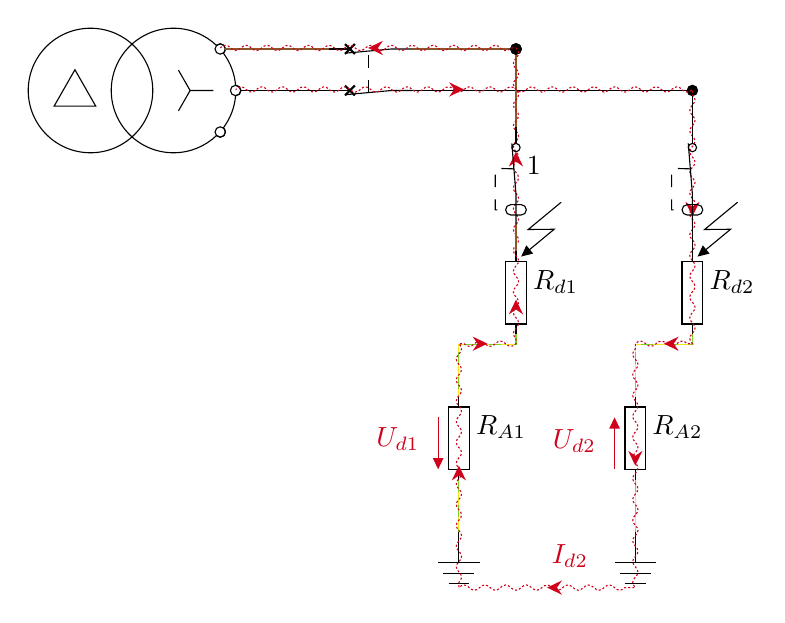
\begin{tikzpicture}[x=0.75pt,y=0.75pt,yscale=-1,xscale=1]
%uncomment if require: \path (0,314); %set diagram left start at 0, and has height of 314

%Straight Lines [id:da44771480202014247] 
\draw [color={rgb, 255:red, 0; green, 0; blue, 0 }  ,draw opacity=1 ]   (337.5,52.5) -- (337.5,35) ;
%Straight Lines [id:da5616221950341589] 
\draw    (202.5,35) -- (337.5,35) ;
%Straight Lines [id:da030139218122943512] 
\draw [color={rgb, 255:red, 139; green, 87; blue, 42 }  ,draw opacity=1 ]   (202.5,15) -- (252.5,15) ;
%Shape: Path Data [id:dp23022875443693058] 
\draw   (112.5,55) .. controls (112.5,56.38) and (111.38,57.5) .. (110,57.5) .. controls (109.29,57.5) and (108.65,57.2) .. (108.19,56.72) .. controls (102.81,61.85) and (95.52,65) .. (87.5,65) .. controls (70.93,65) and (57.5,51.57) .. (57.5,35) .. controls (57.5,18.43) and (70.93,5) .. (87.5,5) .. controls (95.52,5) and (102.81,8.15) .. (108.19,13.28) .. controls (108.65,12.8) and (109.29,12.5) .. (110,12.5) .. controls (111.38,12.5) and (112.5,13.62) .. (112.5,15) .. controls (112.5,15.82) and (112.11,16.54) .. (111.5,17) .. controls (114.8,21.39) and (116.92,26.71) .. (117.4,32.5) .. controls (117.43,32.5) and (117.47,32.5) .. (117.5,32.5) .. controls (118.88,32.5) and (120,33.62) .. (120,35) .. controls (120,36.38) and (118.88,37.5) .. (117.5,37.5) .. controls (117.47,37.5) and (117.43,37.5) .. (117.4,37.5) .. controls (116.92,43.29) and (114.8,48.61) .. (111.5,53) .. controls (112.11,53.46) and (112.5,54.18) .. (112.5,55) -- cycle ;
%Shape: Circle [id:dp1357901111827381] 
\draw   (17.5,35) .. controls (17.5,18.43) and (30.93,5) .. (47.5,5) .. controls (64.07,5) and (77.5,18.43) .. (77.5,35) .. controls (77.5,51.57) and (64.07,65) .. (47.5,65) .. controls (30.93,65) and (17.5,51.57) .. (17.5,35) -- cycle ;
%Shape: Triangle [id:dp7632621922673382] 
\draw   (40,25) -- (30,42.5) -- (50,42.5) -- cycle ;
%Shape: Star [id:dp9731649410229973] 
\draw   (106.75,35) -- (95.5,35) -- (89.88,44.81) -- (95.5,35) -- (89.88,25.19) -- (95.5,35) -- cycle ;
%Shape: Circle [id:dp31079836431690466] 
\draw   (107.5,15) .. controls (107.5,13.62) and (108.62,12.5) .. (110,12.5) .. controls (111.38,12.5) and (112.5,13.62) .. (112.5,15) .. controls (112.5,16.38) and (111.38,17.5) .. (110,17.5) .. controls (108.62,17.5) and (107.5,16.38) .. (107.5,15) -- cycle ;
%Shape: Circle [id:dp12266233820557082] 
\draw   (114.9,35) .. controls (114.9,33.62) and (116.02,32.5) .. (117.4,32.5) .. controls (118.78,32.5) and (119.9,33.62) .. (119.9,35) .. controls (119.9,36.38) and (118.78,37.5) .. (117.4,37.5) .. controls (116.02,37.5) and (114.9,36.38) .. (114.9,35) -- cycle ;
%Shape: Circle [id:dp5285901626538249] 
\draw   (107.5,55) .. controls (107.5,53.62) and (108.62,52.5) .. (110,52.5) .. controls (111.38,52.5) and (112.5,53.62) .. (112.5,55) .. controls (112.5,56.38) and (111.38,57.5) .. (110,57.5) .. controls (108.62,57.5) and (107.5,56.38) .. (107.5,55) -- cycle ;

%Straight Lines [id:da92188130951024] 
\draw [color={rgb, 255:red, 248; green, 231; blue, 28 }  ,draw opacity=1 ]   (225,222.5) -- (225,247.5) ;
%Straight Lines [id:da4292625671170487] 
\draw    (225,247.5) -- (225,262.5) ;
%Straight Lines [id:da06158937078168358] 
\draw    (215,262.5) -- (235,262.5) ;
%Straight Lines [id:da34789977188703036] 
\draw    (217.5,267.5) -- (232.5,267.5) ;
%Straight Lines [id:da1284483495628228] 
\draw    (220,272.5) -- (230,272.5) ;

%Straight Lines [id:da9082827551048067] 
\draw [color={rgb, 255:red, 126; green, 211; blue, 33 }  ,draw opacity=1 ] [dash pattern={on 4.5pt off 4.5pt}]  (225,222.5) -- (225,247.5) ;
%Straight Lines [id:da3209999402872329] 
\draw    (225,217.5) -- (225,222.5) ;
%Shape: Rectangle [id:dp2593386875607734] 
\draw   (230,187.5) -- (230,217.5) -- (220,217.5) -- (220,187.5) -- cycle ;
%Straight Lines [id:da740170600357607] 
\draw    (225,182.5) -- (225,187.5) ;

%Shape: Circle [id:dp8601483461254399] 
\draw  [fill={rgb, 255:red, 0; green, 0; blue, 0 }  ,fill opacity=1 ] (335,35) .. controls (335,33.62) and (336.12,32.5) .. (337.5,32.5) .. controls (338.88,32.5) and (340,33.62) .. (340,35) .. controls (340,36.38) and (338.88,37.5) .. (337.5,37.5) .. controls (336.12,37.5) and (335,36.38) .. (335,35) -- cycle ;
%Shape: Circle [id:dp12093020485396755] 
\draw  [fill={rgb, 255:red, 0; green, 0; blue, 0 }  ,fill opacity=1 ] (250,15) .. controls (250,13.62) and (251.12,12.5) .. (252.5,12.5) .. controls (253.88,12.5) and (255,13.62) .. (255,15) .. controls (255,16.38) and (253.88,17.5) .. (252.5,17.5) .. controls (251.12,17.5) and (250,16.38) .. (250,15) -- cycle ;
%Straight Lines [id:da2667129361258299] 
\draw [color={rgb, 255:red, 139; green, 87; blue, 42 }  ,draw opacity=1 ]   (112.5,15) -- (162.5,15) ;
%Straight Lines [id:da7247612407560878] 
\draw    (120,35) -- (162.5,35) ;
%Straight Lines [id:da9818089865990709] 
\draw    (310,217.5) -- (310,222.5) ;
%Shape: Rectangle [id:dp5739667555283554] 
\draw   (315,187.5) -- (315,217.5) -- (305,217.5) -- (305,187.5) -- cycle ;
%Straight Lines [id:da37673824938051304] 
\draw    (310,182.5) -- (310,187.5) ;

%Straight Lines [id:da9108771567706163] 
\draw [color={rgb, 255:red, 248; green, 231; blue, 28 }  ,draw opacity=1 ]   (310,222.5) -- (310,247.5) ;
%Straight Lines [id:da7506296134174059] 
\draw    (310,247.5) -- (310,262.5) ;
%Straight Lines [id:da8877376114904583] 
\draw    (300,262.5) -- (320,262.5) ;
%Straight Lines [id:da7805584248970565] 
\draw    (302.5,267.5) -- (317.5,267.5) ;
%Straight Lines [id:da4987046828919294] 
\draw    (305,272.5) -- (315,272.5) ;

%Straight Lines [id:da07069683992258613] 
\draw [color={rgb, 255:red, 126; green, 211; blue, 33 }  ,draw opacity=1 ] [dash pattern={on 4.5pt off 4.5pt}]  (310,222.5) -- (310,247.5) ;
%Shape: Boxed Line [id:dp017806634598713234] 
\draw    (274.27,88.83) -- (258.39,101.97) -- (270.89,101.86) -- (257.31,113.09) ;
\draw [shift={(255,115)}, rotate = 320.40999999999997] [fill={rgb, 255:red, 0; green, 0; blue, 0 }  ][line width=0.08]  [draw opacity=0] (5.36,-2.57) -- (0,0) -- (5.36,2.57) -- cycle    ;
%Shape: Boxed Line [id:dp8065003718686437] 
\draw    (359.27,88.83) -- (343.39,101.97) -- (355.89,101.86) -- (342.31,113.09) ;
\draw [shift={(340,115)}, rotate = 320.40999999999997] [fill={rgb, 255:red, 0; green, 0; blue, 0 }  ][line width=0.08]  [draw opacity=0] (5.36,-2.57) -- (0,0) -- (5.36,2.57) -- cycle    ;
%Straight Lines [id:da358454328833814] 
\draw    (170.5,37) -- (192.5,35) -- (202.5,35) ;
%Straight Lines [id:da868029205565597] 
\draw    (172.5,35) -- (162.5,35) ;
\draw [shift={(172.5,35)}, rotate = 225] [color={rgb, 255:red, 0; green, 0; blue, 0 }  ][line width=0.75]    (-3.35,0) -- (3.35,0)(0,3.35) -- (0,-3.35)   ;
%Straight Lines [id:da5656192330750602] 
\draw    (170.5,17) -- (192.5,15) -- (202.5,15) ;
%Straight Lines [id:da95863135682658] 
\draw  [dash pattern={on 4.5pt off 4.5pt}]  (181.5,36) -- (181.5,16) ;
%Straight Lines [id:da04894585565347964] 
\draw    (172.5,15) -- (162.5,15) ;
\draw [shift={(172.5,15)}, rotate = 225] [color={rgb, 255:red, 0; green, 0; blue, 0 }  ][line width=0.75]    (-3.35,0) -- (3.35,0)(0,3.35) -- (0,-3.35)   ;

%Straight Lines [id:da3293738134254155] 
\draw [color={rgb, 255:red, 139; green, 87; blue, 42 }  ,draw opacity=1 ]   (252.5,52.5) -- (252.5,15) ;
%Shape: Circle [id:dp8784736615935372] 
\draw  [fill={rgb, 255:red, 0; green, 0; blue, 0 }  ,fill opacity=1 ] (250,15) .. controls (250,13.62) and (251.12,12.5) .. (252.5,12.5) .. controls (253.88,12.5) and (255,13.62) .. (255,15) .. controls (255,16.38) and (253.88,17.5) .. (252.5,17.5) .. controls (251.12,17.5) and (250,16.38) .. (250,15) -- cycle ;
%Shape: Circle [id:dp11711924104585536] 
\draw  [fill={rgb, 255:red, 0; green, 0; blue, 0 }  ,fill opacity=1 ] (250,15) .. controls (250,13.62) and (251.12,12.5) .. (252.5,12.5) .. controls (253.88,12.5) and (255,13.62) .. (255,15) .. controls (255,16.38) and (253.88,17.5) .. (252.5,17.5) .. controls (251.12,17.5) and (250,16.38) .. (250,15) -- cycle ;
%Straight Lines [id:da08029921398538342] 
\draw    (252.5,147.5) -- (252.5,152.5) ;
%Shape: Rectangle [id:dp10461869500763998] 
\draw   (257.5,117.5) -- (257.5,147.5) -- (247.5,147.5) -- (247.5,117.5) -- cycle ;
%Straight Lines [id:da6711839663438437] 
\draw    (252.5,112.5) -- (252.5,117.5) ;

%Straight Lines [id:da306978016539733] 
\draw [color={rgb, 255:red, 208; green, 2; blue, 27 }  ,draw opacity=1 ]   (215,192.5) -- (215,214.5) ;
\draw [shift={(215,217.5)}, rotate = 270] [fill={rgb, 255:red, 208; green, 2; blue, 27 }  ,fill opacity=1 ][line width=0.08]  [draw opacity=0] (5.36,-2.57) -- (0,0) -- (5.36,2.57) -- cycle    ;
%Straight Lines [id:da9788903429329091] 
\draw [color={rgb, 255:red, 248; green, 231; blue, 28 }  ,draw opacity=1 ]   (252.5,152.5) -- (252.5,157.5) -- (225,157.5) -- (225,182.5) ;
%Straight Lines [id:da5746028122478745] 
\draw [color={rgb, 255:red, 126; green, 211; blue, 33 }  ,draw opacity=1 ] [dash pattern={on 4.5pt off 4.5pt}]  (252.5,152.5) -- (252.5,157.5) -- (225,157.5) -- (225,182.5) ;
%Straight Lines [id:da6637901588667133] 
\draw    (337.5,147.5) -- (337.5,152.5) ;
%Shape: Rectangle [id:dp33834418757589935] 
\draw   (342.5,117.5) -- (342.5,147.5) -- (332.5,147.5) -- (332.5,117.5) -- cycle ;
%Straight Lines [id:da4844708396236749] 
\draw    (337.5,112.5) -- (337.5,117.5) ;

%Straight Lines [id:da4767279022409927] 
\draw [color={rgb, 255:red, 208; green, 2; blue, 27 }  ,draw opacity=1 ]   (300,195.5) -- (300,217.5) ;
\draw [shift={(300,192.5)}, rotate = 90] [fill={rgb, 255:red, 208; green, 2; blue, 27 }  ,fill opacity=1 ][line width=0.08]  [draw opacity=0] (5.36,-2.57) -- (0,0) -- (5.36,2.57) -- cycle    ;
%Straight Lines [id:da015083238595793191] 
\draw [color={rgb, 255:red, 248; green, 231; blue, 28 }  ,draw opacity=1 ]   (337.5,152.5) -- (337.5,157.5) -- (310,157.5) -- (310,182.5) ;
%Straight Lines [id:da013265453939943717] 
\draw [color={rgb, 255:red, 126; green, 211; blue, 33 }  ,draw opacity=1 ] [dash pattern={on 4.5pt off 4.5pt}]  (337.5,152.5) -- (337.5,157.5) -- (310,157.5) -- (310,182.5) ;
%Straight Lines [id:da20369483289006973] 
\draw [color={rgb, 255:red, 208; green, 2; blue, 27 }  ,draw opacity=1 ] [dash pattern={on 0.75pt off 0.75pt}]  (110,14.5) .. controls (111.67,12.83) and (113.33,12.83) .. (115,14.5) .. controls (116.67,16.17) and (118.33,16.17) .. (120,14.5) .. controls (121.67,12.83) and (123.33,12.83) .. (125,14.5) .. controls (126.67,16.17) and (128.33,16.17) .. (130,14.5) .. controls (131.67,12.83) and (133.33,12.83) .. (135,14.5) .. controls (136.67,16.17) and (138.33,16.17) .. (140,14.5) .. controls (141.67,12.83) and (143.33,12.83) .. (145,14.5) .. controls (146.67,16.17) and (148.33,16.17) .. (150,14.5) .. controls (151.67,12.83) and (153.33,12.83) .. (155,14.5) .. controls (156.67,16.17) and (158.33,16.17) .. (160,14.5) .. controls (161.67,12.83) and (163.33,12.83) .. (165,14.5) .. controls (166.67,16.17) and (168.33,16.17) .. (170,14.5) .. controls (171.67,12.83) and (173.33,12.83) .. (175,14.5) .. controls (176.67,16.17) and (178.33,16.17) .. (180,14.5) .. controls (181.67,12.83) and (183.33,12.83) .. (185,14.5) .. controls (186.67,16.17) and (188.33,16.17) .. (190,14.5) .. controls (191.67,12.83) and (193.33,12.83) .. (195,14.5) .. controls (196.67,16.17) and (198.33,16.17) .. (200,14.5) .. controls (201.67,12.83) and (203.33,12.83) .. (205,14.5) .. controls (206.67,16.17) and (208.33,16.17) .. (210,14.5) .. controls (211.67,12.83) and (213.33,12.83) .. (215,14.5) .. controls (216.67,16.17) and (218.33,16.17) .. (220,14.5) .. controls (221.67,12.83) and (223.33,12.83) .. (225,14.5) .. controls (226.67,16.17) and (228.33,16.17) .. (230,14.5) .. controls (231.67,12.83) and (233.33,12.83) .. (235,14.5) .. controls (236.67,16.17) and (238.33,16.17) .. (240,14.5) .. controls (241.67,12.83) and (243.33,12.83) .. (245,14.5) .. controls (246.67,16.17) and (248.33,16.17) .. (250,14.5) -- (252.5,14.5) -- (252.5,14.5) .. controls (254.17,16.17) and (254.17,17.83) .. (252.5,19.5) .. controls (250.83,21.17) and (250.83,22.83) .. (252.5,24.5) .. controls (254.17,26.17) and (254.17,27.83) .. (252.5,29.5) .. controls (250.83,31.17) and (250.83,32.83) .. (252.5,34.5) .. controls (254.17,36.17) and (254.17,37.83) .. (252.5,39.5) .. controls (250.83,41.17) and (250.83,42.83) .. (252.5,44.5) .. controls (254.17,46.17) and (254.17,47.83) .. (252.5,49.5) .. controls (250.83,51.17) and (250.83,52.83) .. (252.5,54.5) .. controls (254.17,56.17) and (254.17,57.83) .. (252.5,59.5) .. controls (250.83,61.17) and (250.83,62.83) .. (252.5,64.5) .. controls (254.17,66.17) and (254.17,67.83) .. (252.5,69.5) .. controls (250.83,71.17) and (250.83,72.83) .. (252.5,74.5) .. controls (254.17,76.17) and (254.17,77.83) .. (252.5,79.5) .. controls (250.83,81.17) and (250.83,82.83) .. (252.5,84.5) .. controls (254.17,86.17) and (254.17,87.83) .. (252.5,89.5) .. controls (250.83,91.17) and (250.83,92.83) .. (252.5,94.5) .. controls (254.17,96.17) and (254.17,97.83) .. (252.5,99.5) .. controls (250.83,101.17) and (250.83,102.83) .. (252.5,104.5) .. controls (254.17,106.17) and (254.17,107.83) .. (252.5,109.5) .. controls (250.83,111.17) and (250.83,112.83) .. (252.5,114.5) -- (252.5,114.5) .. controls (254.17,116.17) and (254.17,117.83) .. (252.5,119.5) .. controls (250.83,121.17) and (250.83,122.83) .. (252.5,124.5) .. controls (254.17,126.17) and (254.17,127.83) .. (252.5,129.5) .. controls (250.83,131.17) and (250.83,132.83) .. (252.5,134.5) .. controls (254.17,136.17) and (254.17,137.83) .. (252.5,139.5) .. controls (250.83,141.17) and (250.83,142.83) .. (252.5,144.5) .. controls (254.17,146.17) and (254.17,147.83) .. (252.5,149.5) .. controls (250.83,151.17) and (250.83,152.83) .. (252.5,154.5) -- (252.5,157) -- (252.5,157) .. controls (250.83,158.67) and (249.17,158.67) .. (247.5,157) .. controls (245.83,155.33) and (244.17,155.33) .. (242.5,157) .. controls (240.83,158.67) and (239.17,158.67) .. (237.5,157) .. controls (235.83,155.33) and (234.17,155.33) .. (232.5,157) .. controls (230.83,158.67) and (229.17,158.67) .. (227.5,157) -- (225,157) -- (225,157) .. controls (226.67,158.67) and (226.67,160.33) .. (225,162) .. controls (223.33,163.67) and (223.33,165.33) .. (225,167) .. controls (226.67,168.67) and (226.67,170.33) .. (225,172) .. controls (223.33,173.67) and (223.33,175.33) .. (225,177) .. controls (226.67,178.67) and (226.67,180.33) .. (225,182) .. controls (223.33,183.67) and (223.33,185.33) .. (225,187) .. controls (226.67,188.67) and (226.67,190.33) .. (225,192) .. controls (223.33,193.67) and (223.33,195.33) .. (225,197) .. controls (226.67,198.67) and (226.67,200.33) .. (225,202) .. controls (223.33,203.67) and (223.33,205.33) .. (225,207) .. controls (226.67,208.67) and (226.67,210.33) .. (225,212) .. controls (223.33,213.67) and (223.33,215.33) .. (225,217) .. controls (226.67,218.67) and (226.67,220.33) .. (225,222) .. controls (223.33,223.67) and (223.33,225.33) .. (225,227) .. controls (226.67,228.67) and (226.67,230.33) .. (225,232) .. controls (223.33,233.67) and (223.33,235.33) .. (225,237) .. controls (226.67,238.67) and (226.67,240.33) .. (225,242) .. controls (223.33,243.67) and (223.33,245.33) .. (225,247) .. controls (226.67,248.67) and (226.67,250.33) .. (225,252) .. controls (223.33,253.67) and (223.33,255.33) .. (225,257) .. controls (226.67,258.67) and (226.67,260.33) .. (225,262) .. controls (223.33,263.67) and (223.33,265.33) .. (225,267) .. controls (226.67,268.67) and (226.67,270.33) .. (225,272) -- (225,274.5) -- (225,274.5) .. controls (226.67,272.83) and (228.33,272.83) .. (230,274.5) .. controls (231.67,276.17) and (233.33,276.17) .. (235,274.5) .. controls (236.67,272.83) and (238.33,272.83) .. (240,274.5) .. controls (241.67,276.17) and (243.33,276.17) .. (245,274.5) .. controls (246.67,272.83) and (248.33,272.83) .. (250,274.5) .. controls (251.67,276.17) and (253.33,276.17) .. (255,274.5) .. controls (256.67,272.83) and (258.33,272.83) .. (260,274.5) .. controls (261.67,276.17) and (263.33,276.17) .. (265,274.5) .. controls (266.67,272.83) and (268.33,272.83) .. (270,274.5) .. controls (271.67,276.17) and (273.33,276.17) .. (275,274.5) .. controls (276.67,272.83) and (278.33,272.83) .. (280,274.5) .. controls (281.67,276.17) and (283.33,276.17) .. (285,274.5) .. controls (286.67,272.83) and (288.33,272.83) .. (290,274.5) .. controls (291.67,276.17) and (293.33,276.17) .. (295,274.5) .. controls (296.67,272.83) and (298.33,272.83) .. (300,274.5) .. controls (301.67,276.17) and (303.33,276.17) .. (305,274.5) -- (310,274.5) -- (310,274.5) .. controls (308.33,272.83) and (308.33,271.17) .. (310,269.5) .. controls (311.67,267.83) and (311.67,266.17) .. (310,264.5) .. controls (308.33,262.83) and (308.33,261.17) .. (310,259.5) .. controls (311.67,257.83) and (311.67,256.17) .. (310,254.5) .. controls (308.33,252.83) and (308.33,251.17) .. (310,249.5) .. controls (311.67,247.83) and (311.67,246.17) .. (310,244.5) .. controls (308.33,242.83) and (308.33,241.17) .. (310,239.5) .. controls (311.67,237.83) and (311.67,236.17) .. (310,234.5) .. controls (308.33,232.83) and (308.33,231.17) .. (310,229.5) .. controls (311.67,227.83) and (311.67,226.17) .. (310,224.5) .. controls (308.33,222.83) and (308.33,221.17) .. (310,219.5) .. controls (311.67,217.83) and (311.67,216.17) .. (310,214.5) .. controls (308.33,212.83) and (308.33,211.17) .. (310,209.5) .. controls (311.67,207.83) and (311.67,206.17) .. (310,204.5) .. controls (308.33,202.83) and (308.33,201.17) .. (310,199.5) .. controls (311.67,197.83) and (311.67,196.17) .. (310,194.5) .. controls (308.33,192.83) and (308.33,191.17) .. (310,189.5) .. controls (311.67,187.83) and (311.67,186.17) .. (310,184.5) .. controls (308.33,182.83) and (308.33,181.17) .. (310,179.5) .. controls (311.67,177.83) and (311.67,176.17) .. (310,174.5) .. controls (308.33,172.83) and (308.33,171.17) .. (310,169.5) .. controls (311.67,167.83) and (311.67,166.17) .. (310,164.5) .. controls (308.33,162.83) and (308.33,161.17) .. (310,159.5) -- (310,157) -- (310,157) .. controls (311.67,155.33) and (313.33,155.33) .. (315,157) .. controls (316.67,158.67) and (318.33,158.67) .. (320,157) .. controls (321.67,155.33) and (323.33,155.33) .. (325,157) .. controls (326.67,158.67) and (328.33,158.67) .. (330,157) .. controls (331.67,155.33) and (333.33,155.33) .. (335,157) -- (337.5,157) -- (337.5,157) .. controls (335.83,155.33) and (335.83,153.67) .. (337.5,152) .. controls (339.17,150.33) and (339.17,148.67) .. (337.5,147) .. controls (335.83,145.33) and (335.83,143.67) .. (337.5,142) .. controls (339.17,140.33) and (339.17,138.67) .. (337.5,137) .. controls (335.83,135.33) and (335.83,133.67) .. (337.5,132) .. controls (339.17,130.33) and (339.17,128.67) .. (337.5,127) .. controls (335.83,125.33) and (335.83,123.67) .. (337.5,122) .. controls (339.17,120.33) and (339.17,118.67) .. (337.5,117) .. controls (335.83,115.33) and (335.83,113.67) .. (337.5,112) .. controls (339.17,110.33) and (339.17,108.67) .. (337.5,107) .. controls (335.83,105.33) and (335.83,103.67) .. (337.5,102) .. controls (339.17,100.33) and (339.17,98.67) .. (337.5,97) .. controls (335.83,95.33) and (335.83,93.67) .. (337.5,92) .. controls (339.17,90.33) and (339.17,88.67) .. (337.5,87) .. controls (335.83,85.33) and (335.83,83.67) .. (337.5,82) .. controls (339.17,80.33) and (339.17,78.67) .. (337.5,77) .. controls (335.83,75.33) and (335.83,73.67) .. (337.5,72) .. controls (339.17,70.33) and (339.17,68.67) .. (337.5,67) .. controls (335.83,65.33) and (335.83,63.67) .. (337.5,62) .. controls (339.17,60.33) and (339.17,58.67) .. (337.5,57) .. controls (335.83,55.33) and (335.83,53.67) .. (337.5,52) .. controls (339.17,50.33) and (339.17,48.67) .. (337.5,47) .. controls (335.83,45.33) and (335.83,43.67) .. (337.5,42) .. controls (339.17,40.33) and (339.17,38.67) .. (337.5,37) -- (337.5,34.5) -- (337.5,34.5) .. controls (335.83,36.17) and (334.17,36.17) .. (332.5,34.5) .. controls (330.83,32.83) and (329.17,32.83) .. (327.5,34.5) .. controls (325.83,36.17) and (324.17,36.17) .. (322.5,34.5) .. controls (320.83,32.83) and (319.17,32.83) .. (317.5,34.5) .. controls (315.83,36.17) and (314.17,36.17) .. (312.5,34.5) .. controls (310.83,32.83) and (309.17,32.83) .. (307.5,34.5) .. controls (305.83,36.17) and (304.17,36.17) .. (302.5,34.5) .. controls (300.83,32.83) and (299.17,32.83) .. (297.5,34.5) .. controls (295.83,36.17) and (294.17,36.17) .. (292.5,34.5) .. controls (290.83,32.83) and (289.17,32.83) .. (287.5,34.5) .. controls (285.83,36.17) and (284.17,36.17) .. (282.5,34.5) .. controls (280.83,32.83) and (279.17,32.83) .. (277.5,34.5) .. controls (275.83,36.17) and (274.17,36.17) .. (272.5,34.5) .. controls (270.83,32.83) and (269.17,32.83) .. (267.5,34.5) .. controls (265.83,36.17) and (264.17,36.17) .. (262.5,34.5) .. controls (260.83,32.83) and (259.17,32.83) .. (257.5,34.5) .. controls (255.83,36.17) and (254.17,36.17) .. (252.5,34.5) .. controls (250.83,32.83) and (249.17,32.83) .. (247.5,34.5) .. controls (245.83,36.17) and (244.17,36.17) .. (242.5,34.5) .. controls (240.83,32.83) and (239.17,32.83) .. (237.5,34.5) .. controls (235.83,36.17) and (234.17,36.17) .. (232.5,34.5) .. controls (230.83,32.83) and (229.17,32.83) .. (227.5,34.5) .. controls (225.83,36.17) and (224.17,36.17) .. (222.5,34.5) .. controls (220.83,32.83) and (219.17,32.83) .. (217.5,34.5) .. controls (215.83,36.17) and (214.17,36.17) .. (212.5,34.5) .. controls (210.83,32.83) and (209.17,32.83) .. (207.5,34.5) .. controls (205.83,36.17) and (204.17,36.17) .. (202.5,34.5) .. controls (200.83,32.83) and (199.17,32.83) .. (197.5,34.5) .. controls (195.83,36.17) and (194.17,36.17) .. (192.5,34.5) .. controls (190.83,32.83) and (189.17,32.83) .. (187.5,34.5) .. controls (185.83,36.17) and (184.17,36.17) .. (182.5,34.5) .. controls (180.83,32.83) and (179.17,32.83) .. (177.5,34.5) .. controls (175.83,36.17) and (174.17,36.17) .. (172.5,34.5) .. controls (170.83,32.83) and (169.17,32.83) .. (167.5,34.5) .. controls (165.83,36.17) and (164.17,36.17) .. (162.5,34.5) .. controls (160.83,32.83) and (159.17,32.83) .. (157.5,34.5) .. controls (155.83,36.17) and (154.17,36.17) .. (152.5,34.5) .. controls (150.83,32.83) and (149.17,32.83) .. (147.5,34.5) .. controls (145.83,36.17) and (144.17,36.17) .. (142.5,34.5) .. controls (140.83,32.83) and (139.17,32.83) .. (137.5,34.5) .. controls (135.83,36.17) and (134.17,36.17) .. (132.5,34.5) .. controls (130.83,32.83) and (129.17,32.83) .. (127.5,34.5) .. controls (125.83,36.17) and (124.17,36.17) .. (122.5,34.5) .. controls (120.83,32.83) and (119.17,32.83) .. (117.5,34.5) -- (117.4,34.5) -- (117.4,34.5) ;
\draw [shift={(181.25,14.5)}, rotate = 0] [fill={rgb, 255:red, 208; green, 2; blue, 27 }  ,fill opacity=1 ][line width=0.08]  [draw opacity=0] (7.14,-3.43) -- (0,0) -- (7.14,3.43) -- (4.74,0) -- cycle    ;
\draw [shift={(252.5,64.5)}, rotate = 90] [fill={rgb, 255:red, 208; green, 2; blue, 27 }  ,fill opacity=1 ][line width=0.08]  [draw opacity=0] (7.14,-3.43) -- (0,0) -- (7.14,3.43) -- (4.74,0) -- cycle    ;
\draw [shift={(252.5,135.75)}, rotate = 90] [fill={rgb, 255:red, 208; green, 2; blue, 27 }  ,fill opacity=1 ][line width=0.08]  [draw opacity=0] (7.14,-3.43) -- (0,0) -- (7.14,3.43) -- (4.74,0) -- cycle    ;
\draw [shift={(238.75,157)}, rotate = 180] [fill={rgb, 255:red, 208; green, 2; blue, 27 }  ,fill opacity=1 ][line width=0.08]  [draw opacity=0] (7.14,-3.43) -- (0,0) -- (7.14,3.43) -- (4.74,0) -- cycle    ;
\draw [shift={(225,215.75)}, rotate = 90] [fill={rgb, 255:red, 208; green, 2; blue, 27 }  ,fill opacity=1 ][line width=0.08]  [draw opacity=0] (7.14,-3.43) -- (0,0) -- (7.14,3.43) -- (4.74,0) -- cycle    ;
\draw [shift={(267.5,274.5)}, rotate = 0] [fill={rgb, 255:red, 208; green, 2; blue, 27 }  ,fill opacity=1 ][line width=0.08]  [draw opacity=0] (7.14,-3.43) -- (0,0) -- (7.14,3.43) -- (4.74,0) -- cycle    ;
\draw [shift={(310,215.75)}, rotate = 270] [fill={rgb, 255:red, 208; green, 2; blue, 27 }  ,fill opacity=1 ][line width=0.08]  [draw opacity=0] (7.14,-3.43) -- (0,0) -- (7.14,3.43) -- (4.74,0) -- cycle    ;
\draw [shift={(323.75,157)}, rotate = 0] [fill={rgb, 255:red, 208; green, 2; blue, 27 }  ,fill opacity=1 ][line width=0.08]  [draw opacity=0] (7.14,-3.43) -- (0,0) -- (7.14,3.43) -- (4.74,0) -- cycle    ;
\draw [shift={(337.5,95.75)}, rotate = 270] [fill={rgb, 255:red, 208; green, 2; blue, 27 }  ,fill opacity=1 ][line width=0.08]  [draw opacity=0] (7.14,-3.43) -- (0,0) -- (7.14,3.43) -- (4.74,0) -- cycle    ;
\draw [shift={(227.45,34.5)}, rotate = 180] [fill={rgb, 255:red, 208; green, 2; blue, 27 }  ,fill opacity=1 ][line width=0.08]  [draw opacity=0] (7.14,-3.43) -- (0,0) -- (7.14,3.43) -- (4.74,0) -- cycle    ;
%Shape: Circle [id:dp6688360070263407] 
\draw   (254.5,62.5) .. controls (254.5,61.4) and (253.6,60.5) .. (252.5,60.5) .. controls (251.4,60.5) and (250.5,61.4) .. (250.5,62.5) .. controls (250.5,63.6) and (251.4,64.5) .. (252.5,64.5) .. controls (253.6,64.5) and (254.5,63.6) .. (254.5,62.5) -- cycle ;
%Straight Lines [id:da023498503244457125] 
\draw    (252.5,60.5) -- (252.5,52.5) ;
%Rounded Rect [id:dp30279070557566734] 
\draw   (247.5,92.5) .. controls (247.5,91.12) and (248.62,90) .. (250,90) -- (255,90) .. controls (256.38,90) and (257.5,91.12) .. (257.5,92.5) -- (257.5,92.5) .. controls (257.5,93.88) and (256.38,95) .. (255,95) -- (250,95) .. controls (248.62,95) and (247.5,93.88) .. (247.5,92.5) -- cycle ;
%Straight Lines [id:da16468651371944532] 
\draw  [dash pattern={on 4.5pt off 4.5pt}]  (251.5,72.75) -- (242.5,72.5) -- (242.5,92.5) -- (247.5,92.5) ;
%Straight Lines [id:da8036936912023739] 
\draw    (250.5,60.5) -- (252.5,85) -- (252.5,100) ;

%Shape: Circle [id:dp7937625551850244] 
\draw   (339.5,62.5) .. controls (339.5,61.4) and (338.6,60.5) .. (337.5,60.5) .. controls (336.4,60.5) and (335.5,61.4) .. (335.5,62.5) .. controls (335.5,63.6) and (336.4,64.5) .. (337.5,64.5) .. controls (338.6,64.5) and (339.5,63.6) .. (339.5,62.5) -- cycle ;
%Straight Lines [id:da5242903170497772] 
\draw    (337.5,60.5) -- (337.5,52.5) ;
%Rounded Rect [id:dp6818768532487535] 
\draw   (332.5,92.5) .. controls (332.5,91.12) and (333.62,90) .. (335,90) -- (340,90) .. controls (341.38,90) and (342.5,91.12) .. (342.5,92.5) -- (342.5,92.5) .. controls (342.5,93.88) and (341.38,95) .. (340,95) -- (335,95) .. controls (333.62,95) and (332.5,93.88) .. (332.5,92.5) -- cycle ;
%Straight Lines [id:da0851882978686429] 
\draw  [dash pattern={on 4.5pt off 4.5pt}]  (336.5,72.75) -- (327.5,72.5) -- (327.5,92.5) -- (332.5,92.5) ;
%Straight Lines [id:da2719116658142192] 
\draw    (335.5,60.5) -- (337.5,85) -- (337.5,100) ;

%Straight Lines [id:da23106759511180686] 
\draw [color={rgb, 255:red, 139; green, 87; blue, 42 }  ,draw opacity=1 ]   (252.5,112.5) -- (252.5,100) ;
%Straight Lines [id:da04628877500711526] 
\draw [color={rgb, 255:red, 0; green, 0; blue, 0 }  ,draw opacity=1 ]   (337.5,112.5) -- (337.5,100) ;


% Text Node
\draw (232,190.5) node [anchor=north west][inner sep=0.75pt]   [align=left] {$R_{A1}$};
% Text Node
\draw (317,190.5) node [anchor=north west][inner sep=0.75pt]   [align=left] {$R_{A2}$};
% Text Node
\draw (268.5,252.5) node [anchor=north west][inner sep=0.75pt]  [color={rgb, 255:red, 208; green, 2; blue, 27 }  ,opacity=1 ] [align=left] {$I_{d2}$};
% Text Node
\draw (184,196) node [anchor=north west][inner sep=0.75pt]  [color={rgb, 255:red, 208; green, 2; blue, 27 }  ,opacity=1 ] [align=left] {$U_{d1}$};
% Text Node
\draw (259.5,120.5) node [anchor=north west][inner sep=0.75pt]   [align=left] {$R_{d1}$};
% Text Node
\draw (269,197) node [anchor=north west][inner sep=0.75pt]  [color={rgb, 255:red, 208; green, 2; blue, 27 }  ,opacity=1 ] [align=left] {$U_{d2}$};
% Text Node
\draw (344.5,120.5) node [anchor=north west][inner sep=0.75pt]   [align=left] {$R_{d2}$};
% Text Node
\draw (256.5,65.5) node [anchor=north west][inner sep=0.75pt]   [align=left] {\Circled{1}};

\end{tikzpicture}


\end{figure}

%\end{document}


L'intensité de courant $I_{d2}$ vaut alors :
\begin{formule}[Courant du deuxième défaut $I_{d2}$ en schéma Isolé-Individuel]
\begin{align*}
		I_{d2} &= \frac{U}{R_{d1}+R_{A1}+R_{A2}+R_{A2}} \\
\end{align*}
\end{formule}

\begin{textvariables}
U								& tension nominale composée				& volt			& \volt					& 	Différence de potentiel entre deux conducteurs actifs (à préciser s'il s'agit du conducteur neutre)	\\
R_{d1}						& résistance											& ohm			& \ohm					& 	Résistance de défaut 	d'isolement de l'appareil 1\\
R_{A1}						& résistance											& ohm			& \ohm					& 	Résistance de la prise de terre de l'appareil 1 	\\
R_{A2}						& résistance											& ohm			& \ohm					& 	Résistance de la prise de terre de l'appareil 2 	\\
R_{d2}						& résistance											& ohm			& \ohm					& 	Résistance de défaut 	d'isolement de l'appareil 1\\
\end{textvariables}

Le courant de défaut $I_{d1}$ fera alors apparaître une \emph{tension de défaut} $U_{d1}$ entre la masse métallique de l'appareil 1 et la terre. Cette tension, limitée par l'impédance de fuite, sera très largement inférieure à  $U_L$ et ne sera donc pas dangereuse. La situation sera similaire avec un schéma Impédant-Individuel $Z_N$, ou l'impédance de limitation limitera également le courant de défaut :

\begin{formule}[Tension de défaut $U_{d1}$ en schéma Isolé-Individuel]
\begin{align*}
		U_{d1} &= R_{A1} \times I_{d2} \\
					&<	U_L
\end{align*}
\end{formule}

\begin{textvariables}
R_{A1}						& résistance											& ohm			& \ohm					& 	Résistance de la prise de terre de l'appareil 1 	\\
I_{d2}						& intensité												& ampère		& \ampere				& 	Courant de défaut de l'appareil 2 \\
U_{L}						& tension							& volt			& \volt										& 	Tension de sécurité du local avec :
\begin{description}[nosep, leftmargin=*]
\item[Local sec :] $U_{L}=\SI{50}{\volt}$
\item[Local humide :] $U_{L}=\SI{25}{\volt}$
\end{description} \\
\end{textvariables}

Le cas est similaire à ceux rencontrés en schéma TT, on procèdera de la même manière en protégeant chaque groupe de masses par un DDR au calibre adapté \Circled{1}. Il est donc nécessaire de limiter $U_{d1}$ à la valeur suivante (voir \superref{form:resistance_prise_terre}) :

\begin{formule}[Calibre du DDR $I_{\Delta n}$]
\begin{align}
		I_{\Delta n} &< \frac{U_{L}}{R_{A1}}
\end{align}
\end{formule}

\begin{textvariables}
R_{A1}						& résistance											& ohm			& \ohm					& 	Résistance de la prise de terre de l'appareil 1 	\\
U_{L}						& tension							& volt			& \volt					& 	Tension de sécurité du local avec :
\begin{description}[nosep, leftmargin=*]
\item[Local sec :] $U_{L}=\SI{50}{\volt}$
\item[Local humide :] $U_{L}=\SI{25}{\volt}$
\end{description} \\
R_{A1}						& résistance											& ohm			& \ohm					& 	Résistance de la prise de terre de l'appareil 1 	\\
\end{textvariables}

L'usage de DDR implique de tenir du courant du premier défaut d'isolement $I_{d1}$ afin que la protection ne coupe pas le circuit dès le premier défaut :

\begin{table}[h]
\caption{Correspondance entre la capacité de fuite et le courant de premier défaut d'isolement}
\begin{tabular}{cc}
\toprule
\thead{Capacité de fuite (\si{\micro\farad})} 	&	\thead{Courant de premier défaut (\si{\ampere})} \\
\midrule
1		&	0,07 \\
5		& 0,36 \\
30		& 2,17 \\
\bottomrule
\end{tabular}
\end{table}

\begin{exemple}[Tension de défaut $U_{d1}$ en schéma Isolé-Individuel au deuxième défaut]
Si on considère que le transformateur est un transformateur $\SI{20}{\kilo\volt}/\SI{400}{\volt}$, que $R_{A1}=R_{A2}=\SI{40}{\ohm}$ et que $R_{d1} =R_{d1}= \SI{2}{\ohm}$, on peut déduire que le courant de défaut $I_{d2}$ vaut :
\begin{align*}
		I_{d2} &= \frac{U}{R_{d1}+R_{A1}+R_{A2}+R_{A2}} \\
					&=\frac{400}{2+40+40+2} \\
				&= \SI{4,76}{\ampere} \\
\end{align*}
Si une personne touche à la masse du récepteur 1, elle sera soumise à une tension de défaut $U_{d1}$ :
\begin{align*}
		U_{d1} &= R_{A1} \times I_{d2} \\
				&=40 \times 4,76 \\
				&= \SI{190,4}{\volt}
\end{align*}
La tension de défaut $U_{d1}$ est dangereuse quelle que soit la tension limite choisie :
\begin{itemize}
\item coupure la plus rapide possible\,;
\item protection des personnes.
\end{itemize}
~\\
\begin{minipage}[t]{0.5\linewidth}
Dans le cas d'un local sec :
\begin{align*}
	I_{\Delta n} 	&< \frac{U_{L}}{R_{A1}} \\
						&< \frac{50}{40} \\
						&< \SI{1,25}{\ampere}
\end{align*}
\end{minipage}
\hfill
\begin{minipage}[t]{0.5\linewidth}
Dans le cas d'un local humide :
\begin{align*}
	I_{\Delta n} 	&< \frac{U_{L}}{R_{A1}} \\
						&< \frac{25}{40} \\
						&< \SI{0,625}{\ampere}
\end{align*}
\end{minipage}
~\\
D'après le tableau situé en \superref{tab:temps_coupure_DDR}, le DDR protégeant la carcasse de l'appareil 1 doit présenter un temps de coupure de moins de \SI{200}{\milli\second} avec une tension de défaut $U_d$ de \SI{190,4}{\volt} :

\begin{table}[h]
\begin{tabularx}{\linewidth}{X cccccccc}
\toprule
Tension nominale		& \multicolumn{2}{c}{$\SI{50}{\volt}<U_0\leq\SI{120}{\volt}$} 	& \multicolumn{2}{c}{$\SI{120}{\volt}<U_0\leq\SI{230}{\volt}$} & \multicolumn{2}{c}{$\SI{230}{\volt}<U_0\leq\SI{400}{\volt}$}		& \multicolumn{2}{c}{$U_0>\SI{400}{\volt}$}\\
\midrule
Type de courant		& alternatif	& continu	& alternatif	& continu	& alternatif	& continu	& alternatif	& continu \\
\addlinespace
Schéma TN/IT	& \SI{0,8}{\second}	&	\SI{5}{\second}	&	\SI{0,4}{\second}	&	\SI{5}{\second}	&	\SI{0,2}{\second}	&	\SI{0,4}{\second}	&	\SI{0,1}{\second}	&	\SI{0,1}{\second} \\	
\addlinespace
Schéma TT	& \SI{0,3}{\second}	&	\SI{5}{\second}	&	\cellcolor{green}\SI{0,2}{\second}	&	\SI{0,4}{\second}	&	\SI{0,07}{\second}	&	\SI{0,2}{\second}	&	\SI{0,04}{\second}	&	\SI{0,1}{\second} \\	
\bottomrule
\end{tabularx}
\end{table}
\end{exemple}

\subsection{Neutre isolé et masses interconnectées et mise à la terre}

Les situations saines et au premier défaut d'isolement d'une installation en schéma IT avec les masses conductrices interconnectées et reliés en un seul point seront similaires au schéma IT avec les masses mise à la terre individuellement. Au deuxième défaut d'isolement, la situation sera différente, la prise en charge du défaut va s'apparenter à celle qu'on rencontre en schéma TN avec l'apparition d'un court-circuit.

 \begin{figure}[H]
\caption{Installation Isolé-Interconnectée}
\begin{subfigure}[t]{0.49\linewidth}
%--------------------------------------
%ELECTROTECHNIQUE - SCHEMA DE LIAISON A LA TERRE
%--------------------------------------

%utiliser les environnement \begin{comment} \end{comment} pour mettre en commentaire le préambule une fois la programmation appelée dans le document maître (!ne pas oublier de mettre en commentaire \end{document}!)

\begin{comment}

\documentclass[a4paper, 11pt, twoside, fleqn]{memoir}

\usepackage{AOCDTF}

\marqueurchapitre
\decoupagechapitre{1} %juste pour éviter les erreurs lors de la compilation des sous-programmations (passera en commentaire)

%lien d'édition des figures Tikz sur le site mathcha.io (rajouter le lien d'une modification effectuée sur la figure tikz avec le nom du modificateur car il n'y a qu'un lien par compte)

%lien mathcha Bruno Douchy : https://www.mathcha.io/editor/DXXG1FgjiNJCe0yo2ZTqzEeM8hlg57ygtvk5Mpy

%--------------------------------------
%corps du document
%--------------------------------------

\begin{document} %corps du document
	\openleft %début de chapitre à gauche

\end{comment}

% Pattern Info
 
\tikzset{
pattern size/.store in=\mcSize, 
pattern size = 5pt,
pattern thickness/.store in=\mcThickness, 
pattern thickness = 0.3pt,
pattern radius/.store in=\mcRadius, 
pattern radius = 1pt}
\makeatletter
\pgfutil@ifundefined{pgf@pattern@name@_onpxm15pp}{
\pgfdeclarepatternformonly[\mcThickness,\mcSize]{_onpxm15pp}
{\pgfqpoint{0pt}{0pt}}
{\pgfpoint{\mcSize+\mcThickness}{\mcSize+\mcThickness}}
{\pgfpoint{\mcSize}{\mcSize}}
{
\pgfsetcolor{\tikz@pattern@color}
\pgfsetlinewidth{\mcThickness}
\pgfpathmoveto{\pgfqpoint{0pt}{0pt}}
\pgfpathlineto{\pgfpoint{\mcSize+\mcThickness}{\mcSize+\mcThickness}}
\pgfusepath{stroke}
}}
\makeatother
\tikzset{every picture/.style={line width=0.5pt}} %set default line width to 0.75pt        

\begin{tikzpicture}[x=0.75pt,y=0.75pt,yscale=-0.6,xscale=0.6]
%uncomment if require: \path (0,293); %set diagram left start at 0, and has height of 293

%Shape: Rectangle [id:dp06629411116627981] 
\draw  [dash pattern={on 2.25pt off 2.25pt on 1pt off 2.25pt}] (242.5,115) -- (302.5,115) -- (302.5,145) -- (242.5,145) -- cycle ;
%Shape: Rectangle [id:dp5496339182307807] 
\draw  [dash pattern={on 2.25pt off 2.25pt on 1pt off 2.25pt}] (327.5,115) -- (387.5,115) -- (387.5,145) -- (327.5,145) -- cycle ;
%Shape: Rectangle [id:dp30094494963346674] 
\draw  [dash pattern={on 2.25pt off 2.25pt on 1pt off 2.25pt}] (412.5,115) -- (472.5,115) -- (472.5,145) -- (412.5,145) -- cycle ;
%Straight Lines [id:da7855603359005625] 
\draw [color={rgb, 255:red, 74; green, 144; blue, 226 }  ,draw opacity=1 ]   (202.5,75.5) -- (462.5,75) ;
%Straight Lines [id:da3845932965061506] 
\draw [color={rgb, 255:red, 74; green, 144; blue, 226 }  ,draw opacity=1 ]   (90,75) -- (162.5,75) ;
%Straight Lines [id:da5834167633542386] 
\draw [color={rgb, 255:red, 248; green, 231; blue, 28 }  ,draw opacity=1 ]   (87.5,75) -- (27.5,75) -- (27.5,182.5) ;
%Straight Lines [id:da9429513177603445] 
\draw [color={rgb, 255:red, 248; green, 231; blue, 28 }  ,draw opacity=1 ]   (95.5,35) -- (87.5,75) -- (87.5,107.5) ;
%Straight Lines [id:da7600472701317061] 
\draw [color={rgb, 255:red, 126; green, 211; blue, 33 }  ,draw opacity=1 ] [dash pattern={on 2.25pt off 2.25pt}]  (95.5,35) -- (87.5,75) -- (87.5,107.5) ;
%Straight Lines [id:da6079599273540643] 
\draw [color={rgb, 255:red, 248; green, 231; blue, 28 }  ,draw opacity=1 ]   (240,135) -- (225,135) -- (225,182.5) ;
%Straight Lines [id:da8706050361736538] 
\draw    (202.5,35) -- (463.75,35) ;
%Straight Lines [id:da5697476802363065] 
\draw [color={rgb, 255:red, 139; green, 87; blue, 42 }  ,draw opacity=1 ]   (202.5,15) -- (462.5,15) ;
%Straight Lines [id:da9735954426571896] 
\draw [color={rgb, 255:red, 155; green, 155; blue, 155 }  ,draw opacity=1 ]   (202.5,55) -- (462.5,55) ;
%Shape: Path Data [id:dp36735613758138397] 
\draw   (112.5,55) .. controls (112.5,56.38) and (111.38,57.5) .. (110,57.5) .. controls (109.29,57.5) and (108.65,57.2) .. (108.19,56.72) .. controls (102.81,61.85) and (95.52,65) .. (87.5,65) .. controls (70.93,65) and (57.5,51.57) .. (57.5,35) .. controls (57.5,18.43) and (70.93,5) .. (87.5,5) .. controls (95.52,5) and (102.81,8.15) .. (108.19,13.28) .. controls (108.65,12.8) and (109.29,12.5) .. (110,12.5) .. controls (111.38,12.5) and (112.5,13.62) .. (112.5,15) .. controls (112.5,15.82) and (112.11,16.54) .. (111.5,17) .. controls (114.8,21.39) and (116.92,26.71) .. (117.4,32.5) .. controls (117.43,32.5) and (117.47,32.5) .. (117.5,32.5) .. controls (118.88,32.5) and (120,33.62) .. (120,35) .. controls (120,36.38) and (118.88,37.5) .. (117.5,37.5) .. controls (117.47,37.5) and (117.43,37.5) .. (117.4,37.5) .. controls (116.92,43.29) and (114.8,48.61) .. (111.5,53) .. controls (112.11,53.46) and (112.5,54.18) .. (112.5,55) -- cycle ;
%Shape: Circle [id:dp23421524241037028] 
\draw   (17.5,35) .. controls (17.5,18.43) and (30.93,5) .. (47.5,5) .. controls (64.07,5) and (77.5,18.43) .. (77.5,35) .. controls (77.5,51.57) and (64.07,65) .. (47.5,65) .. controls (30.93,65) and (17.5,51.57) .. (17.5,35) -- cycle ;
%Shape: Triangle [id:dp48236106138172463] 
\draw   (40,25) -- (30,42.5) -- (50,42.5) -- cycle ;
%Shape: Star [id:dp8682414008103251] 
\draw   (106.75,35) -- (95.5,35) -- (89.88,44.81) -- (95.5,35) -- (89.88,25.19) -- (95.5,35) -- cycle ;
%Shape: Circle [id:dp74403652528276] 
\draw   (107.5,15) .. controls (107.5,13.62) and (108.62,12.5) .. (110,12.5) .. controls (111.38,12.5) and (112.5,13.62) .. (112.5,15) .. controls (112.5,16.38) and (111.38,17.5) .. (110,17.5) .. controls (108.62,17.5) and (107.5,16.38) .. (107.5,15) -- cycle ;
%Shape: Circle [id:dp12230623178485356] 
\draw   (114.9,35) .. controls (114.9,33.62) and (116.02,32.5) .. (117.4,32.5) .. controls (118.78,32.5) and (119.9,33.62) .. (119.9,35) .. controls (119.9,36.38) and (118.78,37.5) .. (117.4,37.5) .. controls (116.02,37.5) and (114.9,36.38) .. (114.9,35) -- cycle ;
%Shape: Circle [id:dp8868519788786934] 
\draw   (107.5,55) .. controls (107.5,53.62) and (108.62,52.5) .. (110,52.5) .. controls (111.38,52.5) and (112.5,53.62) .. (112.5,55) .. controls (112.5,56.38) and (111.38,57.5) .. (110,57.5) .. controls (108.62,57.5) and (107.5,56.38) .. (107.5,55) -- cycle ;

%Straight Lines [id:da4565704928737364] 
\draw [color={rgb, 255:red, 74; green, 144; blue, 226 }  ,draw opacity=1 ]   (292.5,127.5) -- (292.5,77.5) ;
%Straight Lines [id:da08957212555201388] 
\draw [color={rgb, 255:red, 139; green, 87; blue, 42 }  ,draw opacity=1 ]   (252.5,127.5) -- (252.5,17.5) ;
%Straight Lines [id:da7418535885736515] 
\draw [color={rgb, 255:red, 139; green, 87; blue, 42 }  ,draw opacity=1 ]   (252.5,130) -- (252.5,117.5) ;
%Straight Lines [id:da8720965180296373] 
\draw [color={rgb, 255:red, 74; green, 144; blue, 226 }  ,draw opacity=1 ]   (292.5,130.5) -- (292.5,117.5) ;
%Straight Lines [id:da938936503356733] 
\draw    (17.5,232.5) -- (460,232.5) ;
%Shape: Rectangle [id:dp7311273665746781] 
\draw  [draw opacity=0][pattern=_onpxm15pp,pattern size=6pt,pattern thickness=0.75pt,pattern radius=0pt, pattern color={rgb, 255:red, 0; green, 0; blue, 0}][line width=0.75]  (17.5,232.5) -- (460,232.5) -- (460,247.5) -- (17.5,247.5) -- cycle ;
%Straight Lines [id:da8141513336558377] 
\draw [color={rgb, 255:red, 126; green, 211; blue, 33 }  ,draw opacity=1 ] [dash pattern={on 2.25pt off 2.25pt}]  (240,135) -- (225,135) -- (225,182.5) ;
%Straight Lines [id:da29843762221307424] 
\draw [color={rgb, 255:red, 248; green, 231; blue, 28 }  ,draw opacity=1 ]   (225,222.5) -- (225,247.5) ;
%Straight Lines [id:da11084730612327653] 
\draw    (225,247.5) -- (225,262.5) ;
%Straight Lines [id:da28813972378566177] 
\draw    (215,262.5) -- (235,262.5) ;
%Straight Lines [id:da12034369105457465] 
\draw    (217.5,267.5) -- (232.5,267.5) ;
%Straight Lines [id:da6195695090232725] 
\draw    (220,272.5) -- (230,272.5) ;

%Straight Lines [id:da7010427793052417] 
\draw [color={rgb, 255:red, 126; green, 211; blue, 33 }  ,draw opacity=1 ] [dash pattern={on 2.25pt off 2.25pt}]  (225,222.5) -- (225,247.5) ;
%Straight Lines [id:da6639632595865842] 
\draw    (287.5,130) -- (292.5,130) ;
%Shape: Rectangle [id:dp48750397418832736] 
\draw   (257.5,125) -- (287.5,125) -- (287.5,135) -- (257.5,135) -- cycle ;
%Straight Lines [id:da3091869002192609] 
\draw    (252.5,130) -- (257.5,130) ;

%Straight Lines [id:da46843421066318236] 
\draw    (225,217.5) -- (225,222.5) ;
%Shape: Rectangle [id:dp8288861680700458] 
\draw   (230,187.5) -- (230,217.5) -- (220,217.5) -- (220,187.5) -- cycle ;
%Straight Lines [id:da39538233114745247] 
\draw    (225,182.5) -- (225,187.5) ;

%Straight Lines [id:da03908999537683522] 
\draw [color={rgb, 255:red, 74; green, 144; blue, 226 }  ,draw opacity=1 ]   (377.5,127.5) -- (377.5,77.5) ;
%Straight Lines [id:da014322617412467653] 
\draw [color={rgb, 255:red, 0; green, 0; blue, 0 }  ,draw opacity=1 ]   (337.5,127.5) -- (337.5,35) ;
%Straight Lines [id:da37678293812005714] 
\draw [color={rgb, 255:red, 74; green, 144; blue, 226 }  ,draw opacity=1 ]   (377.5,130.5) -- (377.5,117.5) ;
%Straight Lines [id:da9817945211819089] 
\draw    (372.5,130) -- (377.5,130) ;
%Shape: Rectangle [id:dp3965217784422401] 
\draw   (342.5,125) -- (372.5,125) -- (372.5,135) -- (342.5,135) -- cycle ;
%Straight Lines [id:da03329133725543032] 
\draw    (337.5,130) -- (342.5,130) ;

%Straight Lines [id:da8796176191529531] 
\draw [color={rgb, 255:red, 74; green, 144; blue, 226 }  ,draw opacity=1 ]   (462.5,127.5) -- (462.5,77.5) ;
%Straight Lines [id:da6222130388950533] 
\draw [color={rgb, 255:red, 155; green, 155; blue, 155 }  ,draw opacity=1 ]   (422.5,127.5) -- (422.5,55) ;
%Straight Lines [id:da25889379629104303] 
\draw [color={rgb, 255:red, 74; green, 144; blue, 226 }  ,draw opacity=1 ]   (462.5,130.5) -- (462.5,117.5) ;
%Straight Lines [id:da3869416860630762] 
\draw    (457.5,130) -- (462.5,130) ;
%Shape: Rectangle [id:dp6819736010368719] 
\draw   (427.5,125) -- (457.5,125) -- (457.5,135) -- (427.5,135) -- cycle ;
%Straight Lines [id:da34290626385752987] 
\draw    (422.5,130) -- (427.5,130) ;

%Shape: Circle [id:dp7660888532599164] 
\draw  [fill={rgb, 255:red, 0; green, 0; blue, 0 }  ,fill opacity=1 ] (375,75) .. controls (375,73.62) and (376.12,72.5) .. (377.5,72.5) .. controls (378.88,72.5) and (380,73.62) .. (380,75) .. controls (380,76.38) and (378.88,77.5) .. (377.5,77.5) .. controls (376.12,77.5) and (375,76.38) .. (375,75) -- cycle ;
%Shape: Circle [id:dp6916920109792153] 
\draw  [fill={rgb, 255:red, 0; green, 0; blue, 0 }  ,fill opacity=1 ] (460,75) .. controls (460,73.62) and (461.12,72.5) .. (462.5,72.5) .. controls (463.88,72.5) and (465,73.62) .. (465,75) .. controls (465,76.38) and (463.88,77.5) .. (462.5,77.5) .. controls (461.12,77.5) and (460,76.38) .. (460,75) -- cycle ;
%Shape: Circle [id:dp27655045875256845] 
\draw  [fill={rgb, 255:red, 0; green, 0; blue, 0 }  ,fill opacity=1 ] (335,35) .. controls (335,33.62) and (336.12,32.5) .. (337.5,32.5) .. controls (338.88,32.5) and (340,33.62) .. (340,35) .. controls (340,36.38) and (338.88,37.5) .. (337.5,37.5) .. controls (336.12,37.5) and (335,36.38) .. (335,35) -- cycle ;
%Shape: Circle [id:dp8031492541807427] 
\draw  [fill={rgb, 255:red, 0; green, 0; blue, 0 }  ,fill opacity=1 ] (420,55) .. controls (420,53.62) and (421.12,52.5) .. (422.5,52.5) .. controls (423.88,52.5) and (425,53.62) .. (425,55) .. controls (425,56.38) and (423.88,57.5) .. (422.5,57.5) .. controls (421.12,57.5) and (420,56.38) .. (420,55) -- cycle ;
%Shape: Circle [id:dp9192263751877222] 
\draw  [fill={rgb, 255:red, 0; green, 0; blue, 0 }  ,fill opacity=1 ] (290,75) .. controls (290,73.62) and (291.12,72.5) .. (292.5,72.5) .. controls (293.88,72.5) and (295,73.62) .. (295,75) .. controls (295,76.38) and (293.88,77.5) .. (292.5,77.5) .. controls (291.12,77.5) and (290,76.38) .. (290,75) -- cycle ;
%Shape: Circle [id:dp3725249444527118] 
\draw  [fill={rgb, 255:red, 0; green, 0; blue, 0 }  ,fill opacity=1 ] (250,15) .. controls (250,13.62) and (251.12,12.5) .. (252.5,12.5) .. controls (253.88,12.5) and (255,13.62) .. (255,15) .. controls (255,16.38) and (253.88,17.5) .. (252.5,17.5) .. controls (251.12,17.5) and (250,16.38) .. (250,15) -- cycle ;
%Shape: Circle [id:dp3317282661895262] 
\draw  [fill={rgb, 255:red, 255; green, 255; blue, 255 }  ,fill opacity=1 ] (240,135) .. controls (240,133.62) and (241.12,132.5) .. (242.5,132.5) .. controls (243.88,132.5) and (245,133.62) .. (245,135) .. controls (245,136.38) and (243.88,137.5) .. (242.5,137.5) .. controls (241.12,137.5) and (240,136.38) .. (240,135) -- cycle ;
%Shape: Circle [id:dp705146955440835] 
\draw  [fill={rgb, 255:red, 255; green, 255; blue, 255 }  ,fill opacity=1 ] (250,130) .. controls (250,128.62) and (251.12,127.5) .. (252.5,127.5) .. controls (253.88,127.5) and (255,128.62) .. (255,130) .. controls (255,131.38) and (253.88,132.5) .. (252.5,132.5) .. controls (251.12,132.5) and (250,131.38) .. (250,130) -- cycle ;
%Shape: Circle [id:dp8927328941538174] 
\draw  [fill={rgb, 255:red, 255; green, 255; blue, 255 }  ,fill opacity=1 ] (290,130) .. controls (290,128.62) and (291.12,127.5) .. (292.5,127.5) .. controls (293.88,127.5) and (295,128.62) .. (295,130) .. controls (295,131.38) and (293.88,132.5) .. (292.5,132.5) .. controls (291.12,132.5) and (290,131.38) .. (290,130) -- cycle ;
%Shape: Circle [id:dp08833497953402314] 
\draw  [fill={rgb, 255:red, 255; green, 255; blue, 255 }  ,fill opacity=1 ] (335,130) .. controls (335,128.62) and (336.12,127.5) .. (337.5,127.5) .. controls (338.88,127.5) and (340,128.62) .. (340,130) .. controls (340,131.38) and (338.88,132.5) .. (337.5,132.5) .. controls (336.12,132.5) and (335,131.38) .. (335,130) -- cycle ;
%Shape: Circle [id:dp022577282390605857] 
\draw  [fill={rgb, 255:red, 255; green, 255; blue, 255 }  ,fill opacity=1 ] (375,130) .. controls (375,128.62) and (376.12,127.5) .. (377.5,127.5) .. controls (378.88,127.5) and (380,128.62) .. (380,130) .. controls (380,131.38) and (378.88,132.5) .. (377.5,132.5) .. controls (376.12,132.5) and (375,131.38) .. (375,130) -- cycle ;
%Shape: Circle [id:dp28947508340592676] 
\draw  [fill={rgb, 255:red, 255; green, 255; blue, 255 }  ,fill opacity=1 ] (420,130) .. controls (420,128.62) and (421.12,127.5) .. (422.5,127.5) .. controls (423.88,127.5) and (425,128.62) .. (425,130) .. controls (425,131.38) and (423.88,132.5) .. (422.5,132.5) .. controls (421.12,132.5) and (420,131.38) .. (420,130) -- cycle ;
%Shape: Circle [id:dp2039724957780732] 
\draw  [fill={rgb, 255:red, 255; green, 255; blue, 255 }  ,fill opacity=1 ] (460,130) .. controls (460,128.62) and (461.12,127.5) .. (462.5,127.5) .. controls (463.88,127.5) and (465,128.62) .. (465,130) .. controls (465,131.38) and (463.88,132.5) .. (462.5,132.5) .. controls (461.12,132.5) and (460,131.38) .. (460,130) -- cycle ;
%Straight Lines [id:da9086113972049343] 
\draw [color={rgb, 255:red, 139; green, 87; blue, 42 }  ,draw opacity=1 ]   (112.5,15) -- (162.5,15) ;
%Straight Lines [id:da39378818016703376] 
\draw [color={rgb, 255:red, 155; green, 155; blue, 155 }  ,draw opacity=1 ]   (112.5,55) -- (162.5,55) ;
%Straight Lines [id:da7098443885614435] 
\draw    (120,35) -- (162.5,35) ;
%Straight Lines [id:da7807923609638333] 
\draw    (87.5,217.5) -- (87.5,222.5) ;
%Shape: Rectangle [id:dp7756651140200441] 
\draw   (92.5,187.5) -- (92.5,217.5) -- (82.5,217.5) -- (82.5,187.5) -- cycle ;
%Straight Lines [id:da04032572174714] 
\draw    (87.5,182.5) -- (87.5,187.5) ;

%Straight Lines [id:da7401415732232357] 
\draw [color={rgb, 255:red, 248; green, 231; blue, 28 }  ,draw opacity=1 ]   (87.5,222.5) -- (87.5,247.5) ;
%Straight Lines [id:da8867829423247331] 
\draw    (87.5,247.5) -- (87.5,262.5) ;
%Straight Lines [id:da6182832251033938] 
\draw    (77.5,262.5) -- (97.5,262.5) ;
%Straight Lines [id:da9945605231682282] 
\draw    (80,267.5) -- (95,267.5) ;
%Straight Lines [id:da7672039428774292] 
\draw    (82.5,272.5) -- (92.5,272.5) ;

%Straight Lines [id:da6311647435025226] 
\draw [color={rgb, 255:red, 126; green, 211; blue, 33 }  ,draw opacity=1 ] [dash pattern={on 2.25pt off 2.25pt}]  (87.5,222.5) -- (87.5,247.5) ;
%Straight Lines [id:da9935280273884104] 
\draw [color={rgb, 255:red, 126; green, 211; blue, 33 }  ,draw opacity=1 ] [dash pattern={on 2.25pt off 2.25pt}]  (87.5,75) -- (27.5,75) -- (27.5,182.5) ;
%Straight Lines [id:da14093319956254402] 
\draw    (27.5,217.5) -- (27.5,222.5) ;
%Shape: Rectangle [id:dp8874460509477418] 
\draw   (32.5,187.5) -- (32.5,217.5) -- (22.5,217.5) -- (22.5,187.5) -- cycle ;
%Straight Lines [id:da8069357458595097] 
\draw    (27.5,182.5) -- (27.5,187.5) ;

%Straight Lines [id:da1556831771412326] 
\draw [color={rgb, 255:red, 248; green, 231; blue, 28 }  ,draw opacity=1 ]   (27.5,222.5) -- (27.5,247.5) ;
%Straight Lines [id:da18177923377500727] 
\draw [color={rgb, 255:red, 126; green, 211; blue, 33 }  ,draw opacity=1 ] [dash pattern={on 2.25pt off 2.25pt}]  (27.5,222.5) -- (27.5,247.5) ;
%Straight Lines [id:da6998009649261362] 
\draw    (27.5,247.5) -- (27.5,262.5) ;
%Straight Lines [id:da5527024824171923] 
\draw    (17.5,262.5) -- (37.5,262.5) ;
%Straight Lines [id:da879174168174364] 
\draw    (20,267.5) -- (35,267.5) ;
%Straight Lines [id:da871400503059965] 
\draw    (22.5,272.5) -- (32.5,272.5) ;

%Straight Lines [id:da10216267044530791] 
\draw    (87.5,107.5) -- (87.5,132) ;
\draw [shift={(87.5,135)}, rotate = 270] [fill={rgb, 255:red, 0; green, 0; blue, 0 }  ][line width=0.08]  [draw opacity=0] (5.36,-2.57) -- (0,0) -- (5.36,2.57) -- cycle    ;
%Straight Lines [id:da4334196362201017] 
\draw    (87.5,167.5) -- (87.5,143) ;
\draw [shift={(87.5,140)}, rotate = 450] [fill={rgb, 255:red, 0; green, 0; blue, 0 }  ][line width=0.08]  [draw opacity=0] (5.36,-2.57) -- (0,0) -- (5.36,2.57) -- cycle    ;

%Straight Lines [id:da48697601510764355] 
\draw [color={rgb, 255:red, 248; green, 231; blue, 28 }  ,draw opacity=1 ]   (87.5,167.5) -- (87.5,182.5) ;
%Straight Lines [id:da7671847283137146] 
\draw [color={rgb, 255:red, 126; green, 211; blue, 33 }  ,draw opacity=1 ] [dash pattern={on 2.25pt off 2.25pt}]  (87.5,167.5) -- (87.5,182.5) ;
%Straight Lines [id:da1974083843246306] 
\draw [color={rgb, 255:red, 248; green, 231; blue, 28 }  ,draw opacity=1 ]   (325,135) -- (310,135) -- (310,155) -- (225,155) ;
%Straight Lines [id:da5466139977766219] 
\draw [color={rgb, 255:red, 126; green, 211; blue, 33 }  ,draw opacity=1 ] [dash pattern={on 2.25pt off 2.25pt}]  (325,135) -- (310,135) -- (310,155) -- (225,155) ;
%Straight Lines [id:da9329542182445705] 
\draw [color={rgb, 255:red, 248; green, 231; blue, 28 }  ,draw opacity=1 ]   (410,135) -- (395,135) -- (395,170) -- (225,170) ;
%Straight Lines [id:da1632976089388658] 
\draw [color={rgb, 255:red, 126; green, 211; blue, 33 }  ,draw opacity=1 ] [dash pattern={on 2.25pt off 2.25pt}]  (410,135) -- (395,135) -- (395,170) -- (225,170) ;
%Shape: Circle [id:dp07701655400781071] 
\draw  [fill={rgb, 255:red, 255; green, 255; blue, 255 }  ,fill opacity=1 ] (325,135) .. controls (325,133.62) and (326.12,132.5) .. (327.5,132.5) .. controls (328.88,132.5) and (330,133.62) .. (330,135) .. controls (330,136.38) and (328.88,137.5) .. (327.5,137.5) .. controls (326.12,137.5) and (325,136.38) .. (325,135) -- cycle ;
%Shape: Circle [id:dp40696952093539485] 
\draw  [fill={rgb, 255:red, 255; green, 255; blue, 255 }  ,fill opacity=1 ] (410,135) .. controls (410,133.62) and (411.12,132.5) .. (412.5,132.5) .. controls (413.88,132.5) and (415,133.62) .. (415,135) .. controls (415,136.38) and (413.88,137.5) .. (412.5,137.5) .. controls (411.12,137.5) and (410,136.38) .. (410,135) -- cycle ;
%Shape: Circle [id:dp25319941734318174] 
\draw  [fill={rgb, 255:red, 0; green, 0; blue, 0 }  ,fill opacity=1 ] (222.5,155) .. controls (222.5,153.62) and (223.62,152.5) .. (225,152.5) .. controls (226.38,152.5) and (227.5,153.62) .. (227.5,155) .. controls (227.5,156.38) and (226.38,157.5) .. (225,157.5) .. controls (223.62,157.5) and (222.5,156.38) .. (222.5,155) -- cycle ;
%Shape: Circle [id:dp2607282769032745] 
\draw  [fill={rgb, 255:red, 0; green, 0; blue, 0 }  ,fill opacity=1 ] (222.5,170) .. controls (222.5,168.62) and (223.62,167.5) .. (225,167.5) .. controls (226.38,167.5) and (227.5,168.62) .. (227.5,170) .. controls (227.5,171.38) and (226.38,172.5) .. (225,172.5) .. controls (223.62,172.5) and (222.5,171.38) .. (222.5,170) -- cycle ;
%Shape: Circle [id:dp3376103119871633] 
\draw  [fill={rgb, 255:red, 0; green, 0; blue, 0 }  ,fill opacity=1 ] (85,75) .. controls (85,73.62) and (86.12,72.5) .. (87.5,72.5) .. controls (88.88,72.5) and (90,73.62) .. (90,75) .. controls (90,76.38) and (88.88,77.5) .. (87.5,77.5) .. controls (86.12,77.5) and (85,76.38) .. (85,75) -- cycle ;
%Straight Lines [id:da22044660580035758] 
\draw [color={rgb, 255:red, 208; green, 2; blue, 27 }  ,draw opacity=1 ] [dash pattern={on 0.75pt off 0.75pt}]  (110,15) .. controls (111.67,13.33) and (113.33,13.33) .. (115,15) .. controls (116.67,16.67) and (118.33,16.67) .. (120,15) .. controls (121.67,13.33) and (123.33,13.33) .. (125,15) .. controls (126.67,16.67) and (128.33,16.67) .. (130,15) .. controls (131.67,13.33) and (133.33,13.33) .. (135,15) .. controls (136.67,16.67) and (138.33,16.67) .. (140,15) .. controls (141.67,13.33) and (143.33,13.33) .. (145,15) .. controls (146.67,16.67) and (148.33,16.67) .. (150,15) .. controls (151.67,13.33) and (153.33,13.33) .. (155,15) .. controls (156.67,16.67) and (158.33,16.67) .. (160,15) .. controls (161.67,13.33) and (163.33,13.33) .. (165,15) .. controls (166.67,16.67) and (168.33,16.67) .. (170,15) .. controls (171.67,13.33) and (173.33,13.33) .. (175,15) .. controls (176.67,16.67) and (178.33,16.67) .. (180,15) .. controls (181.67,13.33) and (183.33,13.33) .. (185,15) .. controls (186.67,16.67) and (188.33,16.67) .. (190,15) .. controls (191.67,13.33) and (193.33,13.33) .. (195,15) .. controls (196.67,16.67) and (198.33,16.67) .. (200,15) .. controls (201.67,13.33) and (203.33,13.33) .. (205,15) .. controls (206.67,16.67) and (208.33,16.67) .. (210,15) .. controls (211.67,13.33) and (213.33,13.33) .. (215,15) .. controls (216.67,16.67) and (218.33,16.67) .. (220,15) .. controls (221.67,13.33) and (223.33,13.33) .. (225,15) .. controls (226.67,16.67) and (228.33,16.67) .. (230,15) .. controls (231.67,13.33) and (233.33,13.33) .. (235,15) .. controls (236.67,16.67) and (238.33,16.67) .. (240,15) .. controls (241.67,13.33) and (243.33,13.33) .. (245,15) .. controls (246.67,16.67) and (248.33,16.67) .. (250,15) -- (252.5,15) -- (252.5,15) .. controls (254.17,16.67) and (254.17,18.33) .. (252.5,20) .. controls (250.83,21.67) and (250.83,23.33) .. (252.5,25) .. controls (254.17,26.67) and (254.17,28.33) .. (252.5,30) .. controls (250.83,31.67) and (250.83,33.33) .. (252.5,35) .. controls (254.17,36.67) and (254.17,38.33) .. (252.5,40) .. controls (250.83,41.67) and (250.83,43.33) .. (252.5,45) .. controls (254.17,46.67) and (254.17,48.33) .. (252.5,50) .. controls (250.83,51.67) and (250.83,53.33) .. (252.5,55) .. controls (254.17,56.67) and (254.17,58.33) .. (252.5,60) .. controls (250.83,61.67) and (250.83,63.33) .. (252.5,65) .. controls (254.17,66.67) and (254.17,68.33) .. (252.5,70) .. controls (250.83,71.67) and (250.83,73.33) .. (252.5,75) .. controls (254.17,76.67) and (254.17,78.33) .. (252.5,80) .. controls (250.83,81.67) and (250.83,83.33) .. (252.5,85) .. controls (254.17,86.67) and (254.17,88.33) .. (252.5,90) .. controls (250.83,91.67) and (250.83,93.33) .. (252.5,95) .. controls (254.17,96.67) and (254.17,98.33) .. (252.5,100) .. controls (250.83,101.67) and (250.83,103.33) .. (252.5,105) .. controls (254.17,106.67) and (254.17,108.33) .. (252.5,110) .. controls (250.83,111.67) and (250.83,113.33) .. (252.5,115) -- (252.5,115) .. controls (250.83,116.67) and (249.17,116.67) .. (247.5,115) .. controls (245.83,113.33) and (244.17,113.33) .. (242.5,115) -- (242.5,115) .. controls (244.17,116.67) and (244.17,118.33) .. (242.5,120) .. controls (240.83,121.67) and (240.83,123.33) .. (242.5,125) .. controls (244.17,126.67) and (244.17,128.33) .. (242.5,130) .. controls (240.83,131.67) and (240.83,133.33) .. (242.5,135) -- (242.5,135) .. controls (240.83,136.67) and (239.17,136.67) .. (237.5,135) .. controls (235.83,133.33) and (234.17,133.33) .. (232.5,135) .. controls (230.83,136.67) and (229.17,136.67) .. (227.5,135) -- (225,135) -- (225,135) .. controls (226.67,136.67) and (226.67,138.33) .. (225,140) .. controls (223.33,141.67) and (223.33,143.33) .. (225,145) .. controls (226.67,146.67) and (226.67,148.33) .. (225,150) .. controls (223.33,151.67) and (223.33,153.33) .. (225,155) .. controls (226.67,156.67) and (226.67,158.33) .. (225,160) .. controls (223.33,161.67) and (223.33,163.33) .. (225,165) .. controls (226.67,166.67) and (226.67,168.33) .. (225,170) .. controls (223.33,171.67) and (223.33,173.33) .. (225,175) .. controls (226.67,176.67) and (226.67,178.33) .. (225,180) .. controls (223.33,181.67) and (223.33,183.33) .. (225,185) .. controls (226.67,186.67) and (226.67,188.33) .. (225,190) .. controls (223.33,191.67) and (223.33,193.33) .. (225,195) .. controls (226.67,196.67) and (226.67,198.33) .. (225,200) .. controls (223.33,201.67) and (223.33,203.33) .. (225,205) .. controls (226.67,206.67) and (226.67,208.33) .. (225,210) .. controls (223.33,211.67) and (223.33,213.33) .. (225,215) .. controls (226.67,216.67) and (226.67,218.33) .. (225,220) .. controls (223.33,221.67) and (223.33,223.33) .. (225,225) .. controls (226.67,226.67) and (226.67,228.33) .. (225,230) .. controls (223.33,231.67) and (223.33,233.33) .. (225,235) .. controls (226.67,236.67) and (226.67,238.33) .. (225,240) .. controls (223.33,241.67) and (223.33,243.33) .. (225,245) .. controls (226.67,246.67) and (226.67,248.33) .. (225,250) .. controls (223.33,251.67) and (223.33,253.33) .. (225,255) .. controls (226.67,256.67) and (226.67,258.33) .. (225,260) .. controls (223.33,261.67) and (223.33,263.33) .. (225,265) .. controls (226.67,266.67) and (226.67,268.33) .. (225,270) .. controls (223.33,271.67) and (223.33,273.33) .. (225,275) -- (225,275) .. controls (223.33,276.67) and (221.67,276.67) .. (220,275) .. controls (218.33,273.33) and (216.67,273.33) .. (215,275) .. controls (213.33,276.67) and (211.67,276.67) .. (210,275) .. controls (208.33,273.33) and (206.67,273.33) .. (205,275) .. controls (203.33,276.67) and (201.67,276.67) .. (200,275) .. controls (198.33,273.33) and (196.67,273.33) .. (195,275) .. controls (193.33,276.67) and (191.67,276.67) .. (190,275) .. controls (188.33,273.33) and (186.67,273.33) .. (185,275) .. controls (183.33,276.67) and (181.67,276.67) .. (180,275) .. controls (178.33,273.33) and (176.67,273.33) .. (175,275) .. controls (173.33,276.67) and (171.67,276.67) .. (170,275) .. controls (168.33,273.33) and (166.67,273.33) .. (165,275) .. controls (163.33,276.67) and (161.67,276.67) .. (160,275) .. controls (158.33,273.33) and (156.67,273.33) .. (155,275) .. controls (153.33,276.67) and (151.67,276.67) .. (150,275) .. controls (148.33,273.33) and (146.67,273.33) .. (145,275) .. controls (143.33,276.67) and (141.67,276.67) .. (140,275) .. controls (138.33,273.33) and (136.67,273.33) .. (135,275) .. controls (133.33,276.67) and (131.67,276.67) .. (130,275) .. controls (128.33,273.33) and (126.67,273.33) .. (125,275) .. controls (123.33,276.67) and (121.67,276.67) .. (120,275) .. controls (118.33,273.33) and (116.67,273.33) .. (115,275) .. controls (113.33,276.67) and (111.67,276.67) .. (110,275) .. controls (108.33,273.33) and (106.67,273.33) .. (105,275) .. controls (103.33,276.67) and (101.67,276.67) .. (100,275) .. controls (98.33,273.33) and (96.67,273.33) .. (95,275) .. controls (93.33,276.67) and (91.67,276.67) .. (90,275) .. controls (88.33,273.33) and (86.67,273.33) .. (85,275) .. controls (83.33,276.67) and (81.67,276.67) .. (80,275) .. controls (78.33,273.33) and (76.67,273.33) .. (75,275) .. controls (73.33,276.67) and (71.67,276.67) .. (70,275) .. controls (68.33,273.33) and (66.67,273.33) .. (65,275) .. controls (63.33,276.67) and (61.67,276.67) .. (60,275) .. controls (58.33,273.33) and (56.67,273.33) .. (55,275) .. controls (53.33,276.67) and (51.67,276.67) .. (50,275) .. controls (48.33,273.33) and (46.67,273.33) .. (45,275) .. controls (43.33,276.67) and (41.67,276.67) .. (40,275) .. controls (38.33,273.33) and (36.67,273.33) .. (35,275) .. controls (33.33,276.67) and (31.67,276.67) .. (30,275) -- (27.5,275) -- (27.5,275) .. controls (25.83,273.33) and (25.83,271.67) .. (27.5,270) .. controls (29.17,268.33) and (29.17,266.67) .. (27.5,265) .. controls (25.83,263.33) and (25.83,261.67) .. (27.5,260) .. controls (29.17,258.33) and (29.17,256.67) .. (27.5,255) .. controls (25.83,253.33) and (25.83,251.67) .. (27.5,250) .. controls (29.17,248.33) and (29.17,246.67) .. (27.5,245) .. controls (25.83,243.33) and (25.83,241.67) .. (27.5,240) .. controls (29.17,238.33) and (29.17,236.67) .. (27.5,235) .. controls (25.83,233.33) and (25.83,231.67) .. (27.5,230) .. controls (29.17,228.33) and (29.17,226.67) .. (27.5,225) .. controls (25.83,223.33) and (25.83,221.67) .. (27.5,220) .. controls (29.17,218.33) and (29.17,216.67) .. (27.5,215) .. controls (25.83,213.33) and (25.83,211.67) .. (27.5,210) .. controls (29.17,208.33) and (29.17,206.67) .. (27.5,205) .. controls (25.83,203.33) and (25.83,201.67) .. (27.5,200) .. controls (29.17,198.33) and (29.17,196.67) .. (27.5,195) .. controls (25.83,193.33) and (25.83,191.67) .. (27.5,190) .. controls (29.17,188.33) and (29.17,186.67) .. (27.5,185) .. controls (25.83,183.33) and (25.83,181.67) .. (27.5,180) .. controls (29.17,178.33) and (29.17,176.67) .. (27.5,175) .. controls (25.83,173.33) and (25.83,171.67) .. (27.5,170) .. controls (29.17,168.33) and (29.17,166.67) .. (27.5,165) .. controls (25.83,163.33) and (25.83,161.67) .. (27.5,160) .. controls (29.17,158.33) and (29.17,156.67) .. (27.5,155) .. controls (25.83,153.33) and (25.83,151.67) .. (27.5,150) .. controls (29.17,148.33) and (29.17,146.67) .. (27.5,145) .. controls (25.83,143.33) and (25.83,141.67) .. (27.5,140) .. controls (29.17,138.33) and (29.17,136.67) .. (27.5,135) .. controls (25.83,133.33) and (25.83,131.67) .. (27.5,130) .. controls (29.17,128.33) and (29.17,126.67) .. (27.5,125) .. controls (25.83,123.33) and (25.83,121.67) .. (27.5,120) .. controls (29.17,118.33) and (29.17,116.67) .. (27.5,115) .. controls (25.83,113.33) and (25.83,111.67) .. (27.5,110) .. controls (29.17,108.33) and (29.17,106.67) .. (27.5,105) .. controls (25.83,103.33) and (25.83,101.67) .. (27.5,100) .. controls (29.17,98.33) and (29.17,96.67) .. (27.5,95) .. controls (25.83,93.33) and (25.83,91.67) .. (27.5,90) .. controls (29.17,88.33) and (29.17,86.67) .. (27.5,85) .. controls (25.83,83.33) and (25.83,81.67) .. (27.5,80) .. controls (29.17,78.33) and (29.17,76.67) .. (27.5,75) -- (27.5,75) .. controls (29.17,73.33) and (30.83,73.33) .. (32.5,75) .. controls (34.17,76.67) and (35.83,76.67) .. (37.5,75) .. controls (39.17,73.33) and (40.83,73.33) .. (42.5,75) .. controls (44.17,76.67) and (45.83,76.67) .. (47.5,75) .. controls (49.17,73.33) and (50.83,73.33) .. (52.5,75) .. controls (54.17,76.67) and (55.83,76.67) .. (57.5,75) .. controls (59.17,73.33) and (60.83,73.33) .. (62.5,75) .. controls (64.17,76.67) and (65.83,76.67) .. (67.5,75) .. controls (69.17,73.33) and (70.83,73.33) .. (72.5,75) .. controls (74.17,76.67) and (75.83,76.67) .. (77.5,75) .. controls (79.17,73.33) and (80.83,73.33) .. (82.5,75) .. controls (84.17,76.67) and (85.83,76.67) .. (87.5,75) -- (87.5,75) .. controls (86.19,73.04) and (86.52,71.41) .. (88.48,70.1) .. controls (90.44,68.79) and (90.77,67.15) .. (89.46,65.19) .. controls (88.15,63.23) and (88.48,61.6) .. (90.44,60.29) .. controls (92.4,58.98) and (92.73,57.35) .. (91.42,55.39) .. controls (90.11,53.43) and (90.44,51.8) .. (92.4,50.49) .. controls (94.36,49.18) and (94.69,47.54) .. (93.38,45.58) .. controls (92.07,43.62) and (92.4,41.99) .. (94.36,40.68) .. controls (96.32,39.37) and (96.65,37.74) .. (95.34,35.78) -- (95.5,35) -- (95.5,35) ;
\draw [shift={(181.25,15)}, rotate = 180] [fill={rgb, 255:red, 208; green, 2; blue, 27 }  ,fill opacity=1 ][line width=0.08]  [draw opacity=0] (5.36,-2.57) -- (0,0) -- (5.36,2.57) -- cycle    ;
\draw [shift={(252.5,65)}, rotate = 270] [fill={rgb, 255:red, 208; green, 2; blue, 27 }  ,fill opacity=1 ][line width=0.08]  [draw opacity=0] (5.36,-2.57) -- (0,0) -- (5.36,2.57) -- cycle    ;
\draw [shift={(247.5,115)}, rotate = 360] [fill={rgb, 255:red, 208; green, 2; blue, 27 }  ,fill opacity=1 ][line width=0.08]  [draw opacity=0] (5.36,-2.57) -- (0,0) -- (5.36,2.57) -- cycle    ;
\draw [shift={(242.5,125)}, rotate = 270] [fill={rgb, 255:red, 208; green, 2; blue, 27 }  ,fill opacity=1 ][line width=0.08]  [draw opacity=0] (5.36,-2.57) -- (0,0) -- (5.36,2.57) -- cycle    ;
\draw [shift={(233.75,135)}, rotate = 360] [fill={rgb, 255:red, 208; green, 2; blue, 27 }  ,fill opacity=1 ][line width=0.08]  [draw opacity=0] (5.36,-2.57) -- (0,0) -- (5.36,2.57) -- cycle    ;
\draw [shift={(225,205)}, rotate = 270] [fill={rgb, 255:red, 208; green, 2; blue, 27 }  ,fill opacity=1 ][line width=0.08]  [draw opacity=0] (5.36,-2.57) -- (0,0) -- (5.36,2.57) -- cycle    ;
\draw [shift={(126.25,275)}, rotate = 360] [fill={rgb, 255:red, 208; green, 2; blue, 27 }  ,fill opacity=1 ][line width=0.08]  [draw opacity=0] (5.36,-2.57) -- (0,0) -- (5.36,2.57) -- cycle    ;
\draw [shift={(27.5,175)}, rotate = 450] [fill={rgb, 255:red, 208; green, 2; blue, 27 }  ,fill opacity=1 ][line width=0.08]  [draw opacity=0] (5.36,-2.57) -- (0,0) -- (5.36,2.57) -- cycle    ;
\draw [shift={(57.5,75)}, rotate = 180] [fill={rgb, 255:red, 208; green, 2; blue, 27 }  ,fill opacity=1 ][line width=0.08]  [draw opacity=0] (5.36,-2.57) -- (0,0) -- (5.36,2.57) -- cycle    ;
\draw [shift={(91.5,55)}, rotate = 461.31] [fill={rgb, 255:red, 208; green, 2; blue, 27 }  ,fill opacity=1 ][line width=0.08]  [draw opacity=0] (5.36,-2.57) -- (0,0) -- (5.36,2.57) -- cycle    ;
%Straight Lines [id:da555189741163598] 
\draw    (170.5,77.5) -- (192.5,75.5) -- (202.5,75.5) ;
%Straight Lines [id:da5511404727485181] 
\draw    (172.5,75) -- (162.5,75) ;
\draw [shift={(172.5,75)}, rotate = 225] [color={rgb, 255:red, 0; green, 0; blue, 0 }  ][line width=0.75]    (-3.35,0) -- (3.35,0)(0,3.35) -- (0,-3.35)   ;
%Straight Lines [id:da8826295723719044] 
\draw    (170.5,57) -- (192.5,55) -- (202.5,55) ;
%Straight Lines [id:da7071802738172622] 
\draw  [dash pattern={on 2.25pt off 2.25pt}]  (181.5,76.5) -- (181.5,16) ;
%Straight Lines [id:da28669457007849575] 
\draw    (170.5,37) -- (192.5,35) -- (202.5,35) ;
%Straight Lines [id:da7277928540627319] 
\draw    (172.5,55) -- (162.5,55) ;
\draw [shift={(172.5,55)}, rotate = 225] [color={rgb, 255:red, 0; green, 0; blue, 0 }  ][line width=0.75]    (-3.35,0) -- (3.35,0)(0,3.35) -- (0,-3.35)   ;
%Straight Lines [id:da5845851558162967] 
\draw    (172.5,35) -- (162.5,35) ;
\draw [shift={(172.5,35)}, rotate = 225] [color={rgb, 255:red, 0; green, 0; blue, 0 }  ][line width=0.75]    (-3.35,0) -- (3.35,0)(0,3.35) -- (0,-3.35)   ;
%Straight Lines [id:da9317779613389213] 
\draw    (170.5,17) -- (192.5,15) -- (202.5,15) ;
%Straight Lines [id:da16075358030401588] 
\draw    (172.5,15) -- (162.5,15) ;
\draw [shift={(172.5,15)}, rotate = 225] [color={rgb, 255:red, 0; green, 0; blue, 0 }  ][line width=0.75]    (-3.35,0) -- (3.35,0)(0,3.35) -- (0,-3.35)   ;


% Text Node
\draw (293.5,94.5) node [anchor=north west][inner sep=0.75pt]   [align=left] {1};
% Text Node
\draw (378.5,94.5) node [anchor=north west][inner sep=0.75pt]   [align=left] {2};
% Text Node
\draw (463.5,94.5) node [anchor=north west][inner sep=0.75pt]   [align=left] {3};
% Text Node
\draw (464,7) node [anchor=north west][inner sep=0.75pt]   [align=left] {L1};
% Text Node
\draw (464,27) node [anchor=north west][inner sep=0.75pt]   [align=left] {L2};
% Text Node
\draw (465,47) node [anchor=north west][inner sep=0.75pt]   [align=left] {L3};
% Text Node
\draw (466.5,67) node [anchor=north west][inner sep=0.75pt]   [align=left] {N};
% Text Node
\draw (94.5,190.5) node [anchor=north west][inner sep=0.75pt]   [align=left] {$R_B$};
% Text Node
\draw (232,190.5) node [anchor=north west][inner sep=0.75pt]   [align=left] {$R_A$};
% Text Node
\draw (34.5,190.5) node [anchor=north west][inner sep=0.75pt]   [align=left] {$Z_{res}$};
% Text Node
\draw (136,250) node [anchor=north west][inner sep=0.75pt]  [color={rgb, 255:red, 208; green, 2; blue, 27 }  ,opacity=1 ] [align=left] {$I_{d1}$};


\end{tikzpicture}

%\end{document}

\subcaption{avec un premier défaut d'isolement}
\end{subfigure}
\begin{subfigure}[t]{0.49\linewidth}
%--------------------------------------
%ELECTROTECHNIQUE - SCHEMA DE LIAISON A LA TERRE
%--------------------------------------

%utiliser les environnement \begin{comment} \end{comment} pour mettre en commentaire le préambule une fois la programmation appelée dans le document maître (!ne pas oublier de mettre en commentaire \end{document}!)

\begin{comment}

\documentclass[a4paper, 11pt, twoside, fleqn]{memoir}

\usepackage{AOCDTF}

\marqueurchapitre
\decoupagechapitre{1} %juste pour éviter les erreurs lors de la compilation des sous-programmations (passera en commentaire)

%lien d'édition des figures Tikz sur le site mathcha.io (rajouter le lien d'une modification effectuée sur la figure tikz avec le nom du modificateur car il n'y a qu'un lien par compte)

%lien mathcha Bruno Douchy : https://www.mathcha.io/editor/d99MohP8twWsGvG0q7h9Vnz2eTLLO69jc6nZvpP

%--------------------------------------
%corps du document
%--------------------------------------

\begin{document} %corps du document
	\openleft %début de chapitre à gauche

\end{comment}



% Pattern Info
 
\tikzset{
pattern size/.store in=\mcSize, 
pattern size = 5pt,
pattern thickness/.store in=\mcThickness, 
pattern thickness = 0.3pt,
pattern radius/.store in=\mcRadius, 
pattern radius = 1pt}
\makeatletter
\pgfutil@ifundefined{pgf@pattern@name@_0vqr8h11u}{
\pgfdeclarepatternformonly[\mcThickness,\mcSize]{_0vqr8h11u}
{\pgfqpoint{0pt}{0pt}}
{\pgfpoint{\mcSize+\mcThickness}{\mcSize+\mcThickness}}
{\pgfpoint{\mcSize}{\mcSize}}
{
\pgfsetcolor{\tikz@pattern@color}
\pgfsetlinewidth{\mcThickness}
\pgfpathmoveto{\pgfqpoint{0pt}{0pt}}
\pgfpathlineto{\pgfpoint{\mcSize+\mcThickness}{\mcSize+\mcThickness}}
\pgfusepath{stroke}
}}
\makeatother
\tikzset{every picture/.style={line width=0.5pt}} %set default line width to 0.75pt        

\begin{tikzpicture}[x=0.75pt,y=0.75pt,yscale=-0.6,xscale=0.6]
%uncomment if require: \path (0,293); %set diagram left start at 0, and has height of 293

%Shape: Rectangle [id:dp8458026238078075] 
\draw  [dash pattern={on 2.25pt off 2.25pt on 1pt off 2.25pt}] (242.5,115) -- (302.5,115) -- (302.5,145) -- (242.5,145) -- cycle ;
%Shape: Rectangle [id:dp17294192480398818] 
\draw  [dash pattern={on 2.25pt off 2.25pt on 1pt off 2.25pt}] (327.5,115) -- (387.5,115) -- (387.5,145) -- (327.5,145) -- cycle ;
%Shape: Rectangle [id:dp5708004680643411] 
\draw  [dash pattern={on 2.25pt off 2.25pt on 1pt off 2.25pt}] (412.5,115) -- (472.5,115) -- (472.5,145) -- (412.5,145) -- cycle ;
%Straight Lines [id:da4316112300950584] 
\draw [color={rgb, 255:red, 74; green, 144; blue, 226 }  ,draw opacity=1 ]   (202.5,75.5) -- (462.5,75) ;
%Straight Lines [id:da592395340901707] 
\draw [color={rgb, 255:red, 74; green, 144; blue, 226 }  ,draw opacity=1 ]   (90,75) -- (162.5,75) ;
%Straight Lines [id:da7613925009339874] 
\draw [color={rgb, 255:red, 248; green, 231; blue, 28 }  ,draw opacity=1 ]   (87.5,75) -- (27.5,75) -- (27.5,182.5) ;
%Straight Lines [id:da20815919893717771] 
\draw [color={rgb, 255:red, 248; green, 231; blue, 28 }  ,draw opacity=1 ]   (95.5,35) -- (87.5,75) -- (87.5,107.5) ;
%Straight Lines [id:da2803448246584893] 
\draw [color={rgb, 255:red, 126; green, 211; blue, 33 }  ,draw opacity=1 ] [dash pattern={on 2.25pt off 2.25pt}]  (95.5,35) -- (87.5,75) -- (87.5,107.5) ;
%Straight Lines [id:da6655486156631886] 
\draw [color={rgb, 255:red, 248; green, 231; blue, 28 }  ,draw opacity=1 ]   (240,135) -- (225,135) -- (225,182.5) ;
%Straight Lines [id:da6484833403668159] 
\draw    (202.5,35) -- (462.5,35) ;
%Straight Lines [id:da33957414836189403] 
\draw [color={rgb, 255:red, 139; green, 87; blue, 42 }  ,draw opacity=1 ]   (202.5,15) -- (462.5,15) ;
%Straight Lines [id:da16085307772389335] 
\draw [color={rgb, 255:red, 155; green, 155; blue, 155 }  ,draw opacity=1 ]   (202.5,55) -- (462.5,55) ;
%Shape: Path Data [id:dp10249500032929337] 
\draw   (112.5,55) .. controls (112.5,56.38) and (111.38,57.5) .. (110,57.5) .. controls (109.29,57.5) and (108.65,57.2) .. (108.19,56.72) .. controls (102.81,61.85) and (95.52,65) .. (87.5,65) .. controls (70.93,65) and (57.5,51.57) .. (57.5,35) .. controls (57.5,18.43) and (70.93,5) .. (87.5,5) .. controls (95.52,5) and (102.81,8.15) .. (108.19,13.28) .. controls (108.65,12.8) and (109.29,12.5) .. (110,12.5) .. controls (111.38,12.5) and (112.5,13.62) .. (112.5,15) .. controls (112.5,15.82) and (112.11,16.54) .. (111.5,17) .. controls (114.8,21.39) and (116.92,26.71) .. (117.4,32.5) .. controls (117.43,32.5) and (117.47,32.5) .. (117.5,32.5) .. controls (118.88,32.5) and (120,33.62) .. (120,35) .. controls (120,36.38) and (118.88,37.5) .. (117.5,37.5) .. controls (117.47,37.5) and (117.43,37.5) .. (117.4,37.5) .. controls (116.92,43.29) and (114.8,48.61) .. (111.5,53) .. controls (112.11,53.46) and (112.5,54.18) .. (112.5,55) -- cycle ;
%Shape: Circle [id:dp3581782398495783] 
\draw   (17.5,35) .. controls (17.5,18.43) and (30.93,5) .. (47.5,5) .. controls (64.07,5) and (77.5,18.43) .. (77.5,35) .. controls (77.5,51.57) and (64.07,65) .. (47.5,65) .. controls (30.93,65) and (17.5,51.57) .. (17.5,35) -- cycle ;
%Shape: Triangle [id:dp3866997568728687] 
\draw   (40,25) -- (30,42.5) -- (50,42.5) -- cycle ;
%Shape: Star [id:dp01594631881962638] 
\draw   (106.75,35) -- (95.5,35) -- (89.88,44.81) -- (95.5,35) -- (89.88,25.19) -- (95.5,35) -- cycle ;
%Shape: Circle [id:dp5232205694306733] 
\draw   (107.5,15) .. controls (107.5,13.62) and (108.62,12.5) .. (110,12.5) .. controls (111.38,12.5) and (112.5,13.62) .. (112.5,15) .. controls (112.5,16.38) and (111.38,17.5) .. (110,17.5) .. controls (108.62,17.5) and (107.5,16.38) .. (107.5,15) -- cycle ;
%Shape: Circle [id:dp9342995473747882] 
\draw   (114.9,35) .. controls (114.9,33.62) and (116.02,32.5) .. (117.4,32.5) .. controls (118.78,32.5) and (119.9,33.62) .. (119.9,35) .. controls (119.9,36.38) and (118.78,37.5) .. (117.4,37.5) .. controls (116.02,37.5) and (114.9,36.38) .. (114.9,35) -- cycle ;
%Shape: Circle [id:dp6020396186633284] 
\draw   (107.5,55) .. controls (107.5,53.62) and (108.62,52.5) .. (110,52.5) .. controls (111.38,52.5) and (112.5,53.62) .. (112.5,55) .. controls (112.5,56.38) and (111.38,57.5) .. (110,57.5) .. controls (108.62,57.5) and (107.5,56.38) .. (107.5,55) -- cycle ;

%Straight Lines [id:da7356919321884693] 
\draw [color={rgb, 255:red, 74; green, 144; blue, 226 }  ,draw opacity=1 ]   (292.5,127.5) -- (292.5,77.5) ;
%Straight Lines [id:da7707322948577742] 
\draw [color={rgb, 255:red, 139; green, 87; blue, 42 }  ,draw opacity=1 ]   (252.5,117.5) -- (252.5,17.5) ;
%Straight Lines [id:da3393094282652437] 
\draw [color={rgb, 255:red, 139; green, 87; blue, 42 }  ,draw opacity=1 ]   (252.5,130) -- (252.5,117.5) ;
%Straight Lines [id:da32471814491871454] 
\draw [color={rgb, 255:red, 74; green, 144; blue, 226 }  ,draw opacity=1 ]   (292.5,130.5) -- (292.5,117.5) ;
%Straight Lines [id:da2804881303921053] 
\draw    (17.5,232.5) -- (460,232.5) ;
%Shape: Rectangle [id:dp9697762095732098] 
\draw  [draw opacity=0][pattern=_0vqr8h11u,pattern size=6pt,pattern thickness=0.75pt,pattern radius=0pt, pattern color={rgb, 255:red, 0; green, 0; blue, 0}][line width=0.75]  (17.5,232.5) -- (460,232.5) -- (460,247.5) -- (17.5,247.5) -- cycle ;
%Straight Lines [id:da4471247596078385] 
\draw [color={rgb, 255:red, 126; green, 211; blue, 33 }  ,draw opacity=1 ] [dash pattern={on 2.25pt off 2.25pt}]  (240,135) -- (225,135) -- (225,182.5) ;
%Straight Lines [id:da8216134048282633] 
\draw [color={rgb, 255:red, 248; green, 231; blue, 28 }  ,draw opacity=1 ]   (225,222.5) -- (225,247.5) ;
%Straight Lines [id:da0021397444679995825] 
\draw    (225,247.5) -- (225,262.5) ;
%Straight Lines [id:da7553632333793844] 
\draw    (215,262.5) -- (235,262.5) ;
%Straight Lines [id:da3271693405574221] 
\draw    (217.5,267.5) -- (232.5,267.5) ;
%Straight Lines [id:da03574333606289193] 
\draw    (220,272.5) -- (230,272.5) ;

%Straight Lines [id:da9287696118141909] 
\draw [color={rgb, 255:red, 126; green, 211; blue, 33 }  ,draw opacity=1 ] [dash pattern={on 2.25pt off 2.25pt}]  (225,222.5) -- (225,247.5) ;
%Straight Lines [id:da4934539373464967] 
\draw    (287.5,130) -- (292.5,130) ;
%Shape: Rectangle [id:dp9292588656763955] 
\draw   (257.5,125) -- (287.5,125) -- (287.5,135) -- (257.5,135) -- cycle ;
%Straight Lines [id:da7473211177947267] 
\draw    (252.5,130) -- (257.5,130) ;

%Straight Lines [id:da486338882685015] 
\draw    (225,217.5) -- (225,222.5) ;
%Shape: Rectangle [id:dp6082154928452261] 
\draw   (230,187.5) -- (230,217.5) -- (220,217.5) -- (220,187.5) -- cycle ;
%Straight Lines [id:da02741001735829296] 
\draw    (225,182.5) -- (225,187.5) ;

%Straight Lines [id:da8337137721631095] 
\draw [color={rgb, 255:red, 74; green, 144; blue, 226 }  ,draw opacity=1 ]   (377.5,127.5) -- (377.5,77.5) ;
%Straight Lines [id:da1665166934917245] 
\draw [color={rgb, 255:red, 0; green, 0; blue, 0 }  ,draw opacity=1 ]   (337.5,127.5) -- (337.5,35) ;
%Straight Lines [id:da06212849397856712] 
\draw [color={rgb, 255:red, 74; green, 144; blue, 226 }  ,draw opacity=1 ]   (377.5,130.5) -- (377.5,117.5) ;
%Straight Lines [id:da10583602514925727] 
\draw    (372.5,130) -- (377.5,130) ;
%Shape: Rectangle [id:dp9826719102179569] 
\draw   (342.5,125) -- (372.5,125) -- (372.5,135) -- (342.5,135) -- cycle ;
%Straight Lines [id:da9469006809288678] 
\draw    (337.5,130) -- (342.5,130) ;

%Straight Lines [id:da24022521518811535] 
\draw [color={rgb, 255:red, 74; green, 144; blue, 226 }  ,draw opacity=1 ]   (462.5,127.5) -- (462.5,77.5) ;
%Straight Lines [id:da422569463919366] 
\draw [color={rgb, 255:red, 155; green, 155; blue, 155 }  ,draw opacity=1 ]   (422.5,127.5) -- (422.5,55) ;
%Straight Lines [id:da8297703646860478] 
\draw    (457.5,130) -- (462.5,130) ;
%Shape: Rectangle [id:dp06561013483408318] 
\draw   (427.5,125) -- (457.5,125) -- (457.5,135) -- (427.5,135) -- cycle ;
%Straight Lines [id:da5296249512546637] 
\draw    (422.5,130) -- (427.5,130) ;

%Shape: Circle [id:dp14705499744377126] 
\draw  [fill={rgb, 255:red, 0; green, 0; blue, 0 }  ,fill opacity=1 ] (375,75) .. controls (375,73.62) and (376.12,72.5) .. (377.5,72.5) .. controls (378.88,72.5) and (380,73.62) .. (380,75) .. controls (380,76.38) and (378.88,77.5) .. (377.5,77.5) .. controls (376.12,77.5) and (375,76.38) .. (375,75) -- cycle ;
%Shape: Circle [id:dp487736850492963] 
\draw  [fill={rgb, 255:red, 0; green, 0; blue, 0 }  ,fill opacity=1 ] (460,75) .. controls (460,73.62) and (461.12,72.5) .. (462.5,72.5) .. controls (463.88,72.5) and (465,73.62) .. (465,75) .. controls (465,76.38) and (463.88,77.5) .. (462.5,77.5) .. controls (461.12,77.5) and (460,76.38) .. (460,75) -- cycle ;
%Shape: Circle [id:dp09964051897099524] 
\draw  [fill={rgb, 255:red, 0; green, 0; blue, 0 }  ,fill opacity=1 ] (335,35) .. controls (335,33.62) and (336.12,32.5) .. (337.5,32.5) .. controls (338.88,32.5) and (340,33.62) .. (340,35) .. controls (340,36.38) and (338.88,37.5) .. (337.5,37.5) .. controls (336.12,37.5) and (335,36.38) .. (335,35) -- cycle ;
%Shape: Circle [id:dp3177503541910154] 
\draw  [fill={rgb, 255:red, 0; green, 0; blue, 0 }  ,fill opacity=1 ] (420,55) .. controls (420,53.62) and (421.12,52.5) .. (422.5,52.5) .. controls (423.88,52.5) and (425,53.62) .. (425,55) .. controls (425,56.38) and (423.88,57.5) .. (422.5,57.5) .. controls (421.12,57.5) and (420,56.38) .. (420,55) -- cycle ;
%Shape: Circle [id:dp49609371082954723] 
\draw  [fill={rgb, 255:red, 0; green, 0; blue, 0 }  ,fill opacity=1 ] (290,75) .. controls (290,73.62) and (291.12,72.5) .. (292.5,72.5) .. controls (293.88,72.5) and (295,73.62) .. (295,75) .. controls (295,76.38) and (293.88,77.5) .. (292.5,77.5) .. controls (291.12,77.5) and (290,76.38) .. (290,75) -- cycle ;
%Shape: Circle [id:dp3317781328805872] 
\draw  [fill={rgb, 255:red, 0; green, 0; blue, 0 }  ,fill opacity=1 ] (250,15) .. controls (250,13.62) and (251.12,12.5) .. (252.5,12.5) .. controls (253.88,12.5) and (255,13.62) .. (255,15) .. controls (255,16.38) and (253.88,17.5) .. (252.5,17.5) .. controls (251.12,17.5) and (250,16.38) .. (250,15) -- cycle ;
%Shape: Circle [id:dp4839887842470103] 
\draw  [fill={rgb, 255:red, 255; green, 255; blue, 255 }  ,fill opacity=1 ] (240,135) .. controls (240,133.62) and (241.12,132.5) .. (242.5,132.5) .. controls (243.88,132.5) and (245,133.62) .. (245,135) .. controls (245,136.38) and (243.88,137.5) .. (242.5,137.5) .. controls (241.12,137.5) and (240,136.38) .. (240,135) -- cycle ;
%Shape: Circle [id:dp23200535427044433] 
\draw  [fill={rgb, 255:red, 255; green, 255; blue, 255 }  ,fill opacity=1 ] (250,130) .. controls (250,128.62) and (251.12,127.5) .. (252.5,127.5) .. controls (253.88,127.5) and (255,128.62) .. (255,130) .. controls (255,131.38) and (253.88,132.5) .. (252.5,132.5) .. controls (251.12,132.5) and (250,131.38) .. (250,130) -- cycle ;
%Shape: Circle [id:dp43816804006827426] 
\draw  [fill={rgb, 255:red, 255; green, 255; blue, 255 }  ,fill opacity=1 ] (290,130) .. controls (290,128.62) and (291.12,127.5) .. (292.5,127.5) .. controls (293.88,127.5) and (295,128.62) .. (295,130) .. controls (295,131.38) and (293.88,132.5) .. (292.5,132.5) .. controls (291.12,132.5) and (290,131.38) .. (290,130) -- cycle ;
%Shape: Circle [id:dp5641937149360905] 
\draw  [fill={rgb, 255:red, 255; green, 255; blue, 255 }  ,fill opacity=1 ] (335,130) .. controls (335,128.62) and (336.12,127.5) .. (337.5,127.5) .. controls (338.88,127.5) and (340,128.62) .. (340,130) .. controls (340,131.38) and (338.88,132.5) .. (337.5,132.5) .. controls (336.12,132.5) and (335,131.38) .. (335,130) -- cycle ;
%Shape: Circle [id:dp7032786941320301] 
\draw  [fill={rgb, 255:red, 255; green, 255; blue, 255 }  ,fill opacity=1 ] (375,130) .. controls (375,128.62) and (376.12,127.5) .. (377.5,127.5) .. controls (378.88,127.5) and (380,128.62) .. (380,130) .. controls (380,131.38) and (378.88,132.5) .. (377.5,132.5) .. controls (376.12,132.5) and (375,131.38) .. (375,130) -- cycle ;
%Shape: Circle [id:dp6908523735716476] 
\draw  [fill={rgb, 255:red, 255; green, 255; blue, 255 }  ,fill opacity=1 ] (420,130) .. controls (420,128.62) and (421.12,127.5) .. (422.5,127.5) .. controls (423.88,127.5) and (425,128.62) .. (425,130) .. controls (425,131.38) and (423.88,132.5) .. (422.5,132.5) .. controls (421.12,132.5) and (420,131.38) .. (420,130) -- cycle ;
%Shape: Circle [id:dp7956677228195491] 
\draw  [fill={rgb, 255:red, 255; green, 255; blue, 255 }  ,fill opacity=1 ] (460,130) .. controls (460,128.62) and (461.12,127.5) .. (462.5,127.5) .. controls (463.88,127.5) and (465,128.62) .. (465,130) .. controls (465,131.38) and (463.88,132.5) .. (462.5,132.5) .. controls (461.12,132.5) and (460,131.38) .. (460,130) -- cycle ;
%Straight Lines [id:da8597697949860761] 
\draw [color={rgb, 255:red, 139; green, 87; blue, 42 }  ,draw opacity=1 ]   (112.5,15) -- (162.5,15) ;
%Straight Lines [id:da23077448284325242] 
\draw [color={rgb, 255:red, 155; green, 155; blue, 155 }  ,draw opacity=1 ]   (112.5,55) -- (162.5,55) ;
%Straight Lines [id:da14455238991946961] 
\draw    (120,35) -- (162.5,35) ;
%Straight Lines [id:da47305420272514154] 
\draw    (87.5,217.5) -- (87.5,222.5) ;
%Shape: Rectangle [id:dp40600391165753114] 
\draw   (92.5,187.5) -- (92.5,217.5) -- (82.5,217.5) -- (82.5,187.5) -- cycle ;
%Straight Lines [id:da7674520793059064] 
\draw    (87.5,182.5) -- (87.5,187.5) ;

%Straight Lines [id:da13592089644066174] 
\draw [color={rgb, 255:red, 248; green, 231; blue, 28 }  ,draw opacity=1 ]   (87.5,222.5) -- (87.5,247.5) ;
%Straight Lines [id:da6995969912761094] 
\draw    (87.5,247.5) -- (87.5,262.5) ;
%Straight Lines [id:da8974480356939065] 
\draw    (77.5,262.5) -- (97.5,262.5) ;
%Straight Lines [id:da14743994933249238] 
\draw    (80,267.5) -- (95,267.5) ;
%Straight Lines [id:da7671801759067333] 
\draw    (82.5,272.5) -- (92.5,272.5) ;

%Straight Lines [id:da8007274329269651] 
\draw [color={rgb, 255:red, 126; green, 211; blue, 33 }  ,draw opacity=1 ] [dash pattern={on 2.25pt off 2.25pt}]  (87.5,222.5) -- (87.5,247.5) ;
%Straight Lines [id:da2715308600728248] 
\draw [color={rgb, 255:red, 126; green, 211; blue, 33 }  ,draw opacity=1 ] [dash pattern={on 2.25pt off 2.25pt}]  (87.5,75) -- (27.5,75) -- (27.5,182.5) ;
%Straight Lines [id:da03783213481594272] 
\draw    (27.5,217.5) -- (27.5,222.5) ;
%Shape: Rectangle [id:dp15674809213871121] 
\draw   (32.5,187.5) -- (32.5,217.5) -- (22.5,217.5) -- (22.5,187.5) -- cycle ;
%Straight Lines [id:da6989887953310521] 
\draw    (27.5,182.5) -- (27.5,187.5) ;

%Straight Lines [id:da059986961359160706] 
\draw [color={rgb, 255:red, 248; green, 231; blue, 28 }  ,draw opacity=1 ]   (27.5,222.5) -- (27.5,247.5) ;
%Straight Lines [id:da22515617446341774] 
\draw [color={rgb, 255:red, 126; green, 211; blue, 33 }  ,draw opacity=1 ] [dash pattern={on 2.25pt off 2.25pt}]  (27.5,222.5) -- (27.5,247.5) ;
%Straight Lines [id:da21110515454430878] 
\draw    (27.5,247.5) -- (27.5,262.5) ;
%Straight Lines [id:da11657345325909974] 
\draw    (17.5,262.5) -- (37.5,262.5) ;
%Straight Lines [id:da9145508474375904] 
\draw    (20,267.5) -- (35,267.5) ;
%Straight Lines [id:da8054890152252306] 
\draw    (22.5,272.5) -- (32.5,272.5) ;

%Straight Lines [id:da5490636326446755] 
\draw    (87.5,107.5) -- (87.5,132) ;
\draw [shift={(87.5,135)}, rotate = 270] [fill={rgb, 255:red, 0; green, 0; blue, 0 }  ][line width=0.08]  [draw opacity=0] (5.36,-2.57) -- (0,0) -- (5.36,2.57) -- cycle    ;
%Straight Lines [id:da4444090416666303] 
\draw    (87.5,167.5) -- (87.5,143) ;
\draw [shift={(87.5,140)}, rotate = 450] [fill={rgb, 255:red, 0; green, 0; blue, 0 }  ][line width=0.08]  [draw opacity=0] (5.36,-2.57) -- (0,0) -- (5.36,2.57) -- cycle    ;

%Straight Lines [id:da06619526227943395] 
\draw [color={rgb, 255:red, 248; green, 231; blue, 28 }  ,draw opacity=1 ]   (87.5,167.5) -- (87.5,182.5) ;
%Straight Lines [id:da859063909440973] 
\draw [color={rgb, 255:red, 126; green, 211; blue, 33 }  ,draw opacity=1 ] [dash pattern={on 2.25pt off 2.25pt}]  (87.5,167.5) -- (87.5,182.5) ;
%Straight Lines [id:da6868999359969943] 
\draw [color={rgb, 255:red, 248; green, 231; blue, 28 }  ,draw opacity=1 ]   (325,135) -- (310,135) -- (310,155) -- (225,155) ;
%Straight Lines [id:da08912831008926103] 
\draw [color={rgb, 255:red, 126; green, 211; blue, 33 }  ,draw opacity=1 ] [dash pattern={on 2.25pt off 2.25pt}]  (325,135) -- (310,135) -- (310,155) -- (225,155) ;
%Straight Lines [id:da20309001929273462] 
\draw [color={rgb, 255:red, 248; green, 231; blue, 28 }  ,draw opacity=1 ]   (410,135) -- (395,135) -- (395,170) -- (225,170) ;
%Straight Lines [id:da12947308490413767] 
\draw [color={rgb, 255:red, 126; green, 211; blue, 33 }  ,draw opacity=1 ] [dash pattern={on 2.25pt off 2.25pt}]  (410,135) -- (395,135) -- (395,170) -- (225,170) ;
%Shape: Circle [id:dp107708635079247] 
\draw  [fill={rgb, 255:red, 255; green, 255; blue, 255 }  ,fill opacity=1 ] (325,135) .. controls (325,133.62) and (326.12,132.5) .. (327.5,132.5) .. controls (328.88,132.5) and (330,133.62) .. (330,135) .. controls (330,136.38) and (328.88,137.5) .. (327.5,137.5) .. controls (326.12,137.5) and (325,136.38) .. (325,135) -- cycle ;
%Shape: Circle [id:dp9264867715422772] 
\draw  [fill={rgb, 255:red, 255; green, 255; blue, 255 }  ,fill opacity=1 ] (410,135) .. controls (410,133.62) and (411.12,132.5) .. (412.5,132.5) .. controls (413.88,132.5) and (415,133.62) .. (415,135) .. controls (415,136.38) and (413.88,137.5) .. (412.5,137.5) .. controls (411.12,137.5) and (410,136.38) .. (410,135) -- cycle ;
%Shape: Circle [id:dp33593452729133766] 
\draw  [fill={rgb, 255:red, 0; green, 0; blue, 0 }  ,fill opacity=1 ] (222.5,155) .. controls (222.5,153.62) and (223.62,152.5) .. (225,152.5) .. controls (226.38,152.5) and (227.5,153.62) .. (227.5,155) .. controls (227.5,156.38) and (226.38,157.5) .. (225,157.5) .. controls (223.62,157.5) and (222.5,156.38) .. (222.5,155) -- cycle ;
%Shape: Circle [id:dp8716032106665262] 
\draw  [fill={rgb, 255:red, 0; green, 0; blue, 0 }  ,fill opacity=1 ] (222.5,170) .. controls (222.5,168.62) and (223.62,167.5) .. (225,167.5) .. controls (226.38,167.5) and (227.5,168.62) .. (227.5,170) .. controls (227.5,171.38) and (226.38,172.5) .. (225,172.5) .. controls (223.62,172.5) and (222.5,171.38) .. (222.5,170) -- cycle ;
%Shape: Circle [id:dp9424504064441332] 
\draw  [fill={rgb, 255:red, 0; green, 0; blue, 0 }  ,fill opacity=1 ] (85,75) .. controls (85,73.62) and (86.12,72.5) .. (87.5,72.5) .. controls (88.88,72.5) and (90,73.62) .. (90,75) .. controls (90,76.38) and (88.88,77.5) .. (87.5,77.5) .. controls (86.12,77.5) and (85,76.38) .. (85,75) -- cycle ;
%Straight Lines [id:da8674920543667415] 
\draw [color={rgb, 255:red, 208; green, 2; blue, 27 }  ,draw opacity=1 ] [dash pattern={on 0.75pt off 0.75pt}]  (110,15) .. controls (111.67,13.33) and (113.33,13.33) .. (115,15) .. controls (116.67,16.67) and (118.33,16.67) .. (120,15) .. controls (121.67,13.33) and (123.33,13.33) .. (125,15) .. controls (126.67,16.67) and (128.33,16.67) .. (130,15) .. controls (131.67,13.33) and (133.33,13.33) .. (135,15) .. controls (136.67,16.67) and (138.33,16.67) .. (140,15) .. controls (141.67,13.33) and (143.33,13.33) .. (145,15) .. controls (146.67,16.67) and (148.33,16.67) .. (150,15) .. controls (151.67,13.33) and (153.33,13.33) .. (155,15) .. controls (156.67,16.67) and (158.33,16.67) .. (160,15) .. controls (161.67,13.33) and (163.33,13.33) .. (165,15) .. controls (166.67,16.67) and (168.33,16.67) .. (170,15) .. controls (171.67,13.33) and (173.33,13.33) .. (175,15) .. controls (176.67,16.67) and (178.33,16.67) .. (180,15) .. controls (181.67,13.33) and (183.33,13.33) .. (185,15) .. controls (186.67,16.67) and (188.33,16.67) .. (190,15) .. controls (191.67,13.33) and (193.33,13.33) .. (195,15) .. controls (196.67,16.67) and (198.33,16.67) .. (200,15) .. controls (201.67,13.33) and (203.33,13.33) .. (205,15) .. controls (206.67,16.67) and (208.33,16.67) .. (210,15) .. controls (211.67,13.33) and (213.33,13.33) .. (215,15) .. controls (216.67,16.67) and (218.33,16.67) .. (220,15) .. controls (221.67,13.33) and (223.33,13.33) .. (225,15) .. controls (226.67,16.67) and (228.33,16.67) .. (230,15) .. controls (231.67,13.33) and (233.33,13.33) .. (235,15) .. controls (236.67,16.67) and (238.33,16.67) .. (240,15) .. controls (241.67,13.33) and (243.33,13.33) .. (245,15) .. controls (246.67,16.67) and (248.33,16.67) .. (250,15) -- (252.5,15) -- (252.5,15) .. controls (254.17,16.67) and (254.17,18.33) .. (252.5,20) .. controls (250.83,21.67) and (250.83,23.33) .. (252.5,25) .. controls (254.17,26.67) and (254.17,28.33) .. (252.5,30) .. controls (250.83,31.67) and (250.83,33.33) .. (252.5,35) .. controls (254.17,36.67) and (254.17,38.33) .. (252.5,40) .. controls (250.83,41.67) and (250.83,43.33) .. (252.5,45) .. controls (254.17,46.67) and (254.17,48.33) .. (252.5,50) .. controls (250.83,51.67) and (250.83,53.33) .. (252.5,55) .. controls (254.17,56.67) and (254.17,58.33) .. (252.5,60) .. controls (250.83,61.67) and (250.83,63.33) .. (252.5,65) .. controls (254.17,66.67) and (254.17,68.33) .. (252.5,70) .. controls (250.83,71.67) and (250.83,73.33) .. (252.5,75) .. controls (254.17,76.67) and (254.17,78.33) .. (252.5,80) .. controls (250.83,81.67) and (250.83,83.33) .. (252.5,85) .. controls (254.17,86.67) and (254.17,88.33) .. (252.5,90) .. controls (250.83,91.67) and (250.83,93.33) .. (252.5,95) .. controls (254.17,96.67) and (254.17,98.33) .. (252.5,100) .. controls (250.83,101.67) and (250.83,103.33) .. (252.5,105) .. controls (254.17,106.67) and (254.17,108.33) .. (252.5,110) .. controls (250.83,111.67) and (250.83,113.33) .. (252.5,115) -- (252.5,115) .. controls (250.83,116.67) and (249.17,116.67) .. (247.5,115) .. controls (245.83,113.33) and (244.17,113.33) .. (242.5,115) -- (242.5,115) .. controls (244.17,116.67) and (244.17,118.33) .. (242.5,120) .. controls (240.83,121.67) and (240.83,123.33) .. (242.5,125) .. controls (244.17,126.67) and (244.17,128.33) .. (242.5,130) .. controls (240.83,131.67) and (240.83,133.33) .. (242.5,135) -- (242.5,135) .. controls (240.83,136.67) and (239.17,136.67) .. (237.5,135) .. controls (235.83,133.33) and (234.17,133.33) .. (232.5,135) .. controls (230.83,136.67) and (229.17,136.67) .. (227.5,135) -- (225,135) -- (225,135) .. controls (226.67,136.67) and (226.67,138.33) .. (225,140) .. controls (223.33,141.67) and (223.33,143.33) .. (225,145) .. controls (226.67,146.67) and (226.67,148.33) .. (225,150) .. controls (223.33,151.67) and (223.33,153.33) .. (225,155) -- (225,155) .. controls (226.67,153.33) and (228.33,153.33) .. (230,155) .. controls (231.67,156.67) and (233.33,156.67) .. (235,155) .. controls (236.67,153.33) and (238.33,153.33) .. (240,155) .. controls (241.67,156.67) and (243.33,156.67) .. (245,155) .. controls (246.67,153.33) and (248.33,153.33) .. (250,155) .. controls (251.67,156.67) and (253.33,156.67) .. (255,155) .. controls (256.67,153.33) and (258.33,153.33) .. (260,155) .. controls (261.67,156.67) and (263.33,156.67) .. (265,155) .. controls (266.67,153.33) and (268.33,153.33) .. (270,155) .. controls (271.67,156.67) and (273.33,156.67) .. (275,155) .. controls (276.67,153.33) and (278.33,153.33) .. (280,155) .. controls (281.67,156.67) and (283.33,156.67) .. (285,155) .. controls (286.67,153.33) and (288.33,153.33) .. (290,155) .. controls (291.67,156.67) and (293.33,156.67) .. (295,155) .. controls (296.67,153.33) and (298.33,153.33) .. (300,155) .. controls (301.67,156.67) and (303.33,156.67) .. (305,155) -- (310,155) -- (310,155) .. controls (308.33,153.33) and (308.33,151.67) .. (310,150) .. controls (311.67,148.33) and (311.67,146.67) .. (310,145) .. controls (308.33,143.33) and (308.33,141.67) .. (310,140) .. controls (311.67,138.33) and (311.67,136.67) .. (310,135) -- (310,135) .. controls (311.67,133.33) and (313.33,133.33) .. (315,135) .. controls (316.67,136.67) and (318.33,136.67) .. (320,135) .. controls (321.67,133.33) and (323.33,133.33) .. (325,135) -- (327.5,135) -- (327.5,135) .. controls (325.83,133.33) and (325.83,131.67) .. (327.5,130) .. controls (329.17,128.33) and (329.17,126.67) .. (327.5,125) .. controls (325.83,123.33) and (325.83,121.67) .. (327.5,120) .. controls (329.17,118.33) and (329.17,116.67) .. (327.5,115) -- (327.5,115) .. controls (329.17,113.33) and (330.83,113.33) .. (332.5,115) -- (337.5,115) -- (337.5,115) .. controls (335.83,113.33) and (335.83,111.67) .. (337.5,110) .. controls (339.17,108.33) and (339.17,106.67) .. (337.5,105) .. controls (335.83,103.33) and (335.83,101.67) .. (337.5,100) .. controls (339.17,98.33) and (339.17,96.67) .. (337.5,95) .. controls (335.83,93.33) and (335.83,91.67) .. (337.5,90) .. controls (339.17,88.33) and (339.17,86.67) .. (337.5,85) .. controls (335.83,83.33) and (335.83,81.67) .. (337.5,80) .. controls (339.17,78.33) and (339.17,76.67) .. (337.5,75) .. controls (335.83,73.33) and (335.83,71.67) .. (337.5,70) .. controls (339.17,68.33) and (339.17,66.67) .. (337.5,65) .. controls (335.83,63.33) and (335.83,61.67) .. (337.5,60) .. controls (339.17,58.33) and (339.17,56.67) .. (337.5,55) .. controls (335.83,53.33) and (335.83,51.67) .. (337.5,50) .. controls (339.17,48.33) and (339.17,46.67) .. (337.5,45) .. controls (335.83,43.33) and (335.83,41.67) .. (337.5,40) .. controls (339.17,38.33) and (339.17,36.67) .. (337.5,35) -- (337.5,35) .. controls (335.83,36.67) and (334.17,36.67) .. (332.5,35) .. controls (330.83,33.33) and (329.17,33.33) .. (327.5,35) .. controls (325.83,36.67) and (324.17,36.67) .. (322.5,35) .. controls (320.83,33.33) and (319.17,33.33) .. (317.5,35) .. controls (315.83,36.67) and (314.17,36.67) .. (312.5,35) .. controls (310.83,33.33) and (309.17,33.33) .. (307.5,35) .. controls (305.83,36.67) and (304.17,36.67) .. (302.5,35) .. controls (300.83,33.33) and (299.17,33.33) .. (297.5,35) .. controls (295.83,36.67) and (294.17,36.67) .. (292.5,35) .. controls (290.83,33.33) and (289.17,33.33) .. (287.5,35) .. controls (285.83,36.67) and (284.17,36.67) .. (282.5,35) .. controls (280.83,33.33) and (279.17,33.33) .. (277.5,35) .. controls (275.83,36.67) and (274.17,36.67) .. (272.5,35) .. controls (270.83,33.33) and (269.17,33.33) .. (267.5,35) .. controls (265.83,36.67) and (264.17,36.67) .. (262.5,35) .. controls (260.83,33.33) and (259.17,33.33) .. (257.5,35) .. controls (255.83,36.67) and (254.17,36.67) .. (252.5,35) .. controls (250.83,33.33) and (249.17,33.33) .. (247.5,35) .. controls (245.83,36.67) and (244.17,36.67) .. (242.5,35) .. controls (240.83,33.33) and (239.17,33.33) .. (237.5,35) .. controls (235.83,36.67) and (234.17,36.67) .. (232.5,35) .. controls (230.83,33.33) and (229.17,33.33) .. (227.5,35) .. controls (225.83,36.67) and (224.17,36.67) .. (222.5,35) .. controls (220.83,33.33) and (219.17,33.33) .. (217.5,35) .. controls (215.83,36.67) and (214.17,36.67) .. (212.5,35) .. controls (210.83,33.33) and (209.17,33.33) .. (207.5,35) .. controls (205.83,36.67) and (204.17,36.67) .. (202.5,35) .. controls (200.83,33.33) and (199.17,33.33) .. (197.5,35) .. controls (195.83,36.67) and (194.17,36.67) .. (192.5,35) .. controls (190.83,33.33) and (189.17,33.33) .. (187.5,35) .. controls (185.83,36.67) and (184.17,36.67) .. (182.5,35) .. controls (180.83,33.33) and (179.17,33.33) .. (177.5,35) .. controls (175.83,36.67) and (174.17,36.67) .. (172.5,35) .. controls (170.83,33.33) and (169.17,33.33) .. (167.5,35) .. controls (165.83,36.67) and (164.17,36.67) .. (162.5,35) .. controls (160.83,33.33) and (159.17,33.33) .. (157.5,35) .. controls (155.83,36.67) and (154.17,36.67) .. (152.5,35) .. controls (150.83,33.33) and (149.17,33.33) .. (147.5,35) .. controls (145.83,36.67) and (144.17,36.67) .. (142.5,35) .. controls (140.83,33.33) and (139.17,33.33) .. (137.5,35) .. controls (135.83,36.67) and (134.17,36.67) .. (132.5,35) .. controls (130.83,33.33) and (129.17,33.33) .. (127.5,35) .. controls (125.83,36.67) and (124.17,36.67) .. (122.5,35) .. controls (120.83,33.33) and (119.17,33.33) .. (117.5,35) -- (117.4,35) -- (117.4,35) ;
\draw [shift={(181.25,15)}, rotate = 0] [fill={rgb, 255:red, 208; green, 2; blue, 27 }  ,fill opacity=1 ][line width=0.08]  [draw opacity=0] (5.36,-2.57) -- (0,0) -- (5.36,2.57) -- cycle    ;
\draw [shift={(252.5,65)}, rotate = 90] [fill={rgb, 255:red, 208; green, 2; blue, 27 }  ,fill opacity=1 ][line width=0.08]  [draw opacity=0] (5.36,-2.57) -- (0,0) -- (5.36,2.57) -- cycle    ;
\draw [shift={(247.5,115)}, rotate = 180] [fill={rgb, 255:red, 208; green, 2; blue, 27 }  ,fill opacity=1 ][line width=0.08]  [draw opacity=0] (5.36,-2.57) -- (0,0) -- (5.36,2.57) -- cycle    ;
\draw [shift={(242.5,125)}, rotate = 90] [fill={rgb, 255:red, 208; green, 2; blue, 27 }  ,fill opacity=1 ][line width=0.08]  [draw opacity=0] (5.36,-2.57) -- (0,0) -- (5.36,2.57) -- cycle    ;
\draw [shift={(233.75,135)}, rotate = 180] [fill={rgb, 255:red, 208; green, 2; blue, 27 }  ,fill opacity=1 ][line width=0.08]  [draw opacity=0] (5.36,-2.57) -- (0,0) -- (5.36,2.57) -- cycle    ;
\draw [shift={(225,145)}, rotate = 90] [fill={rgb, 255:red, 208; green, 2; blue, 27 }  ,fill opacity=1 ][line width=0.08]  [draw opacity=0] (5.36,-2.57) -- (0,0) -- (5.36,2.57) -- cycle    ;
\draw [shift={(267.5,155)}, rotate = 0] [fill={rgb, 255:red, 208; green, 2; blue, 27 }  ,fill opacity=1 ][line width=0.08]  [draw opacity=0] (5.36,-2.57) -- (0,0) -- (5.36,2.57) -- cycle    ;
\draw [shift={(310,145)}, rotate = 270] [fill={rgb, 255:red, 208; green, 2; blue, 27 }  ,fill opacity=1 ][line width=0.08]  [draw opacity=0] (5.36,-2.57) -- (0,0) -- (5.36,2.57) -- cycle    ;
\draw [shift={(318.75,135)}, rotate = 0] [fill={rgb, 255:red, 208; green, 2; blue, 27 }  ,fill opacity=1 ][line width=0.08]  [draw opacity=0] (5.36,-2.57) -- (0,0) -- (5.36,2.57) -- cycle    ;
\draw [shift={(327.5,125)}, rotate = 270] [fill={rgb, 255:red, 208; green, 2; blue, 27 }  ,fill opacity=1 ][line width=0.08]  [draw opacity=0] (5.36,-2.57) -- (0,0) -- (5.36,2.57) -- cycle    ;
\draw [shift={(332.5,115)}, rotate = 0] [fill={rgb, 255:red, 208; green, 2; blue, 27 }  ,fill opacity=1 ][line width=0.08]  [draw opacity=0] (5.36,-2.57) -- (0,0) -- (5.36,2.57) -- cycle    ;
\draw [shift={(337.5,75)}, rotate = 270] [fill={rgb, 255:red, 208; green, 2; blue, 27 }  ,fill opacity=1 ][line width=0.08]  [draw opacity=0] (5.36,-2.57) -- (0,0) -- (5.36,2.57) -- cycle    ;
\draw [shift={(227.45,35)}, rotate = 180] [fill={rgb, 255:red, 208; green, 2; blue, 27 }  ,fill opacity=1 ][line width=0.08]  [draw opacity=0] (5.36,-2.57) -- (0,0) -- (5.36,2.57) -- cycle    ;
%Straight Lines [id:da038141599234700174] 
\draw    (170.5,77.5) -- (192.5,75.5) -- (202.5,75.5) ;
%Straight Lines [id:da4696155228344585] 
\draw    (172.5,75) -- (162.5,75) ;
\draw [shift={(172.5,75)}, rotate = 225] [color={rgb, 255:red, 0; green, 0; blue, 0 }  ][line width=0.75]    (-3.35,0) -- (3.35,0)(0,3.35) -- (0,-3.35)   ;
%Straight Lines [id:da4747696075546808] 
\draw    (170.5,57) -- (192.5,55) -- (202.5,55) ;
%Straight Lines [id:da4730785408569388] 
\draw  [dash pattern={on 2.25pt off 2.25pt}]  (181.5,76.5) -- (181.5,16) ;
%Straight Lines [id:da13071751667734066] 
\draw    (170.5,37) -- (192.5,35) -- (202.5,35) ;
%Straight Lines [id:da08584434062118795] 
\draw    (172.5,55) -- (162.5,55) ;
\draw [shift={(172.5,55)}, rotate = 225] [color={rgb, 255:red, 0; green, 0; blue, 0 }  ][line width=0.75]    (-3.35,0) -- (3.35,0)(0,3.35) -- (0,-3.35)   ;
%Straight Lines [id:da9488862388272745] 
\draw    (172.5,35) -- (162.5,35) ;
\draw [shift={(172.5,35)}, rotate = 225] [color={rgb, 255:red, 0; green, 0; blue, 0 }  ][line width=0.75]    (-3.35,0) -- (3.35,0)(0,3.35) -- (0,-3.35)   ;
%Straight Lines [id:da3626811477640016] 
\draw    (170.5,17) -- (192.5,15) -- (202.5,15) ;
%Straight Lines [id:da6048916426409474] 
\draw    (172.5,15) -- (162.5,15) ;
\draw [shift={(172.5,15)}, rotate = 225] [color={rgb, 255:red, 0; green, 0; blue, 0 }  ][line width=0.75]    (-3.35,0) -- (3.35,0)(0,3.35) -- (0,-3.35)   ;


% Text Node
\draw (293.5,94.5) node [anchor=north west][inner sep=0.75pt]   [align=left] {1};
% Text Node
\draw (378.5,94.5) node [anchor=north west][inner sep=0.75pt]   [align=left] {2};
% Text Node
\draw (463.5,94.5) node [anchor=north west][inner sep=0.75pt]   [align=left] {3};
% Text Node
\draw (464,7) node [anchor=north west][inner sep=0.75pt]   [align=left] {L1};
% Text Node
\draw (464,27) node [anchor=north west][inner sep=0.75pt]   [align=left] {L2};
% Text Node
\draw (465,47) node [anchor=north west][inner sep=0.75pt]   [align=left] {L3};
% Text Node
\draw (466.5,67) node [anchor=north west][inner sep=0.75pt]   [align=left] {N};
% Text Node
\draw (94.5,190.5) node [anchor=north west][inner sep=0.75pt]   [align=left] {$R_B$};
% Text Node
\draw (232,190.5) node [anchor=north west][inner sep=0.75pt]   [align=left] {$R_A$};
% Text Node
\draw (34.5,190.5) node [anchor=north west][inner sep=0.75pt]   [align=left] {$Z_{res}$};
% Text Node
\draw (255.5,77.5) node [anchor=north west][inner sep=0.75pt]  [color={rgb, 255:red, 208; green, 2; blue, 27 }  ,opacity=1 ] [align=left] {$I_{d2}$};


\end{tikzpicture}

%\end{document}

\subcaption{avec un deuxième défaut d'isolement}
\end{subfigure}
\end{figure}

Contrairement au SLT IT avec les masses isolées, il ne faut pas tenir compte des \emph{résistances de défaut} $R_{d1}$ et $R_{d2}$ qui prend en compte la nature du défaut d'isolement (franc ou non-franc) et la résistance de la carcasse métallique car il s'agit d'un court-circuit et elle sera donc très faible.\\

%--------------------------------------
%ELECTROTECHNIQUE - SCHEMA DE LIAISON A LA TERRE
%--------------------------------------

%utiliser les environnement \begin{comment} \end{comment} pour mettre en commentaire le préambule une fois la programmation appelée dans le document maître (!ne pas oublier de mettre en commentaire \end{document}!)

\begin{comment}

\documentclass[a4paper, 11pt, twoside, fleqn]{memoir}

\usepackage{AOCDTF}

\marqueurchapitre
\decoupagechapitre{1} %juste pour éviter les erreurs lors de la compilation des sous-programmations (passera en commentaire)

%lien d'édition des figures Tikz sur le site mathcha.io (rajouter le lien d'une modification effectuée sur la figure tikz avec le nom du modificateur car il n'y a qu'un lien par compte)

%lien mathcha Bruno Douchy : https://www.mathcha.io/editor/NXXM3IYwiOphgYY5LKSVg8MmZUL4lDW7U82QN4X

%--------------------------------------
%corps du document
%--------------------------------------

\begin{document} %corps du document
	\openleft %début de chapitre à gauche

\end{comment}


\begin{figure}[H]
\caption{Boucle de courant de défaut $I_{d2}$ du deuxième défaut d'isolement sur L2}
\tikzset{every picture/.style={line width=0.75pt}} %set default line width to 0.75pt        

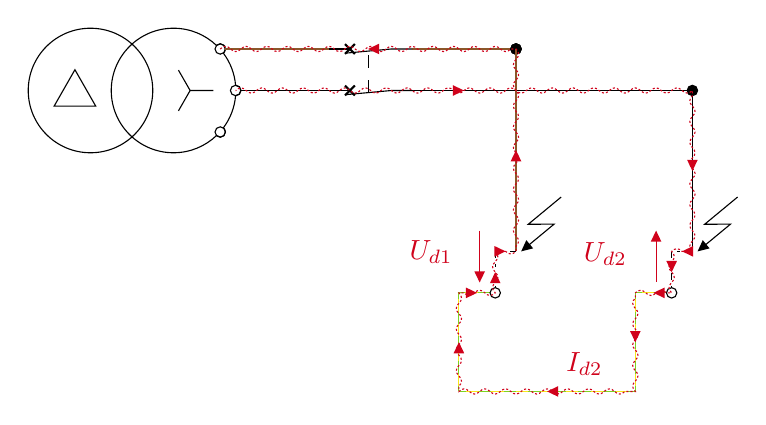
\begin{tikzpicture}[x=0.75pt,y=0.75pt,yscale=-1,xscale=1]
%uncomment if require: \path (0,219); %set diagram left start at 0, and has height of 219

%Straight Lines [id:da4511637283243949] 
\draw  [dash pattern={on 2.25pt off 2.25pt on 1pt off 2.25pt}]  (252.5,112.5) -- (242.5,112.5) -- (242.5,130) ;
%Straight Lines [id:da9527130819146642] 
\draw  [dash pattern={on 2.25pt off 2.25pt on 1pt off 2.25pt}]  (337.5,112.5) -- (327.5,112.5) -- (327.5,130) ;
%Straight Lines [id:da24126717784692808] 
\draw [color={rgb, 255:red, 0; green, 0; blue, 0 }  ,draw opacity=1 ]   (337.5,112.5) -- (337.5,35) ;
%Straight Lines [id:da3468467801372336] 
\draw    (202.5,35) -- (337.5,35) ;
%Straight Lines [id:da5563024891724297] 
\draw [color={rgb, 255:red, 139; green, 87; blue, 42 }  ,draw opacity=1 ]   (202.5,15) -- (252.5,15) ;
%Shape: Path Data [id:dp43837740322366014] 
\draw   (112.5,55) .. controls (112.5,56.38) and (111.38,57.5) .. (110,57.5) .. controls (109.29,57.5) and (108.65,57.2) .. (108.19,56.72) .. controls (102.81,61.85) and (95.52,65) .. (87.5,65) .. controls (70.93,65) and (57.5,51.57) .. (57.5,35) .. controls (57.5,18.43) and (70.93,5) .. (87.5,5) .. controls (95.52,5) and (102.81,8.15) .. (108.19,13.28) .. controls (108.65,12.8) and (109.29,12.5) .. (110,12.5) .. controls (111.38,12.5) and (112.5,13.62) .. (112.5,15) .. controls (112.5,15.82) and (112.11,16.54) .. (111.5,17) .. controls (114.8,21.39) and (116.92,26.71) .. (117.4,32.5) .. controls (117.43,32.5) and (117.47,32.5) .. (117.5,32.5) .. controls (118.88,32.5) and (120,33.62) .. (120,35) .. controls (120,36.38) and (118.88,37.5) .. (117.5,37.5) .. controls (117.47,37.5) and (117.43,37.5) .. (117.4,37.5) .. controls (116.92,43.29) and (114.8,48.61) .. (111.5,53) .. controls (112.11,53.46) and (112.5,54.18) .. (112.5,55) -- cycle ;
%Shape: Circle [id:dp03603482838008654] 
\draw   (17.5,35) .. controls (17.5,18.43) and (30.93,5) .. (47.5,5) .. controls (64.07,5) and (77.5,18.43) .. (77.5,35) .. controls (77.5,51.57) and (64.07,65) .. (47.5,65) .. controls (30.93,65) and (17.5,51.57) .. (17.5,35) -- cycle ;
%Shape: Triangle [id:dp7860018021593028] 
\draw   (40,25) -- (30,42.5) -- (50,42.5) -- cycle ;
%Shape: Star [id:dp36273195667205105] 
\draw   (106.75,35) -- (95.5,35) -- (89.88,44.81) -- (95.5,35) -- (89.88,25.19) -- (95.5,35) -- cycle ;
%Shape: Circle [id:dp581329576165861] 
\draw   (107.5,15) .. controls (107.5,13.62) and (108.62,12.5) .. (110,12.5) .. controls (111.38,12.5) and (112.5,13.62) .. (112.5,15) .. controls (112.5,16.38) and (111.38,17.5) .. (110,17.5) .. controls (108.62,17.5) and (107.5,16.38) .. (107.5,15) -- cycle ;
%Shape: Circle [id:dp008181652335233047] 
\draw   (114.9,35) .. controls (114.9,33.62) and (116.02,32.5) .. (117.4,32.5) .. controls (118.78,32.5) and (119.9,33.62) .. (119.9,35) .. controls (119.9,36.38) and (118.78,37.5) .. (117.4,37.5) .. controls (116.02,37.5) and (114.9,36.38) .. (114.9,35) -- cycle ;
%Shape: Circle [id:dp5428967410526352] 
\draw   (107.5,55) .. controls (107.5,53.62) and (108.62,52.5) .. (110,52.5) .. controls (111.38,52.5) and (112.5,53.62) .. (112.5,55) .. controls (112.5,56.38) and (111.38,57.5) .. (110,57.5) .. controls (108.62,57.5) and (107.5,56.38) .. (107.5,55) -- cycle ;

%Shape: Circle [id:dp3004196596154465] 
\draw  [fill={rgb, 255:red, 0; green, 0; blue, 0 }  ,fill opacity=1 ] (335,35) .. controls (335,33.62) and (336.12,32.5) .. (337.5,32.5) .. controls (338.88,32.5) and (340,33.62) .. (340,35) .. controls (340,36.38) and (338.88,37.5) .. (337.5,37.5) .. controls (336.12,37.5) and (335,36.38) .. (335,35) -- cycle ;
%Shape: Circle [id:dp38478162693673257] 
\draw  [fill={rgb, 255:red, 0; green, 0; blue, 0 }  ,fill opacity=1 ] (250,15) .. controls (250,13.62) and (251.12,12.5) .. (252.5,12.5) .. controls (253.88,12.5) and (255,13.62) .. (255,15) .. controls (255,16.38) and (253.88,17.5) .. (252.5,17.5) .. controls (251.12,17.5) and (250,16.38) .. (250,15) -- cycle ;
%Straight Lines [id:da35747201510733806] 
\draw [color={rgb, 255:red, 139; green, 87; blue, 42 }  ,draw opacity=1 ]   (112.5,15) -- (162.5,15) ;
%Straight Lines [id:da03938247690059582] 
\draw    (120,35) -- (162.5,35) ;
%Shape: Boxed Line [id:dp47312336425022783] 
\draw    (274.27,86.33) -- (258.39,99.47) -- (270.89,99.36) -- (257.31,110.59) ;
\draw [shift={(255,112.5)}, rotate = 320.40999999999997] [fill={rgb, 255:red, 0; green, 0; blue, 0 }  ][line width=0.08]  [draw opacity=0] (5.36,-2.57) -- (0,0) -- (5.36,2.57) -- cycle    ;
%Shape: Boxed Line [id:dp8604246706425941] 
\draw    (359.27,86.33) -- (343.39,99.47) -- (355.89,99.36) -- (342.31,110.59) ;
\draw [shift={(340,112.5)}, rotate = 320.40999999999997] [fill={rgb, 255:red, 0; green, 0; blue, 0 }  ][line width=0.08]  [draw opacity=0] (5.36,-2.57) -- (0,0) -- (5.36,2.57) -- cycle    ;
%Straight Lines [id:da6306782474143875] 
\draw    (170.5,37) -- (192.5,35) -- (202.5,35) ;
%Straight Lines [id:da4629224352649184] 
\draw    (172.5,35) -- (162.5,35) ;
\draw [shift={(172.5,35)}, rotate = 225] [color={rgb, 255:red, 0; green, 0; blue, 0 }  ][line width=0.75]    (-3.35,0) -- (3.35,0)(0,3.35) -- (0,-3.35)   ;
%Straight Lines [id:da5132783320552895] 
\draw    (170.5,17) -- (192.5,15) -- (202.5,15) ;
%Straight Lines [id:da123841191189479] 
\draw  [dash pattern={on 4.5pt off 4.5pt}]  (181.5,36) -- (181.5,16) ;
%Straight Lines [id:da38134434479229706] 
\draw    (172.5,15) -- (162.5,15) ;
\draw [shift={(172.5,15)}, rotate = 225] [color={rgb, 255:red, 0; green, 0; blue, 0 }  ][line width=0.75]    (-3.35,0) -- (3.35,0)(0,3.35) -- (0,-3.35)   ;

%Straight Lines [id:da029862379270012007] 
\draw [color={rgb, 255:red, 139; green, 87; blue, 42 }  ,draw opacity=1 ]   (252.5,112.5) -- (252.5,15) ;
%Shape: Circle [id:dp10157043967465573] 
\draw  [fill={rgb, 255:red, 0; green, 0; blue, 0 }  ,fill opacity=1 ] (250,15) .. controls (250,13.62) and (251.12,12.5) .. (252.5,12.5) .. controls (253.88,12.5) and (255,13.62) .. (255,15) .. controls (255,16.38) and (253.88,17.5) .. (252.5,17.5) .. controls (251.12,17.5) and (250,16.38) .. (250,15) -- cycle ;
%Shape: Circle [id:dp8079725241460669] 
\draw  [fill={rgb, 255:red, 0; green, 0; blue, 0 }  ,fill opacity=1 ] (250,15) .. controls (250,13.62) and (251.12,12.5) .. (252.5,12.5) .. controls (253.88,12.5) and (255,13.62) .. (255,15) .. controls (255,16.38) and (253.88,17.5) .. (252.5,17.5) .. controls (251.12,17.5) and (250,16.38) .. (250,15) -- cycle ;
%Straight Lines [id:da32787816985288987] 
\draw [color={rgb, 255:red, 208; green, 2; blue, 27 }  ,draw opacity=1 ]   (235,102.5) -- (235,124.5) ;
\draw [shift={(235,127.5)}, rotate = 270] [fill={rgb, 255:red, 208; green, 2; blue, 27 }  ,fill opacity=1 ][line width=0.08]  [draw opacity=0] (5.36,-2.57) -- (0,0) -- (5.36,2.57) -- cycle    ;
%Straight Lines [id:da9290035127505091] 
\draw [color={rgb, 255:red, 208; green, 2; blue, 27 }  ,draw opacity=1 ]   (320,105.5) -- (320,127.5) ;
\draw [shift={(320,102.5)}, rotate = 90] [fill={rgb, 255:red, 208; green, 2; blue, 27 }  ,fill opacity=1 ][line width=0.08]  [draw opacity=0] (5.36,-2.57) -- (0,0) -- (5.36,2.57) -- cycle    ;
%Straight Lines [id:da4236883272393758] 
\draw [color={rgb, 255:red, 248; green, 231; blue, 28 }  ,draw opacity=1 ]   (325,132.5) -- (310,132.5) -- (310,180) -- (225,180) ;
%Straight Lines [id:da1955939853197214] 
\draw [color={rgb, 255:red, 126; green, 211; blue, 33 }  ,draw opacity=1 ] [dash pattern={on 4.5pt off 4.5pt}]  (325,132.5) -- (310,132.5) -- (310,180) -- (225,180) ;
%Straight Lines [id:da8052192234703028] 
\draw [color={rgb, 255:red, 248; green, 231; blue, 28 }  ,draw opacity=1 ]   (240,132.5) -- (225,132.5) -- (225,180) ;
%Straight Lines [id:da6976347779102222] 
\draw [color={rgb, 255:red, 139; green, 87; blue, 42 }  ,draw opacity=1 ]   (252.5,110) -- (252.5,15) ;
%Straight Lines [id:da2970008681971681] 
\draw [color={rgb, 255:red, 126; green, 211; blue, 33 }  ,draw opacity=1 ] [dash pattern={on 4.5pt off 4.5pt}]  (240,132.5) -- (225,132.5) -- (225,180) ;
%Straight Lines [id:da7142618830255841] 
\draw [color={rgb, 255:red, 0; green, 0; blue, 0 }  ,draw opacity=1 ]   (337.5,110) -- (337.5,32.5) ;
%Shape: Circle [id:dp970057374964288] 
\draw  [fill={rgb, 255:red, 255; green, 255; blue, 255 }  ,fill opacity=1 ] (240,132.5) .. controls (240,131.12) and (241.12,130) .. (242.5,130) .. controls (243.88,130) and (245,131.12) .. (245,132.5) .. controls (245,133.88) and (243.88,135) .. (242.5,135) .. controls (241.12,135) and (240,133.88) .. (240,132.5) -- cycle ;
%Shape: Circle [id:dp5285112483449262] 
\draw  [fill={rgb, 255:red, 255; green, 255; blue, 255 }  ,fill opacity=1 ] (325,132.5) .. controls (325,131.12) and (326.12,130) .. (327.5,130) .. controls (328.88,130) and (330,131.12) .. (330,132.5) .. controls (330,133.88) and (328.88,135) .. (327.5,135) .. controls (326.12,135) and (325,133.88) .. (325,132.5) -- cycle ;
%Straight Lines [id:da2635484251048684] 
\draw [color={rgb, 255:red, 208; green, 2; blue, 27 }  ,draw opacity=1 ] [dash pattern={on 0.75pt off 0.75pt}]  (110,15) .. controls (111.67,13.33) and (113.33,13.33) .. (115,15) .. controls (116.67,16.67) and (118.33,16.67) .. (120,15) .. controls (121.67,13.33) and (123.33,13.33) .. (125,15) .. controls (126.67,16.67) and (128.33,16.67) .. (130,15) .. controls (131.67,13.33) and (133.33,13.33) .. (135,15) .. controls (136.67,16.67) and (138.33,16.67) .. (140,15) .. controls (141.67,13.33) and (143.33,13.33) .. (145,15) .. controls (146.67,16.67) and (148.33,16.67) .. (150,15) .. controls (151.67,13.33) and (153.33,13.33) .. (155,15) .. controls (156.67,16.67) and (158.33,16.67) .. (160,15) .. controls (161.67,13.33) and (163.33,13.33) .. (165,15) .. controls (166.67,16.67) and (168.33,16.67) .. (170,15) .. controls (171.67,13.33) and (173.33,13.33) .. (175,15) .. controls (176.67,16.67) and (178.33,16.67) .. (180,15) .. controls (181.67,13.33) and (183.33,13.33) .. (185,15) .. controls (186.67,16.67) and (188.33,16.67) .. (190,15) .. controls (191.67,13.33) and (193.33,13.33) .. (195,15) .. controls (196.67,16.67) and (198.33,16.67) .. (200,15) .. controls (201.67,13.33) and (203.33,13.33) .. (205,15) .. controls (206.67,16.67) and (208.33,16.67) .. (210,15) .. controls (211.67,13.33) and (213.33,13.33) .. (215,15) .. controls (216.67,16.67) and (218.33,16.67) .. (220,15) .. controls (221.67,13.33) and (223.33,13.33) .. (225,15) .. controls (226.67,16.67) and (228.33,16.67) .. (230,15) .. controls (231.67,13.33) and (233.33,13.33) .. (235,15) .. controls (236.67,16.67) and (238.33,16.67) .. (240,15) .. controls (241.67,13.33) and (243.33,13.33) .. (245,15) .. controls (246.67,16.67) and (248.33,16.67) .. (250,15) -- (252.5,15) -- (252.5,15) .. controls (254.17,16.67) and (254.17,18.33) .. (252.5,20) .. controls (250.83,21.67) and (250.83,23.33) .. (252.5,25) .. controls (254.17,26.67) and (254.17,28.33) .. (252.5,30) .. controls (250.83,31.67) and (250.83,33.33) .. (252.5,35) .. controls (254.17,36.67) and (254.17,38.33) .. (252.5,40) .. controls (250.83,41.67) and (250.83,43.33) .. (252.5,45) .. controls (254.17,46.67) and (254.17,48.33) .. (252.5,50) .. controls (250.83,51.67) and (250.83,53.33) .. (252.5,55) .. controls (254.17,56.67) and (254.17,58.33) .. (252.5,60) .. controls (250.83,61.67) and (250.83,63.33) .. (252.5,65) .. controls (254.17,66.67) and (254.17,68.33) .. (252.5,70) .. controls (250.83,71.67) and (250.83,73.33) .. (252.5,75) .. controls (254.17,76.67) and (254.17,78.33) .. (252.5,80) .. controls (250.83,81.67) and (250.83,83.33) .. (252.5,85) .. controls (254.17,86.67) and (254.17,88.33) .. (252.5,90) .. controls (250.83,91.67) and (250.83,93.33) .. (252.5,95) .. controls (254.17,96.67) and (254.17,98.33) .. (252.5,100) .. controls (250.83,101.67) and (250.83,103.33) .. (252.5,105) .. controls (254.17,106.67) and (254.17,108.33) .. (252.5,110) -- (252.5,112.5) -- (252.5,112.5) .. controls (250.83,114.17) and (249.17,114.17) .. (247.5,112.5) -- (242.5,112.5) -- (242.5,112.5) .. controls (244.17,114.17) and (244.17,115.83) .. (242.5,117.5) .. controls (240.83,119.17) and (240.83,120.83) .. (242.5,122.5) .. controls (244.17,124.17) and (244.17,125.83) .. (242.5,127.5) .. controls (240.83,129.17) and (240.83,130.83) .. (242.5,132.5) -- (242.5,132.5) .. controls (240.83,134.17) and (239.17,134.17) .. (237.5,132.5) .. controls (235.83,130.83) and (234.17,130.83) .. (232.5,132.5) .. controls (230.83,134.17) and (229.17,134.17) .. (227.5,132.5) -- (225,132.5) -- (225,132.5) .. controls (226.67,134.17) and (226.67,135.83) .. (225,137.5) .. controls (223.33,139.17) and (223.33,140.83) .. (225,142.5) .. controls (226.67,144.17) and (226.67,145.83) .. (225,147.5) .. controls (223.33,149.17) and (223.33,150.83) .. (225,152.5) .. controls (226.67,154.17) and (226.67,155.83) .. (225,157.5) .. controls (223.33,159.17) and (223.33,160.83) .. (225,162.5) .. controls (226.67,164.17) and (226.67,165.83) .. (225,167.5) .. controls (223.33,169.17) and (223.33,170.83) .. (225,172.5) .. controls (226.67,174.17) and (226.67,175.83) .. (225,177.5) -- (225,180) -- (225,180) .. controls (226.67,178.33) and (228.33,178.33) .. (230,180) .. controls (231.67,181.67) and (233.33,181.67) .. (235,180) .. controls (236.67,178.33) and (238.33,178.33) .. (240,180) .. controls (241.67,181.67) and (243.33,181.67) .. (245,180) .. controls (246.67,178.33) and (248.33,178.33) .. (250,180) .. controls (251.67,181.67) and (253.33,181.67) .. (255,180) .. controls (256.67,178.33) and (258.33,178.33) .. (260,180) .. controls (261.67,181.67) and (263.33,181.67) .. (265,180) .. controls (266.67,178.33) and (268.33,178.33) .. (270,180) .. controls (271.67,181.67) and (273.33,181.67) .. (275,180) .. controls (276.67,178.33) and (278.33,178.33) .. (280,180) .. controls (281.67,181.67) and (283.33,181.67) .. (285,180) .. controls (286.67,178.33) and (288.33,178.33) .. (290,180) .. controls (291.67,181.67) and (293.33,181.67) .. (295,180) .. controls (296.67,178.33) and (298.33,178.33) .. (300,180) .. controls (301.67,181.67) and (303.33,181.67) .. (305,180) -- (310,180) -- (310,180) .. controls (308.33,178.33) and (308.33,176.67) .. (310,175) .. controls (311.67,173.33) and (311.67,171.67) .. (310,170) .. controls (308.33,168.33) and (308.33,166.67) .. (310,165) .. controls (311.67,163.33) and (311.67,161.67) .. (310,160) .. controls (308.33,158.33) and (308.33,156.67) .. (310,155) .. controls (311.67,153.33) and (311.67,151.67) .. (310,150) .. controls (308.33,148.33) and (308.33,146.67) .. (310,145) .. controls (311.67,143.33) and (311.67,141.67) .. (310,140) .. controls (308.33,138.33) and (308.33,136.67) .. (310,135) -- (310,132.5) -- (310,132.5) .. controls (311.67,130.83) and (313.33,130.83) .. (315,132.5) .. controls (316.67,134.17) and (318.33,134.17) .. (320,132.5) .. controls (321.67,130.83) and (323.33,130.83) .. (325,132.5) -- (327.5,132.5) -- (327.5,132.5) .. controls (325.83,130.83) and (325.83,129.17) .. (327.5,127.5) .. controls (329.17,125.83) and (329.17,124.17) .. (327.5,122.5) .. controls (325.83,120.83) and (325.83,119.17) .. (327.5,117.5) .. controls (329.17,115.83) and (329.17,114.17) .. (327.5,112.5) -- (327.5,112.5) .. controls (329.17,110.83) and (330.83,110.83) .. (332.5,112.5) -- (337.5,112.5) -- (337.5,112.5) .. controls (335.83,110.83) and (335.83,109.17) .. (337.5,107.5) .. controls (339.17,105.83) and (339.17,104.17) .. (337.5,102.5) .. controls (335.83,100.83) and (335.83,99.17) .. (337.5,97.5) .. controls (339.17,95.83) and (339.17,94.17) .. (337.5,92.5) .. controls (335.83,90.83) and (335.83,89.17) .. (337.5,87.5) .. controls (339.17,85.83) and (339.17,84.17) .. (337.5,82.5) .. controls (335.83,80.83) and (335.83,79.17) .. (337.5,77.5) .. controls (339.17,75.83) and (339.17,74.17) .. (337.5,72.5) .. controls (335.83,70.83) and (335.83,69.17) .. (337.5,67.5) .. controls (339.17,65.83) and (339.17,64.17) .. (337.5,62.5) .. controls (335.83,60.83) and (335.83,59.17) .. (337.5,57.5) .. controls (339.17,55.83) and (339.17,54.17) .. (337.5,52.5) .. controls (335.83,50.83) and (335.83,49.17) .. (337.5,47.5) .. controls (339.17,45.83) and (339.17,44.17) .. (337.5,42.5) .. controls (335.83,40.83) and (335.83,39.17) .. (337.5,37.5) -- (337.5,35) -- (337.5,35) .. controls (335.83,36.67) and (334.17,36.67) .. (332.5,35) .. controls (330.83,33.33) and (329.17,33.33) .. (327.5,35) .. controls (325.83,36.67) and (324.17,36.67) .. (322.5,35) .. controls (320.83,33.33) and (319.17,33.33) .. (317.5,35) .. controls (315.83,36.67) and (314.17,36.67) .. (312.5,35) .. controls (310.83,33.33) and (309.17,33.33) .. (307.5,35) .. controls (305.83,36.67) and (304.17,36.67) .. (302.5,35) .. controls (300.83,33.33) and (299.17,33.33) .. (297.5,35) .. controls (295.83,36.67) and (294.17,36.67) .. (292.5,35) .. controls (290.83,33.33) and (289.17,33.33) .. (287.5,35) .. controls (285.83,36.67) and (284.17,36.67) .. (282.5,35) .. controls (280.83,33.33) and (279.17,33.33) .. (277.5,35) .. controls (275.83,36.67) and (274.17,36.67) .. (272.5,35) .. controls (270.83,33.33) and (269.17,33.33) .. (267.5,35) .. controls (265.83,36.67) and (264.17,36.67) .. (262.5,35) .. controls (260.83,33.33) and (259.17,33.33) .. (257.5,35) .. controls (255.83,36.67) and (254.17,36.67) .. (252.5,35) .. controls (250.83,33.33) and (249.17,33.33) .. (247.5,35) .. controls (245.83,36.67) and (244.17,36.67) .. (242.5,35) .. controls (240.83,33.33) and (239.17,33.33) .. (237.5,35) .. controls (235.83,36.67) and (234.17,36.67) .. (232.5,35) .. controls (230.83,33.33) and (229.17,33.33) .. (227.5,35) .. controls (225.83,36.67) and (224.17,36.67) .. (222.5,35) .. controls (220.83,33.33) and (219.17,33.33) .. (217.5,35) .. controls (215.83,36.67) and (214.17,36.67) .. (212.5,35) .. controls (210.83,33.33) and (209.17,33.33) .. (207.5,35) .. controls (205.83,36.67) and (204.17,36.67) .. (202.5,35) .. controls (200.83,33.33) and (199.17,33.33) .. (197.5,35) .. controls (195.83,36.67) and (194.17,36.67) .. (192.5,35) .. controls (190.83,33.33) and (189.17,33.33) .. (187.5,35) .. controls (185.83,36.67) and (184.17,36.67) .. (182.5,35) .. controls (180.83,33.33) and (179.17,33.33) .. (177.5,35) .. controls (175.83,36.67) and (174.17,36.67) .. (172.5,35) .. controls (170.83,33.33) and (169.17,33.33) .. (167.5,35) .. controls (165.83,36.67) and (164.17,36.67) .. (162.5,35) .. controls (160.83,33.33) and (159.17,33.33) .. (157.5,35) .. controls (155.83,36.67) and (154.17,36.67) .. (152.5,35) .. controls (150.83,33.33) and (149.17,33.33) .. (147.5,35) .. controls (145.83,36.67) and (144.17,36.67) .. (142.5,35) .. controls (140.83,33.33) and (139.17,33.33) .. (137.5,35) .. controls (135.83,36.67) and (134.17,36.67) .. (132.5,35) .. controls (130.83,33.33) and (129.17,33.33) .. (127.5,35) .. controls (125.83,36.67) and (124.17,36.67) .. (122.5,35) .. controls (120.83,33.33) and (119.17,33.33) .. (117.5,35) -- (117.4,35) -- (117.4,35) ;
\draw [shift={(181.25,15)}, rotate = 0] [fill={rgb, 255:red, 208; green, 2; blue, 27 }  ,fill opacity=1 ][line width=0.08]  [draw opacity=0] (5.36,-2.57) -- (0,0) -- (5.36,2.57) -- cycle    ;
\draw [shift={(252.5,63.75)}, rotate = 90] [fill={rgb, 255:red, 208; green, 2; blue, 27 }  ,fill opacity=1 ][line width=0.08]  [draw opacity=0] (5.36,-2.57) -- (0,0) -- (5.36,2.57) -- cycle    ;
\draw [shift={(247.5,112.5)}, rotate = 180] [fill={rgb, 255:red, 208; green, 2; blue, 27 }  ,fill opacity=1 ][line width=0.08]  [draw opacity=0] (5.36,-2.57) -- (0,0) -- (5.36,2.57) -- cycle    ;
\draw [shift={(242.5,122.5)}, rotate = 90] [fill={rgb, 255:red, 208; green, 2; blue, 27 }  ,fill opacity=1 ][line width=0.08]  [draw opacity=0] (5.36,-2.57) -- (0,0) -- (5.36,2.57) -- cycle    ;
\draw [shift={(233.75,132.5)}, rotate = 180] [fill={rgb, 255:red, 208; green, 2; blue, 27 }  ,fill opacity=1 ][line width=0.08]  [draw opacity=0] (5.36,-2.57) -- (0,0) -- (5.36,2.57) -- cycle    ;
\draw [shift={(225,156.25)}, rotate = 90] [fill={rgb, 255:red, 208; green, 2; blue, 27 }  ,fill opacity=1 ][line width=0.08]  [draw opacity=0] (5.36,-2.57) -- (0,0) -- (5.36,2.57) -- cycle    ;
\draw [shift={(267.5,180)}, rotate = 0] [fill={rgb, 255:red, 208; green, 2; blue, 27 }  ,fill opacity=1 ][line width=0.08]  [draw opacity=0] (5.36,-2.57) -- (0,0) -- (5.36,2.57) -- cycle    ;
\draw [shift={(310,156.25)}, rotate = 270] [fill={rgb, 255:red, 208; green, 2; blue, 27 }  ,fill opacity=1 ][line width=0.08]  [draw opacity=0] (5.36,-2.57) -- (0,0) -- (5.36,2.57) -- cycle    ;
\draw [shift={(318.75,132.5)}, rotate = 0] [fill={rgb, 255:red, 208; green, 2; blue, 27 }  ,fill opacity=1 ][line width=0.08]  [draw opacity=0] (5.36,-2.57) -- (0,0) -- (5.36,2.57) -- cycle    ;
\draw [shift={(327.5,122.5)}, rotate = 270] [fill={rgb, 255:red, 208; green, 2; blue, 27 }  ,fill opacity=1 ][line width=0.08]  [draw opacity=0] (5.36,-2.57) -- (0,0) -- (5.36,2.57) -- cycle    ;
\draw [shift={(332.5,112.5)}, rotate = 0] [fill={rgb, 255:red, 208; green, 2; blue, 27 }  ,fill opacity=1 ][line width=0.08]  [draw opacity=0] (5.36,-2.57) -- (0,0) -- (5.36,2.57) -- cycle    ;
\draw [shift={(337.5,73.75)}, rotate = 270] [fill={rgb, 255:red, 208; green, 2; blue, 27 }  ,fill opacity=1 ][line width=0.08]  [draw opacity=0] (5.36,-2.57) -- (0,0) -- (5.36,2.57) -- cycle    ;
\draw [shift={(227.45,35)}, rotate = 180] [fill={rgb, 255:red, 208; green, 2; blue, 27 }  ,fill opacity=1 ][line width=0.08]  [draw opacity=0] (5.36,-2.57) -- (0,0) -- (5.36,2.57) -- cycle    ;


% Text Node
\draw (275.5,160) node [anchor=north west][inner sep=0.75pt]  [color={rgb, 255:red, 208; green, 2; blue, 27 }  ,opacity=1 ] [align=left] {$I_{d2}$};
% Text Node
\draw (200,106) node [anchor=north west][inner sep=0.75pt]  [color={rgb, 255:red, 208; green, 2; blue, 27 }  ,opacity=1 ] [align=left] {$U_{d1}$};
% Text Node
\draw (284,107) node [anchor=north west][inner sep=0.75pt]  [color={rgb, 255:red, 208; green, 2; blue, 27 }  ,opacity=1 ] [align=left] {$U_{d2}$};


\end{tikzpicture}


\end{figure}

%\end{document}


L'intensité de courant $I_{d2}$ vaut alors :
\begin{formule}[Courant du deuxième défaut $I_{d2}$ en schéma Isolé-Interconnecté]
\begin{align*}
		I_{d2} &= \frac{0,5 \times U}{R_{ph1}+R_{ph2}} \\
\end{align*}
\end{formule}

\begin{textvariables}
U								& tension nominale composée				& volt			& \volt					& 	Différence de potentiel entre deux conducteurs actifs (à préciser s'il s'agit du conducteur neutre)	\\
R_{ph1}					& résistance											& ohm			& \ohm					& 	Résistance de du conducteur actif alimentant l'appareil 1\\
R_{ph2}					& résistance											& ohm			& \ohm					& 	Résistance de du conducteur actif alimentant l'appareil 2\\
\end{textvariables}

Le courant de défaut $I_{d1}$ fera alors apparaître une \emph{tension de défaut} $U_{d}$ entre la masse métallique de l'appareil 1 et la masse métallique de l'appareil 2. \\
On néglige également la résistance du conducteur PE devant celle des phases. Dans ce contexte-là, la tension de défaut $U_d$ vaut alors :

\begin{formule}[Tension de défaut $U_{d}$ en schéma Isolé-Individuel]
\begin{align*}
		U_{d} &= \frac{0,5 \times U}{2} \\
\end{align*}
\end{formule}

\begin{textvariables}
U								& tension nominale composée				& volt			& \volt					& 	Différence de potentiel entre deux conducteurs actifs (à préciser s'il s'agit du conducteur neutre)	\\
I_{d2}						& intensité												& ampère		& \ampere				& 	Courant de défaut de l'appareil 2 \\
U_{L}						& tension							& volt			& \volt										& 	Tension de sécurité du local avec :
\begin{description}[nosep, leftmargin=*]
\item[Local sec :] $U_{L}=\SI{50}{\volt}$
\item[Local humide :] $U_{L}=\SI{25}{\volt}$
\end{description} \\
\end{textvariables}

Cette tension de défaut est dangereuse et il faut obligatoirement couper l'alimentation en protégeant les circuits par des disjoncteurs magnéto-thermique, qui doivent respecter les temps de coupure suivant :

%--------------------------------------
%ELECTROTECHNIQUE - SCHEMA DE LIAISON A LA TERRE
%--------------------------------------

%utiliser les environnement \begin{comment} \end{comment} pour mettre en commentaire le préambule une fois la programmation appelée dans le document maître (!ne pas oublier de mettre en commentaire \end{document}!)

\begin{comment}

\documentclass[a4paper, 11pt, twoside, fleqn]{memoir}

\usepackage{AOCDTF}

\marqueurchapitre
\decoupagechapitre{1} %juste pour éviter les erreurs lors de la compilation des sous-programmations (passera en commentaire)

%lien d'édition des figures Tikz sur le site mathcha.io (rajouter le lien d'une modification effectuée sur la figure tikz avec le nom du modificateur car il n'y a qu'un lien par compte)

%lien éditeur Bruno Douchy : https://www.mathcha.io/editor/zjygnFElSdyhJ72e3zT5ZgqwBT4DKnovswpXn1q

%--------------------------------------
%corps du document
%--------------------------------------

\begin{document} %corps du document
	\openleft %début de chapitre à gauche

\end{comment}

\begin{table}[H]
\caption{Temps de coupure maximal des disjoncteurs en schéma IT\label{tab:schema_it_temps_coupure}}
\begin{threeparttable} %note dans tableau
\begin{tabularx}{\textwidth}{C C C}
\toprule
\multirow[c]{2}{*}{\thead{Réseaux usuels}} & \multicolumn{2}{c}{\thead{Temps de coupure maximal (\si{\milli\second})}}\\
\cmidrule(lr){2-3} 
	& $U_{L}=\SI{50}{\volt}$ 	& 			$U_{L}=\SI{25}{\volt}$  \\
\midrule
\multicolumn{3}{l}{\textit{Neutre non distribué}} \\
\middashrule
\SI{127}{\volt}/\SI{230}{\volt}		& 800		& 400 \\
\SI{230}{\volt}/\SI{400}{\volt}		& 400		& 200 \\
\SI{400}{\volt}/\SI{690}{\volt}		& 200		& 60 \\
\SI{690}{\volt}/\SI{1000}{\volt}	& 100		& 20 \\
\addlinespace
\multicolumn{3}{l}{\textit{Neutre distribué\tnote{1}}} \\
\middashrule
\SI{127}{\volt}/\SI{230}{\volt}		& 5000		& 1000 \\
\SI{230}{\volt}/\SI{400}{\volt}		& 800		& 500 \\
\SI{400}{\volt}/\SI{690}{\volt}		& 400		& 200 \\
\SI{690}{\volt}/\SI{1000}{\volt}	& 200		& 80 \\
\bottomrule 
\end{tabularx}
\begin{tablenotes}
    \item[1] les installations monophasées sont considérées comme des installations à neutre distribué.
\end{tablenotes}
\end{threeparttable} %note dans tableau
\end{table}

%\end{document}



La longueur maximale des conducteurs en schéma IT avec les masses interconnectées se calculent avec les mêmes méthodes que pour les installations en schéma TN (voir \superref{sec:schema_tn_methode_conventionnelle}).

\section{Contrôle permanent de l'installation en schéma IT}

Quand l'installation électrique est en schéma IT, il est nécessaire d'avoir une équipe de maintenance à disposition pour intervenir rapidement en cas de premier défaut. Pour les détecter au plus vite, il faut installer un Contrôleur Permanent d'Isolement (CPI). Il s'agit d'un appareil placé en dérivation qui va calculer en permanence deux paramètres de l'installation :
\begin{description}
\item[\Circled{1} niveau d'isolement général $Z_{res}$ :] injection d'une tension (continue ou alternative de basse fréquence) entre le neutre et la terre, générant un \emph{courant de fuite} $I_f$ dont l'intensité sera proportionnellement inverse au niveau d'isolement général de l'installation électrique. Au-dessous d'un certain seuil d'isolement réglable (généralement entre \numrange{0,7}{100}\si{\kilo\ohm}), le CPI déclenche une alarme. 
\item[\Circled{2} apparition d'un défaut franc sur un circuit :] installation de tores de détection sur les circuits à surveiller, calculant la différence entre le courant entre et sortant (mécanisme similaire à ceux des DDR). Cela permet de localiser précisément les circuits en défaut.
\end{description} 

 \begin{figure}[H]
\caption{Installation Isolé-Individuelle avec CPI}
\begin{subfigure}[t]{0.49\linewidth}
%--------------------------------------
%ELECTROTECHNIQUE - SCHEMA DE LIAISON A LA TERRE
%--------------------------------------

%utiliser les environnement \begin{comment} \end{comment} pour mettre en commentaire le préambule une fois la programmation appelée dans le document maître (!ne pas oublier de mettre en commentaire \end{document}!)

\begin{comment}

\documentclass[a4paper, 11pt, twoside, fleqn]{memoir}

\usepackage{AOCDTF}

\marqueurchapitre
\decoupagechapitre{1} %juste pour éviter les erreurs lors de la compilation des sous-programmations (passera en commentaire)

%lien d'édition des figures Tikz sur le site mathcha.io (rajouter le lien d'une modification effectuée sur la figure tikz avec le nom du modificateur car il n'y a qu'un lien par compte)

%lien mathcha Bruno Douchy : https://www.mathcha.io/editor/jQKLoCODsYQuv6lo9wh5LQq3pSzO0mydSnpzwBy

%--------------------------------------
%corps du document
%--------------------------------------

\begin{document} %corps du document
	\openleft %début de chapitre à gauche

\end{comment}

% Pattern Info
 
\tikzset{
pattern size/.store in=\mcSize, 
pattern size = 5pt,
pattern thickness/.store in=\mcThickness, 
pattern thickness = 0.3pt,
pattern radius/.store in=\mcRadius, 
pattern radius = 1pt}
\makeatletter
\pgfutil@ifundefined{pgf@pattern@name@_l7ih23hqm}{
\pgfdeclarepatternformonly[\mcThickness,\mcSize]{_l7ih23hqm}
{\pgfqpoint{0pt}{0pt}}
{\pgfpoint{\mcSize+\mcThickness}{\mcSize+\mcThickness}}
{\pgfpoint{\mcSize}{\mcSize}}
{
\pgfsetcolor{\tikz@pattern@color}
\pgfsetlinewidth{\mcThickness}
\pgfpathmoveto{\pgfqpoint{0pt}{0pt}}
\pgfpathlineto{\pgfpoint{\mcSize+\mcThickness}{\mcSize+\mcThickness}}
\pgfusepath{stroke}
}}
\makeatother
\tikzset{every picture/.style={line width=0.5pt}} %set default line width to 0.75pt        

\begin{tikzpicture}[x=0.75pt,y=0.75pt,yscale=-0.6,xscale=0.6]
%uncomment if require: \path (0,320); %set diagram left start at 0, and has height of 320

%Shape: Rectangle [id:dp9736059741519228] 
\draw  [dash pattern={on 2.25pt off 2.25pt on 1pt off 2.25pt}] (242.5,160) -- (302.5,160) -- (302.5,190) -- (242.5,190) -- cycle ;
%Shape: Rectangle [id:dp6541068284877478] 
\draw  [dash pattern={on 2.25pt off 2.25pt on 1pt off 2.25pt}] (327.5,160) -- (387.5,160) -- (387.5,190) -- (327.5,190) -- cycle ;
%Shape: Rectangle [id:dp28129735245298193] 
\draw  [dash pattern={on 2.25pt off 2.25pt on 1pt off 2.25pt}] (412.5,160) -- (472.5,160) -- (472.5,190) -- (412.5,190) -- cycle ;
%Straight Lines [id:da4922757986185987] 
\draw [color={rgb, 255:red, 74; green, 144; blue, 226 }  ,draw opacity=1 ]   (152.5,75) -- (162.5,75) ;
%Straight Lines [id:da4038713220143262] 
\draw [color={rgb, 255:red, 74; green, 144; blue, 226 }  ,draw opacity=1 ]   (462.5,175) -- (462.5,155) ;
%Straight Lines [id:da9166454765790462] 
\draw [color={rgb, 255:red, 74; green, 144; blue, 226 }  ,draw opacity=1 ]   (462.5,107.5) -- (462.5,77.5) ;
%Straight Lines [id:da9023577986083069] 
\draw [color={rgb, 255:red, 74; green, 144; blue, 226 }  ,draw opacity=1 ]   (377.5,175) -- (377.5,155) ;
%Straight Lines [id:da5928803977736146] 
\draw [color={rgb, 255:red, 74; green, 144; blue, 226 }  ,draw opacity=1 ]   (377.5,107.5) -- (377.5,77.5) ;
%Straight Lines [id:da30570583399348505] 
\draw [color={rgb, 255:red, 74; green, 144; blue, 226 }  ,draw opacity=1 ]   (292.5,175) -- (292.5,155) ;
%Straight Lines [id:da8819404575351564] 
\draw [color={rgb, 255:red, 139; green, 87; blue, 42 }  ,draw opacity=1 ]   (252.5,175) -- (252.5,155) ;
%Straight Lines [id:da28367841763640167] 
\draw [color={rgb, 255:red, 155; green, 155; blue, 155 }  ,draw opacity=1 ]   (422.5,175) -- (422.5,155) ;
%Straight Lines [id:da6880263813112385] 
\draw [color={rgb, 255:red, 0; green, 0; blue, 0 }  ,draw opacity=1 ]   (337.5,175) -- (337.5,152.5) ;
%Straight Lines [id:da8972215794381513] 
\draw [color={rgb, 255:red, 248; green, 231; blue, 28 }  ,draw opacity=1 ]   (87.5,75) -- (27.5,75) -- (27.5,182.5) ;
%Straight Lines [id:da07998178544200962] 
\draw [color={rgb, 255:red, 248; green, 231; blue, 28 }  ,draw opacity=1 ]   (95.5,35) -- (87.5,75) -- (87.5,107.5) ;
%Straight Lines [id:da7929766229120194] 
\draw [color={rgb, 255:red, 126; green, 211; blue, 33 }  ,draw opacity=1 ] [dash pattern={on 2.25pt off 2.25pt}]  (95.5,35) -- (87.5,75) -- (87.5,107.5) ;
%Straight Lines [id:da4949912109010227] 
\draw [color={rgb, 255:red, 74; green, 144; blue, 226 }  ,draw opacity=1 ]   (202.5,75) -- (460,75) ;
%Straight Lines [id:da7560950775201385] 
\draw [color={rgb, 255:red, 248; green, 231; blue, 28 }  ,draw opacity=1 ]   (240,180) -- (225,180) -- (225,182.5) ;
%Straight Lines [id:da49944531942669546] 
\draw    (202.5,35) -- (462.5,35) ;
%Straight Lines [id:da47196191445949953] 
\draw [color={rgb, 255:red, 139; green, 87; blue, 42 }  ,draw opacity=1 ]   (202.5,15) -- (462.5,15) ;
%Straight Lines [id:da034038054075003044] 
\draw [color={rgb, 255:red, 155; green, 155; blue, 155 }  ,draw opacity=1 ]   (202.5,55) -- (462.5,55) ;
%Shape: Path Data [id:dp09879682351014718] 
\draw   (112.5,55) .. controls (112.5,56.38) and (111.38,57.5) .. (110,57.5) .. controls (109.29,57.5) and (108.65,57.2) .. (108.19,56.72) .. controls (102.81,61.85) and (95.52,65) .. (87.5,65) .. controls (70.93,65) and (57.5,51.57) .. (57.5,35) .. controls (57.5,18.43) and (70.93,5) .. (87.5,5) .. controls (95.52,5) and (102.81,8.15) .. (108.19,13.28) .. controls (108.65,12.8) and (109.29,12.5) .. (110,12.5) .. controls (111.38,12.5) and (112.5,13.62) .. (112.5,15) .. controls (112.5,15.82) and (112.11,16.54) .. (111.5,17) .. controls (114.8,21.39) and (116.92,26.71) .. (117.4,32.5) .. controls (117.43,32.5) and (117.47,32.5) .. (117.5,32.5) .. controls (118.88,32.5) and (120,33.62) .. (120,35) .. controls (120,36.38) and (118.88,37.5) .. (117.5,37.5) .. controls (117.47,37.5) and (117.43,37.5) .. (117.4,37.5) .. controls (116.92,43.29) and (114.8,48.61) .. (111.5,53) .. controls (112.11,53.46) and (112.5,54.18) .. (112.5,55) -- cycle ;
%Shape: Circle [id:dp09395491014356527] 
\draw   (17.5,35) .. controls (17.5,18.43) and (30.93,5) .. (47.5,5) .. controls (64.07,5) and (77.5,18.43) .. (77.5,35) .. controls (77.5,51.57) and (64.07,65) .. (47.5,65) .. controls (30.93,65) and (17.5,51.57) .. (17.5,35) -- cycle ;
%Shape: Triangle [id:dp01558250765431457] 
\draw   (40,25) -- (30,42.5) -- (50,42.5) -- cycle ;
%Shape: Star [id:dp0013707252732991781] 
\draw   (106.75,35) -- (95.5,35) -- (89.88,44.81) -- (95.5,35) -- (89.88,25.19) -- (95.5,35) -- cycle ;
%Shape: Circle [id:dp39893592802184263] 
\draw   (107.5,15) .. controls (107.5,13.62) and (108.62,12.5) .. (110,12.5) .. controls (111.38,12.5) and (112.5,13.62) .. (112.5,15) .. controls (112.5,16.38) and (111.38,17.5) .. (110,17.5) .. controls (108.62,17.5) and (107.5,16.38) .. (107.5,15) -- cycle ;
%Shape: Circle [id:dp9893284041115082] 
\draw   (114.9,35) .. controls (114.9,33.62) and (116.02,32.5) .. (117.4,32.5) .. controls (118.78,32.5) and (119.9,33.62) .. (119.9,35) .. controls (119.9,36.38) and (118.78,37.5) .. (117.4,37.5) .. controls (116.02,37.5) and (114.9,36.38) .. (114.9,35) -- cycle ;
%Shape: Circle [id:dp3917292266620266] 
\draw   (107.5,55) .. controls (107.5,53.62) and (108.62,52.5) .. (110,52.5) .. controls (111.38,52.5) and (112.5,53.62) .. (112.5,55) .. controls (112.5,56.38) and (111.38,57.5) .. (110,57.5) .. controls (108.62,57.5) and (107.5,56.38) .. (107.5,55) -- cycle ;

%Straight Lines [id:da8322026187642189] 
\draw [color={rgb, 255:red, 139; green, 87; blue, 42 }  ,draw opacity=1 ]   (252.5,107.5) -- (252.5,15) ;
%Straight Lines [id:da8041249564118628] 
\draw [color={rgb, 255:red, 74; green, 144; blue, 226 }  ,draw opacity=1 ]   (292.5,107.5) -- (292.5,77.5) ;
%Straight Lines [id:da6342365727576158] 
\draw    (17.5,232.5) -- (460,232.5) ;
%Shape: Rectangle [id:dp8835182839666373] 
\draw  [draw opacity=0][pattern=_l7ih23hqm,pattern size=6pt,pattern thickness=0.75pt,pattern radius=0pt, pattern color={rgb, 255:red, 0; green, 0; blue, 0}][line width=0.75]  (17.5,232.5) -- (460,232.5) -- (460,247.5) -- (17.5,247.5) -- cycle ;
%Straight Lines [id:da658767187431958] 
\draw [color={rgb, 255:red, 126; green, 211; blue, 33 }  ,draw opacity=1 ] [dash pattern={on 2.25pt off 2.25pt}]  (240,180) -- (225,180) -- (225,182.5) ;
%Straight Lines [id:da06637251377195108] 
\draw [color={rgb, 255:red, 248; green, 231; blue, 28 }  ,draw opacity=1 ]   (225,222.5) -- (225,247.5) ;
%Straight Lines [id:da47233881321451787] 
\draw    (225,247.5) -- (225,262.5) ;
%Straight Lines [id:da5035312706678949] 
\draw    (215,262.5) -- (235,262.5) ;
%Straight Lines [id:da18116556144696694] 
\draw    (217.5,267.5) -- (232.5,267.5) ;
%Straight Lines [id:da26663321343914415] 
\draw    (220,272.5) -- (230,272.5) ;

%Straight Lines [id:da7788639142047531] 
\draw [color={rgb, 255:red, 126; green, 211; blue, 33 }  ,draw opacity=1 ] [dash pattern={on 2.25pt off 2.25pt}]  (225,222.5) -- (225,247.5) ;
%Straight Lines [id:da8201802660928923] 
\draw    (287.5,175) -- (292.5,175) ;
%Shape: Rectangle [id:dp3438336194943209] 
\draw   (257.5,170) -- (287.5,170) -- (287.5,180) -- (257.5,180) -- cycle ;
%Straight Lines [id:da27605197781986657] 
\draw    (252.5,175) -- (257.5,175) ;

%Straight Lines [id:da9011697570747588] 
\draw    (225,217.5) -- (225,222.5) ;
%Shape: Rectangle [id:dp36989703847460553] 
\draw   (230,187.5) -- (230,217.5) -- (220,217.5) -- (220,187.5) -- cycle ;
%Straight Lines [id:da6366900985555619] 
\draw    (225,182.5) -- (225,187.5) ;

%Straight Lines [id:da3812281827541767] 
\draw [color={rgb, 255:red, 0; green, 0; blue, 0 }  ,draw opacity=1 ]   (337.5,107.5) -- (337.5,37.5) ;
%Straight Lines [id:da02888103671964104] 
\draw    (372.5,175) -- (377.5,175) ;
%Shape: Rectangle [id:dp39971735208919124] 
\draw   (342.5,170) -- (372.5,170) -- (372.5,180) -- (342.5,180) -- cycle ;
%Straight Lines [id:da15610963345624862] 
\draw    (337.5,175) -- (342.5,175) ;

%Straight Lines [id:da7566594469565104] 
\draw [color={rgb, 255:red, 155; green, 155; blue, 155 }  ,draw opacity=1 ]   (422.5,107.5) -- (422.5,57.5) ;
%Straight Lines [id:da9791907804470615] 
\draw [color={rgb, 255:red, 74; green, 144; blue, 226 }  ,draw opacity=1 ]   (462.5,175.5) -- (462.5,162.5) ;
%Straight Lines [id:da15543680976570695] 
\draw    (457.5,175) -- (462.5,175) ;
%Shape: Rectangle [id:dp27259637225024935] 
\draw   (427.5,170) -- (457.5,170) -- (457.5,180) -- (427.5,180) -- cycle ;
%Straight Lines [id:da6590266150100259] 
\draw    (422.5,175) -- (427.5,175) ;

%Shape: Circle [id:dp3040137945437842] 
\draw  [fill={rgb, 255:red, 0; green, 0; blue, 0 }  ,fill opacity=1 ] (375,75) .. controls (375,73.62) and (376.12,72.5) .. (377.5,72.5) .. controls (378.88,72.5) and (380,73.62) .. (380,75) .. controls (380,76.38) and (378.88,77.5) .. (377.5,77.5) .. controls (376.12,77.5) and (375,76.38) .. (375,75) -- cycle ;
%Shape: Circle [id:dp5886475323071111] 
\draw  [fill={rgb, 255:red, 0; green, 0; blue, 0 }  ,fill opacity=1 ] (460,75) .. controls (460,73.62) and (461.12,72.5) .. (462.5,72.5) .. controls (463.88,72.5) and (465,73.62) .. (465,75) .. controls (465,76.38) and (463.88,77.5) .. (462.5,77.5) .. controls (461.12,77.5) and (460,76.38) .. (460,75) -- cycle ;
%Shape: Circle [id:dp7341854734672731] 
\draw  [fill={rgb, 255:red, 0; green, 0; blue, 0 }  ,fill opacity=1 ] (335,35) .. controls (335,33.62) and (336.12,32.5) .. (337.5,32.5) .. controls (338.88,32.5) and (340,33.62) .. (340,35) .. controls (340,36.38) and (338.88,37.5) .. (337.5,37.5) .. controls (336.12,37.5) and (335,36.38) .. (335,35) -- cycle ;
%Shape: Circle [id:dp6336551833672776] 
\draw  [fill={rgb, 255:red, 0; green, 0; blue, 0 }  ,fill opacity=1 ] (420,55) .. controls (420,53.62) and (421.12,52.5) .. (422.5,52.5) .. controls (423.88,52.5) and (425,53.62) .. (425,55) .. controls (425,56.38) and (423.88,57.5) .. (422.5,57.5) .. controls (421.12,57.5) and (420,56.38) .. (420,55) -- cycle ;
%Shape: Circle [id:dp5716316243984012] 
\draw  [fill={rgb, 255:red, 0; green, 0; blue, 0 }  ,fill opacity=1 ] (290,75) .. controls (290,73.62) and (291.12,72.5) .. (292.5,72.5) .. controls (293.88,72.5) and (295,73.62) .. (295,75) .. controls (295,76.38) and (293.88,77.5) .. (292.5,77.5) .. controls (291.12,77.5) and (290,76.38) .. (290,75) -- cycle ;
%Shape: Circle [id:dp9134099794169516] 
\draw  [fill={rgb, 255:red, 0; green, 0; blue, 0 }  ,fill opacity=1 ] (250,15) .. controls (250,13.62) and (251.12,12.5) .. (252.5,12.5) .. controls (253.88,12.5) and (255,13.62) .. (255,15) .. controls (255,16.38) and (253.88,17.5) .. (252.5,17.5) .. controls (251.12,17.5) and (250,16.38) .. (250,15) -- cycle ;
%Shape: Circle [id:dp314574850816974] 
\draw  [fill={rgb, 255:red, 255; green, 255; blue, 255 }  ,fill opacity=1 ] (240,180) .. controls (240,178.62) and (241.12,177.5) .. (242.5,177.5) .. controls (243.88,177.5) and (245,178.62) .. (245,180) .. controls (245,181.38) and (243.88,182.5) .. (242.5,182.5) .. controls (241.12,182.5) and (240,181.38) .. (240,180) -- cycle ;
%Shape: Circle [id:dp27575875918191606] 
\draw  [fill={rgb, 255:red, 255; green, 255; blue, 255 }  ,fill opacity=1 ] (250,175) .. controls (250,173.62) and (251.12,172.5) .. (252.5,172.5) .. controls (253.88,172.5) and (255,173.62) .. (255,175) .. controls (255,176.38) and (253.88,177.5) .. (252.5,177.5) .. controls (251.12,177.5) and (250,176.38) .. (250,175) -- cycle ;
%Shape: Circle [id:dp7954116399024105] 
\draw  [fill={rgb, 255:red, 255; green, 255; blue, 255 }  ,fill opacity=1 ] (290,175) .. controls (290,173.62) and (291.12,172.5) .. (292.5,172.5) .. controls (293.88,172.5) and (295,173.62) .. (295,175) .. controls (295,176.38) and (293.88,177.5) .. (292.5,177.5) .. controls (291.12,177.5) and (290,176.38) .. (290,175) -- cycle ;
%Shape: Circle [id:dp018941541358536207] 
\draw  [fill={rgb, 255:red, 255; green, 255; blue, 255 }  ,fill opacity=1 ] (335,175) .. controls (335,173.62) and (336.12,172.5) .. (337.5,172.5) .. controls (338.88,172.5) and (340,173.62) .. (340,175) .. controls (340,176.38) and (338.88,177.5) .. (337.5,177.5) .. controls (336.12,177.5) and (335,176.38) .. (335,175) -- cycle ;
%Shape: Circle [id:dp6016021599386189] 
\draw  [fill={rgb, 255:red, 255; green, 255; blue, 255 }  ,fill opacity=1 ] (375,175) .. controls (375,173.62) and (376.12,172.5) .. (377.5,172.5) .. controls (378.88,172.5) and (380,173.62) .. (380,175) .. controls (380,176.38) and (378.88,177.5) .. (377.5,177.5) .. controls (376.12,177.5) and (375,176.38) .. (375,175) -- cycle ;
%Shape: Circle [id:dp5457672494223385] 
\draw  [fill={rgb, 255:red, 255; green, 255; blue, 255 }  ,fill opacity=1 ] (420,175) .. controls (420,173.62) and (421.12,172.5) .. (422.5,172.5) .. controls (423.88,172.5) and (425,173.62) .. (425,175) .. controls (425,176.38) and (423.88,177.5) .. (422.5,177.5) .. controls (421.12,177.5) and (420,176.38) .. (420,175) -- cycle ;
%Shape: Circle [id:dp004736262340387043] 
\draw  [fill={rgb, 255:red, 255; green, 255; blue, 255 }  ,fill opacity=1 ] (460,175.5) .. controls (460,174.12) and (461.12,173) .. (462.5,173) .. controls (463.88,173) and (465,174.12) .. (465,175.5) .. controls (465,176.88) and (463.88,178) .. (462.5,178) .. controls (461.12,178) and (460,176.88) .. (460,175.5) -- cycle ;
%Straight Lines [id:da9415522099428929] 
\draw [color={rgb, 255:red, 139; green, 87; blue, 42 }  ,draw opacity=1 ]   (112.5,15) -- (162.5,15) ;
%Straight Lines [id:da42696925509974504] 
\draw [color={rgb, 255:red, 155; green, 155; blue, 155 }  ,draw opacity=1 ]   (112.5,55) -- (162.5,55) ;
%Straight Lines [id:da7637220357739247] 
\draw    (120,35) -- (162.5,35) ;
%Straight Lines [id:da38386833214397864] 
\draw    (87.5,217.5) -- (87.5,222.5) ;
%Shape: Rectangle [id:dp9683000231543459] 
\draw   (92.5,187.5) -- (92.5,217.5) -- (82.5,217.5) -- (82.5,187.5) -- cycle ;
%Straight Lines [id:da2704722512834088] 
\draw    (87.5,182.5) -- (87.5,187.5) ;

%Straight Lines [id:da2880234441278331] 
\draw [color={rgb, 255:red, 248; green, 231; blue, 28 }  ,draw opacity=1 ]   (87.5,222.5) -- (87.5,247.5) ;
%Straight Lines [id:da04608400213538033] 
\draw    (87.5,247.5) -- (87.5,262.5) ;
%Straight Lines [id:da41466559437331085] 
\draw    (77.5,262.5) -- (97.5,262.5) ;
%Straight Lines [id:da2626722205271087] 
\draw    (80,267.5) -- (95,267.5) ;
%Straight Lines [id:da21222747344424597] 
\draw    (82.5,272.5) -- (92.5,272.5) ;

%Straight Lines [id:da670095599036029] 
\draw [color={rgb, 255:red, 126; green, 211; blue, 33 }  ,draw opacity=1 ] [dash pattern={on 2.25pt off 2.25pt}]  (87.5,222.5) -- (87.5,247.5) ;
%Straight Lines [id:da02913653895526247] 
\draw [color={rgb, 255:red, 248; green, 231; blue, 28 }  ,draw opacity=1 ]   (325,180) -- (310,180) -- (310,182.5) ;
%Straight Lines [id:da4447650582892084] 
\draw [color={rgb, 255:red, 126; green, 211; blue, 33 }  ,draw opacity=1 ] [dash pattern={on 2.25pt off 2.25pt}]  (325,180) -- (310,180) -- (310,182.5) ;
%Straight Lines [id:da8975873804835947] 
\draw    (310,217.5) -- (310,222.5) ;
%Shape: Rectangle [id:dp046027364736950016] 
\draw   (315,187.5) -- (315,217.5) -- (305,217.5) -- (305,187.5) -- cycle ;
%Straight Lines [id:da8127198695850476] 
\draw    (310,182.5) -- (310,187.5) ;

%Shape: Circle [id:dp28495331318983497] 
\draw  [fill={rgb, 255:red, 255; green, 255; blue, 255 }  ,fill opacity=1 ] (325,180) .. controls (325,178.62) and (326.12,177.5) .. (327.5,177.5) .. controls (328.88,177.5) and (330,178.62) .. (330,180) .. controls (330,181.38) and (328.88,182.5) .. (327.5,182.5) .. controls (326.12,182.5) and (325,181.38) .. (325,180) -- cycle ;
%Straight Lines [id:da6784220288728289] 
\draw [color={rgb, 255:red, 248; green, 231; blue, 28 }  ,draw opacity=1 ]   (410,180) -- (395,180) -- (395,182.5) ;
%Straight Lines [id:da2905622575346154] 
\draw [color={rgb, 255:red, 126; green, 211; blue, 33 }  ,draw opacity=1 ] [dash pattern={on 2.25pt off 2.25pt}]  (410,180) -- (395,180) -- (395,182.5) ;
%Straight Lines [id:da5300169805654166] 
\draw    (395,217.5) -- (395,222.5) ;
%Shape: Rectangle [id:dp46954719074452567] 
\draw   (400,187.5) -- (400,217.5) -- (390,217.5) -- (390,187.5) -- cycle ;
%Straight Lines [id:da5294770126629791] 
\draw    (395,182.5) -- (395,187.5) ;

%Straight Lines [id:da6136211781243461] 
\draw [color={rgb, 255:red, 248; green, 231; blue, 28 }  ,draw opacity=1 ]   (310,222.5) -- (310,247.5) ;
%Straight Lines [id:da434872767407545] 
\draw    (310,247.5) -- (310,262.5) ;
%Straight Lines [id:da41166925954518063] 
\draw    (300,262.5) -- (320,262.5) ;
%Straight Lines [id:da756150701279873] 
\draw    (302.5,267.5) -- (317.5,267.5) ;
%Straight Lines [id:da43101095245627397] 
\draw    (305,272.5) -- (315,272.5) ;

%Straight Lines [id:da3718565783863639] 
\draw [color={rgb, 255:red, 126; green, 211; blue, 33 }  ,draw opacity=1 ] [dash pattern={on 2.25pt off 2.25pt}]  (310,222.5) -- (310,247.5) ;
%Straight Lines [id:da016815392155546505] 
\draw [color={rgb, 255:red, 248; green, 231; blue, 28 }  ,draw opacity=1 ]   (395,222.5) -- (395,247.5) ;
%Straight Lines [id:da8735181178492252] 
\draw    (395,247.5) -- (395,262.5) ;
%Straight Lines [id:da2459053119977932] 
\draw    (385,262.5) -- (405,262.5) ;
%Straight Lines [id:da04363419697670501] 
\draw    (387.5,267.5) -- (402.5,267.5) ;
%Straight Lines [id:da08890056887215114] 
\draw    (390,272.5) -- (400,272.5) ;

%Straight Lines [id:da9385371137486506] 
\draw [color={rgb, 255:red, 126; green, 211; blue, 33 }  ,draw opacity=1 ] [dash pattern={on 2.25pt off 2.25pt}]  (395,222.5) -- (395,247.5) ;
%Shape: Circle [id:dp4443919963813725] 
\draw  [fill={rgb, 255:red, 255; green, 255; blue, 255 }  ,fill opacity=1 ] (410,180) .. controls (410,178.62) and (411.12,177.5) .. (412.5,177.5) .. controls (413.88,177.5) and (415,178.62) .. (415,180) .. controls (415,181.38) and (413.88,182.5) .. (412.5,182.5) .. controls (411.12,182.5) and (410,181.38) .. (410,180) -- cycle ;
%Straight Lines [id:da12365146032326157] 
\draw [color={rgb, 255:red, 126; green, 211; blue, 33 }  ,draw opacity=1 ] [dash pattern={on 2.25pt off 2.25pt}]  (87.5,75) -- (27.5,75) -- (27.5,182.5) ;
%Straight Lines [id:da5074366501469295] 
\draw    (27.5,217.5) -- (27.5,222.5) ;
%Shape: Rectangle [id:dp3959830437796208] 
\draw   (32.5,187.5) -- (32.5,217.5) -- (22.5,217.5) -- (22.5,187.5) -- cycle ;
%Straight Lines [id:da351944066588591] 
\draw    (27.5,182.5) -- (27.5,187.5) ;

%Straight Lines [id:da4882348960061499] 
\draw [color={rgb, 255:red, 248; green, 231; blue, 28 }  ,draw opacity=1 ]   (27.5,222.5) -- (27.5,247.5) ;
%Straight Lines [id:da3290703017288258] 
\draw [color={rgb, 255:red, 126; green, 211; blue, 33 }  ,draw opacity=1 ] [dash pattern={on 2.25pt off 2.25pt}]  (27.5,222.5) -- (27.5,247.5) ;
%Straight Lines [id:da12861224423084006] 
\draw    (27.5,247.5) -- (27.5,262.5) ;
%Straight Lines [id:da6386518706593862] 
\draw    (17.5,262.5) -- (37.5,262.5) ;
%Straight Lines [id:da18415307770918254] 
\draw    (20,267.5) -- (35,267.5) ;
%Straight Lines [id:da35760082633081036] 
\draw    (22.5,272.5) -- (32.5,272.5) ;

%Straight Lines [id:da5529647452215599] 
\draw    (87.5,107.5) -- (87.5,132) ;
\draw [shift={(87.5,135)}, rotate = 270] [fill={rgb, 255:red, 0; green, 0; blue, 0 }  ][line width=0.08]  [draw opacity=0] (5.36,-2.57) -- (0,0) -- (5.36,2.57) -- cycle    ;
%Straight Lines [id:da15999437574266406] 
\draw    (87.5,167.5) -- (87.5,143) ;
\draw [shift={(87.5,140)}, rotate = 450] [fill={rgb, 255:red, 0; green, 0; blue, 0 }  ][line width=0.08]  [draw opacity=0] (5.36,-2.57) -- (0,0) -- (5.36,2.57) -- cycle    ;

%Straight Lines [id:da0047474836324150615] 
\draw [color={rgb, 255:red, 248; green, 231; blue, 28 }  ,draw opacity=1 ]   (87.5,167.5) -- (87.5,182.5) ;
%Straight Lines [id:da6984740545694063] 
\draw [color={rgb, 255:red, 126; green, 211; blue, 33 }  ,draw opacity=1 ] [dash pattern={on 2.25pt off 2.25pt}]  (87.5,167.5) -- (87.5,182.5) ;
%Shape: Boxed Line [id:dp5442036861143354] 
\draw    (223.23,141.57) -- (236.87,157.03) -- (236.36,144.54) -- (248.02,157.75) ;
\draw [shift={(250,160)}, rotate = 228.57999999999998] [fill={rgb, 255:red, 0; green, 0; blue, 0 }  ][line width=0.08]  [draw opacity=0] (5.36,-2.57) -- (0,0) -- (5.36,2.57) -- cycle    ;
%Shape: Rectangle [id:dp57000646665999] 
\draw   (132.5,115) -- (172.5,115) -- (172.5,152.5) -- (132.5,152.5) -- cycle ;
%Rounded Rect [id:dp7937172451233852] 
\draw   (247.5,100) .. controls (247.5,98.62) and (248.62,97.5) .. (250,97.5) -- (255,97.5) .. controls (256.38,97.5) and (257.5,98.62) .. (257.5,100) -- (257.5,100) .. controls (257.5,101.38) and (256.38,102.5) .. (255,102.5) -- (250,102.5) .. controls (248.62,102.5) and (247.5,101.38) .. (247.5,100) -- cycle ;
%Shape: Rectangle [id:dp38148412155608924] 
\draw  [color={rgb, 255:red, 126; green, 211; blue, 33 }  ,draw opacity=1 ][fill={rgb, 255:red, 126; green, 211; blue, 33 }  ,fill opacity=1 ] (135,117.5) -- (170,117.5) -- (170,125) -- (135,125) -- cycle ;
%Straight Lines [id:da3519706099497021] 
\draw [fill={rgb, 255:red, 208; green, 2; blue, 27 }  ,fill opacity=1 ]   (140,132.5) -- (140,135) ;
%Shape: Rectangle [id:dp3931014929730602] 
\draw  [fill={rgb, 255:red, 208; green, 2; blue, 27 }  ,fill opacity=1 ] (137.5,135) -- (142.5,135) -- (142.5,140) -- (137.5,140) -- cycle ;
%Straight Lines [id:da07969597604816303] 
\draw [fill={rgb, 255:red, 208; green, 2; blue, 27 }  ,fill opacity=1 ]   (140,140) -- (140,142.5) ;
%Straight Lines [id:da03674228794197254] 
\draw [fill={rgb, 255:red, 208; green, 2; blue, 27 }  ,fill opacity=1 ]   (142.5,136.88) -- (150.63,135.63) -- (152.5,140) -- (142.5,138.13) ;

%Flowchart: Summing Junction [id:dp6437345371266855] 
\draw  [fill={rgb, 255:red, 208; green, 2; blue, 27 }  ,fill opacity=1 ] (157.5,137.5) .. controls (157.5,134.74) and (159.74,132.5) .. (162.5,132.5) .. controls (165.26,132.5) and (167.5,134.74) .. (167.5,137.5) .. controls (167.5,140.26) and (165.26,142.5) .. (162.5,142.5) .. controls (159.74,142.5) and (157.5,140.26) .. (157.5,137.5) -- cycle ; \draw   (158.96,133.96) -- (166.04,141.04) ; \draw   (166.04,133.96) -- (158.96,141.04) ;
%Straight Lines [id:da8379222468323848] 
\draw [color={rgb, 255:red, 248; green, 231; blue, 28 }  ,draw opacity=1 ]   (87.5,75) -- (152.5,75) -- (152.5,115) ;
%Straight Lines [id:da06962849927088488] 
\draw [color={rgb, 255:red, 126; green, 211; blue, 33 }  ,draw opacity=1 ] [dash pattern={on 2.25pt off 2.25pt}]  (87.5,75) -- (152.5,75) -- (152.5,115) ;
%Shape: Circle [id:dp7746869804227753] 
\draw  [fill={rgb, 255:red, 0; green, 0; blue, 0 }  ,fill opacity=1 ] (150,75) .. controls (150,73.62) and (151.12,72.5) .. (152.5,72.5) .. controls (153.88,72.5) and (155,73.62) .. (155,75) .. controls (155,76.38) and (153.88,77.5) .. (152.5,77.5) .. controls (151.12,77.5) and (150,76.38) .. (150,75) -- cycle ;
%Straight Lines [id:da7307419383601875] 
\draw [color={rgb, 255:red, 248; green, 231; blue, 28 }  ,draw opacity=1 ]   (152.5,152.5) -- (152.5,175) -- (87.5,175) ;
%Straight Lines [id:da9314977745019787] 
\draw [color={rgb, 255:red, 126; green, 211; blue, 33 }  ,draw opacity=1 ] [dash pattern={on 2.25pt off 2.25pt}]  (152.5,152.5) -- (152.5,175) -- (87.5,175) ;
%Shape: Circle [id:dp6577261175337913] 
\draw  [fill={rgb, 255:red, 0; green, 0; blue, 0 }  ,fill opacity=1 ] (85,175) .. controls (85,173.62) and (86.12,172.5) .. (87.5,172.5) .. controls (88.88,172.5) and (90,173.62) .. (90,175) .. controls (90,176.38) and (88.88,177.5) .. (87.5,177.5) .. controls (86.12,177.5) and (85,176.38) .. (85,175) -- cycle ;
%Straight Lines [id:da11627667531204] 
\draw  [dash pattern={on 2.25pt off 2.25pt}]  (247.5,100) -- (167.5,100) -- (167.5,115) ;
%Straight Lines [id:da13810075232344865] 
\draw  [dash pattern={on 2.25pt off 2.25pt}]  (332.5,100) -- (325,100) -- (325,90) -- (162.5,90) -- (162.5,115) ;
%Rounded Rect [id:dp3635096993593775] 
\draw   (287.5,100) .. controls (287.5,98.62) and (288.62,97.5) .. (290,97.5) -- (295,97.5) .. controls (296.38,97.5) and (297.5,98.62) .. (297.5,100) -- (297.5,100) .. controls (297.5,101.38) and (296.38,102.5) .. (295,102.5) -- (290,102.5) .. controls (288.62,102.5) and (287.5,101.38) .. (287.5,100) -- cycle ;
%Straight Lines [id:da13802611225583783] 
\draw  [dash pattern={on 2.25pt off 2.25pt}]  (287.5,100) -- (257.5,100) ;
%Rounded Rect [id:dp674869386685928] 
\draw   (332.5,100) .. controls (332.5,98.62) and (333.62,97.5) .. (335,97.5) -- (340,97.5) .. controls (341.38,97.5) and (342.5,98.62) .. (342.5,100) -- (342.5,100) .. controls (342.5,101.38) and (341.38,102.5) .. (340,102.5) -- (335,102.5) .. controls (333.62,102.5) and (332.5,101.38) .. (332.5,100) -- cycle ;
%Rounded Rect [id:dp28290295820707423] 
\draw   (372.5,100) .. controls (372.5,98.62) and (373.62,97.5) .. (375,97.5) -- (380,97.5) .. controls (381.38,97.5) and (382.5,98.62) .. (382.5,100) -- (382.5,100) .. controls (382.5,101.38) and (381.38,102.5) .. (380,102.5) -- (375,102.5) .. controls (373.62,102.5) and (372.5,101.38) .. (372.5,100) -- cycle ;
%Straight Lines [id:da5600827662607881] 
\draw  [dash pattern={on 2.25pt off 2.25pt}]  (372.5,100) -- (342.5,100) ;
%Straight Lines [id:da7269742575174265] 
\draw  [dash pattern={on 2.25pt off 2.25pt}]  (417.5,100) -- (410,100) -- (410,80) -- (157.5,80) -- (157.5,115) ;
%Rounded Rect [id:dp23646708004337424] 
\draw   (417.5,100) .. controls (417.5,98.62) and (418.62,97.5) .. (420,97.5) -- (425,97.5) .. controls (426.38,97.5) and (427.5,98.62) .. (427.5,100) -- (427.5,100) .. controls (427.5,101.38) and (426.38,102.5) .. (425,102.5) -- (420,102.5) .. controls (418.62,102.5) and (417.5,101.38) .. (417.5,100) -- cycle ;
%Rounded Rect [id:dp16404084500552596] 
\draw   (457.5,100) .. controls (457.5,98.62) and (458.62,97.5) .. (460,97.5) -- (465,97.5) .. controls (466.38,97.5) and (467.5,98.62) .. (467.5,100) -- (467.5,100) .. controls (467.5,101.38) and (466.38,102.5) .. (465,102.5) -- (460,102.5) .. controls (458.62,102.5) and (457.5,101.38) .. (457.5,100) -- cycle ;
%Straight Lines [id:da2527402011405969] 
\draw  [dash pattern={on 2.25pt off 2.25pt}]  (457.5,100) -- (427.5,100) ;
%Shape: Circle [id:dp8311522624551053] 
\draw   (254.5,117.5) .. controls (254.5,116.4) and (253.6,115.5) .. (252.5,115.5) .. controls (251.4,115.5) and (250.5,116.4) .. (250.5,117.5) .. controls (250.5,118.6) and (251.4,119.5) .. (252.5,119.5) .. controls (253.6,119.5) and (254.5,118.6) .. (254.5,117.5) -- cycle ;
%Straight Lines [id:da25949566553390735] 
\draw    (252.5,115.5) -- (252.5,107.5) ;
%Rounded Rect [id:dp909504590308125] 
\draw   (247.5,147.5) .. controls (247.5,146.12) and (248.62,145) .. (250,145) -- (295,145) .. controls (296.38,145) and (297.5,146.12) .. (297.5,147.5) -- (297.5,147.5) .. controls (297.5,148.88) and (296.38,150) .. (295,150) -- (250,150) .. controls (248.62,150) and (247.5,148.88) .. (247.5,147.5) -- cycle ;
%Straight Lines [id:da7722716795690716] 
\draw  [dash pattern={on 2.25pt off 2.25pt}]  (291.5,127.75) -- (242.5,127.5) -- (242.5,147.5) -- (247.5,147.5) ;
%Straight Lines [id:da41262538630337087] 
\draw    (250.5,115.5) -- (252.5,140) -- (252.5,155) ;
%Shape: Circle [id:dp911988451242081] 
\draw   (294.5,117.5) .. controls (294.5,116.4) and (293.6,115.5) .. (292.5,115.5) .. controls (291.4,115.5) and (290.5,116.4) .. (290.5,117.5) .. controls (290.5,118.6) and (291.4,119.5) .. (292.5,119.5) .. controls (293.6,119.5) and (294.5,118.6) .. (294.5,117.5) -- cycle ;
%Straight Lines [id:da6424882852312338] 
\draw    (292.5,115.5) -- (292.5,107.5) ;
%Straight Lines [id:da35082795208516604] 
\draw    (290.5,115.5) -- (292.5,140) -- (292.5,155) ;
%Shape: Circle [id:dp9885070005318201] 
\draw   (379.5,117.5) .. controls (379.5,116.4) and (378.6,115.5) .. (377.5,115.5) .. controls (376.4,115.5) and (375.5,116.4) .. (375.5,117.5) .. controls (375.5,118.6) and (376.4,119.5) .. (377.5,119.5) .. controls (378.6,119.5) and (379.5,118.6) .. (379.5,117.5) -- cycle ;
%Straight Lines [id:da05070113418975508] 
\draw    (377.5,115.5) -- (377.5,107.5) ;
%Straight Lines [id:da019923785902868585] 
\draw    (375.5,115.5) -- (377.5,140) -- (377.5,155) ;
%Shape: Circle [id:dp9861173879472641] 
\draw   (339.5,117.5) .. controls (339.5,116.4) and (338.6,115.5) .. (337.5,115.5) .. controls (336.4,115.5) and (335.5,116.4) .. (335.5,117.5) .. controls (335.5,118.6) and (336.4,119.5) .. (337.5,119.5) .. controls (338.6,119.5) and (339.5,118.6) .. (339.5,117.5) -- cycle ;
%Straight Lines [id:da8912037799482379] 
\draw    (337.5,115.5) -- (337.5,107.5) ;
%Rounded Rect [id:dp6016581928669614] 
\draw   (332.5,147.5) .. controls (332.5,146.12) and (333.62,145) .. (335,145) -- (380,145) .. controls (381.38,145) and (382.5,146.12) .. (382.5,147.5) -- (382.5,147.5) .. controls (382.5,148.88) and (381.38,150) .. (380,150) -- (335,150) .. controls (333.62,150) and (332.5,148.88) .. (332.5,147.5) -- cycle ;
%Straight Lines [id:da806602232270195] 
\draw  [dash pattern={on 2.25pt off 2.25pt}]  (376.5,127.75) -- (327.5,127.5) -- (327.5,147.5) -- (332.5,147.5) ;
%Straight Lines [id:da46435021627733286] 
\draw    (335.5,115.5) -- (337.5,140) -- (337.5,155) ;
%Shape: Circle [id:dp72361237639768] 
\draw   (464.5,117.5) .. controls (464.5,116.4) and (463.6,115.5) .. (462.5,115.5) .. controls (461.4,115.5) and (460.5,116.4) .. (460.5,117.5) .. controls (460.5,118.6) and (461.4,119.5) .. (462.5,119.5) .. controls (463.6,119.5) and (464.5,118.6) .. (464.5,117.5) -- cycle ;
%Straight Lines [id:da6833181421699946] 
\draw    (462.5,115.5) -- (462.5,107.5) ;
%Straight Lines [id:da25531551981844636] 
\draw    (460.5,115.5) -- (462.5,140) -- (462.5,155) ;
%Shape: Circle [id:dp5507999109776064] 
\draw   (424.5,117.5) .. controls (424.5,116.4) and (423.6,115.5) .. (422.5,115.5) .. controls (421.4,115.5) and (420.5,116.4) .. (420.5,117.5) .. controls (420.5,118.6) and (421.4,119.5) .. (422.5,119.5) .. controls (423.6,119.5) and (424.5,118.6) .. (424.5,117.5) -- cycle ;
%Straight Lines [id:da48084110625474974] 
\draw    (422.5,115.5) -- (422.5,107.5) ;
%Rounded Rect [id:dp23538125675938204] 
\draw   (417.5,147.5) .. controls (417.5,146.12) and (418.62,145) .. (420,145) -- (465,145) .. controls (466.38,145) and (467.5,146.12) .. (467.5,147.5) -- (467.5,147.5) .. controls (467.5,148.88) and (466.38,150) .. (465,150) -- (420,150) .. controls (418.62,150) and (417.5,148.88) .. (417.5,147.5) -- cycle ;
%Straight Lines [id:da3221277979646876] 
\draw  [dash pattern={on 2.25pt off 2.25pt}]  (461.5,127.75) -- (412.5,127.5) -- (412.5,147.5) -- (417.5,147.5) ;
%Straight Lines [id:da9041750941469164] 
\draw    (420.5,115.5) -- (422.5,140) -- (422.5,155) ;
%Straight Lines [id:da8299086147745569] 
\draw    (170.5,77) -- (192.5,75) -- (202.5,75) ;
%Straight Lines [id:da6010876165763283] 
\draw    (172.5,75) -- (162.5,75) ;
\draw [shift={(172.5,75)}, rotate = 225] [color={rgb, 255:red, 0; green, 0; blue, 0 }  ][line width=0.75]    (-3.35,0) -- (3.35,0)(0,3.35) -- (0,-3.35)   ;
%Straight Lines [id:da03886349813116885] 
\draw    (170.5,57) -- (192.5,55) -- (202.5,55) ;
%Straight Lines [id:da5508952025657334] 
\draw  [dash pattern={on 2.25pt off 2.25pt}]  (181.5,76.5) -- (181.5,16) ;
%Straight Lines [id:da3640556683543127] 
\draw    (170.5,37) -- (192.5,35) -- (202.5,35) ;
%Straight Lines [id:da158227909735967] 
\draw    (172.5,55) -- (162.5,55) ;
\draw [shift={(172.5,55)}, rotate = 225] [color={rgb, 255:red, 0; green, 0; blue, 0 }  ][line width=0.75]    (-3.35,0) -- (3.35,0)(0,3.35) -- (0,-3.35)   ;
%Straight Lines [id:da05694036099355648] 
\draw    (172.5,35) -- (162.5,35) ;
\draw [shift={(172.5,35)}, rotate = 225] [color={rgb, 255:red, 0; green, 0; blue, 0 }  ][line width=0.75]    (-3.35,0) -- (3.35,0)(0,3.35) -- (0,-3.35)   ;
%Straight Lines [id:da001090587208523841] 
\draw    (170.5,17) -- (192.5,15) -- (202.5,15) ;
%Straight Lines [id:da831120809364299] 
\draw    (172.5,15) -- (162.5,15) ;
\draw [shift={(172.5,15)}, rotate = 225] [color={rgb, 255:red, 0; green, 0; blue, 0 }  ][line width=0.75]    (-3.35,0) -- (3.35,0)(0,3.35) -- (0,-3.35)   ;
%Shape: Circle [id:dp3443359573779795] 
\draw  [fill={rgb, 255:red, 0; green, 0; blue, 0 }  ,fill opacity=1 ] (85,75) .. controls (85,73.62) and (86.12,72.5) .. (87.5,72.5) .. controls (88.88,72.5) and (90,73.62) .. (90,75) .. controls (90,76.38) and (88.88,77.5) .. (87.5,77.5) .. controls (86.12,77.5) and (85,76.38) .. (85,75) -- cycle ;
%Straight Lines [id:da34520471569117517] 
\draw [color={rgb, 255:red, 208; green, 2; blue, 27 }  ,draw opacity=1 ] [dash pattern={on 0.75pt off 0.75pt}]  (110,15) .. controls (111.67,13.33) and (113.33,13.33) .. (115,15) .. controls (116.67,16.67) and (118.33,16.67) .. (120,15) .. controls (121.67,13.33) and (123.33,13.33) .. (125,15) .. controls (126.67,16.67) and (128.33,16.67) .. (130,15) .. controls (131.67,13.33) and (133.33,13.33) .. (135,15) .. controls (136.67,16.67) and (138.33,16.67) .. (140,15) .. controls (141.67,13.33) and (143.33,13.33) .. (145,15) .. controls (146.67,16.67) and (148.33,16.67) .. (150,15) .. controls (151.67,13.33) and (153.33,13.33) .. (155,15) .. controls (156.67,16.67) and (158.33,16.67) .. (160,15) .. controls (161.67,13.33) and (163.33,13.33) .. (165,15) .. controls (166.67,16.67) and (168.33,16.67) .. (170,15) .. controls (171.67,13.33) and (173.33,13.33) .. (175,15) .. controls (176.67,16.67) and (178.33,16.67) .. (180,15) .. controls (181.67,13.33) and (183.33,13.33) .. (185,15) .. controls (186.67,16.67) and (188.33,16.67) .. (190,15) .. controls (191.67,13.33) and (193.33,13.33) .. (195,15) .. controls (196.67,16.67) and (198.33,16.67) .. (200,15) .. controls (201.67,13.33) and (203.33,13.33) .. (205,15) .. controls (206.67,16.67) and (208.33,16.67) .. (210,15) .. controls (211.67,13.33) and (213.33,13.33) .. (215,15) .. controls (216.67,16.67) and (218.33,16.67) .. (220,15) .. controls (221.67,13.33) and (223.33,13.33) .. (225,15) .. controls (226.67,16.67) and (228.33,16.67) .. (230,15) .. controls (231.67,13.33) and (233.33,13.33) .. (235,15) .. controls (236.67,16.67) and (238.33,16.67) .. (240,15) .. controls (241.67,13.33) and (243.33,13.33) .. (245,15) .. controls (246.67,16.67) and (248.33,16.67) .. (250,15) -- (252.5,15) -- (252.5,15) .. controls (254.17,16.67) and (254.17,18.33) .. (252.5,20) .. controls (250.83,21.67) and (250.83,23.33) .. (252.5,25) .. controls (254.17,26.67) and (254.17,28.33) .. (252.5,30) .. controls (250.83,31.67) and (250.83,33.33) .. (252.5,35) .. controls (254.17,36.67) and (254.17,38.33) .. (252.5,40) .. controls (250.83,41.67) and (250.83,43.33) .. (252.5,45) .. controls (254.17,46.67) and (254.17,48.33) .. (252.5,50) .. controls (250.83,51.67) and (250.83,53.33) .. (252.5,55) .. controls (254.17,56.67) and (254.17,58.33) .. (252.5,60) .. controls (250.83,61.67) and (250.83,63.33) .. (252.5,65) .. controls (254.17,66.67) and (254.17,68.33) .. (252.5,70) .. controls (250.83,71.67) and (250.83,73.33) .. (252.5,75) .. controls (254.17,76.67) and (254.17,78.33) .. (252.5,80) .. controls (250.83,81.67) and (250.83,83.33) .. (252.5,85) .. controls (254.17,86.67) and (254.17,88.33) .. (252.5,90) .. controls (250.83,91.67) and (250.83,93.33) .. (252.5,95) .. controls (254.17,96.67) and (254.17,98.33) .. (252.5,100) .. controls (250.83,101.67) and (250.83,103.33) .. (252.5,105) .. controls (254.17,106.67) and (254.17,108.33) .. (252.5,110) .. controls (250.83,111.67) and (250.83,113.33) .. (252.5,115) .. controls (254.17,116.67) and (254.17,118.33) .. (252.5,120) .. controls (250.83,121.67) and (250.83,123.33) .. (252.5,125) .. controls (254.17,126.67) and (254.17,128.33) .. (252.5,130) .. controls (250.83,131.67) and (250.83,133.33) .. (252.5,135) .. controls (254.17,136.67) and (254.17,138.33) .. (252.5,140) .. controls (250.83,141.67) and (250.83,143.33) .. (252.5,145) .. controls (254.17,146.67) and (254.17,148.33) .. (252.5,150) .. controls (250.83,151.67) and (250.83,153.33) .. (252.5,155) .. controls (254.17,156.67) and (254.17,158.33) .. (252.5,160) -- (252.5,160) .. controls (250.83,161.67) and (249.17,161.67) .. (247.5,160) -- (242.5,160) -- (242.5,160) .. controls (244.17,161.67) and (244.17,163.33) .. (242.5,165) .. controls (240.83,166.67) and (240.83,168.33) .. (242.5,170) .. controls (244.17,171.67) and (244.17,173.33) .. (242.5,175) .. controls (240.83,176.67) and (240.83,178.33) .. (242.5,180) -- (242.5,180) .. controls (240.83,181.67) and (239.17,181.67) .. (237.5,180) .. controls (235.83,178.33) and (234.17,178.33) .. (232.5,180) .. controls (230.83,181.67) and (229.17,181.67) .. (227.5,180) -- (225,180) -- (225,180) .. controls (226.67,181.67) and (226.67,183.33) .. (225,185) .. controls (223.33,186.67) and (223.33,188.33) .. (225,190) .. controls (226.67,191.67) and (226.67,193.33) .. (225,195) .. controls (223.33,196.67) and (223.33,198.33) .. (225,200) .. controls (226.67,201.67) and (226.67,203.33) .. (225,205) .. controls (223.33,206.67) and (223.33,208.33) .. (225,210) .. controls (226.67,211.67) and (226.67,213.33) .. (225,215) .. controls (223.33,216.67) and (223.33,218.33) .. (225,220) .. controls (226.67,221.67) and (226.67,223.33) .. (225,225) .. controls (223.33,226.67) and (223.33,228.33) .. (225,230) .. controls (226.67,231.67) and (226.67,233.33) .. (225,235) .. controls (223.33,236.67) and (223.33,238.33) .. (225,240) .. controls (226.67,241.67) and (226.67,243.33) .. (225,245) .. controls (223.33,246.67) and (223.33,248.33) .. (225,250) .. controls (226.67,251.67) and (226.67,253.33) .. (225,255) .. controls (223.33,256.67) and (223.33,258.33) .. (225,260) .. controls (226.67,261.67) and (226.67,263.33) .. (225,265) .. controls (223.33,266.67) and (223.33,268.33) .. (225,270) .. controls (226.67,271.67) and (226.67,273.33) .. (225,275) -- (225,275) .. controls (223.33,276.67) and (221.67,276.67) .. (220,275) .. controls (218.33,273.33) and (216.67,273.33) .. (215,275) .. controls (213.33,276.67) and (211.67,276.67) .. (210,275) .. controls (208.33,273.33) and (206.67,273.33) .. (205,275) .. controls (203.33,276.67) and (201.67,276.67) .. (200,275) .. controls (198.33,273.33) and (196.67,273.33) .. (195,275) .. controls (193.33,276.67) and (191.67,276.67) .. (190,275) .. controls (188.33,273.33) and (186.67,273.33) .. (185,275) .. controls (183.33,276.67) and (181.67,276.67) .. (180,275) .. controls (178.33,273.33) and (176.67,273.33) .. (175,275) .. controls (173.33,276.67) and (171.67,276.67) .. (170,275) .. controls (168.33,273.33) and (166.67,273.33) .. (165,275) .. controls (163.33,276.67) and (161.67,276.67) .. (160,275) .. controls (158.33,273.33) and (156.67,273.33) .. (155,275) .. controls (153.33,276.67) and (151.67,276.67) .. (150,275) .. controls (148.33,273.33) and (146.67,273.33) .. (145,275) .. controls (143.33,276.67) and (141.67,276.67) .. (140,275) .. controls (138.33,273.33) and (136.67,273.33) .. (135,275) .. controls (133.33,276.67) and (131.67,276.67) .. (130,275) .. controls (128.33,273.33) and (126.67,273.33) .. (125,275) .. controls (123.33,276.67) and (121.67,276.67) .. (120,275) .. controls (118.33,273.33) and (116.67,273.33) .. (115,275) .. controls (113.33,276.67) and (111.67,276.67) .. (110,275) .. controls (108.33,273.33) and (106.67,273.33) .. (105,275) .. controls (103.33,276.67) and (101.67,276.67) .. (100,275) .. controls (98.33,273.33) and (96.67,273.33) .. (95,275) .. controls (93.33,276.67) and (91.67,276.67) .. (90,275) .. controls (88.33,273.33) and (86.67,273.33) .. (85,275) .. controls (83.33,276.67) and (81.67,276.67) .. (80,275) .. controls (78.33,273.33) and (76.67,273.33) .. (75,275) .. controls (73.33,276.67) and (71.67,276.67) .. (70,275) .. controls (68.33,273.33) and (66.67,273.33) .. (65,275) .. controls (63.33,276.67) and (61.67,276.67) .. (60,275) .. controls (58.33,273.33) and (56.67,273.33) .. (55,275) .. controls (53.33,276.67) and (51.67,276.67) .. (50,275) .. controls (48.33,273.33) and (46.67,273.33) .. (45,275) .. controls (43.33,276.67) and (41.67,276.67) .. (40,275) .. controls (38.33,273.33) and (36.67,273.33) .. (35,275) .. controls (33.33,276.67) and (31.67,276.67) .. (30,275) -- (27.5,275) -- (27.5,275) .. controls (25.83,273.33) and (25.83,271.67) .. (27.5,270) .. controls (29.17,268.33) and (29.17,266.67) .. (27.5,265) .. controls (25.83,263.33) and (25.83,261.67) .. (27.5,260) .. controls (29.17,258.33) and (29.17,256.67) .. (27.5,255) .. controls (25.83,253.33) and (25.83,251.67) .. (27.5,250) .. controls (29.17,248.33) and (29.17,246.67) .. (27.5,245) .. controls (25.83,243.33) and (25.83,241.67) .. (27.5,240) .. controls (29.17,238.33) and (29.17,236.67) .. (27.5,235) .. controls (25.83,233.33) and (25.83,231.67) .. (27.5,230) .. controls (29.17,228.33) and (29.17,226.67) .. (27.5,225) .. controls (25.83,223.33) and (25.83,221.67) .. (27.5,220) .. controls (29.17,218.33) and (29.17,216.67) .. (27.5,215) .. controls (25.83,213.33) and (25.83,211.67) .. (27.5,210) .. controls (29.17,208.33) and (29.17,206.67) .. (27.5,205) .. controls (25.83,203.33) and (25.83,201.67) .. (27.5,200) .. controls (29.17,198.33) and (29.17,196.67) .. (27.5,195) .. controls (25.83,193.33) and (25.83,191.67) .. (27.5,190) .. controls (29.17,188.33) and (29.17,186.67) .. (27.5,185) .. controls (25.83,183.33) and (25.83,181.67) .. (27.5,180) .. controls (29.17,178.33) and (29.17,176.67) .. (27.5,175) .. controls (25.83,173.33) and (25.83,171.67) .. (27.5,170) .. controls (29.17,168.33) and (29.17,166.67) .. (27.5,165) .. controls (25.83,163.33) and (25.83,161.67) .. (27.5,160) .. controls (29.17,158.33) and (29.17,156.67) .. (27.5,155) .. controls (25.83,153.33) and (25.83,151.67) .. (27.5,150) .. controls (29.17,148.33) and (29.17,146.67) .. (27.5,145) .. controls (25.83,143.33) and (25.83,141.67) .. (27.5,140) .. controls (29.17,138.33) and (29.17,136.67) .. (27.5,135) .. controls (25.83,133.33) and (25.83,131.67) .. (27.5,130) .. controls (29.17,128.33) and (29.17,126.67) .. (27.5,125) .. controls (25.83,123.33) and (25.83,121.67) .. (27.5,120) .. controls (29.17,118.33) and (29.17,116.67) .. (27.5,115) .. controls (25.83,113.33) and (25.83,111.67) .. (27.5,110) .. controls (29.17,108.33) and (29.17,106.67) .. (27.5,105) .. controls (25.83,103.33) and (25.83,101.67) .. (27.5,100) .. controls (29.17,98.33) and (29.17,96.67) .. (27.5,95) .. controls (25.83,93.33) and (25.83,91.67) .. (27.5,90) .. controls (29.17,88.33) and (29.17,86.67) .. (27.5,85) .. controls (25.83,83.33) and (25.83,81.67) .. (27.5,80) .. controls (29.17,78.33) and (29.17,76.67) .. (27.5,75) -- (27.5,75) .. controls (29.17,73.33) and (30.83,73.33) .. (32.5,75) .. controls (34.17,76.67) and (35.83,76.67) .. (37.5,75) .. controls (39.17,73.33) and (40.83,73.33) .. (42.5,75) .. controls (44.17,76.67) and (45.83,76.67) .. (47.5,75) .. controls (49.17,73.33) and (50.83,73.33) .. (52.5,75) .. controls (54.17,76.67) and (55.83,76.67) .. (57.5,75) .. controls (59.17,73.33) and (60.83,73.33) .. (62.5,75) .. controls (64.17,76.67) and (65.83,76.67) .. (67.5,75) .. controls (69.17,73.33) and (70.83,73.33) .. (72.5,75) .. controls (74.17,76.67) and (75.83,76.67) .. (77.5,75) .. controls (79.17,73.33) and (80.83,73.33) .. (82.5,75) .. controls (84.17,76.67) and (85.83,76.67) .. (87.5,75) -- (87.5,75) .. controls (86.19,73.04) and (86.52,71.41) .. (88.48,70.1) .. controls (90.44,68.79) and (90.77,67.15) .. (89.46,65.19) .. controls (88.15,63.23) and (88.48,61.6) .. (90.44,60.29) .. controls (92.4,58.98) and (92.73,57.35) .. (91.42,55.39) .. controls (90.11,53.43) and (90.44,51.8) .. (92.4,50.49) .. controls (94.36,49.18) and (94.69,47.54) .. (93.38,45.58) .. controls (92.07,43.62) and (92.4,41.99) .. (94.36,40.68) .. controls (96.32,39.37) and (96.65,37.74) .. (95.34,35.78) -- (95.5,35) -- (95.5,35) ;
\draw [shift={(181.25,15)}, rotate = 180] [fill={rgb, 255:red, 208; green, 2; blue, 27 }  ,fill opacity=1 ][line width=0.08]  [draw opacity=0] (5.36,-2.57) -- (0,0) -- (5.36,2.57) -- cycle    ;
\draw [shift={(252.5,87.5)}, rotate = 270] [fill={rgb, 255:red, 208; green, 2; blue, 27 }  ,fill opacity=1 ][line width=0.08]  [draw opacity=0] (5.36,-2.57) -- (0,0) -- (5.36,2.57) -- cycle    ;
\draw [shift={(247.5,160)}, rotate = 360] [fill={rgb, 255:red, 208; green, 2; blue, 27 }  ,fill opacity=1 ][line width=0.08]  [draw opacity=0] (5.36,-2.57) -- (0,0) -- (5.36,2.57) -- cycle    ;
\draw [shift={(242.5,170)}, rotate = 270] [fill={rgb, 255:red, 208; green, 2; blue, 27 }  ,fill opacity=1 ][line width=0.08]  [draw opacity=0] (5.36,-2.57) -- (0,0) -- (5.36,2.57) -- cycle    ;
\draw [shift={(233.75,180)}, rotate = 360] [fill={rgb, 255:red, 208; green, 2; blue, 27 }  ,fill opacity=1 ][line width=0.08]  [draw opacity=0] (5.36,-2.57) -- (0,0) -- (5.36,2.57) -- cycle    ;
\draw [shift={(225,227.5)}, rotate = 270] [fill={rgb, 255:red, 208; green, 2; blue, 27 }  ,fill opacity=1 ][line width=0.08]  [draw opacity=0] (5.36,-2.57) -- (0,0) -- (5.36,2.57) -- cycle    ;
\draw [shift={(126.25,275)}, rotate = 360] [fill={rgb, 255:red, 208; green, 2; blue, 27 }  ,fill opacity=1 ][line width=0.08]  [draw opacity=0] (5.36,-2.57) -- (0,0) -- (5.36,2.57) -- cycle    ;
\draw [shift={(27.5,175)}, rotate = 450] [fill={rgb, 255:red, 208; green, 2; blue, 27 }  ,fill opacity=1 ][line width=0.08]  [draw opacity=0] (5.36,-2.57) -- (0,0) -- (5.36,2.57) -- cycle    ;
\draw [shift={(57.5,75)}, rotate = 180] [fill={rgb, 255:red, 208; green, 2; blue, 27 }  ,fill opacity=1 ][line width=0.08]  [draw opacity=0] (5.36,-2.57) -- (0,0) -- (5.36,2.57) -- cycle    ;
\draw [shift={(91.5,55)}, rotate = 461.31] [fill={rgb, 255:red, 208; green, 2; blue, 27 }  ,fill opacity=1 ][line width=0.08]  [draw opacity=0] (5.36,-2.57) -- (0,0) -- (5.36,2.57) -- cycle    ;

% Text Node
\draw (289.5,190) node [anchor=north west][inner sep=0.75pt]   [align=left] {1};
% Text Node
\draw (374.5,190) node [anchor=north west][inner sep=0.75pt]   [align=left] {2};
% Text Node
\draw (459.5,190) node [anchor=north west][inner sep=0.75pt]   [align=left] {3};
% Text Node
\draw (464,7) node [anchor=north west][inner sep=0.75pt]   [align=left] {L1};
% Text Node
\draw (464,27) node [anchor=north west][inner sep=0.75pt]   [align=left] {L2};
% Text Node
\draw (465,47) node [anchor=north west][inner sep=0.75pt]   [align=left] {L3};
% Text Node
\draw (466.5,67) node [anchor=north west][inner sep=0.75pt]   [align=left] {N};
% Text Node
\draw (94.5,190.5) node [anchor=north west][inner sep=0.75pt]   [align=left] {$R_{B}$};
% Text Node
\draw (232,190.5) node [anchor=north west][inner sep=0.75pt]   [align=left] {$R_{A1}$};
% Text Node
\draw (317,190.5) node [anchor=north west][inner sep=0.75pt]   [align=left] {$R_{A2}$};
% Text Node
\draw (402,190.5) node [anchor=north west][inner sep=0.75pt]   [align=left] {$R_{A3}$};
% Text Node
\draw (34.5,190.5) node [anchor=north west][inner sep=0.75pt]   [align=left] {$Z_{res}$};
% Text Node
\draw (134,248) node [anchor=north west][inner sep=0.75pt]  [color={rgb, 255:red, 208; green, 2; blue, 27 }  ,opacity=1 ] [align=left] {$I_{d1}$};
% Text Node
\draw (154.5,155) node [anchor=north west][inner sep=0.75pt]   [align=left] {\Circled{1}};
% Text Node
\draw (254.5,100) node [anchor=north west][inner sep=0.75pt]   [align=left] {\Circled{2}};



\end{tikzpicture}

%\end{document}

\subcaption{avec un premier défaut d'isolement}
\end{subfigure}
\begin{subfigure}[t]{0.49\linewidth}
%--------------------------------------
%ELECTROTECHNIQUE - SCHEMA DE LIAISON A LA TERRE
%--------------------------------------

%utiliser les environnement \begin{comment} \end{comment} pour mettre en commentaire le préambule une fois la programmation appelée dans le document maître (!ne pas oublier de mettre en commentaire \end{document}!)

\begin{comment}

\documentclass[a4paper, 11pt, twoside, fleqn]{memoir}

\usepackage{AOCDTF}

\marqueurchapitre
\decoupagechapitre{1} %juste pour éviter les erreurs lors de la compilation des sous-programmations (passera en commentaire)

%lien d'édition des figures Tikz sur le site mathcha.io (rajouter le lien d'une modification effectuée sur la figure tikz avec le nom du modificateur car il n'y a qu'un lien par compte)

%lien mathcha Bruno Douchy : https://www.mathcha.io/editor/jQKLoCODsYQuv6lo9wh5LQq3pSzO0mydSnpzwBy

%--------------------------------------
%corps du document
%--------------------------------------

\begin{document} %corps du document
	\openleft %début de chapitre à gauche

\end{comment}




% Pattern Info
 
\tikzset{
pattern size/.store in=\mcSize, 
pattern size = 5pt,
pattern thickness/.store in=\mcThickness, 
pattern thickness = 0.3pt,
pattern radius/.store in=\mcRadius, 
pattern radius = 1pt}
\makeatletter
\pgfutil@ifundefined{pgf@pattern@name@_3hpwe8pjm}{
\pgfdeclarepatternformonly[\mcThickness,\mcSize]{_3hpwe8pjm}
{\pgfqpoint{0pt}{0pt}}
{\pgfpoint{\mcSize+\mcThickness}{\mcSize+\mcThickness}}
{\pgfpoint{\mcSize}{\mcSize}}
{
\pgfsetcolor{\tikz@pattern@color}
\pgfsetlinewidth{\mcThickness}
\pgfpathmoveto{\pgfqpoint{0pt}{0pt}}
\pgfpathlineto{\pgfpoint{\mcSize+\mcThickness}{\mcSize+\mcThickness}}
\pgfusepath{stroke}
}}
\makeatother
\tikzset{every picture/.style={line width=0.5pt}} %set default line width to 0.75pt        

\begin{tikzpicture}[x=0.75pt,y=0.75pt,yscale=-0.6,xscale=0.6]
%uncomment if require: \path (0,320); %set diagram left start at 0, and has height of 320

%Straight Lines [id:da03193173560282536] 
\draw [color={rgb, 255:red, 74; green, 144; blue, 226 }  ,draw opacity=1 ]   (462.5,175) -- (462.5,155) ;
%Straight Lines [id:da6335768962749446] 
\draw [color={rgb, 255:red, 74; green, 144; blue, 226 }  ,draw opacity=1 ]   (462.5,107.5) -- (462.5,77.5) ;
%Straight Lines [id:da21366707903334758] 
\draw [color={rgb, 255:red, 74; green, 144; blue, 226 }  ,draw opacity=1 ]   (377.5,175) -- (377.5,155) ;
%Straight Lines [id:da7779632600130629] 
\draw [color={rgb, 255:red, 74; green, 144; blue, 226 }  ,draw opacity=1 ]   (377.5,107.5) -- (377.5,77.5) ;
%Straight Lines [id:da18833667844994617] 
\draw [color={rgb, 255:red, 74; green, 144; blue, 226 }  ,draw opacity=1 ]   (292.5,175) -- (292.5,155) ;
%Straight Lines [id:da7432442081443024] 
\draw [color={rgb, 255:red, 139; green, 87; blue, 42 }  ,draw opacity=1 ]   (252.5,175) -- (252.5,155) ;
%Straight Lines [id:da7674722029971767] 
\draw [color={rgb, 255:red, 155; green, 155; blue, 155 }  ,draw opacity=1 ]   (422.5,175) -- (422.5,155) ;
%Straight Lines [id:da3322451547893195] 
\draw [color={rgb, 255:red, 0; green, 0; blue, 0 }  ,draw opacity=1 ]   (337.5,175) -- (337.5,152.5) ;
%Straight Lines [id:da2331035655511674] 
\draw [color={rgb, 255:red, 248; green, 231; blue, 28 }  ,draw opacity=1 ]   (87.5,75) -- (27.5,75) -- (27.5,182.5) ;
%Straight Lines [id:da21243556951132214] 
\draw [color={rgb, 255:red, 248; green, 231; blue, 28 }  ,draw opacity=1 ]   (95.5,35) -- (87.5,75) -- (87.5,107.5) ;
%Straight Lines [id:da5619316141972476] 
\draw [color={rgb, 255:red, 126; green, 211; blue, 33 }  ,draw opacity=1 ] [dash pattern={on 2.25pt off 2.25pt}]  (95.5,35) -- (87.5,75) -- (87.5,107.5) ;
%Straight Lines [id:da19572570574537929] 
\draw [color={rgb, 255:red, 74; green, 144; blue, 226 }  ,draw opacity=1 ]   (202.5,75) -- (460,75) ;
%Straight Lines [id:da5799252414401574] 
\draw [color={rgb, 255:red, 248; green, 231; blue, 28 }  ,draw opacity=1 ]   (240,180) -- (225,180) -- (225,182.5) ;
%Straight Lines [id:da623741510812488] 
\draw    (202.5,35) -- (462.5,35) ;
%Straight Lines [id:da5711634899284198] 
\draw [color={rgb, 255:red, 139; green, 87; blue, 42 }  ,draw opacity=1 ]   (202.5,15) -- (462.5,15) ;
%Straight Lines [id:da4559641372254509] 
\draw [color={rgb, 255:red, 155; green, 155; blue, 155 }  ,draw opacity=1 ]   (202.5,55) -- (462.5,55) ;
%Shape: Path Data [id:dp40056901508260756] 
\draw   (112.5,55) .. controls (112.5,56.38) and (111.38,57.5) .. (110,57.5) .. controls (109.29,57.5) and (108.65,57.2) .. (108.19,56.72) .. controls (102.81,61.85) and (95.52,65) .. (87.5,65) .. controls (70.93,65) and (57.5,51.57) .. (57.5,35) .. controls (57.5,18.43) and (70.93,5) .. (87.5,5) .. controls (95.52,5) and (102.81,8.15) .. (108.19,13.28) .. controls (108.65,12.8) and (109.29,12.5) .. (110,12.5) .. controls (111.38,12.5) and (112.5,13.62) .. (112.5,15) .. controls (112.5,15.82) and (112.11,16.54) .. (111.5,17) .. controls (114.8,21.39) and (116.92,26.71) .. (117.4,32.5) .. controls (117.43,32.5) and (117.47,32.5) .. (117.5,32.5) .. controls (118.88,32.5) and (120,33.62) .. (120,35) .. controls (120,36.38) and (118.88,37.5) .. (117.5,37.5) .. controls (117.47,37.5) and (117.43,37.5) .. (117.4,37.5) .. controls (116.92,43.29) and (114.8,48.61) .. (111.5,53) .. controls (112.11,53.46) and (112.5,54.18) .. (112.5,55) -- cycle ;
%Shape: Circle [id:dp8453929767347708] 
\draw   (17.5,35) .. controls (17.5,18.43) and (30.93,5) .. (47.5,5) .. controls (64.07,5) and (77.5,18.43) .. (77.5,35) .. controls (77.5,51.57) and (64.07,65) .. (47.5,65) .. controls (30.93,65) and (17.5,51.57) .. (17.5,35) -- cycle ;
%Shape: Triangle [id:dp30380988777448226] 
\draw   (40,25) -- (30,42.5) -- (50,42.5) -- cycle ;
%Shape: Star [id:dp13046782095821052] 
\draw   (106.75,35) -- (95.5,35) -- (89.88,44.81) -- (95.5,35) -- (89.88,25.19) -- (95.5,35) -- cycle ;
%Shape: Circle [id:dp7725876647416268] 
\draw   (107.5,15) .. controls (107.5,13.62) and (108.62,12.5) .. (110,12.5) .. controls (111.38,12.5) and (112.5,13.62) .. (112.5,15) .. controls (112.5,16.38) and (111.38,17.5) .. (110,17.5) .. controls (108.62,17.5) and (107.5,16.38) .. (107.5,15) -- cycle ;
%Shape: Circle [id:dp17440473241906973] 
\draw   (114.9,35) .. controls (114.9,33.62) and (116.02,32.5) .. (117.4,32.5) .. controls (118.78,32.5) and (119.9,33.62) .. (119.9,35) .. controls (119.9,36.38) and (118.78,37.5) .. (117.4,37.5) .. controls (116.02,37.5) and (114.9,36.38) .. (114.9,35) -- cycle ;
%Shape: Circle [id:dp4634857269165441] 
\draw   (107.5,55) .. controls (107.5,53.62) and (108.62,52.5) .. (110,52.5) .. controls (111.38,52.5) and (112.5,53.62) .. (112.5,55) .. controls (112.5,56.38) and (111.38,57.5) .. (110,57.5) .. controls (108.62,57.5) and (107.5,56.38) .. (107.5,55) -- cycle ;

%Straight Lines [id:da8178097657545589] 
\draw [color={rgb, 255:red, 139; green, 87; blue, 42 }  ,draw opacity=1 ]   (252.5,107.5) -- (252.5,15) ;
%Straight Lines [id:da4318927524317796] 
\draw [color={rgb, 255:red, 74; green, 144; blue, 226 }  ,draw opacity=1 ]   (292.5,107.5) -- (292.5,77.5) ;
%Straight Lines [id:da33929956341260725] 
\draw    (17.5,232.5) -- (460,232.5) ;
%Shape: Rectangle [id:dp3662377577028305] 
\draw  [draw opacity=0][pattern=_3hpwe8pjm,pattern size=6pt,pattern thickness=0.75pt,pattern radius=0pt, pattern color={rgb, 255:red, 0; green, 0; blue, 0}][line width=0.75]  (17.5,232.5) -- (460,232.5) -- (460,247.5) -- (17.5,247.5) -- cycle ;
%Straight Lines [id:da056506803638331715] 
\draw [color={rgb, 255:red, 126; green, 211; blue, 33 }  ,draw opacity=1 ] [dash pattern={on 2.25pt off 2.25pt}]  (240,180) -- (225,180) -- (225,182.5) ;
%Straight Lines [id:da9820558657585591] 
\draw [color={rgb, 255:red, 248; green, 231; blue, 28 }  ,draw opacity=1 ]   (225,222.5) -- (225,247.5) ;
%Straight Lines [id:da8274151308401729] 
\draw    (225,247.5) -- (225,262.5) ;
%Straight Lines [id:da2072422130710707] 
\draw    (215,262.5) -- (235,262.5) ;
%Straight Lines [id:da7479215504088059] 
\draw    (217.5,267.5) -- (232.5,267.5) ;
%Straight Lines [id:da7025828077649272] 
\draw    (220,272.5) -- (230,272.5) ;

%Straight Lines [id:da1893047775829747] 
\draw [color={rgb, 255:red, 126; green, 211; blue, 33 }  ,draw opacity=1 ] [dash pattern={on 2.25pt off 2.25pt}]  (225,222.5) -- (225,247.5) ;
%Straight Lines [id:da1427490949924194] 
\draw    (287.5,175) -- (292.5,175) ;
%Shape: Rectangle [id:dp09792732473600652] 
\draw   (257.5,170) -- (287.5,170) -- (287.5,180) -- (257.5,180) -- cycle ;
%Straight Lines [id:da637371268001019] 
\draw    (252.5,175) -- (257.5,175) ;

%Straight Lines [id:da6153260925458479] 
\draw    (225,217.5) -- (225,222.5) ;
%Shape: Rectangle [id:dp3014513298638668] 
\draw   (230,187.5) -- (230,217.5) -- (220,217.5) -- (220,187.5) -- cycle ;
%Straight Lines [id:da9291926209539982] 
\draw    (225,182.5) -- (225,187.5) ;

%Straight Lines [id:da9680849029030657] 
\draw [color={rgb, 255:red, 0; green, 0; blue, 0 }  ,draw opacity=1 ]   (337.5,107.5) -- (337.5,37.5) ;
%Straight Lines [id:da9202876870115009] 
\draw    (372.5,175) -- (377.5,175) ;
%Shape: Rectangle [id:dp3860136084536475] 
\draw   (342.5,170) -- (372.5,170) -- (372.5,180) -- (342.5,180) -- cycle ;
%Straight Lines [id:da8022561042435604] 
\draw    (337.5,175) -- (342.5,175) ;

%Straight Lines [id:da9708119282769987] 
\draw [color={rgb, 255:red, 155; green, 155; blue, 155 }  ,draw opacity=1 ]   (422.5,107.5) -- (422.5,57.5) ;
%Straight Lines [id:da09127662999556929] 
\draw [color={rgb, 255:red, 74; green, 144; blue, 226 }  ,draw opacity=1 ]   (462.5,175.5) -- (462.5,162.5) ;
%Straight Lines [id:da9065094745386854] 
\draw    (457.5,175) -- (462.5,175) ;
%Shape: Rectangle [id:dp5664463200140393] 
\draw   (427.5,170) -- (457.5,170) -- (457.5,180) -- (427.5,180) -- cycle ;
%Straight Lines [id:da8817277567184695] 
\draw    (422.5,175) -- (427.5,175) ;

%Shape: Circle [id:dp15840491206243235] 
\draw  [fill={rgb, 255:red, 0; green, 0; blue, 0 }  ,fill opacity=1 ] (375,75) .. controls (375,73.62) and (376.12,72.5) .. (377.5,72.5) .. controls (378.88,72.5) and (380,73.62) .. (380,75) .. controls (380,76.38) and (378.88,77.5) .. (377.5,77.5) .. controls (376.12,77.5) and (375,76.38) .. (375,75) -- cycle ;
%Shape: Circle [id:dp7994297165759798] 
\draw  [fill={rgb, 255:red, 0; green, 0; blue, 0 }  ,fill opacity=1 ] (460,75) .. controls (460,73.62) and (461.12,72.5) .. (462.5,72.5) .. controls (463.88,72.5) and (465,73.62) .. (465,75) .. controls (465,76.38) and (463.88,77.5) .. (462.5,77.5) .. controls (461.12,77.5) and (460,76.38) .. (460,75) -- cycle ;
%Shape: Circle [id:dp0497566969533596] 
\draw  [fill={rgb, 255:red, 0; green, 0; blue, 0 }  ,fill opacity=1 ] (335,35) .. controls (335,33.62) and (336.12,32.5) .. (337.5,32.5) .. controls (338.88,32.5) and (340,33.62) .. (340,35) .. controls (340,36.38) and (338.88,37.5) .. (337.5,37.5) .. controls (336.12,37.5) and (335,36.38) .. (335,35) -- cycle ;
%Shape: Circle [id:dp7650258691453277] 
\draw  [fill={rgb, 255:red, 0; green, 0; blue, 0 }  ,fill opacity=1 ] (420,55) .. controls (420,53.62) and (421.12,52.5) .. (422.5,52.5) .. controls (423.88,52.5) and (425,53.62) .. (425,55) .. controls (425,56.38) and (423.88,57.5) .. (422.5,57.5) .. controls (421.12,57.5) and (420,56.38) .. (420,55) -- cycle ;
%Shape: Circle [id:dp014274775358065539] 
\draw  [fill={rgb, 255:red, 0; green, 0; blue, 0 }  ,fill opacity=1 ] (290,75) .. controls (290,73.62) and (291.12,72.5) .. (292.5,72.5) .. controls (293.88,72.5) and (295,73.62) .. (295,75) .. controls (295,76.38) and (293.88,77.5) .. (292.5,77.5) .. controls (291.12,77.5) and (290,76.38) .. (290,75) -- cycle ;
%Shape: Circle [id:dp3468042822425924] 
\draw  [fill={rgb, 255:red, 0; green, 0; blue, 0 }  ,fill opacity=1 ] (250,15) .. controls (250,13.62) and (251.12,12.5) .. (252.5,12.5) .. controls (253.88,12.5) and (255,13.62) .. (255,15) .. controls (255,16.38) and (253.88,17.5) .. (252.5,17.5) .. controls (251.12,17.5) and (250,16.38) .. (250,15) -- cycle ;
%Shape: Rectangle [id:dp8251901621561699] 
\draw  [dash pattern={on 2.25pt off 2.25pt on 1pt off 2.25pt}] (242.5,160) -- (302.5,160) -- (302.5,190) -- (242.5,190) -- cycle ;
%Shape: Circle [id:dp4507030444662653] 
\draw  [fill={rgb, 255:red, 255; green, 255; blue, 255 }  ,fill opacity=1 ] (240,180) .. controls (240,178.62) and (241.12,177.5) .. (242.5,177.5) .. controls (243.88,177.5) and (245,178.62) .. (245,180) .. controls (245,181.38) and (243.88,182.5) .. (242.5,182.5) .. controls (241.12,182.5) and (240,181.38) .. (240,180) -- cycle ;
%Shape: Circle [id:dp2423904995053] 
\draw  [fill={rgb, 255:red, 255; green, 255; blue, 255 }  ,fill opacity=1 ] (250,160) .. controls (250,158.62) and (251.12,157.5) .. (252.5,157.5) .. controls (253.88,157.5) and (255,158.62) .. (255,160) .. controls (255,161.38) and (253.88,162.5) .. (252.5,162.5) .. controls (251.12,162.5) and (250,161.38) .. (250,160) -- cycle ;
%Shape: Circle [id:dp7921105360819879] 
\draw  [fill={rgb, 255:red, 255; green, 255; blue, 255 }  ,fill opacity=1 ] (290,160) .. controls (290,158.62) and (291.12,157.5) .. (292.5,157.5) .. controls (293.88,157.5) and (295,158.62) .. (295,160) .. controls (295,161.38) and (293.88,162.5) .. (292.5,162.5) .. controls (291.12,162.5) and (290,161.38) .. (290,160) -- cycle ;
%Shape: Rectangle [id:dp894137267571717] 
\draw  [dash pattern={on 2.25pt off 2.25pt on 1pt off 2.25pt}] (327.5,160) -- (387.5,160) -- (387.5,190) -- (327.5,190) -- cycle ;
%Shape: Circle [id:dp32348741738707165] 
\draw  [fill={rgb, 255:red, 255; green, 255; blue, 255 }  ,fill opacity=1 ] (335,160) .. controls (335,158.62) and (336.12,157.5) .. (337.5,157.5) .. controls (338.88,157.5) and (340,158.62) .. (340,160) .. controls (340,161.38) and (338.88,162.5) .. (337.5,162.5) .. controls (336.12,162.5) and (335,161.38) .. (335,160) -- cycle ;
%Shape: Circle [id:dp4542909564341586] 
\draw  [fill={rgb, 255:red, 255; green, 255; blue, 255 }  ,fill opacity=1 ] (375,160) .. controls (375,158.62) and (376.12,157.5) .. (377.5,157.5) .. controls (378.88,157.5) and (380,158.62) .. (380,160) .. controls (380,161.38) and (378.88,162.5) .. (377.5,162.5) .. controls (376.12,162.5) and (375,161.38) .. (375,160) -- cycle ;
%Shape: Rectangle [id:dp23603235861897898] 
\draw  [dash pattern={on 2.25pt off 2.25pt on 1pt off 2.25pt}] (412.5,160) -- (472.5,160) -- (472.5,190) -- (412.5,190) -- cycle ;
%Shape: Circle [id:dp5561050651179756] 
\draw  [fill={rgb, 255:red, 255; green, 255; blue, 255 }  ,fill opacity=1 ] (420,160) .. controls (420,158.62) and (421.12,157.5) .. (422.5,157.5) .. controls (423.88,157.5) and (425,158.62) .. (425,160) .. controls (425,161.38) and (423.88,162.5) .. (422.5,162.5) .. controls (421.12,162.5) and (420,161.38) .. (420,160) -- cycle ;
%Shape: Circle [id:dp3820884557633998] 
\draw  [fill={rgb, 255:red, 255; green, 255; blue, 255 }  ,fill opacity=1 ] (460,160) .. controls (460,158.62) and (461.12,157.5) .. (462.5,157.5) .. controls (463.88,157.5) and (465,158.62) .. (465,160) .. controls (465,161.38) and (463.88,162.5) .. (462.5,162.5) .. controls (461.12,162.5) and (460,161.38) .. (460,160) -- cycle ;
%Straight Lines [id:da444822602943455] 
\draw [color={rgb, 255:red, 139; green, 87; blue, 42 }  ,draw opacity=1 ]   (112.5,15) -- (162.5,15) ;
%Straight Lines [id:da06664912840800252] 
\draw [color={rgb, 255:red, 155; green, 155; blue, 155 }  ,draw opacity=1 ]   (112.5,55) -- (162.5,55) ;
%Straight Lines [id:da44905824361397295] 
\draw    (120,35) -- (162.5,35) ;
%Straight Lines [id:da2787781420561568] 
\draw    (87.5,217.5) -- (87.5,222.5) ;
%Shape: Rectangle [id:dp346391106216836] 
\draw   (92.5,187.5) -- (92.5,217.5) -- (82.5,217.5) -- (82.5,187.5) -- cycle ;
%Straight Lines [id:da7496211536495943] 
\draw    (87.5,182.5) -- (87.5,187.5) ;

%Straight Lines [id:da6939036794509884] 
\draw [color={rgb, 255:red, 248; green, 231; blue, 28 }  ,draw opacity=1 ]   (87.5,222.5) -- (87.5,247.5) ;
%Straight Lines [id:da19844317044127668] 
\draw    (87.5,247.5) -- (87.5,262.5) ;
%Straight Lines [id:da7881721438096373] 
\draw    (77.5,262.5) -- (97.5,262.5) ;
%Straight Lines [id:da30126413145383524] 
\draw    (80,267.5) -- (95,267.5) ;
%Straight Lines [id:da240697530432896] 
\draw    (82.5,272.5) -- (92.5,272.5) ;

%Straight Lines [id:da5076083505390268] 
\draw [color={rgb, 255:red, 126; green, 211; blue, 33 }  ,draw opacity=1 ] [dash pattern={on 2.25pt off 2.25pt}]  (87.5,222.5) -- (87.5,247.5) ;
%Straight Lines [id:da22060611439167876] 
\draw [color={rgb, 255:red, 248; green, 231; blue, 28 }  ,draw opacity=1 ]   (325,180) -- (310,180) -- (310,182.5) ;
%Straight Lines [id:da9246748126816896] 
\draw [color={rgb, 255:red, 126; green, 211; blue, 33 }  ,draw opacity=1 ] [dash pattern={on 2.25pt off 2.25pt}]  (325,180) -- (310,180) -- (310,182.5) ;
%Straight Lines [id:da028139343833704644] 
\draw    (310,217.5) -- (310,222.5) ;
%Shape: Rectangle [id:dp5715965560043822] 
\draw   (315,187.5) -- (315,217.5) -- (305,217.5) -- (305,187.5) -- cycle ;
%Straight Lines [id:da7452495516315273] 
\draw    (310,182.5) -- (310,187.5) ;

%Shape: Circle [id:dp6085360388645973] 
\draw  [fill={rgb, 255:red, 255; green, 255; blue, 255 }  ,fill opacity=1 ] (325,180) .. controls (325,178.62) and (326.12,177.5) .. (327.5,177.5) .. controls (328.88,177.5) and (330,178.62) .. (330,180) .. controls (330,181.38) and (328.88,182.5) .. (327.5,182.5) .. controls (326.12,182.5) and (325,181.38) .. (325,180) -- cycle ;
%Straight Lines [id:da23890741312060115] 
\draw [color={rgb, 255:red, 248; green, 231; blue, 28 }  ,draw opacity=1 ]   (410,180) -- (395,180) -- (395,182.5) ;
%Straight Lines [id:da06605122295398236] 
\draw [color={rgb, 255:red, 126; green, 211; blue, 33 }  ,draw opacity=1 ] [dash pattern={on 2.25pt off 2.25pt}]  (410,180) -- (395,180) -- (395,182.5) ;
%Straight Lines [id:da42209599000051223] 
\draw    (395,217.5) -- (395,222.5) ;
%Shape: Rectangle [id:dp13156801290647535] 
\draw   (400,187.5) -- (400,217.5) -- (390,217.5) -- (390,187.5) -- cycle ;
%Straight Lines [id:da4521209616548867] 
\draw    (395,182.5) -- (395,187.5) ;

%Straight Lines [id:da01570179216144707] 
\draw [color={rgb, 255:red, 248; green, 231; blue, 28 }  ,draw opacity=1 ]   (310,222.5) -- (310,247.5) ;
%Straight Lines [id:da007165479350953241] 
\draw    (310,247.5) -- (310,262.5) ;
%Straight Lines [id:da5615693982399398] 
\draw    (300,262.5) -- (320,262.5) ;
%Straight Lines [id:da9525939957508142] 
\draw    (302.5,267.5) -- (317.5,267.5) ;
%Straight Lines [id:da3510716013448414] 
\draw    (305,272.5) -- (315,272.5) ;

%Straight Lines [id:da4830398008344784] 
\draw [color={rgb, 255:red, 126; green, 211; blue, 33 }  ,draw opacity=1 ] [dash pattern={on 2.25pt off 2.25pt}]  (310,222.5) -- (310,247.5) ;
%Straight Lines [id:da8159728301431302] 
\draw [color={rgb, 255:red, 248; green, 231; blue, 28 }  ,draw opacity=1 ]   (395,222.5) -- (395,247.5) ;
%Straight Lines [id:da5578648276972471] 
\draw    (395,247.5) -- (395,262.5) ;
%Straight Lines [id:da7300752657137416] 
\draw    (385,262.5) -- (405,262.5) ;
%Straight Lines [id:da8656274254956968] 
\draw    (387.5,267.5) -- (402.5,267.5) ;
%Straight Lines [id:da3426220425738482] 
\draw    (390,272.5) -- (400,272.5) ;

%Straight Lines [id:da6052181030792182] 
\draw [color={rgb, 255:red, 126; green, 211; blue, 33 }  ,draw opacity=1 ] [dash pattern={on 2.25pt off 2.25pt}]  (395,222.5) -- (395,247.5) ;
%Shape: Circle [id:dp27268999633081636] 
\draw  [fill={rgb, 255:red, 255; green, 255; blue, 255 }  ,fill opacity=1 ] (410,180) .. controls (410,178.62) and (411.12,177.5) .. (412.5,177.5) .. controls (413.88,177.5) and (415,178.62) .. (415,180) .. controls (415,181.38) and (413.88,182.5) .. (412.5,182.5) .. controls (411.12,182.5) and (410,181.38) .. (410,180) -- cycle ;
%Straight Lines [id:da22237063483881558] 
\draw [color={rgb, 255:red, 126; green, 211; blue, 33 }  ,draw opacity=1 ] [dash pattern={on 2.25pt off 2.25pt}]  (87.5,75) -- (27.5,75) -- (27.5,182.5) ;
%Straight Lines [id:da13525984934153668] 
\draw    (27.5,217.5) -- (27.5,222.5) ;
%Shape: Rectangle [id:dp9578621658007916] 
\draw   (32.5,187.5) -- (32.5,217.5) -- (22.5,217.5) -- (22.5,187.5) -- cycle ;
%Straight Lines [id:da8230704822319448] 
\draw    (27.5,182.5) -- (27.5,187.5) ;

%Straight Lines [id:da5915561394361293] 
\draw [color={rgb, 255:red, 248; green, 231; blue, 28 }  ,draw opacity=1 ]   (27.5,222.5) -- (27.5,247.5) ;
%Straight Lines [id:da7401350981896134] 
\draw [color={rgb, 255:red, 126; green, 211; blue, 33 }  ,draw opacity=1 ] [dash pattern={on 2.25pt off 2.25pt}]  (27.5,222.5) -- (27.5,247.5) ;
%Straight Lines [id:da29114306942554635] 
\draw    (27.5,247.5) -- (27.5,262.5) ;
%Straight Lines [id:da663093052448425] 
\draw    (17.5,262.5) -- (37.5,262.5) ;
%Straight Lines [id:da012343757587167103] 
\draw    (20,267.5) -- (35,267.5) ;
%Straight Lines [id:da4426352345182015] 
\draw    (22.5,272.5) -- (32.5,272.5) ;

%Straight Lines [id:da6022707889627923] 
\draw    (87.5,107.5) -- (87.5,132) ;
\draw [shift={(87.5,135)}, rotate = 270] [fill={rgb, 255:red, 0; green, 0; blue, 0 }  ][line width=0.08]  [draw opacity=0] (5.36,-2.57) -- (0,0) -- (5.36,2.57) -- cycle    ;
%Straight Lines [id:da8141847470634009] 
\draw    (87.5,167.5) -- (87.5,143) ;
\draw [shift={(87.5,140)}, rotate = 450] [fill={rgb, 255:red, 0; green, 0; blue, 0 }  ][line width=0.08]  [draw opacity=0] (5.36,-2.57) -- (0,0) -- (5.36,2.57) -- cycle    ;

%Straight Lines [id:da6423699137317214] 
\draw [color={rgb, 255:red, 248; green, 231; blue, 28 }  ,draw opacity=1 ]   (87.5,167.5) -- (87.5,182.5) ;
%Straight Lines [id:da9782427744175659] 
\draw [color={rgb, 255:red, 126; green, 211; blue, 33 }  ,draw opacity=1 ] [dash pattern={on 2.25pt off 2.25pt}]  (87.5,167.5) -- (87.5,182.5) ;
%Shape: Circle [id:dp5553950295258876] 
\draw  [fill={rgb, 255:red, 0; green, 0; blue, 0 }  ,fill opacity=1 ] (85,75) .. controls (85,73.62) and (86.12,72.5) .. (87.5,72.5) .. controls (88.88,72.5) and (90,73.62) .. (90,75) .. controls (90,76.38) and (88.88,77.5) .. (87.5,77.5) .. controls (86.12,77.5) and (85,76.38) .. (85,75) -- cycle ;
%Straight Lines [id:da07553270869888484] 
\draw [color={rgb, 255:red, 208; green, 2; blue, 27 }  ,draw opacity=1 ] [dash pattern={on 0.75pt off 0.75pt}]  (110,15) .. controls (111.67,13.33) and (113.33,13.33) .. (115,15) .. controls (116.67,16.67) and (118.33,16.67) .. (120,15) .. controls (121.67,13.33) and (123.33,13.33) .. (125,15) .. controls (126.67,16.67) and (128.33,16.67) .. (130,15) .. controls (131.67,13.33) and (133.33,13.33) .. (135,15) .. controls (136.67,16.67) and (138.33,16.67) .. (140,15) .. controls (141.67,13.33) and (143.33,13.33) .. (145,15) .. controls (146.67,16.67) and (148.33,16.67) .. (150,15) .. controls (151.67,13.33) and (153.33,13.33) .. (155,15) .. controls (156.67,16.67) and (158.33,16.67) .. (160,15) .. controls (161.67,13.33) and (163.33,13.33) .. (165,15) .. controls (166.67,16.67) and (168.33,16.67) .. (170,15) .. controls (171.67,13.33) and (173.33,13.33) .. (175,15) .. controls (176.67,16.67) and (178.33,16.67) .. (180,15) .. controls (181.67,13.33) and (183.33,13.33) .. (185,15) .. controls (186.67,16.67) and (188.33,16.67) .. (190,15) .. controls (191.67,13.33) and (193.33,13.33) .. (195,15) .. controls (196.67,16.67) and (198.33,16.67) .. (200,15) .. controls (201.67,13.33) and (203.33,13.33) .. (205,15) .. controls (206.67,16.67) and (208.33,16.67) .. (210,15) .. controls (211.67,13.33) and (213.33,13.33) .. (215,15) .. controls (216.67,16.67) and (218.33,16.67) .. (220,15) .. controls (221.67,13.33) and (223.33,13.33) .. (225,15) .. controls (226.67,16.67) and (228.33,16.67) .. (230,15) .. controls (231.67,13.33) and (233.33,13.33) .. (235,15) .. controls (236.67,16.67) and (238.33,16.67) .. (240,15) .. controls (241.67,13.33) and (243.33,13.33) .. (245,15) .. controls (246.67,16.67) and (248.33,16.67) .. (250,15) -- (252.5,15) -- (252.5,15) .. controls (254.17,16.67) and (254.17,18.33) .. (252.5,20) .. controls (250.83,21.67) and (250.83,23.33) .. (252.5,25) .. controls (254.17,26.67) and (254.17,28.33) .. (252.5,30) .. controls (250.83,31.67) and (250.83,33.33) .. (252.5,35) .. controls (254.17,36.67) and (254.17,38.33) .. (252.5,40) .. controls (250.83,41.67) and (250.83,43.33) .. (252.5,45) .. controls (254.17,46.67) and (254.17,48.33) .. (252.5,50) .. controls (250.83,51.67) and (250.83,53.33) .. (252.5,55) .. controls (254.17,56.67) and (254.17,58.33) .. (252.5,60) .. controls (250.83,61.67) and (250.83,63.33) .. (252.5,65) .. controls (254.17,66.67) and (254.17,68.33) .. (252.5,70) .. controls (250.83,71.67) and (250.83,73.33) .. (252.5,75) .. controls (254.17,76.67) and (254.17,78.33) .. (252.5,80) .. controls (250.83,81.67) and (250.83,83.33) .. (252.5,85) .. controls (254.17,86.67) and (254.17,88.33) .. (252.5,90) .. controls (250.83,91.67) and (250.83,93.33) .. (252.5,95) .. controls (254.17,96.67) and (254.17,98.33) .. (252.5,100) .. controls (250.83,101.67) and (250.83,103.33) .. (252.5,105) .. controls (254.17,106.67) and (254.17,108.33) .. (252.5,110) .. controls (250.83,111.67) and (250.83,113.33) .. (252.5,115) .. controls (254.17,116.67) and (254.17,118.33) .. (252.5,120) .. controls (250.83,121.67) and (250.83,123.33) .. (252.5,125) .. controls (254.17,126.67) and (254.17,128.33) .. (252.5,130) .. controls (250.83,131.67) and (250.83,133.33) .. (252.5,135) .. controls (254.17,136.67) and (254.17,138.33) .. (252.5,140) .. controls (250.83,141.67) and (250.83,143.33) .. (252.5,145) .. controls (254.17,146.67) and (254.17,148.33) .. (252.5,150) .. controls (250.83,151.67) and (250.83,153.33) .. (252.5,155) .. controls (254.17,156.67) and (254.17,158.33) .. (252.5,160) -- (252.5,160) .. controls (250.83,161.67) and (249.17,161.67) .. (247.5,160) -- (242.5,160) -- (242.5,160) .. controls (244.17,161.67) and (244.17,163.33) .. (242.5,165) .. controls (240.83,166.67) and (240.83,168.33) .. (242.5,170) .. controls (244.17,171.67) and (244.17,173.33) .. (242.5,175) .. controls (240.83,176.67) and (240.83,178.33) .. (242.5,180) -- (242.5,180) .. controls (240.83,181.67) and (239.17,181.67) .. (237.5,180) .. controls (235.83,178.33) and (234.17,178.33) .. (232.5,180) .. controls (230.83,181.67) and (229.17,181.67) .. (227.5,180) -- (225,180) -- (225,180) .. controls (226.67,181.67) and (226.67,183.33) .. (225,185) .. controls (223.33,186.67) and (223.33,188.33) .. (225,190) .. controls (226.67,191.67) and (226.67,193.33) .. (225,195) .. controls (223.33,196.67) and (223.33,198.33) .. (225,200) .. controls (226.67,201.67) and (226.67,203.33) .. (225,205) .. controls (223.33,206.67) and (223.33,208.33) .. (225,210) .. controls (226.67,211.67) and (226.67,213.33) .. (225,215) .. controls (223.33,216.67) and (223.33,218.33) .. (225,220) .. controls (226.67,221.67) and (226.67,223.33) .. (225,225) .. controls (223.33,226.67) and (223.33,228.33) .. (225,230) .. controls (226.67,231.67) and (226.67,233.33) .. (225,235) .. controls (223.33,236.67) and (223.33,238.33) .. (225,240) .. controls (226.67,241.67) and (226.67,243.33) .. (225,245) .. controls (223.33,246.67) and (223.33,248.33) .. (225,250) .. controls (226.67,251.67) and (226.67,253.33) .. (225,255) .. controls (223.33,256.67) and (223.33,258.33) .. (225,260) .. controls (226.67,261.67) and (226.67,263.33) .. (225,265) .. controls (223.33,266.67) and (223.33,268.33) .. (225,270) .. controls (226.67,271.67) and (226.67,273.33) .. (225,275) -- (225,275) .. controls (226.67,273.33) and (228.33,273.33) .. (230,275) .. controls (231.67,276.67) and (233.33,276.67) .. (235,275) .. controls (236.67,273.33) and (238.33,273.33) .. (240,275) .. controls (241.67,276.67) and (243.33,276.67) .. (245,275) .. controls (246.67,273.33) and (248.33,273.33) .. (250,275) .. controls (251.67,276.67) and (253.33,276.67) .. (255,275) .. controls (256.67,273.33) and (258.33,273.33) .. (260,275) .. controls (261.67,276.67) and (263.33,276.67) .. (265,275) .. controls (266.67,273.33) and (268.33,273.33) .. (270,275) .. controls (271.67,276.67) and (273.33,276.67) .. (275,275) .. controls (276.67,273.33) and (278.33,273.33) .. (280,275) .. controls (281.67,276.67) and (283.33,276.67) .. (285,275) .. controls (286.67,273.33) and (288.33,273.33) .. (290,275) .. controls (291.67,276.67) and (293.33,276.67) .. (295,275) .. controls (296.67,273.33) and (298.33,273.33) .. (300,275) .. controls (301.67,276.67) and (303.33,276.67) .. (305,275) .. controls (306.67,273.33) and (308.33,273.33) .. (310,275) -- (310,275) .. controls (308.33,273.33) and (308.33,271.67) .. (310,270) .. controls (311.67,268.33) and (311.67,266.67) .. (310,265) .. controls (308.33,263.33) and (308.33,261.67) .. (310,260) .. controls (311.67,258.33) and (311.67,256.67) .. (310,255) .. controls (308.33,253.33) and (308.33,251.67) .. (310,250) .. controls (311.67,248.33) and (311.67,246.67) .. (310,245) .. controls (308.33,243.33) and (308.33,241.67) .. (310,240) .. controls (311.67,238.33) and (311.67,236.67) .. (310,235) .. controls (308.33,233.33) and (308.33,231.67) .. (310,230) .. controls (311.67,228.33) and (311.67,226.67) .. (310,225) .. controls (308.33,223.33) and (308.33,221.67) .. (310,220) .. controls (311.67,218.33) and (311.67,216.67) .. (310,215) .. controls (308.33,213.33) and (308.33,211.67) .. (310,210) .. controls (311.67,208.33) and (311.67,206.67) .. (310,205) .. controls (308.33,203.33) and (308.33,201.67) .. (310,200) .. controls (311.67,198.33) and (311.67,196.67) .. (310,195) .. controls (308.33,193.33) and (308.33,191.67) .. (310,190) .. controls (311.67,188.33) and (311.67,186.67) .. (310,185) .. controls (308.33,183.33) and (308.33,181.67) .. (310,180) -- (310,180) .. controls (311.67,178.33) and (313.33,178.33) .. (315,180) .. controls (316.67,181.67) and (318.33,181.67) .. (320,180) .. controls (321.67,178.33) and (323.33,178.33) .. (325,180) -- (327.5,180) -- (327.5,180) .. controls (325.83,178.33) and (325.83,176.67) .. (327.5,175) .. controls (329.17,173.33) and (329.17,171.67) .. (327.5,170) .. controls (325.83,168.33) and (325.83,166.67) .. (327.5,165) .. controls (329.17,163.33) and (329.17,161.67) .. (327.5,160) -- (327.5,160) .. controls (329.17,158.33) and (330.83,158.33) .. (332.5,160) -- (337.5,160) -- (337.5,160) .. controls (335.83,158.33) and (335.83,156.67) .. (337.5,155) .. controls (339.17,153.33) and (339.17,151.67) .. (337.5,150) .. controls (335.83,148.33) and (335.83,146.67) .. (337.5,145) .. controls (339.17,143.33) and (339.17,141.67) .. (337.5,140) .. controls (335.83,138.33) and (335.83,136.67) .. (337.5,135) .. controls (339.17,133.33) and (339.17,131.67) .. (337.5,130) .. controls (335.83,128.33) and (335.83,126.67) .. (337.5,125) .. controls (339.17,123.33) and (339.17,121.67) .. (337.5,120) .. controls (335.83,118.33) and (335.83,116.67) .. (337.5,115) .. controls (339.17,113.33) and (339.17,111.67) .. (337.5,110) .. controls (335.83,108.33) and (335.83,106.67) .. (337.5,105) .. controls (339.17,103.33) and (339.17,101.67) .. (337.5,100) .. controls (335.83,98.33) and (335.83,96.67) .. (337.5,95) .. controls (339.17,93.33) and (339.17,91.67) .. (337.5,90) .. controls (335.83,88.33) and (335.83,86.67) .. (337.5,85) .. controls (339.17,83.33) and (339.17,81.67) .. (337.5,80) .. controls (335.83,78.33) and (335.83,76.67) .. (337.5,75) .. controls (339.17,73.33) and (339.17,71.67) .. (337.5,70) .. controls (335.83,68.33) and (335.83,66.67) .. (337.5,65) .. controls (339.17,63.33) and (339.17,61.67) .. (337.5,60) .. controls (335.83,58.33) and (335.83,56.67) .. (337.5,55) .. controls (339.17,53.33) and (339.17,51.67) .. (337.5,50) .. controls (335.83,48.33) and (335.83,46.67) .. (337.5,45) .. controls (339.17,43.33) and (339.17,41.67) .. (337.5,40) .. controls (335.83,38.33) and (335.83,36.67) .. (337.5,35) -- (337.5,35) .. controls (335.83,36.67) and (334.17,36.67) .. (332.5,35) .. controls (330.83,33.33) and (329.17,33.33) .. (327.5,35) .. controls (325.83,36.67) and (324.17,36.67) .. (322.5,35) .. controls (320.83,33.33) and (319.17,33.33) .. (317.5,35) .. controls (315.83,36.67) and (314.17,36.67) .. (312.5,35) .. controls (310.83,33.33) and (309.17,33.33) .. (307.5,35) .. controls (305.83,36.67) and (304.17,36.67) .. (302.5,35) .. controls (300.83,33.33) and (299.17,33.33) .. (297.5,35) .. controls (295.83,36.67) and (294.17,36.67) .. (292.5,35) .. controls (290.83,33.33) and (289.17,33.33) .. (287.5,35) .. controls (285.83,36.67) and (284.17,36.67) .. (282.5,35) .. controls (280.83,33.33) and (279.17,33.33) .. (277.5,35) .. controls (275.83,36.67) and (274.17,36.67) .. (272.5,35) .. controls (270.83,33.33) and (269.17,33.33) .. (267.5,35) .. controls (265.83,36.67) and (264.17,36.67) .. (262.5,35) .. controls (260.83,33.33) and (259.17,33.33) .. (257.5,35) .. controls (255.83,36.67) and (254.17,36.67) .. (252.5,35) .. controls (250.83,33.33) and (249.17,33.33) .. (247.5,35) .. controls (245.83,36.67) and (244.17,36.67) .. (242.5,35) .. controls (240.83,33.33) and (239.17,33.33) .. (237.5,35) .. controls (235.83,36.67) and (234.17,36.67) .. (232.5,35) .. controls (230.83,33.33) and (229.17,33.33) .. (227.5,35) .. controls (225.83,36.67) and (224.17,36.67) .. (222.5,35) .. controls (220.83,33.33) and (219.17,33.33) .. (217.5,35) .. controls (215.83,36.67) and (214.17,36.67) .. (212.5,35) .. controls (210.83,33.33) and (209.17,33.33) .. (207.5,35) .. controls (205.83,36.67) and (204.17,36.67) .. (202.5,35) .. controls (200.83,33.33) and (199.17,33.33) .. (197.5,35) .. controls (195.83,36.67) and (194.17,36.67) .. (192.5,35) .. controls (190.83,33.33) and (189.17,33.33) .. (187.5,35) .. controls (185.83,36.67) and (184.17,36.67) .. (182.5,35) .. controls (180.83,33.33) and (179.17,33.33) .. (177.5,35) .. controls (175.83,36.67) and (174.17,36.67) .. (172.5,35) .. controls (170.83,33.33) and (169.17,33.33) .. (167.5,35) .. controls (165.83,36.67) and (164.17,36.67) .. (162.5,35) .. controls (160.83,33.33) and (159.17,33.33) .. (157.5,35) .. controls (155.83,36.67) and (154.17,36.67) .. (152.5,35) .. controls (150.83,33.33) and (149.17,33.33) .. (147.5,35) .. controls (145.83,36.67) and (144.17,36.67) .. (142.5,35) .. controls (140.83,33.33) and (139.17,33.33) .. (137.5,35) .. controls (135.83,36.67) and (134.17,36.67) .. (132.5,35) .. controls (130.83,33.33) and (129.17,33.33) .. (127.5,35) .. controls (125.83,36.67) and (124.17,36.67) .. (122.5,35) .. controls (120.83,33.33) and (119.17,33.33) .. (117.5,35) -- (117.4,35) -- (117.4,35) ;
\draw [shift={(181.25,15)}, rotate = 180] [fill={rgb, 255:red, 208; green, 2; blue, 27 }  ,fill opacity=1 ][line width=0.08]  [draw opacity=0] (5.36,-2.57) -- (0,0) -- (5.36,2.57) -- cycle    ;
\draw [shift={(252.5,87.5)}, rotate = 270] [fill={rgb, 255:red, 208; green, 2; blue, 27 }  ,fill opacity=1 ][line width=0.08]  [draw opacity=0] (5.36,-2.57) -- (0,0) -- (5.36,2.57) -- cycle    ;
\draw [shift={(247.5,160)}, rotate = 360] [fill={rgb, 255:red, 208; green, 2; blue, 27 }  ,fill opacity=1 ][line width=0.08]  [draw opacity=0] (5.36,-2.57) -- (0,0) -- (5.36,2.57) -- cycle    ;
\draw [shift={(242.5,170)}, rotate = 270] [fill={rgb, 255:red, 208; green, 2; blue, 27 }  ,fill opacity=1 ][line width=0.08]  [draw opacity=0] (5.36,-2.57) -- (0,0) -- (5.36,2.57) -- cycle    ;
\draw [shift={(233.75,180)}, rotate = 360] [fill={rgb, 255:red, 208; green, 2; blue, 27 }  ,fill opacity=1 ][line width=0.08]  [draw opacity=0] (5.36,-2.57) -- (0,0) -- (5.36,2.57) -- cycle    ;
\draw [shift={(225,227.5)}, rotate = 270] [fill={rgb, 255:red, 208; green, 2; blue, 27 }  ,fill opacity=1 ][line width=0.08]  [draw opacity=0] (5.36,-2.57) -- (0,0) -- (5.36,2.57) -- cycle    ;
\draw [shift={(267.5,275)}, rotate = 180] [fill={rgb, 255:red, 208; green, 2; blue, 27 }  ,fill opacity=1 ][line width=0.08]  [draw opacity=0] (5.36,-2.57) -- (0,0) -- (5.36,2.57) -- cycle    ;
\draw [shift={(310,227.5)}, rotate = 450] [fill={rgb, 255:red, 208; green, 2; blue, 27 }  ,fill opacity=1 ][line width=0.08]  [draw opacity=0] (5.36,-2.57) -- (0,0) -- (5.36,2.57) -- cycle    ;
\draw [shift={(318.75,180)}, rotate = 180] [fill={rgb, 255:red, 208; green, 2; blue, 27 }  ,fill opacity=1 ][line width=0.08]  [draw opacity=0] (5.36,-2.57) -- (0,0) -- (5.36,2.57) -- cycle    ;
\draw [shift={(327.5,170)}, rotate = 450] [fill={rgb, 255:red, 208; green, 2; blue, 27 }  ,fill opacity=1 ][line width=0.08]  [draw opacity=0] (5.36,-2.57) -- (0,0) -- (5.36,2.57) -- cycle    ;
\draw [shift={(332.5,160)}, rotate = 180] [fill={rgb, 255:red, 208; green, 2; blue, 27 }  ,fill opacity=1 ][line width=0.08]  [draw opacity=0] (5.36,-2.57) -- (0,0) -- (5.36,2.57) -- cycle    ;
\draw [shift={(337.5,97.5)}, rotate = 450] [fill={rgb, 255:red, 208; green, 2; blue, 27 }  ,fill opacity=1 ][line width=0.08]  [draw opacity=0] (5.36,-2.57) -- (0,0) -- (5.36,2.57) -- cycle    ;
\draw [shift={(227.45,35)}, rotate = 360] [fill={rgb, 255:red, 208; green, 2; blue, 27 }  ,fill opacity=1 ][line width=0.08]  [draw opacity=0] (5.36,-2.57) -- (0,0) -- (5.36,2.57) -- cycle    ;
%Shape: Boxed Line [id:dp5852864962427481] 
\draw    (223.23,141.57) -- (236.87,157.03) -- (236.36,144.54) -- (248.02,157.75) ;
\draw [shift={(250,160)}, rotate = 228.57999999999998] [fill={rgb, 255:red, 0; green, 0; blue, 0 }  ][line width=0.08]  [draw opacity=0] (5.36,-2.57) -- (0,0) -- (5.36,2.57) -- cycle    ;
%Shape: Rectangle [id:dp8131780368181424] 
\draw   (132.5,115) -- (172.5,115) -- (172.5,152.5) -- (132.5,152.5) -- cycle ;
%Rounded Rect [id:dp21046938630941625] 
\draw   (247.5,100) .. controls (247.5,98.62) and (248.62,97.5) .. (250,97.5) -- (255,97.5) .. controls (256.38,97.5) and (257.5,98.62) .. (257.5,100) -- (257.5,100) .. controls (257.5,101.38) and (256.38,102.5) .. (255,102.5) -- (250,102.5) .. controls (248.62,102.5) and (247.5,101.38) .. (247.5,100) -- cycle ;
%Shape: Rectangle [id:dp0950117969924712] 
\draw  [color={rgb, 255:red, 126; green, 211; blue, 33 }  ,draw opacity=1 ][fill={rgb, 255:red, 126; green, 211; blue, 33 }  ,fill opacity=1 ] (135,117.5) -- (170,117.5) -- (170,125) -- (135,125) -- cycle ;
%Straight Lines [id:da48191684806963864] 
\draw [fill={rgb, 255:red, 208; green, 2; blue, 27 }  ,fill opacity=1 ]   (140,132.5) -- (140,135) ;
%Shape: Rectangle [id:dp38735485756132304] 
\draw  [fill={rgb, 255:red, 208; green, 2; blue, 27 }  ,fill opacity=1 ] (137.5,135) -- (142.5,135) -- (142.5,140) -- (137.5,140) -- cycle ;
%Straight Lines [id:da25263916550840837] 
\draw [fill={rgb, 255:red, 208; green, 2; blue, 27 }  ,fill opacity=1 ]   (140,140) -- (140,142.5) ;
%Straight Lines [id:da9588254351318504] 
\draw [fill={rgb, 255:red, 208; green, 2; blue, 27 }  ,fill opacity=1 ]   (142.5,136.88) -- (150.63,135.63) -- (152.5,140) -- (142.5,138.13) ;

%Flowchart: Summing Junction [id:dp2503160522971829] 
\draw  [fill={rgb, 255:red, 208; green, 2; blue, 27 }  ,fill opacity=1 ] (157.5,137.5) .. controls (157.5,134.74) and (159.74,132.5) .. (162.5,132.5) .. controls (165.26,132.5) and (167.5,134.74) .. (167.5,137.5) .. controls (167.5,140.26) and (165.26,142.5) .. (162.5,142.5) .. controls (159.74,142.5) and (157.5,140.26) .. (157.5,137.5) -- cycle ; \draw   (158.96,133.96) -- (166.04,141.04) ; \draw   (166.04,133.96) -- (158.96,141.04) ;
%Straight Lines [id:da5067345222404119] 
\draw [color={rgb, 255:red, 248; green, 231; blue, 28 }  ,draw opacity=1 ]   (87.5,75) -- (152.5,75) -- (152.5,115) ;
%Straight Lines [id:da47921396462409593] 
\draw [color={rgb, 255:red, 126; green, 211; blue, 33 }  ,draw opacity=1 ] [dash pattern={on 2.25pt off 2.25pt}]  (87.5,75) -- (152.5,75) -- (152.5,115) ;
%Shape: Circle [id:dp2096484764601496] 
\draw  [fill={rgb, 255:red, 0; green, 0; blue, 0 }  ,fill opacity=1 ] (150,75) .. controls (150,73.62) and (151.12,72.5) .. (152.5,72.5) .. controls (153.88,72.5) and (155,73.62) .. (155,75) .. controls (155,76.38) and (153.88,77.5) .. (152.5,77.5) .. controls (151.12,77.5) and (150,76.38) .. (150,75) -- cycle ;
%Straight Lines [id:da2588785996437738] 
\draw [color={rgb, 255:red, 248; green, 231; blue, 28 }  ,draw opacity=1 ]   (152.5,152.5) -- (152.5,175) -- (87.5,175) ;
%Straight Lines [id:da16450054104728074] 
\draw [color={rgb, 255:red, 126; green, 211; blue, 33 }  ,draw opacity=1 ] [dash pattern={on 2.25pt off 2.25pt}]  (152.5,152.5) -- (152.5,175) -- (87.5,175) ;
%Shape: Circle [id:dp8209905629060896] 
\draw  [fill={rgb, 255:red, 0; green, 0; blue, 0 }  ,fill opacity=1 ] (85,175) .. controls (85,173.62) and (86.12,172.5) .. (87.5,172.5) .. controls (88.88,172.5) and (90,173.62) .. (90,175) .. controls (90,176.38) and (88.88,177.5) .. (87.5,177.5) .. controls (86.12,177.5) and (85,176.38) .. (85,175) -- cycle ;
%Straight Lines [id:da7191123891320067] 
\draw  [dash pattern={on 2.25pt off 2.25pt}]  (247.5,100) -- (167.5,100) -- (167.5,115) ;
%Straight Lines [id:da7303642358219966] 
\draw  [dash pattern={on 2.25pt off 2.25pt}]  (332.5,100) -- (325,100) -- (325,90) -- (162.5,90) -- (162.5,115) ;
%Rounded Rect [id:dp32258016645412346] 
\draw   (287.5,100) .. controls (287.5,98.62) and (288.62,97.5) .. (290,97.5) -- (295,97.5) .. controls (296.38,97.5) and (297.5,98.62) .. (297.5,100) -- (297.5,100) .. controls (297.5,101.38) and (296.38,102.5) .. (295,102.5) -- (290,102.5) .. controls (288.62,102.5) and (287.5,101.38) .. (287.5,100) -- cycle ;
%Straight Lines [id:da35620668197701055] 
\draw  [dash pattern={on 2.25pt off 2.25pt}]  (287.5,100) -- (257.5,100) ;
%Rounded Rect [id:dp3504917247910566] 
\draw   (332.5,100) .. controls (332.5,98.62) and (333.62,97.5) .. (335,97.5) -- (340,97.5) .. controls (341.38,97.5) and (342.5,98.62) .. (342.5,100) -- (342.5,100) .. controls (342.5,101.38) and (341.38,102.5) .. (340,102.5) -- (335,102.5) .. controls (333.62,102.5) and (332.5,101.38) .. (332.5,100) -- cycle ;
%Rounded Rect [id:dp14080739876199888] 
\draw   (372.5,100) .. controls (372.5,98.62) and (373.62,97.5) .. (375,97.5) -- (380,97.5) .. controls (381.38,97.5) and (382.5,98.62) .. (382.5,100) -- (382.5,100) .. controls (382.5,101.38) and (381.38,102.5) .. (380,102.5) -- (375,102.5) .. controls (373.62,102.5) and (372.5,101.38) .. (372.5,100) -- cycle ;
%Straight Lines [id:da38706926312998224] 
\draw  [dash pattern={on 2.25pt off 2.25pt}]  (372.5,100) -- (342.5,100) ;
%Straight Lines [id:da10631445026932163] 
\draw  [dash pattern={on 2.25pt off 2.25pt}]  (417.5,100) -- (410,100) -- (410,80) -- (157.5,80) -- (157.5,115) ;
%Rounded Rect [id:dp04278706330732884] 
\draw   (417.5,100) .. controls (417.5,98.62) and (418.62,97.5) .. (420,97.5) -- (425,97.5) .. controls (426.38,97.5) and (427.5,98.62) .. (427.5,100) -- (427.5,100) .. controls (427.5,101.38) and (426.38,102.5) .. (425,102.5) -- (420,102.5) .. controls (418.62,102.5) and (417.5,101.38) .. (417.5,100) -- cycle ;
%Rounded Rect [id:dp1809369745744226] 
\draw   (457.5,100) .. controls (457.5,98.62) and (458.62,97.5) .. (460,97.5) -- (465,97.5) .. controls (466.38,97.5) and (467.5,98.62) .. (467.5,100) -- (467.5,100) .. controls (467.5,101.38) and (466.38,102.5) .. (465,102.5) -- (460,102.5) .. controls (458.62,102.5) and (457.5,101.38) .. (457.5,100) -- cycle ;
%Straight Lines [id:da1677900254970598] 
\draw  [dash pattern={on 2.25pt off 2.25pt}]  (457.5,100) -- (427.5,100) ;
%Shape: Boxed Line [id:dp1656522121355024] 
\draw    (308.23,141.57) -- (321.87,157.03) -- (321.36,144.54) -- (333.02,157.75) ;
\draw [shift={(335,160)}, rotate = 228.57999999999998] [fill={rgb, 255:red, 0; green, 0; blue, 0 }  ][line width=0.08]  [draw opacity=0] (5.36,-2.57) -- (0,0) -- (5.36,2.57) -- cycle    ;
%Shape: Circle [id:dp6294370717311638] 
\draw   (464.5,117.5) .. controls (464.5,116.4) and (463.6,115.5) .. (462.5,115.5) .. controls (461.4,115.5) and (460.5,116.4) .. (460.5,117.5) .. controls (460.5,118.6) and (461.4,119.5) .. (462.5,119.5) .. controls (463.6,119.5) and (464.5,118.6) .. (464.5,117.5) -- cycle ;
%Straight Lines [id:da33947346863526595] 
\draw    (462.5,115.5) -- (462.5,107.5) ;
%Straight Lines [id:da8116359723651876] 
\draw    (460.5,115.5) -- (462.5,140) -- (462.5,155) ;
%Shape: Circle [id:dp6183350631922975] 
\draw   (424.5,117.5) .. controls (424.5,116.4) and (423.6,115.5) .. (422.5,115.5) .. controls (421.4,115.5) and (420.5,116.4) .. (420.5,117.5) .. controls (420.5,118.6) and (421.4,119.5) .. (422.5,119.5) .. controls (423.6,119.5) and (424.5,118.6) .. (424.5,117.5) -- cycle ;
%Straight Lines [id:da8015480109010904] 
\draw    (422.5,115.5) -- (422.5,107.5) ;
%Rounded Rect [id:dp6556626877440616] 
\draw   (417.5,147.5) .. controls (417.5,146.12) and (418.62,145) .. (420,145) -- (465,145) .. controls (466.38,145) and (467.5,146.12) .. (467.5,147.5) -- (467.5,147.5) .. controls (467.5,148.88) and (466.38,150) .. (465,150) -- (420,150) .. controls (418.62,150) and (417.5,148.88) .. (417.5,147.5) -- cycle ;
%Straight Lines [id:da7828183427931871] 
\draw  [dash pattern={on 2.25pt off 2.25pt}]  (461.5,127.75) -- (412.5,127.5) -- (412.5,147.5) -- (417.5,147.5) ;
%Straight Lines [id:da18507875158387788] 
\draw    (420.5,115.5) -- (422.5,140) -- (422.5,155) ;
%Straight Lines [id:da9833098728903141] 
\draw    (240,115) -- (252.5,137.5) -- (252.5,157.5) ;
%Shape: Circle [id:dp9924243604706463] 
\draw   (254.5,117.5) .. controls (254.5,116.4) and (253.6,115.5) .. (252.5,115.5) .. controls (251.4,115.5) and (250.5,116.4) .. (250.5,117.5) .. controls (250.5,118.6) and (251.4,119.5) .. (252.5,119.5) .. controls (253.6,119.5) and (254.5,118.6) .. (254.5,117.5) -- cycle ;
%Rounded Rect [id:dp18725480836797537] 
\draw   (247.5,147.5) .. controls (247.5,146.12) and (248.62,145) .. (250,145) -- (295,145) .. controls (296.38,145) and (297.5,146.12) .. (297.5,147.5) -- (297.5,147.5) .. controls (297.5,148.88) and (296.38,150) .. (295,150) -- (250,150) .. controls (248.62,150) and (247.5,148.88) .. (247.5,147.5) -- cycle ;
%Straight Lines [id:da23055040750767763] 
\draw    (252.5,115.5) -- (252.5,107.5) ;
%Straight Lines [id:da06008342171132841] 
\draw    (280,115) -- (292.5,137.5) -- (292.5,157.5) ;
%Shape: Circle [id:dp6942125573702836] 
\draw   (294.5,117.5) .. controls (294.5,116.4) and (293.6,115.5) .. (292.5,115.5) .. controls (291.4,115.5) and (290.5,116.4) .. (290.5,117.5) .. controls (290.5,118.6) and (291.4,119.5) .. (292.5,119.5) .. controls (293.6,119.5) and (294.5,118.6) .. (294.5,117.5) -- cycle ;
%Straight Lines [id:da6755775312855586] 
\draw    (292.5,115.5) -- (292.5,107.5) ;
%Straight Lines [id:da9906776855019694] 
\draw  [dash pattern={on 2.25pt off 2.25pt}]  (286.25,127.25) -- (242.5,127.5) -- (242.5,147.5) -- (247.5,147.5) ;
%Straight Lines [id:da6949987524288628] 
\draw    (325,115) -- (337.5,137.5) -- (337.5,157.5) ;
%Shape: Circle [id:dp6881777812002937] 
\draw   (339.5,117.5) .. controls (339.5,116.4) and (338.6,115.5) .. (337.5,115.5) .. controls (336.4,115.5) and (335.5,116.4) .. (335.5,117.5) .. controls (335.5,118.6) and (336.4,119.5) .. (337.5,119.5) .. controls (338.6,119.5) and (339.5,118.6) .. (339.5,117.5) -- cycle ;
%Rounded Rect [id:dp9454745957959128] 
\draw   (332.5,147.5) .. controls (332.5,146.12) and (333.62,145) .. (335,145) -- (380,145) .. controls (381.38,145) and (382.5,146.12) .. (382.5,147.5) -- (382.5,147.5) .. controls (382.5,148.88) and (381.38,150) .. (380,150) -- (335,150) .. controls (333.62,150) and (332.5,148.88) .. (332.5,147.5) -- cycle ;
%Straight Lines [id:da7156607115629983] 
\draw    (337.5,115.5) -- (337.5,107.5) ;
%Straight Lines [id:da04981269529257959] 
\draw    (365,115) -- (377.5,137.5) -- (377.5,157.5) ;
%Shape: Circle [id:dp5665432415176673] 
\draw   (379.5,117.5) .. controls (379.5,116.4) and (378.6,115.5) .. (377.5,115.5) .. controls (376.4,115.5) and (375.5,116.4) .. (375.5,117.5) .. controls (375.5,118.6) and (376.4,119.5) .. (377.5,119.5) .. controls (378.6,119.5) and (379.5,118.6) .. (379.5,117.5) -- cycle ;
%Straight Lines [id:da3817317803881808] 
\draw    (377.5,115.5) -- (377.5,107.5) ;
%Straight Lines [id:da9634963194939239] 
\draw  [dash pattern={on 2.25pt off 2.25pt}]  (371.25,127.25) -- (327.5,127.5) -- (327.5,147.5) -- (332.5,147.5) ;
%Straight Lines [id:da16178581242221834] 
\draw    (170.5,77) -- (192.5,75) -- (202.5,75) ;
%Straight Lines [id:da5108373397154888] 
\draw    (172.5,75) -- (162.5,75) ;
\draw [shift={(172.5,75)}, rotate = 225] [color={rgb, 255:red, 0; green, 0; blue, 0 }  ][line width=0.75]    (-3.35,0) -- (3.35,0)(0,3.35) -- (0,-3.35)   ;
%Straight Lines [id:da11791122450028801] 
\draw    (170.5,57) -- (192.5,55) -- (202.5,55) ;
%Straight Lines [id:da789222218706326] 
\draw  [dash pattern={on 2.25pt off 2.25pt}]  (181.5,76.5) -- (181.5,16) ;
%Straight Lines [id:da6115609813039713] 
\draw    (170.5,37) -- (192.5,35) -- (202.5,35) ;
%Straight Lines [id:da034963693064502976] 
\draw    (172.5,55) -- (162.5,55) ;
\draw [shift={(172.5,55)}, rotate = 225] [color={rgb, 255:red, 0; green, 0; blue, 0 }  ][line width=0.75]    (-3.35,0) -- (3.35,0)(0,3.35) -- (0,-3.35)   ;
%Straight Lines [id:da10728920649794216] 
\draw    (172.5,35) -- (162.5,35) ;
\draw [shift={(172.5,35)}, rotate = 225] [color={rgb, 255:red, 0; green, 0; blue, 0 }  ][line width=0.75]    (-3.35,0) -- (3.35,0)(0,3.35) -- (0,-3.35)   ;
%Straight Lines [id:da35483249735763855] 
\draw    (170.5,17) -- (192.5,15) -- (202.5,15) ;
%Straight Lines [id:da1771701134741095] 
\draw    (172.5,15) -- (162.5,15) ;
\draw [shift={(172.5,15)}, rotate = 225] [color={rgb, 255:red, 0; green, 0; blue, 0 }  ][line width=0.75]    (-3.35,0) -- (3.35,0)(0,3.35) -- (0,-3.35)   ;
%Straight Lines [id:da6503285065281021] 
\draw [color={rgb, 255:red, 74; green, 144; blue, 226 }  ,draw opacity=1 ]   (155,75) -- (162.5,75) ;
%Shape: Circle [id:dp5553950295258876] 
\draw  [fill={rgb, 255:red, 0; green, 0; blue, 0 }  ,fill opacity=1 ] (85,75) .. controls (85,73.62) and (86.12,72.5) .. (87.5,72.5) .. controls (88.88,72.5) and (90,73.62) .. (90,75) .. controls (90,76.38) and (88.88,77.5) .. (87.5,77.5) .. controls (86.12,77.5) and (85,76.38) .. (85,75) -- cycle ;

% Text Node
\draw (289.5,170) node [anchor=north west][inner sep=0.75pt]   [align=left] {1};
% Text Node
\draw (374.5,170) node [anchor=north west][inner sep=0.75pt]   [align=left] {2};
% Text Node
\draw (459.5,170) node [anchor=north west][inner sep=0.75pt]   [align=left] {3};
% Text Node
\draw (464,7) node [anchor=north west][inner sep=0.75pt]   [align=left] {L1};
% Text Node
\draw (464,27) node [anchor=north west][inner sep=0.75pt]   [align=left] {L2};
% Text Node
\draw (465,47) node [anchor=north west][inner sep=0.75pt]   [align=left] {L3};
% Text Node
\draw (466.5,67) node [anchor=north west][inner sep=0.75pt]   [align=left] {N};
% Text Node
\draw (94.5,190.5) node [anchor=north west][inner sep=0.75pt]   [align=left] {$R_{B}$};
% Text Node
\draw (232,190.5) node [anchor=north west][inner sep=0.75pt]   [align=left] {$R_{A1}$};
% Text Node
\draw (317,190.5) node [anchor=north west][inner sep=0.75pt]   [align=left] {$R_{A2}$};
% Text Node
\draw (402,190.5) node [anchor=north west][inner sep=0.75pt]   [align=left] {$R_{A3}$};
% Text Node
\draw (34.5,190.5) node [anchor=north west][inner sep=0.75pt]   [align=left] {$Z_{res}$};
% Text Node
\draw (263,248) node [anchor=north west][inner sep=0.75pt]  [color={rgb, 255:red, 208; green, 2; blue, 27 }  ,opacity=1 ] [align=left] {$I_{d2}$};


\end{tikzpicture}


%\end{document}

\subcaption{avec un deuxième défaut d'isolement}
\end{subfigure}
\end{figure}

\section{Inconvénients du schéma IT}

Le schéma IT présente l'inconvénient majeur de nécessiter une installation dont le niveau d'isolement doit être toujours au-dessus du seuil défini par le CPI. Dans la pratique, les réseaux IT présenteront relativement rapidement des défauts d'isolement et la présence d'une équipe de maintenance et d'un matériel de détection seront coûteuses. De plus, certains équipements peuvent polluer le réseau électrique et perturber ainsi le bon fonctionnement des CPI, il conviendra d'alimenter ceux-ci par un transformateur d'isolement et cela peut ajouter un coût non négligeable à l'ensemble de l'installation.\\
Les installations neuves dont la continuité de service doit être assurée (équipement médical, événementiel, zone militaire\ldots) présentent actuellement une répartition fragmentée du réseau et une multiplication des sources principales et de secours pour que le défaut puisse être isolé.

%\end{document}



	%--------------------------------------
%ELECTROTECHNIQUE - SCHEMA DE LIAISON A LA TERRE
%--------------------------------------

%utiliser les environnement \begin{comment} \end{comment} pour mettre en commentaire le préambule une fois la programmation appelée dans le document maître (!ne pas oublier de mettre en commentaire \end{document}!)

\begin{comment}

\documentclass[a4paper, 11pt, twoside, fleqn]{memoir}

\usepackage{AOCDTF}

\marqueurchapitre
\decoupagechapitre{1} %juste pour éviter les erreurs lors de la compilation des sous-programmations (passera en commentaire)

%--------------------------------------
%corps du document
%--------------------------------------

\begin{document} %corps du document
	\openleft %début de chapitre à gauche

\end{comment}

\chapter{Choix d'un schéma de liaison à la terre}
\ChapFrame

\section{Introduction}

Les différents schémas de liaison à la terre présentent chacun des avantages et des inconvénients, ils sont recommandés selon les critères suivants pour le choix d'un SLT ou de plusieurs SLT imbriqués les uns dans les autres :

\begin{itemize}
\item lois et décrets\,;
\item protection des personnes contre les chocs électriques\,;
\item protection des biens contre les incendies ou explosions d'origine électrique\,;
\item continuité de service\,;
\item protection contre les surtensions\,;
\item compatibilité électromagnétique\,;
\item coût de revient de l'installation.
\end{itemize} 

\section{Lois et décrets}

Le choix d'un SLT est parfois fortement recommandé voire imposé par la législation en vigueur :

%--------------------------------------
%ELECTROTECHNIQUE - SCHEMA DE LIAISON A LA TERRE
%--------------------------------------

%utiliser les environnement \begin{comment} \end{comment} pour mettre en commentaire le préambule une fois la programmation appelée dans le document maître (!ne pas oublier de mettre en commentaire \end{document}!)

\begin{comment}

\documentclass[a4paper, 11pt, twoside, fleqn]{memoir}

\usepackage{AOCDTF}

\marqueurchapitre
\decoupagechapitre{1} %juste pour éviter les erreurs lors de la compilation des sous-programmations (passera en commentaire)

%lien d'édition des figures Tikz sur le site mathcha.io (rajouter le lien d'une modification effectuée sur la figure tikz avec le nom du modificateur car il n'y a qu'un lien par compte)

%lien éditeur Bruno Douchy : https://www.mathcha.io/editor/zjygnFElSdyhJ72e3zT5ZgqwBT4DKnovswpXn1q

%--------------------------------------
%corps du document
%--------------------------------------

\begin{document} %corps du document
	\openleft %début de chapitre à gauche

\end{comment}

\begin{table}[H]
\caption{Législation encadrant le choix d'un SLT}
\begin{tabularx}{\textwidth}{l X X}
\toprule
 & \thead{Utilisation} & \thead{Textes de lois} \\
\midrule
\multicolumn{3}{l}{\textit{Neutre à la terre (TT)}} \\
\middashrule
	&	Bâtiment alimenté par un réseaux de distribution publique (habitat, petit tertiaire, petit atelier, commerce\ldots)	 & Arrêté interministériel du 13/02/1970 \\
\addlinespace
\multicolumn{3}{l}{\textit{Neutre isolé (IT)}} \\
\middashrule
	&	\'Etablissement Recevant du Public (ERP) 	& Règlement de sécurité contre les risques de panique et d'incendie dans les ERP \\
\addlinespace
\multicolumn{3}{l}{\textit{Neutre isolé (TT)}} \\
\middashrule
	&	Circuits d'éclairage de sécurité soumis au décret de protection des travailleurs & Arrêté interministériel du 10/11/1976 relatifs aux circuits et installations de sécurité (J.O. \no{}102 NC du 01/12/1976) \\
\addlinespace
\multicolumn{3}{l}{\textit{Neutre isolé (IT) ou neutre à la terre (TT)}} \\
\middashrule
	&	Mines et carrières & Décret \no{}76-48 du 09/01/1976, circulaire du 09/01/1976 et règlement sur la protection du personnel dans les mines et carrières, annexée au décret 76-48 \\
\bottomrule 
\end{tabularx}
\end{table}

%\end{document}



\section{Protection des personnes contre les chocs électriques}

Pour ce critère, les trois SLT assurent une protection des personnes considérée comme équivalente si les principes d'installation sont bien respectés. Toutefois, le SLT TN exige des compétences techniques en électricité lors des calculs des impédances de boucles de court-circuit à l'installation mais également lors d'extensions de l'installation. Il conviendra d'être vigilant lors des installations de ces extensions et spécialement pour la re-calibration des protections.

\section{Protection des biens contre les incendies ou explosions d'origine électrique}

De part l'installation de DDR, une exploitation correcte des installations en schéma IT et TT conduit à un risque d'incendie quasi-nul. Le SLT IT est même recommandé dans les installations à fort risque explosif. Pour autant, le SLT TN-C présente un risque d'incendie plus élevé. 

\section{Continuité de service}

La continuité de service caractérise l'aptitude d'une installation électrique à assurer un fonctionnement le plus longtemps possible sans coupure. Cette caractéristique est primordiale dans les installations dites \emph{sensibles} ou la sécurité des personnes est en jeu (médical, militaire, éclairage de secours\ldots) ou dans les installations dont les arrêts peuvent engendrer des pertes financières importantes (ligne de production, événementiel\ldots).\\
Dans ces cas-là, le SLT IT est le choix de prédilection parce qu'il permet cette continuité de service lors d'un premier défaut d'isolement. Toutefois, du fait de la propension naturelle des installations à accumuler les défauts d'isolement avec l'âge et les conditions, et du fait de l'obligation d'avoir une équipe de maintenance qualifiée et disponible pour prospecter au premier défaut, on se tourne vers d'autres solutions techniques permettant d'assurer une continuité de service (multiplication des sources principales et de secours\ldots). 

\section{Protection contre les surtensions}

Une surtension peut apparaître sur l'installation basse tension lors d'un claquage sur la partie HT de l'installation, ou plus fréquemment en raison de la foudre. Lorsque celle-ci frappe le sol, le potentiel des prises de terre va s'élever de manière significative à proximité de l'impact et mettre à mal l'équipotentialité des masses conductrices.\\
Pour palier à cette problématique, et sur tous les SLT dans les zones à haut niveau kéraunique AQ2 (classification de densité d'impact de foudre), il est nécessaire d'installer un parafoudre.\\
En schéma TT et TN-S, il doivent être installés en \emph{mode commun} et en \emph{mode différentiel} (un parafoudre au plus proche de chaque équipement). En schéma IT et TN-C, ils ne doivent installés qu'en \emph{mode commun}.

\section{Compatibilité électromagnétique}

Les appareils électriques de type \emph{courants faibles} (informatique, électronique\ldots) sont sensibles aux perturbations électromagnétiques engendrés par le passage du \emph{courant fort} dans les conducteurs à proximité. Le schéma TN-C provoquant des courants de court-circuit à chaque défaut d'isolement, il est fortement déconseillé d'alimenter des appareils sensibles sous ce schéma.

\section{Le coût de revient}

Ce critère est décisif dans le choix d'un SLT car les trois SLT ne sont pas équivalents d'un point de vue économique. Différents coûts sont à prendre en compte lors de la conception (calculs), de l'installation (prix du matériel spécifique) et d'exploitation (entretien par un personnel qualifié ou non). Le moins onéreux sera le SLT TN, suivi du TT et le SLT IT sera le plus coûteux.

\section{Tableau récapitulatif des différents schémas de liaison à la terre}

%--------------------------------------
%ELECTROTECHNIQUE - SCHEMA DE LIAISON A LA TERRE
%--------------------------------------

%utiliser les environnement \begin{comment} \end{comment} pour mettre en commentaire le préambule une fois la programmation appelée dans le document maître (!ne pas oublier de mettre en commentaire \end{document}!)

\begin{comment}

\documentclass[a4paper, 11pt, twoside, fleqn]{memoir}

\usepackage{AOCDTF}

\marqueurchapitre
\decoupagechapitre{1} %juste pour éviter les erreurs lors de la compilation des sous-programmations (passera en commentaire)

%lien d'édition des figures Tikz sur le site mathcha.io (rajouter le lien d'une modification effectuée sur la figure tikz avec le nom du modificateur car il n'y a qu'un lien par compte)

%lien éditeur Bruno Douchy : https://www.mathcha.io/editor/zjygnFElSdyhJ72e3zT5ZgqwBT4DKnovswpXn1q

%--------------------------------------
%corps du document
%--------------------------------------

\begin{document} %corps du document
	\openleft %début de chapitre à gauche

\end{comment}

\begin{landscape}
\begin{xltabular}{\linewidth}{X l c c c c c}
\caption{Comparaison des différents schémas de liaison à la terre} \\
\toprule
\multicolumn{2}{c}{\thead{Critères de comparaison}} & \thead{TT} & \thead{TN-S} & \thead{TN-C} & \thead{IT\\individuelles} & \thead{IT\\interconnectées} \\
\midrule
\endfirsthead
\multicolumn{7}{l}{\small\textit{Page précédente}} \\
\midrule
\multicolumn{2}{c}{\thead{Critères de comparaison}} & \thead{TT} & \thead{TN-S} & \thead{TN-C} & \thead{IT\\individuelles} & \thead{IT\\interconnectées} \\
\midrule
\endhead
\midrule
\multicolumn{7}{r}{\small\textit{Page suivante}} \\
\endfoot
\bottomrule
\endlastfoot
Protection des personnes contre les chocs électriques 														& contacts directs							& + 	& + 	& + 	& + 	& + \\
																																	&	contacts indirects						& + 	& + 	& + 	& + 	& + \\
\addlinespace		
Protection des biens contre les risques d'incendie ou d'explosion d'origine électrique 		& incendie et explosion					&  - 	& - -  	& interdit 	& + 	& - - \\
\addlinespace		
Continuité de service							& creux de tension 				& + & - & - & ++ & - \\
														& sélectivité							& - & + & + & ++ & + \\
														& déclenchement					& - & - & - & + & - \\
														& temps de recherche			& - & + & + & - & + \\
														& temps de réparation			& - - & - - - & - - - & - & - - - \\
\addlinespace		
Protection contre les surtensions		& foudre sur la HT					& - & + & + & + & + \\
														& claquage du transformateur	& - & + & + & + & + \\
\addlinespace
Compatibilité électromagnétique 		& rayonnements 					& + & - & - - & ++ & - \\
														& chute de tension					&  + & - & - & ++ & - \\
														& harmoniques						&  + & + & - - & + & + \\
\addlinespace
Coût à la conception					 		& étude la sélectivité 			& - & + & + & ++ & + \\
														& calcul de $L_{max}$			& + & - & - & ++ & - \\
\addlinespace
Coût à l'installation					 		& nombre de câbles	 			& + & + & ++ & + & + \\
														& nombre de pôles		 			& + & + & ++ & + & + \\
														& pose des câbles		 			& - & - - & - - & ++ & - - \\
														& matériel spécifiques	 		& - & + & + & - & + \\
\addlinespace
Coût à l'exploitation							& recherche de défauts			& - & + & + & - - & + \\
														& coûts des réparations			& - - & - - - & - - - & - &  - - - \\
														& vérifications des connexions& + & - & - & ++ & - \\
														& facilité d'extension				& + & - & - & + & - \\
\end{xltabular}

\end{landscape}

%\end{document}



%\end{document}


	%--------------------------------------
	%style des annexes
	%--------------------------------------
	
	\newpage
	\Framefalse %défini la booléenne Frame comme false -> pas de marqueurs de chapitre
	\appendix %appel des annexes
	\appendixpage

	%--------------------------------------
	%inclusion des chapitres
	%--------------------------------------

	\include{ann_dangers_electricite}
	%--------------------------------------
%ELECTROTECHNIQUE - SCHEMA DE LIAISON A LA TERRE
%--------------------------------------

%utiliser les environnement \begin{comment} \end{comment} pour mettre en commentaire le préambule une fois la programmation appelée dans le document maître (!ne pas oublier de mettre en commentaire \end{document}!)

\begin{comment}

\documentclass[a4paper, 11pt, twoside, fleqn]{memoir}

\usepackage{AOCDTF}

\marqueurchapitre

%--------------------------------------
%corps du document
%--------------------------------------

\begin{document} %corps du document
	\openleft %début de chapitre à gauche

\end{comment}

\chapter{Informations complémentaires sur le SLT TN\label{ann:schema_tn}}

Cette annexe regroupe des données complémentaires mentionnées dans le \superref{chap:schema_tn}. Il n'est pas nécessaire de les retenir par c\oe{}ur mais ces informations constituent un support appréciable pour toutes précisions concernant ce chapitre.

\section{Méthodes de dimensionnement des protections et des sections des conducteurs}

\subsection{Méthode conventionelle}

La série de tableaux suivants, applicables au SLT TN, ont été calculés selon la méthode conventionnelle (\superref{sec:schema_tn_methode_conventionnelle}). Si les longueurs détaillées ci-dessus sont dépassées pour un seuil de déclenchement donné, la résistance du conducteur limitera l'appel d'intensité à un niveau inférieur à celui nécessaire pour déclencher le disjoncteur protégeant le circuit dans les conditions de rapidité requises pour assurer la protection des personnes.\\

Ces tableaux prennent compte de différents critères :
\begin{itemize}
\item type de protection (disjoncteur ou fusible)\,;
\item réglages des seuils de courants de déclenchements\,;
\item section des conducteurs de phase et des conducteurs de protection\,;
\item type de SLT\,;
\item courbe de déclenchement des disjoncteurs (B, C ou D).
\end{itemize}


\subsubsection{Facteur de correction $m$\label{subsubsec:facteur_correction_m}}

Le facteur de correction $m$ est à appliquer sur les données des tableaux suivants et correspond au rapport entre la section du conducteur de phase $S_{ph}$ et la section du conducteur de protection $S_{PE}$ (voir \superref{form:schema_tn_longueur_max_circuit}).\\

%--------------------------------------
%ELECTROTECHNIQUE - SCHEMA DE LIAISON A LA TERRE
%--------------------------------------

%utiliser les environnement \begin{comment} \end{comment} pour mettre en commentaire le préambule une fois la programmation appelée dans le document maître (!ne pas oublier de mettre en commentaire \end{document}!)

\begin{comment}

\documentclass[a4paper, 11pt, twoside, fleqn]{memoir}

\usepackage{AOCDTF}

\marqueurchapitre
\decoupagechapitre{1} %juste pour éviter les erreurs lors de la compilation des sous-programmations (passera en commentaire)

%lien d'édition des figures Tikz sur le site mathcha.io (rajouter le lien d'une modification effectuée sur la figure tikz avec le nom du modificateur car il n'y a qu'un lien par compte)

%lien mathcha Nom Prénom : 


%--------------------------------------
%corps du document
%--------------------------------------

\begin{document} %corps du document
	\openleft %début de chapitre à gauche

\end{comment}

\begin{figure}[H]
\caption{Facteur de correction m à appliquer aux abaques des longueurs maximales des câbles $L_max$}
\begin{tabularx}{\linewidth}{c X c c c c}
\toprule
\multirow[c]{2}{*}{\thead{Circuit}}		& \makecell[C]{\multirow[c]{2}{*}{\thead{Matériau conducteur}}}			& \multicolumn{4}{c}{\thead{$m=S_{ph}/S_{PE(N)}$}}\\
\cmidrule(lr) {3-6} 
	&	&	$m=1$ &	$m=2$	&	$m=3$	& $m=4$ \\
\midrule
\multirow[c]{2}{*}{3P + N ou P + N}	& cuivre		& 1 		& 0,67		&	0,50	& 0,40 \\
															& aluminium	& 0,62 	& 0,42		&	0,31	& 0,25 \\
\bottomrule
\end{tabularx}
\end{figure}

%\end{document}



\subsubsection{$L_{max}$ des conducteurs protégés par des disjoncteurs industriels}

Pour les disjoncteurs industriels, on peut appliquer une tolérance de $\pm20\%$ pour le calcul du seuil de déclenchement réel $I_a$ par rapport au seuil de déclenchement magnétique $I_m$ du disjoncteur.\\
Dans les abaques, cette tolérance est incluse dans les calculs prenant en compte le cas le plus défavorable, à savoir $I_{a}=I_{m} \times 1,2$.

%--------------------------------------
%ELECTROTECHNIQUE - SCHEMA DE LIAISON A LA TERRE
%--------------------------------------

%utiliser les environnement \begin{comment} \end{comment} pour mettre en commentaire le préambule une fois la programmation appelée dans le document maître (!ne pas oublier de mettre en commentaire \end{document}!)

\begin{comment}

\documentclass[a4paper, 11pt, twoside, fleqn]{memoir}

\usepackage{AOCDTF}

\marqueurchapitre

%lien d'édition des figures Tikz sur le site mathcha.io (rajouter le lien d'une modification effectuée sur la figure tikz avec le nom du modificateur car il n'y a qu'un lien par compte)

%lien mathcha Nom Prénom : 

%--------------------------------------
%corps du document
%--------------------------------------

\begin{document} %corps du document
	\openleft %début de chapitre à gauche

\end{comment}

\newlength{\largeurtablmax}
\settowidth{\largeurtablmax}{\bfseries\small{conducteurs}}

\begin{table}[H]
\caption{$L_{max}$ des circuits en mètre selon les sections des conducteurs en cuivre en schéma TN pour les disjoncteurs industriels\supercite{Schneider:schematncalculdefaut}}
\begin{tabularx}{\linewidth}{c CCCCCCCCCCCCCCCC}
\toprule
\multirow[c]{2}{*}{\thead{Section des\\conducteurs\\(\si{\square\milli\meter})}}	& \multicolumn{16}{l}{\thead{Réglage du seuil de déclenchement magnétique $I_m$ des disjoncteurs (\si{\ampere})}} \\
\cmidrule(lr){2-17} 
& \mcrot{1}{l}{60}{50} 	& \mcrot{1}{l}{60}{63	} & \mcrot{1}{l}{60}{80}	& \mcrot{1}{l}{60}{100} & \mcrot{1}{l}{60}{125} & \mcrot{1}{l}{60}{160} & \mcrot{1}{l}{60}{200} & \mcrot{1}{l}{60}{250} &\mcrot{1}{l}{60}{320} & \mcrot{1}{l}{60}{400} & \mcrot{1}{l}{60}{500} & \mcrot{1}{l}{60}{560} & \mcrot{1}{l}{60}{630} & \mcrot{1}{l}{60}{700} & \mcrot{1}{l}{60}{800} & \mcrot{1}{l}{60}{875} \\
\midrule
1,5 	&	100		&	79		&	63		&	50		&	40		&	31		&	25		&	20		&	16		&	13		&	10		&	9		&	8		&	7		&	6		&		6		\\
\middashrule
2,5	&	167		&	133	&	104	&	83		&	67		&	52		&	42		&	33		&	26		&	21		&	17		&	15		&	13		&	12		&	10		&		10		\\
\middashrule
4		&	267		&	212	&	167	&	133	&	107	&	83		&	67		&	53		&	42		&	33		&	27		&	24		&	21		&	19		&	17		&		15		\\
\middashrule
6		&	400		&	317	&	250	&	200	&	160	&	125	&	100	&	80		&	63		&	50		&	40		&	36		&	32		&	29		&	25		&		23 	\\
\middashrule
10		&				&			&	417	&	333	&	267 	&	208	&	167	&	133	&	104	&	83		&	67		&	60		&	53		&	48		&	42		&		38		\\
\middashrule
16		&				&			&			&			&	427	&	333	&	267	&	213	&	167	&	133	&	107	&	95		&	85		&	76		&	67		&		61		\\
\middashrule
25		&				&			&			&			&			&			&	417	&	333	&	260	&	208	&	167	&	149	&	132	&	119	&	104	&		95		\\
\middashrule
35		&				&			&			&			&			&			&			&	467	&	365	&	292	&	233	&	208	&	185	&	167	&	146	&		133	\\
\middashrule
50		&				&			&			&			&			&			&			&			&	495	&	396	&	317	&	283	&	251	&	226	&	198	&		181	\\
\middashrule
70		&				&			&			&			&			&			&			&			&			&			&			&	417	&	370	&	333	&	292	&		267	\\
\middashrule
95		&				&			&			&			&			&			&			&			&			&			&			&			&			&	452	&	396	&		362	\\
\middashrule
120	&				&			&			&			&			&			&			&			&			&			&			&			&			&			&			&		457 	\\
\end{tabularx}
\begin{tabularx}{\linewidth}{c CCCCCCCCCCCCC}
\midrule
\resizebox{\largeurtablmax}{!}{ } &	\mcrot{1}{l}{60}{1000} &	\mcrot{1}{l}{60}{1120}	&	\mcrot{1}{l}{60}{1250}	&	\mcrot{1}{l}{60}{1600}	&	\mcrot{1}{l}{60}{2000}	&	\mcrot{1}{l}{60}{2500}	&	\mcrot{1}{l}{60}{3200}	&	\mcrot{1}{l}{60}{4000}	&	\mcrot{1}{l}{60}{5000}	&	\mcrot{1}{l}{60}{6300}	&	\mcrot{1}{l}{60}{8000}	&	\mcrot{1}{l}{60}{10000}	&	\mcrot{1}{l}{60}{12500} \\
\midrule
1,5	&	5		&	4		&	4		&			&			&			&			&			&			&			&			&			& \\
\middashrule								
2,5	&	8		&	7		&	7		&	5		&	4		&			&			&			&			&			&			&			& \\		
\middashrule				
4		&	13		&	12		&	11		&	8		&	7		&	5		&	4		&			&			&			&			&			& \\	
\middashrule				
6		&	20		&	18		&	16		&	13		&	10		&	8		&	6		&	5		&	4		&			&			&			&	\\
\middashrule		
10		&	33		&	30		&	27		&	21		&	17		&	13		&	10		&	8		&	7		&	5		&	4		&			&	\\
\middashrule
16		&	53		&	48		&	43		&	33		&	27		&	21		&	17		&	13		&	11		&	8		&	7		&	5		&	4 \\
\middashrule
25		&	83		&	74		&	67		&	52		&	42		&	33		&	26		&	21		&	17		&	13		&	10		&	8		&	7 \\
\middashrule
35		&	117	&	104	&	93		&	73		&	58		&	47		&	36		&	29		&	23		&	19		&	15		&	12		&	9 \\
\middashrule
50		&	158	&	141	&	127	&	99		&	79		&	63		&	49		&	40		&	32		&	25		&	20		&	16		&	13 \\
\middashrule
70		&	233	&	208	&	187	&	146	&	117	&	93		&	73		&	58		&	47		&	37		&	29		&	23		&	19 \\
\middashrule
95		&	317	&	283	&	263	&	198	&	158	&	127	&	99		&	79		&	63		&	50		&	40		&	32		&	25 \\
\middashrule
120	&	400	&	357	&	320	&	250	&	200	&	160	&	125	&	100	&	80		&	63		&	50		&	40		&	32 \\
\middashrule
150	&	435	&	388	&	348	&	272	&	217	&	174	&	136	&	109	&	87		&	69		&	54		&	43		&	35 \\
\middashrule
185	&			&	459	&	411	&	321	&	257	&	206	&	161	&	128	&	103	&	82		&	64		&	51		&	41 \\
\middashrule
240	&			&			&			&	400	&	320	&	256	&	200	&	160	&	128	&	102	&	80		&	64		&	51 \\
\bottomrule
\end{tabularx}
\end{table}



%\end{document}



\subsubsection{$L_{max}$ des conducteurs protégés par des disjoncteurs domestiques}

Pour les disjoncteurs domestiques, on n'applique pas cette tolérance de $\pm20\%$ pour le calcul du seuil de déclenchement réel $I_a$ par rapport au seuil de déclenchement magnétique $I_m$ du disjoncteur.\\ La valeur du courant de court-circuit est donc égale à $I_m$ sans aucune tolérance.

%--------------------------------------
%ELECTROTECHNIQUE - SCHEMA DE LIAISON A LA TERRE
%--------------------------------------

%utiliser les environnement \begin{comment} \end{comment} pour mettre en commentaire le préambule une fois la programmation appelée dans le document maître (!ne pas oublier de mettre en commentaire \end{document}!)

\begin{comment}

\documentclass[a4paper, 11pt, twoside, fleqn]{memoir}

\usepackage{AOCDTF}

\marqueurchapitre

%lien d'édition des figures Tikz sur le site mathcha.io (rajouter le lien d'une modification effectuée sur la figure tikz avec le nom du modificateur car il n'y a qu'un lien par compte)

%lien mathcha Nom Prénom : 

%--------------------------------------
%corps du document
%--------------------------------------

\begin{document} %corps du document
	\openleft %début de chapitre à gauche

\end{comment}

\begin{xltabular}{\linewidth}{c CCCCCCCCCCCCCCCC}
\caption{$L_{max}$ des circuits en mètre selon les sections des conducteurs en cuivre en schéma TN pour les disjoncteurs domestiques de type B\supercite{Schneider:schematncalculdefaut}}\\
\toprule
\multirow[c]{2}{*}{\thead{Section des\\conducteurs\\(\si{\square\milli\meter})}}	& \multicolumn{16}{l}{\thead{Courant assigné (\si{\ampere})}} \\
\cmidrule(lr){2-17} 
& \mcrot{1}{l}{60}{1} 	& \mcrot{1}{l}{60}{2} & \mcrot{1}{l}{60}{3}	& \mcrot{1}{l}{60}{4} & \mcrot{1}{l}{60}{6} & \mcrot{1}{l}{60}{10} & \mcrot{1}{l}{60}{16} & \mcrot{1}{l}{60}{20} &\mcrot{1}{l}{60}{25} & \mcrot{1}{l}{60}{32} & \mcrot{1}{l}{60}{40} & \mcrot{1}{l}{60}{50} & \mcrot{1}{l}{60}{63} & \mcrot{1}{l}{60}{80} & \mcrot{1}{l}{60}{100} & \mcrot{1}{l}{60}{125} \\
\midrule
\endfirsthead
\multicolumn{17}{l}{\small\textit{Page précédente}} \\
\midrule
\multirow[c]{2}{*}{\thead{Section des\\conducteurs\\(\si{\square\milli\meter})}}	& \multicolumn{16}{l}{\thead{Courant assigné (\si{\ampere})}} \\
\cmidrule(lr){2-17} 
& \mcrot{1}{l}{60}{1} 	& \mcrot{1}{l}{60}{2} & \mcrot{1}{l}{60}{3}	& \mcrot{1}{l}{60}{4} & \mcrot{1}{l}{60}{6} & \mcrot{1}{l}{60}{10} & \mcrot{1}{l}{60}{16} & \mcrot{1}{l}{60}{20} &\mcrot{1}{l}{60}{25} & \mcrot{1}{l}{60}{32} & \mcrot{1}{l}{60}{40} & \mcrot{1}{l}{60}{50} & \mcrot{1}{l}{60}{63} & \mcrot{1}{l}{60}{80} & \mcrot{1}{l}{60}{100} & \mcrot{1}{l}{60}{125} \\
\midrule
\endhead
\midrule %filet de milieu de tableau
\multicolumn{17}{r}{\small\textit{Page suivante}}
\endfoot
\bottomrule
\endlastfoot %pied de page de toutes les pages du tableau
1,5	&	1200	&	600	&	400	&	300	&	200	&	120	&	75		&	60		&	48		&	37		&	30	 	&	24		&	19		&	15		&	12	 	&	10 \\
\middashrule
2,5	&			&	1000	&	666	&	500	&	333	&	200	&	125	&	100	&	80		&	62		&	50		&	40		&	32		&	25		&	20		&	16 \\
\middashrule
4		&			&			&	1066	&	800	&	533	&	320	&	200	&	160	&	128	&	100	&	80		&	64		&	51		&	40		&	32		&	26	 \\
\middashrule
6		&			&			&			&	1200	&	800	&	480	&	300	&	240	&	192	&	150	&	120	&	96		&	76		&	60		&	48		&	38 \\
\middashrule
10		&			&			&			&			&			&	800	&	500	&	400	&	320	&	250	&	200	&	160	&	127	&	100	&	80		&	64 \\
\middashrule
16		&			&			&			&			&			&			&	800	&	640	&	512	&	400	&	320	&	256	&	203	&	160	&	128	&	102 \\
\middashrule
25		&			&			&			&			&			&			&			&			&	800	&	625	&	500	&	400	&	317	&	250	&	200	&	160 \\
\middashrule
35		&			&			&			&			&			&			&			&			&			&	875	&	700	&	560	&	444	&	350	&	280	&	224 \\
\middashrule
50		&			&			&			&			&			&			&			&			&			&			&			&	760	&	603	&	475	&	380	&	304 \\
\end{xltabular}



%\end{document}


%--------------------------------------
%ELECTROTECHNIQUE - SCHEMA DE LIAISON A LA TERRE
%--------------------------------------

%utiliser les environnement \begin{comment} \end{comment} pour mettre en commentaire le préambule une fois la programmation appelée dans le document maître (!ne pas oublier de mettre en commentaire \end{document}!)

\begin{comment}

\documentclass[a4paper, 11pt, twoside, fleqn]{memoir}

\usepackage{AOCDTF}

\marqueurchapitre

%lien d'édition des figures Tikz sur le site mathcha.io (rajouter le lien d'une modification effectuée sur la figure tikz avec le nom du modificateur car il n'y a qu'un lien par compte)

%lien mathcha Nom Prénom : 

%--------------------------------------
%corps du document
%--------------------------------------

\begin{document} %corps du document
	\openleft %début de chapitre à gauche

\end{comment}

\begin{xltabular}{\linewidth}{c CCCCCCCCCCCCCCCC}
\caption{$L_{max}$ des circuits en mètre selon les sections des conducteurs en cuivre en schéma TN pour les disjoncteurs domestiques de type C\supercite{Schneider:schematncalculdefaut}} \\
\toprule
\multirow[c]{2}{*}{\thead{Section des\\conducteurs\\(\si{\square\milli\meter})}}	& \multicolumn{16}{l}{\thead{Courant assigné (\si{\ampere})}} \\
\cmidrule(lr){2-17} 
& \mcrot{1}{l}{60}{1} 	& \mcrot{1}{l}{60}{2} & \mcrot{1}{l}{60}{3}	& \mcrot{1}{l}{60}{4} & \mcrot{1}{l}{60}{6} & \mcrot{1}{l}{60}{10} & \mcrot{1}{l}{60}{16} & \mcrot{1}{l}{60}{20} &\mcrot{1}{l}{60}{25} & \mcrot{1}{l}{60}{32} & \mcrot{1}{l}{60}{40} & \mcrot{1}{l}{60}{50} & \mcrot{1}{l}{60}{63} & \mcrot{1}{l}{60}{80} & \mcrot{1}{l}{60}{100} & \mcrot{1}{l}{60}{125} \\
\midrule
\endfirsthead
\multicolumn{17}{l}{\small\textit{Page précédente}} \\
\midrule
\multirow[c]{2}{*}{\thead{Section des\\conducteurs\\(\si{\square\milli\meter})}}	& \multicolumn{16}{l}{\thead{Courant assigné (\si{\ampere})}} \\
\cmidrule(lr){2-17} 
& \mcrot{1}{l}{60}{1} 	& \mcrot{1}{l}{60}{2} & \mcrot{1}{l}{60}{3}	& \mcrot{1}{l}{60}{4} & \mcrot{1}{l}{60}{6} & \mcrot{1}{l}{60}{10} & \mcrot{1}{l}{60}{16} & \mcrot{1}{l}{60}{20} &\mcrot{1}{l}{60}{25} & \mcrot{1}{l}{60}{32} & \mcrot{1}{l}{60}{40} & \mcrot{1}{l}{60}{50} & \mcrot{1}{l}{60}{63} & \mcrot{1}{l}{60}{80} & \mcrot{1}{l}{60}{100} & \mcrot{1}{l}{60}{125} \\
\midrule
\endhead
\midrule %filet de milieu de tableau
\multicolumn{17}{r}{\small\textit{Page suivante}}
\endfoot
\bottomrule
\endlastfoot %pied de page de toutes les pages du tableau
1,5		&	600	&	300	&	200	&	150	&	100	&	60		&	37		&	30		&	24		&	18		&	15		&	12	 	&	9		&	7		&	6		&	5 \\
2,5		&			&	500	&	333	&	250	&	167	&	100	&	62		&	50		&	40		&	31		&	25		&	20		&	16		&	12		&	10		&	8 \\
4			&			&			&	533	&	400	&	267	&	160	&	100	&	80		&	64		&	50		&	40		&	32		&	25		&	20		&	16		&	13 \\
6			&			&			&			&	600	&	400	&	240	&	150	&	120	&	96		&	75		&	60		&	48		&	38		&	30		&	24		&	19 \\
10			&			&			&			&			&	677	&	400	&	250	&	200	&	160	&	125	&	100	&	80		&	63		&	50		&	40		&	32 \\
16			&			&			&			&			&			&	640	&	400	&	320	&	256	&	200	&	160	&	128	&	101	&	80		&	64		&	51 \\
25			&			&			&			&			&			&			&	625	&	500	&	400	&	312	&	250	&	200	&	159	&	125	&	100	&	80 \\
35			&			&			&			&			&			&			&	875	&	700	&	560	&	437	&	350	&	280	&	222	&	175	&	140	&	112 \\
50			&			&			&			&			&			&			&			&			&	760	&	594	&	475	&	380	&	301	&	237	&	190	&	152 \\
\end{xltabular}



%\end{document}


%--------------------------------------
%ELECTROTECHNIQUE - SCHEMA DE LIAISON A LA TERRE
%--------------------------------------

%utiliser les environnement \begin{comment} \end{comment} pour mettre en commentaire le préambule une fois la programmation appelée dans le document maître (!ne pas oublier de mettre en commentaire \end{document}!)


\documentclass[a4paper, 11pt, twoside, fleqn]{memoir}

\usepackage{AOCDTF}

\marqueurchapitre
\decoupagechapitre{1} %juste pour éviter les erreurs lors de la compilation des sous-programmations (passera en commentaire)

%lien d'édition des figures Tikz sur le site mathcha.io (rajouter le lien d'une modification effectuée sur la figure tikz avec le nom du modificateur car il n'y a qu'un lien par compte)

%lien mathcha Nom Prénom : 

%--------------------------------------
%corps du document
%--------------------------------------

\begin{document} %corps du document
	\openleft %début de chapitre à gauche


\begin{xltabular}{\linewidth}{c CCCCCCCCCCCCCCCC}
\caption{$L_{max}$ des circuits en mètre selon les sections des conducteurs en cuivre en schéma TN pour les disjoncteurs domestiques de type D\supercite{Schneider:schematncalculdefaut}} \\
\toprule
\multirow[c]{2}{*}{\thead{Section des\\conducteurs\\(\si{\square\milli\meter})}}	& \multicolumn{16}{l}{\thead{Courant assigné (\si{\ampere})}} \\
\cmidrule(lr){2-17} 
& \mcrot{1}{l}{60}{1} 	& \mcrot{1}{l}{60}{2} & \mcrot{1}{l}{60}{3}	& \mcrot{1}{l}{60}{4} & \mcrot{1}{l}{60}{6} & \mcrot{1}{l}{60}{10} & \mcrot{1}{l}{60}{16} & \mcrot{1}{l}{60}{20} &\mcrot{1}{l}{60}{25} & \mcrot{1}{l}{60}{32} & \mcrot{1}{l}{60}{40} & \mcrot{1}{l}{60}{50} & \mcrot{1}{l}{60}{63} & \mcrot{1}{l}{60}{80} & \mcrot{1}{l}{60}{100} & \mcrot{1}{l}{60}{125} \\
\midrule
\endfirsthead
\multicolumn{17}{l}{\small\textit{Page précédente}} \\
\midrule
\multirow[c]{2}{*}{\thead{Section des\\conducteurs\\(\si{\square\milli\meter})}}	& \multicolumn{16}{l}{\thead{Courant assigné (\si{\ampere})}} \\
\cmidrule(lr){2-17} 
& \mcrot{1}{l}{60}{1} 	& \mcrot{1}{l}{60}{2} & \mcrot{1}{l}{60}{3}	& \mcrot{1}{l}{60}{4} & \mcrot{1}{l}{60}{6} & \mcrot{1}{l}{60}{10} & \mcrot{1}{l}{60}{16} & \mcrot{1}{l}{60}{20} &\mcrot{1}{l}{60}{25} & \mcrot{1}{l}{60}{32} & \mcrot{1}{l}{60}{40} & \mcrot{1}{l}{60}{50} & \mcrot{1}{l}{60}{63} & \mcrot{1}{l}{60}{80} & \mcrot{1}{l}{60}{100} & \mcrot{1}{l}{60}{125} \\
\midrule
\endhead
\midrule %filet de milieu de tableau
\multicolumn{17}{r}{\small\textit{Page suivante}}
\endfoot
\bottomrule
\endlastfoot %pied de page de toutes les pages du tableau
1,5		&	429		&	214		&	143		&	107		&	71		&	43		&	27		&	21		&	17		&	13		&	11		&	9		&	7		&	5		&	4		&	3 \\
\middashrule
2,5		&	714		&	357		&	238		&	179		&	119	&	71		&	45		&	36		&	29		&	22		&	18		&	14		&	11		&	9		&	7		&	6 \\
\middashrule
4			&				&	571		&	381		&	286		&	190	&	114	&	71		&	57		&	46		&	36		&	29		&	23		&	18		&	14		&	11		&	9 \\
\middashrule
6			&				&	857		&	571		&	429		&	286	&	171	&	107	&	86		&	69		&	54		&	43		&	34		&	27		&	21		&	17		&	14 \\
\middashrule
10			&				&				&	952		&	714		&	476	&	286	&	179	&	143	&	114	&	89		&	71		&	57		&	45		&	36		&	29		&	23 \\
\middashrule
16			&				&				&				&				&	762	&	457	&	286	&	229	&	183	&	143	&	114	&	91		&	73		&	57		&	46		&	37 \\
\middashrule
25			&				&				&				&				&			&	714	&	446	&	357	&	286	&	223	&	179	&	143	&	113	&	89		&	71		&	57 \\
\middashrule
35			&				&				&				&				&			&			&	625	&	500	&	400	&	313	&	250	&	200	&	159	&	125	&	100	&	80 \\
\middashrule
50			&				&				&				&				&			&			&			&	679	&	543	&	424	&	339	&	271	&	215	&	170	&	136	&	109 \\
\end{xltabular}



\end{document}



\subsection{Méthode des impédances}

Cette méthode consiste en la détermination de toutes les résistances et réactances présentes dans la boucle de défaut, pour pouvoir calculer le courant de court-circuit selon la formule suivante :

\begin{formule}[Courant de défaut $I_d$ en schéma TN selon la méthode des impédances] 
\begin{align*}
		I_{d} &= \frac{U_{0}}{\sqrt{(\sum R)^{2} + (\sum X)^{2}}} \\
		I_{d} &= Z_{S}
\end{align*}
\end{formule}

\begin{textvariables}
U_{0}						& tension							& volt			& \volt					& 	Tension nominale simple \\
R								& résistance						& ohm			& \ohm					& 	Résistance présente dans le circuit en défaut \\
X								& réactance						& ohm			& \ohm					& 	Réactance présente dans le circuit en défaut \\
Z_{S}						& impédance						& ohm			& \ohm					& 	Impédance totale de la boucle de défaut \\
\end{textvariables}

L'application de cette méthode n'est pas forcément évidente car il faut implique de connaitre toutes les caractéristiques électriques de chaque élément de la boucle de défaut. Dans la pratique, cela est réalisé par des logiciels qui vont certifier le dimensionnement.

\subsection{Méthode de composition}

Cette méthode permet la détermination du courant de court-circuit en fin de circuit $I$ en connaissant le courant de court-circuit $I_{cc}$  à l'origine du même circuit selon la formule suivante :

\begin{formule}[Courant de court-circuit en schéma TN selon la méthode de composition] 
\begin{align*}
		I &= \frac{U_{0} \times I_{cc}}{U_{0} + Z{S} \times I_{cc}}
\end{align*}
\end{formule}

\begin{textvariables}
I								& intensité							& ampère		& \ampere				& 	Intensité de court-circuit à l'extrémité du circuit en défaut \\
U_{0}						& tension							& volt			& \volt					& 	Tension nominale simple \\\\
I_{cc}						& intensité							& ampère		& \ampere				& 	Intensité de court-circuit à l'origine du circuit en défaut \\
Z_{S}						& impédance						& ohm			& \ohm					& 	Impédance totale de la boucle de défaut \\
\end{textvariables}

Cette méthode consiste à ajouter les impédances, ce qui abaisse la valeur du courant de défaut $I_d$ par rapport à la méthode des impédances. Ainsi, si les paramètres de surintensité sont basés sur cette valeur calculée, le fonctionnement du disjoncteur est assuré car plus $I_d$ calculé est plus faible qu'en réalité.

%\end{document}


%--------------------------------------
%conclusion, bibliographie
%--------------------------------------

\backmatter

	%--------------------------------------
	%inclusion des chapitres
	%--------------------------------------


	%--------------------------------------
	%bibliographie
	%--------------------------------------

	%\printglossaries

	%\printindex
	%\printindex[theme_X]

	\nocite{AFPA2000, BourgeoisCogniel2005, CNED:SLT2003, Juguet2017, Hager:manueltechnique, Legrand:pointsclesNFC15-100, LyceeJean-Caillaud:PRE2013, NF:C15-100-2015, Schneider:DDR, Schneider:SLT, WildiSybille2014}
	
	\printbibliography %ajout des références bibliographiques
		
\end{document}

